% **************************************************************************************************************
% A Classic Thesis Style
% An Homage to The Elements of Typographic Style
%
% Copyright (C) 2018 André Miede and Ivo Pletikosić
%
% If you like the style then I would appreciate a postcard. My address
% can be found in the file ClassicThesis.pdf. A collection of the
% postcards I received so far is available online at
% http://postcards.miede.de
%
% License:
% This program is free software; you can redistribute it and/or modify
% it under the terms of the GNU General Public License as published by
% the Free Software Foundation; either version 2 of the License, or
% (at your option) any later version.
%
% This program is distributed in the hope that it will be useful,
% but WITHOUT ANY WARRANTY; without even the implied warranty of
% MERCHANTABILITY or FITNESS FOR A PARTICULAR PURPOSE.  See the
% GNU General Public License for more details.
%
% You should have received a copy of the GNU General Public License
% along with this program; see the file COPYING.  If not, write to
% the Free Software Foundation, Inc., 59 Temple Place - Suite 330,
% Boston, MA 02111-1307, USA.
%
% PLEASE SEE ALSO THE AUTHORS' NOTE REGARDING THIS LICENSE
% IN THE DOCUMENTATION (ClassicThesis.pdf --> Chapter 1 / Chapter01.tex)
% **************************************************************************************************************

\RequirePackage{silence} % :-\
    \WarningFilter{scrreprt}{Usage of package `titlesec'}
    %\WarningFilter{scrreprt}{Activating an ugly workaround}
    \WarningFilter{titlesec}{Non standard sectioning command detected}
\documentclass[twoside,
               openright,
               titlepage,
               numbers=noenddot,
               %1headlines,
               headinclude,
               footinclude,
               cleardoublepage=plain,
               abstract=on,
               BCOR=5mm,
               paper=a4,
               fontsize=11pt
              ]{scrreprt}
            %   ]{scrbook}

%********************************************************************
% Note: Make all your adjustments in here
%*******************************************************
% ****************************************************************************************************
% classicthesis-config.tex
% formerly known as loadpackages.sty, classicthesis-ldpkg.sty, and classicthesis-preamble.sty
% Use it at the beginning of your ClassicThesis.tex, or as a LaTeX Preamble
% in your ClassicThesis.{tex,lyx} with \input{classicthesis-config}
% ****************************************************************************************************
% If you like the classicthesis, then I would appreciate a postcard.
% My address can be found in the file ClassicThesis.pdf. A collection
% of the postcards I received so far is available online at
% http://postcards.miede.de
% ****************************************************************************************************


% ****************************************************************************************************
% 0. Set the encoding of your files. UTF-8 is the only sensible encoding nowadays. If you can't read
% äöüßáéçèê∂åëæƒÏ€ then change the encoding setting in your editor, not the line below. If your editor
% does not support utf8 use another editor!
% ****************************************************************************************************
\PassOptionsToPackage{utf8}{inputenc}
  \usepackage{inputenc}

\PassOptionsToPackage{T1}{fontenc} % T2A for cyrillics
  \usepackage{fontenc}

% if xcolor with the option dvipsnames is not loaded before classicthesis, parameter clashes will occur that break the document!
\usepackage[dvipsnames]{xcolor}

% ****************************************************************************************************
% 1. Configure classicthesis for your needs here, e.g., remove "drafting" below
% in order to deactivate the time-stamp on the pages
% (see ClassicThesis.pdf for more information):
% ****************************************************************************************************
\PassOptionsToPackage{
  drafting=false,   % print version information on the bottom of the pages
  tocaligned=false, % the left column of the toc will be aligned (no indentation)
  dottedtoc=true,   % page numbers in ToC flushed right
  eulerchapternumbers=true, % use AMS Euler for chapter font (otherwise Palatino)
  linedheaders=false,       % chaper headers will have line above and beneath
  floatperchapter=true,     % numbering per chapter for all floats (i.e., Figure 1.1)
  eulermath=false,  % use awesome Euler fonts for mathematical formulae (only with pdfLaTeX)
  beramono=true,    % toggle a nice monospaced font (w/ bold)
  palatino=true,    % deactivate standard font for loading another one, see the last section at the end of this file for suggestions
  style=classicthesis, % classicthesis, arsclassica
  parts=true,
  linedheaders=true
}{classicthesis}


% ****************************************************************************************************
% 2. Personal data and user ad-hoc commands (insert your own data here)
% ****************************************************************************************************
\newcommand{\myTitle}{Zooming into the Blast Furnace\xspace}
\newcommand{\mySubtitle}{A close Look into the Molecular Gas in the \ngc253 Starburst with ALMA\xspace}
\newcommand{\myDegree}{PhD Astronomy\xspace}
\newcommand{\myName}{Nico Krieger\xspace}
\newcommand{\mySupervisor}{Dr. Fabian Walter\xspace}
\newcommand{\myAdviserOne}{Prof. Dr. Hans-Walter Rix\xspace}
\newcommand{\myAdviserTwo}{Prof. Dr. Ralf Klessen\xspace}
\newcommand{\myExaminerOne}{Prof. Dr. Eva Grebel\xspace}
\newcommand{\myExaminerTwo}{Prof. Dr. Bj\"orn-Malte Sch\"afer\xspace}
\newcommand{\myFaculty}{Heidelberg Graduate School for Physics\xspace}
\newcommand{\myDepartment}{Max Planck Institute for Astronomy\xspace}
\newcommand{\myUni}{University Heidelberg\xspace}
\newcommand{\myLocation}{Heidelberg\xspace}
\newcommand{\myTime}{May 2020\xspace}
\newcommand{\myBirthplace}{Birth Town\xspace}
\newcommand{\myOraldate}{28 May 2020\xspace}
\newcommand{\myVersion}{development draft}

% ********************************************************************
% Setup, finetuning, and useful commands
% ********************************************************************
\providecommand{\mLyX}{L\kern-.1667em\lower.25em\hbox{Y}\kern-.125emX\@}
\newcommand{\ie}{i.\,e.}
\newcommand{\Ie}{I.\,e.}
\newcommand{\eg}{e.\,g.}
\newcommand{\Eg}{E.\,g.}
% ****************************************************************************************************


% ****************************************************************************************************
% 3. Loading some handy packages
% ****************************************************************************************************

% ********************************************************************
% Packages with options that might require adjustments
% ********************************************************************
\PassOptionsToPackage{ngerman,american}{babel} % change this to your language(s), main language last
% Spanish languages need extra options in order to work with this template
%\PassOptionsToPackage{spanish,es-lcroman}{babel}
    \usepackage{babel}

\usepackage{csquotes}
\PassOptionsToPackage{%
  backend=biber,bibencoding=utf8,
  language=auto,%
  style=authoryear-comp, % Author 1999, 2010
  date=year,             % remove month from bibliography
  sorting=nyt,
  giveninits=true,       % only initials, not full first names
  minbibnames=3,
  maxbibnames=5,
  maxcitenames=2,
  mincitenames=1,
  uniquename = false,    % do not use first name when last names are not unique
  uniquelist=false,      % same but for the bibliography
  backref=false,
  natbib=true            % natbib compatibility mode (\citep and \citet still work)
}{biblatex}
    \usepackage{biblatex}
\AtEveryBibitem{\clearfield{title}}

\PassOptionsToPackage{fleqn}{amsmath}       % math environments and more by the AMS
  \usepackage{amsmath}
\usepackage{amssymb}

% ********************************************************************
% General useful packages
% ********************************************************************

\usepackage{geometry}
\usepackage{graphicx} %
\usepackage{scrhack} % fix warnings when using KOMA with listings package
\usepackage{xspace} % to get the spacing after macros right
\PassOptionsToPackage{printonlyused,smaller}{acronym}
  \usepackage{acronym} % nice macros for handling all acronyms in the thesis
  %\renewcommand{\bflabel}[1]{{#1}\hfill} % fix the list of acronyms --> no longer working
  %\renewcommand*{\acsfont}[1]{\textsc{#1}}
  %\renewcommand*{\aclabelfont}[1]{\acsfont{#1}}
  %\def\bflabel#1{{#1\hfill}}
  \def\bflabel#1{{\acsfont{#1}\hfill}}
  \def\aclabelfont#1{\acsfont{#1}}
\usepackage{tocloft}
\usepackage{multirow}
\usepackage{rotating}
\usepackage{enumitem}
\usepackage{afterpage}
\usepackage[pages=some]{background}
\usepackage[percent]{overpic}

% ignore unnecessary titlesec warnings
\usepackage{silence}
\WarningFilter{titlesec}{Non standard sectioning command}
\WarningFilter{biblatex}{Package option 'sortcites' enabled.}

  
% ****************************************************************************************************
%\usepackage{pgfplots} % External TikZ/PGF support (thanks to Andreas Nautsch)
%\usetikzlibrary{external}
%\tikzexternalize[mode=list and make, prefix=ext-tikz/]
% ****************************************************************************************************


% ****************************************************************************************************
% 4. Setup floats: tables, (sub)figures, and captions
% ****************************************************************************************************

\usepackage{tabularx} % better tables
  \setlength{\extrarowheight}{3pt} % increase table row height
\newcommand{\tableheadline}[1]{\multicolumn{1}{l}{\spacedlowsmallcaps{#1}}}
\newcommand{\myfloatalign}{\centering} % to be used with each float for alignment

\usepackage[bf]{caption}
\captionsetup[table]{position=above}
\captionsetup[table]{skip=10pt}
\captionsetup{format=plain}
\captionsetup{justification=justified, %raggedright,
              singlelinecheck=off}
\addtokomafont{caption}{\raggedright}
% \setlength{\abovecaptionskip}{10pt}     % default: 10pt
% \setlength{\belowcaptionskip}{10pt}     % default: 0pt

\usepackage{subfig}
% \usepackage{subcaption}

\usepackage[referable]{threeparttablex}
% documentation: http://ftp.fau.de/ctan/macros/latex/contrib/threeparttable/threeparttable.pdf

% use as:
% \begin{table}
%   \centering
%   \begin{threeparttable}
%     \caption{Parameters \label{table:params}}
%     \begin{tabular}{lrlll}
%       \toprule
%       Parameter & Symbol & Value & 1- $\sigma$ Error & Units\\
%       \midrule
%       Observable x & $x$ & 0.21 & $\pm$ 0.04\tnotex{tn:footnote} & \\
%       \\
%       \\
%       \multicolumn{5}{c}{\emph{Some other parameters}} \\
%       \\
%       Observable y & $y$ & 5.7 & $\pm$ 0.08 & units\\
%       \bottomrule
%     \end{tabular}
%     \begin{tablenotes}
%       \item[a]\label{tn:footnote} Some footnote
%       \note{Table comments here.}
%     \end{tablenotes}
%   \end{threeparttable}
% \end{table}

% \usepackage[section,above,below]{placeins}  % provide FloatBarrier
                                            % prevent floating across sections


% ****************************************************************************************************


% ****************************************************************************************************
% 5. Setup code listings
% ****************************************************************************************************
\usepackage{listings}
%\lstset{emph={trueIndex,root},emphstyle=\color{BlueViolet}}%\underbar} % for special keywords
\lstset{language=[LaTeX]Tex,%C++,
  morekeywords={PassOptionsToPackage,selectlanguage},
  keywordstyle=\color{RoyalBlue},%\bfseries,
  basicstyle=\small\ttfamily,
  %identifierstyle=\color{NavyBlue},
  commentstyle=\color{Green}\ttfamily,
  stringstyle=\rmfamily,
  numbers=none,%left,%
  numberstyle=\scriptsize,%\tiny
  stepnumber=5,
  numbersep=8pt,
  showstringspaces=false,
  breaklines=true,
  %frameround=ftff,
  %frame=single,
  belowcaptionskip=.75\baselineskip
  %frame=L
}
% ****************************************************************************************************




% ****************************************************************************************************
% 6. Last calls before the bar closes
% ****************************************************************************************************
% ********************************************************************
% Her Majesty herself
% ********************************************************************
\usepackage{classicthesis}


% ********************************************************************
% Fine-tune hyperreferences (hyperref should be called last)
% ********************************************************************
\definecolor{CThighlight}{named}{Maroon}
\hypersetup{%
  colorlinks=true, linktocpage=true, pdfstartpage=3, pdfstartview=FitV,%
  breaklinks=true, pageanchor=true,%
  pdfpagemode=UseNone, %
  plainpages=false, bookmarksnumbered, bookmarksopen=true, bookmarksopenlevel=1,%
  hypertexnames=true, pdfhighlight=/O,%nesting=true,%frenchlinks,%
%   urlcolor=CTurl, linkcolor=CTlink, citecolor=CTcitation, %pagecolor=RoyalBlue,%
  urlcolor=CThighlight, linkcolor=CThighlight, citecolor=CThighlight, %pagecolor=RoyalBlue,%
  pdftitle={\myTitle},%
  pdfauthor={\textcopyright\ \myName, \myUni, \myFaculty},%
  pdfsubject={},%
  pdfkeywords={},%
  pdfcreator={pdfLaTeX},%
  pdfproducer={LaTeX with hyperref and classicthesis}%
}


% ********************************************************************
% Setup autoreferences (hyperref and babel)
% ********************************************************************
% There are some issues regarding autorefnames
% http://www.tex.ac.uk/cgi-bin/texfaq2html?label=latexwords
% you have to redefine the macros for the
% language you use, e.g., american, ngerman
% (as chosen when loading babel/AtBeginDocument)
% ********************************************************************
\makeatletter
\@ifpackageloaded{babel}%
  {%
    \addto\extrasamerican{%
      \renewcommand*{\figureautorefname}{Figure}%
      \renewcommand*{\tableautorefname}{Table}%
      \renewcommand*{\partautorefname}{Part}%
      \renewcommand*{\chapterautorefname}{Chapter}%
      \renewcommand*{\sectionautorefname}{Section}%
      \renewcommand*{\subsectionautorefname}{Section}%
      \renewcommand*{\subsubsectionautorefname}{Section}%
    }%
    \addto\extrasngerman{%
      \renewcommand*{\paragraphautorefname}{Absatz}%
      \renewcommand*{\subparagraphautorefname}{Unterabsatz}%
      \renewcommand*{\footnoteautorefname}{Fu\"snote}%
      \renewcommand*{\FancyVerbLineautorefname}{Zeile}%
      \renewcommand*{\theoremautorefname}{Theorem}%
      \renewcommand*{\appendixautorefname}{Anhang}%
      \renewcommand*{\equationautorefname}{Gleichung}%
      \renewcommand*{\itemautorefname}{Punkt}%
    }%
      % Fix to getting autorefs for subfigures right (thanks to Belinda Vogt for changing the definition)
      \providecommand{\subfigureautorefname}{\figureautorefname}%
    }{\relax}
\makeatother


% ********************************************************************
% Development Stuff
% ********************************************************************
\listfiles
%\PassOptionsToPackage{l2tabu,orthodox,abort}{nag}
%  \usepackage{nag}
%\PassOptionsToPackage{warning, all}{onlyamsmath}
%  \usepackage{onlyamsmath}


% ****************************************************************************************************
% 7. Further adjustments (experimental)
% ****************************************************************************************************

\setlength\parindent{0pt}

% ********************************************************************
% Changing the text area
% ********************************************************************

\areaset[current]{440pt}{800pt}     %400pt,770pt
\setlength{\marginparwidth}{10pt}   %5em
\setlength{\marginparsep}{2pt}      %2em
\setlength{\voffset}{20pt}          %20pt
% \setlength{\hoffset}{5pt}
% \setlength{\oddsidemargin}{15pt}    % makes page asymmetric even when both are given
% \setlength{\evensidemargin}{15pt}   % makes page asymmetric even when both are given
\setlength{\footskip}{32pt}         %20pt


% ********************************************************************
% Using different fonts
% ********************************************************************

%\usepackage[oldstylenums]{kpfonts} % oldstyle notextcomp
%\usepackage[osf]{libertine}
%\usepackage[light,condensed,math]{iwona}
%\renewcommand{\sfdefault}{iwona}
%\usepackage{lmodern} % <-- no osf support :-(
%\usepackage{cfr-lm} %
%\usepackage[urw-garamond]{mathdesign} <-- no osf support :-(
%\usepackage[default,osfigures]{opensans} % scale=0.95
%\usepackage[sfdefault]{FiraSans}
%\usepackage[opticals,mathlf]{MinionPro} % onlytext

% ********************************************************************
%\usepackage[largesc,osf]{newpxtext}
%\linespread{1.05} % a bit more for Palatino
% Used to fix these:
% https://bitbucket.org/amiede/classicthesis/issues/139/italics-in-pallatino-capitals-chapter
% https://bitbucket.org/amiede/classicthesis/issues/45/problema-testatine-su-classicthesis-style


% ****************************************************************************************************
% 8. Own definitions, abbreviations, ...
% ****************************************************************************************************

\newcommand{\ngc}[3]{NGC#1#2#3}

\newcommand{\rsigma}{R -- $\sigma$ \xspace}
\newcommand{\sigmaten}{\ensuremath{\sigma_\mathrm{10\,pc}}\xspace}
\newcommand{\mten}{\ensuremath{m_\mathrm{10\,pc}}\xspace}
\newcommand{\Lten}{\ensuremath{L_\mathrm{10\,pc}}\xspace}
\newcommand{\avir}{\ensuremath{\alpha_\mathrm{vir}}\xspace}

\newcommand{\todo}[1]{\textcolor{red}{\textbf{\textit{TODO: #1}}}}

\newcommand{\Leroy}[1]{\IfEqCase{#1}{
        {p}{\citepalias{2018ApJ...869..126L}\xspace}
        {t}{\citetalias{2018ApJ...869..126L}\xspace}
    }[\PackageError{leroy}{Undefined option to Leroy: #1}{}]
}


% ********************************************************************
% Units
% ********************************************************************

\newcommand{\mujy}{\ensuremath{\mu}Jy\xspace}
\newcommand{\kms}{km\,s$^{-1}$\xspace}
\newcommand{\jybeam}{Jy\,beam$^{-1}$\xspace}
\newcommand{\Kkms}{K\,km\,s$^{-1}$\xspace}
\newcommand{\Kkmspc}{K\,km\,s$^{-1}$\,pc$^2$\xspace}
\newcommand{\sqcm}{cm$^{-2}$\xspace}
\newcommand{\ergs}{erg\,s$^{-1}$\xspace}
\newcommand{\Msun}{M$_\odot$\xspace}
\newcommand{\Msunyr}{M$_\odot$\,yr$^{-1}$\xspace}
\newcommand{\Msunkms}{M$_\odot$\,km\,s$^{-1}$\xspace}
\newcommand{\arcsec}{\ensuremath{^{\prime\prime}}\xspace}
\newcommand{\arcmin}{\ensuremath{^{\prime}}\xspace}
\newcommand{\mum}{$\mu$m\xspace}
\newcommand{\pcm}[1]{cm$^{-#1}$}
\newcommand{\pyr}{yr$^{-1}$}


% ********************************************************************
% Molecules
% ********************************************************************

\newcommand{\hi}{H\textsc{i}\xspace}
\newcommand{\hii}{H\textsc{ii}\xspace}
\newcommand{\htwo}{H$_2$\xspace}
\newcommand{\Halpha}{H$\alpha$\xspace}
\newcommand{\co}[2]{CO(#1--#2)\xspace}
\newcommand{\isoco}[2]{$^{13}$CO(#1--#2)\xspace}
\newcommand{\cisoo}[2]{C$^{18}$O(#1--#2)\xspace}
\newcommand{\hcn}{HCN(4-3)\xspace}
\newcommand{\hco}{HCO$^+$(4-3)\xspace}
\newcommand{\cs}{CS(7-6)\xspace}


% ********************************************************************
% Software
% ********************************************************************

\newcommand{\casa}{\textsc{casa}\xspace}
\newcommand{\clean}{\textsc{clean}\xspace}
\newcommand{\xclass}{\textsc{xclass}\xspace}
\newcommand{\astrodendro}{\textsc{astrodendro}\xspace}


% ********************************************************************
% Formatting
% ********************************************************************

\newenvironment{papernote}
{
    \itshape
}{}

\newenvironment{paperabstract}
{
  \par\vspace{\baselineskip}%
  \begin{center}
      \textsc{Abstract}
  \end{center}
%   \vspace{-2em}
  \par
%   \vspace{\baselineskip}
}{}

\newenvironment{paperauthors}
{
  \begin{center}
    % author names
  \end{center}
  \par\vspace{\baselineskip}%
  \begin{itshape}
    % author locations
  \end{itshape}
}{}

\newcommand{\keywords}[1]{\par\vspace{\baselineskip} \textit{Keywords:} #1 \par\vspace{\baselineskip}}
\newcommand{\publication}[3]{
    #1\\
    \quad \textit{#2}\\
    \quad #3
    \vspace{0.4\baselineskip}
}

\newcommand{\tablenote}[1]{
    \small
    \vspace{0.5em}
    \textbf{Note:} #1
}
\newcommand{\tablenonote}[1]{
    \small
    \vspace{0.5em}
    #1
}


\newcommand{\tablereference}[1]{
    \textbf{References:} #1
}

% math symbols are too large, shrink them
\newcommand*{\GTRSIM}{\smallrel\gtrsim}
\newcommand*{\LESSSIM}{\smallrel\lesssim}
\newcommand*{\GTR}{\smallrel >}
\newcommand*{\LESS}{\smallrel <}

\makeatletter
\newcommand*{\smallrel}[2][.8]{%
  \mathrel{\mathpalette{\smallrel@{#1}}{#2}}%
}
\newcommand*{\smallrel@}[3]{%
  % #1: scale factor
  % #2: math style
  % #3: symbol
  \sbox0{$#2\vcenter{}$}%
  \dimen@=\ht0 %
  \raise\dimen@\hbox{%
    \scalebox{#1}{%
      \raise-\dimen@\hbox{$#2#3\m@th$}%
    }%
  }%
}
\makeatother



% ********************************************************************
% Chapter Tabs
% ********************************************************************

% adapted from here:
% https://tex.stackexchange.com/questions/318025/fancy-side-chapter-thumb-headings

\usepackage{tikz}
\usepackage{lipsum}
\usepackage{fourier}
\usepackage{xpatch}
\usepackage{changepage}     % provide odd/even page checking
\strictpagecheck
\usepackage{ifthen}

\renewcommand\chaptermarkformat{}
% define a new mark for the chapter number
\newmarks\chapternum
\xapptocmd\chaptermark{\marks\chapternum{\thechapter}}{}{\PatchFailed}

\newlength\outermarginwidth
\setlength\outermarginwidth{1.5cm}

\colorlet{outermarginbgcolor}{lightgray}
\colorlet{outermarginfgcolor}{darkgray}


\newboolean{DoFlip}
\newcommand\BeginFlip{
  \setboolean{DoFlip}{true}
}
\newcommand\EndFlip{
  \setboolean{DoFlip}{false}
}

\makeatletter
\newcommand\outermarginmark{
  \ifodd\value{page}\hfill\else\hspace*{\dimexpr\outermarginwidth*3/8\relax}\fi
  \rotatebox{90}{\parbox{\layerheight}{%
    \raggedleft
    \usekomafont{outermargin}{%
      \MakeMarkcase{\ifodd\value{page}\odd@outermargin\else\even@outermargin\fi}}%
  }}%
  \ifodd\value{page}\hspace*{\dimexpr\outermarginwidth*3/8\relax}\fi%
}
\newcommand*\even@outermargin{}
\newcommand*\odd@outermargin{}
\newcommand*\evenoutermargin[1]{\renewcommand\even@outermargin{#1}}
\newcommand*\oddoutermargin[1]{\renewcommand\odd@outermargin{#1}}
\makeatother

\newkomafont{outermargin}{%
%   \normalfont\normalcolor
  \LARGE\bfseries
  \color{outermargintextcolor}%
}

\newcommand\outermarginflip{%
\ifthenelse{\boolean{DoFlip}}{%
  \includegraphics[width=\outermarginwidth]{images/flipbook/flip_\thepage.pdf}
}{}
}

% declare new page style using layers
\DeclareNewPageStyleByLayers{scth}{%
  scth.outermargin.bg.even,%
  scth.outermargin.bg.odd,%
  scth.outermargin.text.even,%
  scth.outermargin.text.odd,%
  scth.outermargin.flip.even,%
  scth.outermargin.flip.odd%
}

% define the layers for even pages

% color background box
\DeclareNewLayer[
  background,
  evenpage,
  outermargin,
  width=\outermarginwidth,
%   height=\paperheight,
  voffset=-\headsep,
  contents={\color{outermarginbgcolor}\rule{\layerwidth}{\layerheight}}
]{scth.outermargin.bg.even}

% tab text (chapter name)
\DeclareNewLayer[
  foreground,
  evenpage,
  head,
  hoffset=0cm,
  width=\outermarginwidth,
  align=t,
  addvoffset=\dimexpr+\headheight\relax,
  height=10pt,
  contents=\chapternumbermark
]{scth.outermargin.cn.even}
\DeclareNewLayer[
  clone=scth.outermargin.cn.even,
  addheight=\dimexpr\headheight+\headsep+\textheight\relax,
  contents=\outermarginmark
]{scth.outermargin.text.even}

% flipbook image
\DeclareNewLayer[
  foreground,
  evenpage,
  outermargin,
  width=\outermarginwidth,
  height=\outermarginwidth,
  align=lb,
  voffset=\paperheight,
  contents=\outermarginflip
]{scth.outermargin.flip.even}
\DeclareNewLayer[
  foreground,
  oddpage,
  outermargin,
  width=\outermarginwidth,
  height=\outermarginwidth,
  align=rb,
  hoffset=\paperwidth,
  voffset=\paperheight,
  contents=\outermarginflip
]{scth.outermargin.flip.odd}

% define the layers for odd page from the settings for even pages
\newcommand*\DeclareOddFromEven[1]{%
  \DeclareNewLayer[
    clone=#1.even,
    oddpage,
    align=r,
    hoffset=\paperwidth
  ]{#1.odd}%
}
\DeclareOddFromEven{scth.outermargin.bg}
\DeclareOddFromEven{scth.outermargin.text}

% add the layers to page style scrheadings and page style plain
\ForEachLayerOfPageStyle*{scth}{%
  \AddLayersToPageStyle{scrheadings}{#1}%
  \AddLayersToPageStyle{plain.scrheadings}{#1}%
}

% set the contents of the outer margin on even and odd pages for scrheadings, plain and scth
\evenoutermargin{\leftmark} % was: some text
\oddoutermargin{\leftmark}

% define the color of the tabs
\definecolor{lightblue}{RGB}{199,232,250}
\definecolor{darkblue}{RGB}{59,134,215}
\definecolor{lightgrey}{RGB}{192,192,192}
\definecolor{darkgrey}{RGB}{127,127,127}
\definecolor{white}{RGB}{255,255,255}

\colorlet{outermarginbgcolor}{lightgrey}
\colorlet{outermarginfgcolor}{darkgrey}
\colorlet{outermargintextcolor}{white}


% ****************************************************************************************************


%********************************************************************
% Bibliographies
%*******************************************************
\addbibresource{bibliography.bib}
% \addbibresource[label=ownpubs]{publications.bib}

%********************************************************************
% Hyphenation
%*******************************************************
%\hyphenation{put special hyphenation here}


% ********************************************************************
% GO!GO!GO! MOVE IT!
%*******************************************************

\begin{document}
\frenchspacing      % single space after full stop
\raggedbottom
\selectlanguage{american} % american ngerman
%\renewcommand*{\bibname}{new name}
%\setbibpreamble{}
\pagenumbering{roman}
\pagestyle{plain}


%********************************************************************
% Frontmatter
%*******************************************************

%*******************************************************
% Titlepage
%*******************************************************

\newgeometry{centering,margin=2cm}
\thispagestyle{empty}
\pagecolor{black}\afterpage{\nopagecolor}

\backgroundsetup{
scale=1,
color=black,
opacity=1.0,
angle=0,
vshift=-2cm,
hshift=0.25cm,
% position={0cm,3cm},
% anchor=north west,
contents={%
%   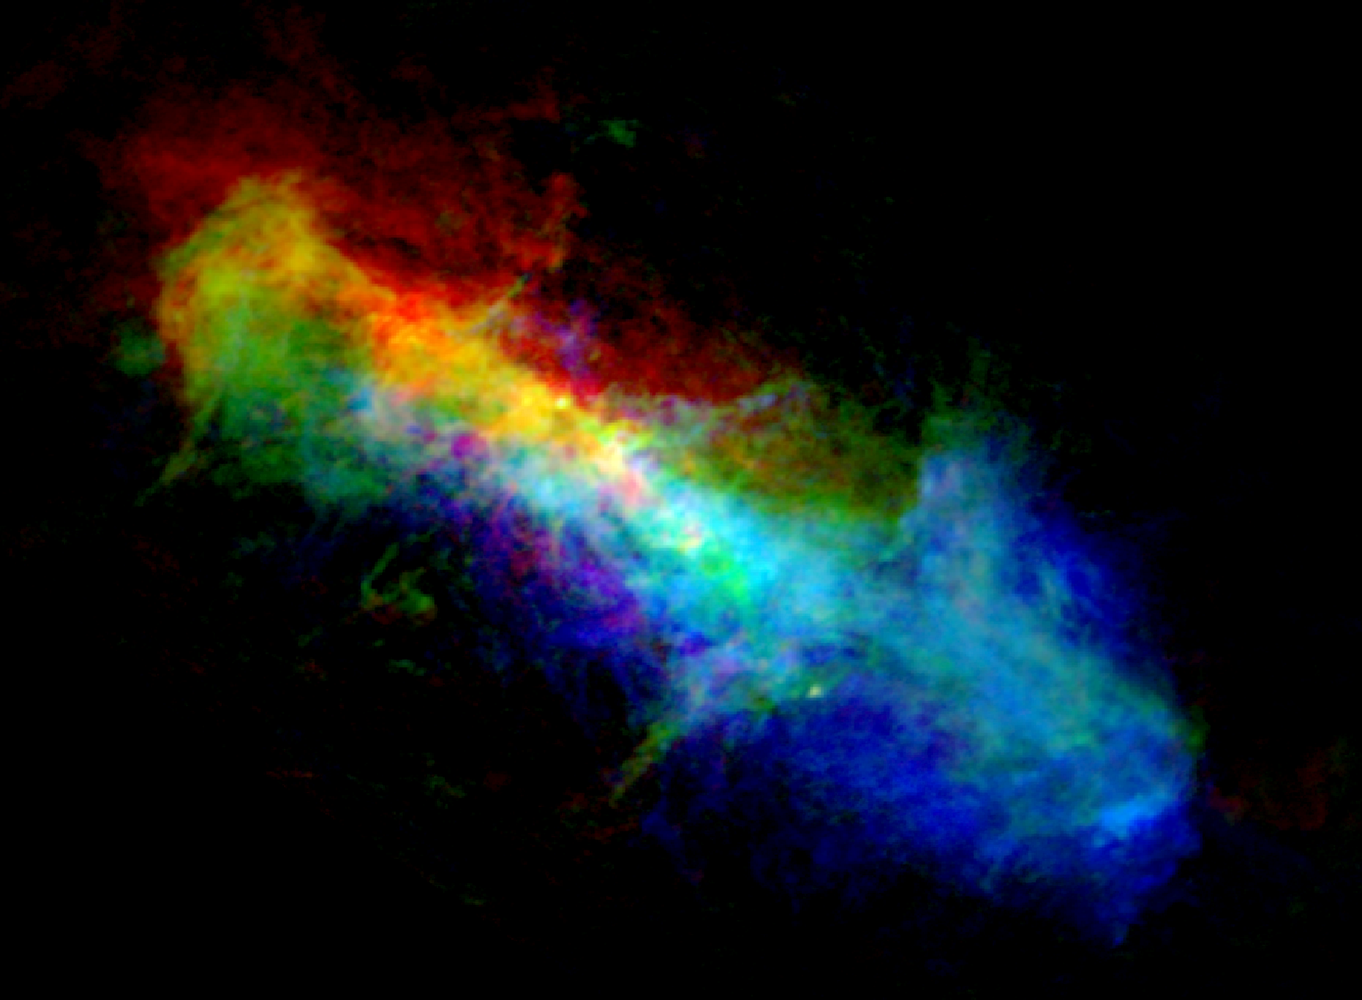
\includegraphics[width=0.95\paperwidth]{thesis/images/frontmatter/cover.png}
  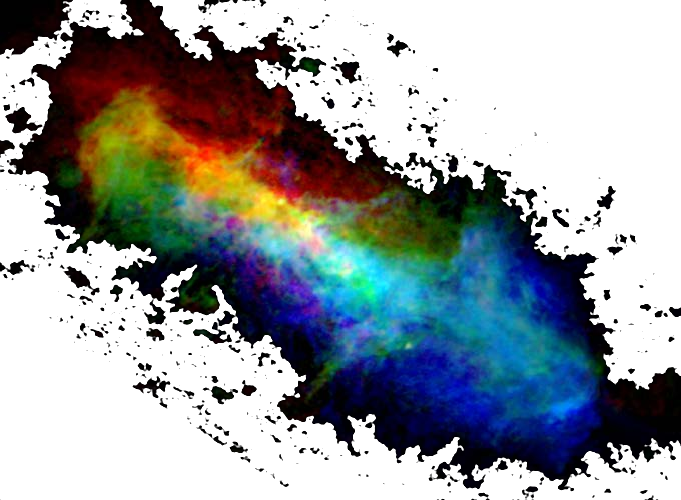
\includegraphics[width=0.95\paperwidth]{thesis/images/frontmatter/cover2.pdf}
  }%
}
\BgThispage

\begin{center}
    \color{white}
    \vspace{1cm}
    
    \resizebox{\linewidth}{!}{\textsc{\myTitle}}
    
    \vspace{1.5cm}
    \resizebox{\linewidth}{!}{\mySubtitle}

    \vfill
    \Large{A PhD Thesis in Astronomy put forward by \\ \myName}\\
    \vspace{0.5cm}
\end{center}


\clearpage
\restoregeometry

%*******************************************************
% Cover page backside
%*******************************************************
\thispagestyle{empty}
%\pdfbookmark[1]{Titel}{title}
%*******************************************************

% \newgeometry{centering}    %%% make the page centered on paper

% \begin{center}
%     {\large \color{CTtitle}
%         \spacedallcaps{\myTitle}
%     }
% \end{center}    

% \vfill

% \hspace{2cm}    
% \begin{tabular}{ll}
%     {\color{CTtitle} \spacedallcaps{Referees:}} & {\large \myExaminerOne}\\
%                                                 & {\large \myExaminerTwo}\\
% \end{tabular}


% \restoregeometry

\hfill
\vfill
\noindent

\textit{\textbf{Cover design:} 
The molecular gas in \ngc253 traced by carbon monoxide (CO). The three-color composite shows CO gas at the systemic velocity in green, gas approaching the observer in blue and receding gas in red. The rotating disk of molecular gas produces a color gradient (red -- green -- blue) from top left to bottom right. Seemingly mismatching structures all along the lower left and upper right edges of the disk highlight the abundant molecular streamers that are driven out of the galaxy by stellar feedback.
}

\vspace{1cm}
\textit{\textbf{Flipbook:}
This thesis is in large parts based on a dataset obtained with the ALMA interferometer. Such datasets contain three dimensional information (two spatial, one velocity dimensions) that are impossible to present in a printed document. Instead, images in the bottom left and right corner show the spatial information in succession of increasing velocity. When quickly scrolled through as a flipbook, the images show the rotating molecular gas disk in the center of \ngc253 similar to the movie function in common data visualization tools.
}
%*******************************************************
% Title page
%*******************************************************
\thispagestyle{empty}
%\pdfbookmark[1]{Titel}{title}
%*******************************************************

\newgeometry{centering}    %%% make the page centered on paper

\begin{center}
    {\small \color{CTtitle}
        \spacedallcaps{Dissertation}\\
        \spacedallcaps{submitted to the}\\
        \spacedallcaps{Combined Faculty of Natural Sciences and Mathematics}\\
        \spacedallcaps{of Heidelberg University, Germany}\\
        \spacedallcaps{for the degree of}\\
        \spacedallcaps{Doctor of Natural Sciences}
    }
    
    \vfill
    
    {\small \color{CTtitle} \spacedallcaps{Put forwards by}}\\ {\large \myName} \\ \medskip
    {\small \color{CTtitle} \spacedallcaps{born in:}} {\large \myBirthplace} \\
    {\small \color{CTtitle} \spacedallcaps{Oral examination:}} {\large \myOraldate} \\
    
\end{center}

\restoregeometry
\thispagestyle{empty}

\hfill
\vfill

\noindent \myName: \textit{\myTitle\ -- \mySubtitle} %\myDegree,
\\ 
\textcopyright\ \myTime

\bigskip

\noindent \hspace{-3mm}
\begin{tabular}{ll}
Supervisor:       & \mySupervisor \\
Advisers:         & \myAdviserOne, \myAdviserTwo \\
Oral examination: & \myOraldate \\
Examiners:        & \myAdviserOne, \myAdviserTwo\\
                  & \myExaminerOne, \myExaminerTwo\\
\end{tabular}


\cleardoublepage%*******************************************************
% Dedication
%*******************************************************
\thispagestyle{empty}
\phantomsection
\pdfbookmark[1]{Dedication}{Dedication}

\vspace*{3cm}

\begin{flushright}
    {\Large
    \textit{Nature's imagination is better than yours, and she is under no obligation to make herself comprehensible.}
    }
    \\ \bigskip
    {\large
    \href{https://www.youtube.com/watch?v=0R7EN_GTAlw}{\textbf{Exurb1a --- Letter to Marble 3}}
    }

    % Stop procrastinating. \\ \medskip
    % Now. \\ \bigskip
    % --- Exurb1a
\end{flushright}

% force next page to be empty as well
% otherwise it would have a tab bar already
\newpage
\thispagestyle{empty}


\BeginFlip
\cleardoublepage%*******************************************************
% Abstract
%*******************************************************

\chapter*{Abstract}
\chaptermark{abstract}

\renewcommand{\abstractname}{Abstract}
\pdfbookmark[1]{Abstract}{Abstract}
\addcontentsline{toc}{chapter}{\tocEntry{Abstract}}

\begingroup
\let\clearpage\relax
\let\cleardoublepage\relax
\let\cleardoublepage\relax


%%%%%%%%%%%%%%%%%%%%%%%%%%%%%%%%%%%%%%%%%%%%%%%%%%%%%%%%%%%%%%%%%%%%%%%%%%%%%%%%%%%%%%%%%%%%%%%%%%%%

Starburst galaxies are characterized by intense star formation at high star formation rate surface densities and short gas depletion times. 
Strong stellar feedback drives galaxy-scale winds and outflows in all gas phases, i.e. ionized, neutral and molecular.
The extreme conditions in local starburst galaxies are thought to be similar to those in typical high-redshift star forming galaxies, e.g. at the peak of the cosmic star formation history.

In this thesis, we present and analyze 0.15\arcsec ($\sim2.5$\,pc) resolution ALMA \co32 observations of the nuclear starburst in \ngc253. 
Using this data, we study the molecular outflow in unprecedented detail, zoom into \ngc253's super star clusters (SSCs) and compare the starburst to the similar but more quiescent center of the Milky Way.

Firstly, we kinematically decompose the molecular gas emission in \ngc253 into a disk and non--disk component to then separate out the molecular outflow. We systematically improve on previous measurement and obtain mass outflow rates $\dot{M} = 14-39$\,\Msunyr for the starburst. %($SFR \sim 2$\,\Msunyr).
The kinetic energy and momentum of the molecular outflow dominates over the other gas phases and is consistent with being supplied by the starburst at a few percent efficiency.

Secondly, we study the physical and chemical conditions in the molecular gas in the (proto-)SSCs in \ngc253, the places where future outflows will be launched from. The SSCs differ significantly in chemical complexity and show up to 55 lines belonging to 14 different chemical species. Spectral modelling allows us to infer spectral line ratios and physical properties.
The molecular gas in the SSCs is hot, consistent with UV photon-dominated chemistry and permeated by intense infrared radiation.

Thirdly, we compare the molecular cloud properties in the starbursting center of \ngc253 and the Milky Way Galactic Center (GC), that shares similar properties as \ngc253.
Using a structure identification algorithm on resolution-, area- and noise-matched datasets allows for a direct comparison of the kinematic structure.
Through common cloud scaling relations, we infer a high external pressure ($P_\mathrm{ext} \sim 10^{7-7.5}$\,K\,\pcm3) in \ngc253 and a significant amount of unbound (non-self-gravitating) molecular gas that is characterized by high velocity dispersion.

In summary, in this thesis we could follow the life cycle of a molecular outflow from an actively star forming molecular cloud before the launching of an outflow all the way out to distances that are hundreds of parsecs above the starburst disk where the outflow fades away.


%%%%%%%%%%%%%%%%%%%%%%%%%%%%%%%%%%%%%%%%%%%%%%%%%%%%%%%%%%%%%%%%%%%%%%%%%%%%%%%%%%%%%%%%%%%%%%%%%%%%

% \vfill
\newpage

\begin{otherlanguage}{ngerman}

\chapter*{Zusammenfassung}
\pdfbookmark[1]{Zusammenfassung}{Zusammenfassung}

%%%%%%%%%%%%%%%%%%%%%%%%%%%%%%%%%%%%%%%%%%%%%%%%%%%%%%%%%%%%%%%%%%%%%%%%%%%%%%%%%%%%%%%%%%%%%%%%%%%%

Starburst-Galaxien sind charakterisiert durch intensive Sternentstehung mit hohen Flächendichten der  Sternentstehungsrate und schnellem Verbrauch ihres Gases.
Starke stellare Rückkopplungsmechanismen erzeugen Winde und Ausflüsse auf galaktischen Skalen in allen Gasphasen, d. h. ionisiert, neutral and molekular.
Es wird davon ausgegangen, dass die extremen Bedingungen in lokalen Starburst-Galaxien ähnlich denen in typischen hochrotverschobenen Galaxien mit aktiver Sternentstehung sind. 

In dieser Arbeit präsentieren und analysieren wir ALMA Beobachtungen der nuklearen Starburst-Galaxie \ngc253 mit 0.15\arcsec ($\sim 2.5$\,pc) Auflösung.
Mithilfe dieser Daten studieren wir den molekularen Ausfluss in nie dagewesenem Detailreichtum, zoomen in die Supersterncluster (SSCs) und vergleichen den Starburst mit dem ähnlichen, aber ruhigeren Zentrum der Milchstraße.

Wir zerlegen die beobachtete Emission des molekularen Gases in \ngc253 in Scheiben- und Nicht-Scheiben-Komponenten, um daraufhin den molekularen Ausfluss zu identifizieren.
Wir verbessern systematisch vorherige Messungen und erhalten Ausflussmassenraten $\dot{M} = 14-39$\,\Msunyr für den Starburst.
Die kinetische Energie und der Impuls des molekularen Ausflusses dominieren über die anderen Gasphasen.
Energie und Impuls werden vom Starburst erzeugt und mit wenigen Prozent Effzienz an das molekulare Gas übertragen.

Desweiteren untersuchen wir die physikalischen und chemischen Bedingungen im molekularen Gas der (proto-)SSCs in \ngc253, der Orte an denen zukünftige Ausflüsse ausgeschleudert werden.
Die SSCs unterscheiden sich signifikant in ihrer chemischen Komplexität und zeigen bis zu 55 Spektrallinien von 14 verschiedenen Molekülen.
Durch Modellierung der Spektren erhalten wir Linienverhältnisse und physikalische Eigenschaften.
Das molekulare Gas in den SSCs ist heiß, konsistent mit Chemie dominiert von UV Photonen und durchdrungen von intensiver infraroter Strahlung.

Zuletzt vergleichen wir die Eigenschaften der molekularen Wolken im Starburst im Zentrum von \ngc253 mit dem Galaktischen Zentrum der Milchstraße, das ähliche Eigenschaften wie \ngc253 aufweist.
Mithilfe eines Algorithmus zur Strukturidentifikation, angewendet auf Daten angeglichener Auflösung, Abdeckung und Rauschens, wird die kinematische Struktur verglichen.
Skalierungsbeziehungen der Wolken zeigen hohen externen Druck ($P_\mathrm{ext} \sim 10^{7-7.5}$\,K\,\pcm3) auf die Wolken und signifikante Mengen an ungebundenem (nicht selbst-gravitierendem) molekularem Gas, das durch hohe Geschwindigkeitsdispersion charakterisiert wird.

Zusammenfassend folgt diese Arbeit dem Leben eines molekularen Ausflusses von einer aktiv sternbildenden molekularen Wolke vor Auswurf eines Ausflusses bis hin zu hunderten Parsec über dem Starburst, wo der Ausfluss verblasst.


%%%%%%%%%%%%%%%%%%%%%%%%%%%%%%%%%%%%%%%%%%%%%%%%%%%%%%%%%%%%%%%%%%%%%%%%%%%%%%%%%%%%%%%%%%%%%%%%%%%%

\end{otherlanguage}

\endgroup

\vfill

\cleardoublepage%*******************************************************
% Publications
%*******************************************************
\pdfbookmark[1]{Publications}{publications}
\chapter*{Publications}
\chaptermark{publications}
\addcontentsline{toc}{chapter}{\tocEntry{Publications}}


During my PhD studies I was leading or contributing author of the following publications. The work presented in Chapters~\ref{chapter: outflow}, \ref{chapter: SSCs} and \ref{chapter: dendro} has been presented in Krieger et al. (2019), Krieger et al. (2020a) and Krieger et al. (2020b), respectively.


\vspace{\baselineskip}\textbf{\textsc{Leading author:}}
\vspace{0.5\baselineskip}

\publication{
    \textbf{N. Krieger}, A. D. Bolatto, A. K. Leroy, R. C. Levy, E. A.C. Mills, D. S. Meier, S. Veilleux, F. Walter, A. Weiß
    }{
    The Molecular ISM in the Super Star Clusters of the Starburst NGC253.
    }{
    2020a, submitted to The Astrophysical Journal
    }

\publication{
    \textbf{N. Krieger}, A. D. Bolatto, E. W. Koch, A. K. Leroy, E. Rosolowsky, F. Walter, A. Weiß, D. J. Eden, R. C. Levy, D. S. Meier, E. A. C. Mills, Toby Moore, Jürgen Ott, Yang Su, S. Veilleux
    }{
    The turbulent gas structure in the centers of NGC253 and the Milky Way.
    }{
    2020b, submitted to The Astrophysical Journal
    }

\publication{
    \textbf{N. Krieger}, A. D. Bolatto, F. Walter, A. K. Leroy, L. K. Zschaechner, D. S Meier, J. Ott, A. Weiss, E. A. C. Mills, R. C. Levy, S. Veilleux, M. Gorski.
    }{
    The Molecular Outflow in \ngc253 at a Resolution of Two Parsecs.
    }{
    The Astrophysical Journal, 2019 vol. 881 (1) p. 43.
    }

\publication{
    \textbf{N. Krieger}, J. Ott, H. Beuther, F. Walter, J. M. D. Kruijssen, D. S. Meier, E. A. C. Mills, Y. Contreras, P. Edwards, A. Ginsburg, C. Henkel, J. D. Henshaw, J. M. Jackson, J. Kauffmann, S. N. Longmore, S. Martín, M. R. Morris, T. Pillai, M. Rickert, E. Rosolowsky, H. Shinnaga, A. Walsh, F. Yusef-Zadeh, Q. Zhang.
    }{
    The Survey of Water and Ammonia in the Galactic Center (SWAG): Molecular Cloud Evolution in the Central Molecular Zone.
    }{
    The Astrophysical Journal, 2017 vol. 850 (1) p. 77.
    }


\vspace{\baselineskip}\textbf{\textsc{Contributing author:}}
\vspace{0.5\baselineskip}

\publication{
    K. L. Emig, A. D. Bolatto, A. K. Leroy, E. A. C. Mills, M. J. Jimenez Donaire, A. G. G. M. Tielens, L. Levy, \textbf{N. Krieger}, E. Ostriker, E. Rosolowsky,  S. Veilleux
    }{
    Star Clusters in the Central Starburst of \ngc4945
    }{
    Submitted to the The Astrophysical Journal
    }

\publication{
    J. M. D. Kruijssen, J. E. Dale, S. N. Longmore, D. L. Walker, J. D. Henshaw, S. M. R. Jeffreson, M. A. Petkova, A. Ginsburg, A. T. Barnes, C. D. Battersby, K. Immer, J. M. Jackson, E. R. Keto, \textbf{N. Krieger}, E. A C Mills, A. Sánchez-Monge, A. Schmiedeke, S. T. Suri, Q. Zhang.
    }{
    The dynamical evolution of molecular clouds near the Galactic Centre - II. Spatial structure and kinematics of simulated clouds.
    }{
    Monthly Notices of the Royal Astronomical Society, 2019 vol. 484 (4) pp. 5734-5754.
    }
    
\publication{    
    A. K. Leroy, A. D. Bolatto, E. C. Ostriker, F. Walter, M. Gorski, A. Ginsburg, \textbf{N. Krieger}, R. C. Levy, D. S. Meier, E. A. C. Mills, J. Ott, E. Rosolowsky, T. A. Thompson, S. Veilleux L. K. Zschaechner.
    }{
    Forming Super Star Clusters in the Central Starburst of NGC 253.
    }{
    The Astrophysical Journal, 2018 vol. 869 (2) p. 126.
    }
    
\publication{    
    L. K. Zschaechner, A. D. Bolatto, F. Walter, A. K. Leroy, C. Herrera, \textbf{N. Krieger}, J. M. D. Kruijssen, D. S Meier, E. A C Mills, J. Ott, S. Veilleux, A. Weiß.
    }{
    Spatially Resolved 12CO(2–1)/12CO(1–0) in the Starburst Galaxy NGC 253: Assessing Optical Depth to Constrain the Molecular Mass Outflow Rate.
    }{
    The Astrophysical Journal, 2018 vol. 867 (2) p. 111.
    }


\vspace{\baselineskip}\textbf{\textsc{Conference Proceedings:}}
\vspace{0.5\baselineskip}

\publication{    
    J. Ott, D. S Meier, A. Ginsburg, F. Yusef-Zadeh, \textbf{N. Krieger}, C. Jäschke.
    }{
    SWAG: Distribution and Kinematics of an Obscured AGB Population toward the Galactic Center.
    }{
    Proceedings IAU Symposium No. 343: Why Galaxies Care About AGB Stars: A Continuing Challenge through Cosmic Time, 2019, pp. 485-486.
    }

\publication{
    J. Ott, D. S Meier, \textbf{N. Krieger}, A. Ginsburg, T. Candelaria.
    }{
    Survey of Water and Ammonia in the Galactic center (SWAG): Morphologies of Molecular Tracers.
    }{
    Proceedings American Astronomical Society Meeting No. 233, 2019, p. 267.01.
    }
    
\publication{    
    J. Ott, \textbf{N. Krieger}, M. Rickert, D. S Meier, A. Ginsburg, F. Yusef-Zadeh.
    }{SWAG Water Masers in the Galactic Center.
    }{
    Proceedings IAU Symposium No. 336: Astrophysical Masers: Unlocking the Mysteries of the Universe, 2017
    }
    
\publication{    
    M. Rickert, F. Yusef-Zadeh, J. Ott, D. S Meier, \textbf{N. Krieger}.
    }{
    High Resolution Surveys of the Water and Methanol Star Formation Masers in the Central Molecular Zone.
    }{
    Proceedings American Astronomical Society Meeting No. 229, 2017, p. 216.06.
    }
    
\publication{    
    \textbf{N. Krieger}, J. Ott, F. Walter, J. M. D. Kruijssen, H. Beuther.
    }{
    Temperature Evolution of Molecular Clouds in the Central Molecular Zone.
    }{
    Proceedings IAU Symposium No. 322: The Multi-Messenger Astrophysics of the Galactic Centre, 2016, pp. 1-2.
    }
    
\publication{    
    J. Ott, D. S Meier, \textbf{N. Krieger}, M. Rickert.
    }{
    SWAG: Survey of Water and Ammonia in the Galactic Center.
    }{
    Proceedings IAU Symposium No. 322: The Multi-Messenger Astrophysics of the Galactic Centre, 2016, pp. 1-2.
    }

\cleardoublepage%*******************************************************
% Acknowledgments
%*******************************************************
\pdfbookmark[1]{Acknowledgments}{acknowledgments}
\chaptermark{acknowledgements}

% \begin{flushright}{\slshape
%     We have seen that computer programming is an art, \\
%     because it applies accumulated knowledge to the world, \\
%     because it requires skill and ingenuity, and especially \\
%     because it produces objects of beauty.} \\ \medskip
%     --- \defcitealias{knuth:1974}{Donald E. Knuth}\citetalias{knuth:1974} \citep{knuth:1974}
% \end{flushright}



\bigskip

\begingroup
\let\clearpage\relax
\let\cleardoublepage\relax
\let\cleardoublepage\relax

\chapter*{Acknowledgments}
\addcontentsline{toc}{chapter}{\tocEntry{Acknowledgments}}

First of all, I would like to express my gratitude to my supervisor Dr. Fabian Walter. He is the most helpful and nice supervisor I could have imagined. I could not know what would happen when I stepped into his office seven and a half years ago on the look for potential Bachelor thesis projects. The academic work and personal relationship between supervisor and student turned out so inspiring that I could have done only worse when searching for another supervisor for my Master's and PhD theses. Over the years, I have always left his office with new hope in times of trouble, the feeling that it all will work and anything is possible.

At this stage, I would also like to thank my friend Dr. Miguel Querejeta for showing me around at MPIA. If not for him, I might have never ended up on the mountain and certainly not in the group of Fabian.

Thank you to all my friends and colleagues at MPIA for the helpful discussions, mutual support and all the fun.

Astrophysical research is a joint effort of many people. Thank you to my colleagues and collaborators in various projects over the years.
A special thanks I want to address to Dr. J\"urgen Ott at NRAO who was my first academic contact outside MPIA seven years ago, whom I visited numerous time and a close collaborator ever since. Thank you for the great times in Socorro and, not to forget, for letting me borrow your car.

I would like to thank the members of my thesis committee who are also the referees of my thesis, Prof. Dr. Hans-Walter Rix and Prof. Dr. Ralf Klessen, for their time and support.
Thank you to Prof. Dr. Eva Grebel and Prof. Dr. Bj\"orn-Malte Sch\"afer for kindly agreeing to be members of the thesis defense committee.

\vspace{\baselineskip}

Life is much more than just work, as interesting as it might be. Athletics has always played a major role in my life and contributed so many things to me and my life.
Thank you to all my friends at USC Heidelberg and TSG 78 Heidelberg who helped me to maintain a healthy balance between work, sports and other activities. Training sessions, competitions, training camp and all the other fun activities we did together helped me through the harder times of my thesis.

\vspace{\baselineskip}

I am deeply grateful for the support from my parents over the years. A vital element for this thesis to ever exist was their encouragement to follow my passion and study physics in Heidelberg. Thank you for your support in all aspects of my life.

\vspace{\baselineskip}

Thank you Sophia for your unconditional love, for the practical and emotional support, especially, during the stressful times towards the end of my thesis.


\endgroup


\newpage
\chaptermark{}
\cleardoublepage%*******************************************************
% Table of Contents
%*******************************************************
\pagestyle{scrheadings}
%\phantomsection
\pdfbookmark[1]{\contentsname}{tableofcontents}

\setcounter{tocdepth}{1}    % <-- 1: sections, 2: subsections
\setcounter{secnumdepth}{3} % <-- 3 numbers up to subsubsections
\manualmark
\markboth{\spacedlowsmallcaps{\contentsname}}{\spacedlowsmallcaps{\contentsname}}

\renewcommand{\cftpartleader}{\cftdotfill{\cftdotsep}} % dots for parts
\renewcommand{\cftchapleader}{\cftdotfill{\cftdotsep}} % dots for chapters
\renewcommand{\cftsecleader}{\cftdotfill{\cftdotsep}}  % dots for sections

\pdfbookmark[1]{Contents}{Contents}
\markboth{\spacedlowsmallcaps{Contents}}{\spacedlowsmallcaps{Contents}}
\chapter*{Contents}
\addcontentsline{toc}{chapter}{\tocEntry{Contents}}

\renewcommand\contentsname{} % the empty name
\begingroup
\let\clearpage\relax
\vspace{-3cm} % the removed space. Set as appropriate
\tableofcontents
\endgroup

% \tableofcontents

\automark[section]{chapter}
\renewcommand{\chaptermark}[1]{\markboth{\spacedlowsmallcaps{#1}}{\spacedlowsmallcaps{#1}}}
\renewcommand{\sectionmark}[1]{\markright{\textsc{\thesection}\enspace\spacedlowsmallcaps{#1}}}


%*******************************************************
% List of Figures and of the Tables
%*******************************************************

\clearpage
% \pagestyle{empty} % Uncomment this line if your lists should not have any headlines with section name and page number

%*******************************************************
% List of Figures
%*******************************************************

\begingroup
    \let\clearpage\relax
    \let\cleardoublepage\relax
    %\phantomsection
    %\addcontentsline{toc}{chapter}{\listfigurename}
    \pdfbookmark[1]{\listfigurename}{lof}
    \pdfbookmark[1]{List of Figures}{List of Figures}
    \markboth{\spacedlowsmallcaps{List of Figures}}{\spacedlowsmallcaps{List of Figures}}
    \chapter*{List of Figures}
    \chaptermark{list of figures}
    \renewcommand{\listfigurename}{}
    \begingroup
    \let\clearpage\relax
    \vspace{-3cm} % the removed space. Set as appropriate
    \listoffigures
    \endgroup
\endgroup

\clearpage

%*******************************************************
% List of Tables
%*******************************************************

\begingroup
    \let\clearpage\relax
    \let\cleardoublepage\relax
    %\phantomsection
    %\addcontentsline{toc}{chapter}{\listtablename}
    \pdfbookmark[1]{\listtablename}{lot}
    \pdfbookmark[1]{List of Tables}{List of Tables}
    \markboth{\spacedlowsmallcaps{List of Tables}}{\spacedlowsmallcaps{List of Tables}}
    \chapter*{List of Tables}
    \chaptermark{list of tables}
    \renewcommand{\listtablename}{}
    \begingroup
    \let\clearpage\relax
    \vspace{-3cm} % the removed space. Set as appropriate
    \listoftables
    \endgroup
\endgroup

\clearpage

%*******************************************************
% List of Listings
%*******************************************************

% \chaptermark{list of listings}
% \begingroup
%     \let\clearpage\relax
%     \let\cleardoublepage\relax
    % %\phantomsection
    % %\addcontentsline{toc}{chapter}{\lstlistlistingname}
    % \pdfbookmark[1]{\lstlistlistingname}{lol}
    % \lstlistoflistings
% \endgroup

% \vspace{8ex}

%*******************************************************
% Acronyms
%*******************************************************

% \chaptermark{acronyms}
% \begingroup
%     \let\clearpage\relax
%     \let\cleardoublepage\relax
%     %\phantomsection
%     \pdfbookmark[1]{Acronyms}{acronyms}
%     \markboth{\spacedlowsmallcaps{Acronyms}}{\spacedlowsmallcaps{Acronyms}}
%     \chapter*{Acronyms}
%     \begin{acronym}[UMLX]
%         \acro{DRY}{Don't Repeat Yourself}
%         \acro{API}{Application Programming Interface}
%         \acro{UML}{Unified Modeling Language}
%     \end{acronym}
% \endgroup



%********************************************************************
% Mainmatter
%*******************************************************

\cleardoublepage
\pagestyle{scrheadings}
\pagenumbering{arabic}
%\setcounter{page}{90}

% use \cleardoublepage here to avoid problems with pdfbookmark
% \cleardoublepage

\cleardoublepage%%%%%%%%%%%%%%%%%%%%%%%%%%%%%%%%%%%%%%%%%%%%%%%%%%%%%%%%%%%%%%%%%%%%%%%%%%%%%%%%%%%%%%%%%%%%%%%%%%%%

\part*{Introduction}
\label{part: introduction}

%%%%%%%%%%%%%%%%%%%%%%%%%%%%%%%%%%%%%%%%%%%%%%%%%%%%%%%%%%%%%%%%%%%%%%%%%%%%%%%%%%%%%%%%%%%%%%%%%%%%


%%%%%%%%%%%%%%%%%%%%%%%%%%%%%%%%%%%%%%%%%%%%%%%%%%%%%%%%%%%%%%%%%%%%%%%%%%%%%%%%%%%%%%%%%%%%%%%%%%%%

\chapter{Motivation}
\chaptermark{motivation}
\label{part: motivation}

%%%%%%%%%%%%%%%%%%%%%%%%%%%%%%%%%%%%%%%%%%%%%%%%%%%%%%%%%%%%%%%%%%%%%%%%%%%%%%%%%%%%%%%%%%%%%%%%%%%%

% Motivation is what's needed to get out of bed in the morning.\\
% \hspace*{\fill} --- me.
% \vspace{1cm}

Understanding our place in the universe and how the universe came to be is one of the most basic existential desires of humankind -- probably since humans evolved far enough to develop such complex thoughts. The history of the universe is complicated and long, almost 14 billion years by now. We have learned much through astronomy and astrophysical research came closer to answers to these basic questions. However, many fundamental questions are still open. For instance, how and why did we end up on the blue planet thinking about all of this?
\vspace{0.25\baselineskip}

Exploring where we come from and how we came to be touches on the fields of cosmology, astrophysics, geology, biology and more. After the big bang and the early phases of the universe, galaxies of dark matter, gas and stars started to assemble. Through merging and accretion of primordial gas, these galaxies built up their stellar content with a whole system of planets for each star. The cosmic star formation rate accelerated quickly in the early universe, slowed down and eventually started to decline after two to three billion years. This means many if not most stars in our own Milky Way and other local galaxies formed billions of years ago when the conditions were different from today.

Even for down-to-earth questions such as how intelligent life could develop on earth, it is therefore necessary to understand star formation in general and in particular how star formation worked at the time the sun and our planetary system formed about five billion years ago. Traces of how the sun formed are long gone but thanks to the finite speed of light, we are able to observe past times when we observe objects far away from us.
Studying star forming galaxies that are billions of lightyears away from us in the required detail is not possible with today's technology but luckily there are local galaxies that are very similar in their properties. The mentioned decline of the star formation rate history means that what used to be a normal star forming galaxy like all the others billions of years ago, today, is an exceptionally intensely star forming -- star bursting -- galaxy.

Many details of starbursts are not yet understood. Star formation is a complex process covering spatial scales from galaxy sizes down to single stars over many orders of magnitude. The gas and dust in the interstellar medium from which stars form is already a thermodynamically complex mixture of gases, solids and plasmas. The picture gets even more complex when considering the interaction between (forming) stars and the interstellar medium. This feedback can have diametral effects in shutting down star formation or enhancing it depending on the details of the exact situation. Gaseous outflows driven by feedback from stars or actively accreting black holes are an integral part in determining the evolution of a galaxy.

In this thesis, I work on certain aspects of star formation, stellar feedback and galactic outflows to deepen humankind's understanding of star formation and the evolution of the universe.
I characterize outflows of molecular gas, zoom into the environment of forming super star clusters and examine the feedback effects on dense molecular gas in galactic centers.
Each of these works is only a tiny piece in the grand puzzle that is the universe, but finding each piece and putting it in the right location is necessary to build up the full picture of the universe and the life within it.


\newpage
\begin{overpic}[width=\textwidth]{images/chapters/introduction/ism/overview.pdf}
    \label{introduction: figure: topics overview}
    \put (5,90) {\color{white} \scalebox{2}{What this thesis addresses:}}
    \put (5,82) {\color{white} \Large \textbf{interstellar medium}}
        \put (5,78) {\color{white} \large Chapters \ref{introduction: chapter: ism}, \ref{chapter: outflow}, \ref{chapter: outflow catalog}, \ref{chapter: SSCs}, \ref{chapter: dendro}}
    \put (38,76) {\color{white} \Large \textbf{star formation}}
        \put (38,72) {\color{white} \large Chapters \ref{introduction: chapter: star formation}, \ref{chapter: outflow}, \ref{chapter: outflow catalog}, \ref{chapter: SSCs}, \ref{chapter: dendro}}
    \put (8,65) {\color{white} \Large molecular gas}
        \put (8, 61){\color{white}\large Chapters \ref{introduction: chapter: ism}, \ref{introduction: chapter: star formation}, \ref{chapter: outflow}, \ref{chapter: outflow catalog}, \ref{chapter: SSCs}, \ref{chapter: dendro}}
    \put (7,23) {\color{white} \Large star formation fueling}
        \put (7,19) {\color{white} \large Chapters \ref{introduction: chapter: star formation}, \ref{chapter: SSCs}}
    \put (36,33) {\color{white} \Large embedded (proto-)}
    \put (36,30) {\color{white} \Large super star cluster}
        \put (36,26) {\color{white} \large Chapters \ref{introduction: section: star formation: SSCs}, \ref{chapter: SSCs}}
    \put (70,49) {\color{white} \Large stellar feedback}
        \put (70,45) {\color{white} \large Chapters \ref{introduction: chapter: star formation}, \ref{chapter: outflow}, \ref{chapter: outflow catalog}, \ref{chapter: SSCs}, \ref{chapter: dendro}}
    \put (52,20) {\color{white} \Large outflow driving}
        \put (52,16) {\color{white} \large Chapters \ref{chapter: outflow}, \ref{chapter: outflow catalog}}
    \put (72,73) {\color{white} \Large cloud destruction}
        \put (81.5,69) {\color{white} \large Chapters \ref{introduction: chapter: star formation}, \ref{chapter: SSCs}}
    \put (5,7) {\color{white} \Large The life cycle of a molecular outflow from prior to}
    \put (5,3) {\color{white} \Large launching by stellar feedback to fading far above the galactic disk.}
\end{overpic}

\vspace{0.5cm}
\begin{tabular}{@{}ll}
    \textit{Images:} & Super star cluster Westerlund~1, HST/NASA/ESA, HST ID: \href{https://www.spacetelescope.org/images/potw1710a/}{potw1710a}\\
     & Milky Way panorama, ESO/S. Brunier, ESO ID: \href{https://www.eso.org/public/images/eso0932a/}{eso0932a}\\
    \textit{Composition:} & N. Krieger
\end{tabular}

%%%%%%%%%%%%%%%%%%%%%%%%%%%%%%%%%%%%%%%%%%%%%%%%%%%%%%%%%%%%%%%%%%%%%%%%%%%%%%%%%%%%%%%%%%%%%%%%%%%%

\chapter{The interstellar medium}
\chaptermark{the instellar medium}
\label{introduction: chapter: ism}

%%%%%%%%%%%%%%%%%%%%%%%%%%%%%%%%%%%%%%%%%%%%%%%%%%%%%%%%%%%%%%%%%%%%%%%%%%%%%%%%%%%%%%%%%%%%%%%%%%%%

Galaxies are complex objects build from dark matter and various phases of baryonic matter \citep[e.g.][]{1933AcHPh...6..110Z}. The different constituents are in constant interplay through gravitational, electro-magnetic and mechanical forces. 
The interstellar medium (ISM) is a cardinal point is these interactions \citep[e.g.][]{2016SAAS...43...85K} as the ISM contains large amounts of mass, stars form from it and return gas and energy to the ISM. 
A lack of suitable ISM can starve star formation and galaxy evolution but also boost it to extreme conditions.
In such violent environments, the ISM can even be expelled from its host galaxy and into the intergalactic medium \citep[e.g.][]{1971ApJ...165..381J}.

The term interstellar medium encompasses all baryonic matter between stars. This includes gas of various types and dust but also radiation is often considered a part of the ISM.
The ISM in early type (ellipticals) and irregular galaxies can be very different from the ISM in late type (spiral) galaxies. For now, we focus on the ISM in typical spiral, star-forming galaxies.


%%%%%%%%%%%%%%%%%%%%%%%%%%%%%%%%%%%%%%%%%%%%%%%%%%%%%%%%%%%%%%%%%%%%%%%%%%%%%%%%%%%%%%%%%%%%%%%%%%%%

\section{Phases of the ISM}
\label{introdution: section: ism: phases}

The ISM consists of several phases that are commonly grouped according to temperature and composition \citep[e.g.][]{2011piim.book.....D}.
\vspace{0.5\baselineskip}

\emph{Hot ionized medium} --- By volume, most ($\sim 50$\%) of the gas trapped by the gravity of a galaxy and its dark matter halo is hot ($T \GTRSIM 10^{5.5}$\,K). Heated by shocks and ionized by collisions, this phase is very thin ($n \LESS 0.01$ atoms per cubic cm).
\vspace{0.5\baselineskip}

\emph{Warm ionized medium} --- At lower temperatures of $T \sim 10^4$\,K, this phase typically fills $\sim10$\% of a galaxy's volume. Energetic photons from the galaxy provide the heating and ionize the gas. Its density is typically of order 1\,\pcm3.
\vspace{0.5\baselineskip}

\emph{Warm neutral medium} --- This phase is cool enough ($\sim 5000$\,K) to remain neutral. At $\sim 40$\% volume filling fraction, it overlaps spatially with warm and hot ionized medium. Its density of $\sim 1$\,\pcm3 and the large filling fraction shows that there can be substantial amounts of gas in this phase.
%The 21\,cm line of neutral hydrogen (\hi) is the main tracer of the warm neutral medium.
\vspace{0.5\baselineskip}

\emph{Cold neutral medium} --- Although virtually identical in composition to the warm neutral medium, the cold neutral medium is much colder ($T \sim 100$\,K) and denser (order of 30\,\pcm3). This is only possible due to shielding from radiation by outer gas layers in relatively compact aggregations. These clouds, therefore, occupy a small volume in a galaxy ($\sim 1$\%) primarily in a thin and thick disk, typically co-planar to the stellar disk.
\vspace{0.5\baselineskip}

\emph{Cold molecular medium} --- Only a tiny volume fraction of $\sim 0.1$\% of a spiral galaxy is filled by molecular gas. Shielding by layers of neutral gas are required to intercept radiation (electro-magnetic and cosmic rays) that can easily destroy molecular bonds. Within (giant) molecular clouds, the gas can efficiently cool down to $T \LESSSIM 100$\,K and may even reach $T \LESSSIM 10$\,K. The densities in molecular clouds range from hundreds to $\GTR 10^8$\,\pcm3 which can be enough to start gravitational collapse under its own weight in the star formation process (Chapter~\ref{introduction: chapter: star formation}).
\vspace{0.5\baselineskip}

The ISM phases are not stationary but in constant interaction and evolution. Heating and cooling can transfer mass, momentum and energy between the phases. Molecular gas can be dissociated and ionized by intense radiation and its constituent atoms feed the warm and hot ISM phases. Vice versa, ionized gas can recombine with electrons, radiatively cool and form molecules or even dust to replenish the cold ISM phases.

Typically, the ISM phases are roughly in pressure equilibrium. The thermal pressure is usually weak while magnetic and turbulent pressure dominate.
Gas not in equilibrium can be found as e.g. self-gravitating molecular gas (Section~\ref{introduction: section: star formation: sketch}) or outflows (Section~\ref{introduction: section: star formation: outflows}).


%%%%%%%%%%%%%%%%%%%%%%%%%%%%%%%%%%%%%%%%%%%%%%%%%%%%%%%%%%%%%%%%%%%%%%%%%%%%%%%%%%%%%%%%%%%%%%%%%%%%

\section{Elements in the ISM}
\label{introdution: section: ism: elements}

From Big Bang nucleosynthesis, hydrogen is the most common element in the universe with $\sim 90$\% abundance, followed by helium with $\sim 10$\% \citep[e.g.][]{1994ARA&A..32..191W}. Hence, the ISM phases are also dominated by hydrogen in the forms of ionized (\hii), neutral (\hi) and molecular (\htwo) hydrogen.
However, the heavy elements that were almost exclusively cooked up by stars \citep[e.g.][]{1988ccna.book.....R,2014PASA...31...30K}, are an important addition to the ISM. Their wide repertoire of electronic transitions allow for much more efficient cooling than pure hydrogen and helium, and thus regulate the heating/cooling of the ISM.
The most common elements in the ISM aside from hydrogen and helium are low atomic number elements, alpha elements with multiples of four atomic numbers (C, N, O, Ne, Mg, Si, S, Ar, Ca, Ti) and elements of the iron peak (Ti, V, Cr, Mn, Fe, Co, Ni) \citep[e.g.][]{1994ARA&A..32..191W}. 
Alpha elements are efficiently produced by alpha (helium core) capture in core-collapse (type II) supernovae while iron peak elements are synthesized alongside alpha elements in type Ia supernovae.
Hence, different forms of these elements provide crucial tracers to study the ISM. For instance, the spectral lines of ionized and neutral heavy elements reveal the hot and warm phases of the ISM. In the molecular phase, complex compounds with dozens of atoms can form and offer an overwhelming amount of spectral lines to study chemistry and physical conditions \citep[e.g.][]{1973ApJ...185..505H}. In dust grains, thousands to millions of atoms and molecules agglomerate and provide a surface for chemical reactions that cannot take place in the gas phase \citep[e.g.][]{2017MolAs...9....1W,2005JPhCS...6...18H}.


%%%%%%%%%%%%%%%%%%%%%%%%%%%%%%%%%%%%%%%%%%%%%%%%%%%%%%%%%%%%%%%%%%%%%%%%%%%%%%%%%%%%%%%%%%%%%%%%%%%%

\section{Molecular clouds}
\label{introdution: section: ism: molecular clouds}

Molecular gas typically resides in so-called molecular clouds of diffuse, filamentary and/or concentrated structures of various sizes. Most of the gas mass is found in giant molecular clouds (GMC) of $\sim5-200$\,pc with masses of typically $10^2 - 10^7$\,M$_{\odot}$ \citep[e.g.][]{2010ARA&A..48..547F}. More concentrated, smaller clouds are nested as substructure inside GMCs down to cloud cores on $\LESS 0.1$\,pc scales \citep[e.g.][]{1993prpl.conf..125B}. The number densities in clouds range from several cm$^{-3}$ up to $\GTR 10^8$\,cm$^{-3}$ in cloud cores. Despite their name, a significant amount of mass remains in an atomic state and typical molecular abundance ratios are M$_{H_2}$/M$_{HI} \sim0.3$ with 0.4\,dex scatter \citep[e.g.][]{1973AmSci..61..524S,2007prpl.conf...81B,2012MNRAS.424.2599C}. Significant quantities of dust can form and survive under molecular cloud conditions by (self-)shielding. The absorption of incident radiation can be observed as extinction in the visible to infrared spectrum \citep[e.g.][]{1921AN....213..351H,1976AJ.....81..308S,2007ARA&A..45..339B}.
%Cloud surface densities range from tens to $\GTR 200$\,M$_\odot$/pc$^2$ leading to visual extinction by gas and dust of $0.5\LESS \mathrm{A_V}\LESS 5$. 
Cloud population masses typically follow a power law mass spectrum dN/dM $\sim$ M$^{-\gamma}$ with $\gamma \LESS 2$ \citep[e.g.][and references therein]{2014PhR...539...49K} with few large, massive clouds and increasing numbers of small, low-mass clouds.

\begin{figure}
    \centering
    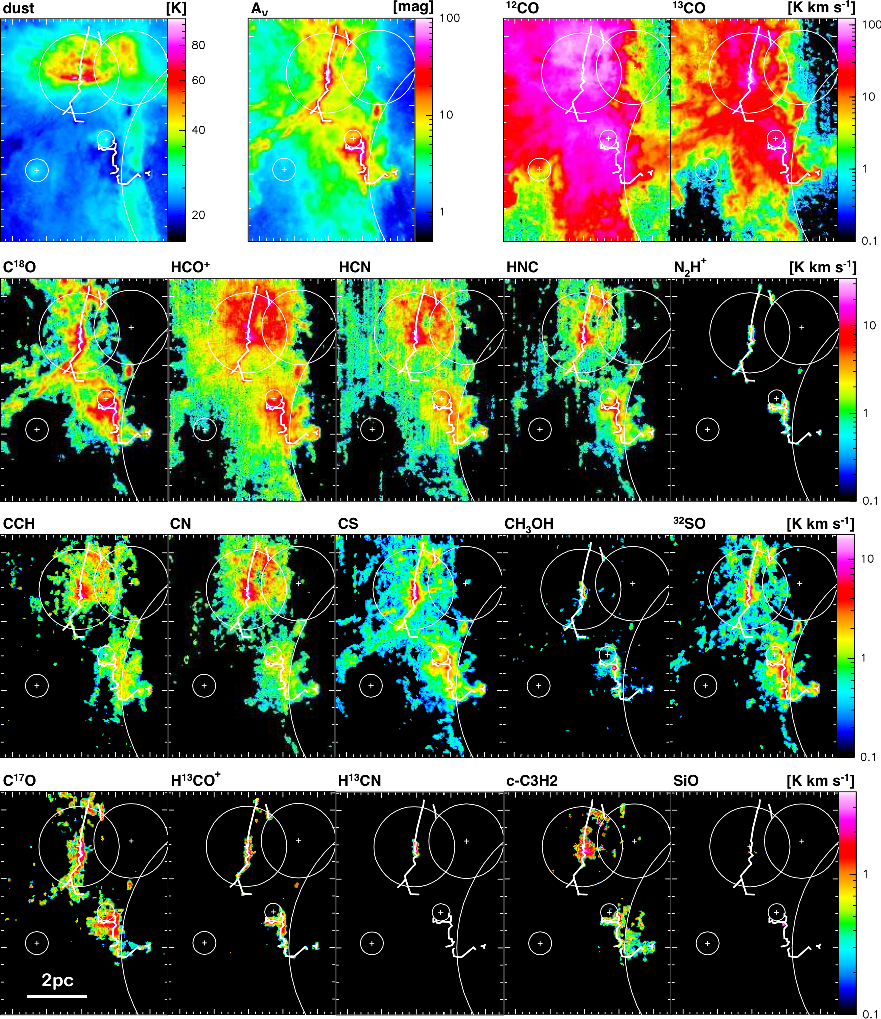
\includegraphics[width=\textwidth]{images/chapters/introduction/ism/Pety+16_overview.pdf}
    \caption[Distribution of molecules in Orion]{The distribution of molecules varies strongly within molecular clouds as shown here for Orion B \citep[adapted from figure 2]{2017A&A...599A..98P}. Less dense gas traced by CO is widespread around the central ridges seen in optical extinction (A$_\mathrm{v}$). The CO isotopologs $^{13}$CO, C$^{18}$O and C$^{17}$O are less and less abundant and trace increasingly dense regions within the cloud. The classical high density tracers HCN and HCO$^+$ are brightly detected over larger area of the cloud but other tracers better show the (projected) structures of the cloud internals. The shock tracer SiO is confined to one core and does not show in the rest of the cloud.}
    \label{introduction: figure: molecular cloud molecule distribution}
\end{figure}

The molecular content of a cloud is mainly H$_2$ by mass that survives dissociation by the shielding effect of outer layers of gas and dust. Towards the central regions, densities and path lengths to the outside increase, which is why more complex, less strongly bound and less abundant molecules are found there as shown in Figure~\ref{introduction: figure: molecular cloud molecule distribution} for a few tracers in the giant molecular cloud \ngc6334 \citep{2017A&A...599A..98P}. The temperature accordingly decreases towards the center because radiative cooling is possible by escaping photons of infrared or sub-mm lines while external heating sources are shielded by upper cloud layers. When internal heating mechanism start (e.g. star formation, Chapter~\ref{introduction: chapter: star formation}), the temperature structure becomes more complex.

The basic cloud properties size, linewidth and column density were empirically found to be related by \citet{Larson:1981jm} in three so-called Larson laws. These scaling relations can be explained theoretically with the gravitational and hydrodynamic properties and were re-examined frequently over the past 40 years \citep[e.g.][; see Krieger et al. (2020b, submitted) for a longer, yet incomplete list]{1987ApJ...319..730S,2007prpl.conf...81B,2010A&A...519L...7L,Bolatto:2008iv}.
The relations have been interpreted as evidence that molecular clouds are self-gravitating, bound entities of molecular gas, sometimes confined by external pressure \citep[e.g.][]{Heyer:2009ii,2011MNRAS.416..710F}. The modern understanding of molecular clouds expands on this definition by acknowledging the more complex structure with higher density gas nested inside lower density gas in a hierarchy of substructure \citep[e.g.][]{2007ARA&A..45..565M}. Still today the definition of a ``cloud'' is often unclear and context dependent.
In this thesis, a molecular cloud should be understood as a concept of a (sub-)structured amount of molecular gas with variable appearance and properties.


After more than 50 years of observational and theoretical molecular cloud research, the lifetimes and stability of clouds is still unclear and not yet fully understood. The virial parameter $\alpha = 2T/W = 5\sigma^2 R/GM$ parametrizes the gravitational stability of a cloud of size $R$, mass $M$ and line width $\sigma$ by quantifying the ratio between kinetic energy $T$ and gravitational energy $W$ \citep[e.g.][]{1992ApJ...395..140B}. According to the virial theorem, $\alpha \LESSSIM 1$ means the gravitational binding energy dominates and the cloud collapses on the free-fall time scale $\tau_{ff} = \sqrt{\frac{3\pi}{32 \mathrm{G} \rho }}$ determined by the density $\rho$ if no other relevant forces are present, whereas for $\alpha \GTRSIM 1$, internal kinetic energy dominates and the cloud would disperse if not confined by external pressure or other forces. A cloud's development and ability to form stars by (partial) collapse is therefore crucially dependent on the environment \citep[e.g.][]{2013ApJ...779...45M}.

Today, molecular clouds are thought to be dynamically evolving objects that on short timescales accrete mass, get dispersed or form stars. Most modern estimates (observational and theoretical) yield short cloud lifetimes of typically a few tens of Myr
(e.g. \citealt{1980ApJ...238..148B,Meidt:2015ig,2018MNRAS.476.3688J,Kruijssen:2019ej}; also see the review by \citealt{2015ARA&A..53..583H} for a discussion of arguments for short vs. long lifetimes).

If a cloud or part of a cloud becomes self-gravitating and collapses, this process is described by the Jeans instability \citep{1902RSPTA.199....1J}. At the edge of stability/instability, hydrostatic equilibrium must apply which can be translated to a comparison of time scales. If the free-fall time $\tau_{ff}$ is shorter than sound crossing time $\tau_{sound} = R/c_s$, a compressive perturbation cannot be counteracted quickly enough by pressure to restore equilibrium and the cloud collapses. For $\tau_{ff} = \tau_{sound}$, an instability length scale $\lambda_J = c_s/\sqrt{G\rho}$ can be derived describing the typical sizes of molecular clouds at given density $\rho$. Although real clouds are not spherical but often form elongated filaments (for example due to shear), the argument roughly holds. These time scales are of the order one to several Myr for typical GMCs and shorter for lower mass clouds.

The simple picture of cloud collapse drawn by the Jeans instability ignores crucial properties of clouds: non-thermal motions (turbulence) within the gas, rotation or magnetic fields can influence the stability of clouds. The net effect (stabilizing vs. de-stabilizing) and the (relative) strength of these properties is actively discussed in the literature.
For instance, turbulence adds additional kinetic energy to the cloud that helps to counteract gravitational pressure and can stabilize massive or dense clouds that would otherwise collapse \citep[e.g.][]{2018ApJ...854..100M}. Although not obvious at first glance, magnetic fields are relevant for molecular clouds because even low ionization fractions of the gas allow magnetic coupling and flux freezing. Thus, magnetic fields add a positive internal pressure to a cloud \citep[e.g.][]{Pillai:2015gr}. Today, the concensus is that both turbulence and magnetic fields are relevant for cloud stability but the quantitative importance depends on the individual cloud and the environment (e.g. \citealt{2012ARA&A..50...29C,2016ApJ...832..143F} and the review by \citealt{,2004RvMP...76..125M}).

Although molecular clouds are nowadays considered relatively quickly evolving phenomena on timescales of Myr \citep[e.g.][]{2007prpl.conf...63B,Kruijssen:2019ej}, they appear static in observations over a human lifetime. Beginning and end of the turbulent\footnote{pun intended} life of a molecular cloud are therfore difficult to infer from observations.
Local enhancements of the gas density, that allow molecular clouds to form, can occur due to many mechanisms within galaxies; to name a few: local converging flows \citep[e.g.][]{2005A&A...433....1A}, spiral-arm induced instability \citep[e.g.][]{2002ApJ...577..206E}, gravitational instability \citep[e.g.][]{2010A&A...518L.102A} or magneto-Jeans instability \citep[e.g.][]{2002ApJ...581.1080K}. 
A cloud's death by mass loss, dispersion and/or ionization can be caused by internal star formation or proceed without any sign of star formation within the cloud. For instance, turbulence driven by feedback (Section~\ref{introduction: section: star formation: feedback}) from a nearby star formation region may heat up the cloud kinematically and disperse the molecular gas which then gets dissociated by energetic radiation and cosmic rays \citep[e.g.][]{1999RvMP...71..173H}. If the cloud instead collapses and forms stars, it will not survive for long after the onset of star formation because stellar feedback (e.g. shocks, jets and radiation) will attack the cloud from the inside and blow away the remaining gas (outflows, Section~\ref{introduction: section: star formation: outflows}). 
Molecular clouds are therefore a transient feature of the ISM but nonetheless extremely important as there is no star formation without molecular clouds.


%%%%%%%%%%%%%%%%%%%%%%%%%%%%%%%%%%%%%%%%%%%%%%%%%%%%%%%%%%%%%%%%%%%%%%%%%%%%%%%%%%%%%%%%%%%%%%%%%%%%

\section{Observing the molecular ISM}
\label{introdution: section: ism: observations}

Molecular hydrogen is unfortunately very difficult to observe directly \citep[e.g.][]{1966SSRv....5..419V} due the lack of a permanent dipole moment. Furthermore, the low temperatures in molecular clouds prevent \htwo from reaching detectable populations in excited electronic states. Warm \htwo sufficiently populates low excitation vibrational and rotational states that can be detected in the infrared but requires sensitive, typically space-based, instruments (e.g. Spitzer).
Upcoming extremely sensitive and well-shielded instruments (ELT, JWST) will allow for frequent direct detection of warm molecular gas \citep[e.g.][]{2016AAS...22740902T}.

Cold and faint molecular gas still requires observations of molecular tracers that are easier to detect.
Carbon monoxide (CO) is the primary tracer of molecular gas \citep[e.g.][]{1991ARA&A..29..581Y} since it is usually the most abundant molecule after \htwo, offers easily observable spectral lines and correlates with molecular gas mass.
Due to the simple linear structure of the CO molecule, and therefore symmetries in two axes, it's excitation is limited to only one mode of rotation and vibration. 
The rotational transitions $J \rightarrow J-1$ in the vibrational ground state $\nu=0$ between rotational states $J$ and $J-1$ are located at frequencies of $f = J \times 115.27$\,GHz and thus fall into the mm and sub-mm spectrum.
For the vibrational stretching mode $\nu=1$, the rotational excitation ladder is at slightly lower frequencies ($f = J \times 114.22$\,GHz) which allows to observe both vibrational states simultaneously for low rotational excitation and with modern wideband instruments.
Rotational states of CO can be excited at temperature of tens to several hundred Kelvin and densities $\GTRSIM 100$\,\pcm3.

Due to the high abundance and bright spectral lines, CO emission easily becomes optically thick. This poses several problems since every detected photon does not correspond to a single molecule anymore but photons get absorbed and re-emitted within the cloud before reaching the observer. Therefore, the observed CO intensity does not directly correspond to the mass or the column density of the emitting cloud. Theoretical calculations and empirical measurements of a conversion factor X (or $\alpha$) allow to relate column density (mass) to the observed intensity (luminosity) but introduce substantial uncertainties \citep[e.g.][]{2013ARA&A..51..207B}.
Isotopologs such as $^{13}$CO or C$^{17}$O instead of the most common $^{12}$C$^{16}$O are far less abundant and thus are often optically thin. In these cases, the observed intensity is a direct measure of the number of emitting molecules and hence the cloud mass.

The tracer properties of CO are limited when it comes to dense ($\GTR 10^{3-4}$\,\pcm3) or diffuse molecular gas.
Studies have revealed that a substantial amount of \htwo, up to 95\% in extreme cases, is not traced by CO because CO requires better shielding against dissociating radiation to form than \htwo \citep[e.g.][]{2010ApJ...716.1191W}. Consequently, this gas is called CO-dark gas \citep[e.g.][]{1988ApJ...326L..69L}. In recent years, ionized carbon (C$^+$) is discussed as a better tracer of the total molecular gas mass \citep[e.g.][]{2016A&A...593A..42T}.

Higher density molecular gas in cloud cores is better traced by more complex molecules that require higher densities to collisionally excite their rotational states such as HCN or HCO$^+$. Other common molecular tracers are N$_2$H$^+$ (dense gas), NH$_3$ (temperature), H$_2$O (warm gas), OH (diffuse molecular gas) or SiO (shocks). The details of their molecular tracer properties are debated for most molecules.
As of February 2020, a total of 218 different molecular species have been detected in space according to the Cologne Database for Molecular Spectroscopy \citep[CDMS\footnote{List of detected molecules: \url{https://cdms.astro.uni-koeln.de/classic/molecules}}][]{2005JMoSt.742..215M}


The sizes of molecular clouds range from GMCs at $\GTR 100$\,pc down to cloud cores ($\sim 1$ pc) in which proto-stellar objects form on sizes measured in astronomical units ($4.8\times 10^{-6}$\,pc). To resolve those cloud scales in the molecular tracers with spectral lines in the sub-mm to radio regime, the targets need to be near-by. In Galactic targets, simple single dish telescopes may suffice but when aiming for the vast range of environments found across other galaxies, interferometers are essential to reach the desired resolution. This technique to create virtual telescopes with km-sized apertures allows to overcome the fundamental resolution limits of single-dish telescopes: a resolution $\Theta \sim \lambda / D$ requires enormous apertures ($D$) for long wavelengths ($\lambda$).
Instead, for interferometers, only large spacings $b$ between, in comparison, small antennas is required to achieve a resolution $\Theta \sim \lambda / b$.
The Atacama Millimeter/Submillimeter Array (ALMA, Figure~\ref{introduction: figure: ALMA}) is the primary interferometer in the millimeter to submillimeter range and provides the majority of the data presented in this thesis.
Interferometry is highly complex in operation but also data calibration and imaging later on. 
The focus of this thesis is on the astrophysical implications, so we omit the details of interferometry here. Instead, this was already laid out in detail in my Bachelor's and Master's theses (Krieger 2013, 2016; Heidelberg University).

\begin{figure}
    \centering
    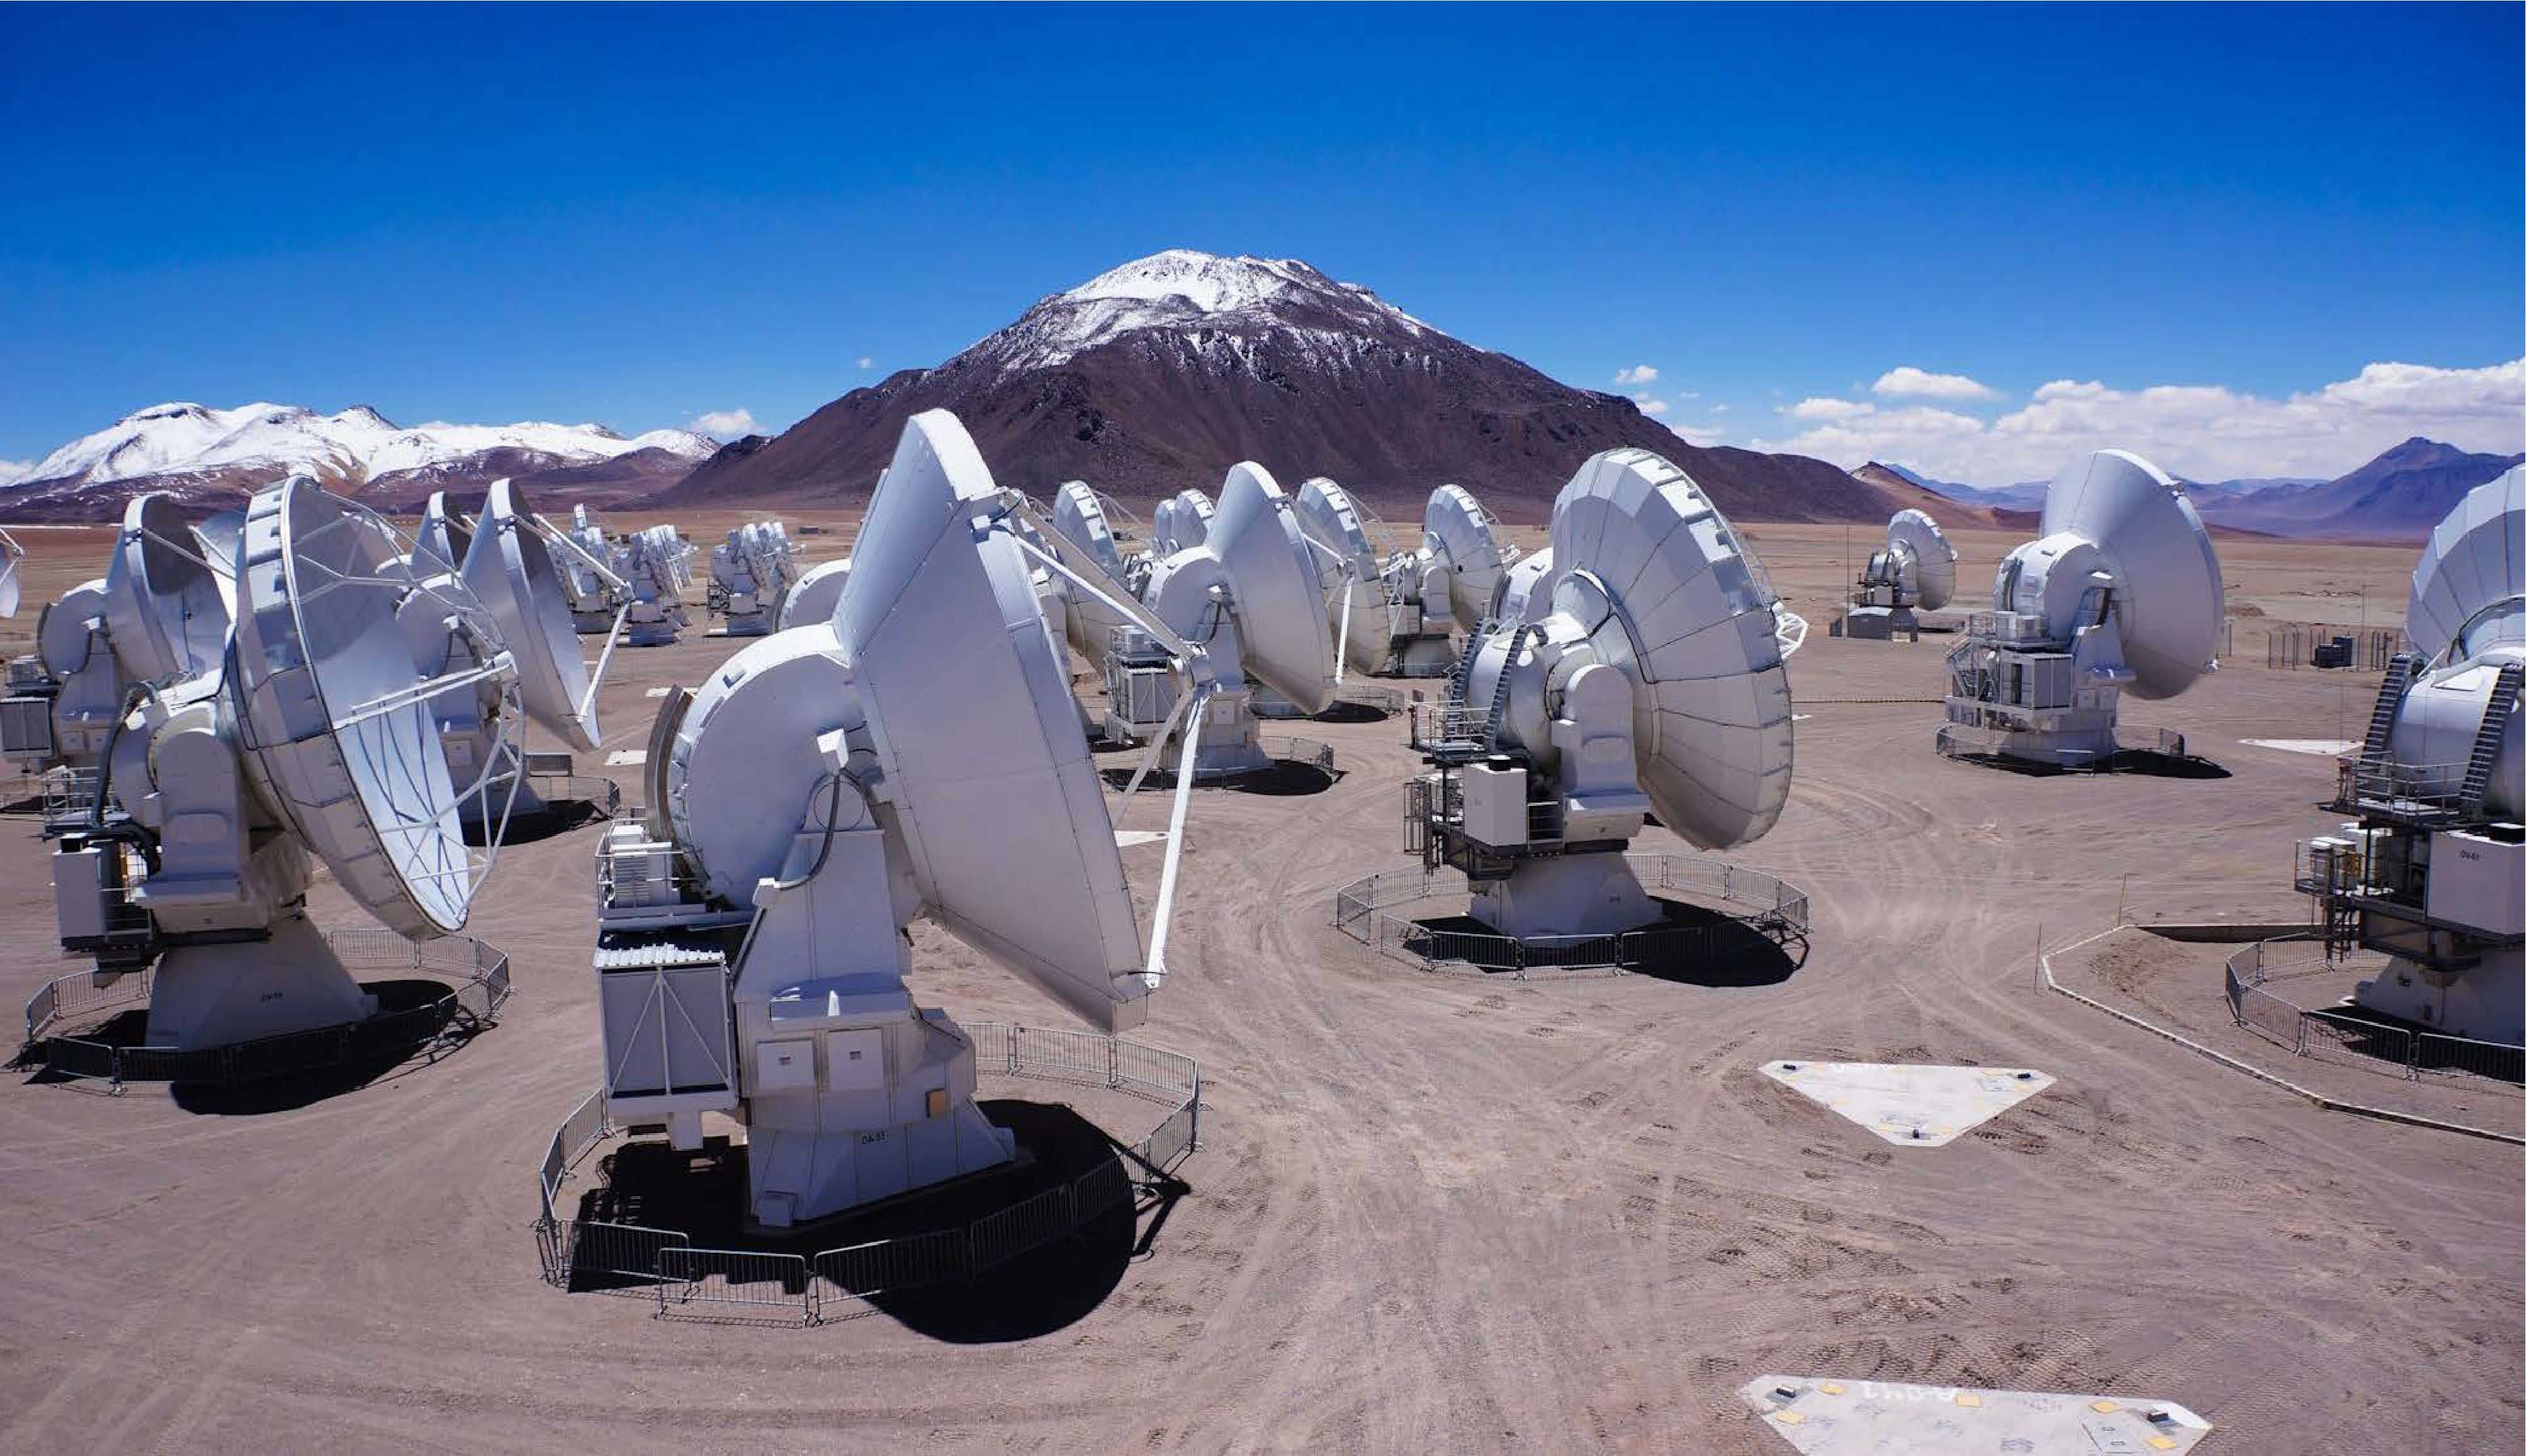
\includegraphics[width=\textwidth]{images/chapters/introduction/ism/ALMA_ACA_PCarrillo.pdf}
    \caption[Atacama Large Millimeter/Submillimeter Array]{View of the inner core of the Atacama Large Millimeter/Submillimeter Array (ALMA) on the Chajnantor plateau (Chile) with the Cerro El Chasc\`on (5703\,m) in the background. A total of 66 antennas ($12 \times 7$\,m diameter, $54 \times 12$\,m diameter) form the ALMA interferometer with baselines up to 16\,km. The combined collecting area allows for high sensitivity while the interferometer setup provides unprecedented resolution in the submillimeter wavelengths.
    Credit: NRAO, P. Carillo}
    \label{introduction: figure: ALMA}
\end{figure}

%%%%%%%%%%%%%%%%%%%%%%%%%%%%%%%%%%%%%%%%%%%%%%%%%%%%%%%%%%%%%%%%%%%%%%%%%%%%%%%%%%%%%%%%%%%%%%%%%%%%

%%%%%%%%%%%%%%%%%%%%%%%%%%%%%%%%%%%%%%%%%%%%%%%%%%%%%%%%%%%%%%%%%%%%%%%%%%%%%%%%%%%%%%%%%%%%%%%%%%%%

\chapter{Star formation and star forming galaxies}
\chaptermark{star formation}
\label{introduction: chapter: star formation}

%%%%%%%%%%%%%%%%%%%%%%%%%%%%%%%%%%%%%%%%%%%%%%%%%%%%%%%%%%%%%%%%%%%%%%%%%%%%%%%%%%%%%%%%%%%%%%%%%%%%

\section{Star formation in molecular clouds}
\label{introduction: section: star formation: SF in clouds}

\subsection{A sketch of the star formation process}
\label{introduction: section: star formation: sketch}

If the gravitational force of a molecular clouds mass overcomes potential stabilizing forces, the cloud will collapse to smaller size and higher density. In this process, the clouds usually fragments into cores that can collapse faster than the overall cloud.
Eventually, the collapsing pre-stellar core stabilizes due to radiation pressure of the beginning nuclear fusion but continues to accrete mass from the surrounding, still collapsing, cloud.
In massive clouds, enough mass is present for the formation of dozens to millions of stars which can remain bound in a stellar cluster or even super star cluster (Section~\ref{introduction: section: star formation: SSCs}). 

A newly formed proto-star is still embedded in the cloud from which it formed and it is therefore challenging to observe this phase of star formation. Infrared radiation from the cloud core and proto-star can escape the cloud but, especially for massive and dense clouds, longer wavelengths in the sub-mm regime subject to less extinction are required.
After its birth, a (proto-)star begins to dissociate and disperse its natal cloud through proto-stellar outflows and radiation (feedback, Section~\ref{introduction: section: star formation: feedback}) with the help of its siblings formed in the same cloud. 
The diverging size scales in star formation from stars (R$_\odot \sim 10^{-8}$\,pc) in cloud cores ($\LESSSIM$ pc) embedded in GMCs (up to $200$\,pc) that are influenced by galactic processes (several kpc) make it difficult to understand and model these early phases.


\subsection{Why is star formation inefficient?}
\label{introduction: section: star formation: inefficiency}

Of course, star formation is much more complicated than the simple sketch outlined above and many details of the star formation process are known today. However, there are still fundamental problems yet to be solved and understood in detail.
In the following, one important complex of problems is highlighted since they are related to this thesis.

\begin{figure}[t]
	\centering
	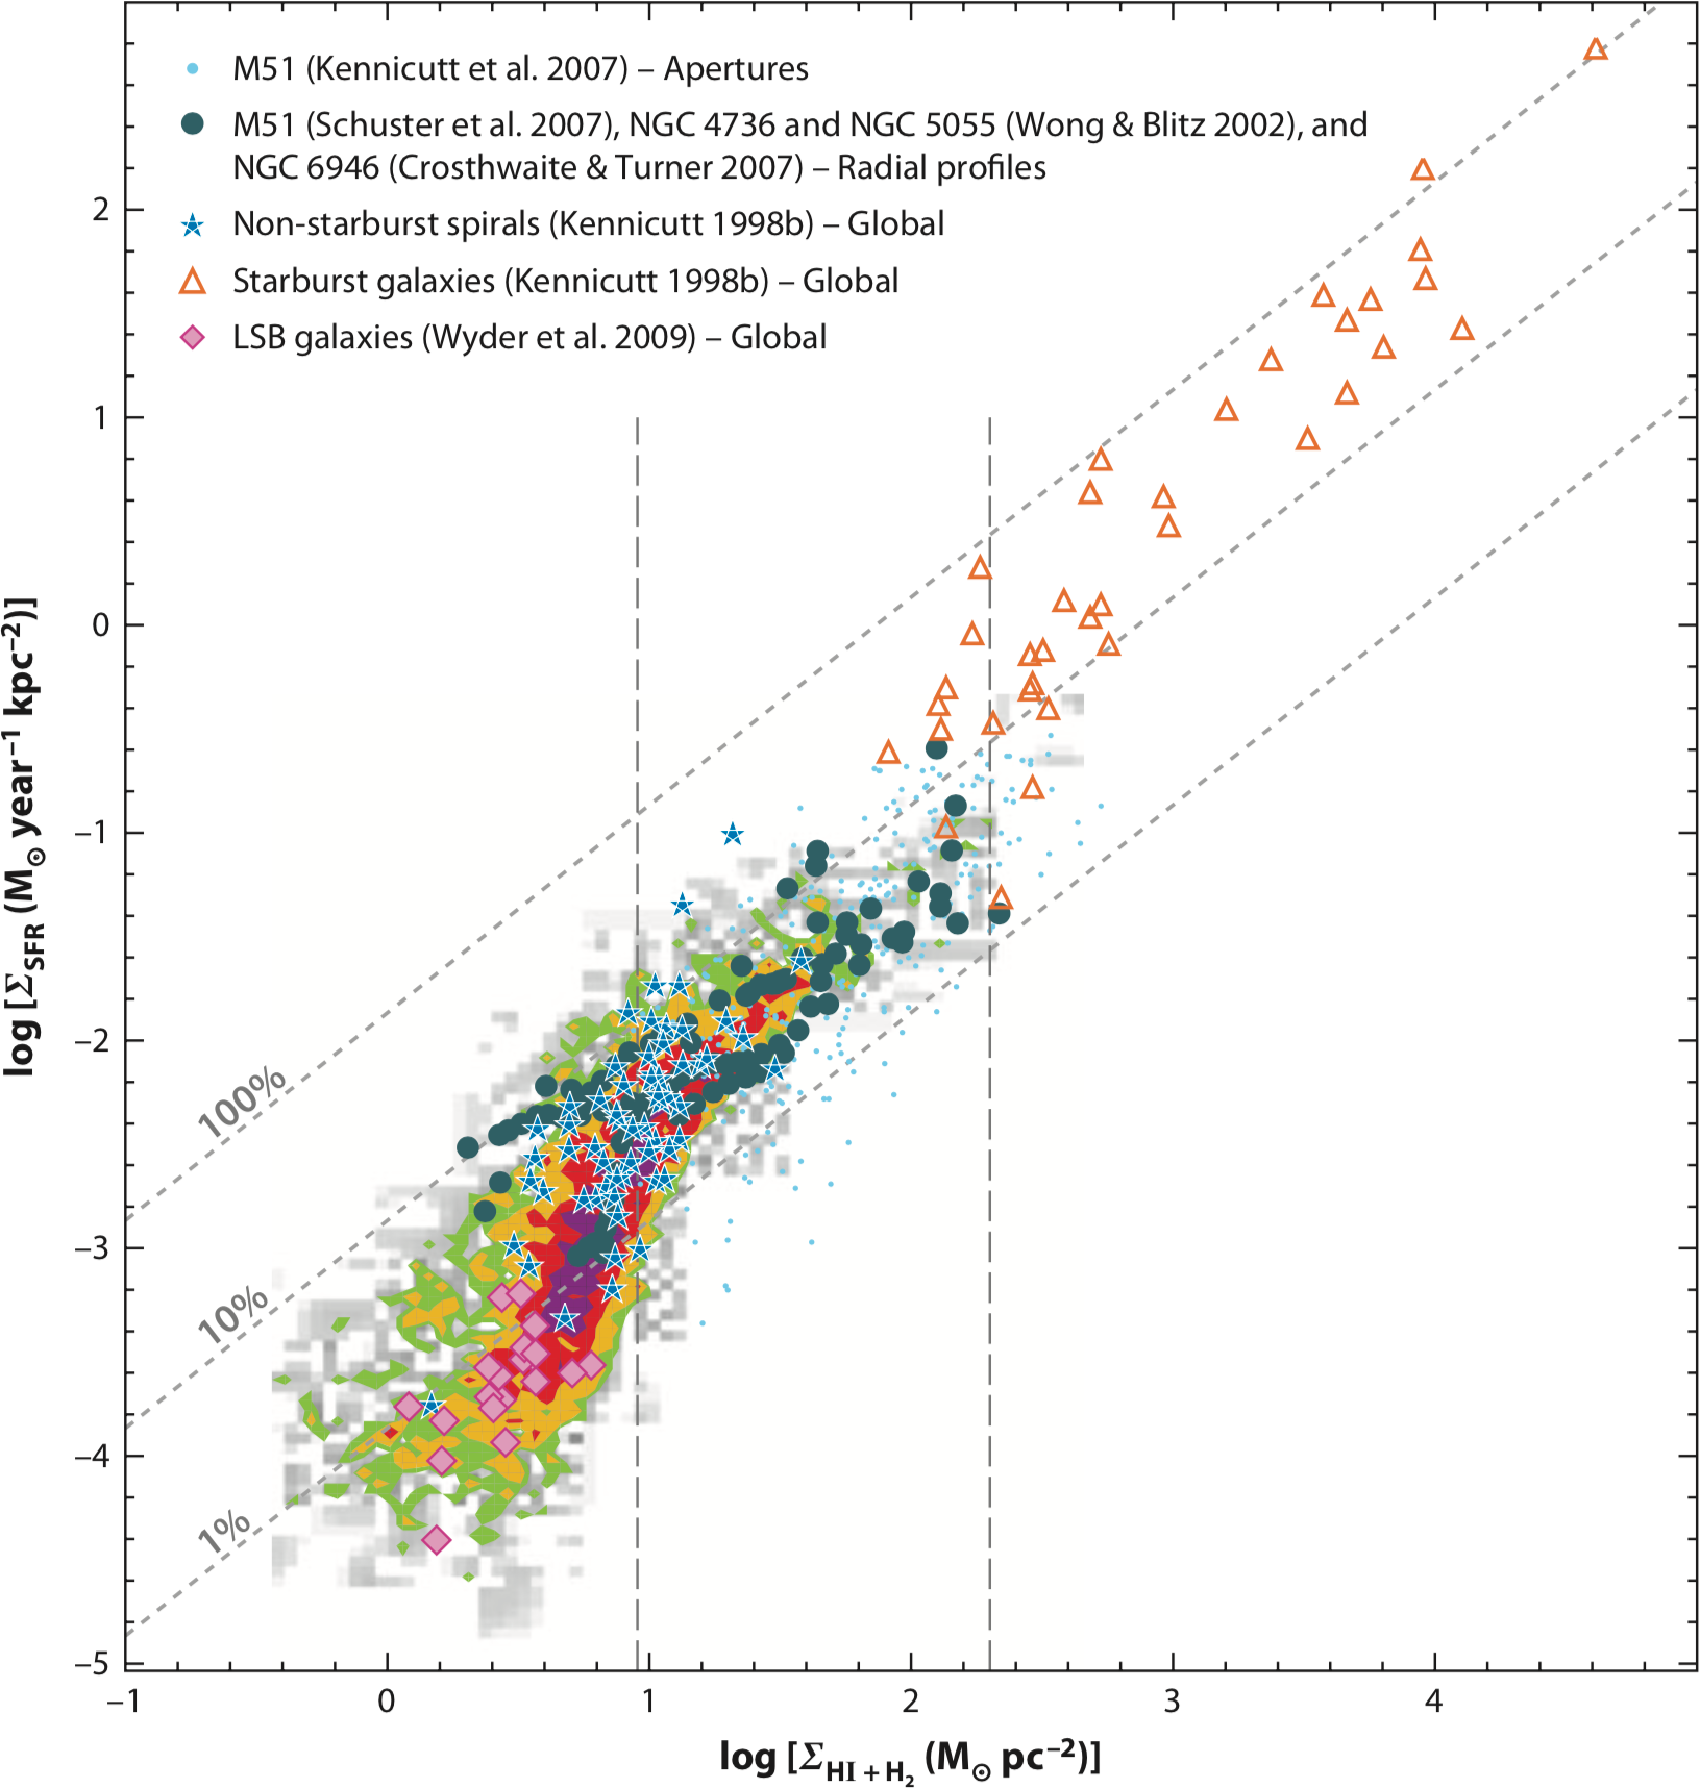
\includegraphics[width=0.8\linewidth]{images/chapters/introduction/sf/SF_law.pdf}
	\caption[Star formation (Kennicutt-Schmidt) law]{The star formation law (Kennicutt-Schmidt law) relates gas surface density to star formation rate surface density. In this figure from (\citealt{2012ARA&A..50..531K}; in original form in \citealt{2008AJ....136.2846B}) the total gas as the sum of neutral and molecular gas is shown. Typical star forming galaxies have low star formation efficiencies of up to a few percent depending on observational details (e.g. aperture size, location in the disk) while starbursts convert gas into stars much more efficiently.}
	\label{introduction: figure: star formation: SF law}
\end{figure}

Star formation seems extremely inefficient when comparing the amount of available gas to the ongoing star formation and the number of young stars \citep[e.g.][]{2007ARA&A..45..565M,2014PhR...539...49K}.
On the scale of galaxies or kpc sized regions within galaxies, the star formation law (Kennicut-Schmidt law) $\Sigma_{SFR} \propto \Sigma_{gas}^n$ quantifies the correlation between (molecular) gas and star formation \citep{1959ApJ...129..243S,Kennicutt:1998id}. It relates star formation rate surface density $\Sigma_{SFR}$ to molecular or total (molecular and neutral) gas mass surface density $\Sigma_{gas}$.
\citet{Kennicutt:1998id} found $n = 1.4 \pm 0.15$ for HI observations as the average over 100 nearby galaxies while \citet{1959ApJ...129..243S} originally suggested $n \sim2$. 
Figure~\ref{introduction: figure: star formation: SF law} shows a compilation of the literature for the total gas mass from \citet{2012ARA&A..50..531K}.

The ratio of gas mass available to star formation and the observed SFR (or equivalently the respective surface densities) defines the gas depletion time $\tau_\mathrm{dep} = M_\mathrm{mol}/SFR$. 
The inverse of the depletion time is the star formation efficiency $SFE = \tau_\mathrm{dep}^{-1}$ and describes how much and how fast gas is converted into stars.
The SF law is therefore tightly linked to the (in-)efficiency of star formation and suggests star formation efficiencies of $\sim 10^{-9}$\,Gyr$^{-1}$ (or $\tau_\mathrm{dep} \sim 1$\,Gyr) in typical star forming galaxies.

The (star forming) gas is characterized by the free-fall time $\tau_\mathrm{ff} = \sqrt{3\pi / 32 G \rho}$ that depends entirely on the gas density $\rho$ and describes the time required for the gas to collapse. Alternative formulations of the $SFE = SFR/M_\mathrm{mol}$ also consider this natural timescale (and/or other timescales) of molecular clouds.

The star formation efficiency $\epsilon_\mathrm{ff} = \tau_\mathrm{ff} / \tau_\mathrm{dep}$ eliminates the time dependence of the SFE \citep{2005ApJ...630..250K} and observations show a nearly universal efficiency of order 1\% \citep[e.g.][]{Krumholz:2012ja,2018ApJ...861L..18U,2017A&A...604A..74S}.

The solution to the efficiency problem is not yet entirely clear. Studies of star formation across various size scales show a scale dependence such that, although star formation is very inefficient on large scales, the smallest structures such as cloud cores can reach $30-70$\% \citep{2013ApJ...763...51F,2014prpl.conf...77P}. In the context of turbulence regulated star formation models, this shows how cores can collapse efficiently while stabilizing forces (primarily turbulence, but also magnetic fields) can prevent other regions within a cloud from forming stars \citep[e.g.][]{2019ApJ...883....2S}.

Stellar feedback (Section~\ref{introduction: section: star formation: feedback}) is known to play an important role in generating turbulence, but other dynamical effects (e.g. magneto-rotational instability, accretion driven) on galactic scales contribute to the generation of turbulence\citep[e.g.][]{2019ApJ...871...17U}.
However, it is not yet understood how stellar feedback couples to the star forming gas to drive turbulence. One manifestation of feedback are outflows which could not yet be studied in detail (meaning at high spatial resolution on pc scales), a problem that this thesis addresses.

Figure~\ref{introduction: figure: star formation: SF law} also shows that starburst galaxies (Section~\ref{introdution: section: star formation: starbursts}) achieve much higher SFE than typical star forming galaxies. The path to a unified model of star formation therefore must include the study of starbursts. It needs to be better understood how exactly starbursts differ from other galaxies in their gas and star forming properties. This thesis presents important steps towards that goal by studying a particular starburst at highest resolution.


%%%%%%%%%%%%%%%%%%%%%%%%%%%%%%%%%%%%%%%%%%%%%%%%%%%%%%%%%%%%%%%%%%%%%%%%%%%%%%%%%%%%%%%%%%%%%%%%%%%%

\section{Super star clusters}
\label{introduction: section: star formation: SSCs}

\begin{figure}[t]
	\centering
	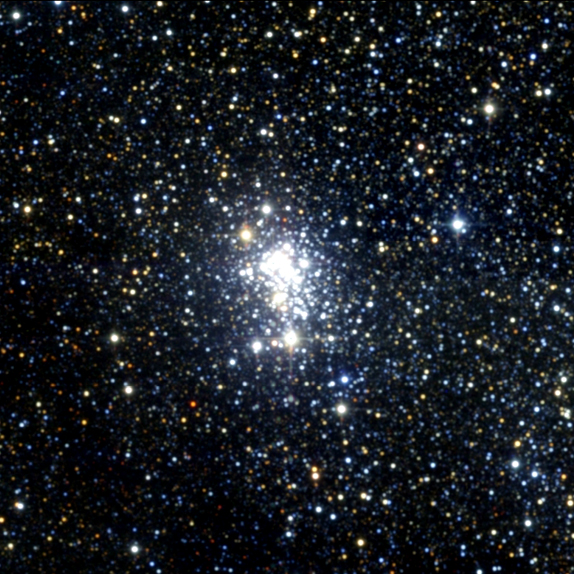
\includegraphics[width=0.6\linewidth]{images/chapters/introduction/sf/westerlund1_IR.jpg}
	\caption[Super star cluster Westerlund 1]{The super star cluster Westerlund~1 in the infrared as seen by the 2 Micron All-Sky Survey (2MASS). Westerlund~1 with a mass of $M_\ast \sim 6\times10^4$\,\Msun was the first SSC discovered in the Milky Way. Credit: 2MASS/UMass/IPAC-Caltech/NASA/NSF.}
	\label{introduction: figure: star formation: SSC example}
\end{figure}

For very massive molecular clouds, the product of the star formation process can be an also very massive stellar cluster, e.g. Arches \citep[$M_\ast = 10^{4.3}$\,\Msun;][]{1999ApJ...514..202F} and Quintuplet \citep[$M_\ast = 10^{4.0}$\,\Msun;][]{2006ApJ...643.1166F} in the Milky Way Galactic center or R136 in the Large Magellanic Cloud \citep[$M_\ast = 10^{4.78}$\,\Msun; e.g.][]{1995ApJ...448..179H,2009ApJ...707.1347A}.
Even more massive clusters can be found outside the local group and go by the name super star clusters (SSCs). The distinction from other stellar clusters is somewhat arbitrary and usually defined to cover the most massive ($M \GTR 10^5$\,\Msun) and very compact ($R \sim 1$\,pc) systems. SSCs are especially prevalent in starbursts like M82 or the antennae \citep[e.g.][]{2005ApJ...621..278M,2003dhst.symp..153W,2015ApJ...806...35J}.

SSCs are thought to be younger cousins of globular clusters \citep[e.g.][]{2015IJMPD..2430002B} and might thus help to understand the formation of old stellar systems and the evolution of galaxies (also see Section~\ref{introduction: section: star formation: cosmological context}). Globular clusters are massive ($M \GTR 10^5$\,\Msun), compact ($R \sim 10$\,pc) and very old ($\GTR 10$\,Gyr). Taking evolutionary effects (late-phase stellar mass loss, stars evaporating off the cluster, tidal interactions) into account, globular clusters must have formed with very high masses $M \GTRSIM 10^6$\,\Msun, similar to the most massive SSCs in the local universe.

To date, SSCs have been found in $\GTR20$ nearby galaxies including \ngc253 \citep{Watson:1996dn,Kornei:2009ee}, ESO338 \citep{2007A&A...461..471O}, \ngc5253 \citep{2017ApJ...846...73T}, M51 and M82 (see the review by \citealt{2010ARA&A..48..431P} for an overview).
Very young and still forming SSCs have been found in the Antennae \citep{2012A&A...538L...9H,2015ApJ...806...35J}, the Large Magellanic Cloud \citep{2017NatAs...1..784O}, \ngc253 \citep{2018ApJ...869..126L} and \ngc5253 \citep{2017ApJ...846...73T}. The high extinction of the large amounts of dense gas obscures potential young clusters and only recently it became possible to resolve SSC scales with ALMA in the less affected sub-mm wavelengths.
Chapter~\ref{chapter: SSCs} presents a study of the physical and chemical properties of the ISM in and around young (proto-)SSCs in \ngc253 with resolved observations for the first time.


%%%%%%%%%%%%%%%%%%%%%%%%%%%%%%%%%%%%%%%%%%%%%%%%%%%%%%%%%%%%%%%%%%%%%%%%%%%%%%%%%%%%%%%%%%%%%%%%%%%%

\section{The main sequence of star forming galaxies}
\label{introduction: section: star formation: main sequence}

Galaxies can be empirically grouped into different classes according to their location in the plane of star formation rate versus stellar mass (Figure~\ref{introduction: figure: star formation: MS}).
Galaxies of typically blue color are found to lie on a diagonal sequence, i.e. their star formation rate scales with stellar mass \citep[e.g.][]{2004MNRAS.351.1151B,2011A&A...533A.119E}. This relation is called the main sequence (MS) of star forming galaxies (SFGs).
Most other galaxies are located in a clumpy structure at low star formation rates nearly independent of stellar mass. Since these galaxies are passive and typically red in color, they are called red clump galaxies, or ``red and dead'' in colloquial terms.
Galaxies in the transition region are far more sparse and thus denoted green valley galaxies because they lie in between the peaks of red and blue galaxies.

\begin{figure}[t]
	\centering
	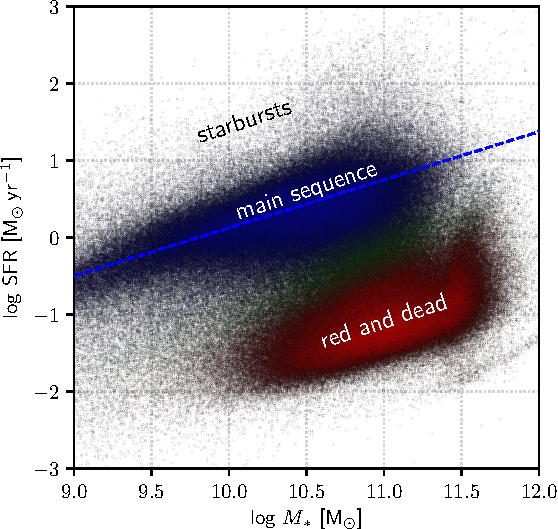
\includegraphics[width=0.6\linewidth]{images/chapters/introduction/sf/SDSS_main_sequence.pdf}
	\caption[Main sequence of star forming galaxies]{About 270,000 galaxies from SDSS DR8 sample the parameter space in the stellar mass vs. star formation rate plane and reveal a galaxy bimodality. The main sequence of star forming galaxies is an empirical relation on which typical starforming galaxies fall. Galaxies above the relation are called starbursts. Old, red, typically elliptical galaxies fall below the main sequence and after often referred to as ``red and dead''. The green valley is a name given to the transition region between starforming main sequence and quiescent red and dead galaxies.}
	\label{introduction: figure: star formation: MS}
\end{figure}

A single galaxy is not static in the stellar mass -- star formation rate diagram but can evolve through the different phases \citep[e.g.][]{2006MNRAS.368....2D,2018MNRAS.474.2039E}. Mergers or gas infall can trigger star formation and push the galaxy up into the starburst regime. When the gas is eventually consumed by star formation or has become unavailable to star formation by other processes, the galaxy moves down the diagram through the green valley to become a passive galaxy.

The position in the stellar mass -- star formation rate diagram correlates with galaxy morphology \citep[e.g.][]{2004MNRAS.351.1151B}. Red clump galaxies are typically elliptical (early Hubble types) while main sequence and starbursts are typically spirals (late Hubble types). Starburst galaxies are also often irregular in shape.


%%%%%%%%%%%%%%%%%%%%%%%%%%%%%%%%%%%%%%%%%%%%%%%%%%%%%%%%%%%%%%%%%%%%%%%%%%%%%%%%%%%%%%%%%%%%%%%%%%%%

\section{Starbursts}
\label{introdution: section: star formation: starbursts}

Starbursts are located above the MS at increased star formation rates. The distinction between MS and starbursts is based on the depletion time (Section~\ref{introduction: section: star formation: inefficiency}) of the molecular gas reservoir under the observed star formation rate. As mentioned before, normal star forming galaxies have typical depletion times $\tau_\mathrm{dep} \sim 1-2$\,Gyr \citep[e.g.][]{Leroy:2008jk} whereas starbursts consume their molecular gas at a much higher rate in $\tau_\mathrm{dep} \sim 0.1$\,Gyr \citep[e.g.][]{Kennicutt:1998id,2008AJ....136.2846B}.
The transition from MS to starburst is fluent and not coupled to a specific depletion time. Instead, the strength of a starburst can be parametrized as the offset from the MS.

\begin{figure}
	\centering
	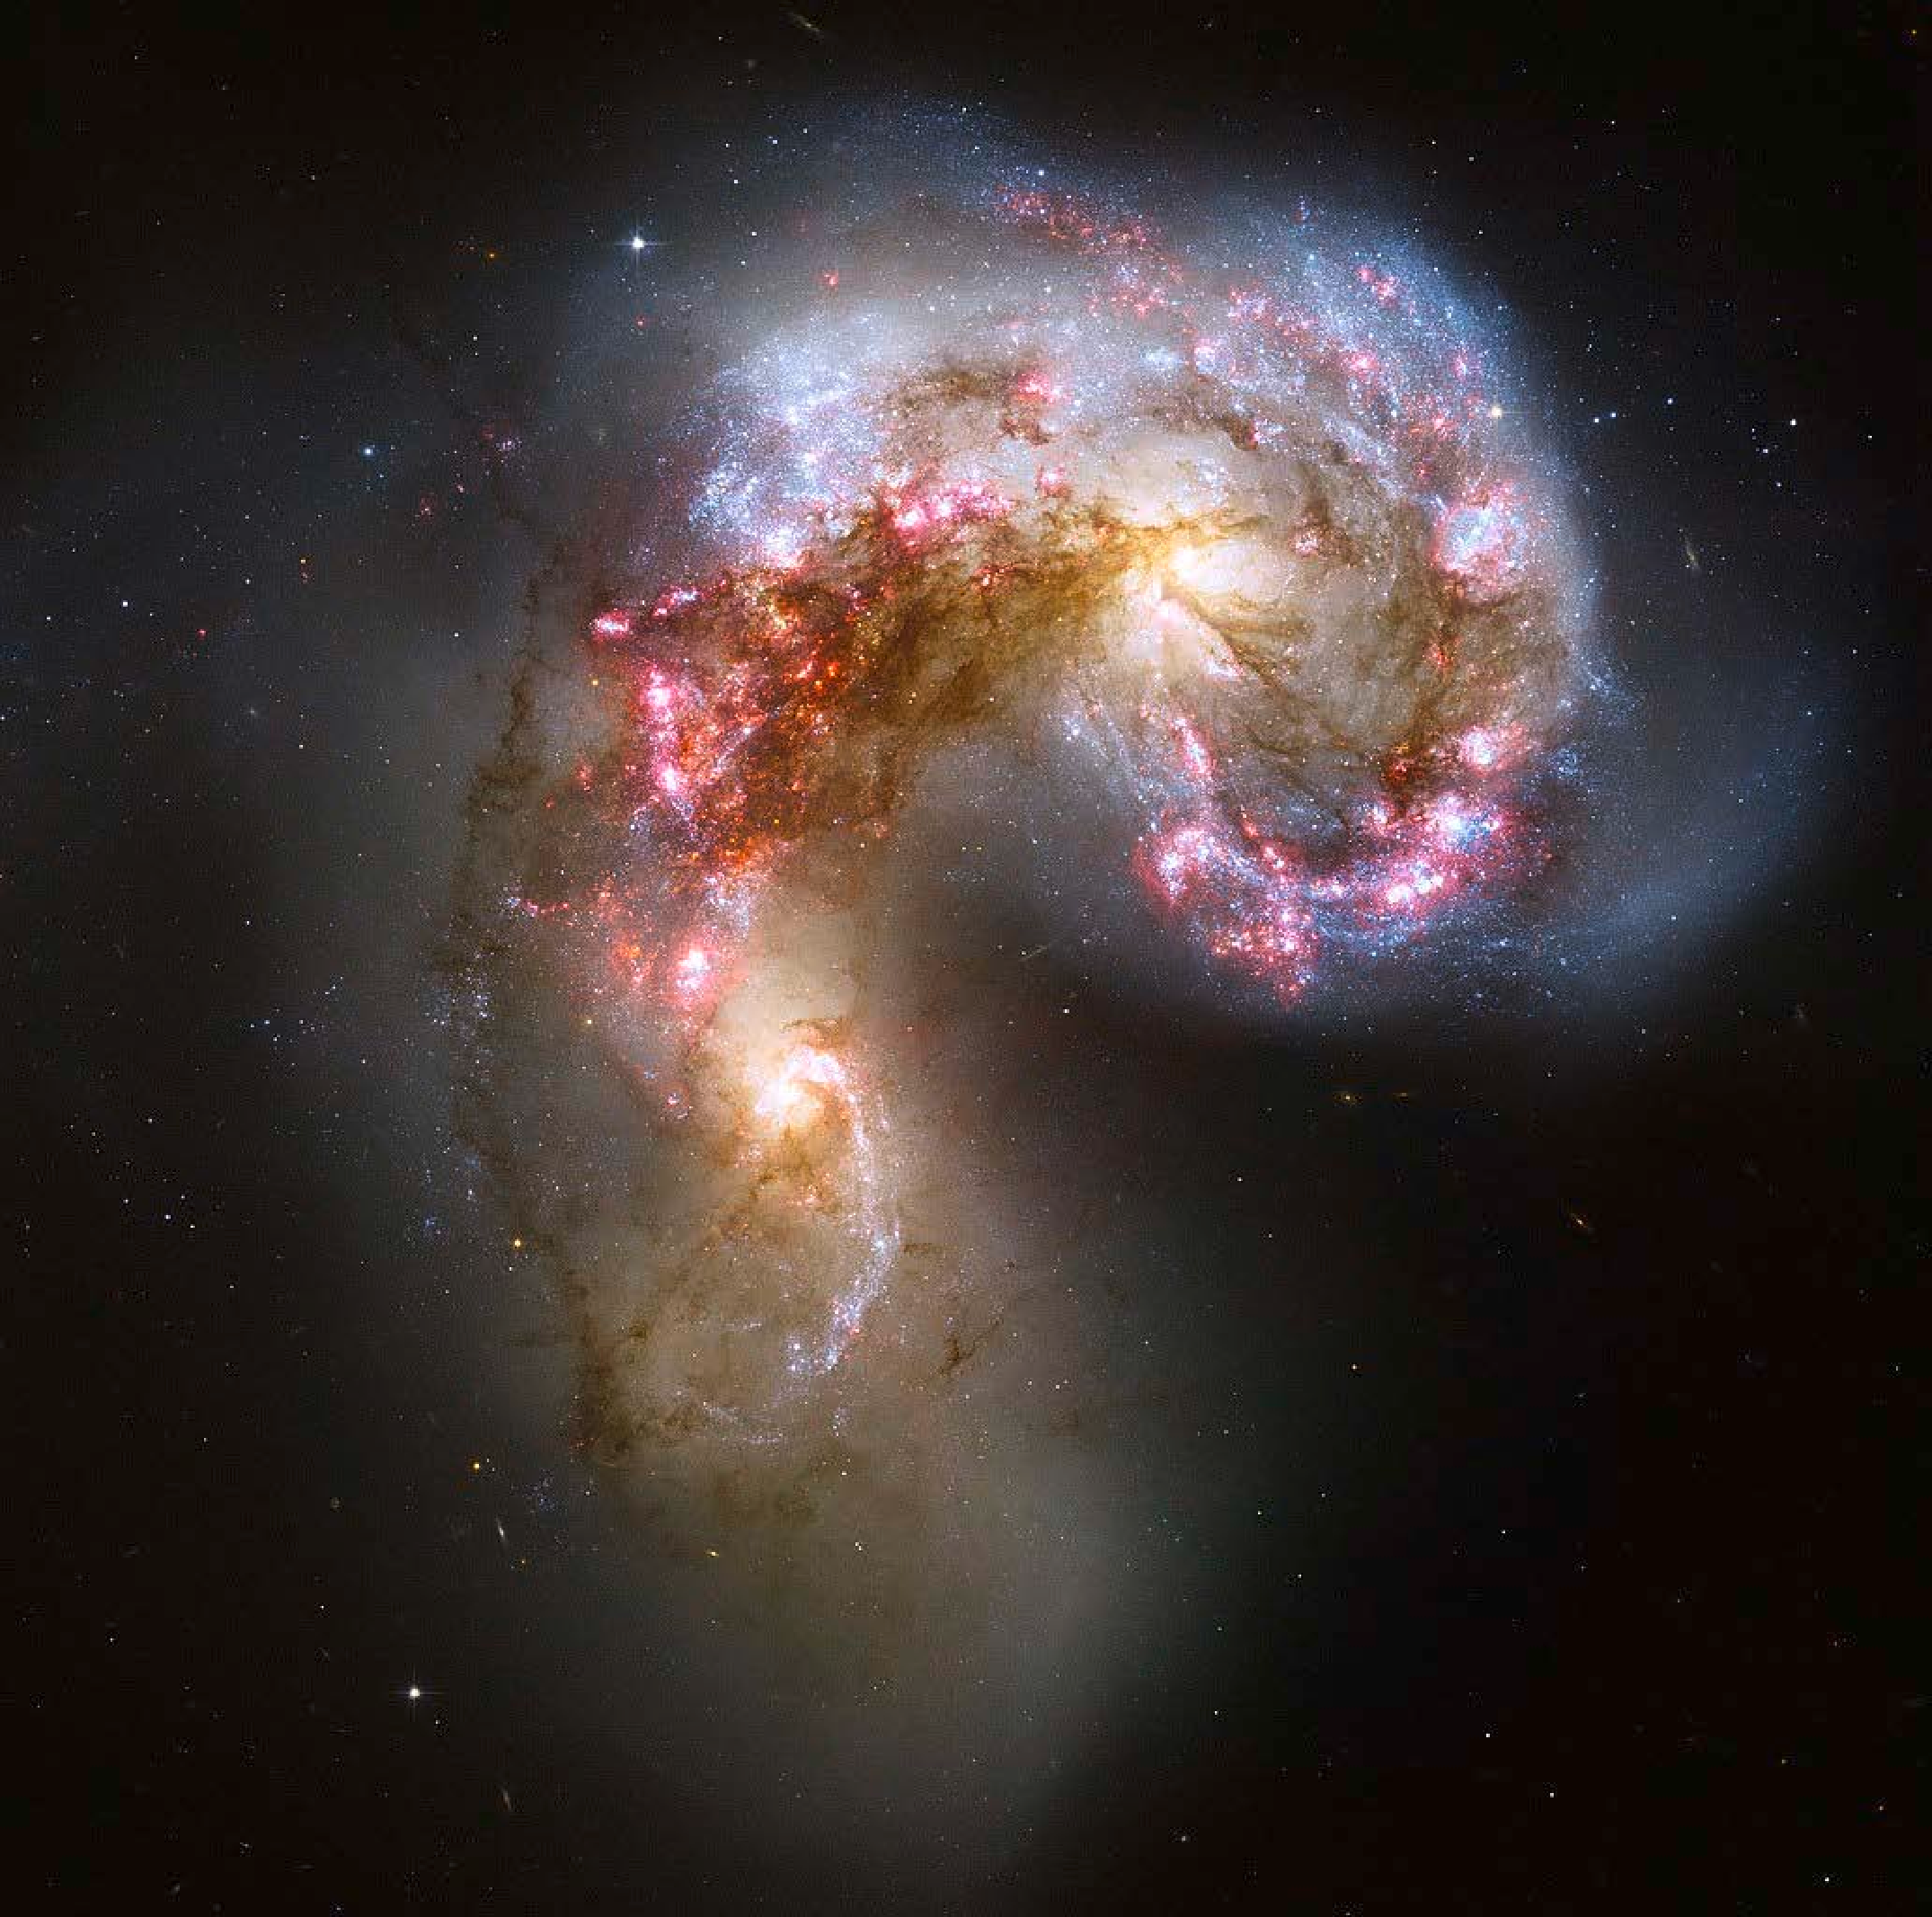
\includegraphics[width=\linewidth]{images/chapters/introduction/sf/Antennae_HST.pdf}
	\caption[Starburst in the Antennae galaxies]{The Antennae galaxies are a proto-typical example of a starburst driven by the tidal interaction and merging of galaxies. The brightest star forming regions host young and forming super star clusters. Source: HST press release \href{https://www.spacetelescope.org/news/heic0615/}{heic0615}.}
	\label{introduction: figure: star formation: Antennae starburst}
\end{figure}

Starbursts can encompass a whole galaxy or just parts thereof, typically, the center. It can be triggered in multiple ways through dynamical forces either by increasing the availability of dense gas or increasing the star formation efficiency \citep[e.g.][]{1991ApJ...370L..65B,1992ARA&A..30..705B}.

The gravitational interaction with other galaxies in major or minor mergers can shock and compress gas which increases the density, allows hot/warm gas to cool and can lead to the formation of dense molecular gas. Tidal forces during the interaction can redistribute angular momentum and drive (molecular) gas to the galaxies' centers where it accumulates to fuel enhanced star formation \citep[e.g.][]{1996ApJ...464..641M}. The Antennae galaxies shown in Figure~\ref{introduction: figure: star formation: Antennae starburst} are an example for a merger or interaction triggered starburst.

Hydrodynamic instabilities in the gas disk of a galaxy can lead to the accumulation of dense gas and therefore enhanced SFR. A typical example are bar instabilities that allow for an efficient transfer of mass into a galaxy's center \citep[e.g.][]{2004ARA&A..42..603K} as is the case in \ngc253 \citep{2000PASJ...52..785S}.
Even if the inflow rate towards the galactic center is not high enough to sustain such a bar-driven starburst, it may be sufficient to ignite periodic short starbursts when the accumulated mass exceeds local limits as is discussed for the Galactic center \citep[e.g.][]{2015MNRAS.453..739K}.


%%%%%%%%%%%%%%%%%%%%%%%%%%%%%%%%%%%%%%%%%%%%%%%%%%%%%%%%%%%%%%%%%%%%%%%%%%%%%%%%%%%%%%%%%%%%%%%%%%%%

\section{Star formation feedback}
\label{introduction: section: star formation: feedback}

\subsection{Mechanisms}
Stars, especially high-mass stars, emit significant amounts of mass, energy and momentum into their surroundings. The combined effect on the ISM is called stellar feedback \citep[e.g.][]{1987ARA&A..25...23S}.
Even before having formed a main sequence star, proto-stellar objects launch gas into their surrounding on stellar ($\LESSSIM$\,pc) scales while accreting from their proto-stellar disk \citep[e.g.][]{1995ApJS..101..117K}.
Once on the stellar main sequence, the fusion processes scale with the stellar mass which causes more massive stars to undergo an increasingly rapid evolution. Hot ($T \GTRSIM 10^4$\,K), young (few Myr) and massive ($M \GTRSIM 3$\,\Msun) O- and B-type stars are violently burning hydrogen and produce intense UV radiation that exerts pressure on the surrounding ISM \citep[e.g.][]{1955ApJ...121....6O,1995ApJ...455..269L}.
Later in the evolution, red giants and supergiants on the asymptotic giant branch (AGB) launch intense, massive stellar winds driven by radiation pressure on the marginally bound outer layers of the stellar atmosphere \citep[e.g.][]{2001A&A...369..574V}. 

Aside from stellar winds, supernovae (SN) are the other important feedback source from evolved stars.
The most massive stars beyond $M \GTR 8$\,\Msun end their life as a core-collapse supernova \citep[SN type II; e.g.][]{1995ApJS..101..181W}. The stellar core eventually reaches temperatures and densities high enough for electrons to combine with protons into neutrons and the electron degeneracy pressure suddenly drops and cannot aid to stabilize the core against gravitational collapse. The implosion of the star then rebounds on the formed neutron core and releases enormous amounts of energy into the stellar envelope that is blown off the star. Typically, only $\sim 20$\% of the pre-SN stellar mass ends up in the remnant meaning that $\sim 80$\% of the mass is ejected, even more when considering the mass loss by stellar winds earlier in the evolution.
Type Ia supernovae occur when an accreting white dwarf crosses the Chandrasekhar mass limit at $M \sim 1.4$\,\Msun and gravitation suddenly dominates over electron degeneracy pressure to trigger collapse and subsequent explosion \citep{1931ApJ....74...81C}.

The kinetic energy ($E \GTRSIM 10^{51}$\,erg) and momentum ($P \GTRSIM 3\times 10^4$\,\Msunyr\,\kms) released by SNe are enormous \citep[e.g.][]{Leitherer:1999jt}.
For a single event, supernovae easily dominate over the other forms of stellar feedback but the sparsity of supernovae ($\sim1$ per 100\,yr for a $SFR \sim 1$\,\Msunyr) limits their impact. In fact, stellar winds and supernovae contribute about equally to the released kinetic energy and momentum of stars \citep[e.g.][]{Leitherer:1999jt}.

For completeness, it needs to be noted that active galactic nuclei (AGN) can also exert feedback on the ISM. Depending on the environment, AGN feedback can add an additional feedback source or completely dominate over stellar feedback.
However, AGN feedback is not relevant for this thesis, so we omit it here.

\subsection{Effect on clouds}
The effect of stellar feedback on the ISM and star formation can be negative (i.e. prevent further star formation), positive (i.e. enhance star formation) or both.
After the first stars have formed in a cloud, their radiation will eventually dissociate, ionize and disperse the remaining (molecular) gas and limit further star formation \citep{2002ApJ...566..302M,2016MNRAS.463.3129G,2018ApJ...853..173K,2018MNRAS.481.2548G}. As such, feedback directly negatively effects the star formation locally by reducing the star formation efficiency of a cloud.
Furthermore, feedback introduces turbulent energy into the ISM that can help to stabilize molecular clouds against gravitational collapse in a state of quasi-static equilibrium \citep{2005ApJ...630..250K,2007ApJ...654..304K,2013ApJ...763...51F}. As such it can provide a preventive feedback loop in the star formation process. The relevant mechanisms are likely proto-stellar outflows on clouds scales \citep[e.g.][]{2010ApJ...709...27W,Krumholz:2012ja,2013A&A...558A..81B} and supernovae on larger up to galactic scales \citep{2016ApJ...822...11P}. It is still debated how much of the released energy and momentum is effectively deposited into the molecular clouds and thus how effective this negative feedback is \citep[e.g.][]{2010ApJ...715.1170A,2015Natur.527...70P,2018ApJ...855...81S}.

On the other hand, feedback creates shocks and (converging) gas flows that can locally enhance the density and enforce self-gravitation of otherwise stable clouds \citep[e.g.][]{1994A&A...290..421W,2012ApJ...744..130K}. Hence, a cloud may obtain more mass from the surrounding ISM that is then converted to stellar mass or it may only be able to become at all self-gravitating by the extra push from feedback. While plausible, the effectiveness of this positive feedback mode is debated \citep[e.g.][]{2015MNRAS.450.1199D,2017MNRAS.464.3536R} and discussed primarily for high redshift AGN feedback \citep[e.g.][]{2015ApJ...799...82C}.
Simulations suggest that both positive and negative feedback may occur side by side in a Galaxy depending on the exact conditions such as gas density and feedback strength \citep[e.g.][]{2017MNRAS.467..512S}


\begin{figure}
	\centering
	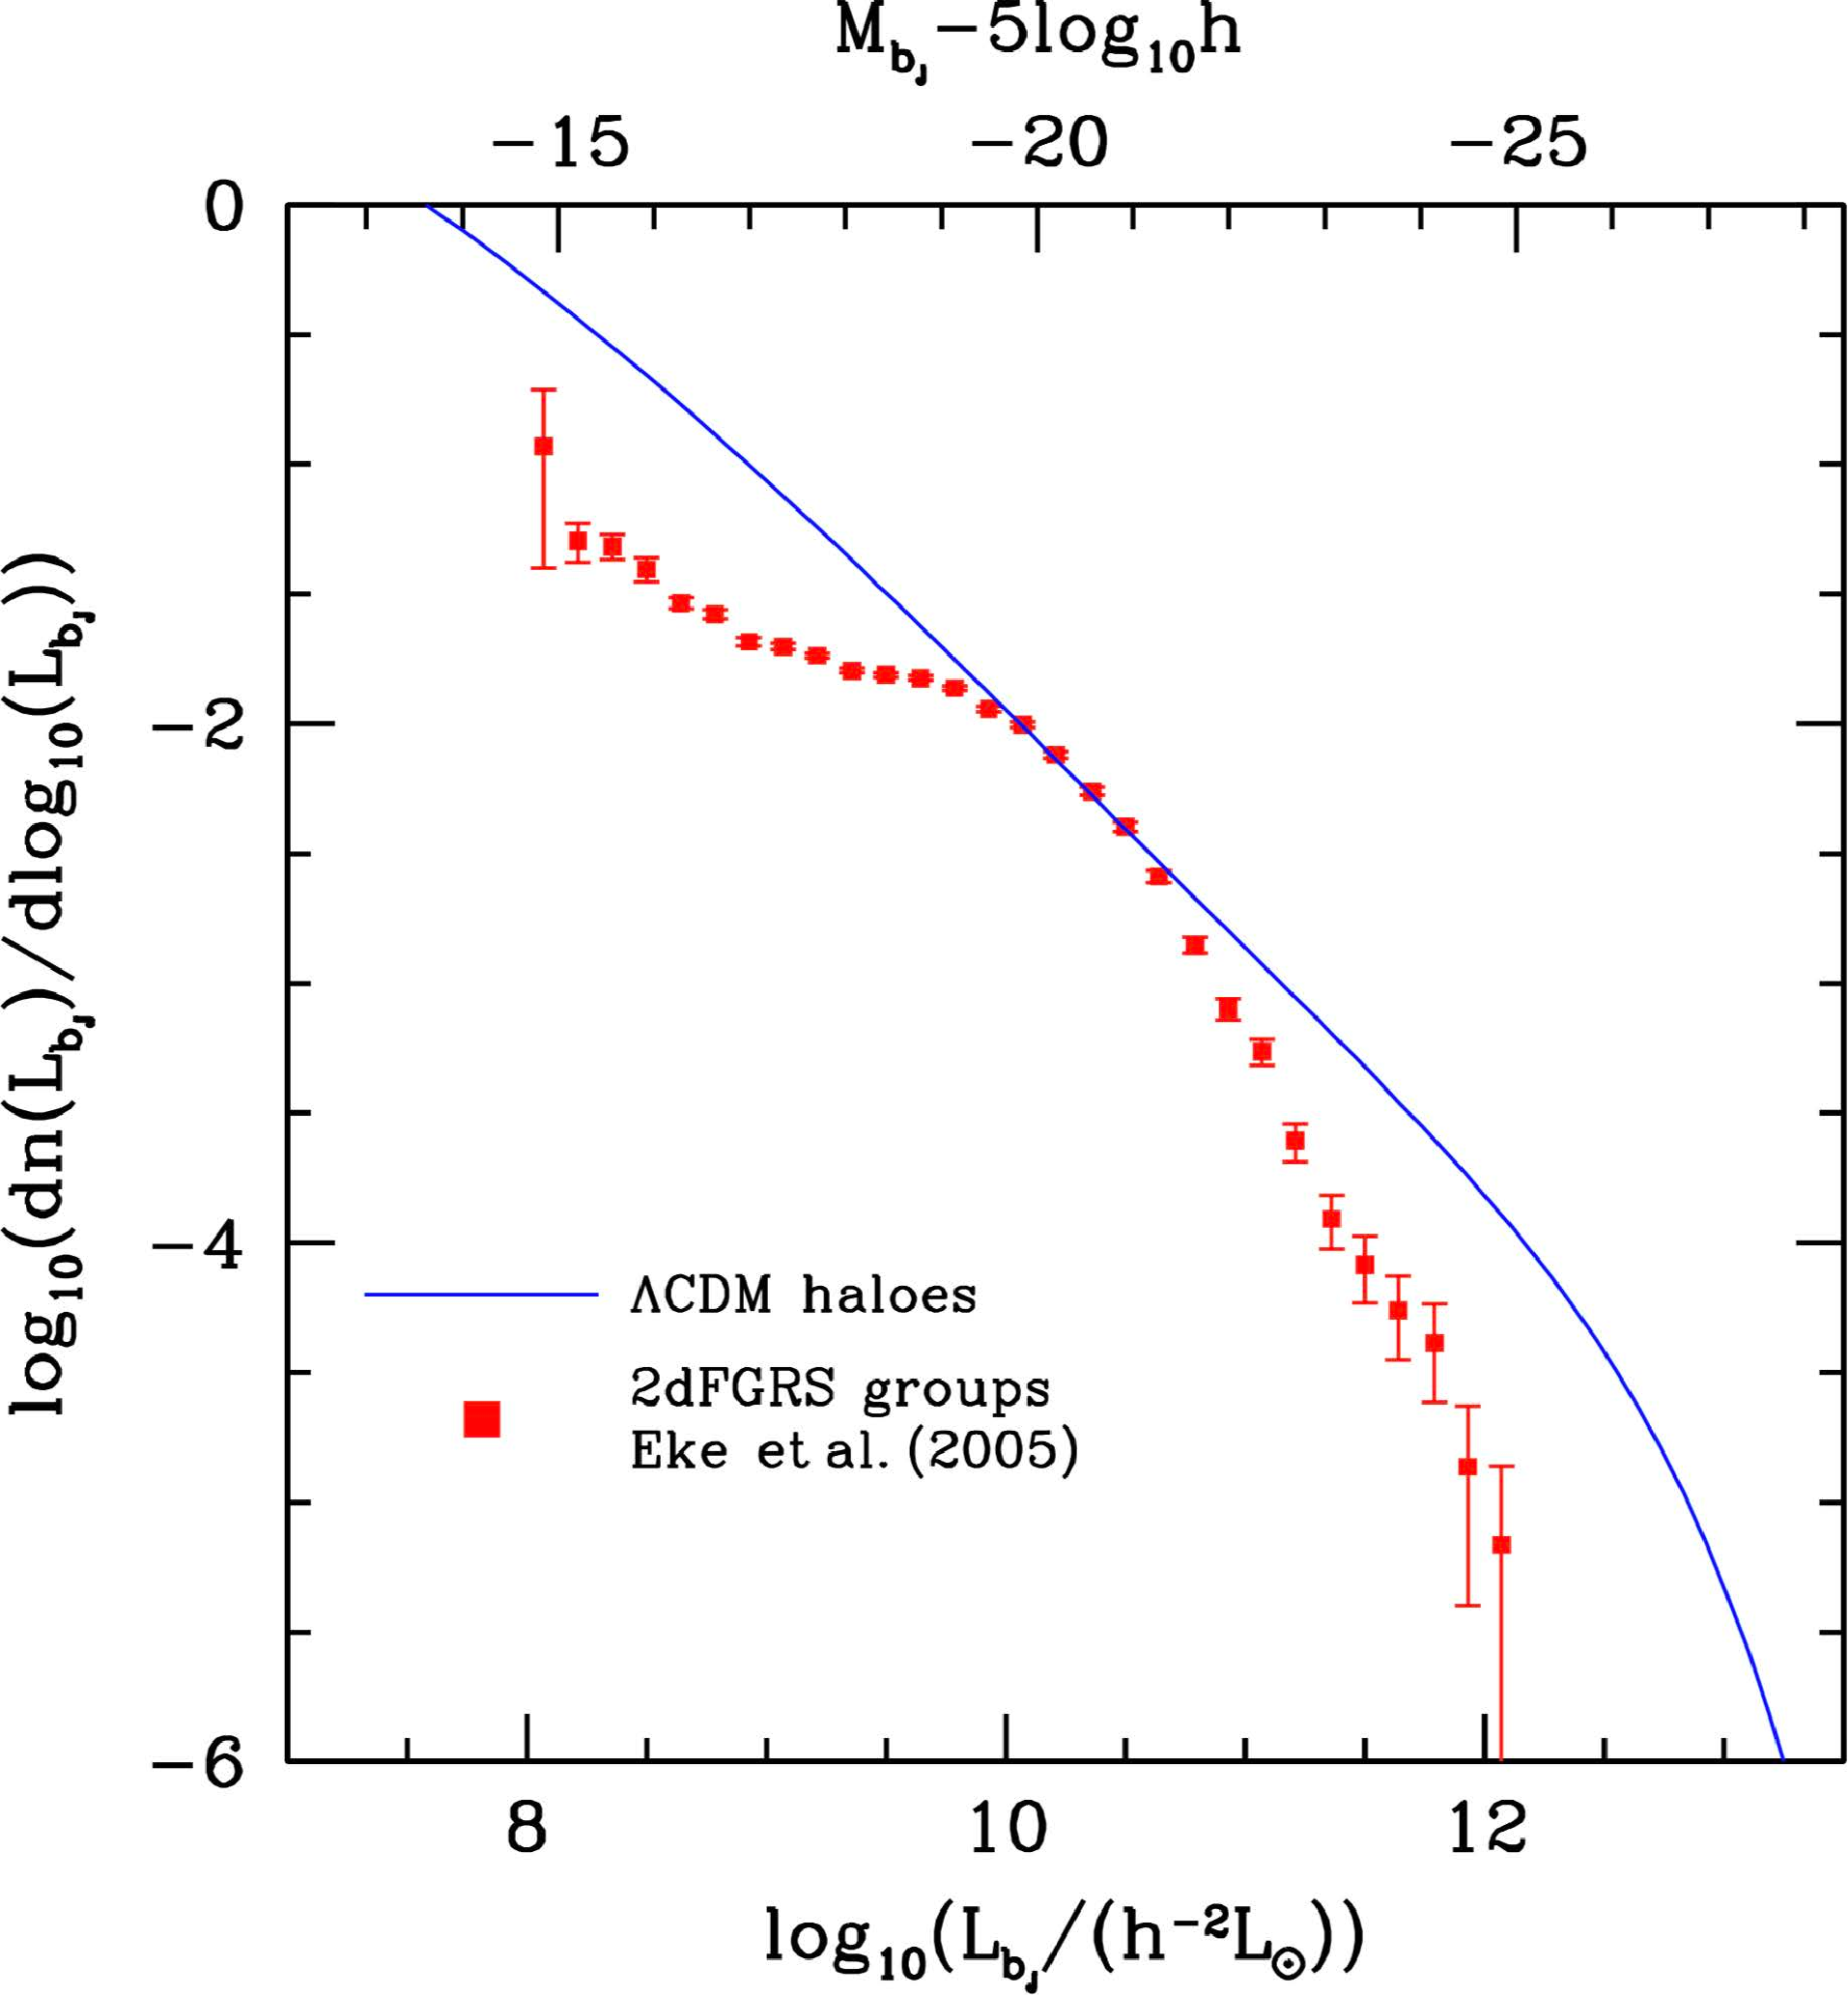
\includegraphics[width=0.55\linewidth]{images/chapters/introduction/sf/luminosity_function.pdf}
	\caption[Galaxy luminosity function compared to the $\Lambda$CDM prediction]{Comparison of the measured galaxy luminosity function (red) to the relation predicted by pure $\Lambda$CDM cosmology (blue). The luminosity function gives the normalized number of galaxies ($n$) as a function of galaxy bolometric luminosity ($L_b$). The mismatch between observations and simple $\Lambda$CDM models at high and low luminosities can be explained by AGN and stellar feedback, respectively. In the lower gravitational potential of dwarf galaxies (low luminosities), supernovae can effectively remove gas by launching outflows and thus suppress the buildup of stellar mass. High-mass galaxies are typically found at the centers of galaxy clusters where frequent interactions funnel gas to the centers resulting in AGN feedback and the shutdown of star formation.
	Figure taken from \citet{2006RPPh...69.3101B}.}
	\label{introduction: figure: star formation: luminosity function}
\end{figure}

\subsection{Effect on galaxies}
Feedback (stellar and AGN) must play a significant role in the formation and evolution of galaxies in the universe. Cosmological simulations not including feedback overpredict the amount of low-mass (low luminosity) but also high-mass (high luminosity) galaxies \citep[e.g.][]{2010gfe..book.....M,2013ApJ...770...57B}. The cosmological standard model $\Lambda$CDM predicts a power law form of the cosmic galaxy luminosity function which is not observed as shown in Figure~\ref{introduction: figure: star formation: luminosity function}. The inclusion of feedback into the models resolve this mismatch. At the low mass end, stellar feedback reduces the number of galaxies by removing gas from the galaxies that is lost for the built-up of stellar mass \citep[e.g.][]{1991ApJ...381...14L,2002MNRAS.330..113K}. At the high mass end, AGNs are increasingly common and thus AGN feedback that inhibits further star formation \citep[e.g.][]{2005MNRAS.361..776S,2006MNRAS.370..645B}.


%%%%%%%%%%%%%%%%%%%%%%%%%%%%%%%%%%%%%%%%%%%%%%%%%%%%%%%%%%%%%%%%%%%%%%%%%%%%%%%%%%%%%%%%%%%%%%%%%%%%

\section{Galactic outflows}
\label{introduction: section: star formation: outflows}

Strong stellar feedback caused by high star formation rate densities can launch outflows of ionized, neutral and molecular gas (Figure~\ref{introduction: figure: star formation: M82 outflow}) that potentially can escape the main body of a galaxy \citep[e.g.][]{1985Natur.317...44C}. Consequently, such outflowing gas removes the potential fuel for future star formation. Therefore, outflows can suppress and quench star formation, as also demonstrated by theoretical predictions and simulations \citep[e.g.][]{1986ApJ...303...39D,2017MNRAS.466.1213K,2018ApJ...857..116M}. Depending on the velocity of the outflow and a galaxy's escape velocity, outflowing gas can be re--accreted at later cosmic times (`galactic fountain' model) or leave the system altogether (`bathtub' model). This process thus has the potential to enrich the galactic disk and circum--galactic medium with metals \citep[e.g.][]{Oppenheimer:2006eq,2010MNRAS.406.2325O,Hopkins:2012ez,Christensen:2018ka}.

\begin{figure}
	\centering
	\includegraphics[width=\linewidth]{images/chapters/introduction/sf/heic0604a.pdf}
	\caption[Outflows in M82]{The large-scale ionized outflow in M82 shows strikingly in this composite image. The optical HST image in the background is overlaid with \Halpha (red) from the Subaru 8.3\,m Telescope. Source: HST press release \href{https://www.spacetelescope.org/news/heic0604/}{heic0604}.}
	\label{introduction: figure: star formation: M82 outflow}
\end{figure}

Galactic outflows are a multi--phase phenomenon and are observed across the electro--magnetic spectrum from X-ray \citep[e.g.][]{2007ApJ...658..258S}, UV \citep[e.g.][]{2005ApJ...619L..99H}, optical like H$\alpha$ \citep[e.g.][]{2009ApJ...696..192W} to IR \citep[e.g.][]{2009ApJ...700L.149V}, cold dust \citep[e.g.][]{2010A&A...518L..66R}, PAH emission \citep[e.g.][]{2006ApJ...642L.127E}, and sub-millimeter to radio including \hi and CO \citep[e.g.][]{2013Natur.499..450B,2015ApJ...814...83L,Lucero:2015if}. Typically, large-scale outflow features at high relative velocity (100s-1000s \kms) are observed in the ionized and neutral gas \citep[e.g.][]{1990ApJS...74..833H,2019MNRAS.486..344R}, whereas molecular outflows often appear as smaller, more compact features \citep[e.g.][]{Strickland:2002kp,Westmoquette:2011bp}. The latter are nonetheless important as they dominate the mass budget \citep{2015ApJ...814...83L}. In some galaxies, the gas phases seem to be stratified with an inner ionized outflow cone, a surrounding neutral shell, and molecular gas situated along the outer edge as is shown in Figure~\ref{introduction: figure: star formation: outflow cone} for \ngc253 \citep[e.g.][]{2015ApJ...801...63M}. Typically, the outflows originate from an extended region, so the apparent outflow cone has its tip cut-off (i.e. a frustum). 

\begin{figure}
	\centering
	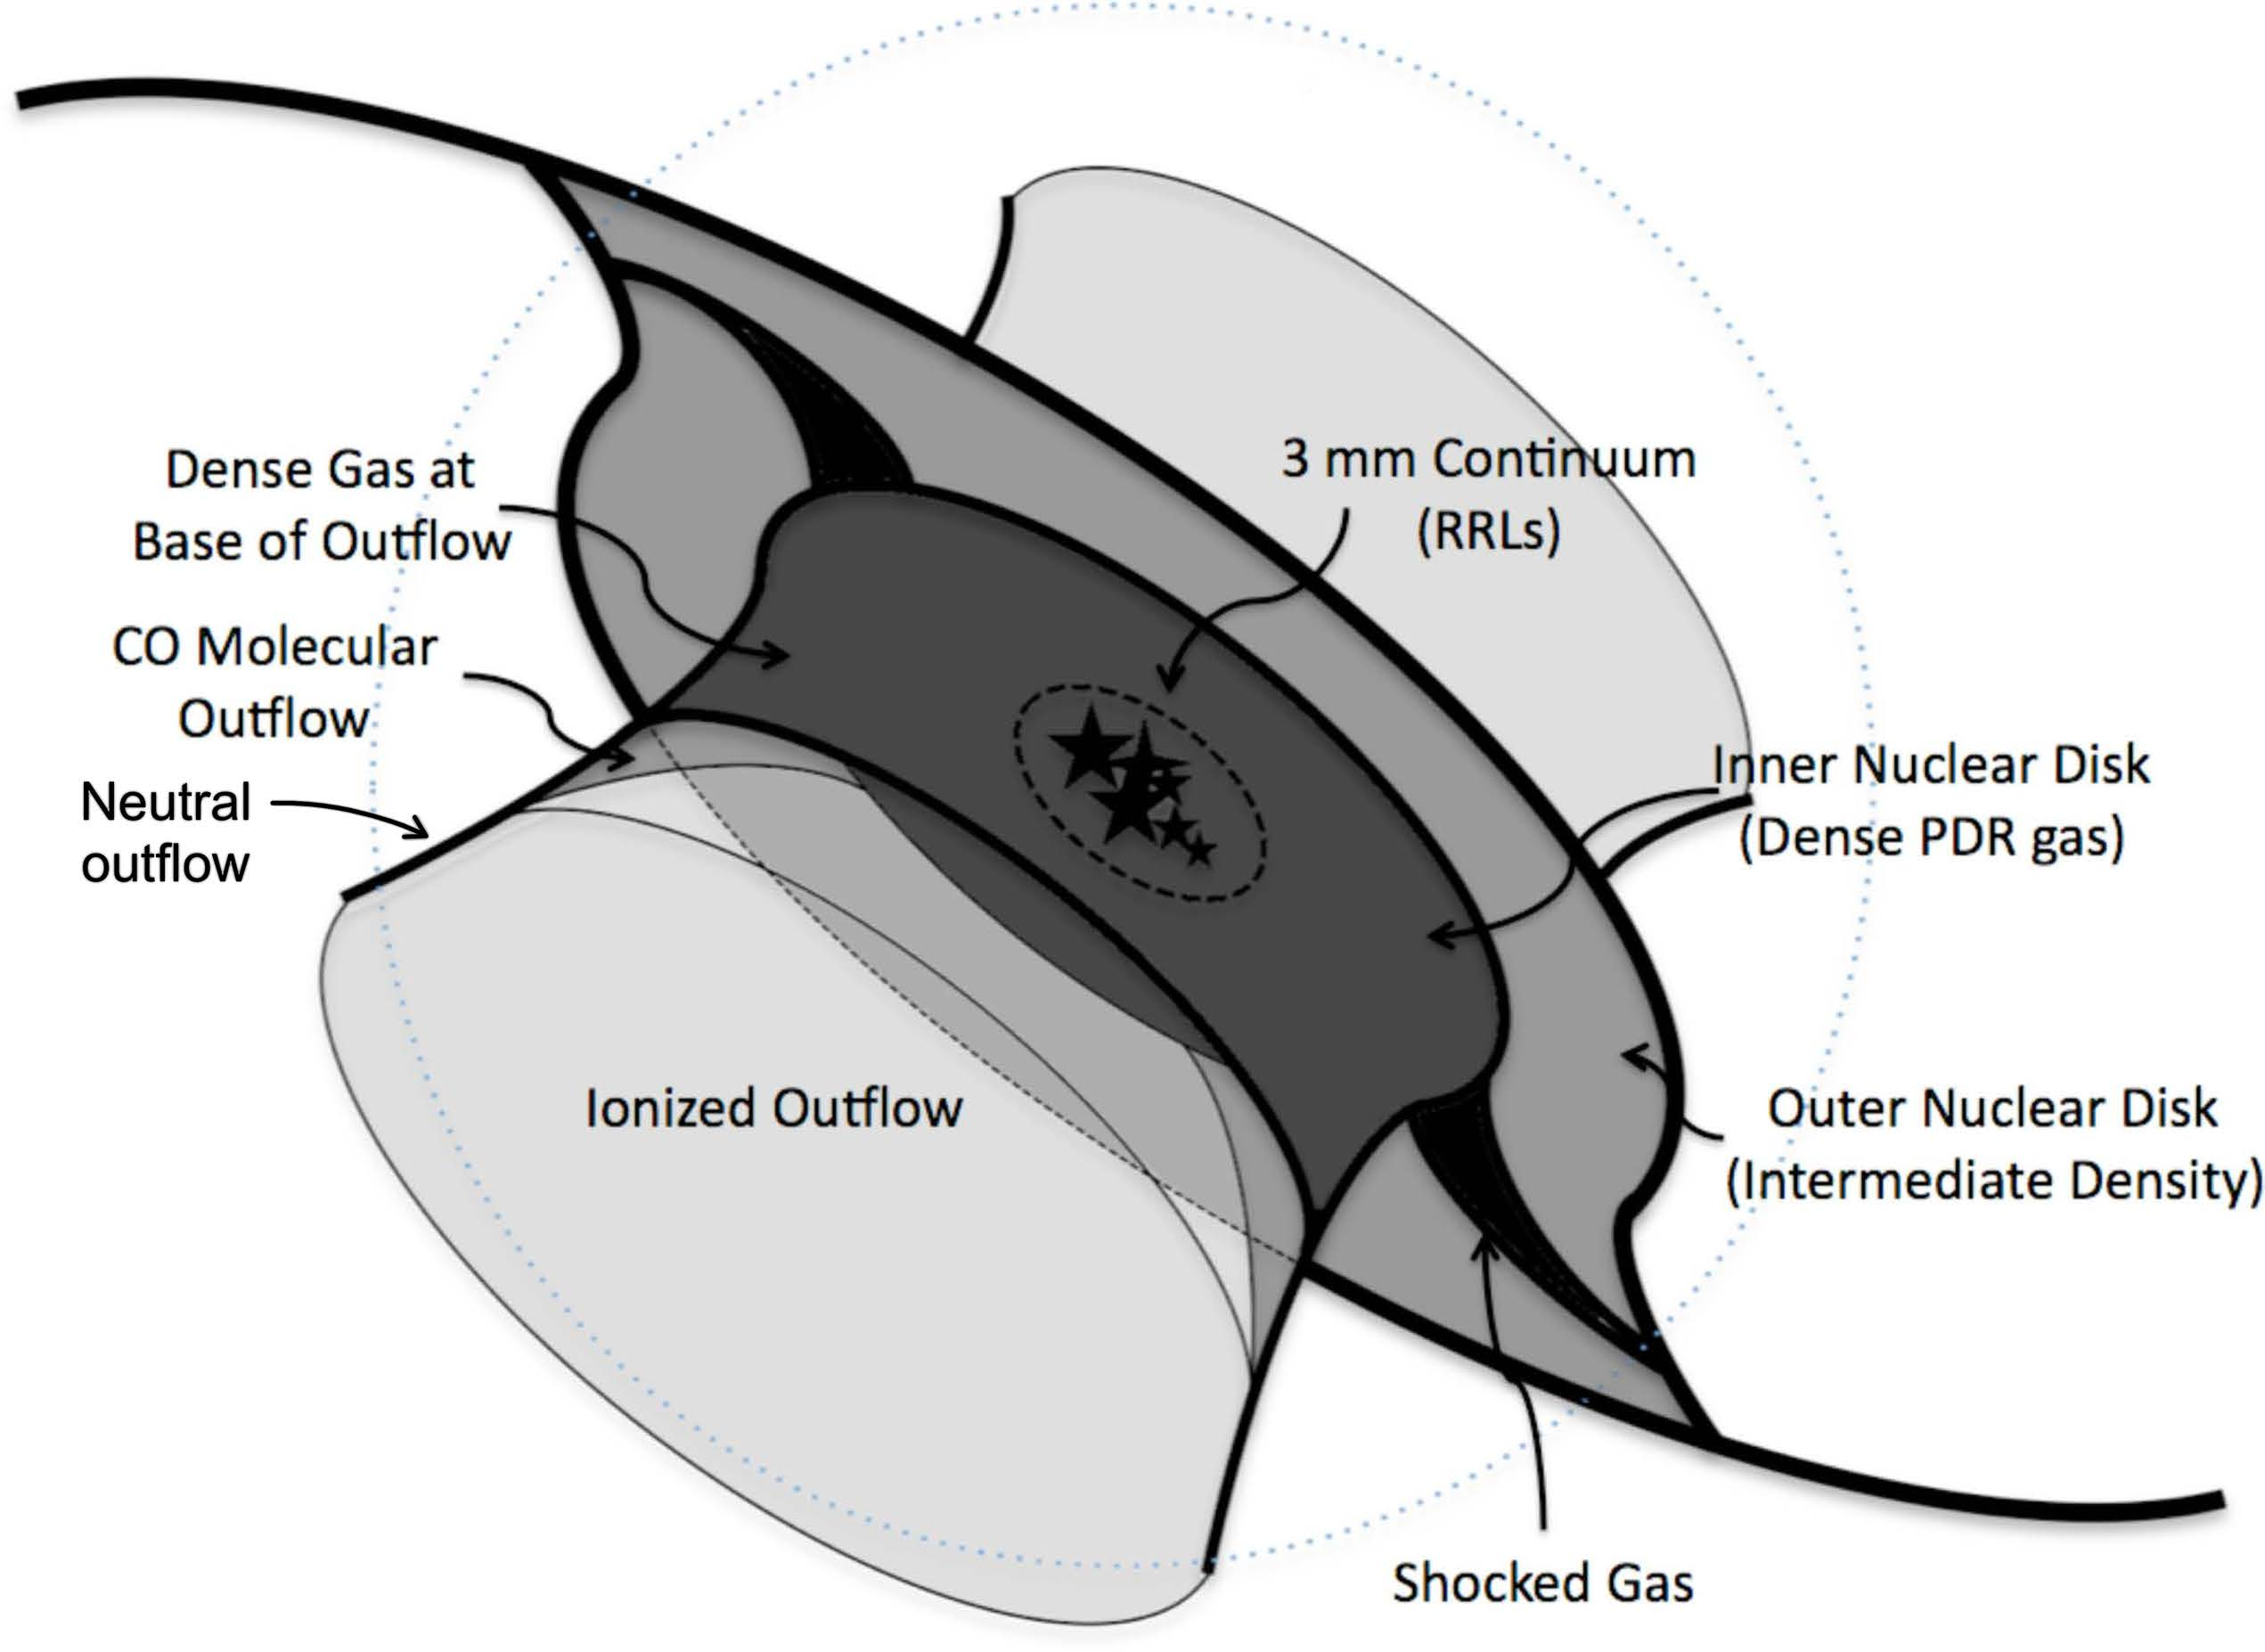
\includegraphics[width=0.7\linewidth]{images/chapters/introduction/sf/outflow_cone.pdf}
	\caption[Schematic of a multi-phase outflow in \ngc253]{Schematic of the multi-phase outflow in \ngc253. The starburst in the center launches a bi-conical stratified outflow. The molecular outflow is thought to be dragged up at the edges of a ionized outflow with a layer of neutral gas in between.
	Figure adapted from \citet{2015ApJ...801...63M}.}
	\label{introduction: figure: star formation: outflow cone}
\end{figure}

Molecular outflows are thus closely intertwined with feedback processes and star formation. The high-resolution structure and kinematic properties of (molecular) outflows have not been studied in detail yet, primarily due to the lack of high resolution and high sensitivity observations. Starburst galaxies are the obvious targets to study star formation-driven outflows due to the high SFR and thus feedback strength in these systems. Consequently, molecular outflows have been studied at tens of parsec scale resolution over the past years in a few nearby starbursts: 
M\,82 \citep{2002ApJ...580L..21W,2015ApJ...814...83L}, NGC\,253 \citep{2013Natur.499..450B,2017ApJ...835..265W,2018ApJ...867..111Z}, NGC\,1808 \citep{2018ApJ...856...97S}, and ESO320-G030 \citep{2016A&A...594A..81P}.


%%%%%%%%%%%%%%%%%%%%%%%%%%%%%%%%%%%%%%%%%%%%%%%%%%%%%%%%%%%%%%%%%%%%%%%%%%%%%%%%%%%%%%%%%%%%%%%%%%%%

\section{Star formation in the cosmological context}
\label{introduction: section: star formation: cosmological context}

\subsection{Cosmic star formation history}

Star formation in galaxies was not steady along the age of the universe but quickly rose in the young universe to then slow down, turn over and decrease \citep[review by][and references therein]{2014ARA&A..52..415M}. The cosmic star formation rate history as shown in Figure~\ref{introduction: figure: star formation: cosmic SFR history} shows this behaviour as a function of redshift and look-back time. At $z\sim2$ when the age of the universe was $\sim 3.5$\,Gyr, the cosmic SFR reached a peak and declined afterwards until today ($z=0$). The shape of the cosmic SFR history is the result of the cosmic expansion starting with the Big Bang and the following coalescence of primordial gas into galaxies that merged into ever larger structures allowing for and triggering star formation. The decline after $z \sim 1.5$ is attributed to a change of accretion mode in galaxies (hot mode vs. cold mode at earlier times) and negative AGN feedback \citep[e.g.][]{2011MNRAS.415.2782V}.

\begin{figure}
	\centering
	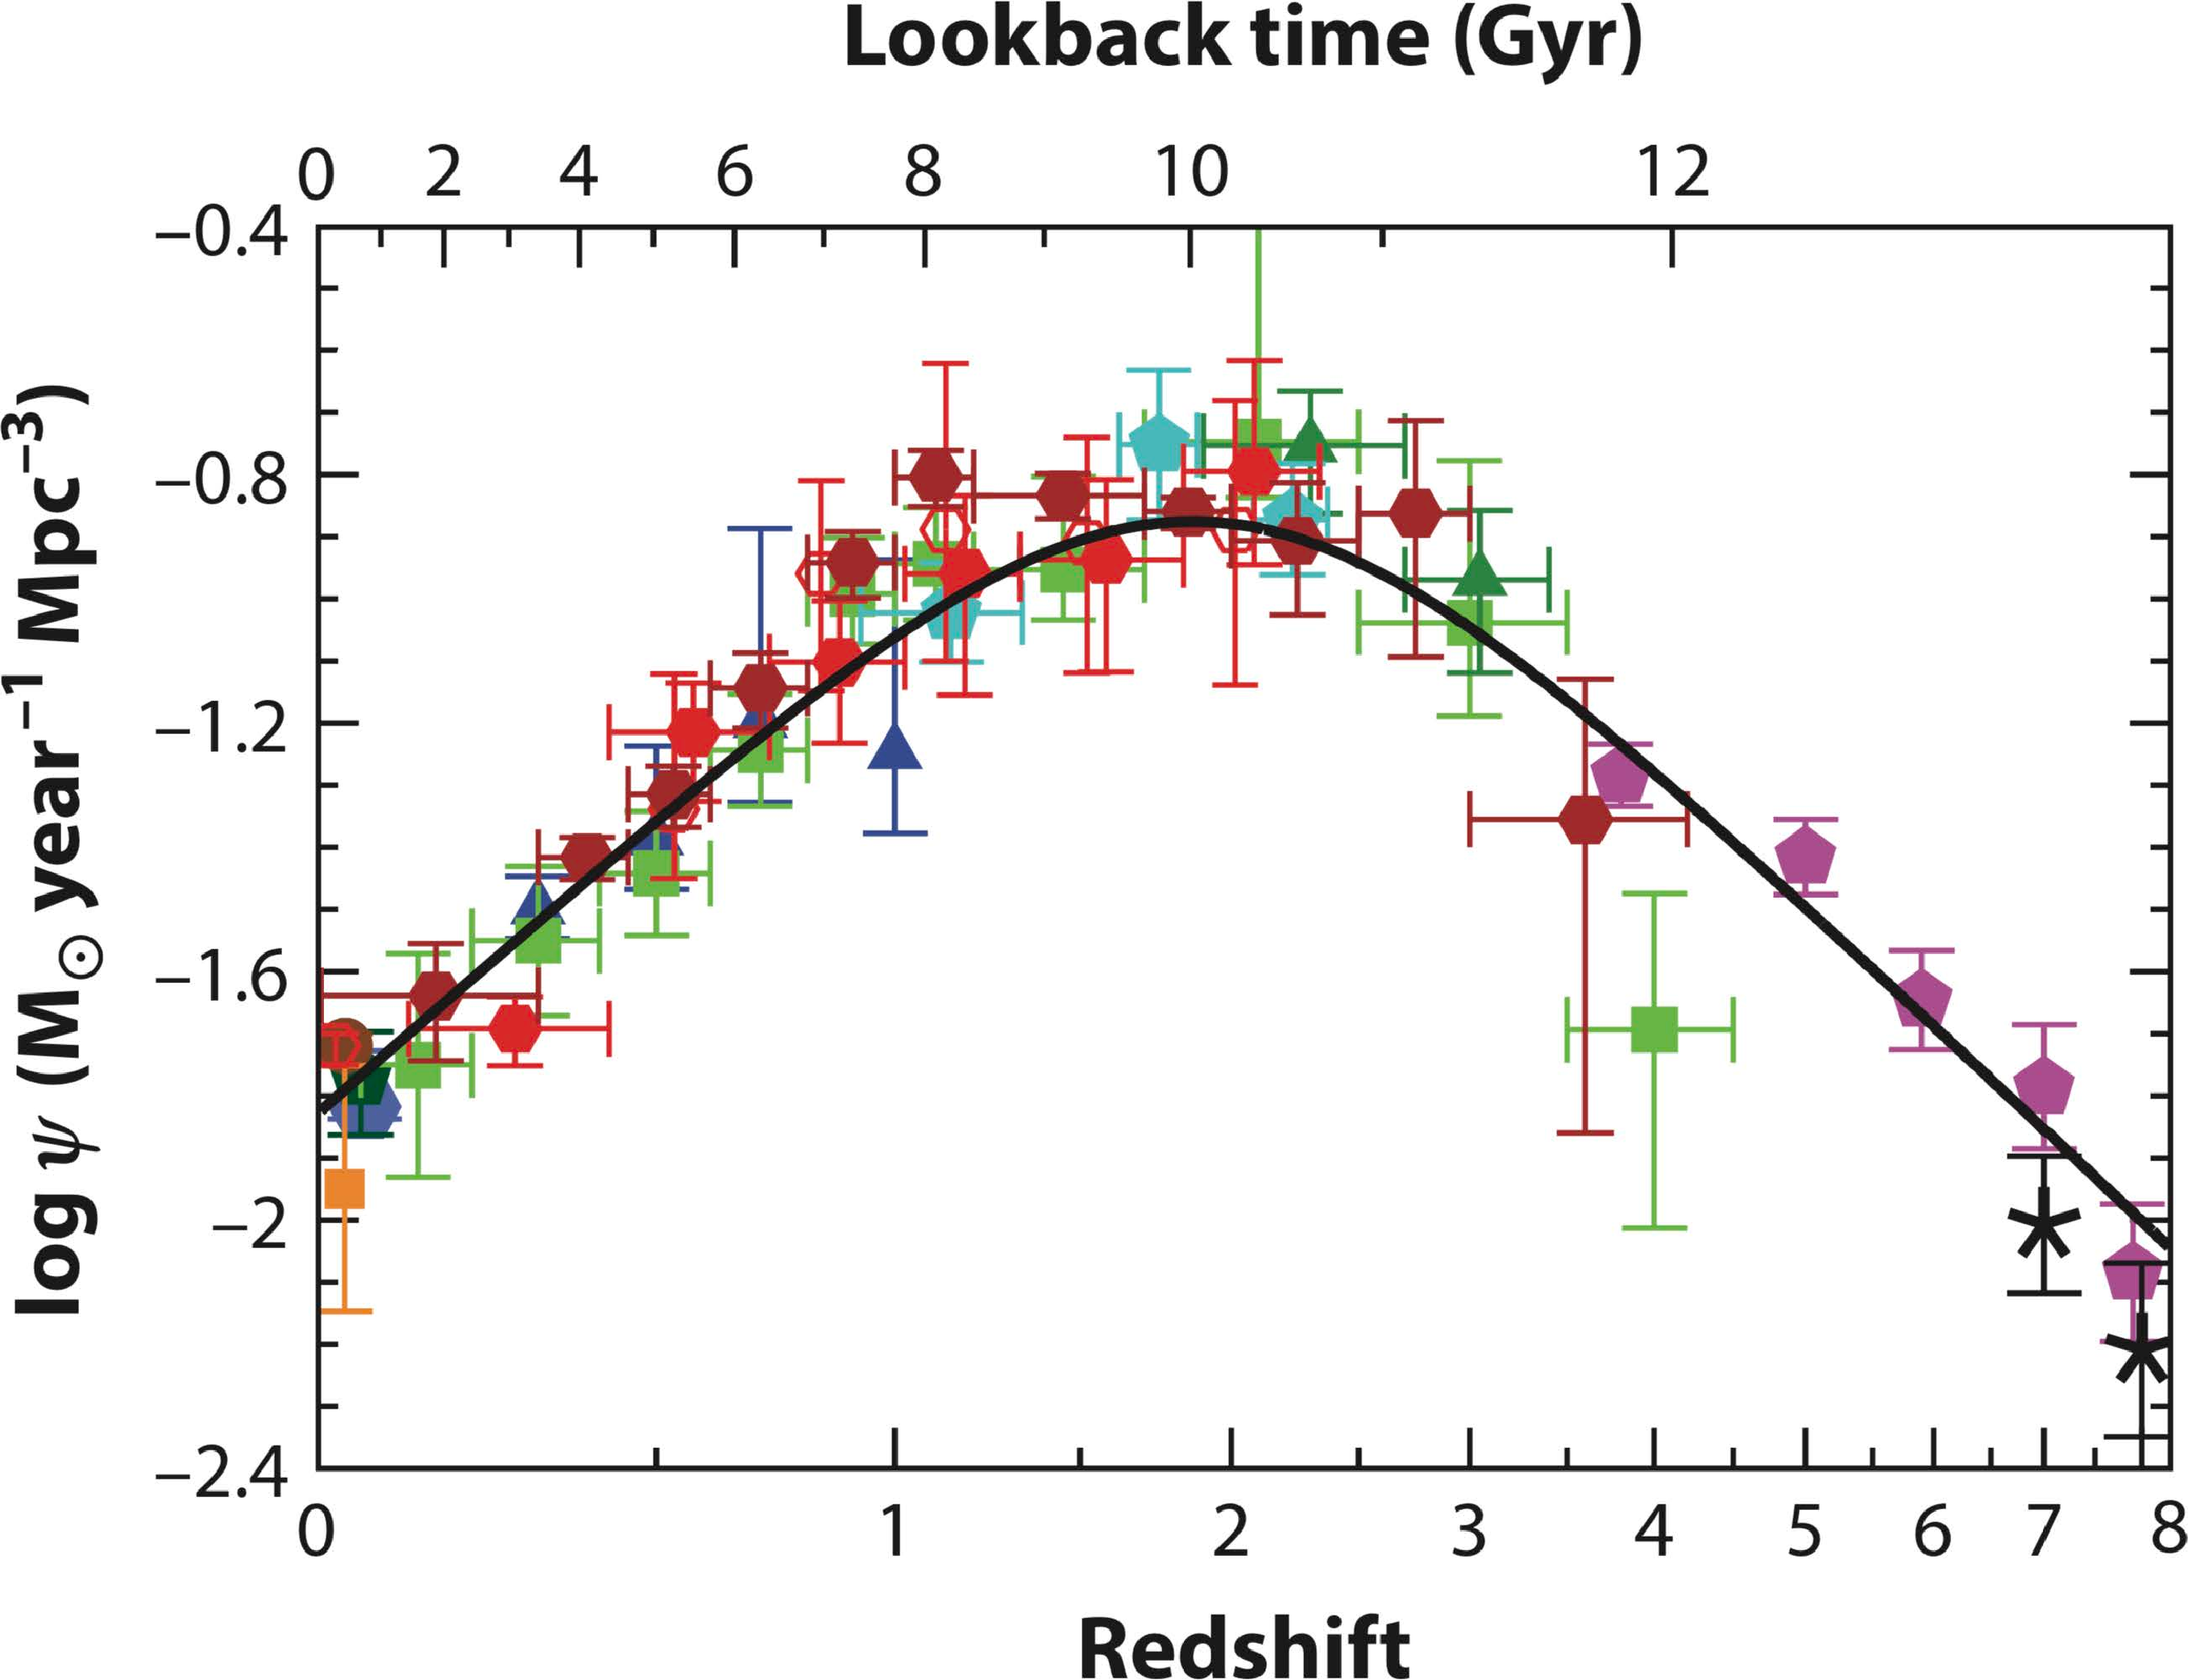
\includegraphics[width=0.6\linewidth]{images/chapters/introduction/sf/csfh.pdf}
	\caption[Cosmic star formation rate history]{Evolution of the cosmic star formation rate density up to redshift $z=8$. In the early universe, star formation quickly became more prevalent and reached a peak at $z\sim2$. At later times, the star formation died down to today's value of $\sim 1$\,\Msunyr per $4^3 = 64$\,Mpc$^3$. At the peak at $z\sim2$, the same volume of the universe had a ten times higher average $SFR \sim 10$\,\Msunyr. Figure adapted from \citet{2014ARA&A..52..415M}.}
	\label{introduction: figure: star formation: cosmic SFR history}
\end{figure}


\subsection{Main sequence evolution}

\begin{figure}
	\centering
	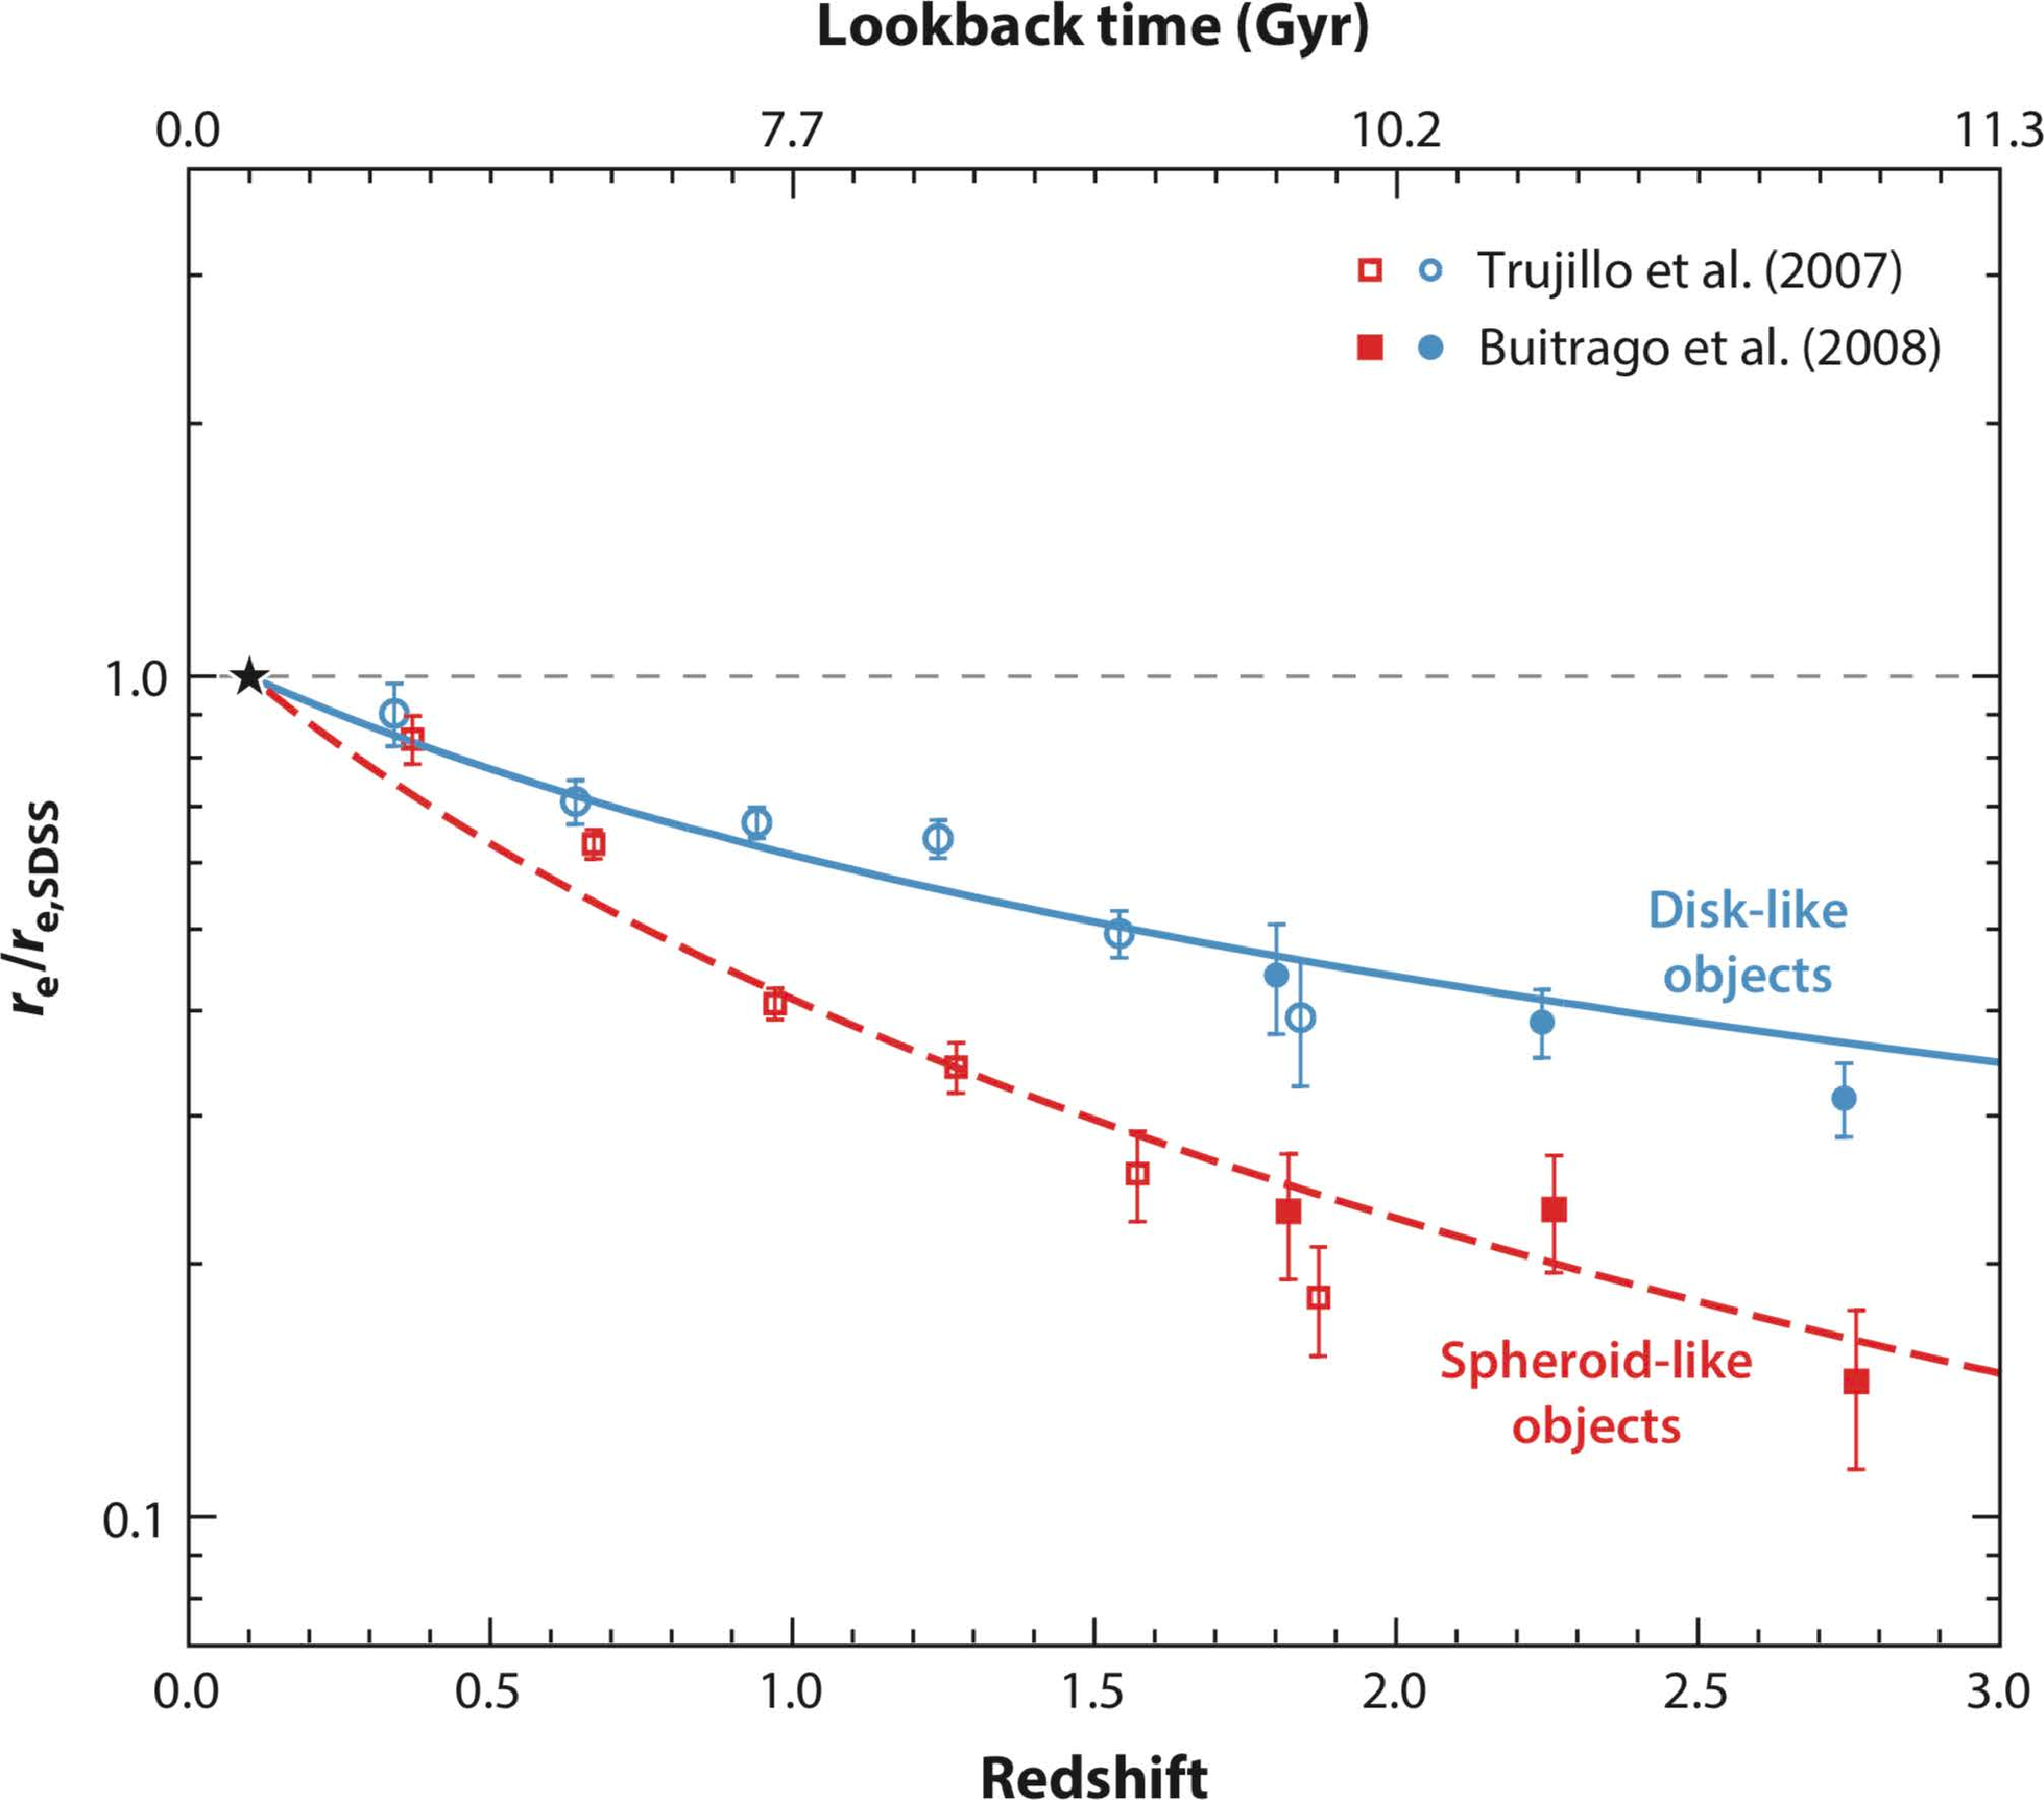
\includegraphics[width=0.6\linewidth]{images/chapters/introduction/sf/size_evolution.pdf}
	\caption[Redshift dependence of galaxy sizes]{Relative average sizes (effective radius $r_\mathrm{e}$) of massive galaxies ($M_* \GTR 10^{11}$\,\Msun) measured by the POWIR and GOODS NICMOS surveys \citep{2007MNRAS.382..109T,2008ApJ...687L..61B}. The reference sizes $r_\mathrm{e,SDSS}$ are derived from $z\sim0$ SDSS galaxies \citep{2003MNRAS.343..978S}. Figure taken from \citet{2014ARA&A..52..291C}.}
	\label{introduction: figure: star formation: galaxy size evolution}
\end{figure}

\begin{figure}
	\centering
	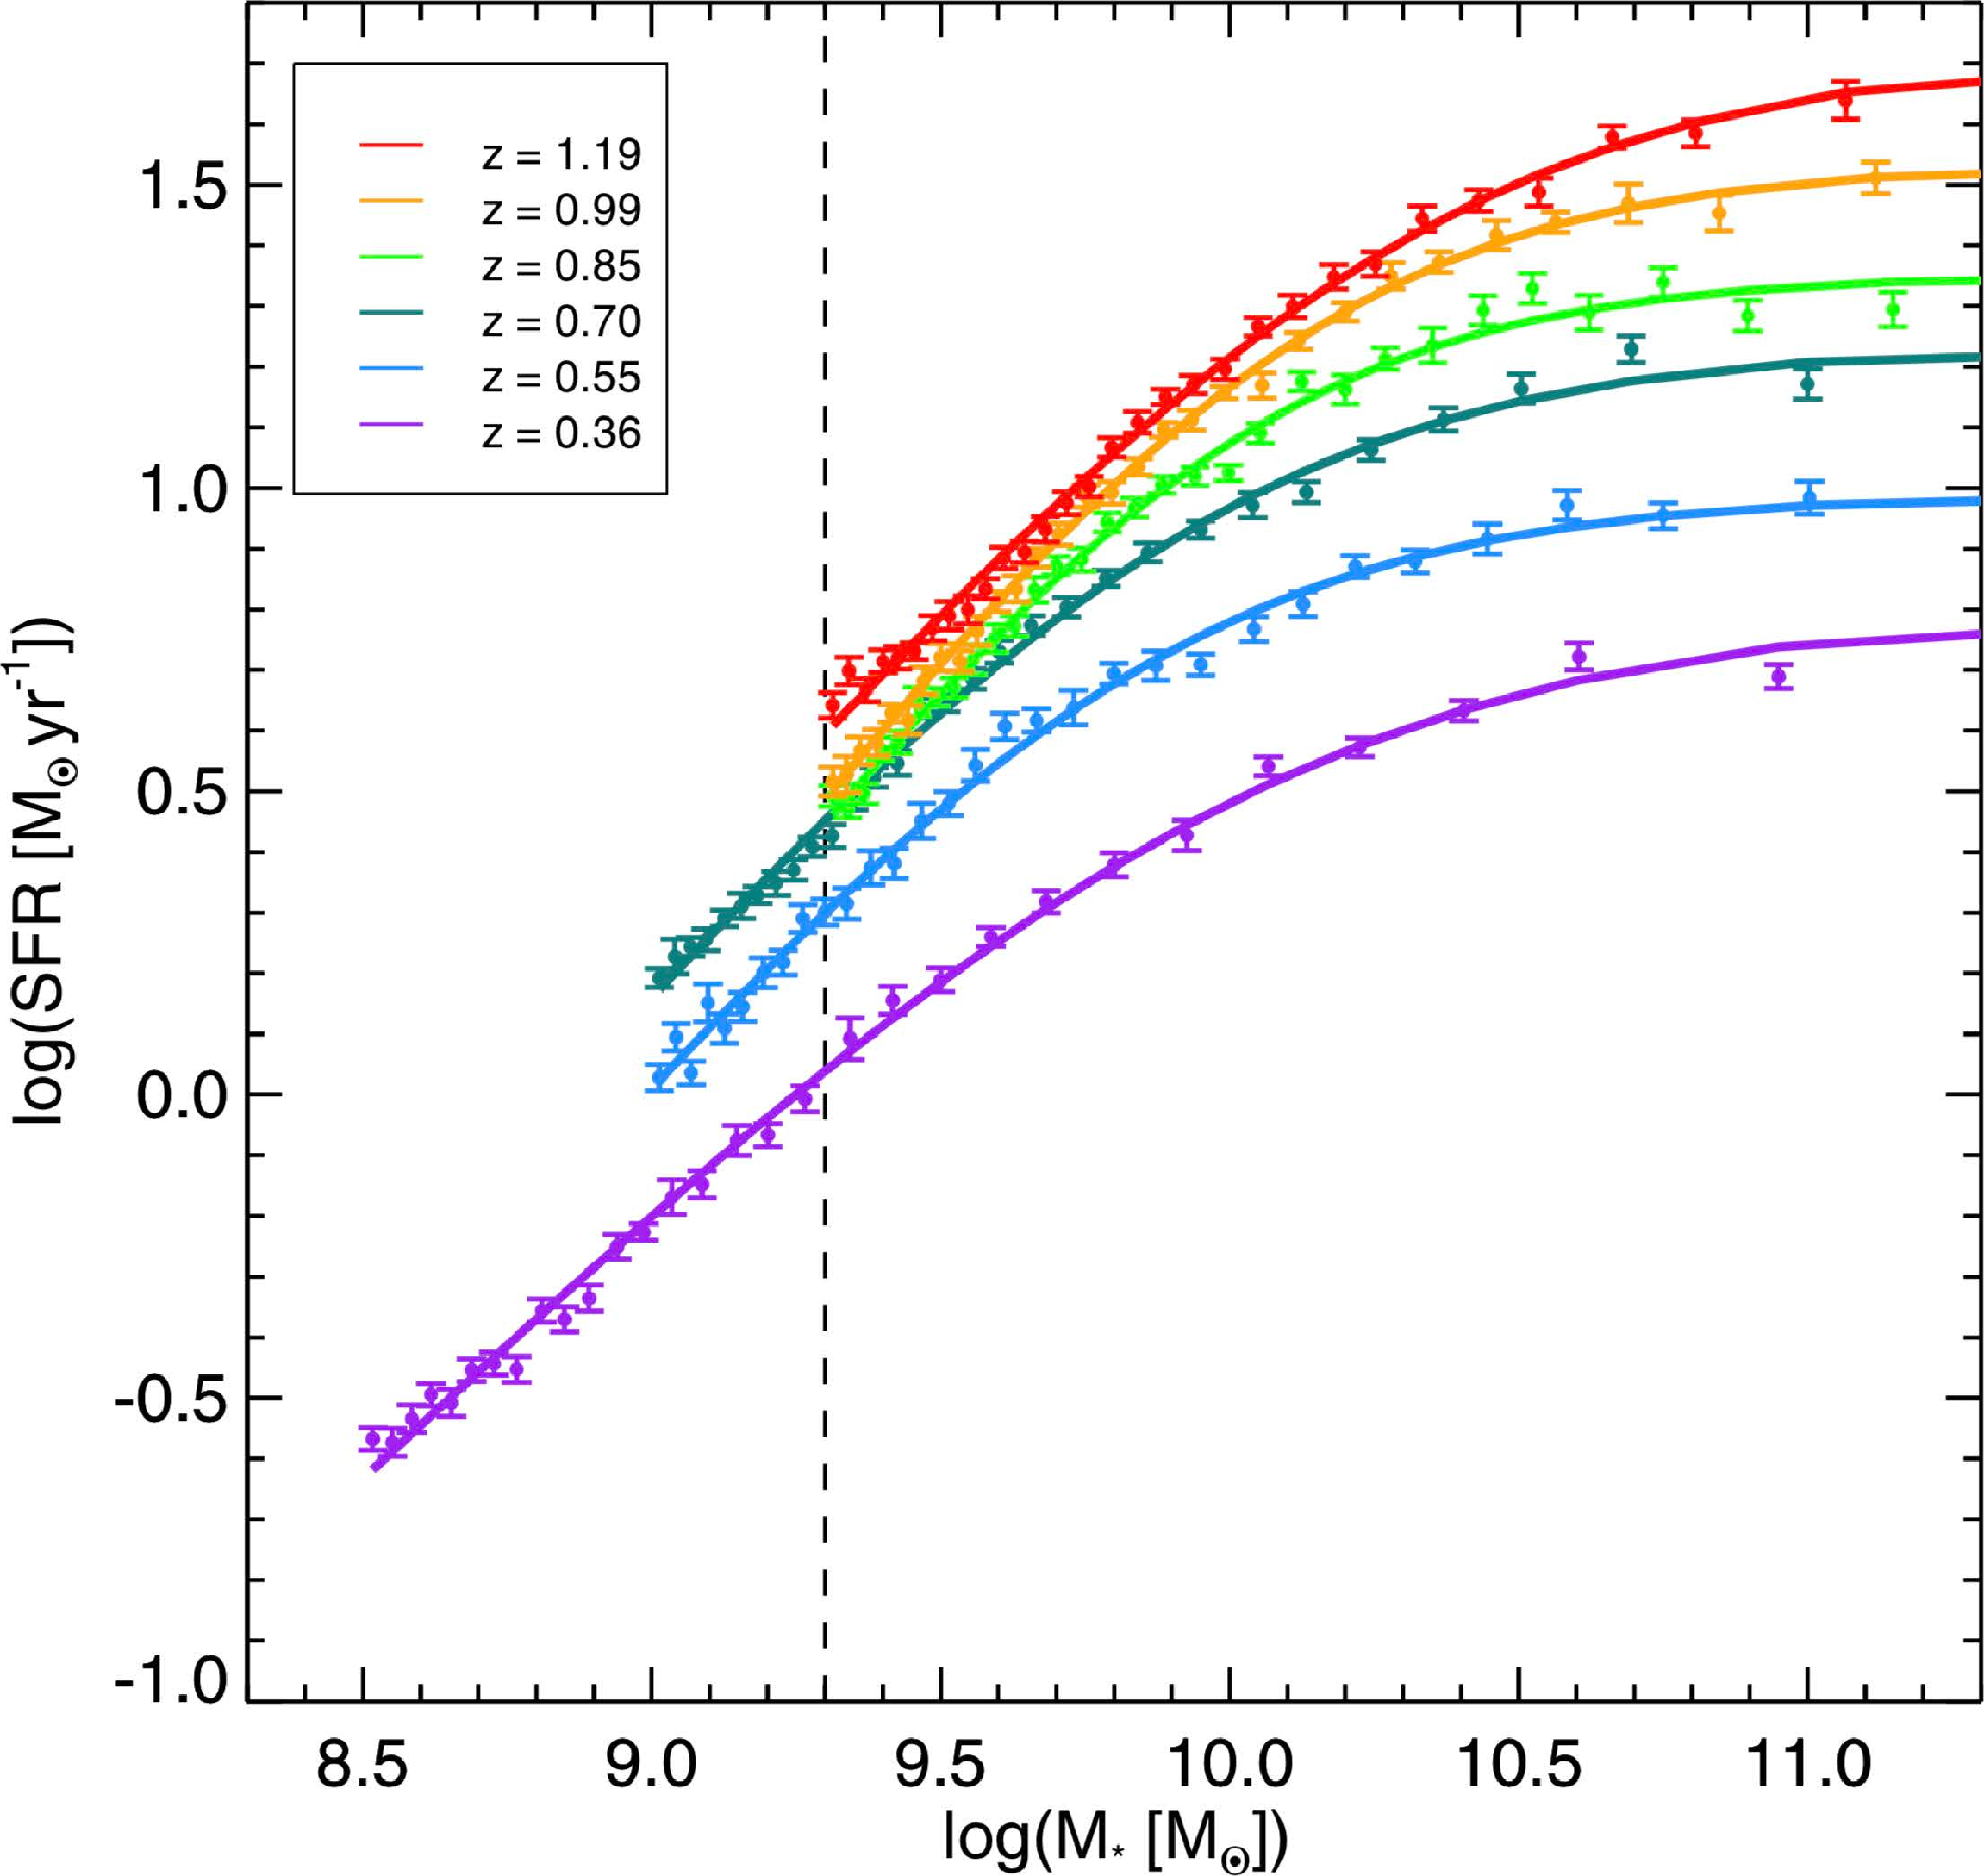
\includegraphics[width=0.6\linewidth]{images/chapters/introduction/sf/ms_shift.pdf}
	\caption[Redshift dependence of the main sequence]{The main sequence of star forming galaxies shifts to higher star formation rate at higher redshift shown here for the range $z =0.36 - 1.19$. In the stellar mass vs. star formation rate plane, a main sequence starforming galaxy at $z \sim 1-2$ would be considered a starburst at $z \sim 0$. Figure taken from \citet{2015ApJ...801...80L}.}
	\label{introduction: figure: star formation: MS shift}
\end{figure}

Similar to the higher SFR density on cosmic scales, the SFR of a typical star forming galaxy also evolves with redshift and is much higher at high-$z$ \citep[e.g.][]{2012ApJ...754L..29W,2014ApJ...795..104W}. Since galaxies grow over time by accretion of gas and galaxy mergers, high-$z$ galaxies are smaller than today's galaxies (Figure~\ref{introduction: figure: star formation: galaxy size evolution}). In combination, a typical high-$z$ star forming galaxy has a greatly enhanced star formation rate surface density $\Sigma_\mathrm{SFR}$ at higher global SFR. The MS (Section~\ref{introduction: section: star formation: main sequence}) thus shifts towards higher SFR with redshift as is shown in Figure~\ref{introduction: figure: star formation: MS shift}. Currently, it is still debated if the shape of the MS also changes with redshift or only shifts up \citep[e.g.][]{2019MNRAS.490.5285P}.

The parameter space above the MS occupied by local ($z \sim 0$) starbursts corresponds to the location of the MS at higher redshift. The correspondence to a particular redshift ($z = 0.5,1,2,...$), of course, depends on the MS offset of the respective starburst. Hence, local starbursts are expected to be analogs or at least proxies to typical star forming galaxies around the peak of the cosmic SFR.


\subsection{Stellar clusters}

As mentioned before in Section~\ref{introduction: section: star formation: SSCs}, SSCs are potential siblings of old globular clusters. To better understand the formation and evolution of globular clusters from local analogs, it must be checked if those local analogs evolve in similar environments and show comparable properties. Observations show that the fraction of stars formed in clusters scales with SFR surface density \citep{2012MNRAS.426.3008K,2016ApJ...827...33J,2018ApJ...864L..17G} and local starbursts show similar $\Sigma_\mathrm{SFR}$ as high-$z$ MS star forming galaxies as explained above. It should therefore be possible to learn more about the formation of the oldest stellar systems by observing SSCs in the nearby universe. Although the general conditions are similar, not much is yet known about the ISM conditions on cluster scales outside the local group. ALMA now offers the resolution and sensitivity to resolve SSCs in e.g. \ngc253 and characterize the physical and chemical properties of the ISM (Chapter~\ref{chapter: SSCs}).


\subsection{The need for local analogs to high-$z$ phenomena}

To resolve the relevant size scales for star formation, ideally pc-scale resolution is required or at least a few tens of pc to resolve GMCs. Achieving such resolutions will be impossible for galaxies at the peak of the cosmic SF history in the short and middle term future. The latest generation of telescopes only achieve resolutions of several hundred pc at $z\GTR1$ --- not nearly enough to resolve SF.
Starbursts as nearby analogs are therefore the most promising and practically the only way to understand how the SF process worked during the most active phase of SF in the universe.

With extremely capable instruments such as ALMA or NOEMA, it is now the time to study the resolved ISM in nearby starbursts to solve how the high-activity mode of SF works and how it affects its host galaxy.


%%%%%%%%%%%%%%%%%%%%%%%%%%%%%%%%%%%%%%%%%%%%%%%%%%%%%%%%%%%%%%%%%%%%%%%%%%%%%%%%%%%%%%%%%%%%%%%%%%%%
%%%%%%%%%%%%%%%%%%%%%%%%%%%%%%%%%%%%%%%%%%%%%%%%%%%%%%%%%%%%%%%%%%%%%%%%%%%%%%%%%%%%%%%%%%%%%%%%%%%%

\chapter{\ngc253}
\chaptermark{\ngc253}
\label{introduction: chapter: NGC253}

%%%%%%%%%%%%%%%%%%%%%%%%%%%%%%%%%%%%%%%%%%%%%%%%%%%%%%%%%%%%%%%%%%%%%%%%%%%%%%%%%%%%%%%%%%%%%%%%%%%%

\vspace{-0.5cm}
\begin{figure*}[h]
	\centering
	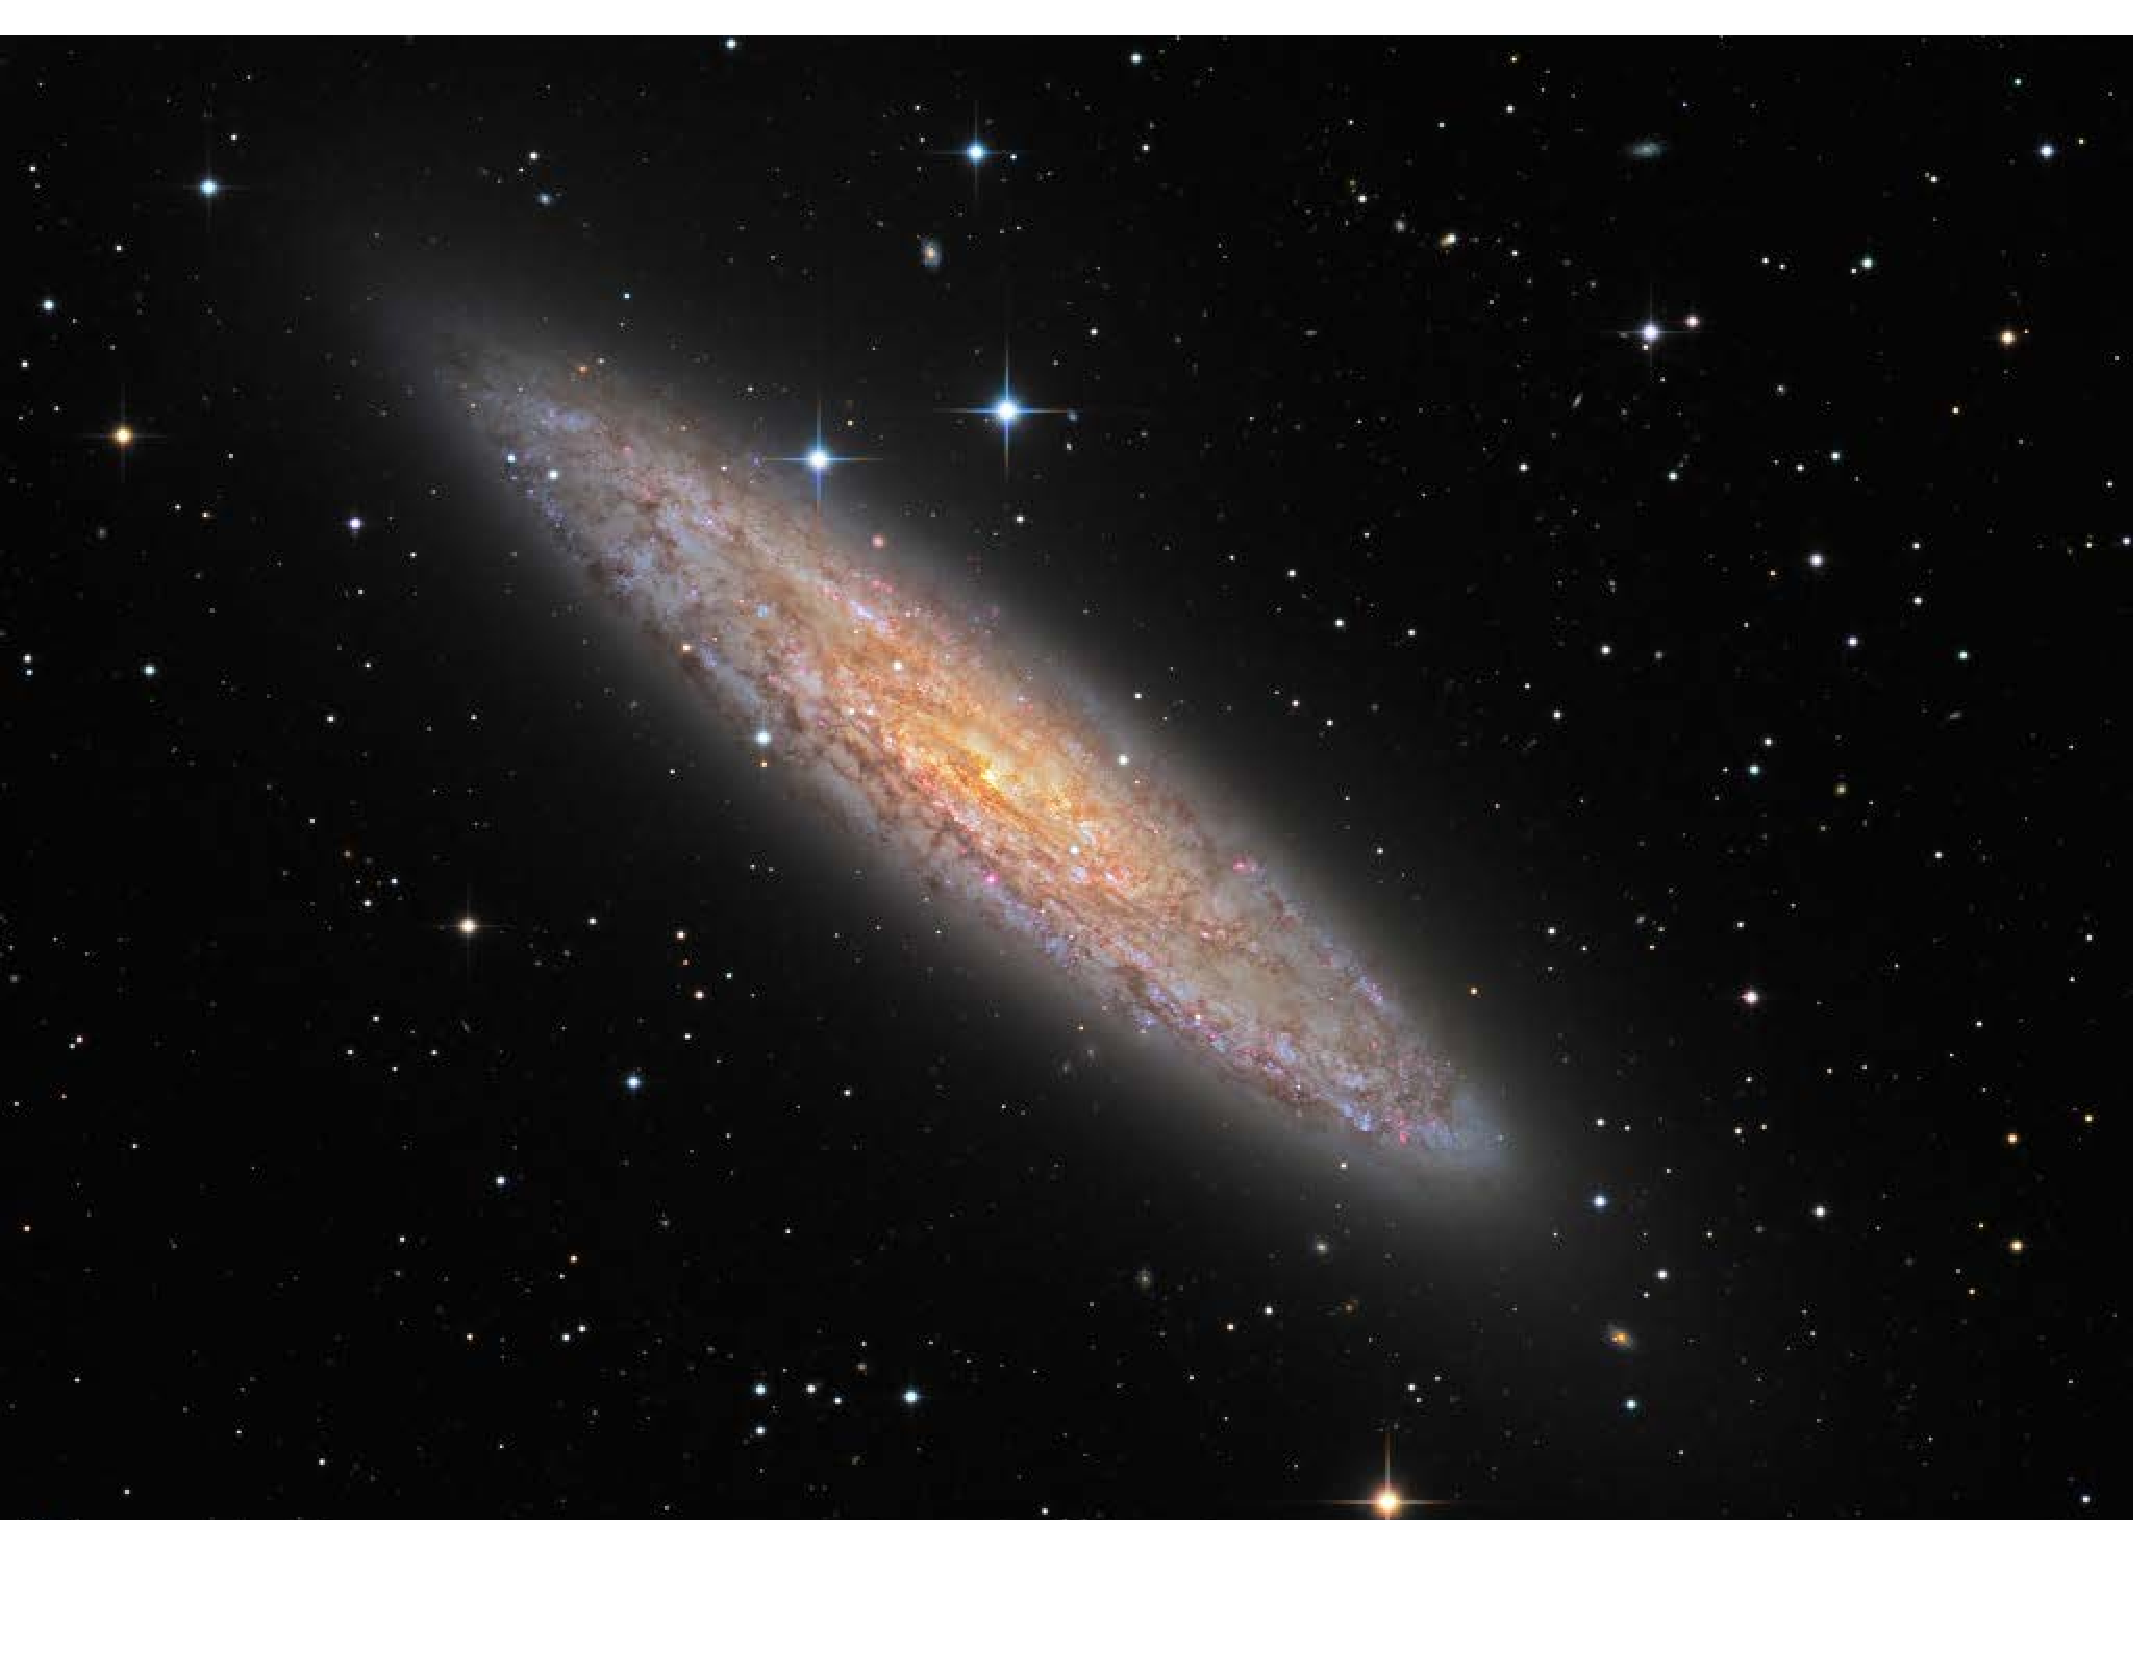
\includegraphics[width=\linewidth]{images/chapters/introduction/ngc253/NGC253_Apod.pdf}
	\caption[Optical image of NGC253]{Optical image of \ngc253. Due to its brightness ($V \sim 7.3$\,mag) and size on the sky ($\sim 30\arcmin$), \ngc253 is a popular target for amateur astronomers who achieve impressive results with extremely long exposure times, 20\,h in this case. Image from \href{https://apod.nasa.gov/apod/ap161103.html}{APOD}, credit: D. Hager, E. Benson}
	\label{introduction: figure: NGC253: optical}
\end{figure*}

\ngc253 is the brightest ($V=7.3$\,mag) galaxy in the Sculptor group, one of the nearest galaxy groups to the local group \citep{2005AJ....129..178K}.
It is also referred to as the Sculptor galaxy or the Silver Coin Galaxy and classified as a barred spiral galaxy (Hubble type SBc).
The stellar mass $M_\ast \sim 4.4 \times 10^{10}$\,\Msun \citep{2011ApJ...736...24B} and total gas mass $M_\mathrm{gas} > 1.3 \times 10^9$\,\Msun \citep{2000PASJ...52..785S}\footnote{Their observations only covered the inner $R<4$\,kpc but not the whole galactic disk.} make \ngc253 a typical L$^\ast$ galaxy, similar to the Milky Way.
Our view on \ngc253 is close to edge-on (inclination $i\sim78^\circ$) and from below the galactic disk.

Due to its proximity, \ngc253 (Figure~\ref{introduction: figure: NGC253: optical}) is an ideal target for high-resolution studies of the physics and chemistry of the star-forming molecular gas and stellar feedback in starbursts.
At a distance of 3.5\,Mpc \citep{Rekola:2005ha}, \ngc253 is one of the nearest starburst systems and considered one of the prototypical starburst galaxies. The star formation rate surface density is $\Sigma_{SFR} \sim 10^2$\,\Msun\,yr$^{-1}$\,kpc$^{-2}$ in the nuclear region which causes the molecular gas depletion time $\tau^\mathrm{mol}_\mathrm{dep}$ to be $\sim 5-25$ times lower than what is found in local disks \citep{Leroy:2015ds}. 
A galactic wind emerges from the central $\sim 200$\,pc of \ngc253 (Figure~\ref{introduction: figure: NGC253: Strickland}) that has been characterized in H$\alpha$, X-ray, as well as neutral and molecular gas emission \citep[e.g.][]{Sharp:2010jl,Turner:1985iy,Sturm:2011jb,Strickland:2000wd,Strickland:2002kp, Westmoquette:2011bp,2000ApJS..129..493H,2013Natur.499..450B,2017ApJ...835..265W}.
The outflow is thought to be stratified with an inner ionized cone and surrounding shells of neutral and molecular gas \citep[as shown in Figure~\ref{introduction: figure: star formation: outflow cone}]{2015ApJ...801...63M}.

\begin{figure*}
	\centering
	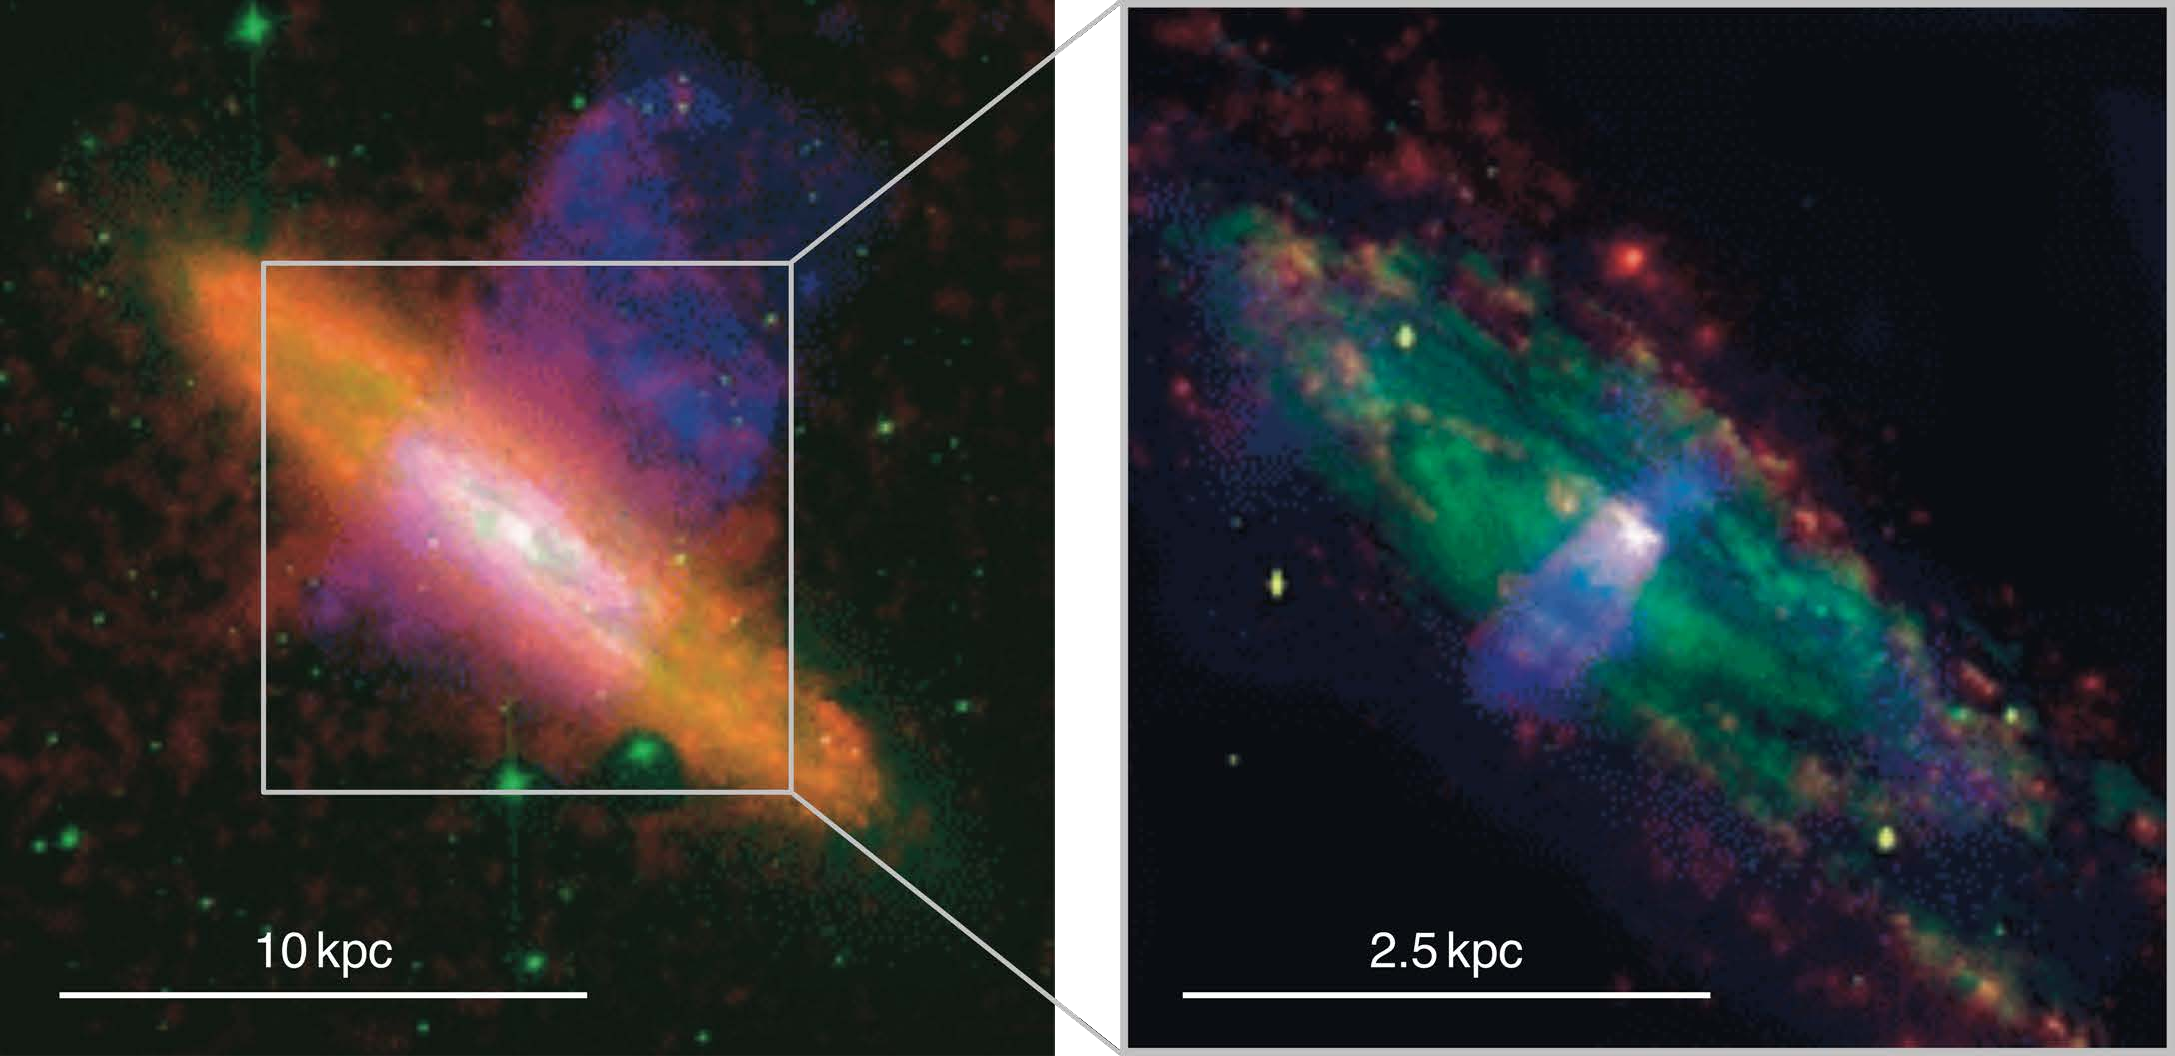
\includegraphics[width=\linewidth]{images/chapters/introduction/ngc253/Strickland+04_combined.pdf}
	\caption[Ionized outflow in \ngc253]{Three color composite image of \ngc253 showing \Halpha (red), optical R band (green) and soft X-ray ($0.3-2.0$\,keV, blue). Figure adopted from \citet{2004ApJ...606..829S}.}
	\label{introduction: figure: NGC253: Strickland}
\end{figure*}

Studies of the molecular gas phase in \ngc253 showed that its central starburst is fueled by gas accretion along the bar \citep{2004ApJ...611..835P}. The molecular ISM in the nuclear region is structured in several clumps that show high temperatures of $\GTRSIM 50$\,K \citep{2004ApJ...611..835P,Sakamoto:2011et,2019ApJ...871..170M}. 

From earlier low resolution observations \citep[$\GTR 20$\,pc, e.g.][]{2006ApJ...636..685S,Sakamoto:2011et} to recent observations at high resolution ($8\,\mathrm{pc}\times5$\,pc in \citealt{2017ApJ...849...81A} and 2\,pc in \citealt{2018ApJ...869..126L}) the number of molecular clumps associated with the starburst increased from $\sim5$ to 14. These studies find the clumps to be massive ($M_\mathrm{mol} \sim 4-10 \times 10^4$\,\Msun), compact ($\LESS 10$\,pc), chemically rich (up to $\GTR 19$ molecules detected in the 0.8\,mm band) and hot (up to 90\,K). 
These massive and dense clumps provide an ideal environment for SSC formation and each clump likely hosts an embedded massive (proto-)SSC \citep{2018ApJ...869..126L}.
It has been known for a while now that \ngc253 hosts at least a single SSC. \citet{Watson:1996dn} and \citet{Kornei:2009ee} detected a young, deeply embedded SSC in HST imaging of the nuclear region. Hints of further SSCs were discovered in radio observations \citep{1997ApJ...488..621U} but do not show obvious counterparts in optical or near-IR imaging \citep{2017ApJ...835..265W}. 
The 14 (proto-)SSCs characterized by \citet{2018ApJ...869..126L} are still deeply embedded in their natal gas and dust clouds. At least some of the SSCs are very young \citep[$\LESS 1$\,Myr][]{2020MNRAS.491.4573R}, with many showing roughly equal, but still uncertain, masses of young stars and gas \citep{2018ApJ...869..126L}.

Further structures in the molecular gas are shells and bubbles blown by stellar feedback. \citet{2006ApJ...636..685S} found two 100\,pc diameter superbubbles. \citet{2013Natur.499..450B} report molecular streamers\footnote{The term {\em streamer} here denotes structures with a high aspect ratio that are typically oriented roughly perpendicular to the disk and often show a velocity gradient.} originating from these shells with a lower limit to the outflow rate of $\dot{M} \sim 3-9$\,M$_\odot$\,yr$^{-1}$, about three times the star formation rate. This estimate was revisited by \citet{2018ApJ...867..111Z}, based on observations that show that the CO emission associated with the most prominent streamer is optically thick, increasing it to $25-50$\,\Msunyr. The impact of the outflows on the amount of mass lost from the molecular gas reservoir, and thus the lifetime of the starburst, is significant. 


\cleardoublepage%%%%%%%%%%%%%%%%%%%%%%%%%%%%%%%%%%%%%%%%%%%%%%%%%%%%%%%%%%%%%%%%%%%%%%%%%%%%%%%%%%%%%%%%%%%%%%%%%%%%

% \ctparttext{This part contains the three published papers and some additional unpublished work as the main part of the thesis.}
\part*{The molecular ISM in and around the starburst in NGC253}
\label{part: papers}

%%%%%%%%%%%%%%%%%%%%%%%%%%%%%%%%%%%%%%%%%%%%%%%%%%%%%%%%%%%%%%%%%%%%%%%%%%%%%%%%%%%%%%%%%%%%%%%%%%%%

%%%%%%%%%%%%%%%%%%%%%%%%%%%%%%%%%%%%%%%%%%%%%%%%%%%%%%%%%%%%%%%%%%%%%%%%%%%%%%%%%%%%%%%%%%%%%%%%%%%%

\chapter{The Molecular Outflow in \ngc253 at a Resolution of Two Parsecs}
\chaptermark{the molecular outflow in \ngc253}
\label{chapter: outflow}

%%%%%%%%%%%%%%%%%%%%%%%%%%%%%%%%%%%%%%%%%%%%%%%%%%%%%%%%%%%%%%%%%%%%%%%%%%%%%%%%%%%%%%%%%%%%%%%%%%%%

\begin{papernote}
This chapter including appendix~\ref{appendix: outflow} comprises the peer-reviewed article of the same title \citep{2019ApJ...881...43K}. The published paper has been reformatted to match the style of this thesis.
\end{papernote}


\begin{paperabstract}
We present 0.15\arcsec ($\sim2.5$\,pc) resolution ALMA \co32 observations of the starbursting center in \ngc253. Together with archival ALMA \co10 and \co21 data we decompose the emission into a disk and non--disk component. 
We find $\sim7-16\%$ of the CO luminosity to be associated with the non-disk component ($1.2-4.2 \times 10^7$\,\Kkmspc). The total molecular gas mass in the center of \ngc253 is $\sim3.6\times10^8$\,M$_\odot$ with $\sim0.5\times10^8$\,M$_\odot$ ($\sim15\%$) in the non-disk component. These measurements are consistent across independent mass estimates through three CO transitions. 
The high-resolution \co32 observations allow us to identify the molecular outflow within the non-disk gas. Using a starburst conversion factor, we estimate the deprojected molecular mass outflow rate, kinetic energy and momentum in the starburst of \ngc253. The deprojected molecular mass outflow rate is in the range $\sim 14-39$\,\Msunyr with an uncertainty of 0.4\,dex. The large spread arises due to different interpretations of the kinematics of the observed gas while the errors are due to unknown geometry. The majority of this outflow rate is contributed by distinct outflows perpendicular to the disk, with a significant contribution by diffuse molecular gas. This results in a mass loading factor $\eta = \dot{M}_\mathrm{out} / \dot{M}_\mathrm{SFR}$ in the range $\eta\sim8-20$ for gas ejected out to $\sim300$\,pc. 
We find the kinetic energy of the outflow to be $\sim2.5-4.5\times10^{54}$\,erg and $\sim0.8$\,dex typical error which is $\sim0.1$\% of the total or $\sim8$\% of the kinetic energy supplied by the starburst. The outflow momentum is $4.8-8.7\times10^8$\,\Msunkms ($\sim0.5$\,dex error) or $\sim2.5-4$\% of the kinetic momentum released into the ISM by feedback. 
The unknown outflow geometry and launching sites are the primary source of uncertainty in this study.
\end{paperabstract}


%%%%%%%%%%%%%%%%%%%%%%%%%%%%%%%%%%%%%%%%%%%%%%%%%%%%%%%%%%%%%%%%%%%%%%%%%%%%%%%%%%%%%%%%%%%%%%%%%%%%
%%%%%%%%%%%%%%%%%%%%%%%%%%%%%%%%%%%%%%%%%%%%%%%%%%%%%%%%%%%%%%%%%%%%%%%%%%%%%%%%%%%%%%%%%%%%%%%%%%%%

\section{Introduction}

Outflows driven by star formation are thought to be a crucial driver of galaxy evolution. Strong stellar feedback caused by high star formation rate densities can launch outflows of ionized, neutral and molecular gas that potentially can escape the main body of a galaxy. Consequently, such outflowing gas removes the potential fuel for future star formation. Therefore, outflows can suppress and quench star formation, as also demonstrated by theoretical predictions and simulations \citep[e.g.][]{1986ApJ...303...39D,2017MNRAS.466.1213K,2018ApJ...857..116M}. Depending on the velocity of the outflow and a galaxy's escape velocity, outflowing gas can be re--accreted at later cosmic times (the so--called `galactic fountain') or leave the system altogether. This process thus has the potential to enrich the galactic disk and circum--galactic medium with heavy metals \citep[e.g.][]{Oppenheimer:2006eq,2010MNRAS.406.2325O,Hopkins:2012ez,Christensen:2018ka}.

Galactic outflows are a multi--phase phenomenon and are observed across the electro--magnetic spectrum from X-ray \citep[e.g.][]{2007ApJ...658..258S}, UV \citep[e.g.][]{2005ApJ...619L..99H}, optical like H$\alpha$ \citep[e.g.][]{2009ApJ...696..192W} to IR \citep[e.g.][]{2009ApJ...700L.149V}, cold dust \citep[e.g.][]{2010A&A...518L..66R}, PAH emission \citep[e.g.][]{2006ApJ...642L.127E}, and sub-millimeter to radio including H\textsc{i} \citep[e.g.][]{2013Natur.499..450B,2015ApJ...814...83L,Lucero:2015if}. Typically, large-scale outflow features at high relative velocity (100s-1000s \kms) are observed in the ionized and neutral gas, whereas molecular outflows often appear as smaller, more compact features \citep{Strickland:2002kp,Westmoquette:2011bp}. The latter are nonetheless important as they dominate the mass budget \citep{2015ApJ...814...83L}. In some galaxies, the gas phases seem to be stratified with an inner ionized outflow cone, a surrounding neutral shell, and molecular gas situated along the outer edge \citep[e.g.][]{2015ApJ...801...63M}. Typically, the outflows originate from an extended region, so the apparent outflow cone has its tip cut-off. 

Molecular outflows are thus closely intertwined with feedback processes and star formation. The high-resolution structure and kinematic properties of (molecular) outflows are not studied in great detail yet, primarily due to the lack of high resolution and sensitivity observations. Starburst galaxies are the obvious target to study star formation-driven outflows due to the high star formation rates (SFR) in these system. Consequently, molecular outflows have been studied over the past years in a few nearby starbursts: M\,82 \citep{2002ApJ...580L..21W,2015ApJ...814...83L}, \ngc253 \citep{2013Natur.499..450B,2017ApJ...835..265W,2018ApJ...867..111Z}, NGC\,1808 \citep{2018ApJ...856...97S}, and ESO320-G030 \citep{2016A&A...594A..81P}.

\ngc253 is one of the nearest starburst systems at a distance of 3.5\,Mpc \citep{Rekola:2005ha}. It is considered one of the prototypical starburst galaxies with a star formation rate surface density of $\Sigma_{SFR} \sim 10^2$\,\Msun\,yr$^{-1}$\,kpc$^{-2}$ in the nuclear region and a molecular depletion time that is $\tau^{mol}_{dep} \sim 5-25$ times lower than what is found in local disks \citep{Leroy:2015ds}. A galactic wind emerges from the central $\sim 200$\,pc of \ngc253 that has been characterized in H$\alpha$, X-ray, as well as neutral and molecular gas emission \citep[e.g.][]{Sharp:2010jl,Turner:1985iy,Sturm:2011jb,Strickland:2000wd,Strickland:2002kp, Westmoquette:2011bp,2000ApJS..129..493H,2013Natur.499..450B,2017ApJ...835..265W}.
Due to the close proximity, starburst and galactic winds can be studied in detail and individual structures can be resolved.

Studies of the molecular gas phase in \ngc253 showed that its central starburst is fueled by gas accretion along the bar \citep{2004ApJ...611..835P}. The molecular ISM in the nuclear region is structured in several clumps that show high temperatures of $\sim 50$\,K \citep{2004ApJ...611..835P,Sakamoto:2011et,2019ApJ...871..170M}. From earlier low resolution observations \citep[$\GTR 20$\,pc, e.g.][]{2006ApJ...636..685S,Sakamoto:2011et} to recent observations at high resolution ($8\,\mathrm{pc}\times5$\,pc in \citealt{2017ApJ...849...81A} and 2\,pc in \citealt{2018ApJ...869..126L}) the number of molecular clumps associated the starburst increased from $\sim5$ to 14. These studies find the clumps to be massive ($4-10 \times 10^4$\,\Msun), compact ($\LESS 10$\,pc), chemically rich (up to $\GTR 19$ molecules detected in the 0.8\,mm band) and hot (up to 90\,K). Each clump likely hosts an embedded massive star cluster \citep{2018ApJ...869..126L}. Further structures in the molecular gas are shells and bubbles blown up by feedback from  the intense star formation process. \citet{2006ApJ...636..685S} found two 100\,pc diameter superbubbles. \citet{2013Natur.499..450B} report molecular streamers\footnote{The term {\em streamer} here denotes structures with a high aspect ratio that are typically oriented roughly perpendicular to the disk and often show a velocity gradient.} originating from these shells with a lower limit to the outflow rate of $3-9$\,M$_\odot$\,yr$^{-1}$, about three times the star formation rate. This estimate was revisited by \citet{2018ApJ...867..111Z}, based on observations that show that the CO emission associated with the most prominent streamer is optically thick, increasing it to $25-50$\,\Msunyr.

As suggested by these studies, the outflow rate in \ngc253 is factors of a few to potentially $\GTR 10$ larger than the star formation rate. Hence, the impact of the outflows on the amount of material lost from the molecular gas reservoir, and thus the lifetime of the starburst, is significant. The availability of new data makes it interesting to revisit the determination of the mass outflow rate in \ngc253, while also removing some limitations of  previous determinations. \citet{2013Natur.499..450B} estimated the outflow rate from a few massive molecular streamers, but did not include potential diffuse outflowing gas. Also, resolution plays an important role in the ability to disentangle outflows from material in the starbursting disk. New ALMA band~7 observations provide excellent spatial resolution and reasonable surface brightness sensitivity. This information enables increasingly accurate determination of the total mass outflow rate, and its impact on the starburst.

In this work, we present ALMA \co32 observations carried out in cycle 3 and 4 that target the molecular gas in the central $\sim 750$\,pc of \ngc253. Together with ancillary band 3 and 6 data from our previous work \citep{2013Natur.499..450B,2015ApJ...801...63M,Leroy:2015ds,2018ApJ...867..111Z}, we have an inventory of three CO lines to study the molecular gas in the starbursting disk and a kinematically different component that includes the outflow. By decomposing the detected emission, we aim to measure the total molecular gas outflow rate in \ngc253 and improve upon previous less systematic results.

Throughout this paper, we adopt a distance of 3.5\,Mpc to \ngc253 \citep{Rekola:2005ha} at which 1\arcsec\ corresponds to 17\,pc. We also define the ``center'' of the nuclear region of \ngc253 to be the kinematic center at $\alpha, \delta = 00^h47^m33.134^s, -25^\circ17^m19.68^s$ as identified in \citet{MullerSanchez:2010dr}.
The paper is structured as follows: In Section~\ref{outflow: section: data reduction}, we describe observational setup and data reduction, and show the results in the form of channel maps, moment maps and position-velocity diagrams. Our approach on separating gas in the star-forming disk from potentially outflowing gas is laid out in Section~\ref{outflow: section: disk separation}. Section~\ref{outflow: section: results separated disk/non-disk} discusses the derived quantities such as CO luminosities, molecular gas masses, outflow rate, kinetic energy and momentum. Our conclusions are summarized in Section~\ref{outflow: section: summary}.


%%%%%%%%%%%%%%%%%%%%%%%%%%%%%%%%%%%%%%%%%%%%%%%%%%%%%%%%%%%%%%%%%%%%%%%%%%%%%%%%%%%%%%%%%%%%%%%%%%%%
%%%%%%%%%%%%%%%%%%%%%%%%%%%%%%%%%%%%%%%%%%%%%%%%%%%%%%%%%%%%%%%%%%%%%%%%%%%%%%%%%%%%%%%%%%%%%%%%%%%%

\section{Data Reduction and Imaging}
\label{outflow: section: data reduction}

\begin{table}
  \centering
  \begin{threeparttable}
    \caption{Details of the datasets used in this analysis.
 	    \label{outflow: table: used datasets}}
%  	\vspace*{10mm}
    \begin{tabular}{lccc}
      \toprule
      & \co10 & \co21 & \co32\\
      \midrule
        ALMA ID				& 2011.1.00172.S		 	 & 2012.1.00108.S			  & 2015.1.00274.S\\
        spatial resolution	& $1.85\arcsec \times 1.32\arcsec$ 	 & $1.70\arcsec \times 1.02\arcsec$	  & $0.17\arcsec \times 0.13\arcsec$\\
        & 31.4\,pc $\times$ 22.4\,pc & 28.8\,pc $\times$ 17.3\,pc & 2.9\,pc $\times$ 2.2\,pc\\
        spectral resolution	& 5.0\,\kms					 & 5.0\,\kms				  & 2.5\,\kms\\
        RMS noise per channel & 1.99\,m\jybeam             & 2.19\,m\jybeam             & 0.81\,m\jybeam\\
        & 75\,mK					 & 29\,mK					  & 0.37\,K\\
      \bottomrule
    \end{tabular}
  \end{threeparttable}
\end{table}


%%%%%%%%%%%%%%%%%%%%%%%%%%%%%%%%%%%%%%%%%%%%%%%%%%%%%%%%%%%%%%%%%%%%%%%%%%%%%%%%%%%%%%%%%%%%%%%%%%%%

\subsection{Data reduction}
\label{outflow: subsection: data reduction}

The data presented in this paper are based on observations in ALMA cycles~2, 3 and 4 in bands~3, 6 and 7 that cover the redshifted emission in \ngc253 of \co10, \co21 and \co32 as well as other molecular lines.
For data reduction and imaging of the band~3 and 6 data see \citet{2013Natur.499..450B}, \citet{Leroy:2015ds}, \citet{2015ApJ...801...63M} and \citet{2018ApJ...867..111Z}. Table~\ref{outflow: table: used datasets} gives an overview of the datasets used in this analysis.

For the band~7 observations, we tuned the lower side band to $342.0-345.8$\,GHz and the upper side band to $353.9-357.7$\,GHz (total bandwidth 7.6\,GHz) with 976.6\,kHz channel width (corresponding to 0.8\,\kms). We targeted the central $\sim 750$\,pc of \ngc253 in a linear four pointing mosaic with two configurations of the 12\,m array (12\,m compact and 12\,m extended, half power beam width $\sim 17\arcsec$) and a five pointing mosaic of the 7\,m array (ACA, half power beam width $\sim 30\arcsec$). Additional single dish observations with the total power array (TP) recovers emission on large spatial scales. The baseline ranges covered by this setup are 8.9-49.0\,m, $15.1 - 783.5$\,m and $15.1 - 1813.1$\,m for the ACA and the two 12\,m setups, respectively.

The observations were carried out primarily in the first half of 2016 (TP: 07-Dec-2015 to 02-Aug-2016; ACA: 07-Dec-2015 to 23-Nov-2016; 12\,m compact configuration: 16-Apr-2016, 23-Apr-2016, 17-Jun-2016, 27-Jun-2016; 12\,m extended configuration: 30-Aug-2016, 03-Sep-2016). The total on-source observation time is $48^h45^m$ split across $27^h:23^m$ (TP), $14^h57^m$ (ACA), $2^h37^m$ (12\,m compact) and $3^h59^m$ (12\,m extended). The calibrators were: J0006-0623 (bandpass); J0038-2459 (complex gain); the asteroid Pallas (absolute flux density); J0104-2416, J0106-2718 (both WVR). Visibilities of the 12\,m data are calibrated using the ALMA cycle~3 pipeline in \casa 4.6.0 and the delivered calibration script. The other datasets are calibrated in \casa 4.7.2 and the cycle~4 pipeline.

In order to image the spectral lines, we subtract the continuum in the $U,V$ plane using a first order polynomial fitted to the channels that do not contain strong spectral lines. We reliably detect $\GTR 25$ lines in the range 342.0-345.0\,GHz and 353.9-357.7\,GHz beside the four strong lines \co32, \hcn, \hco and \cs. Most of these lines are weak and only detected in small spatial regions so they do not affect the overall continuum fit and subtraction.


%%%%%%%%%%%%%%%%%%%%%%%%%%%%%%%%%%%%%%%%%%%%%%%%%%%%%%%%%%%%%%%%%%%%%%%%%%%%%%%%%%%%%%%%%%%%%%%%%%%%

\subsection{Imaging}
\label{outflow: subsection: imaging}

Combined imaging of the interferometric data is done with the \texttt{tclean} task in \casa 5.4.0 which includes crucial bug fixes for ALMA mosaics\footnote{For details see NAASC memo 117 by the North American ALMA Science Center (NAASC) at \url{http://library.nrao.edu/public/memos/naasc/NAASC_117.pdf}.}. We regrid the visibilities during deconvolution to a spectral resolution of 2.5\,\kms. Applying a Briggs weighting scheme with robust parameter 0.5 results in a synthesized beam of $0.17\arcsec \times 0.13\arcsec$ (pixel scale $0.05\arcsec$). The images are cleaned to a level of $2.5 \times$ the RMS noise in line-free channels of $2.5 \times 0.81$\,m\jybeam ($2.5 \times 0.37$\,K) using a clean mask derived from a low resolution image of the compact 12\,m array \co32 data only.

We correct the cleaned images for the mosaic sensitivity pattern (mosaic primary beam response pattern), combine them with the TP images using \texttt{feather} and finally convert the units to brightness temperature.

For the final images, we do not consider the ACA data as they introduce large scale noise fluctuation towards the edge of the mosaic, which we attribute to decreasing sensitivity of the 12\,m data relative to the ACA data. These fluctuations obscure the regions where outflows have been found previously. This work requires accurate integrated flux measurements and correct representation of the small scale structure which are defined by single dish observations (TP) and long baselines (extended 12\,m), respectively. By checking the images without ACA data against the images including ACA data, we can confirm that neither the overall flux scale, nor the small scale structure is significantly altered.

Data products for \co10 are shown in \citet{2013Natur.499..450B}, \citet{2015ApJ...801...63M}, \citet{Leroy:2015ds} and \citet{2018ApJ...867..111Z} presents the \co21 data. Imaging results for \co32 are presented in the following section.

In order to keep the amount of detail and contrast in the high resolution data, we do not match the spatial resolution to that of the data with the lowest resolution, but perform our analysis at the native resolution of each dataset. All further steps work on the data cubes masked at $5.0 \sigma$ (cf. Table~\ref{outflow: table: used datasets}) and further masks where necessary. For generating the masks, we do not consider the non-uniform noise level caused by the mosaic sensitivity pattern but use the per channel RMS noise in the center of the field of view.


%%%%%%%%%%%%%%%%%%%%%%%%%%%%%%%%%%%%%%%%%%%%%%%%%%%%%%%%%%%%%%%%%%%%%%%%%%%%%%%%%%%%%%%%%%%%%%%%%%%%

\subsection{\co32 data presentation}
\label{outflow: section: channel maps}

\begin{figure*}
	\centering
	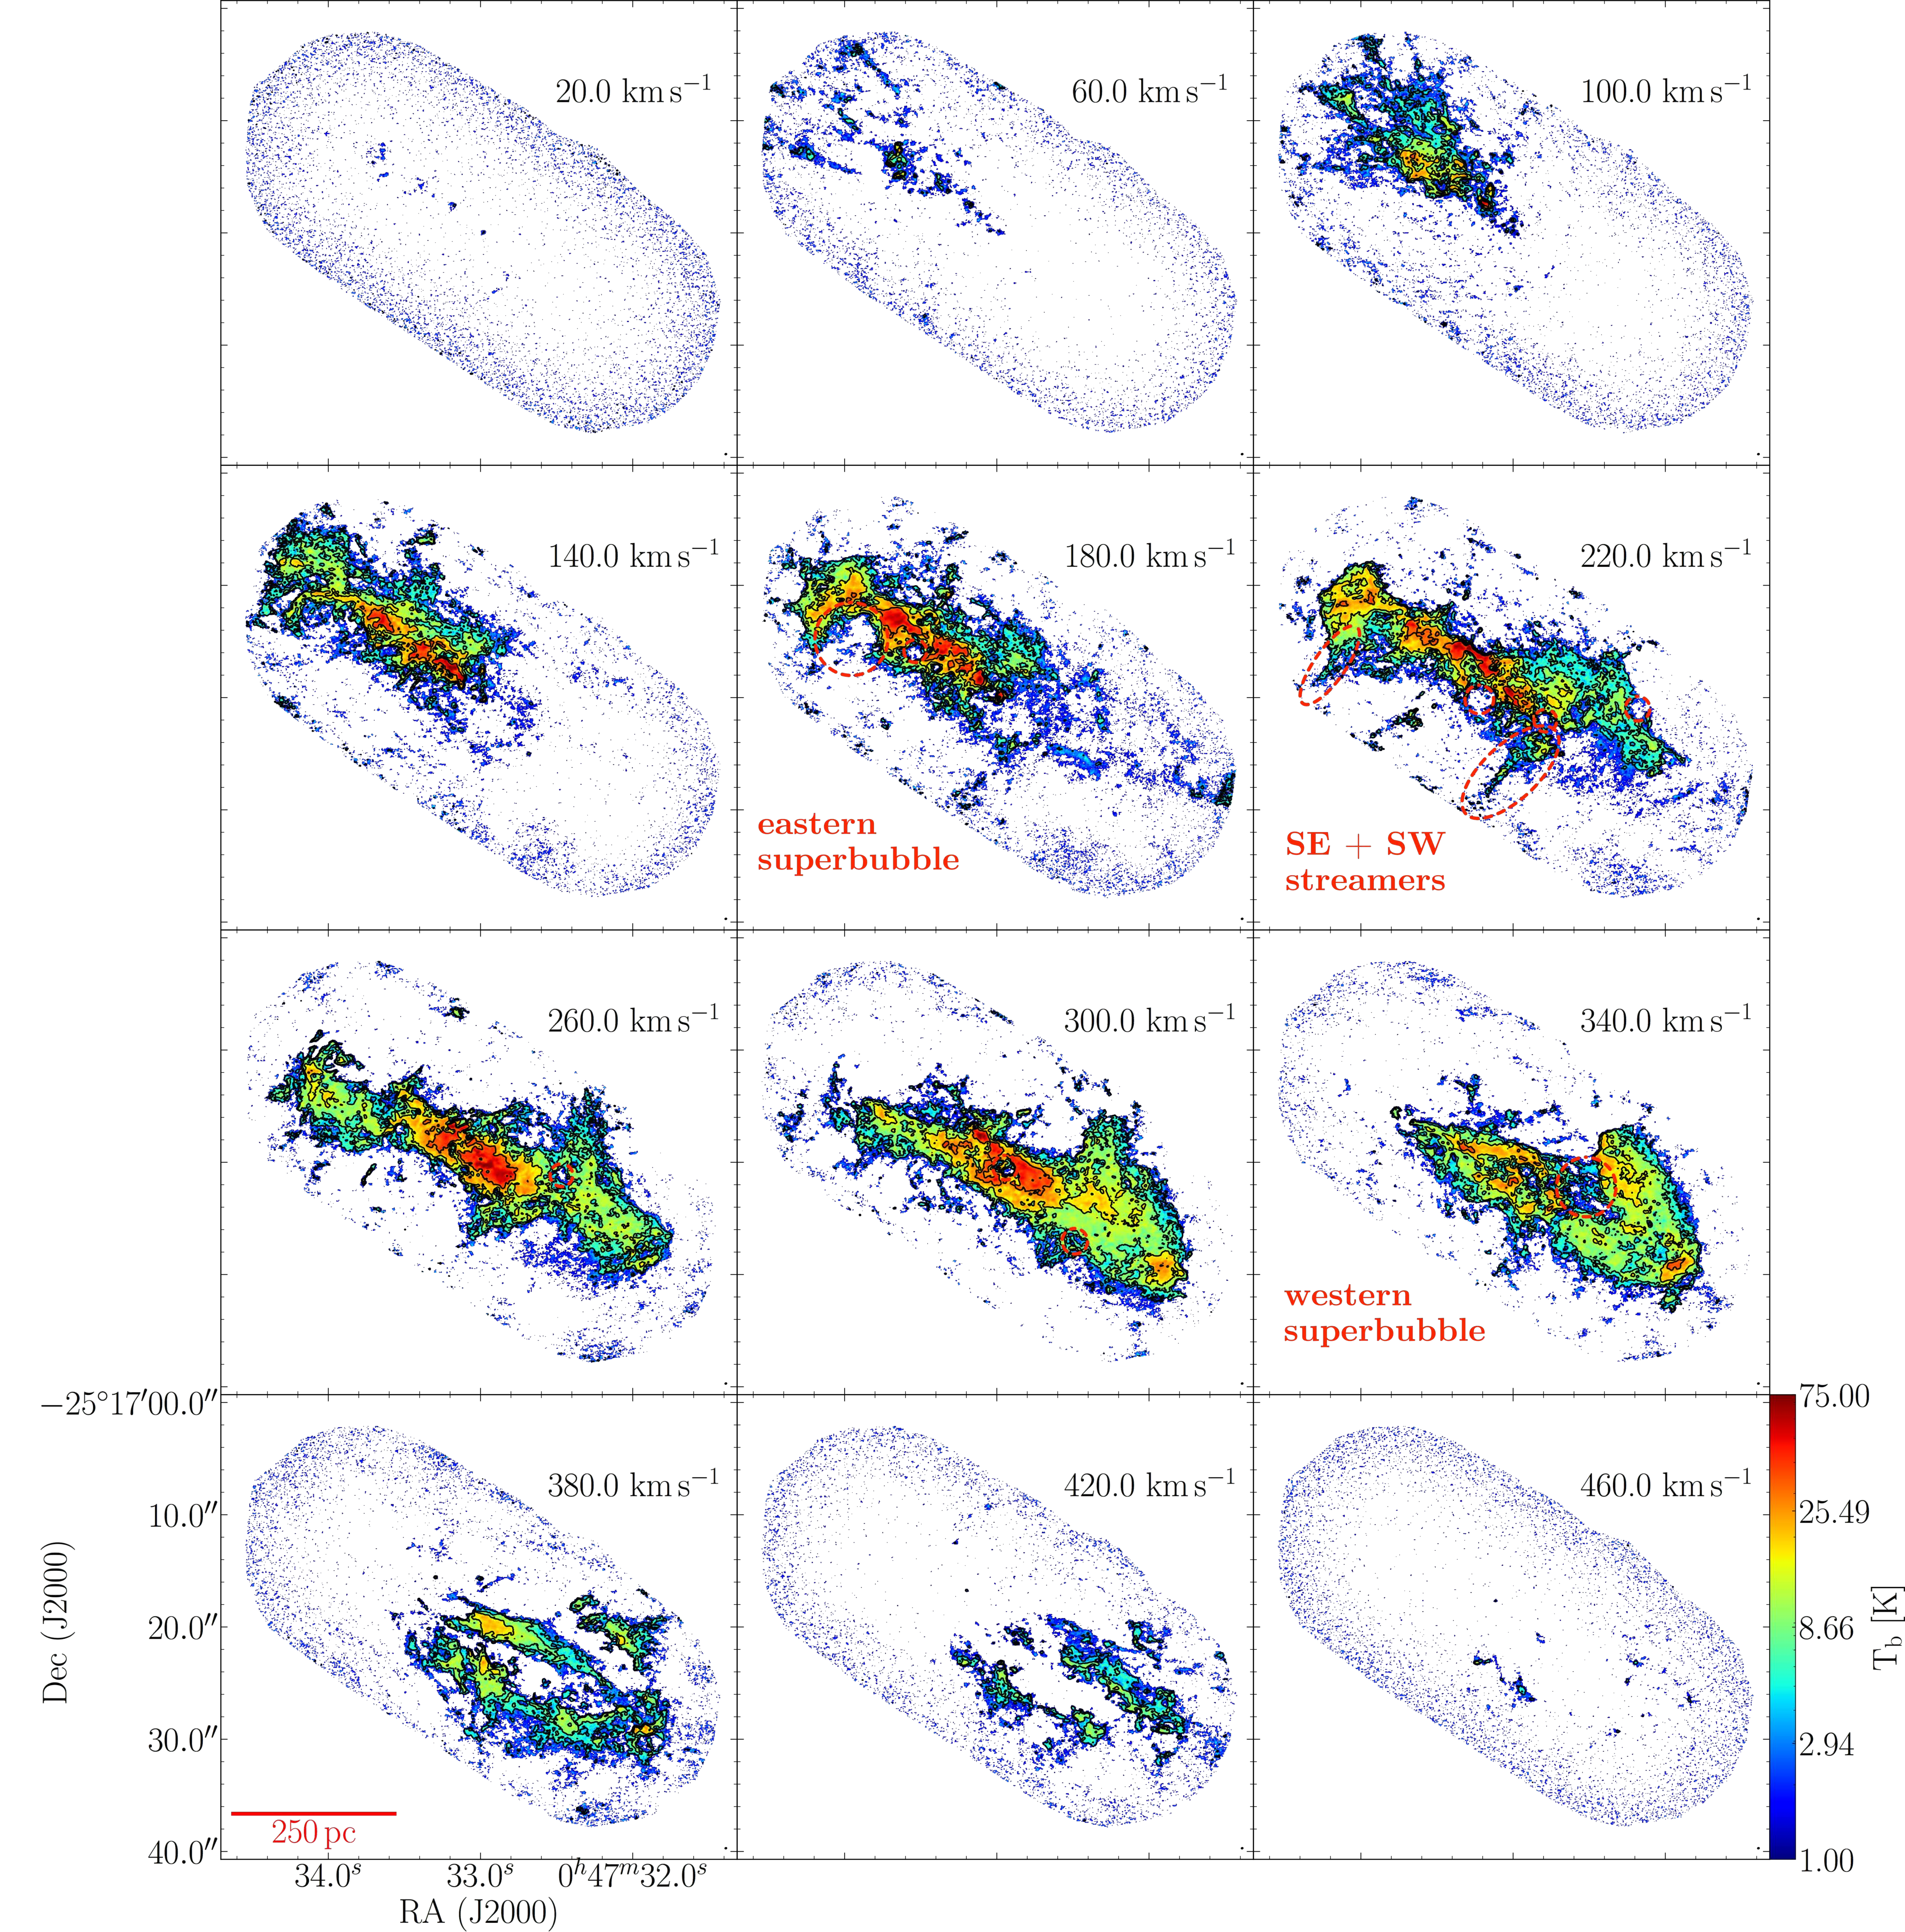
\includegraphics[width=\linewidth]{images/chapters/papers/outflow/outflow_fig1.pdf}
	\caption[NGC253 \co32 channel map]{Channel maps of \co32 in \ngc253. Every $16^{th}$ channel of 2.5\,\kms width is shown with the corresponding line-of-sight velocity ($\mathrm{v}_{sys} = 250$\,\kms) given in the upper right corner of each panel. The synthesized beam of $0.17" \times 0.13"$ is plotted in the lower right corner; it is hardly noticeable due to its small size. Contours are plotted at $10\sigma$, $20\sigma$, $40\sigma$, $80\sigma$ with an RMS noise of $\sigma = 0.37$\,K. Large structures are marked by dashed contours in those panels that show them most clearly. Further new shells are indicated by dashed circles.}
	\label{outflow: figure: CO channel map}
\end{figure*}

\begin{figure}
	\centering
	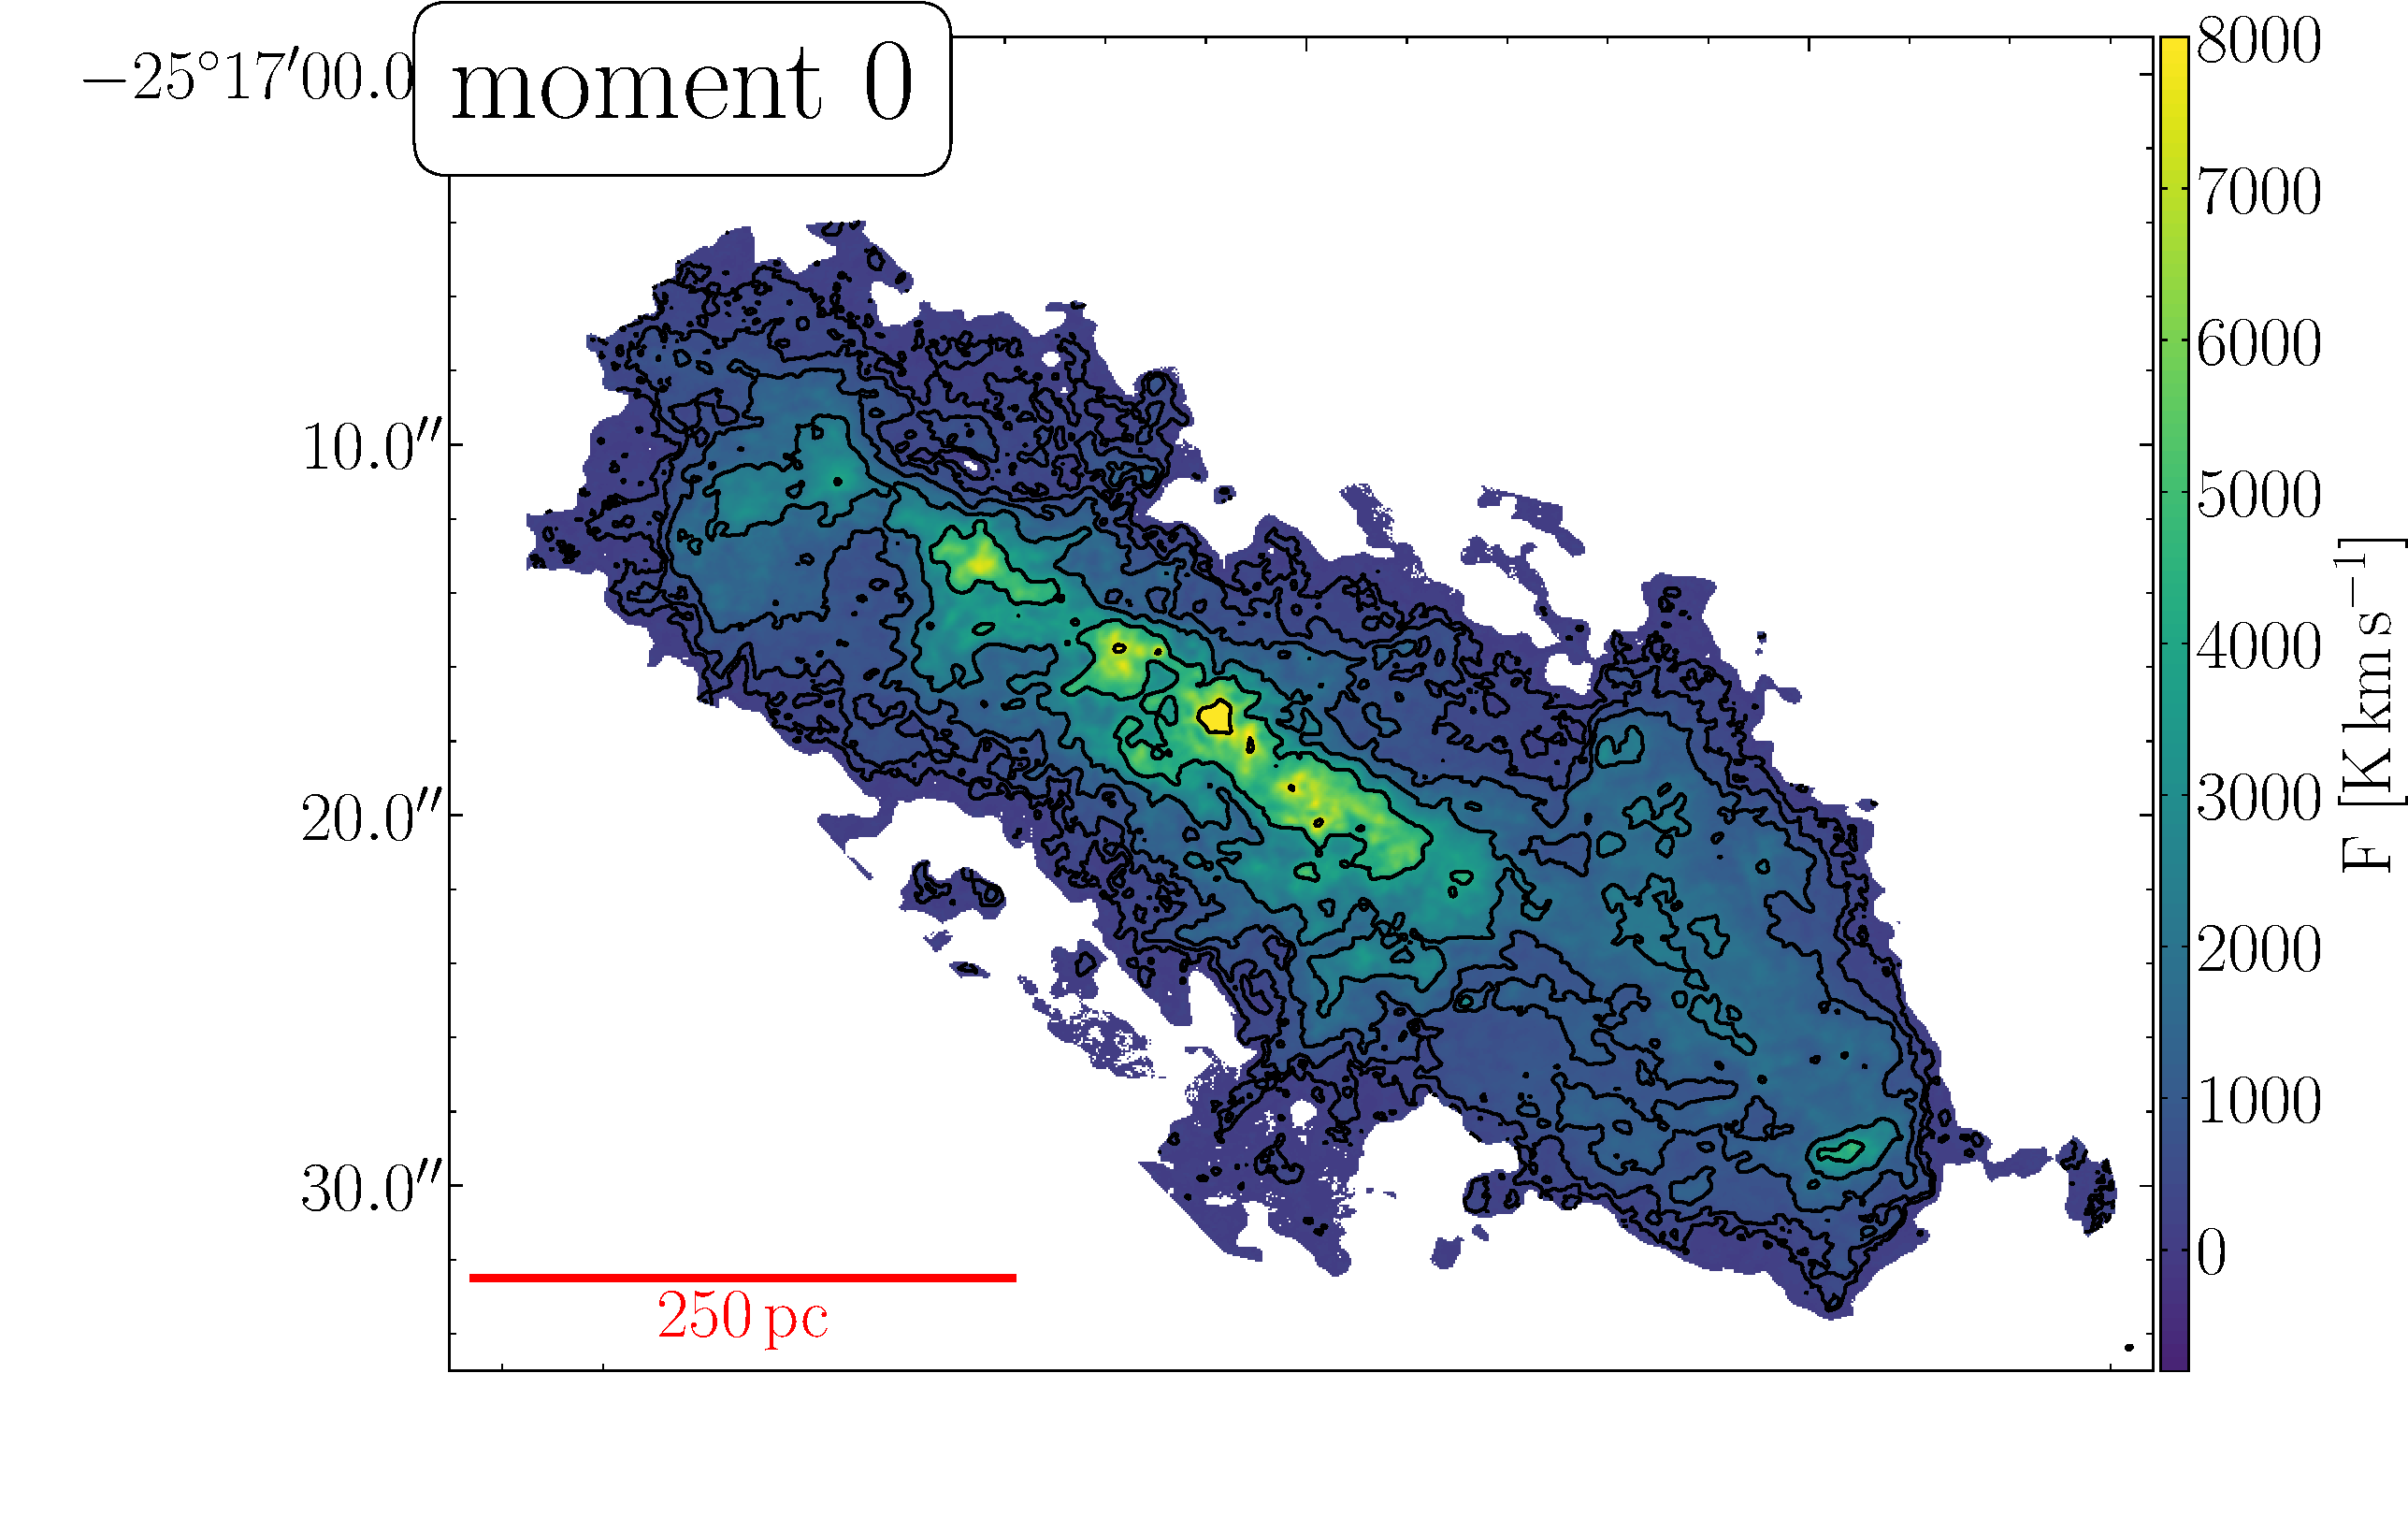
\includegraphics[width=0.6\textwidth]{images/chapters/papers/outflow/outflow_fig2a.pdf}
	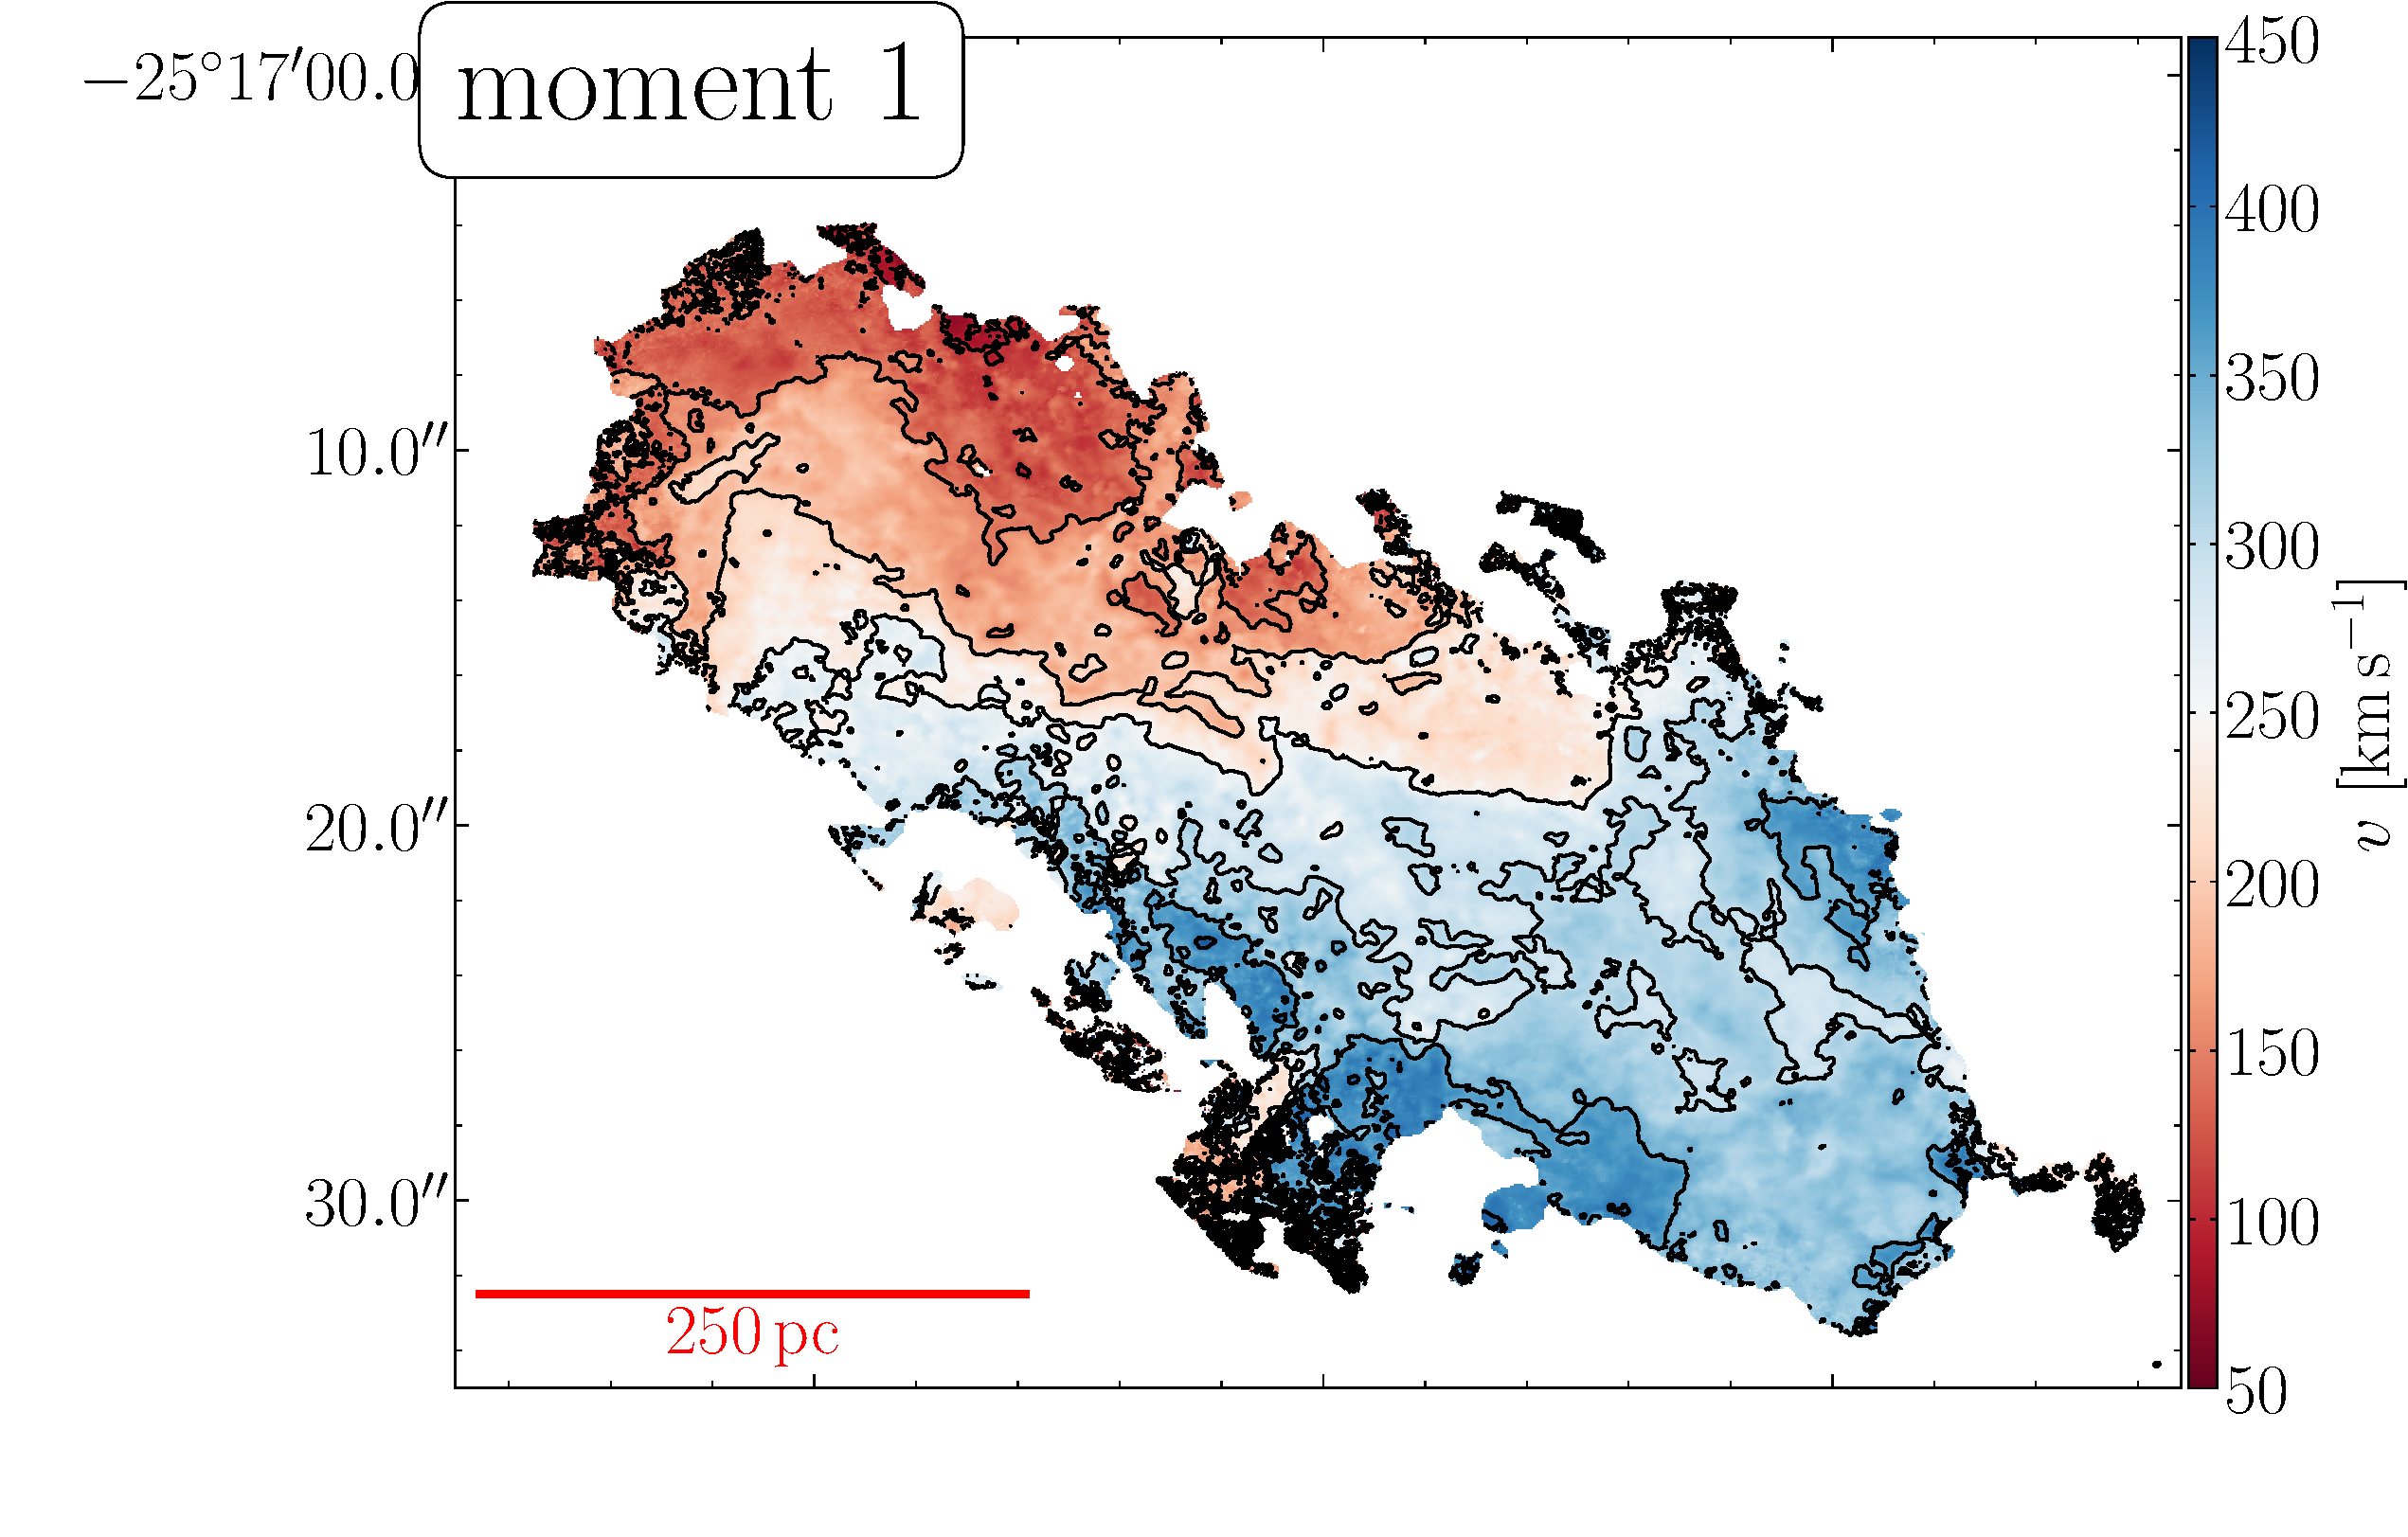
\includegraphics[width=0.6\textwidth]{images/chapters/papers/outflow/outflow_fig2b.pdf}
	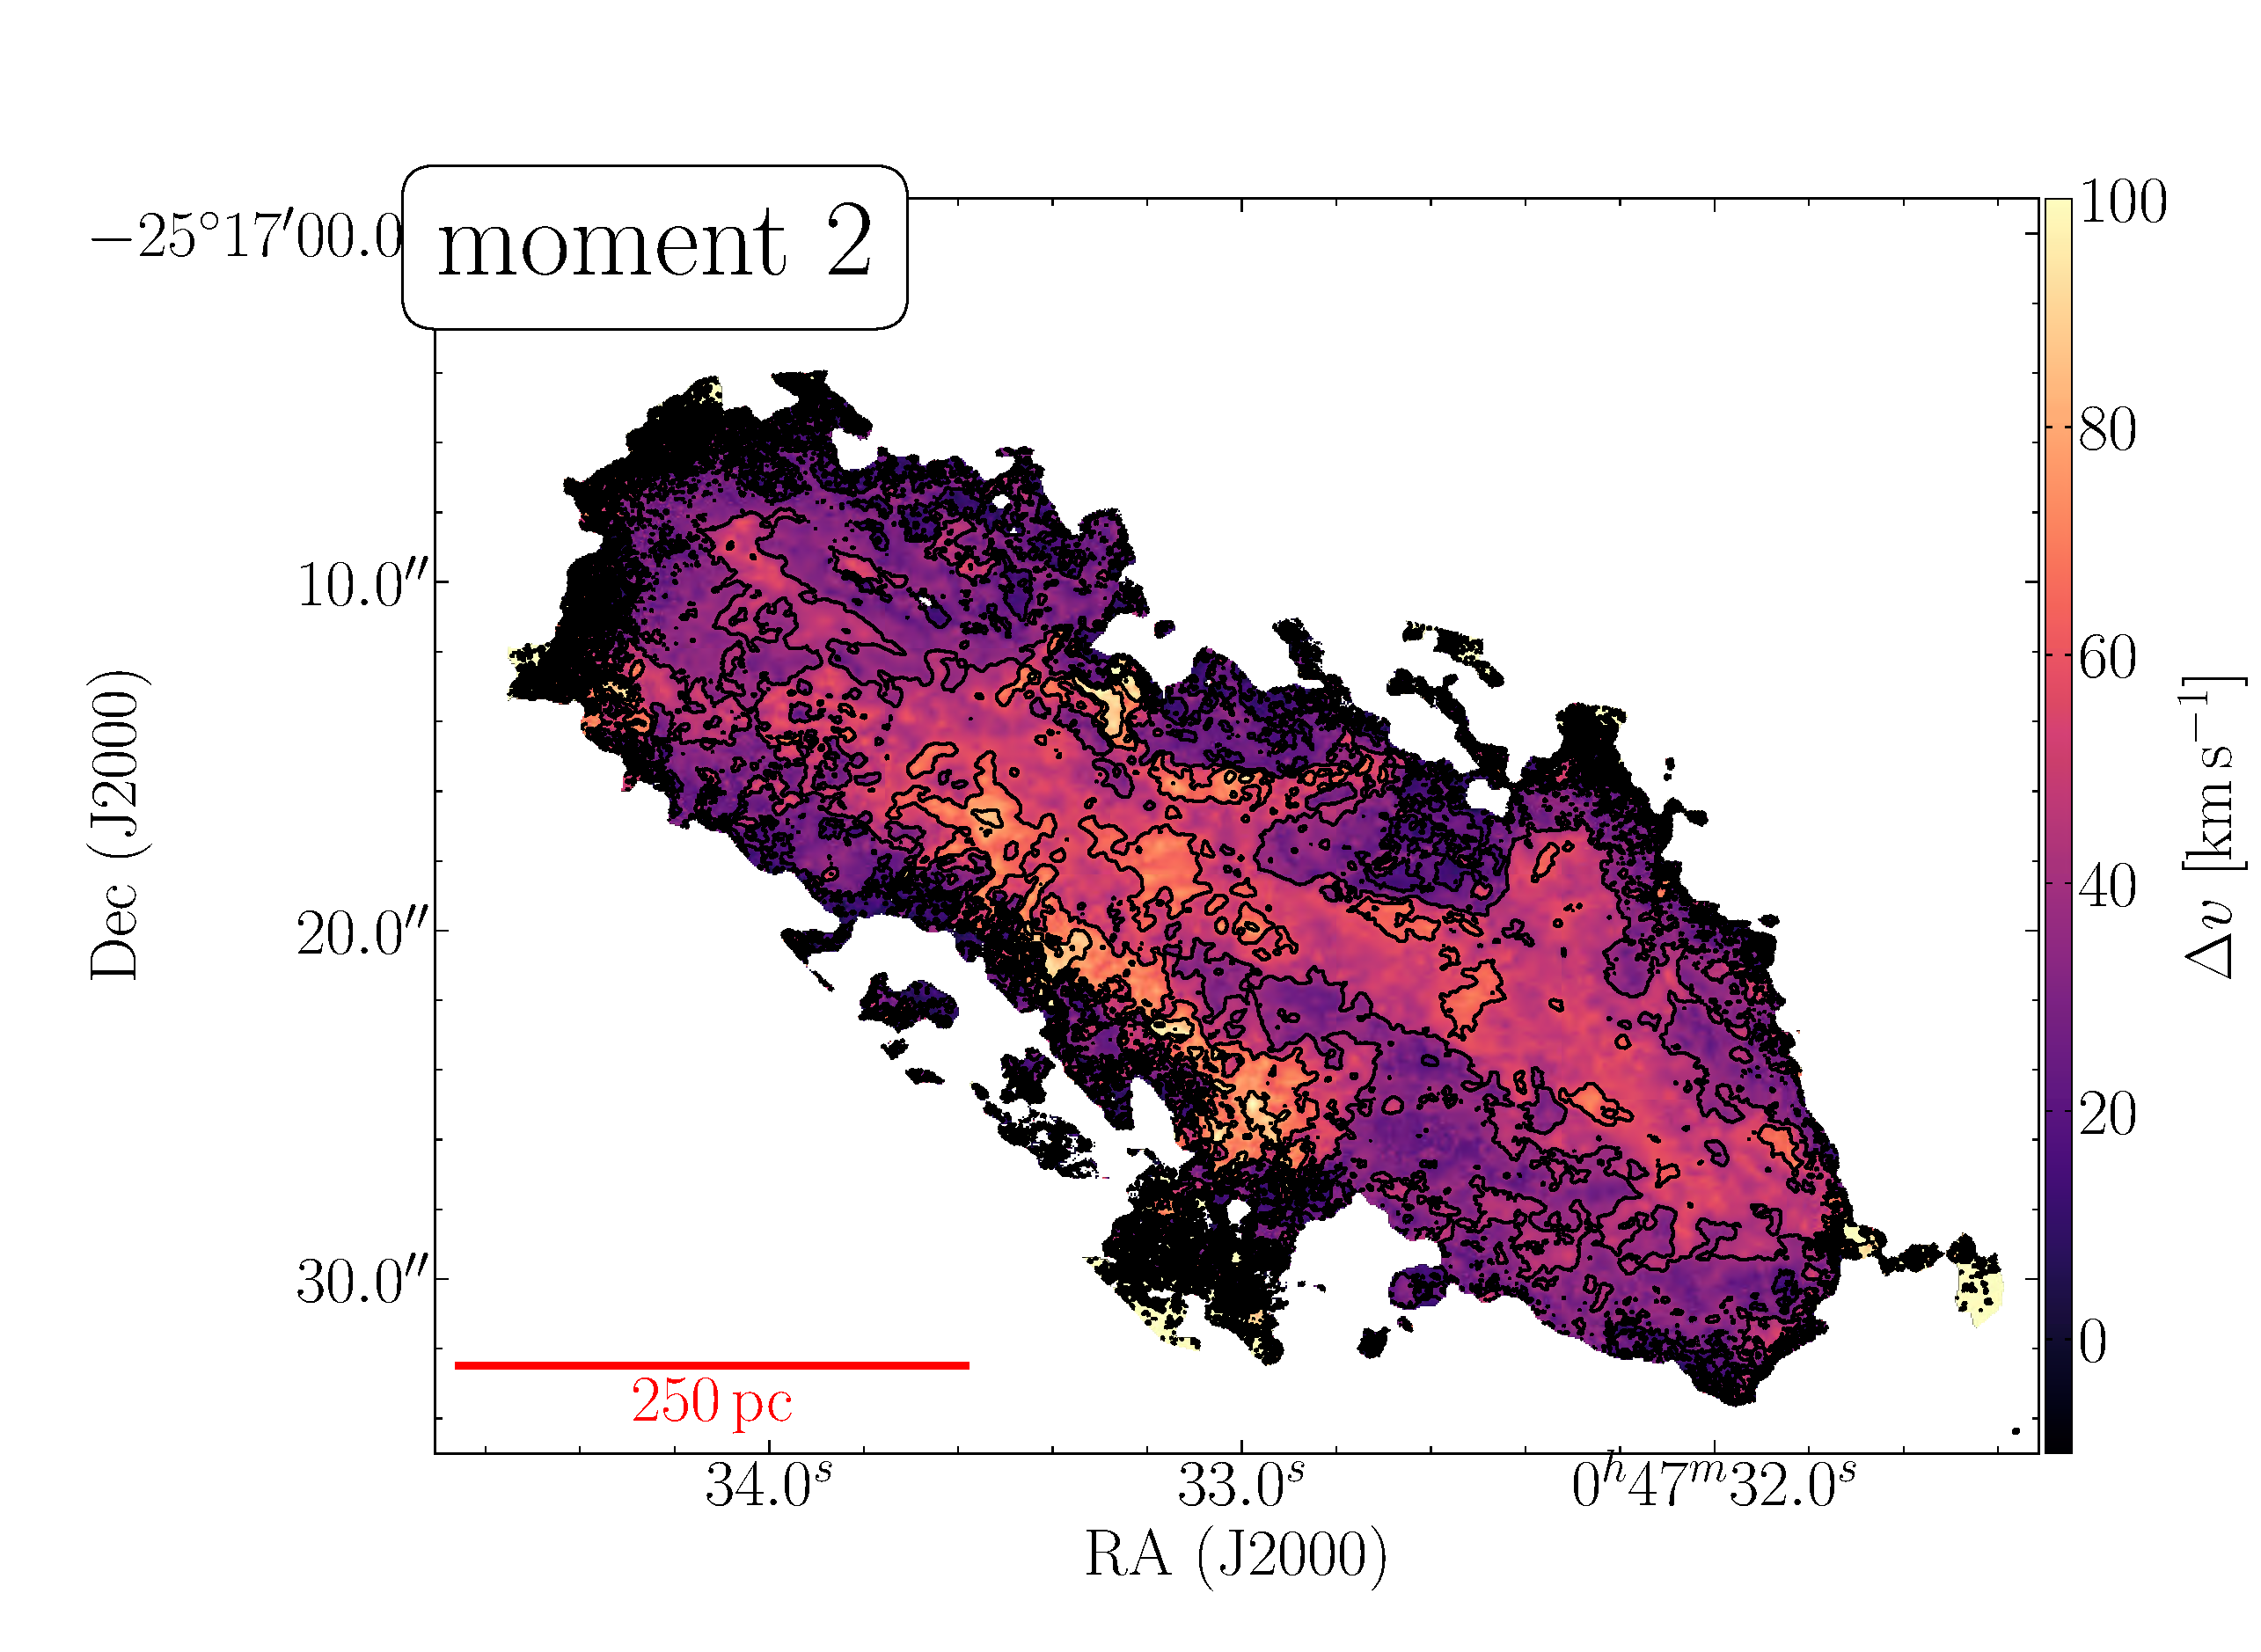
\includegraphics[width=0.6\textwidth]{images/chapters/papers/outflow/outflow_fig2c.pdf}
	\caption[NGC253 \co32 moment maps]{\co32 moment maps of \ngc253. \emph{Top}: Integrated intensity map (moment 0); contours are show from $250 - 8000$\,K\,\kms in factors of two. \emph{middle}: Velocity field (moment 1); contours are shown from 100\,\kms -- 400\,\kms in steps of 50\,\kms. \emph{Bottom}: Moment 2 (corresponding to the velocity dispersion if the line profile would be Gaussian); contours are shown from 0\,\kms -- 100\,\kms in steps of 20\,\kms. The color scale is chosen to saturate a few regions with dispersions $\GTR 100$\,\kms. All maps are generated from the data cube masked a $5\sigma$ threshold per channel and confined to the collapsed clean mask to include only emission that has been processed by the clean algorithm.}
	\label{outflow: figure: CO moment maps}
\end{figure}

\begin{figure}
	\centering
	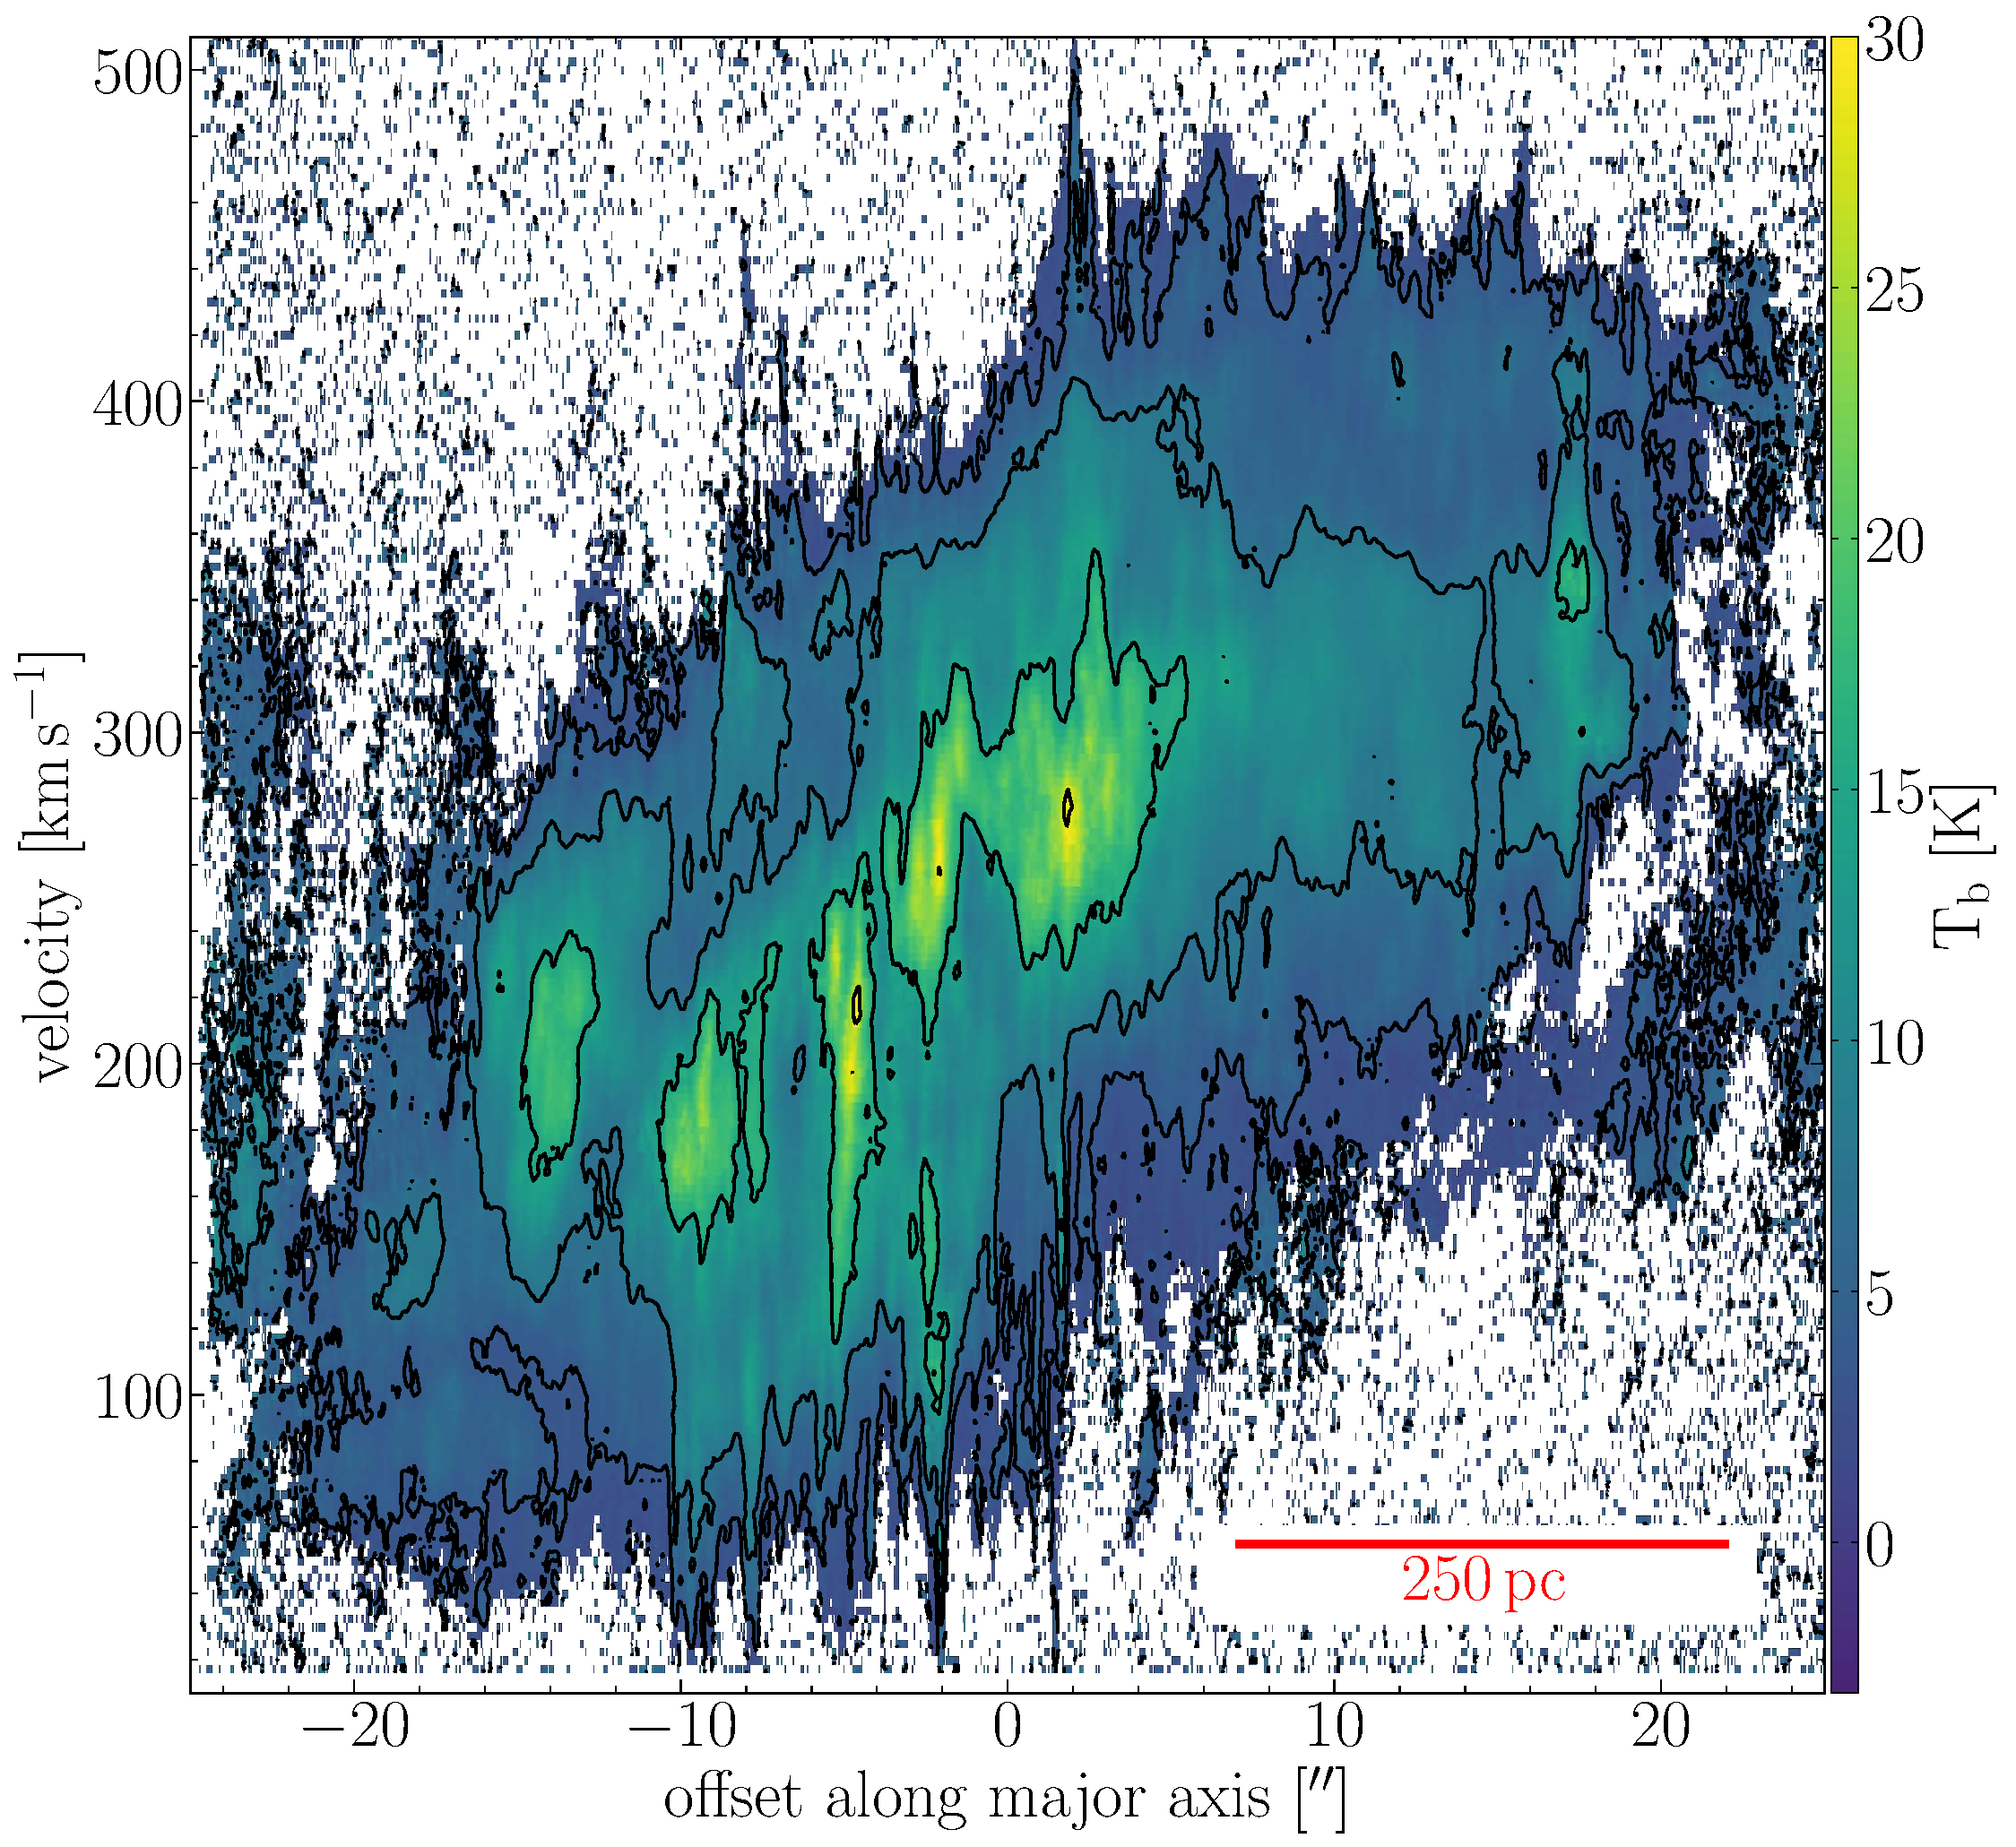
\includegraphics[width=0.6\linewidth]{images/chapters/papers/outflow/outflow_fig3.pdf}
	\caption[NGC253 \co32 position-velocity diagram]{\co32 position-velocity diagram of \ngc253 along the major axis centered on the kinematic center averaged over the full width of the field of view ($\sim 30\arcsec$). Pixel below $3\sigma$ are masked and contours are drawn at $10\sigma$, $20\sigma$, $40\sigma$, $80\sigma$ with an RMS noise of $\sigma = 0.37$\,K. Note the vertical spikes indicating high velocity dispersion due to outflowing gas.}
	\label{outflow: figure: co pV}
\end{figure}

In this section, we present the \co32 data in different representations. Channel maps (Figure~\ref{outflow: figure: CO channel map}), moment maps (Figure~\ref{outflow: figure: CO moment maps}) and a position-velocity (pV) diagram (Figure~\ref{outflow: figure: co pV}) show the spatial and kinematic structures to be discussed and highlight the data quality.

Figure~\ref{outflow: figure: CO channel map} shows channel maps of the image cube. To retain the intrinsic resolution, only every 16$^{th}$ channel (40\,\kms spacing) is shown here. Besides the rotating disk of molecular gas, we clearly detect the prominent south-west (SW) streamer \citep{2017ApJ...835..265W} in the range $180 - 250$\,\kms (Figure~\ref{outflow: figure: CO channel map}, panels 220\,\kms and 260\,\kms). Additional gas streamers are apparent between $\sim 60$\,\kms and $\sim 350$\,\kms towards north and south of the disk as can be seen for example in the panels at 260\,\kms or 340\,\kms. Several notable molecular shells are present between 180\,\kms and 340\,\kms. Beside the (super-)shells at the eastern (left) and western (right) edge of the map that have been previously identified by \citet{2006ApJ...636..685S} and \citet{2013Natur.499..450B}, further smaller shell--like structures are located along the molecular disk.

We calculate image moments (Figure~\ref{outflow: figure: CO moment maps}) with \texttt{immoments} in \textsc{casa} for emission above $5\sigma$ for the moment 0 (integrated intensity) map, the moment~1 (intensity-weighted line-of-sight velocity) and moment~2 (intensity-weighted velocity dispersion) maps. Note that due to the complex line shapes, the moment~2 map does not directly correspond to velocity dispersion which is only the case for Gaussian line profiles. The maps are further constrained to the region defined by the collapsed clean mask to limit them to emission that has been processed by the clean algorithm.

Figure~\ref{outflow: figure: co pV} shows the kinematic structure of \ngc253 as a pV diagram along the major axis of the disk ($\mathrm{PA} = 55^\circ$) averaged over the full width of the field of view ($\sim 30\arcsec$) centered on the kinematic center. The pV cut shows several high velocity dispersion structures extending from a rotating disk, indicative of outflows.


%%%%%%%%%%%%%%%%%%%%%%%%%%%%%%%%%%%%%%%%%%%%%%%%%%%%%%%%%%%%%%%%%%%%%%%%%%%%%%%%%%%%%%%%%%%%%%%%%%%%
%%%%%%%%%%%%%%%%%%%%%%%%%%%%%%%%%%%%%%%%%%%%%%%%%%%%%%%%%%%%%%%%%%%%%%%%%%%%%%%%%%%%%%%%%%%%%%%%%%%%

\section{Separating disk and non-disk emission}
\label{outflow: section: disk separation}


%%%%%%%%%%%%%%%%%%%%%%%%%%%%%%%%%%%%%%%%%%%%%%%%%%%%%%%%%%%%%%%%%%%%%%%%%%%%%%%%%%%%%%%%%%%%%%%%%%%%

\subsection{Separating disk and non-disk emission in position-position-velocity space}
\label{outflow: subsection: ppV separation}

Our goal is to account for all the molecular wind, separating outflowing molecular gas from foreground or background disk emission. A clean separation in 2D position-position space cannot be easily accomplished due to the inclination of $78^\circ$ of \ngc253. At this high inclination, outflows and disk emission are co-spatial in projection. Kinematic information from line-of-sight velocities, however, makes it possible to disentangle the outflow. Note that this becomes increasingly difficult as the velocity vector aligns with the plane of the sky, resulting in line-of-sight velocities that are systemic. From H$\alpha$ kinematic modeling the \ngc253 outflow is approximately bi-conical with an axis normal to the disk and an opening angle of $\sim60^\circ$ \citep{Westmoquette:2011bp}, and thus the range of possible projection angles is large (see \citealt{2015ApJ...801...63M} for a sketch). Note that because the cone opening angle is larger than the angle between the axis of the cone and the plane of the sky, gas in the approaching and receding cones can have both blue- and red-shifted velocities with respect to systemic.

The launching of molecular gas occurs within the disk through star formation feedback, thus the outflows originate from the same location in position-position-velocity (ppV) space as disk molecular clouds. Outflows will therefore blend into the disk near their launching sites, which makes disentanglement increasingly difficult closer to the starburst region.

The complexity of systematically separating emission corresponding to the disk and the outflow in ppV space is challenging. Algorithmically, this separation is simpler in a lower dimensional space, obtained by slicing the data cube into a collection of 2D position-velocity diagrams. In what follows we identify kinematic components in these diagrams, which then we project back to 3D ppV space. In order to avoid introducing biases we model the large-scale disk velocity field and use this model as the basis of the kinematic separation.

%%%%%%%%%%%%%%%%%%%%%%%%%%%%%%%%%%%%%%%%%%%%%%%%%%%%%%%%%%%%%%%%%%%%%%%%%%%%%%%%%%%%%%%%%%%%%%%%%%%%

\subsection{Definition of components}
\label{outflow: subsection: definition disk non-disk}

Images of the center of \ngc253 on large scales show an elongated gas structure (Figure~\ref{outflow: figure: CO moment maps} top) with a regular velocity field (Figure~\ref{outflow: figure: CO moment maps} middle) that roughly matches a rotating disk disturbed by streaming motions from a bar \citep[e.g.][]{2004ApJ...611..835P}. The elongated gas structure is consistent with a highly inclined disk of molecular gas, or possibly a ring-like structure as observed in other galaxies \citep[for example, NGC\,1512, NGC\,1808;][]{2016ApJ...823...68S,2018ApJ...857..116M}. 
Similar structures break up at higher spatial resolution into two embracing spiral arms or complex non-closed orbits in the Milky Way center \citep{2015MNRAS.453..739K,2016MNRAS.457.2675H,2018MNRAS.481....2S}. 

Superimposed on this large scale structure, there are smaller features that are not part of the large-scale pattern of rotation and streaming motions. Some of them have high aspect ratios in channel maps and line-of-sight velocity gradients, both typical for outflows. Local deviations from the large-scale velocity field can also be due to infalling gas, or clumps of gas that do not follow the global pattern due perhaps to a cloud-cloud collision.

Henceforth, we will refer to the bulk of the molecular gas that moves according to the large-scale velocity field in the central regions of \ngc253 as the \emph{disk}. We assume this large-scale velocity field consists of rotation and streaming motions. The term \emph{non-disk} refers to any gas that is not following the ppV structure of the disk. By this definition, non-disk gas encompasses material from features that may be attributed to a variety of physical processes, including outflow and infall. 

Structures of outflowing gas are frequently referred to by names that describe their kinematic or spatial appearance, such as ``streamer''. We will use the term outflow to denote localized structures with morphology and kinematics consistent with gas moving away from the disk, as inferred from their location in ppV space. Typical signatures are a velocity that is inconsistent with rotation in the plane of the disk, and a high aspect ratio oriented roughly perpendicular to the disk major axis. Note that similar kinematic and structural properties can arise in infalling gas clouds. We will assume that all molecular gas with these characteristics is outflowing, which is likely the case for the majority of the material in \ngc253.  

%%%%%%%%%%%%%%%%%%%%%%%%%%%%%%%%%%%%%%%%%%%%%%%%%%%%%%%%%%%%%%%%%%%%%%%%%%%%%%%%%%%%%%%%%%%%%%%%%%%%

\subsection{Position-velocity slicing}
\label{outflow: subsection: slicing}

Kinematic analyses typically depend on high signal-to-noise ratios (SNR) because faint features can easily drown in noisy spectra. As a trade-of between necessary high SNR and also trying to include as much faint emission as possible, we conduct the following analysis on data cubes masked at the $5\sigma$ level (cf. Table~\ref{outflow: table: used datasets}).

We split the ppV cubes into position-velocity (pV) slices along the major axis of \ngc253 as shown in Figure~\ref{outflow: figure: slice positions}. The slices assume the kinematic center is $\alpha,\delta = 00^h47^m33.134^s, -25^\circ17^m19.68^s$ \citep{MullerSanchez:2010dr}, and are oriented along the major axis of the projected CO emission with $\mathrm{PA} = 55^\circ$. The area sliced is chosen to cover the region for which we have overlapping \co10, (2--1) and (3--2), and also cover the full length of the SW streamer outflow feature \citep[17.5\arcsec,][]{2017ApJ...835..265W}.

These requirements are fulfilled by slices of $50\arcsec$ (850\,pc) length (major axis) and covering $50\arcsec$ (850\,pc) along the minor axis (Figure~\ref{outflow: figure: slice positions}). To reduce the problems introduced by splitting features across slices, each slice is $5.0\arcsec$ (85\,pc) wide, and we overlap slices by half their width ($2.5\arcsec$, 42\,pc). A sample pV diagram is shown in Figure~\ref{outflow: figure: sample slice} for the central slice, which runs along the major axis (offset $0.0\arcsec$). A complete set of pV diagrams is given in appendix~\ref{appendix: outflow: all pVs}. The resolution differences between our three transitions, a factor of $\sim 100$ in beam solid angle, are apparent in Figure~\ref{outflow: figure: sample slice}. In the high angular resolution \co32, small features with large linewidth are common. These features are blurred out in the lower resolution \co10 and (2--1).

\begin{figure}
	\centering
	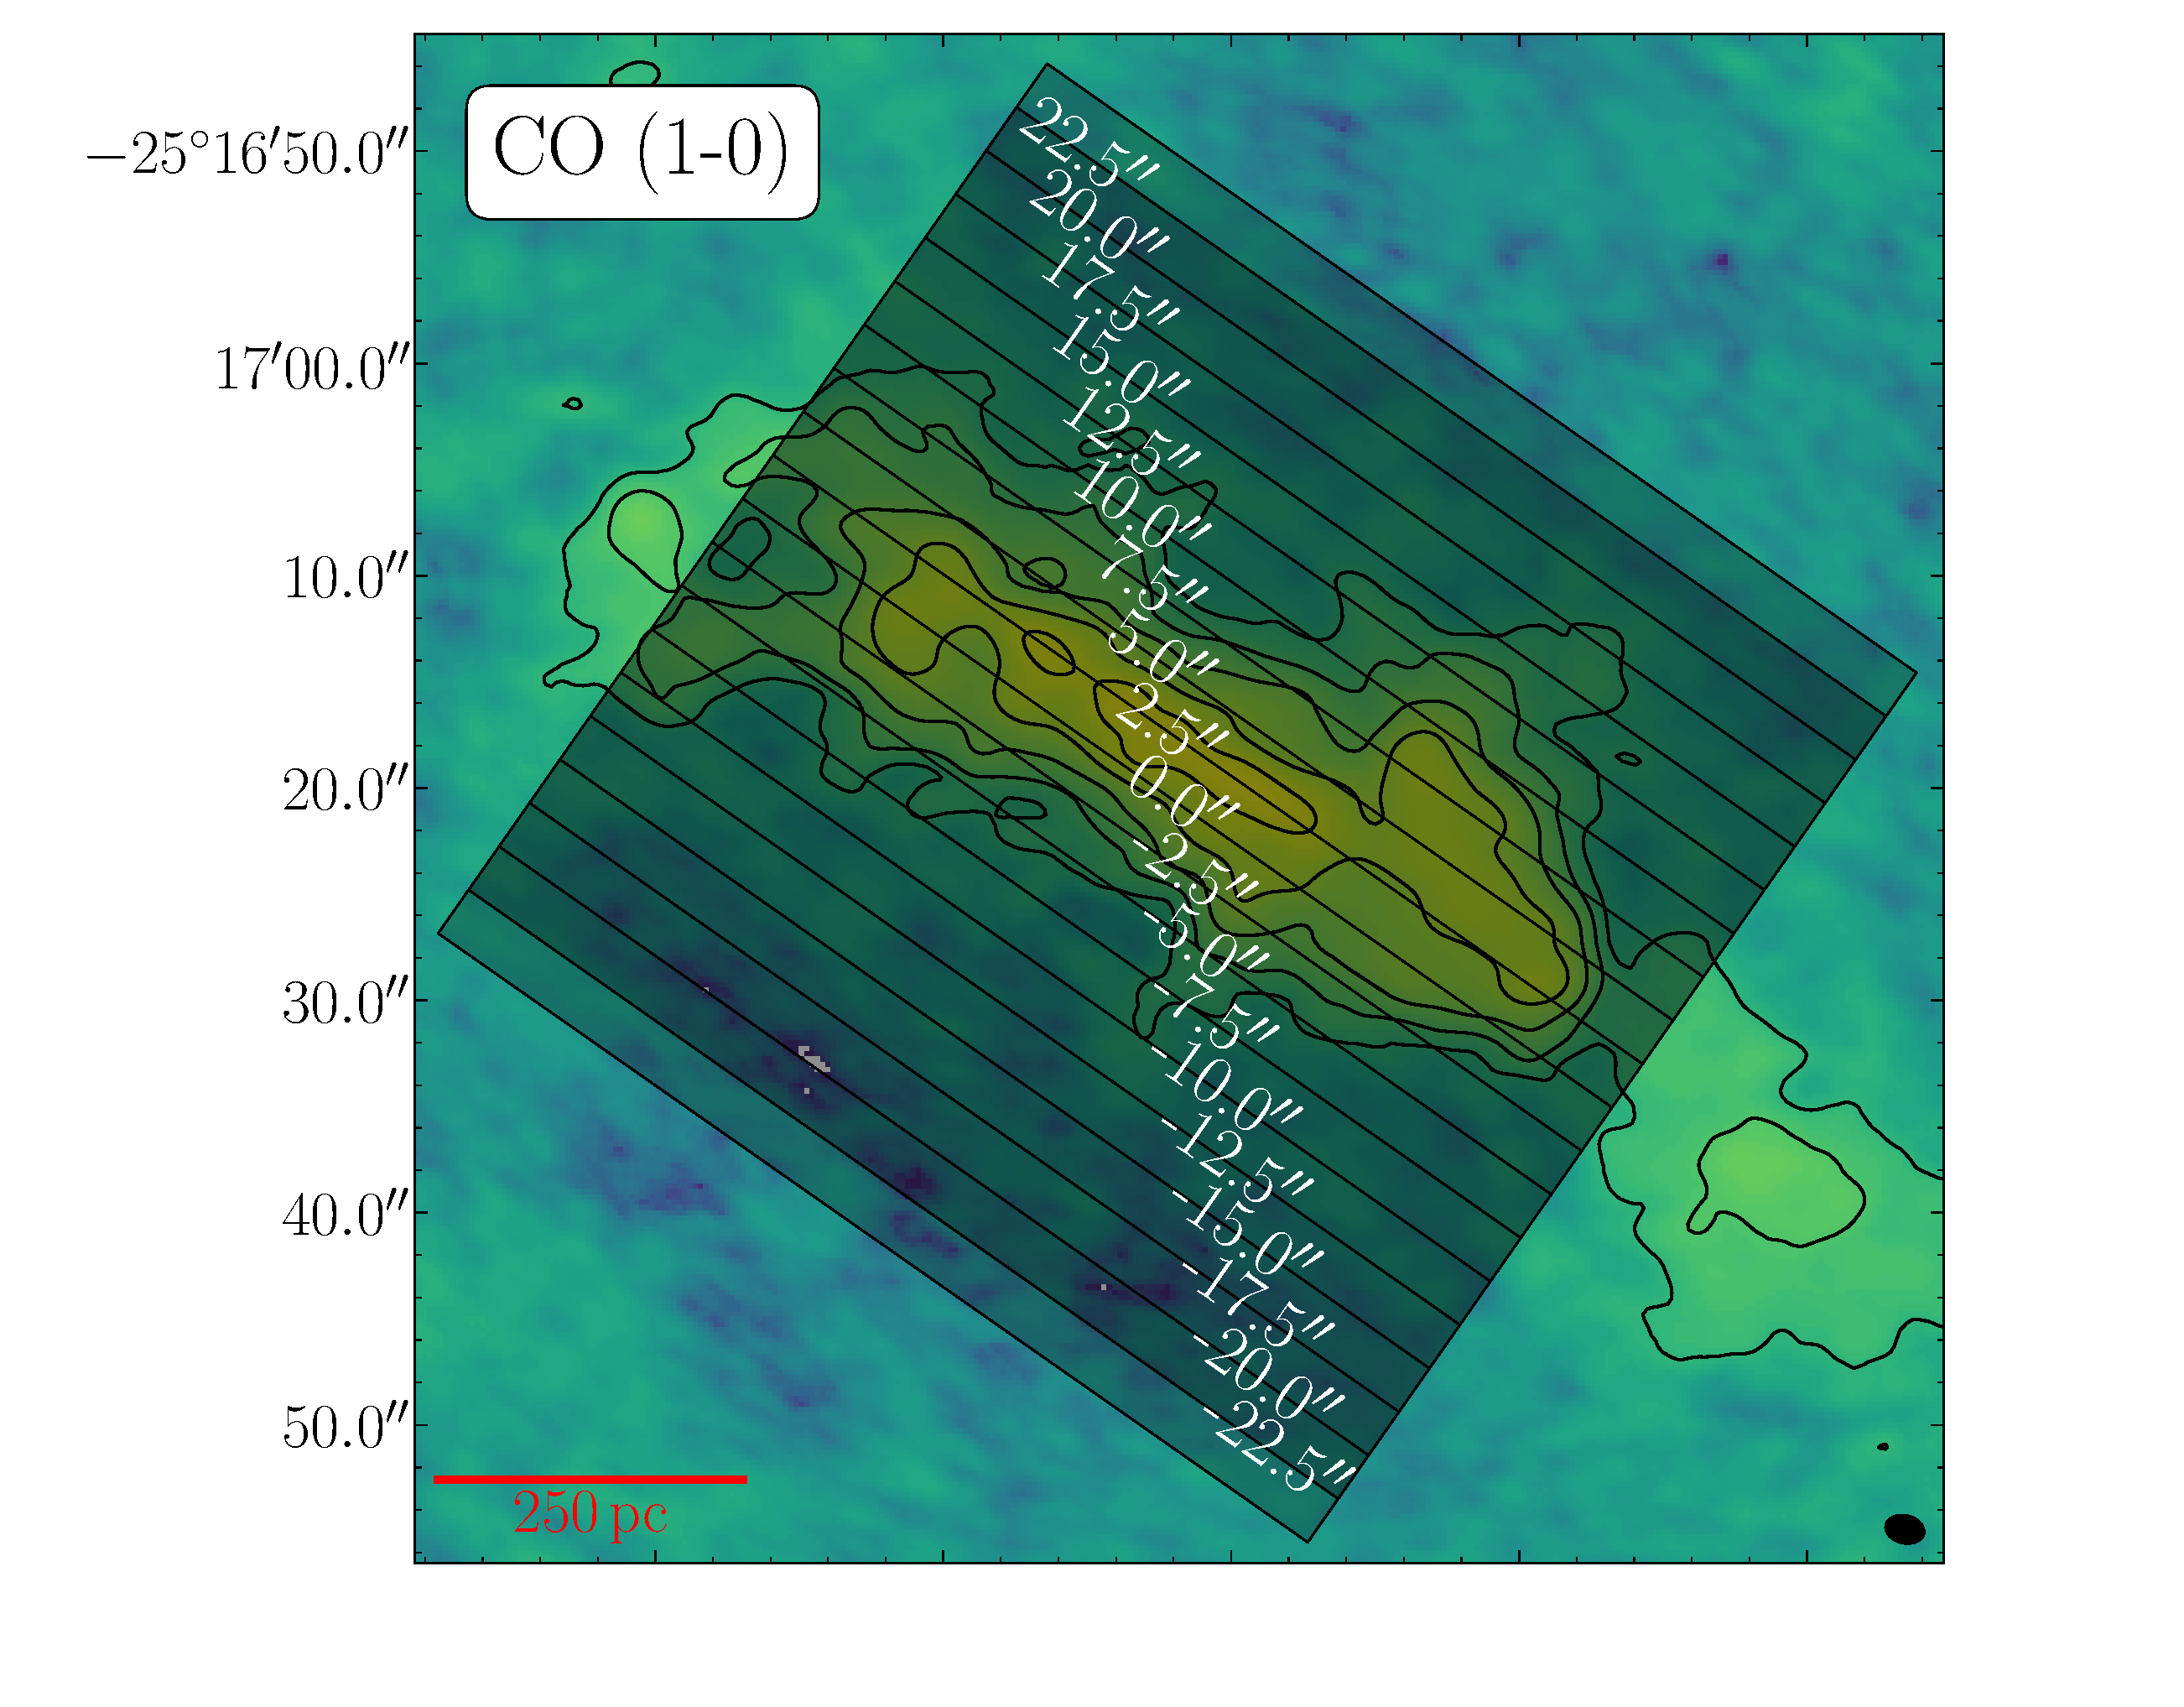
\includegraphics[width=0.6\textwidth]{images/chapters/papers/outflow/outflow_fig4a.pdf}
	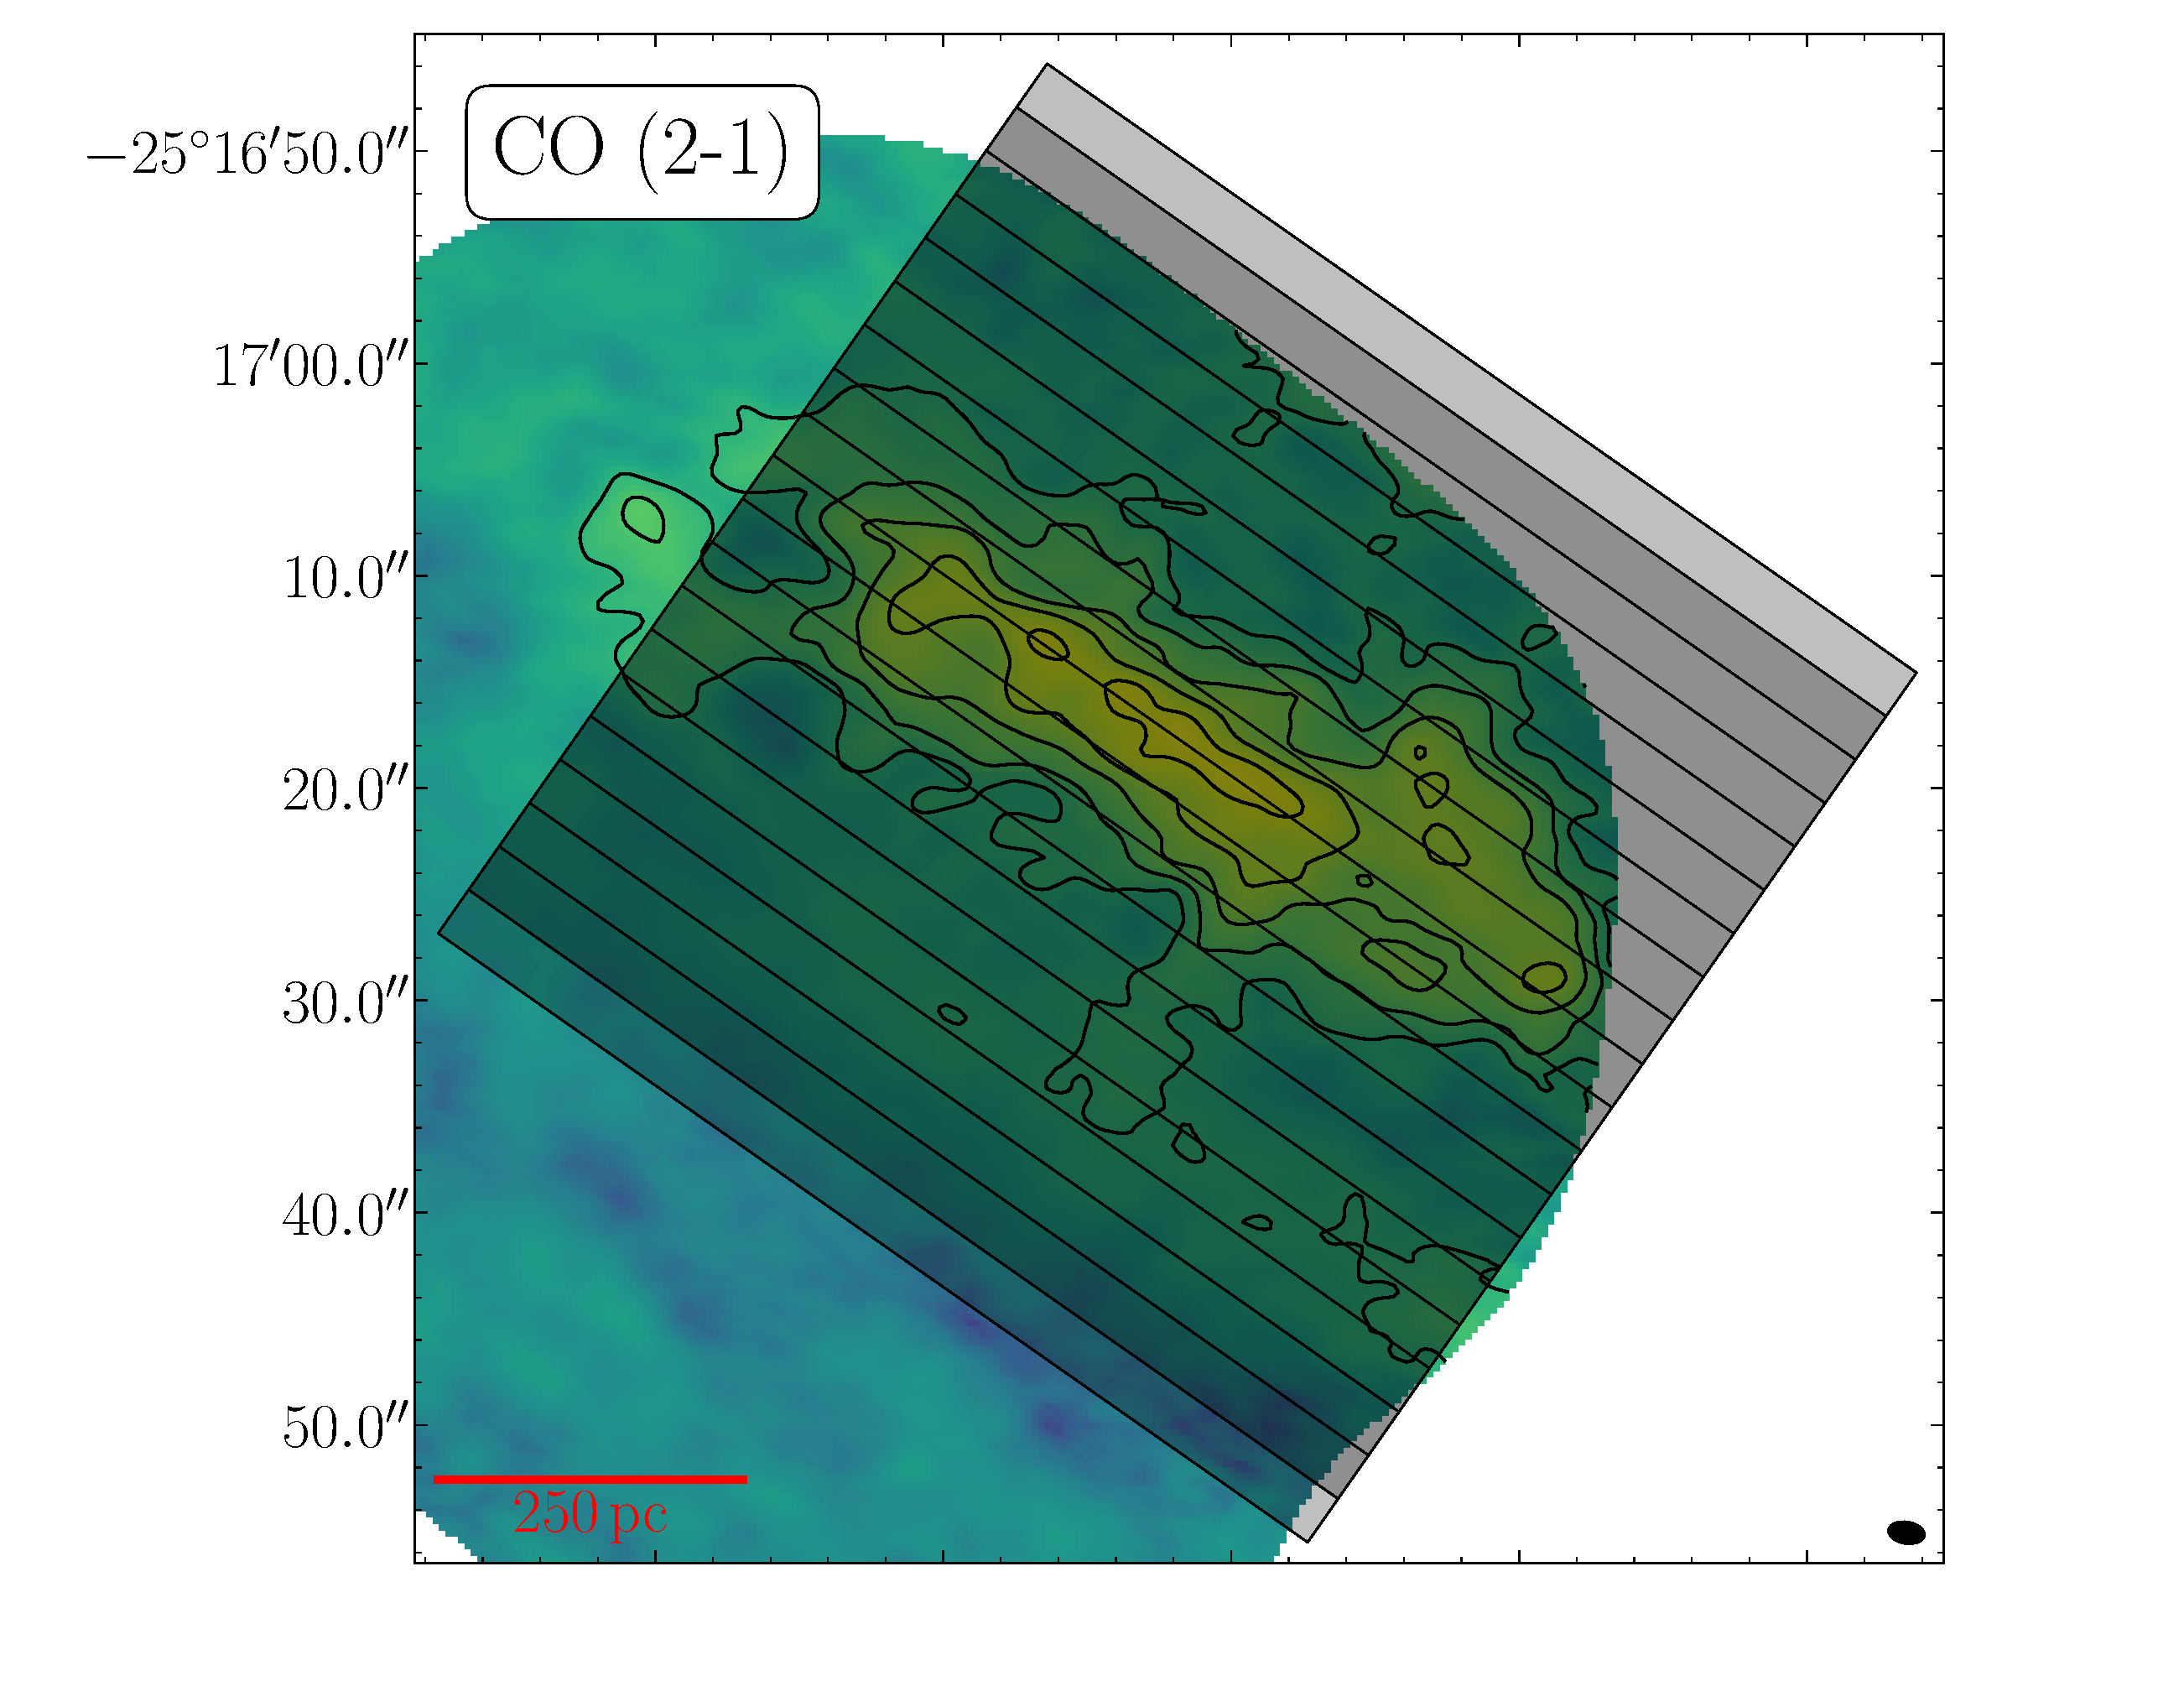
\includegraphics[width=0.6\textwidth]{images/chapters/papers/outflow/outflow_fig4b.pdf}
	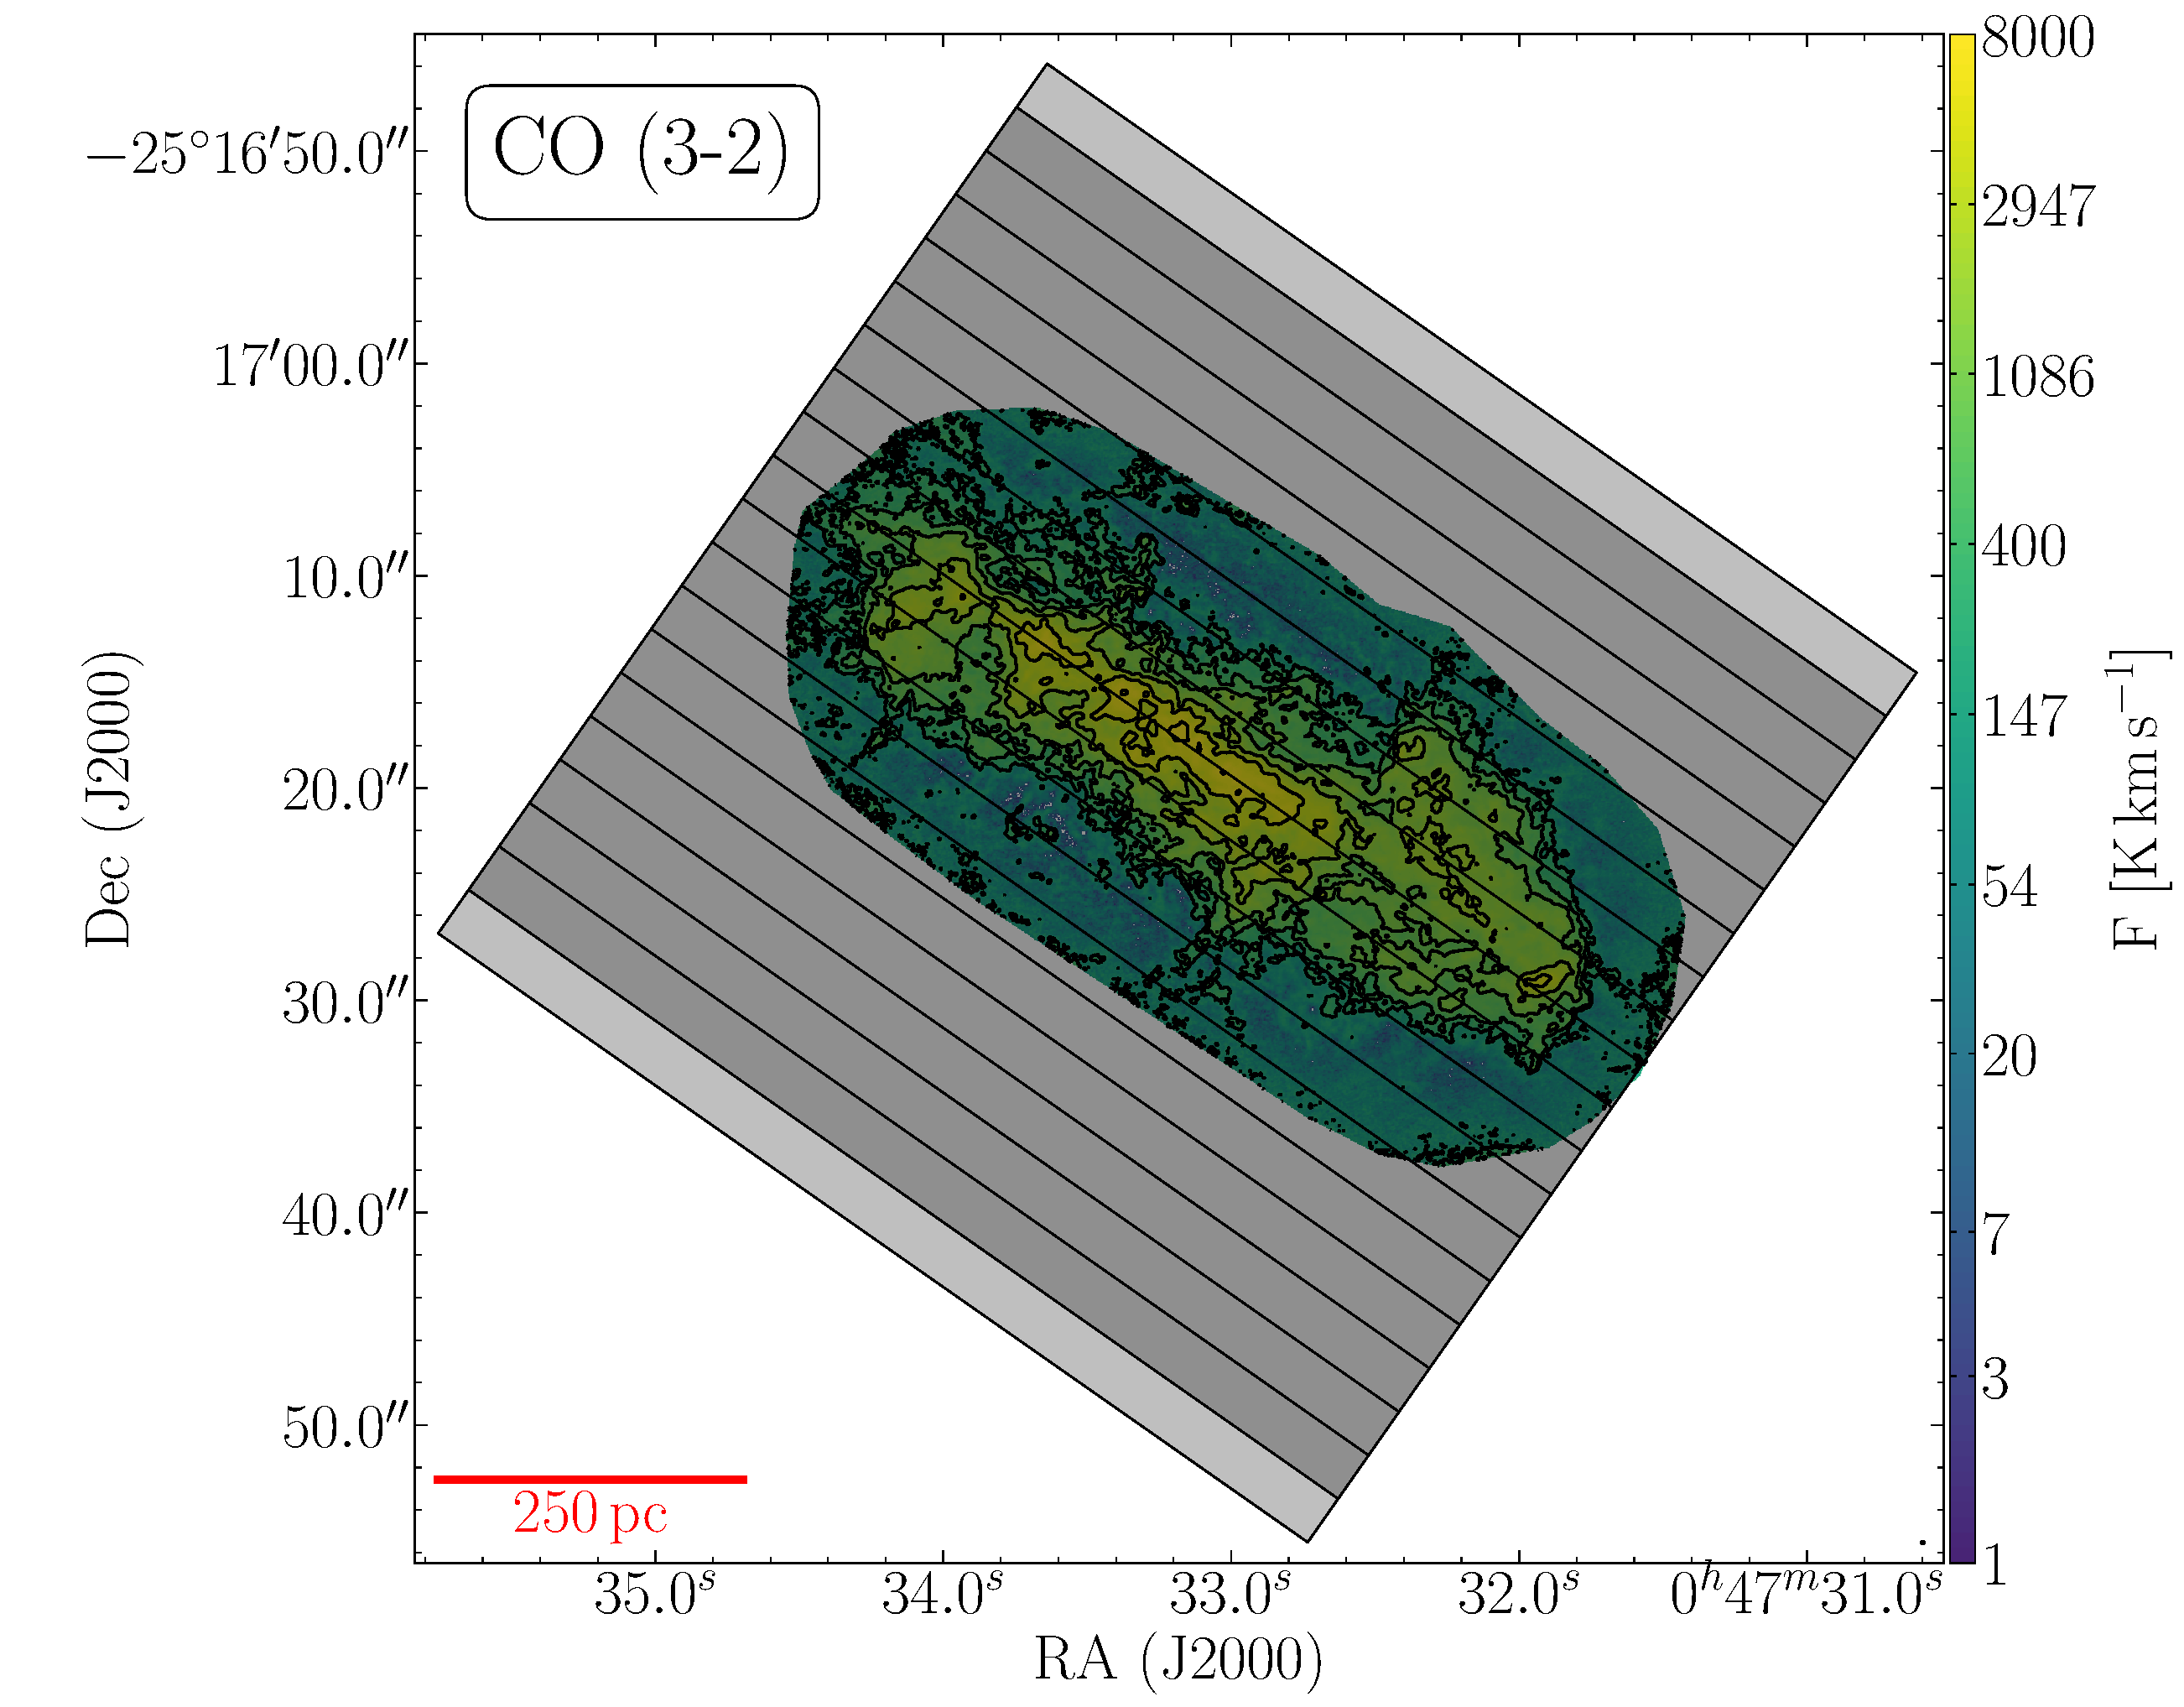
\includegraphics[width=0.6\textwidth]{images/chapters/papers/outflow/outflow_fig4c.pdf}
	\caption[Outline of pV slicing]{Size and orientation of the position-velocity slices overlaid on the integrated intensity image of \co10 (top), \co21 (middle) and \co32 (bottom). Each slice is $5.0\arcsec$ wide and overlaps adjacent slices by $2.5\arcsec$.}
	\label{outflow: figure: slice positions}
\end{figure}


%%%%%%%%%%%%%%%%%%%%%%%%%%%%%%%%%%%%%%%%%%%%%%%%%%%%%%%%%%%%%%%%%%%%%%%%%%%%%%%%%%%%%%%%%%%%%%%%%%%%

\subsection{Modeling the disk}

We derive a model for the velocity of the disk component from the \co10 observations using the kinematic fitting tool \texttt{diskfit} \citep{2007ApJ...664..204S,2010MNRAS.404.1733S,2015arXiv150907120S}. Because the \co10 observations cover the largest area among our observations, we use them to derive the model; the additional information provided by the \co21 and/or \co32 data is negligible in terms of the bulk motions of the gas. We obtain a \co10 velocity field by computing the first moment of the cube after masking it at $20\sigma$ (1.26\,K), in order to represent the velocity of the bright emission.
We show the details of the fit parameters and a comparison to the \co10 velocity field in Appendix~\ref{appendix: outflow: model}.

In each pV slice, we use the velocity profile of the \texttt{diskfit} model to define the local disk velocity. We consider the CO emission consistent with the disk component of the emission when the velocity difference is within the local observed velocity range, $\Delta v$. This velocity range varies spatially and depends on distance $x$ from the major axis, increasing towards the center due to the combined effects of higher intrinsic velocity dispersion and projection.
For the success of this analysis, it is crucial that $\Delta v$ is broad enough to cover the observed velocity range of the disk but also narrow enough in order to not classify potential outflows as disk. The definition of $\Delta v$ is thus a crucial source of uncertainty for the derived quantities. We parametrize the velocity range of the disk as

\begin{equation}
	\Delta v\,(x) = 120\,\exp \left( - \left(\frac{x}{2.5}\right)^2 \right) + 100,
	\label{equation: delta v}
\end{equation}

\noindent with $\Delta v$ in km\,s$^{-1}$ and $x$ in arcsec. We find this empirical relation to fit the pV data best and small variations of order 10-20\% already show noticeable mismatch as is discussed in appendix~\ref{appendix: outflow: disk velocity range}. Note that the parameters (120, 2.5 and 100) in equation~\ref{equation: delta v} are visually selected to fit the fit pV diagrams as best as possible. The quality of this definition can be assessed from Figure~\ref{outflow: figure: sample slice} and appendix~\ref{appendix: outflow: all pVs}: The velocity ranges are wide enough to include obvious emission of the disk but do not extend into the kinematically distinct features (potential outflows) that appear as spikes. This is most apparent for \co32 as this line offers the highest spatial resolution. The effect of a 10\% change in the velocity range $\Delta v$ correspond to up to 0.1\,dex variations in the derived quantities (cf. appendix~\ref{appendix: outflow: disk velocity range}).

%%%%%%%%%%%%%%%%%%%%%%%%%%%%%%%%%%%%%%%%%%%%%%%%%%%%%%%%%%%%%%%%%%%%%%%%%%%%%%%%%%%%%%%%%%%%%%%%%%%%

\subsection{Selecting the components}

We use the modelled velocity field and the $\Delta v$ relation together to define a ``disk mask'' over ppV space, corresponding to emission that is consistent with disk rotation. We show in Figure~\ref{outflow: figure: sample slice} the central pV slices for \co10, (2--1) and (3--2). We show in Appendix~\ref{appendix: outflow: all pVs} the complete set of pV slices.

Note that the CO emission extends beyond the disk mask. These extensions are not symmetric, and due to non-disk gas and projection effects. At $\sim78^\circ$ inclination gas flowing perpendicular to the galaxy disk towards the south (negative slice offsets) is primarily approaching us and seen at lower velocities relative to the disk emission. Similarly, outflow emission toward the north is primarily at velocities higher than the disk emission. Consequently, emission in pV slices shifts from lower to higher velocities relative to the disk model when the offset from the major axis increases (see Figure~\ref{outflow: figure: all pV diagrams} in appendix~\ref{appendix: outflow: all pVs}). We designed the disk mask to be wide enough to capture the disk emission but exclude the asymmetric component caused by outflows.

We define a ``non-disk'' mask that is the mathematical complement of the disk mask, with the addition of removing emission from known sources (portions of the spiral arms) that were not included in our model of the central disk and are not of interest for this analysis.

\begin{figure}
	\centering
	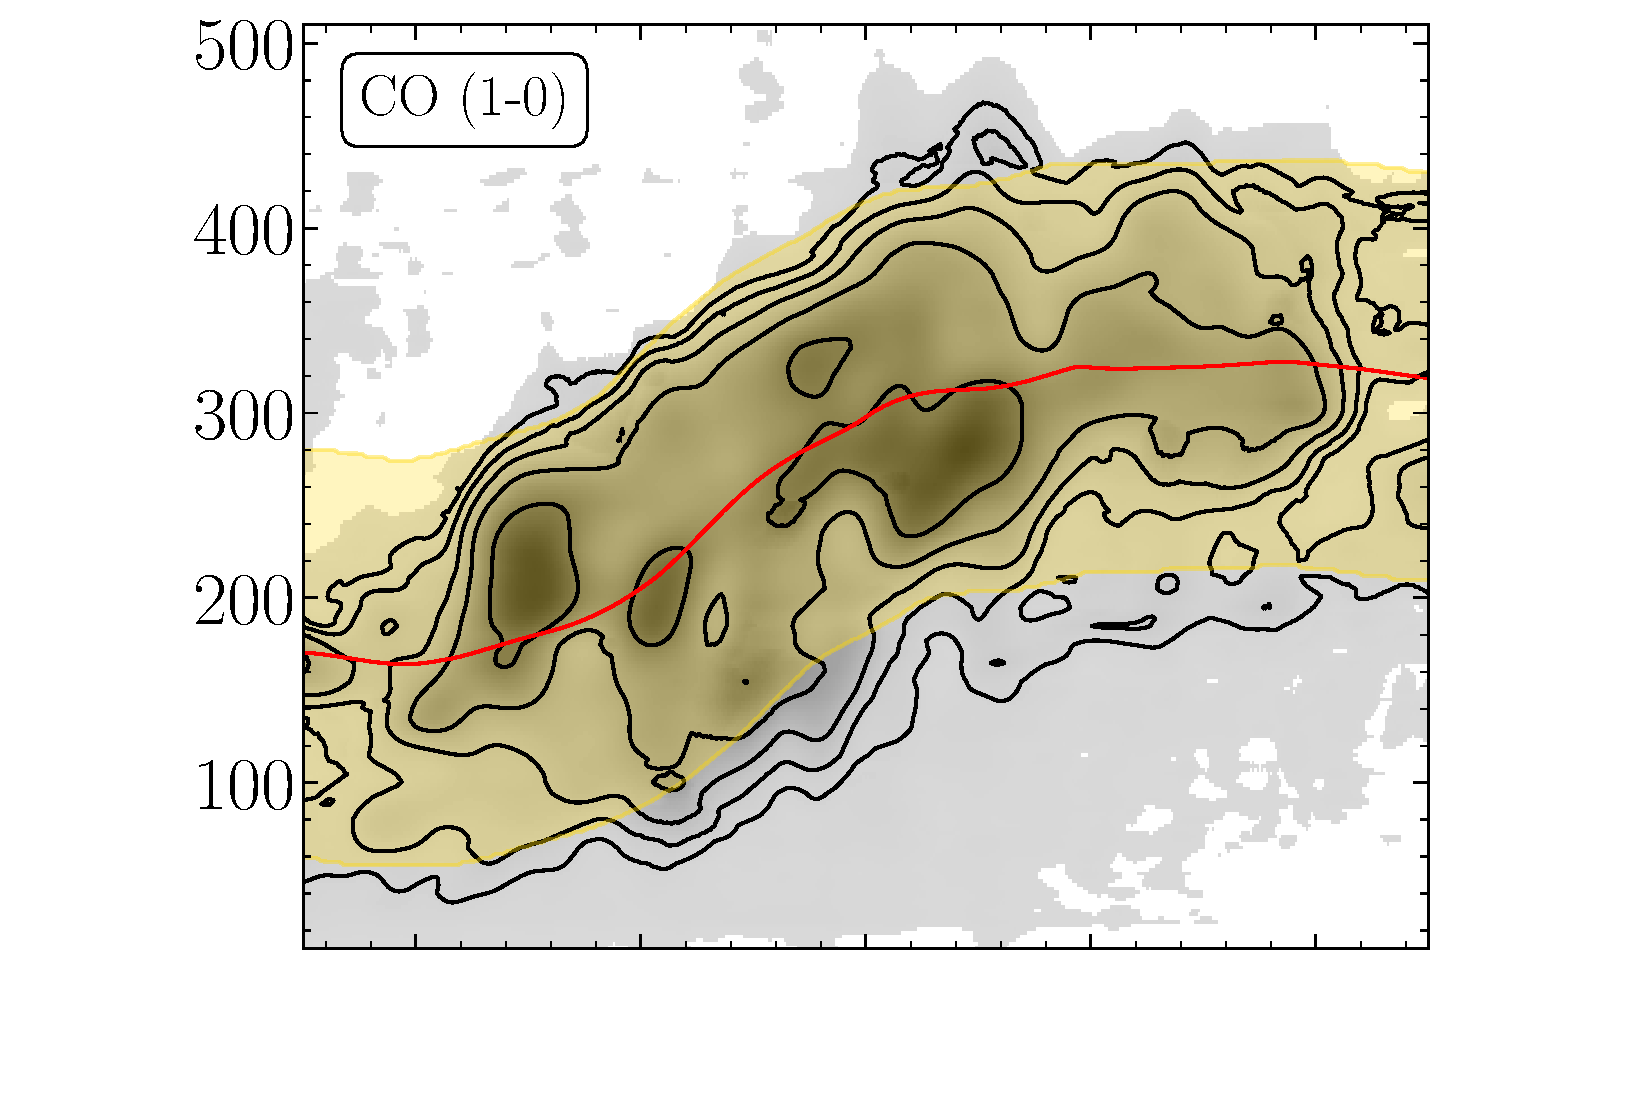
\includegraphics[width=0.6\textwidth]{images/chapters/papers/outflow/outflow_fig5a.pdf}
	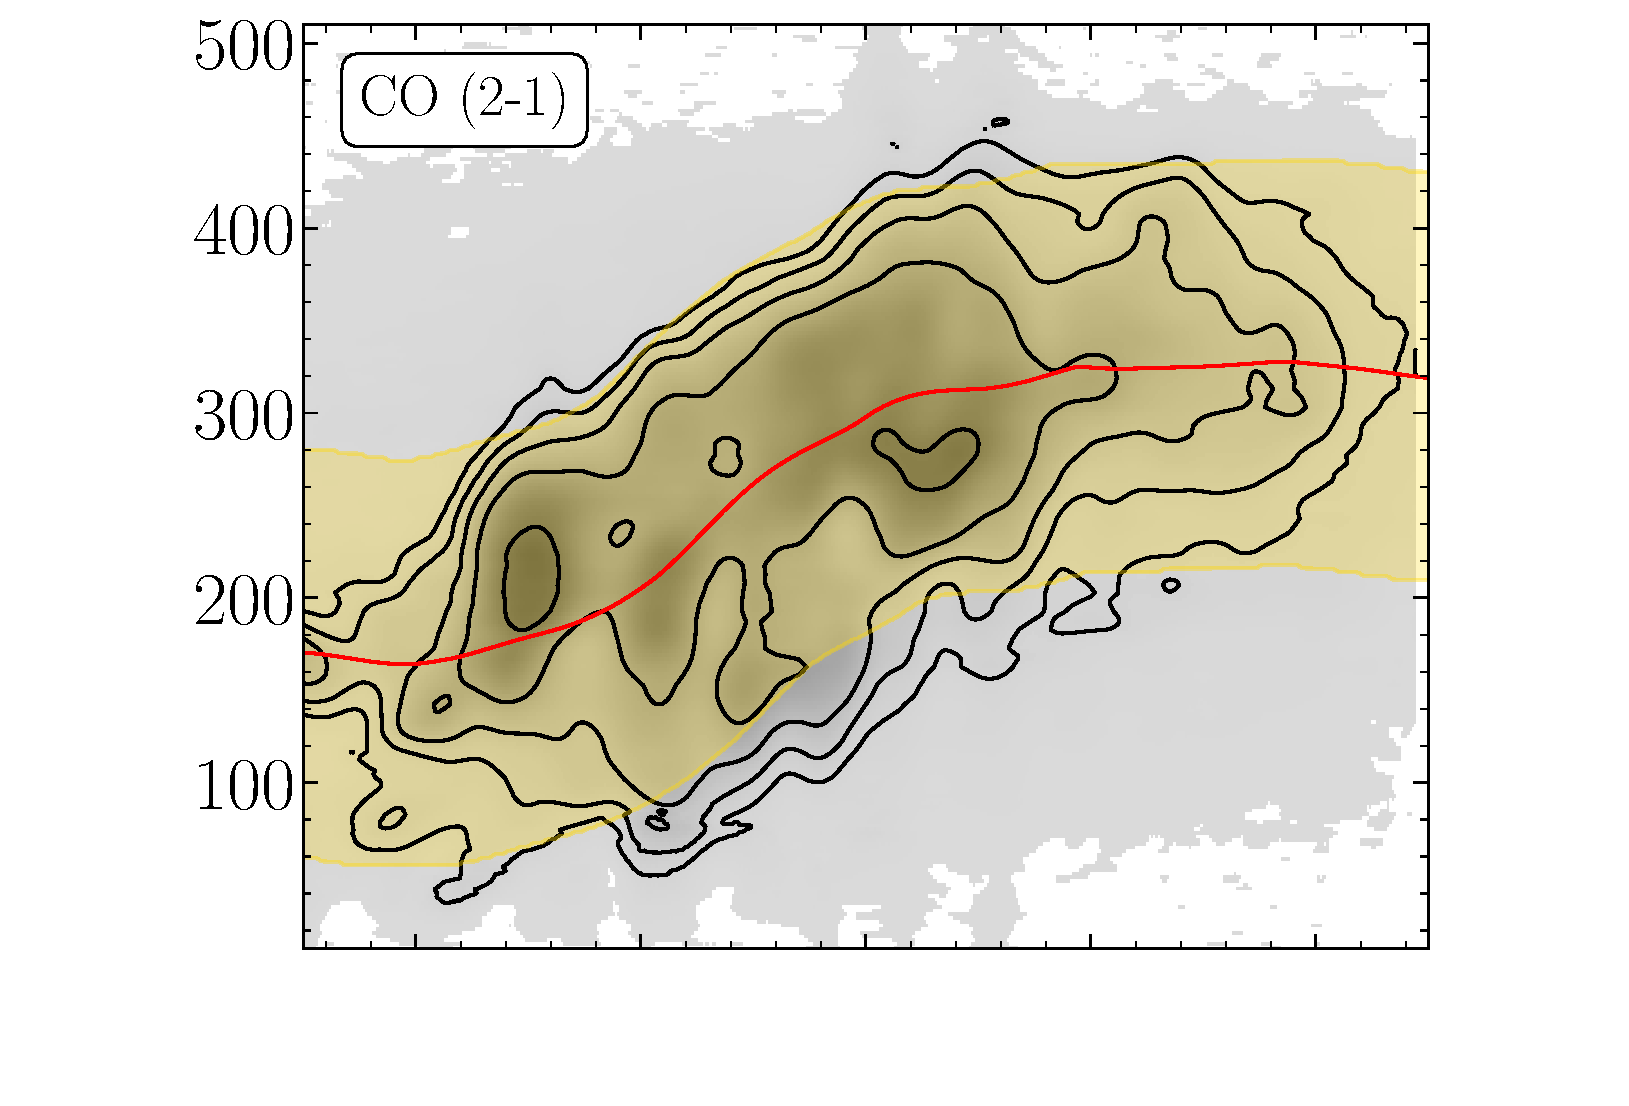
\includegraphics[width=0.6\textwidth]{images/chapters/papers/outflow/outflow_fig5b.pdf}
	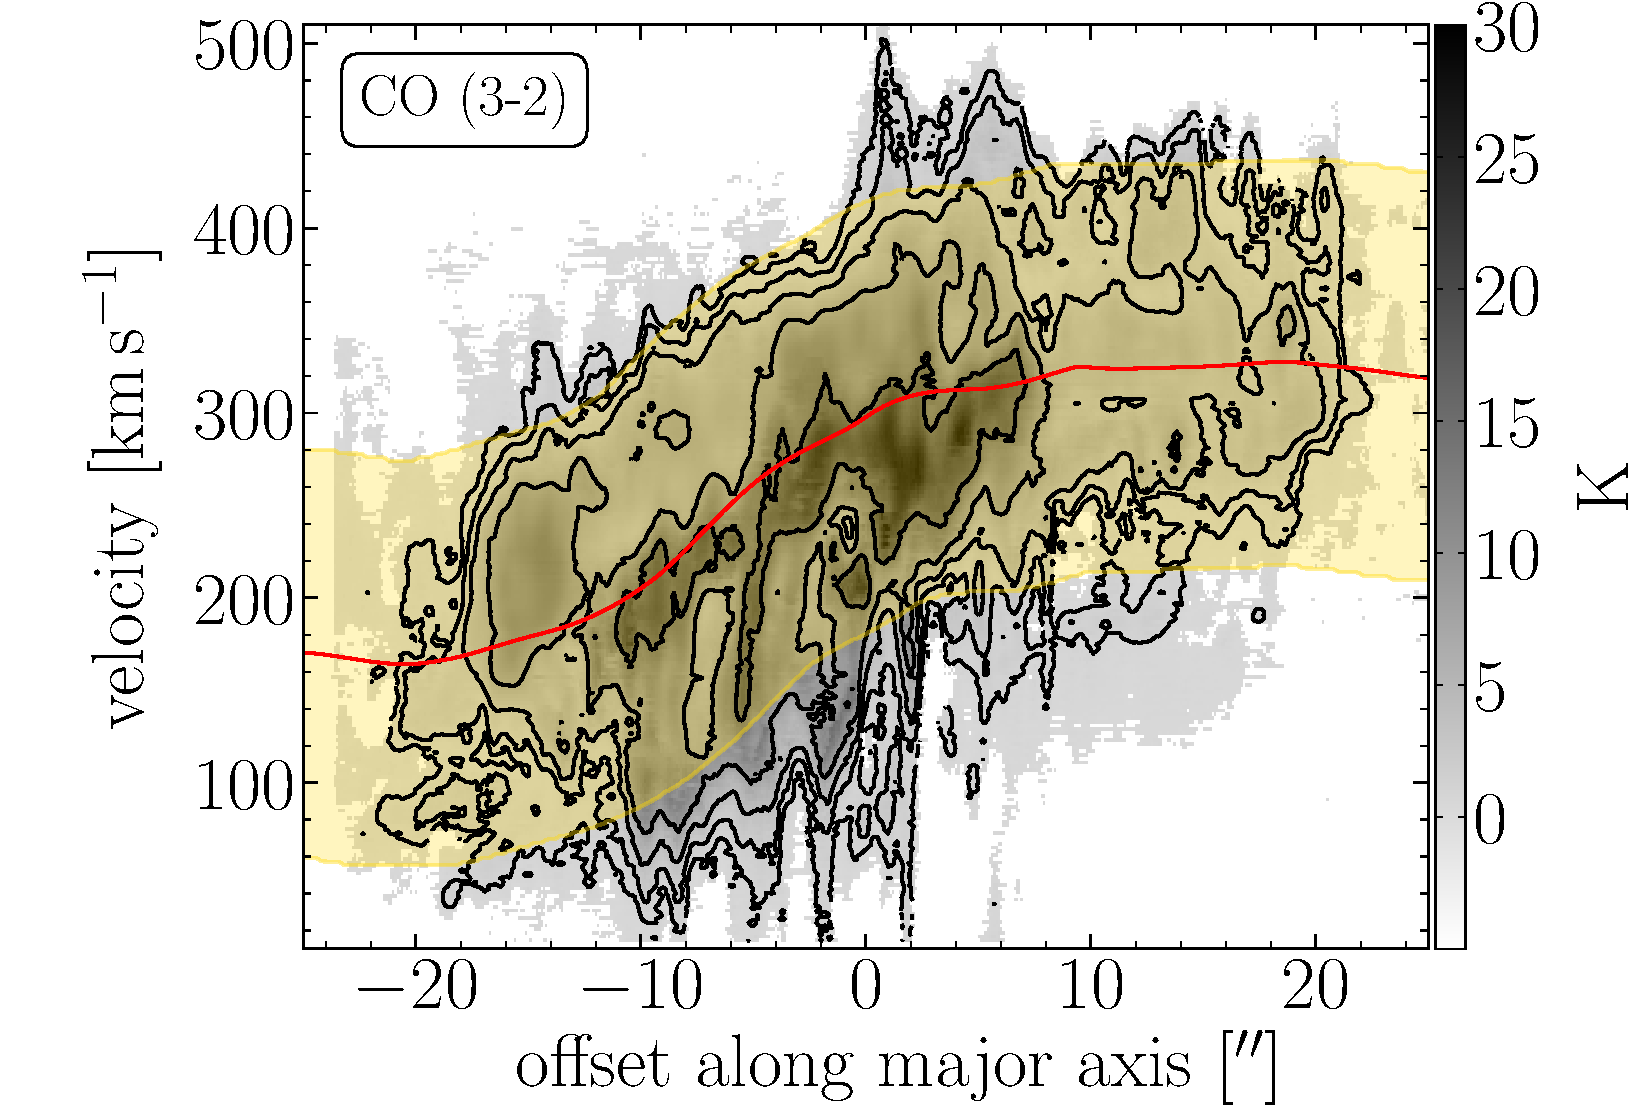
\includegraphics[width=0.6\textwidth]{images/chapters/papers/outflow/outflow_fig5c.pdf}
	\caption[Sample pV slices]{Position-velocity diagram of the central slice (offset $0.0\arcsec$) showing the construction of the disk/non-disk masks. The background images show the flux density above $5.0 \sigma$ for \co10 (top), \co21 (center) and \co32 (bottom) on identical gray scale. Contours are drawn at 1, 2, 4, 8 and 16\,K. The central velocity for our model of the disk emission is illustrated by the red line. The golden-shaded area denotes the disk mask. Similar figures for other offsets are shown in Appendix~\ref{appendix: outflow: all pVs}. Note that the different transitions have different angular resolution.}
	\label{outflow: figure: sample slice}
\end{figure}


%%%%%%%%%%%%%%%%%%%%%%%%%%%%%%%%%%%%%%%%%%%%%%%%%%%%%%%%%%%%%%%%%%%%%%%%%%%%%%%%%%%%%%%%%%%%%%%%%%%%

\subsection{Identifying  outflows in the non-disk component}

We identify three different types of structures in the non-disk component (Figure~\ref{outflow: figure: separated moments}, contours in Figure~\ref{outflow: figure: nondisk zoomin} highlight these structures): 

(1) Emission that is co-located with the central disk and bar in projection. This is visible as a ridge in \co32 (inner contour in Figure~\ref{outflow: figure: nondisk zoomin}), and also present but less apparent in \co10 and \co21. The structure is unlikely to be an outflow. It appears more likely to be an additional kinematic component of the disk/bar that is not included in the model we used for the separation. We therefore do not consider this gas to contribute to the total mass outflow rate. 

(2) Emission associated with the so-called western superbubble, located to the west and north of the central starburst region \citep[][shown by the western contour in Figure~\ref{outflow: figure: nondisk zoomin}]{2006ApJ...636..685S,2013Natur.499..450B}. This feature is already known to be kinematically distinct from the surrounding gas. Part of it is likely the base of the northern outflow cone (and giving rise to the NW streamers identified by \citeauthor{2013Natur.499..450B}, for example), but it is difficult to know what portion of the emission should be associated with a net outflow. 
In our calculations below we exclude this feature from the total outflow rate of \ngc253, although it likely has some contribution to outflow.

(3) The remaining gas associated with the non-disk component is organized in small clumps along the edge of the disk region or beyond it. Some of this gas is not discernible as individual structures, particularly in the \co10 and \co21 cubes, perhaps due to the resolution but maybe also due to the excitation conditions, constituting extended regions with diffuse emission. Some of the emission is located in well-defined structures known to be part of the outflow, such as the SW streamer which is apparent in all CO transitions.

In summary, the non-disk component consists of these three sub-components: structures that we associate with a net ``outflow,'' structures that are part of the ``western superbubble,'' and structures that are co-located with the ``disk''. The latter is not associated with the outflow, while parts of the western supperbubble may contribute to it. Below we calculate properties for the two components disk and non-disk, and its sub-components individually where it is feasible to do so.


%%%%%%%%%%%%%%%%%%%%%%%%%%%%%%%%%%%%%%%%%%%%%%%%%%%%%%%%%%%%%%%%%%%%%%%%%%%%%%%%%%%%%%%%%%%%%%%%%%%%
%%%%%%%%%%%%%%%%%%%%%%%%%%%%%%%%%%%%%%%%%%%%%%%%%%%%%%%%%%%%%%%%%%%%%%%%%%%%%%%%%%%%%%%%%%%%%%%%%%%%

\section{Results}
\label{outflow: section: results separated disk/non-disk}

The process described in the previous section allows us to estimate the properties of the galactic outflow and other structures. 
A 2D representation of the separated data cubes is shown in Figure~\ref{outflow: figure: separated moments} in the form of moment maps for integrated intensity (moment 0) and intensity-weighted velocity (moment 1) for all three CO transitions. Striping artifacts due to the pV cuts used in the separation method are present in the disk and non-disk components, visible as straight lines parallel to the major axis. This is primarily aesthetic. We tested their effects on the fluxes and derived velocities by varying the slice width and found them to be negligible.

\begin{figure*}
	\caption[Separated disk and non-disk CO emission]{Comparison between original moment maps and separated disk/non-disk components. The outline of the maps is defined by the observed field of view and the square region considered for separating the kinematic components.).
	}
	\subfloat[
	Moment 0 (integrated intensity) of the original image (\emph{top}), disk component (\emph{middle}) and non-disk component (\emph{bottom}). The logarithmic color scales are identical for all panels and chosen to also show the fainter non-disk component which saturates the inner regions of the disk. Contours are drawn at $\log \left( F\ \lbrack \mathrm{K\,km\,s}^{-1} \rbrack \right) = 1.7, 2.0, 2.3, 2.6, 2.9, 3.2, 3.5$; for clarity, only every other contour is drawn for \co32.
	]{
		\centering
		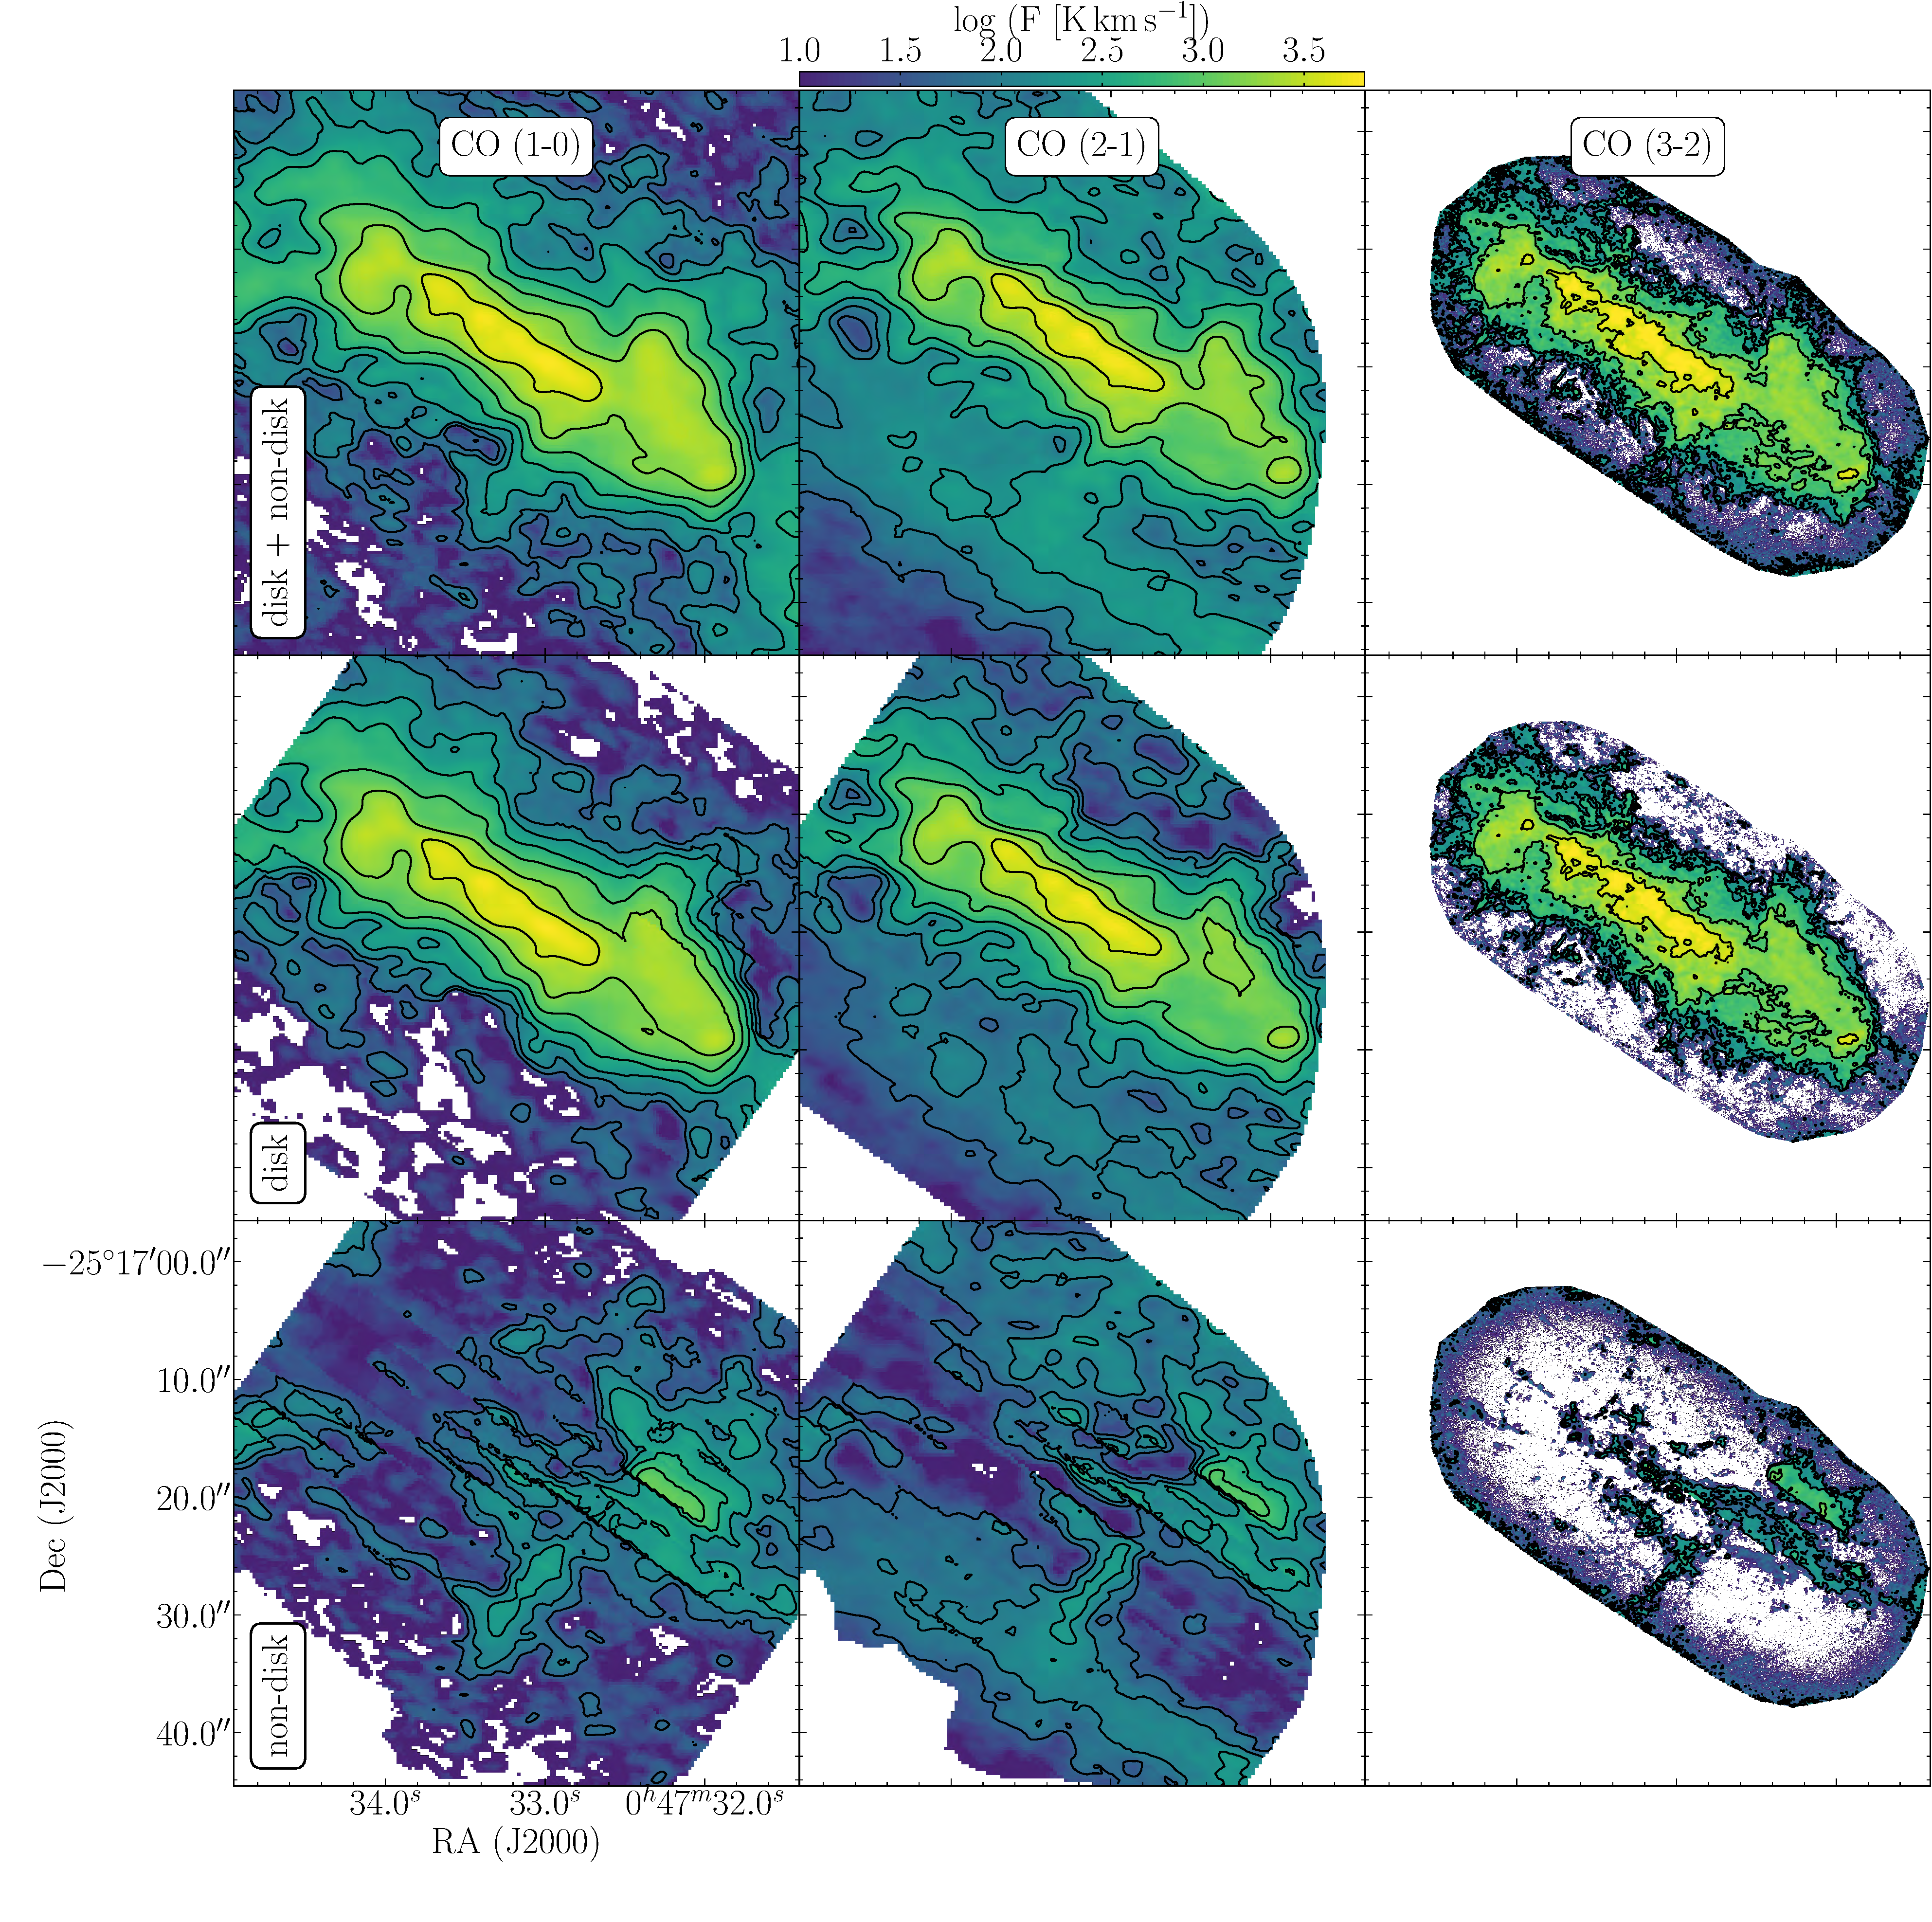
\includegraphics[width=\linewidth]{images/chapters/papers/outflow/outflow_fig6a.pdf}
	}
	\label{outflow: figure: separated moments}
\end{figure*}
\begin{figure*}
	\ContinuedFloat
	\centering
	\subfloat[
	Moment 1 (intensity-weighted velocity) of the original image (\emph{top}), disk component (\emph{middle}) and non-disk component (\emph{bottom}). Contours are drawn at 150, 200, ..., 350\,\kms. The noise edge visible in \co32 is due to primary beam correction required to derive accurate fluxes.
	]{
		\centering
		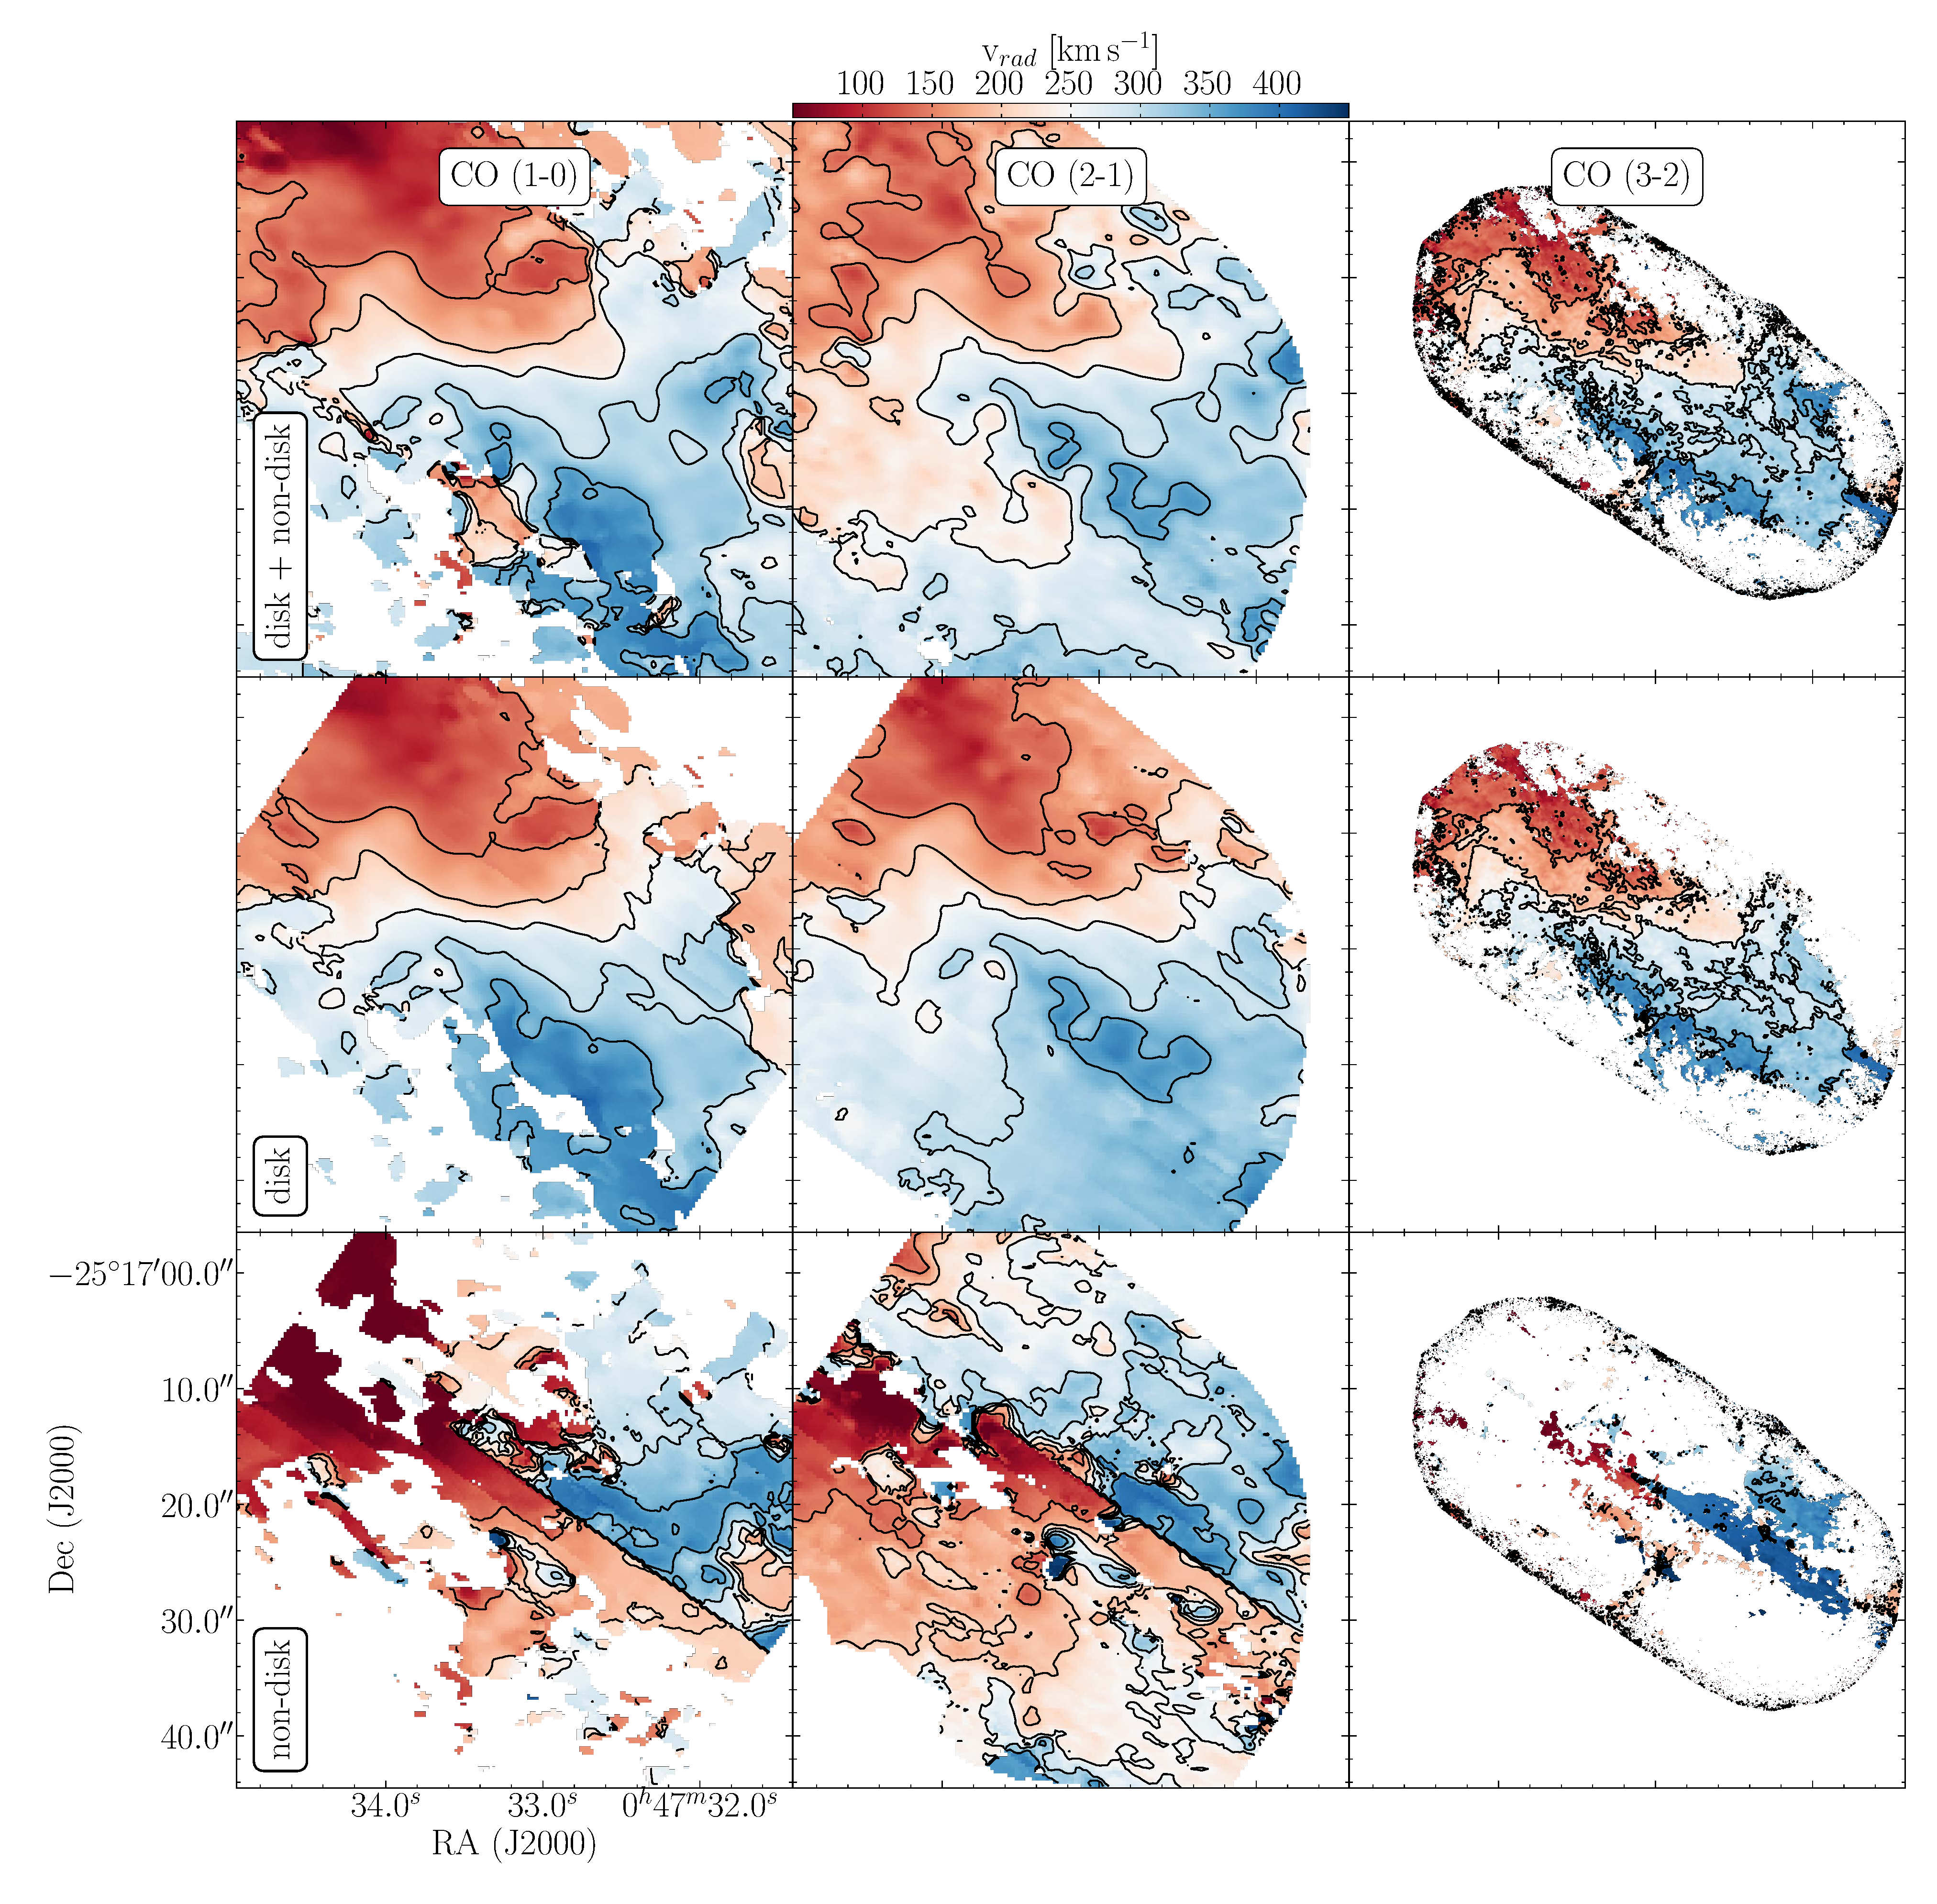
\includegraphics[width=\linewidth]{images/chapters/papers/outflow/outflow_fig6b.pdf}
	}
	% add one to figure counter to get correct figure numbers
	\stepcounter{figure}
\end{figure*}

\begin{figure}
    \centering
    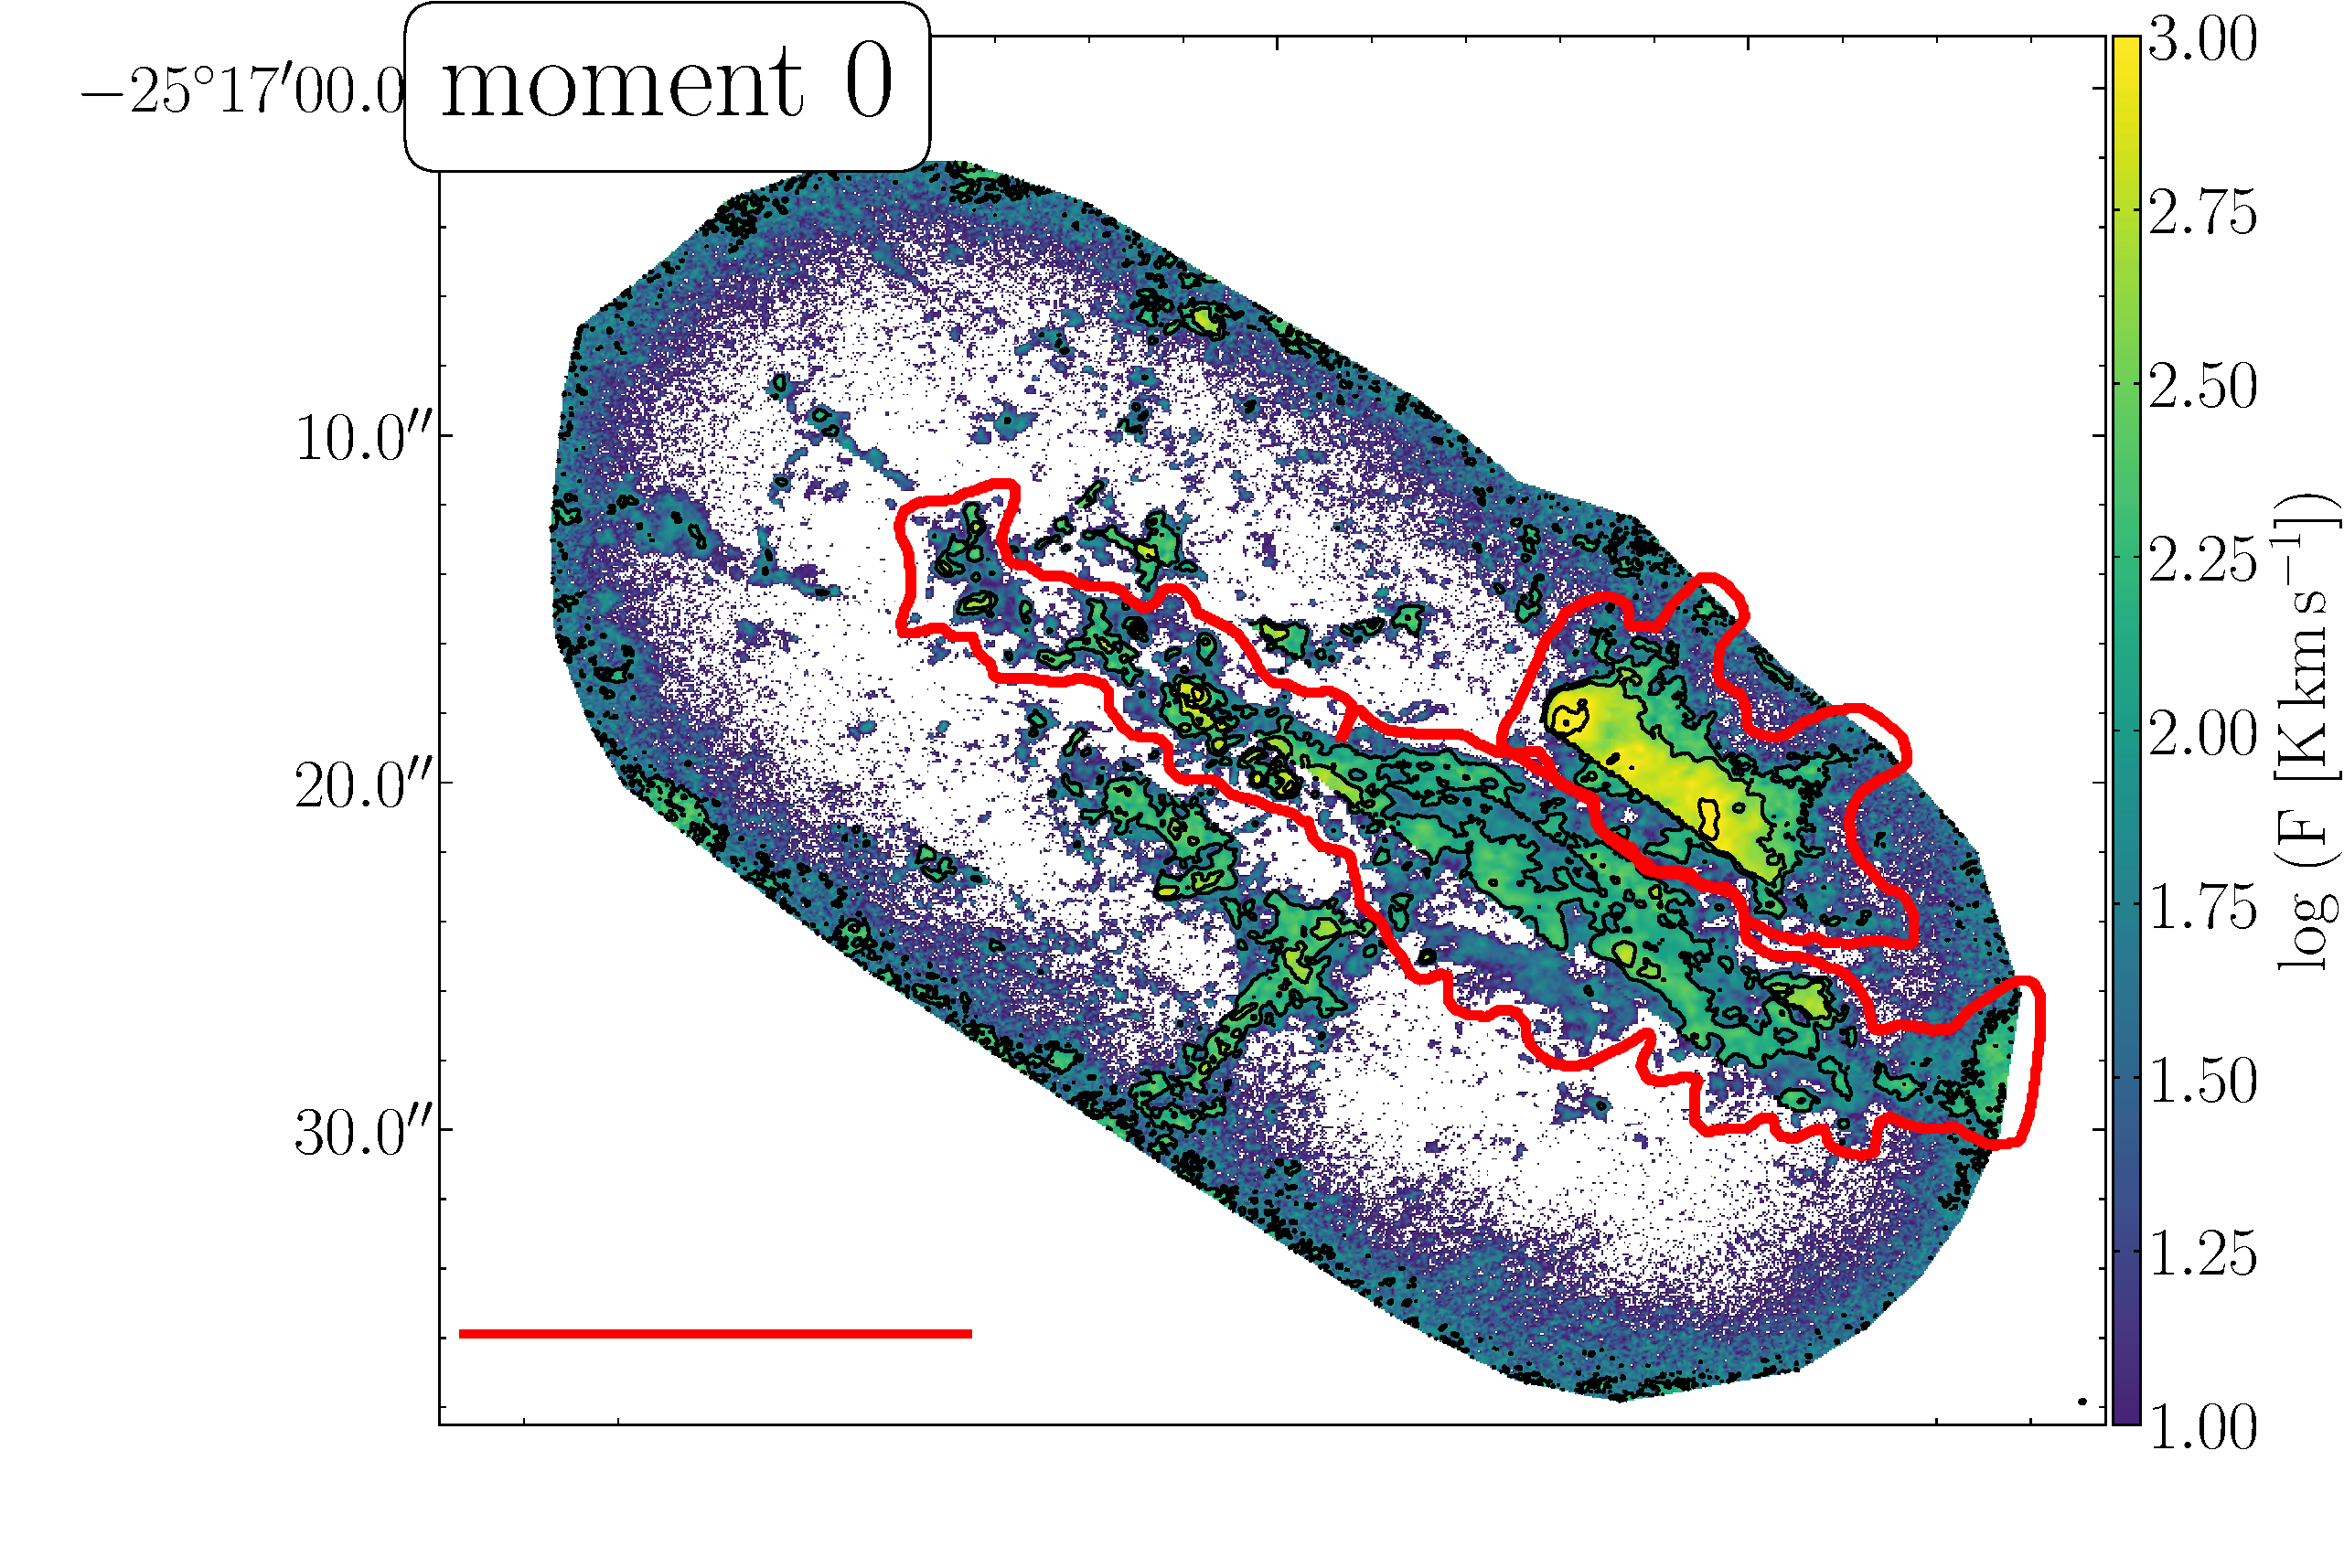
\includegraphics[width=0.6\linewidth]{images/chapters/papers/outflow/outflow_fig7a.pdf}\\
    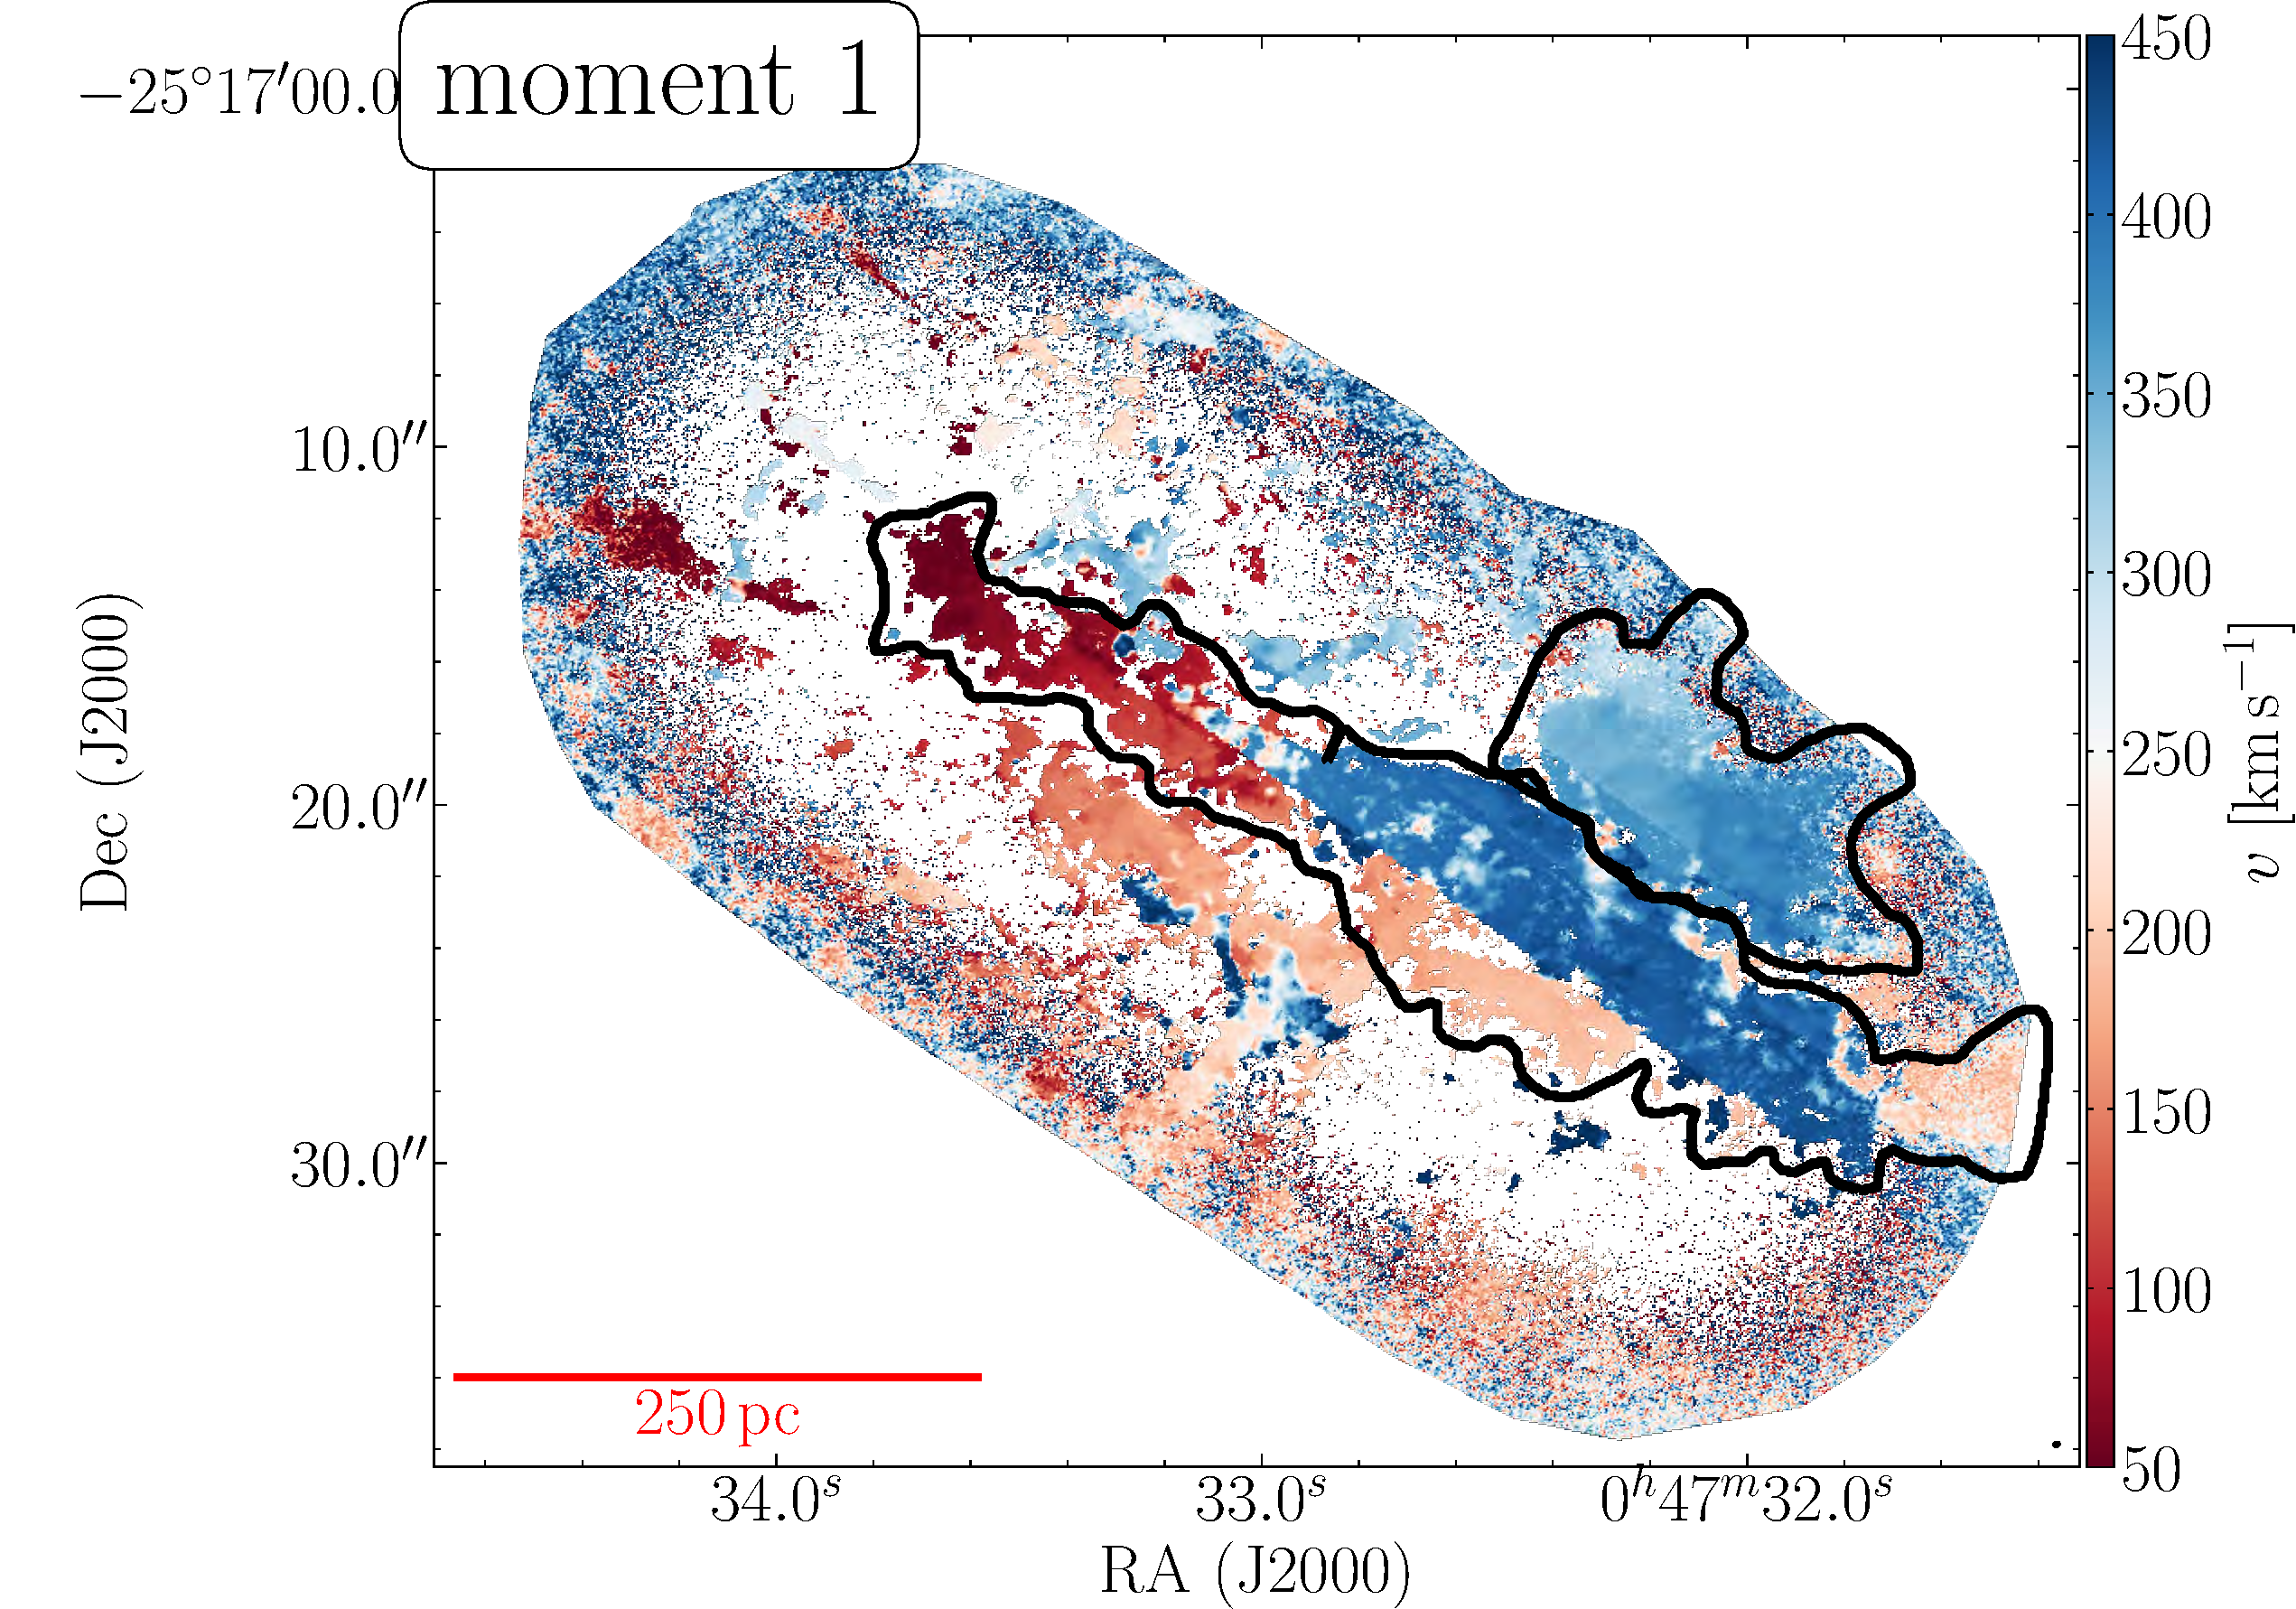
\includegraphics[width=0.6\linewidth]{images/chapters/papers/outflow/outflow_fig7b.pdf}
    \caption[Zoom-in on the non-disk \co32 of Figure~\ref{outflow: figure: separated moments}]{A zoom-in on the non-disk component of \co32 (the bottom left panels in Figure~\ref{outflow: figure: separated moments}a and \ref{outflow: figure: separated moments}b). \emph{Top}: Moment~0 (integrated intensity) with contours at $\log \left( F\ \lbrack \mathrm{km\,s}^{-1} \rbrack \right) = 2.0, 2.5, 3.0$. \emph{Bottom}: Moment~1 (intensity-weighted velocity). The thick contours show the regions discussed in the text (Section~\ref{outflow: section: outflow rate}): gas that is kinematically not consistent with disk rotation but co-spatial with the disk in projection, and the western superbubble to the north-west of the disk.}
    \label{outflow: figure: nondisk zoomin}
\end{figure}


%%%%%%%%%%%%%%%%%%%%%%%%%%%%%%%%%%%%%%%%%%%%%%%%%%%%%%%%%%%%%%%%%%%%%%%%%%%%%%%%%%%%%%%%%%%%%%%%%%%%

\begin{table}
    \centering
    \begin{threeparttable}
	    \caption[Results of separating disk from non-disk emission in \ngc253]{Results of separating disk from non-disk emission in \ngc253. Uncertainties for these quantities are discussed in the corresponding subsections of Section~\ref{outflow: section: results separated disk/non-disk}.
	    \label{outflow: table: results}}
	    \scriptsize
	    \begin{tabular}{lccccccc}
\toprule
quantity & unit & \multicolumn{2}{c}{\co10} & \multicolumn{2}{c}{\co21} & \multicolumn{2}{c}{\co32}\\
\cmidrule{3-4} \cmidrule{5-6} \cmidrule{7-8}
         &      & disk & non-disk           & disk & non-disk           & disk & non-disk\\
\midrule
\multicolumn{2}{l}{\textbf{luminosity}}\\
L$_\mathrm{CO}$ & \Kkmspc & $2.8 \times 10^8$ & $4.2 \times 10^7$ & $2.3 \times 10^8$ & $4.5 \times 10^7$ & $1.8 \times 10^8$ & $1.2 \times 10^7$ \\
fraction & \% & 87 & 13 & 84 & 16 & 94 & 6.5 \\
\midrule
\multicolumn{2}{l}{\textbf{molecular gas mass $\mathrm{M}_\mathrm{mol}$ \tnote{\dag}}}\\
total\tnote{a} & \Msun & $3.1 \times 10^8$ & $4.5 \times 10^7$ & $3.1 \times 10^8$ & $6.1 \times 10^7$ & $2.9 \times 10^8$ & $2.0 \times 10^7$ \\
\phantom{---}outflow\tnote{b} & \Msun & & $2.7 \times 10^7$ & & $4.1 \times 10^7$ & & $8.3 \times 10^6$ \\
\phantom{---}superbubble\tnote{c} & \Msun & & $8.9 \times 10^6$ & & $8.9 \times 10^6$ & & $5.8 \times 10^6$ \\
\phantom{---}other-disk\tnote{d} & \Msun & & $7.6 \times 10^6$ & & $7.4 \times 10^6$ & & $5.8 \times 10^6$ \\
\midrule
\multicolumn{2}{l}{\textbf{molecular mass outflow rate $\dot{M}$} \tnote{\ddag}}\\
\phantom{---}outflow (continuous)\tnote{e} & \Msunyr & & 14 & & 20 & & 2.7 \\
\phantom{---}outflow (constant)\tnote{f} & \Msunyr & & 29 & & 39 & & 4.8 \\
\midrule
\multicolumn{2}{l}{\textbf{kinetic energy $\mathrm{E}_\mathrm{kin}$ \tnote{\S}}}\\
\phantom{---}outflow (continuous)\tnote{e} & \ergs & & $3.9 \times 10^{54}$ & & $4.5 \times 10^{54}$ & & $6.5 \times 10^{53}$ \\
\phantom{---}outflow (constant)\tnote{f} & \ergs & & $2.5 \times 10^{54}$ & & $3.1 \times 10^{54}$ & & $4.3 \times 10^{53}$ \\
\midrule
\multicolumn{2}{l}{\textbf{momentum $\mathrm{P}$ \tnote{\P}}}\\
\phantom{---}outflow (continuous)\tnote{e} & \Msunkms & & $6.9 \times 10^8$ & & $8.7 \times 10^8$ & & $1.2 \times 10^8$ \\
\phantom{---}outflow (constant)\tnote{f} & \Msunkms & & $4.8 \times 10^8$ & & $6.4 \times 10^8$ & & $8.0 \times 10^7$ \\
\bottomrule
        \end{tabular}
        \begin{tablenotes}
\item[a] CO line luminosity of all emission considered consistent with disk rotation (disk) and not consistent with disk rotation (non-disk), respectively.
\item[b] Non-disk excluding the western superbubble and the gas that is co-spatial with the projected disk.
\item[c] Non-disk emission belonging to the western superbubble as defined by \citet{2006ApJ...636..685S}.
\item[d]Non-disk gas that is co-spatial with the disk in projection. See Section~\ref{outflow: section: outflow rate} for the definition.
\item[e] Outflowing gas as defined by note $^b$ under the assumption of continuous mass ejection without accelerations to the gas after ejection.
\item[f] Outflowing gas as defined by note $^b$ under the assumption of approximately constant starting mass outflow rate over the lifetime of the starburst.
\item[\dag] Molecular gas mass derived using a conversion factor for \co10 emission of $\mathrm{X}_{\mathrm{CO}} = 0.5\times10^{20}\,\left(\mathrm{K\,km\,s}^{-1}\right)^{-1}$, including the contribution of Helium, and assuming CO brightness temperature line ratios of $r_{21} = 0.80$ and $r_{31} = 0.67$ for \co21 and \co32 relative to \co10.
\item[\ddag] Deprojected molecular mass outflow rate. $50^{th}$ percentile best estimate assuming a flat distribution of outflow inclinations for the unknown geometry.
\item[\S] Deprojected kinetic energy of the molecular gas. $50^{th}$ percentile best estimate assuming a flat distribution of outflow inclinations for the unknown geometry.
\item[\P] Deprojected momentum of the molecular gas. $50^{th}$ percentile best estimate assuming a flat distribution of outflow inclinations for the unknown geometry.
\item Sources of error are discussed and quantified in the respective subsections of section \ref{outflow: section: results separated disk/non-disk}.
        \end{tablenotes}
    \end{threeparttable}
\end{table}


%%%%%%%%%%%%%%%%%%%%%%%%%%%%%%%%%%%%%%%%%%%%%%%%%%%%%%%%%%%%%%%%%%%%%%%%%%%%%%%%%%%%%%%%%%%%%%%%%%%%

\subsection{CO luminosities}

We quantify in Table~\ref{outflow: table: results} the CO luminosities of the disk and non-disk components. We measure luminosities of $2.8 \times 10^8$\,\Kkmspc, $2.3 \times 10^8$\,\Kkmspc and $1.8 \times 10^8$\,\Kkmspc for \co10, (2--1) and (3--2), respectively, in the central disk of \ngc253. The non-disk component is, naturally, much fainter with luminosities of $\sim 4.2 \times 10^7$\,\Kkmspc for \co10, $\sim 4.2 \times 10^7$\,\Kkmspc for (2--1) and $\sim 4.2 \times 10^7$\,\Kkmspc (3--2). These correspond to approximately $12.9\%$, 16.4\% and 6.5\% of the total luminosity. These luminosities are measured over the sliced area (cf.\ Figure~\ref{outflow: figure: slice positions}) for which the coverage is not the same among the datasets. We therefore also measure luminosities integrated over the same spatial region, here defined as the overlap between the datasets. This overlap amounts to 885\,\arcsec$^2$ ($2.55\times10^5$\,pc$^2$). The luminosities in the overlap area are: disk: $2.6 \times 10^8$\,\Kkmspc, $2.1 \times 10^8$\,\Kkmspc and $1.8 \times 10^8$\,\Kkmspc; non-disk: $2.6 \times 10^7$\,\Kkmspc, $2.4 \times 10^7$\,\Kkmspc and $1.2 \times 10^7$\,\Kkmspc for \co10, (2--1) and (3--2), respectively.

An interesting result coming out of our decomposition is that not all the material we identify as ``outflow'' is in well-defined structures such as the streamers identified by \citet{2013Natur.499..450B}. Correctly estimating the outflow rate requires accounting also for a diffuse extended component. 

It is important to compare our fluxes to measurements in the literature. \citet{1996A&A...305..421M} find a \co21 luminosity of $1.2 \times 10^6$\,K\,\kms\,arcsec$^2$ which translates\footnote{adjusting from the distance $\mathrm{D} = 2.5$\,Mpc used by \citeauthor{1996A&A...305..421M} to the $\mathrm{D} = 3.5$\,Mpc assumed here} to $3.5 \times 10^8$\,\Kkmspc or $1.3$ times our measurement. Their observations cover $80\arcsec \times 60\arcsec$,
a area similar to our \co10 observations (but $\sim 4$ times larger than the area of our \co32 observations). For the outflow \co10 luminosity, \citet{2013Natur.499..450B} derive an estimate of $2.0 \times 10^7$\,\Kkmspc by summing over individual identified molecular outflow features. This includes flux from the ``superbubble'' component, so it is probably better compared to the sum of our ``outflow'' and ``superbubble'' components of $\sim3.6\times10^7$\,\Kkmspc. Given the large methodological differences and the importance of the diffuse emission, these numbers are in reasonable agreement. 


%%%%%%%%%%%%%%%%%%%%%%%%%%%%%%%%%%%%%%%%%%%%%%%%%%%%%%%%%%%%%%%%%%%%%%%%%%%%%%%%%%%%%%%%%%%%%%%%%%%%

\subsection{Masses of components}
\label{outflow: section: mass distribution}

The total gas mass $M$ is estimated from the CO line luminosity, using the conversion factor $\mathrm{X}_{\mathrm{CO}} = 0.5\times10^{20}\,(\mathrm{K\,km\,s}^{-1})^{-1}$\,\sqcm corresponding to $\alpha_\mathrm{CO} = 1.1\,\mathrm{M}_\odot\,(\mathrm{K\,km\,s}^{-1}\,\mathrm{pc}^{-1})^{-1}$ discussed by \citet{Leroy:2015ds} for the central starburst region. This value accounts for the effects of moderate optical depth, high velocity dispersion, and warm gas temperatures that are likely to dominate the central regions of \ngc253. The masses we report include the contribution of Helium to the total mass. To compute masses using the \co21 and \co32 transitions we assume typical line ratios of $r_{21} = 0.80$ and $r_{31} = 0.67$ relative to \co10 as implied by \citet{2018ApJ...867..111Z}. Note that we do not measure line ratios from the images but adopt a uniform factor to keep the mass measurements from the three observed CO lines independent.

Table~\ref{outflow: table: results} lists the masses corresponding to the disk and the non-disk components. Uncertainty in the mass estimates arises primarily from the assumed conversion factor and the apportioning of emission among the different components. The calibration uncertainty for the flux measurements is $\sim10-15\%$ for the ALMA observations. Overall, we adopt a systematic error of factor $\sim2$ for the the derived masses.

The molecular masses derived from the three CO transitions are very similar. They match within 10\% for the disk component, and within 50\% for the non-disk component. We estimate the total gas mass in the center of \ngc253 to be $\sim 3.5 \times 10^8$\,M$_\odot$ (adding the disk and non-disk components), with estimates in the range of $3.1-3.6 \times 10^8$\,\Msun for the different transitions. About 85\% of the total mass is in the disk component. The masses estimated in the non-disk components using \co10 and \co21 are fairly similar at $4.5 \times 10^7$\,\Msun and $6.1 \times 10^7$\,\Msun whereas in \co32 we detect a lower $2.0 \times 10^7$\,\Msun, a consequence of the lower luminosity. The non-disk masses are primarily contributed by the outflow component ($\sim 50$\%). About $20-30$\% of mass is in the western supperbubble and $12-30$\% is co-spatial with the disk but kinematically distinct.

It is important to compare these mass estimates to previous results for the total molecular gas mass in \ngc253, noting that our analysis
covers the central $45\arcsec \times 25\arcsec$ ($750\,\mathrm{pc} \times 400\,\mathrm{pc}$). Towards the east, $\sim 10\%$ of the known molecular gas close to the center is not covered by our \co32 observations and thus not considered in this analysis. The agreement with previous measurements is very good. \citet{1996A&A...305..421M} reported a mass of $1.3 \times 10^8$\,\Msun over a similar area ($80\arcsec \times 60\arcsec$ in the center of \ngc253), but this was based on a different distance and $\mathrm{X}_{\mathrm{CO}}$. After correcting for those differences, their luminosity corresponds to $4.2 \times 10^8$\,\Msun, consistent with our measurement. Using the same distance and the same 1--0 observations, \citet{Leroy:2015ds} measure a molecular mass of $3.5 \times 10^8$\,\Msun. 
\citet{2018ApJ...860...23P} report a total gas mass of $4.5 \times 10^8$\,\Msun\ derived from the sub-mm dust spectral energy distribution, which is very consistent with our result given the very different methodologies. 

No estimates in the literature separate the ``disk'' and ``non-disk'' components as we do above. Previous estimates of the outflowing mass range from a lower limit of $6.6 \times 10^6$\,\Msun calculated for the optically thin limit \citep{2013Natur.499..450B}, to $2-4 \times 10^7$\,\Msun  when accounting for optical depth \citep{2018ApJ...867..111Z}. Since we identify an outflowing mass $\sim5\times10^7$\,\Msun, the agreement with the latter estimate is fairly good. Note, however, that these studies derive the outflowing mass from individual features rather than using the position-velocity information as we do here in a systematic way.


%%%%%%%%%%%%%%%%%%%%%%%%%%%%%%%%%%%%%%%%%%%%%%%%%%%%%%%%%%%%%%%%%%%%%%%%%%%%%%%%%%%%%%%%%%%%%%%%%%%%

\subsection{Mass outflow rate}
\label{outflow: section: outflow rate}

\begin{figure}
    \centering
    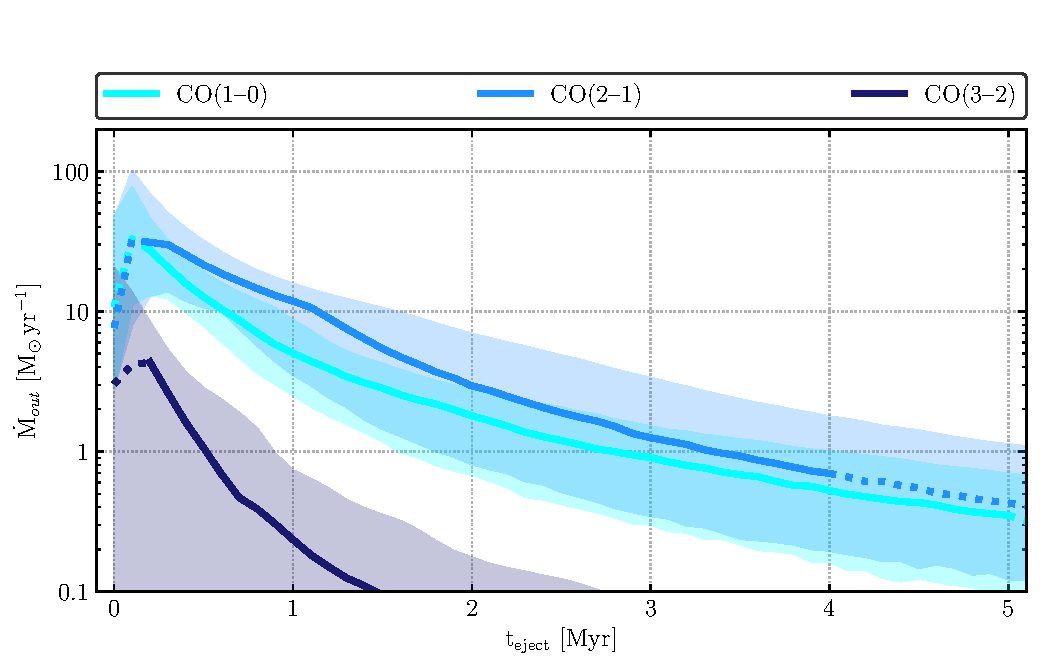
\includegraphics[width=0.8\linewidth]{images/chapters/papers/outflow/outflow_fig8a.pdf}
    \\ \vspace{0.2cm}
    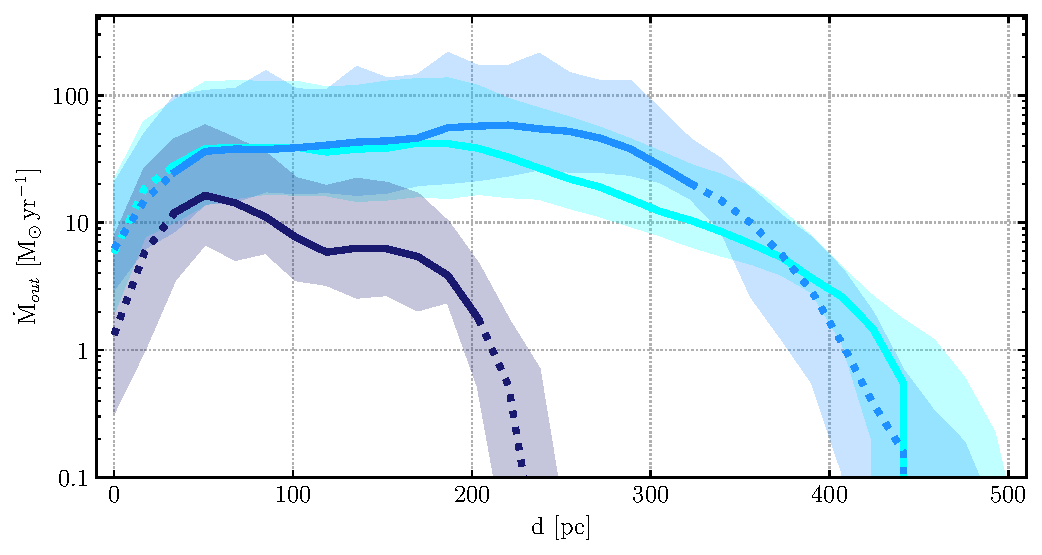
\includegraphics[width=0.8\linewidth]{images/chapters/papers/outflow/outflow_fig8b.pdf}
    \caption[Molecular mass outflow rate]{Deprojected molecular mass outflow rate averaged over 0.1\,Myr as a function of time since ejection (\emph{top}) and as a function of deprojected distance between outflow and launching site (\emph{bottom}). The top panel implicitly assumes continuous mass ejection without accelerations to the gas after ejection,  while the lower panel assumes approximately constant starting mass outflow rate over the lifetime of the starburst. The shaded area indicates approximate errors ($16^{th}$ to $84^{th}$ percentile), which are dominated by uncertainties in the deprojection geometry. Dotted lines represent the ranges where confusion with gas in the disk occurs and where the limited field-of-view affects the completeness.}
    \label{outflow: figure: outflow rate}
\end{figure}

A mass flow rate is defined as the flux of mass per unit time through a surface. In our case, we are interested in the flow of molecular gas mass through a virtual closed surface around the center of \ngc253 at a given distance. Note that an individual outflow feature observed over a certain length, such as the SW streamer, can develop in at least two ways: as the distance of an outflow from its origin corresponds to time since ejection times velocity, continuously outflowing gas results in extended streaming structures. Gas ejected at a single ejection event in the past with a distribution of ejection velocities, on the other hand, will also result in an extended streamer. In reality gas will be ejected with a distribution of velocities at a varying rate over a period of time, and in order to interpret the measurements we need to make some simplifying assumptions. We chose two edge cases to span the range of different interpretations: (1) the gas does not experience accelerations after being launched \citep[however, see ][]{2017ApJ...835..265W}, and (2) that the gas outflow rate is approximately constant with time. For all calculations, however, we assume that the projected direction of flow is perpendicular the the central plane of the bar and that CO emission traces the mass with a constant conversion factor.

We compute both the outflow rate as a function of distance and as a function of time. If we assume that the mass outflow rate has been approximately constant over the lifetime of the starburst, for example, a diminishing outflow rate as a function of distance would suggest that gas is either launched with or somehow develops a distribution of velocities. Conversely, if we assume that the present day velocity has been constant since the gas was ejected, we can derive a history of the mass outflow rate as a function of time and account for a variable mass outflow rate. Both interpretations are equally, but not simultaneously, valid.

For the detailed calculation of the mass outflow rate, we proceed as follows. A mass outflow rate is $\dot{\mathrm{M}} = \mathrm{M} \,t^{-1}$ with mass M and relevant time scale $t$. For each image element $i$ (3D pixel or sometimes also called voxel), we calculate the outflow rate $\dot{m}_i$ of the gas that was ejected at time $t_{{\mathrm{eject}},i}$ over the time interval $\Delta t_{\mathrm{cross},i}$, as the ratio of mass of the pixel ${m}_i$ to the pixel crossing interval $t_{\mathrm{cross},i}$. Ejection time and pixel crossing interval are functions of the outflow velocity $v_i$ and the distance $s_i$ between current pixel position and the launching site, and the pixel size in the direction of the flow $\Delta s$, respectively. We therefore compute
\begin{equation}
    \Delta t_{\mathrm{cross},i}   = \frac{\Delta s}{v_i}\\    
    \dot{m}_i\ (t_{\mathrm{eject},i}) = \frac{m_i}{\Delta t_{\mathrm{cross},i}}\\
    t_{\mathrm{eject},i} = \frac{s_i}{v_i}
\end{equation}

\noindent obtaining a mass outflow rate $\dot{m}_i$, a distance $s_i$, and an ejection time $t_{\mathrm{eject},i}$ for each pixel in the ``outflow'' component. Note that this approach takes the 3D phase space information into account by treating pixels independently. Typically, a sightline shows multiple pixels with emission at different velocities that all contribute an outflow rate with their respective mass, distance and velocity. We then bin the outflow rates $\dot{m}_i$ by ejection time $t_{\mathrm{eject},i}$ and integrate over the time range $\left[\mathrm{T}_1, \mathrm{T}_2 \right]$ to obtain the average outflow rate in this time interval,
\begin{equation}
    \dot{M} \left( \mathrm{T}_1, \mathrm{T}_2 \right) = 
    \frac{\displaystyle \sum_i \dot{m}_i \left( \mathrm{T}_1 \LESS t_{\mathrm{eject},i} \LESS \mathrm{T}_2 \right)  \Delta t_{\mathrm{cross},i} }{\displaystyle \mathrm{T}_2 - \mathrm{T}_1 }.
    \label{equation: outflow rate time}
\end{equation}

\noindent Similarly, binning by distance results in the average outflow rate at a given distance, 
\begin{equation}
    \dot{M} \left( \mathrm{D}_1, \mathrm{D}_2 \right) =
    \frac{\displaystyle \sum_i \dot{m}_i \left( \mathrm{D}_1 \LESS s_i \LESS \mathrm{D}_2 \right) \Delta s }{\displaystyle \mathrm{D}_2 - \mathrm{D}_1 }.
    \label{equation: outflow rate distance}
\end{equation}
\noindent Performing binning on a sequence of time intervals yields the outflow rate history, while binning in distance tells us how far from the launching site a given fraction of the mass is able to escape.

Calculating velocity $v$ and distance $s$ requires knowledge about the geometry and origin of each outflowing gas parcel. The simplest assumption, used here, is that on average outflows are launched in the plane of the central region of the galaxy which corresponds to launching on the major axis. The distance $s$ is thus the projected distance to the major axis on the edge of an outflow cone with given opening angle. Note that the outflow originates from an extended region in the disk and the term cone thus refers to a cut-off cone (called a frustum in geometry). Velocity $v$ is the velocity difference between launching site and current velocity of the outflow parcel, i.e. the velocity difference over distance $s$. Both the velocity of the launching site and the projected distance are uncertain. The velocity changes by $\pm 25$\,\kms when an outflow originates from the northern/southern edge of the observed CO disk (above/below the plane), while the projected distance traveled by the gas changes by $\pm1.25\arcsec$ ($\pm20$\,pc).

Distance $s$, ejection time scale $t_\mathrm{eject}$ and pixel crossing time scale $t_\mathrm{cross}$ are measured as projected quantities that need to be deprojected to account for the outflow geometry. The bright molecular streamers (the SW and SE streamers) seem to lie at the edge of the ionized outflow cone with $\sim60^\circ$ opening angle \citep{2013Natur.499..450B}. Assuming that all molecular outflows are along this cone, and that the axis of the cone is oriented perpendicular to the disk ($i = 78^\circ$), the range of effective inclination of outflowing gas can be anywhere between $\theta = 48^\circ$ and $\theta = 108^\circ$. Deprojected velocity, $v_\mathrm{depro} = v_\mathrm{obs} / \sin\theta$, and distance, $s_\mathrm{depro} = s_\mathrm{obs} / \cos\theta$, have a direct effect on the deprojected outflow rate, $\dot{m}_\mathrm{depro} = \dot{m}_\mathrm{obs} \tan\theta$, and also on the inferred time and distance evolution of the outflow rate. We use a Monte Carlo approach to derive the errors introduced by deprojection, assuming that the outflow direction has an equal probability of being in any direction along the surface of the outflow cone.

Figure~\ref{outflow: figure: outflow rate} shows the molecular mass outflow rate as a function of time or distance, corresponding to the two alternative interpretations we discuss above: a flow where the distribution of material is interpreted as resulting from the history of mass outflow rate (top panel), and one where we show the mass outflow rate as a function of distance, which under the assumption of a constant outflow rate over the last several Myr can be interpreted as an efficiency of ejection to a given distance (bottom panel). Indeed, for an outflow with a distribution of velocities the slower material will not travel as far in a given time, neither will it escape the galaxy if it does not have a high enough velocity. 
Close to the starburst region (or at small times since ejection) the mass outflow rate drops to zero, because it becomes increasingly difficult to separate the ``outflow'' component from the ``disk'' component. At large values of distance or time it also drops to zero, due to a decreasing amount of outflowing molecular material detected far from the starbursts (and the fact that the observations have a limited field-of-view).
The constant outflow rate out to $\sim 300$\,pc is in tension with \citet{2018ApJ...853..173K} who find a steeply dropping ``cold'' ($\mathrm{T} \LESS 5050$\,K) component in their TIGRESS simulation. Within 400\,pc, they find the averaged mass loading factor to drop by two orders of magnitude. It is unlikely that the SFR in \ngc253 has increased by two orders of magnitude within the past 1-2\,Gyr which would alter the observed constant outflow rate profile to be consistent with the \citet{2018ApJ...853..173K} simulation. Note, however, that their simulation recreates solar neighborhood-like conditions instead of a starburst. A direct comparison may thus be not possible.

Our data show that the \emph{average} outflow rates within 20\arcsec (340\,pc) from the major axis are 29\,\Msunyr ($^{+0.48}_{-0.35}$\,dex), 39\,\Msunyr ($^{+0.49}_{-0.34}$\,dex) and 4.8\,\Msunyr ($^{+0.50}_{-0.39}$\,dex) for \co10, (2--1) and (3--2) respectively. Similarly, within the past 1.0\,Myr, the \emph{average} outflow rates are 14\,\Msunyr ($^{+0.25}_{-0.29}$\,dex), 20\,\Msunyr ($^{+0.27}_{-0.37}$\,dex) and 2.7\,\Msunyr ($^{+0.22}_{-0.56}$\,dex) for \co10, (2--1) and (3--2) respectively. The uncertainties, indicated by the $16^{th}$ to $84^{th}$ percentile in the Monte Carlo described above, are substantial at a factor of $2-3$. Real systematic uncertainties are even larger, since there can be conversion of molecular into atomic material \citep[c.f. ][]{2015ApJ...814...83L}, or in general variations in the CO-to-H$_2$ conversion.

Note that the average outflow rates quoted above differ between the two representations, with the median outflow rate as a function of distance being about twice as high as a function of time. The outflowing mass is identical in both cases, and the difference arises solely from binning. Comparing between lines, it is apparent that as measured in \co32 the outflow rate is roughly one order of magnitude lower than for the lower two transitions. This is a direct consequence of the lower mass detected in \co32, and the smaller field-of-view of those observations. The \co32 observations cover only $\sim 12.5\arcsec$ ($\sim 210$\,pc projected) above/below the disk and thus miss significant amounts of non-disk gas. Their lower surface brightness sensitivity means we also fail to detect a diffuse non-disk component, as we see in the two lower lines. The measurements in \co32 should thus be interpreted as a lower limit, and in that sense they are consistent with those for the lower two transitions.

Overall, the deprojected total mass outflow rate in the starburst of \ngc253 is most likely in the range $\sim 14-39$\,\Msunyr as derived from \co10 and \co21 with $\sim 0.4$\,dex uncertainty. The large spread arises due to different interpretations of the kinematics of the observed gas while the errors are due to unknown geometry.
The majority of this outflow rate is contributed by massive outflows alongside the disk like the SW/SE streamers, with a significant contribution by diffuse molecular gas.

The present day star formation rate in the central region of \ngc253 is  $1.7-2.8$\,\Msunyr, derived from radio continuum and far-infrared measurements \citep{Ott:2005il,Leroy:2015ds,2015MNRAS.450L..80B}. This results in a mass loading factor $\eta = \dot{M}_\mathrm{out} / \dot{M}_\mathrm{SFR}$ in the range $\eta \sim 5.4-23.5$. Note that this is for gas ejected as far as 340\,pc. We do not currently know what fraction of the gas makes it to the far regions of the halo, or reaches escape velocity from the system. Theoretical works suggest that most of the molecular outflow will not escape but rain back down on the galaxy (e.g. \citealt{Shapiro:1976ha} up to recent work by \citealt{2018ApJ...853..173K} or \citealt{2019MNRAS.tmp..540T}).

In our data, no gas reaches the escape velocity of $v_\mathrm{esc} = 500$\,\kms \citep{2017ApJ...835..265W}. The uncertainty on $v_\mathrm{esc}$ is substantial, so allowing a factor of two is still plausible. At $v_\mathrm{esc} = 250$\,\kms, the fraction of gas above $v_\mathrm{esc}$ by mass is 0.5\%, 0.5\% and 6.0\% for \co10, \co21 and \co32, respectively. The mismatch between the lower transitions and \co32 implies that some high velocity gas can be found on small scales that is blurred out in the low resolution observations.

This estimate of the molecular mass outflow rate is higher than the lower limit found by \citet{2013Natur.499..450B} for optically thin emission. \citet{2018ApJ...867..111Z} analysis of the CO line ratios in the SW streamer shows that the emission there is optically thick, which the authors used this to rescale the \citet{2013Natur.499..450B} measurements finding a \ngc253 galactic outflow rate of $25-50$\,\Msunyr. The result presented here, a mass outflow rate of $\sim 14-39$\,\Msunyr, is consistent with this number using an independent and a more complete methodology than the original work.

From H$\alpha$ observations by \citet{Westmoquette:2011bp}, we can estimate the ionized outflow rate to $\sim 4$\,\Msunyr using their ionized mass ($\mathrm{M} = 10^7$\,\Msun) and typical velocity (200\,\kms) at mean deprojected distance (510\,pc). X-ray observations yield comparable values. \citet{Strickland:2000wd} finds an upper limit of 2.2\,\Msunyr assuming a standard outflow velocity of 3000\,\kms. The upper limit reported in \citet{Strickland:2002kp} translates to 2.3\,\Msunyr when assuming 3000\,\kms outflow velocity and a reasonable 10\% filling factor. These estimates scale linearly with the unknown velocity and also depend on the unknown metallicity and filling factor in the outflow. Estimates of the outflow rate in neutral gas are not known in the literature but are arguably at a similar level.
The molecular phase thus clearly dominates the mass budget in the outflow close to the disk as found in other galaxies (e.g. M82, \citealt{2015ApJ...814...83L} and simulations, e.g. \citealt{2018ApJ...853..173K}).


%%%%%%%%%%%%%%%%%%%%%%%%%%%%%%%%%%%%%%%%%%%%%%%%%%%%%%%%%%%%%%%%%%%%%%%%%%%%%%%%%%%%%%%%%%%%%%%%%%%%

\subsection{Outflow energy and momentum}
\label{outflow: section: outflow energy}

% \begin{figure}
\begin{sidewaysfigure}
    \centering
    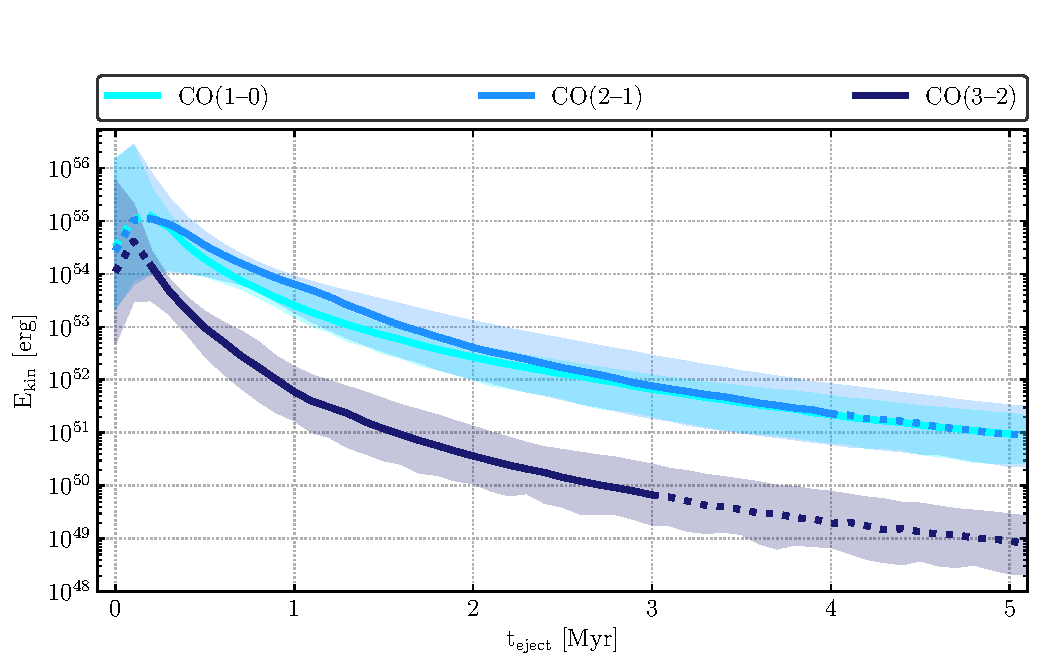
\includegraphics[width=0.48\linewidth]{images/chapters/papers/outflow/outflow_fig9a.pdf}~~
    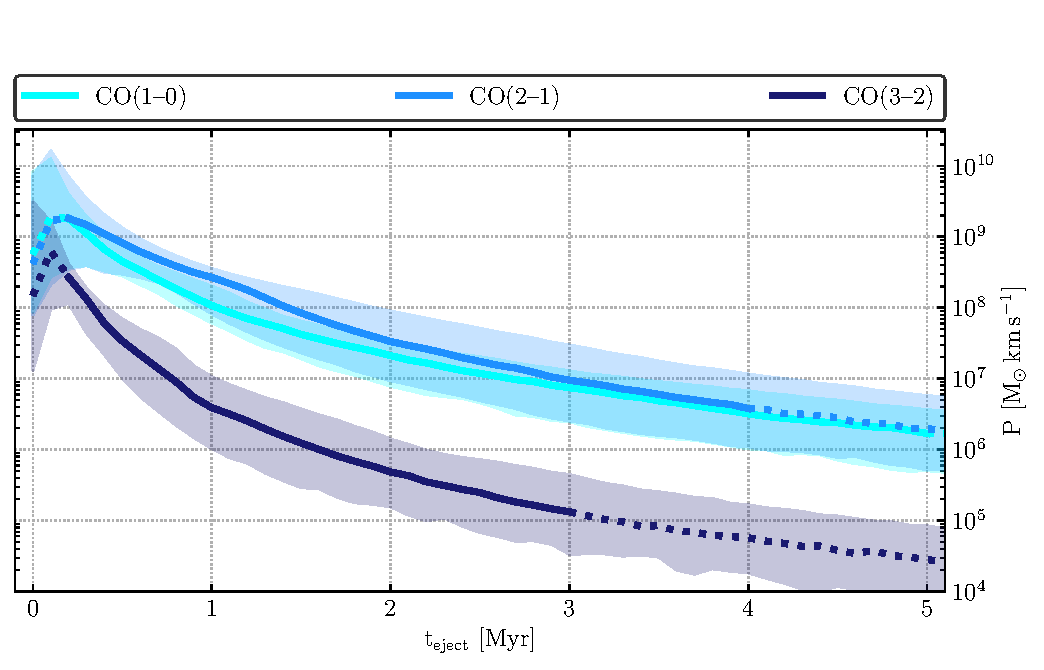
\includegraphics[width=0.48\linewidth]{images/chapters/papers/outflow/outflow_fig9b.pdf}
    \\
    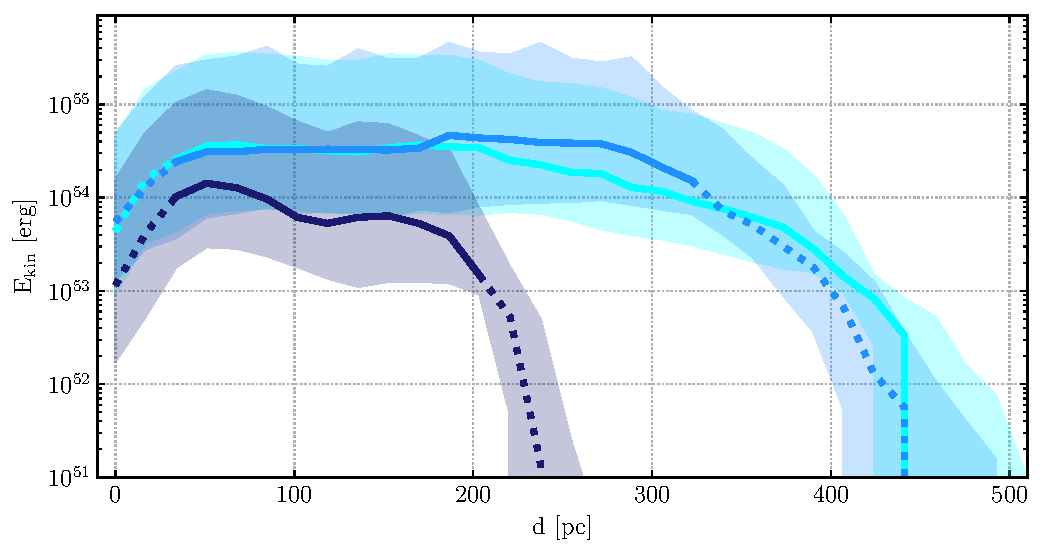
\includegraphics[width=0.48\linewidth]{images/chapters/papers/outflow/outflow_fig9c.pdf}~~
    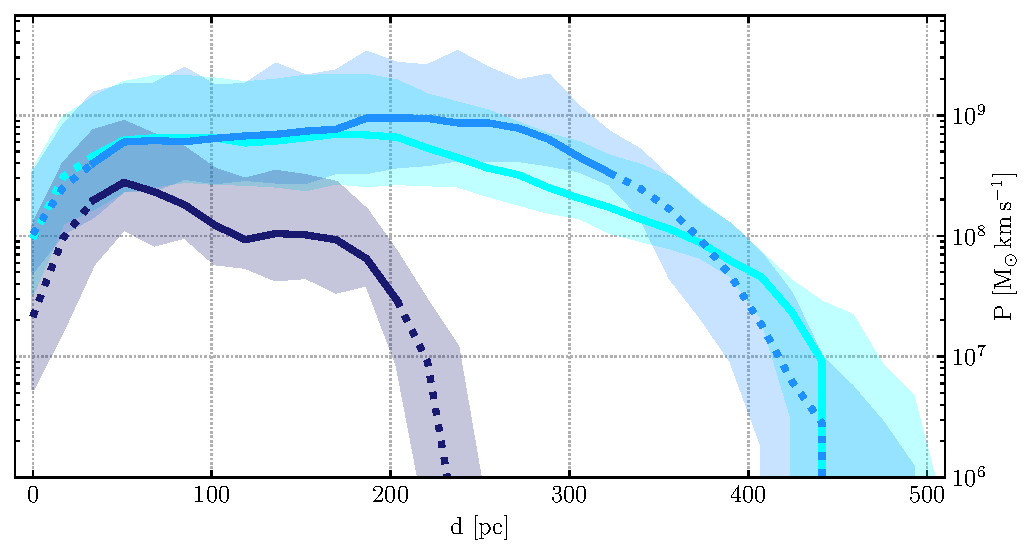
\includegraphics[width=0.48\linewidth]{images/chapters/papers/outflow/outflow_fig9d.pdf}
    \caption[Kinetic energy and momentum]{Deprojected kinetic energy (\emph{left}) and deprojected momentum (\emph{right}) of the molecular outflow averaged over 0.1\,Myr as a function of time since ejection (\emph{top}) and as a function of deprojected distance between outflow and launching site (\emph{bottom}). The top panel implicitly assumes continuous mass ejection without accelerations to the gas after ejection,  while the lower panel assumes approximately constant starting mass outflow rate over the lifetime of the starburst. The shaded area indicates approximate errors ($16^{th}$ to $84^{th}$ percentile), which are dominated by uncertainties in the deprojection geometry. Dotted lines represent the ranges where confusion with gas in the disk occurs and where the limited field-of-view affects the completeness.}
    \label{outflow: figure: outflow energy momentum}
\end{sidewaysfigure}
% \end{figure}

Similar to mass outflow rate, energy and momentum can be calculated as a function of time and distance which is shown in Figure~\ref{outflow: figure: outflow energy momentum}. In equations~\ref{equation: outflow rate time} and \ref{equation: outflow rate distance} the molecular outflow rate $\dot{m}_i$ is replaced by kinetic energy $E_{\mathrm{kin},i} = \frac{1}{2} m_i\,v_i^2$ or momentum $P_i = m_i\,v_i$. As with the outflow rate, the dominant sources of error are the uncertainty in the launching site and the geometry for which we Monte Carlo the errors as described before. Our median estimate with 16$^{th}$ and 84$^{th}$ percentile uncertainties are given below and in Table~\ref{outflow: table: results}.

The kinetic energy in the outflow integrated over the past 1.0\,Myr is $3.9 \times 10^{54}$\,erg ($^{+0.91}_{-0.75}$\,dex) in \co10, $4.5 \times 10^{54}$\,erg ($^{+0.94}_{-0.80}$\,dex) in \co21, and $6.5 \times 10^{53}$\,erg ($^{+0.58}_{-0.83}$\,dex) for \co32. Within 20\arcsec\ (340\,pc), the kinetic energies amount to $2.5 \times 10^{54}$\,erg ($^{+0.96}_{-0.65}$\,dex) in \co10, $3.1 \times 10^{54}$\,erg ($^{+0.96}_{-0.65}$\,dex) in \co21, and $4.3 \times 10^{53}$\,erg ($^{+0.98}_{-0.64}$\,dex) for \co32. For the reasons described above, the \co32 measurement is a lower limit, thus the results for the lower transitions are  consistent.

\ngc253 does not appear to host an energetically important AGN, and the outflow is driven by the starburst. It is interesting then to compare our results for the kinetic energy to the energy released by the starburst. We assume the current star formation rate of $\sim 2.8$\,\Msunyr in the central region \citep{Ott:2005il,2015MNRAS.450L..80B} that has been approximately constant over the last few Myr.

The total energy $E_\mathrm{bol}$ produced by the starburst is simply the time integrated bolometric luminosity $L_\mathrm{bol}$ which depends\footnote{We follow IAU resolution B2 that defines the bolometric magnitude in absolute terms and eliminates the dependence on the variable magnitude of the sun.} on the bolometric magnitude $M_\mathrm{bol}$.
\begin{align}
    E_\mathrm{bol} &= L_\mathrm{bol} \times \Delta t\\
    &= 3 \times 10^{35-0.4\,M_\mathrm{bol}} \Delta t \left( \frac{SFR}{1\,\mathrm{M}_\odot\,\mathrm{yr}^{-1}} \right)\,\mathrm{erg\,s}^{-1}
    \label{equation: bolometric energy}
\end{align}
According to Starburst99 \citep[figure~46 in][]{Leitherer:1999jt}, the bolometric magnitude of a starburst at an age of $10^7$\,yr to $10^8$\,yr is $M_\mathrm{bol} \sim -20.5$ for $\mathrm{SFR} = 1$\,\Msunyr.
The total energy output of the starburst over the past 1\,Myr is thus $4.2 \times 10^{57}$\,erg. The observed kinetic energy $\sim3.9-4.5\times10^{54}$\,erg in the outflow is a factor of $\sim 10^3$ lower which places the coupling efficiency of outflow kinetic energy to starburst energy at $\sim 0.1$\%.

In terms of only kinetic energy, the fraction is higher. Primarily supernovae and winds supply kinetic energy to the ISM which can be estimated from the energy deposition rate according to \citet{Leitherer:1999jt} as given in \citet{Chisholm:2017bu} and \citet{Murray:2005jt}.
\begin{equation}
    \dot{E}_\mathrm{SN} = 3 \times 10^{41} \left( \frac{SFR}{1\,\mathrm{M}_\odot\,\mathrm{yr}^{-1}} \right) \,\mathrm{erg\,s}^{-1}
    \label{equation: supernova energy}
\end{equation}
Each SN releases approximately $10^{51}$\,erg in kinetic energy, with the progenitor releasing a similar amount of kinetic energy during its lifetime by winds \citep[e.g.][]{Leitherer:1999jt}. The approximate total kinetic energy released by SNe in the past 1\,Myr is then $\sim 5.3 \times 10^{55}$\,erg, compared to the $\sim3.9-4.5\times10^{54}$\,erg we observe in the outflow. Hence, the observed starburst is sufficient to kinetically power the measured molecular outflows with $\sim 8\%$ efficiency.

The commonly adopted 50\% relative contribution of wind feedback is a first order estimate that is subject to environmental dependence and requires careful modeling to determine precisely \citep[e.g.][]{Leitherer:1999jt}. Furthermore, it should be noted that the observed outflow energy and its error is based on a fixed mass conversion factor that may vary. The uncertainty on the energy coupling efficiency is thus substantial and it should be understood as an order of magnitude comparison.

The above calculation ignores the contribution of other energies, such as the turbulent energy within the molecular outflow and the kinetic energy of the neutral and ionized gas. \citet{2009ApJ...701.1636M} derived a kinetic energy of the ionized wind in \ngc253 of $1.3 \times 10^{53}$\,erg or more than one order of magnitude lower than the molecular outflow kinetic energy. The molecular outflow is slower ($50-100$\,\kms on the scales we observed here) than the ionized outflow \citep[up to $\sim 400$\,\kms,][]{2009ApJ...701.1636M} but also more massive. The ionized outflow thus has only a very small effect on the total kinetic energy and the coupling efficiency.

Deprojected outflow momenta integrated over the past 1.0\,Myr are $6.9 \times 10^8$\,\Msunkms ($^{+0.50}_{-0.49}$\,dex), $8.7 \times 10^8$\,\Msunkms ($^{+0.57}_{-0.57}$\,dex) and $1.2 \times 10^8$\,\Msunkms ($^{+0.33}_{-0.59}$\,dex) for \co10, (2--1) and (3--2), respectively. Within 20\arcsec\ (340\,pc) deprojected distance from the launching site the outflow momenta integrate to $4.8 \times 10^8$\,\Msunkms ($^{+0.48}_{-0.35}$\,dex) in \co10, $6.4 \times 10^8$\,\Msunkms ($^{+0.49}_{-0.34}$\,dex) in \co21 and $8.0 \times 10^7$\,\Msunkms ($^{+0.50}_{-0.39}$\,dex) in \co32.

The momentum released initially by SNe is given in \citep{Murray:2005jt}:
\begin{align}
    \dot{P}_\mathrm{SN} &= 2 \times 10^{33} \left( \frac{SFR}{1\,\mathrm{M}_\odot\,\mathrm{yr}^{-1}} \right) \,\mathrm{g\,cm\,s}^{-2} \\
    &= 317 \left( \frac{SFR}{1\,\mathrm{M}_\odot\,\mathrm{yr}^{-1}} \right) \,\mathrm{M_\odot\,yr}^{-1}\,\mathrm{km\,s}^{-1}
    \label{equation: supernova momentum}
\end{align}
In 1\,Myr, a constant SFR of 2.8\,\Msunyr yields $8.9 \times 10^8$\,\Msunkms. Assuming a contribution by stellar winds of the same order \citep{Leitherer:1999jt}, the total momentum is $1.8 \times 10^9$\,\Msunkms or roughly twice the observed outflow momentum.
SNe, however, gain significant amounts\footnote{Assuming a Salpeter-like IMF ($\alpha=2.35$, mass range $0.1-100$\,\Msun, $\mathrm{Z} = 0.008$). The usual uncertainties related to the shape, upper mass cutoff and influence of binary stars apply.} of momentum by sweeping up surrounding material. From simulations, the total momentum supplied to the ISM is expected to be $2.8 \times 10^5$\,\Msunkms per SNe (\citealt{Kim:2015iy} and references therein). For a constant SFR of 2.8\,\Msunyr over 1\,Myr, this amounts to $1.0 \times 10^{10}$\,\Msunkms or $2.0 \times 10^{10}$\,\Msunkms when adopting 50\% contribution by stellar winds which is about four times the observed momentum. 
The efficiency of transferring feedback momentum to outflow momentum is thus in the range $27-49$\% considering the initially available momentum or $2.5-4$\% efficiency for total to outflow momentum transfer.

These outflow momenta are much higher than the momentum currently produced by young ($\LESS 10$\,Myr) super star clusters in the starburst. \citet{2018ApJ...869..126L} list 14 candidate clusters that together produce $1.5\times10^7$\,\Msunkms measured from gas kinematics, a factor $10-100$ lower than the observed outflow momentum. The currently forming (super-) star cluster thus could not have launched the outflow but the feedback of another population of stars is needed to explain the observed outflows. This is indicative of the time delay of SF feedback.

Energy and momentum curves in Figure~\ref{outflow: figure: outflow energy momentum} differ only by a factor $v$ but follow a similar evolution. This implies that the median velocity at a given distance must be roughly constant along the outflow. As the curves as a function of distance are roughly constant within $50\,\mathrm{pc} \LESS s \LESS 300\,\mathrm{pc}$, especially for kinetic energy, the outflow mass at a given distance must also be approximately constant along the outflow.
The decline in energy and momentum below 50\,pc is caused by a decrease in outflow mass, again because both curves follow a similar trend. This is at least partially related to the difficulty of separating outflow from disk where the former emerges from the latter. The decrease could also be interpreted physically as the outflow sweeping up mass while emerging from the disk. An estimation of the relative importance of these effects requires high-resolution modelling of the outflow that are not possible yet because we do not know the detailed outflow geometry.
The drop beyond $\sim 300$\,pc ($\sim 200$\,pc in \co32) is partially related to reaching the edge of the field-of-view. Discerning this effect from an actual decrease is not possible with our data as we do not know the inclination at every location in the outflow. The edge of the field-of-view thus corresponds to a range of deprojected distances from the disk which gradually depresses the curve rather than showing a sudden drop. A physical reason for the decrease could be the destruction of the molecular gas, e.g. photo-dissociation by the intense starburst radiation or ionization.

The kinetic energy and momentum evolution in Figure~\ref{outflow: figure: outflow energy momentum} thus suggest both energy and momentum conservation along the outflow from $\sim50$\,pc to $\sim 300$\,pc, as well as approximately constant molecular gas mass.

When additionally assuming no acceleration of the outflow after launch, it becomes possible to study the time evolution. The corresponding plots (Figure~\ref{outflow: figure: outflow rate} top and \ref{outflow: figure: outflow energy momentum} top) all show a peak within the past 0.5\,Myr and steady decrease towards earlier gas ejection times. Corresponding to the decline towards zero distance, the decrease towards zero ejection time is most likely a methodological complication. From the peak at t$_\mathrm{eject} = 0.2-0.3$\,Myr, kinetic energy and momentum in the outflow drops by a factor of 10 within $\sim 2$\,Myr. This decline would be physically plausible if the starburst in \ngc253 is very young and taking into account a time delay between start of star formation, feedback and efficient outflow driving (superbubble breakout). For the observed age of the starburst of $20-30$\,Myr \citep{Rieke:1980hh,Engelbracht:1998cj} this scenario is implausible. Time delays of $\GTR 20$\,Myr are longer than the lifetime of the most massive stars. A younger generation of massive stars at an age of $\sim 6$\,Myr \citep{Kornei:2009ee} may, however, drive the currently visible molecular outflows. If this were to be true, a time delay between star formation and outflow launching of $\sim 4$\,Myr is implied. Outflow launching in this context means the time after which the outflow reaches a mass loading $\eta \GTR 1$.
The time delay is 2\,Myr until the outflow carries more energy (momentum) than the feedback kinetic energy (momentum) of a single high mass star. Note that these rough estimates depend on the assumption of no acceleration (positive, nor negative) of the outflow after being launched from the disk which might be a close enough approximation on these scales of a few hundred parsecs.
The very young ($\LESSSIM 1$\,Myr) and still deeply embedded super star cluster discussed recently by \citet{2017ApJ...849...81A} and \citet{2018ApJ...869..126L} are most likely too young to have affected the observed molecular outflow.


%%%%%%%%%%%%%%%%%%%%%%%%%%%%%%%%%%%%%%%%%%%%%%%%%%%%%%%%%%%%%%%%%%%%%%%%%%%%%%%%%%%%%%%%%%%%%%%%%%%%

\section{Summary and Conclusions}
\label{outflow: section: summary}

We present \co32 observations taken with ALMA that offer an unprecedented resolution of $\sim 0.15\arcsec$ ($\sim 2$\,pc) in the starbursting center of \ngc253.
The new high resolution data show structures consistent with previous lower resolution observations in other CO lines,  revealing the complexity of the molecular ISM in a starburst on scales of a few parsecs. 

We use archival \co10, \co21, and the new \co32 ALMA observations to perform a position-position-velocity decomposition of the emission into different structures. The bulk of the emission is associated with a rotating disk with streaming motions due to the bar. The rest of the emission is incompatible with a simple kinematic model of a disk plus a bar. This ``non-disk'' component is further decomposed into an outflow, an expanding superbubble (part of which may be associated with outflowing gas) and a potential second kinematic component within the disk.

We find CO line luminosities of the disk component of $2.8\times10^8$\,\Kkmspc,\linebreak[4] $2.3\times10^8$\,\Kkmspc and $1.8\times10^8$\,\Kkmspc for \co10, (2--1) and (3--2), respectively. The fractional luminosity of the non-disk component is small, amounting the $\sim7-16\%$ of the total.  A significant amount of the outflow emission we identify is faint and diffuse, while part of the emission is in discrete, higher surface brightness structures (e.g., the SW streamer).

Assuming a starburst conversion factor, we estimate the molecular gas mass from the three CO transitions. Masses match within 10\% for the disk component and within 50\% for the non-disk component. The total gas mass in the center of \ngc253 is $\sim 3.6 \times 10^8$\,M$_\odot$, with $\sim 0.5 \times 10^8$\,M$_\odot$ in the non-disk component.

We further estimate the deprojected molecular mass outflow rate, kinetic energy and momentum in the starburst of \ngc253. The observed gas distribution can be interpreted to have formed in two ways: (1) by constant starting mass outflow rate over the lifetime of the starburst and (2) through continuous gas ejection without acceleration of the gas after ejection. In the first interpretation, the molecular mass outflow rate averaged over a deprojected distance of 340\,pc (20\arcsec) from the launching site is $29-39$\,\Msunyr. Typical uncertainties are 0.4\,dex. The majority of this outflow rate is contributed by massive localized features such as the SW/SE streamers, with a significant contribution by diffuse molecular gas. The mass loading factor $\eta=\dot{M}_\mathrm{SFR}/\dot{M}_\mathrm{out}\sim14-20$ is relatively high. Due to the limited field-of-view of our observations, this $\eta$ applies to gas ejected as far away as 340\,pc: the fraction of mass that makes it to the far regions of the halo or escapes is not known. 
The kinetic energy of the molecular outflow within 340\,pc from the launching site is $2.5-3.1 \times 10^{54}$\,erg with a $\sim 0.8$\,dex error. The coupling efficiency of kinetic energy in the outflow to the total energy released by the starburst is $\sim 0.1$\% while the coupling to only the kinetic energy is higher at $\sim 8$\%. Including other phases of the outflow would increase this efficiency. The kinetic energy of the ionized outflow is negligible relative to the molecular outflow.
The outflow momenta within the same distance are $4.8-6.4 \times 10^8$\,\Msunkms (error $\sim 0.5$\,dex) which is $\sim 2.5-4$\% of the momentum supplied by SNe and winds. 
These best estimates for the physical properties of the outflow are derived from the \co10 and (2--1) observations. The very high resolution of the \co32 data is necessary to identify the outflow features that connect to the central regions.

When interpreting the outflow as a structure of constant velocity along the outflow, the time evolution can be reconstructed. We derive outflow rate, kinetic energy and momentum within the approximate dynamical time scale of 1\,Myr and find lower values compared to the previous interpretation. The difference is systematic at the $\sim 30-40$\% level. The outflow rate is $14-20$\,\Msunyr (0.3\,dex), kinetic energy $2.5-3.1 \times 10^{54}$\,erg (0.8\,dex) and momentum $4.8-6.4 \times 10^8$\,\Msunkms (0.5\,dex). 

For all measurements given above, we assume a fixed starburst mass conversion factor of $\mathrm{X}_{\mathrm{CO}} = 0.5\times10^{20}\,\left(\mathrm{K\,km\,s}^{-1}\right)^{-1}$. The quoted uncertainties are primarily systematic due to the unknown geometry of the outflow and its launching sites. A further uncertainty of $30-40$\% ($\sim 0.1$\,dex) comes from the assumptions regarding the outflowing material (constant starting mass over the lifetime of the starburst  vs.\  continuous gas ejection without acceleration). These limitations need to be addressed in the future. In principle, ALMA can provide the very high resolution and sensitivity needed to enable this detailed view of a starburst also on larger scales than probed in this study.


%%%%%%%%%%%%%%%%%%%%%%%%%%%%%%%%%%%%%%%%%%%%%%%%%%%%%%%%%%%%%%%%%%%%%%%%%%%%%%%%%%%%%%%%%%%%%%%%%%%%
%%%%%%%%%%%%%%%%%%%%%%%%%%%%%%%%%%%%%%%%%%%%%%%%%%%%%%%%%%%%%%%%%%%%%%%%%%%%%%%%%%%%%%%%%%%%%%%%%%%%


%%%%%%%%%%%%%%%%%%%%%%%%%%%%%%%%%%%%%%%%%%%%%%%%%%%%%%%%%%%%%%%%%%%%%%%%%%%%%%%%%%%%%%%%%%%%%%%%%%%%

\chapter{Properties of individual molecular outflows in \ngc253}
\chaptermark{individual molecular outflows}
\label{chapter: outflow catalog}

%%%%%%%%%%%%%%%%%%%%%%%%%%%%%%%%%%%%%%%%%%%%%%%%%%%%%%%%%%%%%%%%%%%%%%%%%%%%%%%%%%%%%%%%%%%%%%%%%%%%

\begin{papernote}
The work presented in this chapter was carried out alongside the work published in \citet[; Chapter~\ref{chapter: outflow}]{2019ApJ...881...43K} but ultimately was chosen to not be included in that publication.
\end{papernote}


%%%%%%%%%%%%%%%%%%%%%%%%%%%%%%%%%%%%%%%%%%%%%%%%%%%%%%%%%%%%%%%%%%%%%%%%%%%%%%%%%%%%%%%%%%%%%%%%%%%%
%%%%%%%%%%%%%%%%%%%%%%%%%%%%%%%%%%%%%%%%%%%%%%%%%%%%%%%%%%%%%%%%%%%%%%%%%%%%%%%%%%%%%%%%%%%%%%%%%%%%

\section{Introduction}\label{outflow catalog: section: introduction}

It is known for several years now that \ngc253 hosts a molecular outflow \citep{2006ApJ...636..685S,2013Natur.499..450B}. In the previous chapter, we discuss what can be learned from a global view on the molecular outflow at low resolutions at scales of dozens of parsecs.
Only with the high spatial resolution at simultaneously high sensitivity achievable with ALMA in the recent years, it has become possible to resolve structures (streamers) within the outflow \citep{2017ApJ...835..265W}. 
A comparison between low and high resolution CO data in Chapter~\ref{chapter: outflow} shows that a considerable fraction of $\sim50$\% of the CO emission is located in localized structures.
Figure~\ref{outflow catalog: figure: false color} highlights said structures by colorcoding the gas velocity. %in false colors.
Alongside the projected molecular disk, streamers are easily spotted in Figure~\ref{outflow catalog: figure: false color} by their mismatching color which indicates that they are at a different velocity than the local disk velocity.
Immediately visible from Figure~\ref{outflow catalog: figure: false color}, the streamers vary in orientation or velocity at the same projected position. In this chapter, we will catalog the streamers to examine these and other properties to answer the question how a typical streamer in the molecular outflow is structured.

In order to also quantify outflow properties in the highest possible detail, it is necessary to manually identify potentially outflowing structures since automated methods still do not reach the human ability to identify structures.
Manual identification introduces an observer bias but on the other hand better utilizes the high resolution available, so it is complementary to the large scale approach presented in Chapter~\ref{chapter: outflow}.

\begin{figure*}[t]
	\centering
	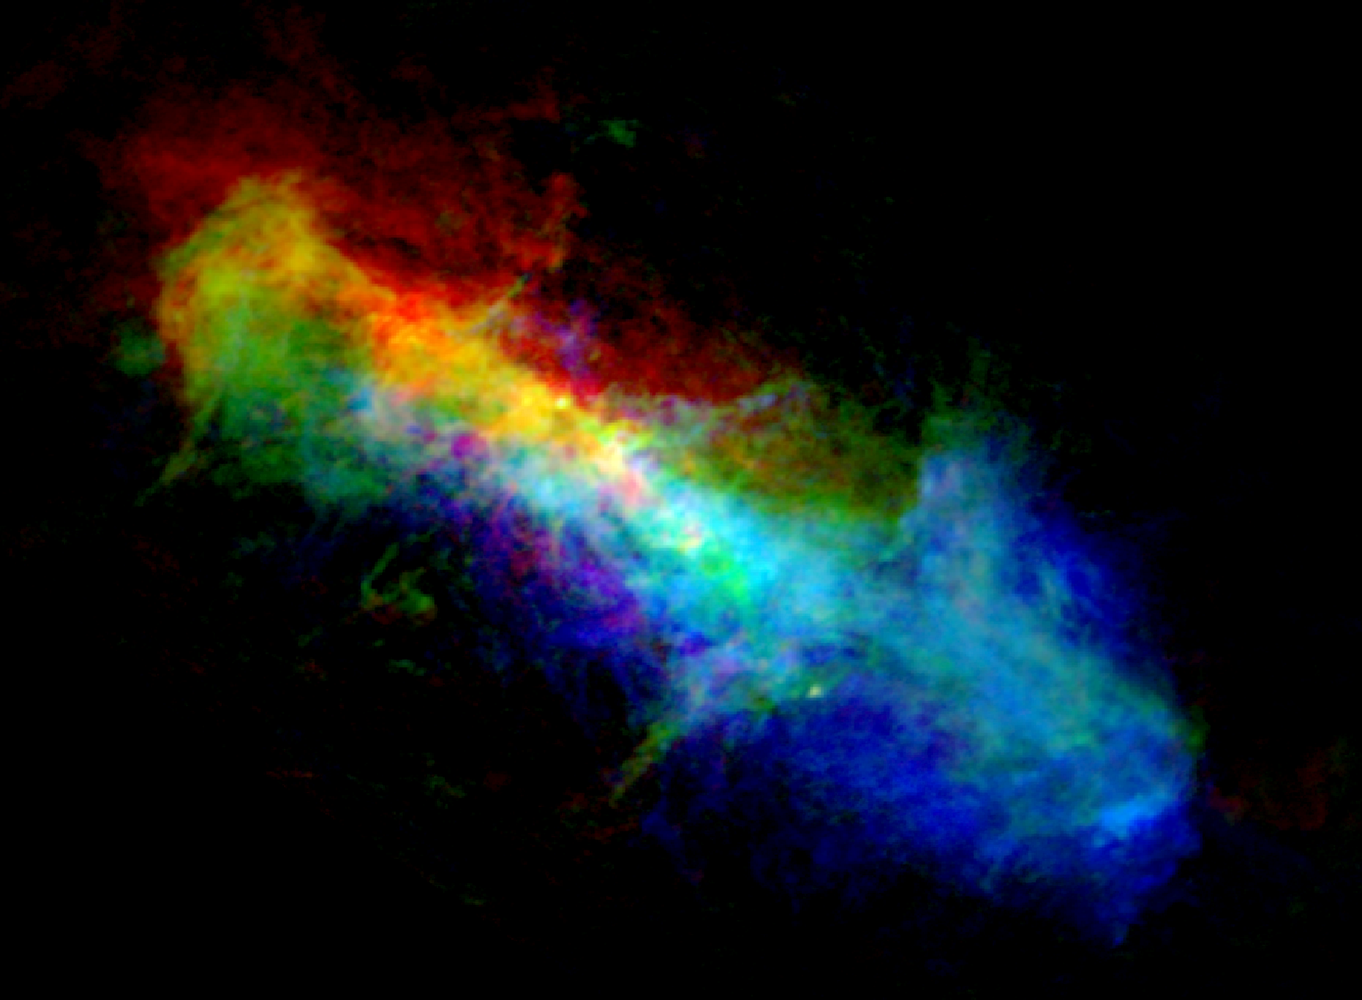
\includegraphics[width=\linewidth]{images/chapters/papers/outflow_catalog/CO32_false_color.png}
	\caption[Colorcoded velocity structure]{\co32 emission in the central $\sim1$\,kpc of \ngc253 colorcoded by velocity. Gas at the systemic velocity ($230-270$\,\kms) is shown in green while the redshifted ($\GTR 270$\,\kms) and blueshifted ($\LESS 230$\,\kms) emission in shown in the respective color. This choice of velocity intervals highlights the disturbed velocity field and prominently features the molecular streamers perpendicular to the projected disk.
	Note that this image shows the full dataset as presented in Chapter~\ref{chapter: outflow} at 2.5\,pc resolution while the analysis in this chapter is based on earlier observations with 7.5\,pc resolution.
	}\label{outflow catalog: figure: false color}
\end{figure*}


%%%%%%%%%%%%%%%%%%%%%%%%%%%%%%%%%%%%%%%%%%%%%%%%%%%%%%%%%%%%%%%%%%%%%%%%%%%%%%%%%%%%%%%%%%%%%%%%%%%%
%%%%%%%%%%%%%%%%%%%%%%%%%%%%%%%%%%%%%%%%%%%%%%%%%%%%%%%%%%%%%%%%%%%%%%%%%%%%%%%%%%%%%%%%%%%%%%%%%%%%

\section{Data reduction and imaging}

Obtaining a full ALMA dataset including multiple array configurations and total power data requires a substantial amount of time. The analysis presented in this chapter was thus conducted while the observation program was still ongoing and the highest resolution data (12\,m extended configuration) as well as the single dish data (total power array) was not yet observed. The following data therefore represent a subset of the complete dataset shown in Chapter~\ref{chapter: outflow}.

The observational setup is the same as for the full dataset with 7.6\,GHz spectral coverage (LSB: $342.0-345.8$\,GHz, USB: $353.9-357.7$\,GHz) in 976.6\,kHz channels (corresponding to 0.8\,\kms) and a linear four pointing mosaic covering the central $\sim750$\,pc of \ngc253. 
The observations were carried out in the compact configuration of the 12\,m array (baselines $15.1-83.5$\,m) in mid 2016 (12-Apr-2016, 23-Apr-2016, 17-Jun-2016, 27-Jun-2016) with typically 36~antennas and a total 2.6\,h on-source observation time.
The calibrators are: J0006-0623 (bandpass); J0038-2459 (complex gain); the asteroid Pallas (absolute flux density); J0104-2416, J0106-2718 (both WVR). The visibilities are calibrated using the ALMA cycle 3 pipeline in \casa 4.6.0 and the delivered calibration script.

In order to image the spectral lines, the continuum is subtracted using a first order polynomial fitted to the channels that do not contain strong spectral lines. At this resolution, we detect $\sim21$ spectral lines aside from the four strong lines \co32, \hcn, \hco and \cs. However, these lines are weak and only detected towards the central continuum sources (cf. Chapter~\ref{chapter: SSCs}) which is why they do not affect the overall continuum fit and subtraction.

For obtaining the final images and data cubes, we employ a multi-stage masking and \clean process. This ensures that \clean converges reliably and confines \clean masks to regions of real emission. We run an initial multi-scale \clean to $5\sigma$ with the rms noise level $\sigma = 75$\,mK of the dirty image without any spatial constraints. A mask that contains all pixels at $\GTR 2.5\sigma$ and enlarged to also include the surrounding $\sim0.5$\arcsec defines the \clean mask for the final multi-scale \clean run. In this final run (scales [0,3,9,27] with pixel size 0.1\arcsec), we clean the detected emission to $2.5\sigma$. 
All imaging tasks were carried out in \casa 4.6.0 with natural weighting and 2\,\kms channel width, imaging 500\kms centered on the redshifted ($v_\mathrm{sys} = 250$\,\kms) rest frequency. 
The noise in the final image is 75\,mK (1.35\,m\jybeam) in a 2.0\,\kms channel. The beam size is $0.48\arcsec \times 0.38\arcsec$ which corresponds to 8.1\,pc $\times$ 6.4\,pc at the distance of NGC 253.


\begin{table}
    \centering
    \begin{threeparttable}
    	\caption{Observation and image parameters.
    	\label{outflow catalog: table: image parameters}}
    % 	\footnotesize
        \begin{tabular}{ll}
            \toprule
            \ngc253                                                         \\
            \midrule
            distance            & 3.5\,Mpc                                  \\
            $v_\mathrm{sys}$    & 250\,\kms                                 \\ 
            \midrule
            Observations                                                    \\
            \midrule
        	project code        & 2015.1.00274.S                            \\
        	configuration       & 12\,m array, compact                      \\
        	baselines           & $15.1-83.5$\,m                            \\
        	spectral coverage   & $342.0-345.8$\,GHz                        \\
        	                    & $353.9-357.7$\,GHz                        \\
        	\midrule
        	Imaging                                                         \\
        	\midrule
        	beam                & $0.48\arcsec \times 0.38\arcsec$          \\
        	                    & 8.1\,pc $\times$ 6.4\,pc                  \\
        	channel width       & 2.0\,\kms                                 \\
        	rms noise           & 75\,mK                                    \\
        	                    & 1.35\,m\jybeam                            \\
            \bottomrule
        \end{tabular}
    \end{threeparttable}
\end{table}


%%%%%%%%%%%%%%%%%%%%%%%%%%%%%%%%%%%%%%%%%%%%%%%%%%%%%%%%%%%%%%%%%%%%%%%%%%%%%%%%%%%%%%%%%%%%%%%%%%%%
%%%%%%%%%%%%%%%%%%%%%%%%%%%%%%%%%%%%%%%%%%%%%%%%%%%%%%%%%%%%%%%%%%%%%%%%%%%%%%%%%%%%%%%%%%%%%%%%%%%%

\section{Construction on an outflow catalog}\label{outflow catalog: section: construction}

The identification of outflow candidates is based on visual inspection and their physical properties:
apparent filaments of high aspect ratio visible in channel maps (Figure~\ref{outflow: figure: CO channel map}) and integrated intensity (Figure~\ref{outflow: figure: CO moment maps}a) as well as higher velocity dispersion than the surrounding due to blending of a second kinematic component (Figs.~\ref{outflow: figure: CO moment maps}c, \ref{outflow: figure: co pV}). Potential outflows are those structures that contain gas at velocities outside the range of the rotating disk (cf. Section~\ref{outflow: section: disk separation}).

We identify 11 outflow candidates that are marked with approximate length and position angle in Figure~\ref{outflow catalog: figure: outflow catalog}. Names (o1 to o11) are assigned clockwise starting at the most prominent outflow, the south-west (SW) streamer. Annotated pV diagrams for the outflow candidates are given in Figure~\ref{outflow catalog: figure: outflow catalog pV}.
There is significant overlap with the ``features consistent with outflowing gas'' defined in \co21 by \citet{2018ApJ...867..111Z}: the SW streamer (o1 in this work) corresponds to SWS $1-3$ in Zschaechner et al. and our outflow candidates o3, o4, o8, o7 and o9/o10 correspond to the points OF$1-5$, respectively.

For each outflow candidate, we generate a mask in position-position-velocity (ppV) space with an intensity cut at $5\sigma$ rms noise level. For a projection of this mask onto the outflow major axis/velocity plane, see the shaded regions in Figure~\ref{outflow catalog: figure: outflow catalog pV}.


\paragraph{Size}
For each of these outflow candidates, we estimate the projected length (width) as the greatest extent along the long (short) dimension of the candidate. The projected extent is derived from the integrated intensity map of the $5\sigma$ (375\,mK) masked outflow candidate.

\paragraph{Orientation}
Orientation denotes the position angle (PA) of the outflow candidate's long axis (length) in the convention north to east. For reference, the molecular disk in \ngc253 is oriented at $\mathrm{PA_{maj}} = 55^\circ$ and $\mathrm{PA_{min}} = 145^\circ$ for the major and minor axis, respectively.

\paragraph{Mass}
We derive the molecular gas mass of the outflow candidates from the ppV $5\sigma$ masked integrated intensity. Following \citet{2013ARA&A..51..207B}, we adopt a starburst conversion factor X$_{CO} = 0.5 \times 10^{20}$\,\sqcm\,K$^{-1}$\,\kms and correct for the contribution of helium.

\paragraph{Velocity information}
Similar to the spatial extent of the outflow candidates, it is possible to estimate the velocity ranges over which the candidates can be traced. This is done in pV diagrams calculated from the data cube masked at the $5\sigma$-level.

We measure the velocity dispersion as the mean velocity dispersion (intensity-weighted second moment) over the ppV mask defining each outflow candidate.

Within the masked pV diagram of each candidate, we fit the median velocity (red line in Figure~\ref{outflow catalog: figure: outflow catalog pV}) with a first order polynomial (dashed red line in Figure~\ref{outflow catalog: figure: outflow catalog pV}) within the outflow mask.
For o8, we restrict the velocity gradient estimation to the linear part, ignoring the turn-over of the median velocity at the tip of this structure (offset $\GTR 0$\arcsec).
In o9 and o10, the pV structure splits into two arms affecting the estimation of median velocity, velocity dispersion and velocity gradient. In both cases, we follow the upper arm that connects linearly to the disk.
Note that these estimates are \emph{projected velocity gradients} that do not take geometrical effects like inclination and outflow cone angle into account.
\citet{2017ApJ...835..265W} demonstrated for the SW streamer that projected velocity gradients do not necessarily translate to velocity gradients in 3D space.

We also try to estimate the velocity of the disk gas at the position of the outflow candidate, i.e. within the shaded region in Figure~\ref{outflow catalog: figure: outflow catalog}, in order to interpret the observed gradients with respect to the local disk velocity.
This estimate must not be biased towards an outflow if the ratio of outflow to disk intensity is high (e.g. o1) to obtain a meaningful estimate of the disk velocity.
It also needs to be robust against sub-optimal choices of outflow masks, i.e. should not rely solely on the outflow masks.
These requirements are met by using the median velocity of a high SNR image cube (masked arbitrarily at $80\sigma$) where the ppV space covered by the fainter outflow candidates is masked out.
The velocity model obtained in Chapter~\ref{outflow: section: disk separation} is not a useful reference here because on the small spatial scales of the outflow candidates the local disk velocity can deviate from the large-scale model.

\paragraph{Outflow launching sites}
In trying to estimate the launching sites of the outflow candidates, two launching mechanisms need to be considered as they differ in pV structure:
If molecular gas is directly expelled by energetic processes like supernovae or forms in a directly ejected outflow of hot ionized gas through condensation, the observed molecular outflow has an initial velocity $v_0 \GTR 0$. Theoretical models suggest SN gas ejection velocities of $\sim 100$\,\kms creating a strong discontinuity between outflow and disk gas from which it is ejected. Simulations of large scale outflows like e.g. \citet{2018ApJ...853..173K} show ejection velocities $\GTR 20$\,\kms which would also be visible in our pV diagrams.
If ionized or neutral outflows launch molecular gas by entrainment at the edge or within an ionized/neutral outflow, no initial velocity should be observed ($v_0 = 0$) and the molecular gas should be more gradually accelerated.
The first picture causes the problem of launching dense molecular gas by energetic processes without destroying the gas (dissociating molecules, ionization).
In \ngc253, the outflow phases follow a stratification of an inner ionized, fast outflow, surrounded by a neutral outflow cone and another cone of molecular outflow \citep{2015ApJ...801...63M}. The gradual launching process with $v_0 = 0$, thus seems to be more likely. Also, the pV diagrams in Figure~\ref{outflow catalog: figure: outflow catalog pV} do not show a significant velocity offset but the outflow candidates seem to connect smoothly to the disk in most cases.

In o1, o2, o3, o4, o7, o8, o9 and o10, we can trace back the outflow candidates in ppV space to where they intersect the local disk with $v_0 =0$. Under the assumption of strictly linear movement, i.e. linear velocity gradient and linear movement in the plane of the sky, the outflow candidates would originate from these points which is a first estimate of the launching site. Figures~\ref{outflow catalog: figure: outflow catalog} and \ref{outflow catalog: figure: outflow catalog pV} indicate the launching sites with red crosses. Physically, this launching site estimation corresponds to outflows that are smoothly accelerated away from their launching site in a straight line.

\paragraph{Kinetic energy}
With the kinematic structure and masses, it is possible to estimate the kinetic energy for the outflow candidates in two ways.
The internal kinetic energy measured by the velocity dispersion of the outflow candidate can be calculated given the ppV masks and estimated as $\frac{m}{2} \sigma^2$. This energy estimate is referred to as $\mathrm{E}_{kin,disp}$ in Table~\ref{outflow catalog: table: outflow catalog}.
If a launching site can be reconstructed it is also possible to calculate the bulk kinetic energy of the outflowing gas relative to that zero point by integrating along the outflow candidate $\mathrm{E}_{kin,launch} = \int \frac{m}{2} \left( v_i - v_{launch} \right)^2 \mathrm{d}v_i$.

\paragraph{Dynamical age}
The dynamical age of an outflow can be estimated by the time it took the tip to reach its current position. As before, the velocity gradient $v'$ in pV space is taken to be constant as was fitted to the median velocities.
The derivation of meaningful time scales require the following assumptions on the 3D structure.
As the simplest assumption, we take all outflow candidates to lie perpendicular to the disk because the true angle cannot be reconstructed and most candidates are found to lie roughly perpendicular to the projected disk (see the discussion below). The projected quantities offset $x_{proj}$, radial velocity $v_{rad}$ and velocity gradient $v'$ can then be deprojected when taking inclination $i$ into account:

\begin{eqnarray}
	x_{3D} &=& \frac{x_{proj}}{\sin i} \nonumber\\
	v_{3D} &=& \frac{v_{rad}}{\cos i} \nonumber\\
	v'_{3D} &=& \frac{\mathrm{d}v_{rad}}{\mathrm{d}x_{proj}} = v'_{proj} \times \tan i \nonumber
\end{eqnarray}

The dynamical age is given by the distance $x_{3D}$ between base and tip of an outflow candidate and the fitted velocity gradient. The base is either the launching site or the inner edge of the outflow mask if no launching site could be reconstructed.

\begin{displaymath}
	\mathrm{t}_{dyn}\,[\mathrm{Myr}] = 0.98 \times \frac{\ln \left( x_{3D}\,[\mathrm{pc}] \right)}{v'_{3D}\,[\mathrm{km}\,\mathrm{s}^{-1}\,\mathrm{pc}^{-1}]}
\end{displaymath}

The prefactor 0.98 handles the unit conversions.

\begin{figure}[t]
	\centering
	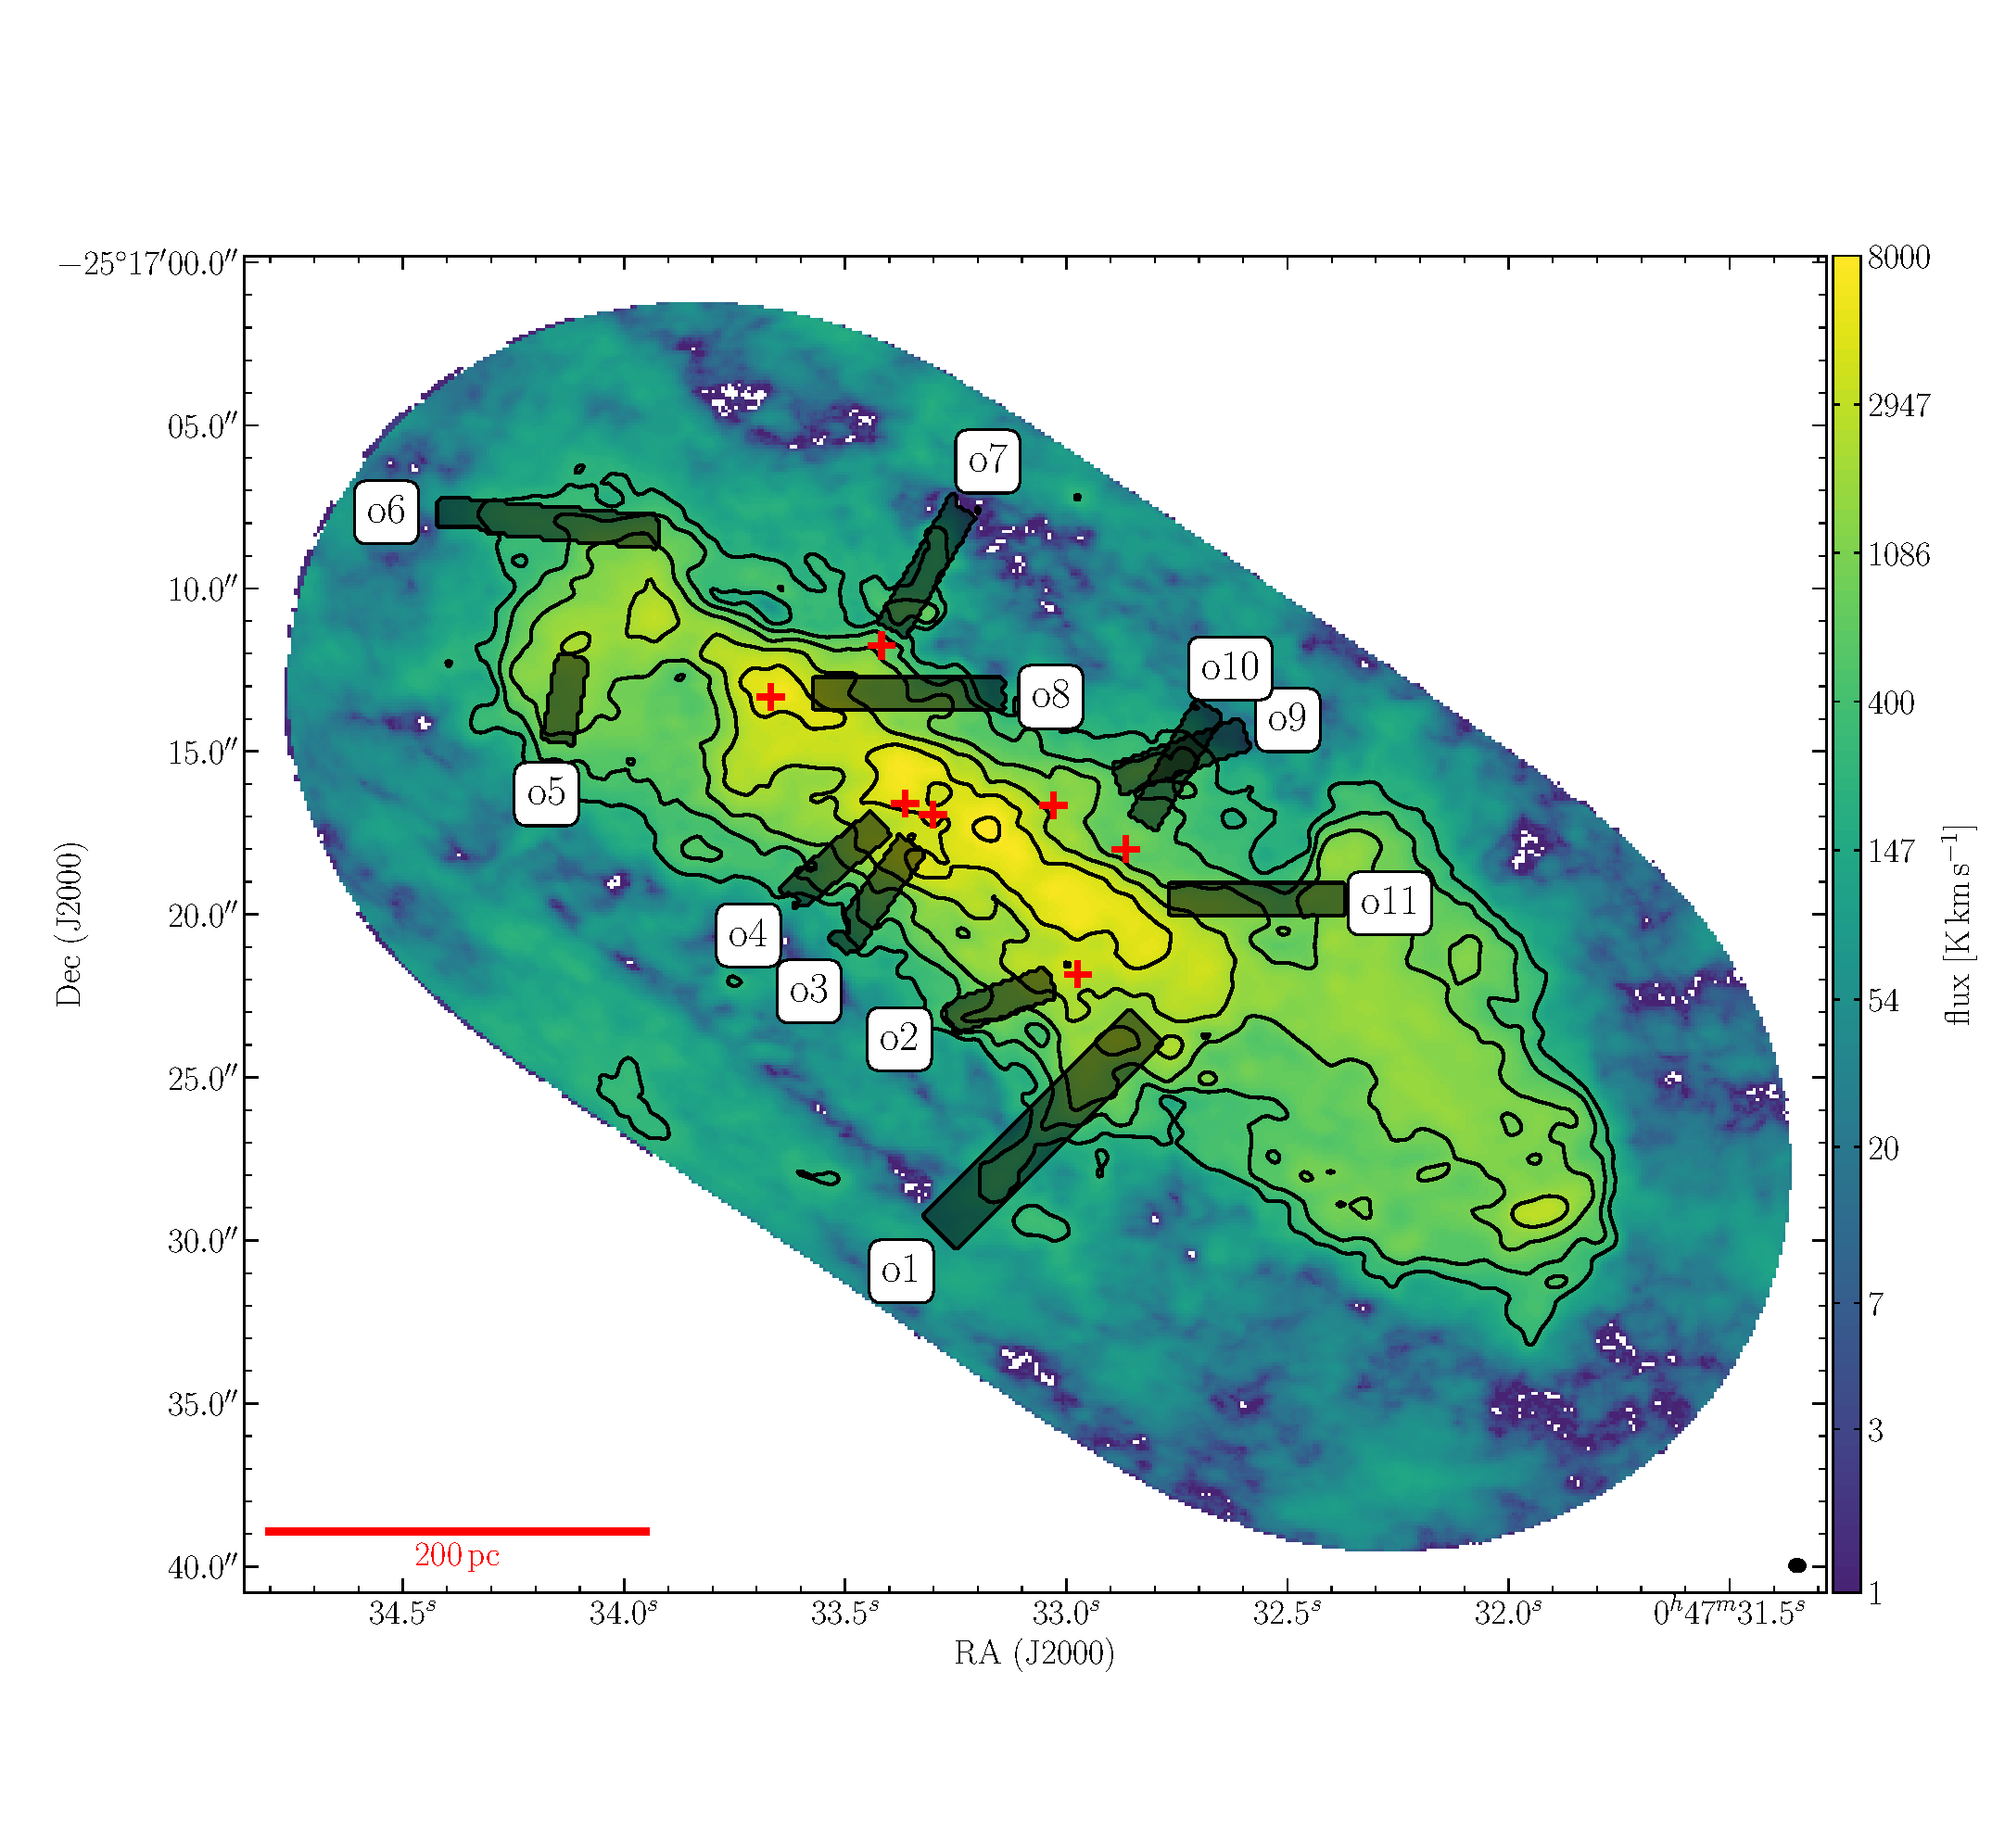
\includegraphics[width=\linewidth]{images/chapters/papers/outflow_catalog/fig7.pdf}
	\caption[Overview of identified small scale outflow candidates]{Positions of identified outflows as listed in Table~\ref{outflow catalog: table: outflow catalog}. The background shows the \co32 integrated intensity. Not all outflow candidates show up clearly in this map due to blending for fore-/background emission. However, they can be identified in position-velocity diagrams, which are calculated along each outflow (Figure~\ref{outflow catalog: figure: outflow catalog pV}) . The length of the overlaid boxes reflect the length over which the outflows can be traced in pV space. In the cases where the outflow can be traced back to the disk the potential launching sites are marked by red crosses.}
	\label{outflow catalog: figure: outflow catalog}
\end{figure}

\begin{figure}[p]
	\centering
	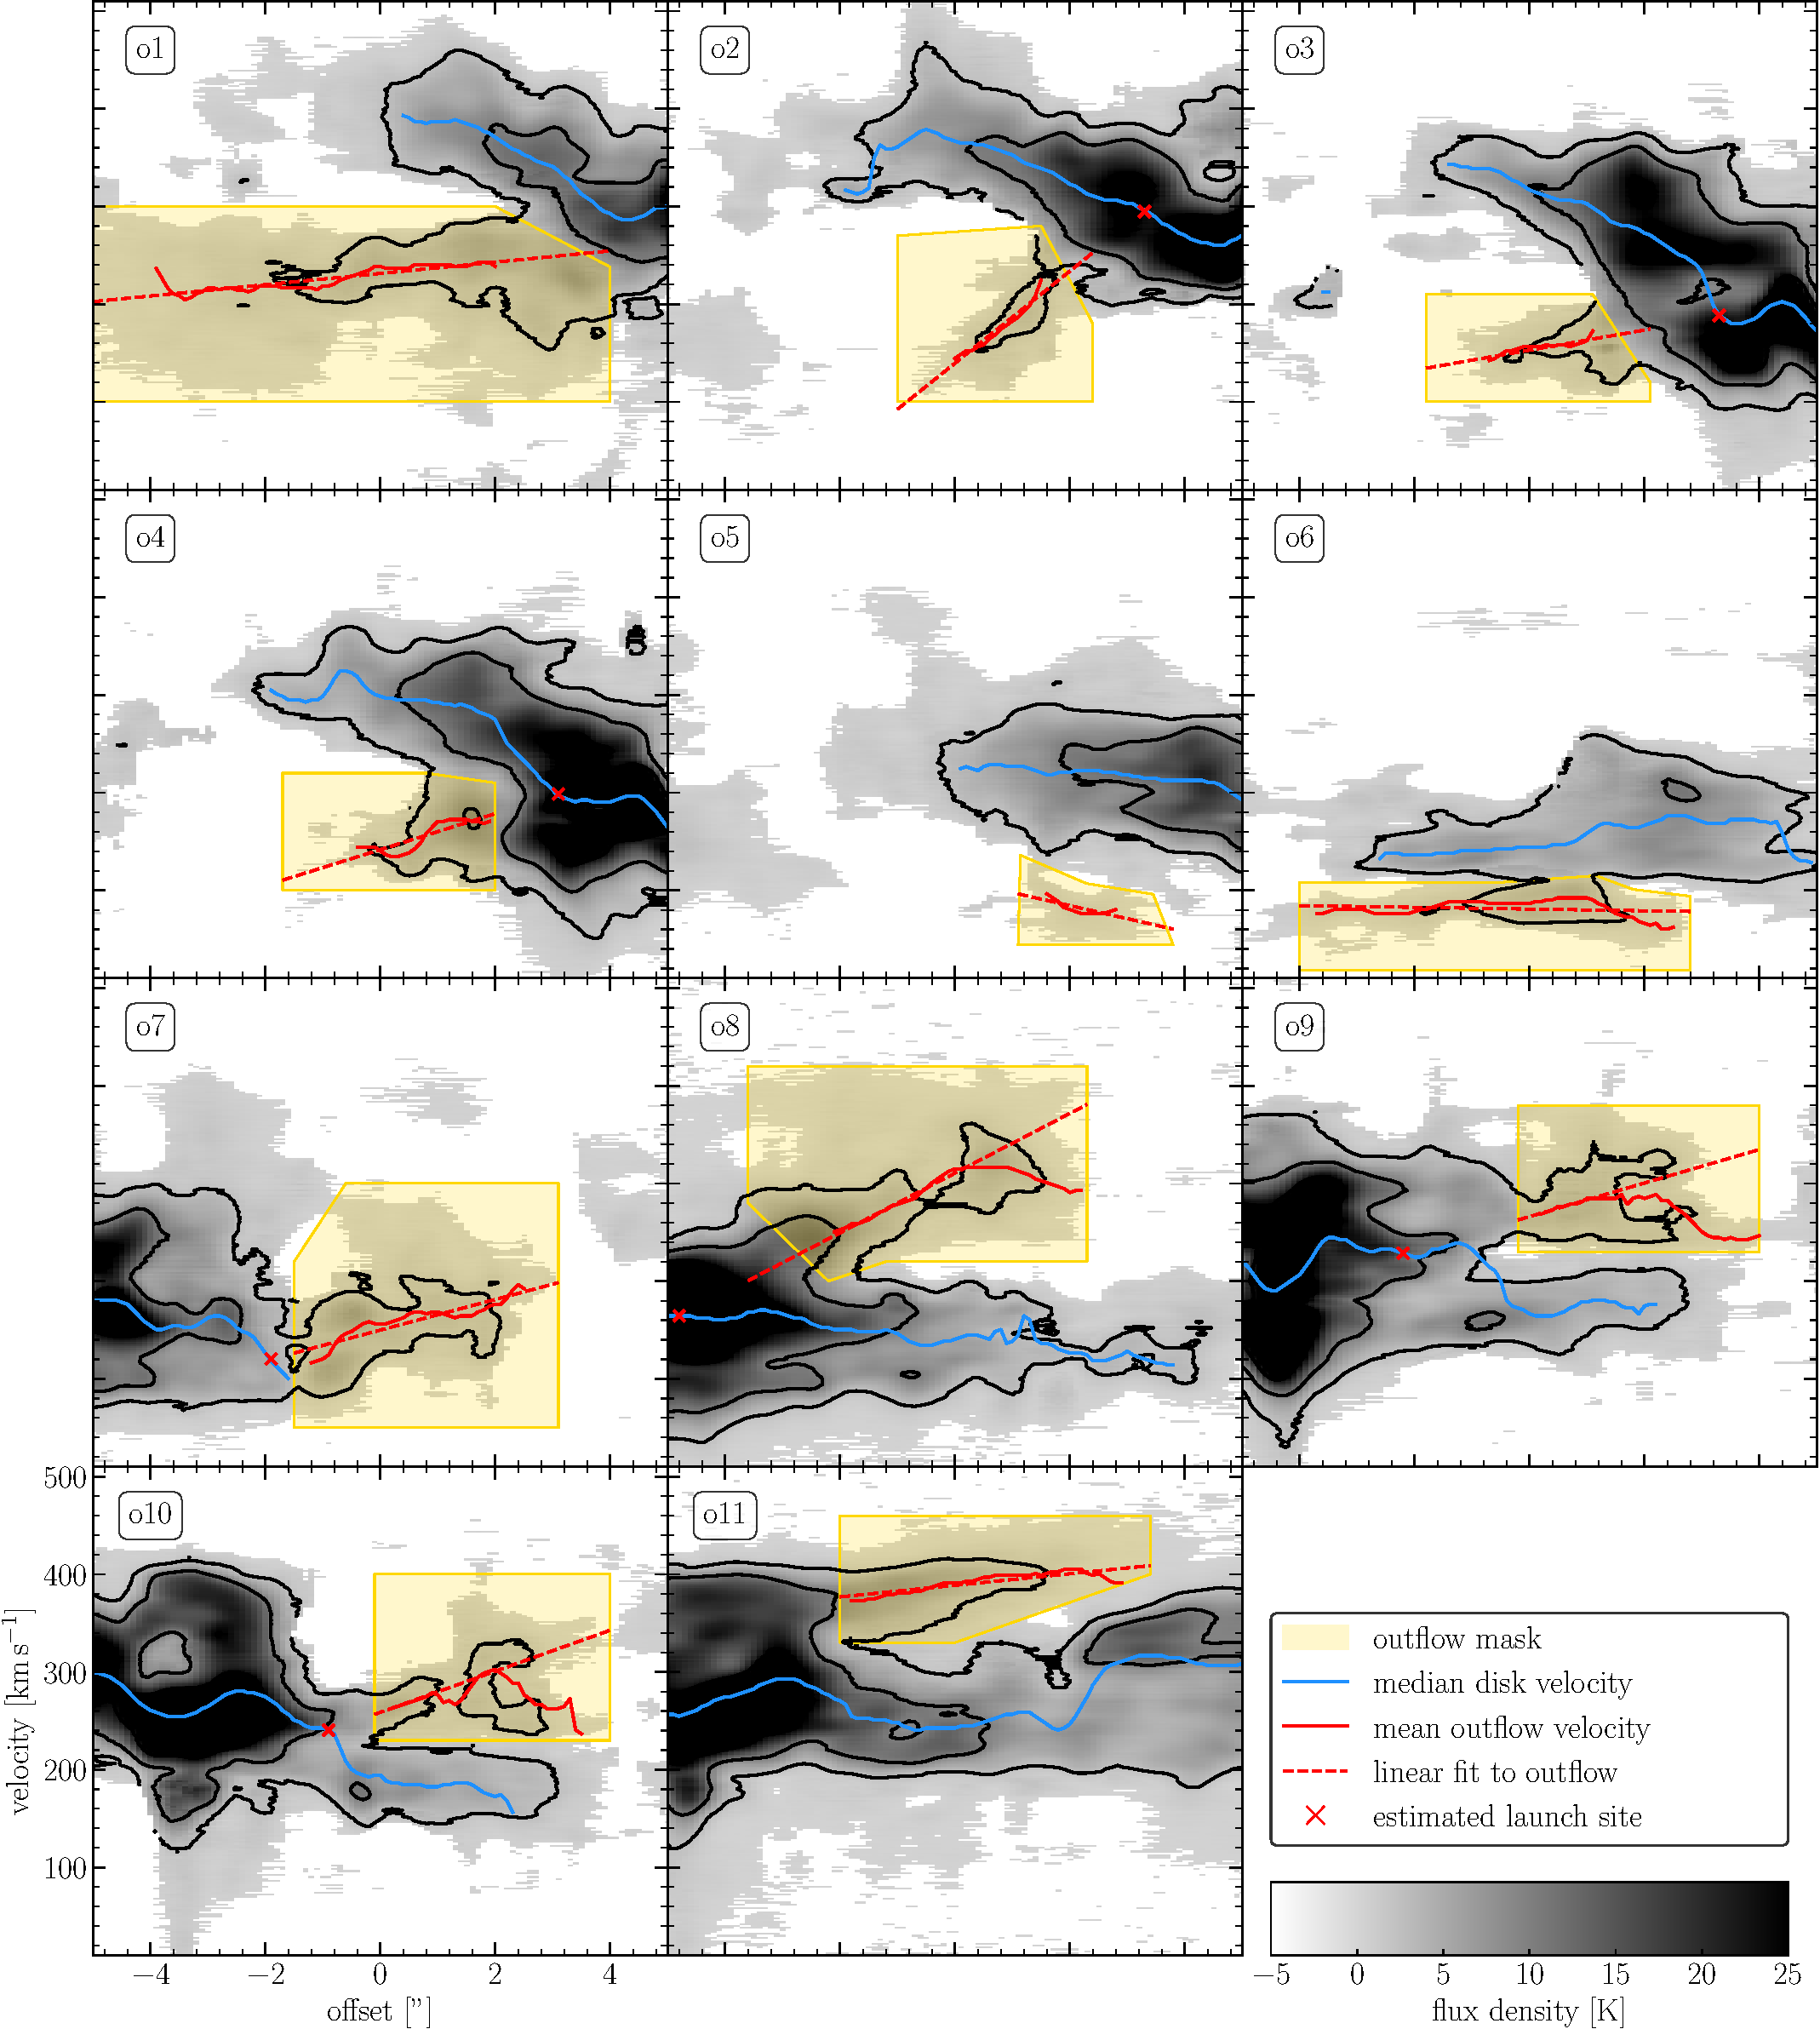
\includegraphics[width=\linewidth]{images/chapters/papers/outflow_catalog/fig8.pdf}
	\caption[Position-velocity diagrams of outflow candidates]{Position-velocity diagrams of the \co32 outflow candidates o1 to o11 masked at $5 \sigma$ (background grey scale images, saturated at 25\,K). The regions considered to be outflows is highlighted by golden outlines and shadings. Blue lines indicate the local median velocity of the molecular disk. Red lines indicate the local mean velocity in the outflow candidates that are fitted as indicated by dashed red lines. If the fitted outflow velocity gradient intersect the local disk, the intersection is marked by a red cross (o2, o3, o4, o7, o8, o9, o10).}
	\label{outflow catalog: figure: outflow catalog pV}
\end{figure}


%%%%%%%%%%%%%%%%%%%%%%%%%%%%%%%%%%%%%%%%%%%%%%%%%%%%%%%%%%%%%%%%%%%%%%%%%%%%%%%%%%%%%%%%%%%%%%%%%%%%
%%%%%%%%%%%%%%%%%%%%%%%%%%%%%%%%%%%%%%%%%%%%%%%%%%%%%%%%%%%%%%%%%%%%%%%%%%%%%%%%%%%%%%%%%%%%%%%%%%%%

\section{Outflow statistics}\label{outflow catalog: section: statistics}

Physical properties of the outflow candidates are listed in Table~\ref{outflow catalog: table: outflow catalog} and briefly discussed in the following.

\paragraph{Size}
The projected lengths of the outflow candidates range from 1.9\arcsec (32\,pc) to 11.0\arcsec (187\,pc) with a mean 4.9\arcsec (83\,pc). In all cases, the mean width is small $0.5"$ (8\,pc) to $1.4"$ (24\,pc) and close to the resolution limit.

\paragraph{Orientation}
Typically, the structures are oriented close to perpendicular to the plane of the star forming gas disk. The deviation from the minor axis is $\Delta\mathrm{PA} = 0^\circ - 35^\circ$ to the south and $\Delta\mathrm{PA} = 5^\circ - 55^\circ$ to the north.
Candidate o6 is almost parallel to the major axis and hence is unlikely to be an outflow driven by stellar feedback of the starburst.

\paragraph{Velocity range}
Derived velocity ranges over which the outflow candidates can be traced at the $5\sigma$-level are consistent for outflows on each side of the plane, $\sim 100-250$\,\kms to the south, $\sim 230-360$\,\kms to the north and thus symmetric to the systemic velocity of 250\,\kms.

\paragraph{Mass}
Individual mass estimates range between $5.31 \times 10^3$\,\Msun for the small o5 and $1.12 \times 10^6$\,\Msun for the large and massive SW streamer. The summed outflowing mass without o5 and o6 is $1.91\times 10^6$\,\Msun which is about a third of the lower limit found by \citet[][$6.6 \times 10^6$\,\Msun]{2013Natur.499..450B}. Such a fraction is reasonable given that this mass sums up only 9 distinctive features not considering less obvious features and diffuse outflows. 
The combined streamer masses amount to $\sim 5-10$\% of the total outflow mass in \co10 and \co21 in \citet[Chapter~\ref{chapter: outflow}]{2019ApJ...881...43K}. A more meaningful comparison is the \co32 outflow mass of $8.3 \times 10^6$ since the lower CO line observations cover significantly larger areas. Within $\sim 100$\,pc of the disk, the likely outflowing streamers (o1--o4, o7--o11) contribute $\sim 25$\% to the outflowing molecular gas mass. Adopting the proportion of $\sim 50$\% diffuse and $\sim 50$\% localized outflow as indicated in \citet[Chapter~\ref{chapter: outflow}]{2019ApJ...881...43K}, the streamer identified here make up already half of the localized outflowing \co32 mass.

\paragraph{Velocity gradient}
We find a wide variety of velocity gradients among the outflow candidates. All are accelerating with respect to the local disk velocity with the exception of o5 and o6 that are offset from but parallel to the disk velocity.
In the SW streamer (o1), the gradient is 0.34\,\kms\,pc$^{-1}$ which is almost identical to \citet[$0.36$\,\kms\,pc$^{-1}$]{2017ApJ...835..265W} who were able to trace this outflow further out in \co10.
Adopting their projection correction of a factor of $\sim 3$, our best estimate for the geometry corrected velocity gradient is 1.02\,\kms\,pc$^{-1}$, i.e. the molecular gas traced by \co32 is accelerating away from the disk.
Good estimates of the velocity gradients are obtained for o2 to o8 and o11, most of them accelerating faster than o1 at $0.36$\,\kms\,pc$^{-1}$ to $\sim 2.78$\,\kms\,pc$^{-1}$ in projection. Depending on the unknown geometry of each individual outflow candidate, the 3D velocity gradient can be greater by factors of unity to a few.
Gradients of the other candidates need special discussion as they are affected by several effects.
In both o9 and o10, the proposed outflow splits into two parts that are at constant velocity and accelerating at $\GTRSIM 1.0$\,\kms\,pc$^{-1}$ which is not well reflected by a combined fit.
The origin of the splitting cannot be inferred from the data at hand and must be addressed in a more detailed study.
The velocity of o5 and o6 is oriented parallel to that of the disk, so they cannot be considered outflows but rather a second kinematic component, e.g. a foreground cloud.

\paragraph{Launching sites}
The projected launching sites defined by tracing back the velocity gradient to the disk lie close to the star forming disk midplane for o3, o4 and o8.
Furthermore, the launching sites of o2, o3, o4, o9 and o10 can be considered close (offset $\LESSSIM 1\arcsec$ or $\LESSSIM 20$\,pc) to sites of recent star formation in star forming massive clumps \citep{2017ApJ...849...81A} and (proto-) SSCs \citep{2018ApJ...869..126L}.
Note that the positional accuracy of the launching site estimation depends strongly on the velocity gradient and is $0.5\arcsec-1.0\arcsec$. Furthermore, the back-traced launching sites are projected positions and do not necessarily lie close to the clumps and SSCs in 3D space. The inferred proximity, however, is reassuring.
The SSCs currently undergoing star formation are most likely not the launching sites of the observed outflows because of feedback delay. The amount of time required to form the observed outflows (kinematic ages $\sim$ Myr, see below) and the time delay until the first supernovae explode after the onset of star formation (several Myr) is older than the age of the (proto-)SSCs. Recently, \citet{2020MNRAS.491.4573R} age-dated half of the 14 (proto-)SSCs in \ngc253 to $\LESSSIM 1$\,Myr while the other half is still on the zero-age main sequence and thus also still very young. 
The outflow candidate launching site are then not expected to match exactly the locations of current clusters. Older clusters that might have launched the observed outflow candidates should have formed at similar locations within the disk. An approximate correspondence between sites of on-going star formation and the launching sites is therefore expected.

\paragraph{Velocity dispersion}
Velocity dispersions within the outflow candidates vary by a factor of $\sim 2$ across the candidates with the highest dispersions of $\GTR 30$\,\kms found in the most massive outflows o1, o7 and o8.
The low dispersions of $\sim 13$\,\kms in o5 and o6 support the idea that these are of different origin than the other outflow candidates.
\citet{2017ApJ...835..265W} state a somewhat wider $35 - 40$\,\kms for the SW streamer (o1) in \co10 than the 34.1\,\kms that we find in \co32 which is potentially due to the higher excitation state.

\paragraph{Kinetic energy}
The internal kinetic energy derived from the velocity dispersion $E_\mathrm{kin,disp}$ is typically a few times $10^{49}$\,erg. o2 and o3 are significantly less energized owing to their low mass. Due to their low velocity dispersion, o5 and o6 also contain low amounts of internal kinetic energy.

The bulk kinetic energy of an outflow $\mathrm{E}_{kin,launch}$ can be calculated only for the candidates for which a launching site can be estimated and varies strongly between $\sim 6 \times 10^{48}$\,erg (o3) and $\GTR  5 \times 10^{50}$\,erg (o8).
The very high energy in o8 is explained by being massive and having a strong velocity gradient; the line-of-sight velocity at its tip is $\sim 160$\,\kms faster than at the estimated launching point.

Comparing the two energy estimates, o2 and o8 are dominated by bulk kinetic energy with $E_\mathrm{kin,launch} \GTRSIM 10 \times E_\mathrm{kin,disp}$.
In the other cases where both energies could be calculated, $E_\mathrm{kin,disp} \simeq E_\mathrm{kin,launch}$ to a surprising precision of a factor $\LESS 2-3$.
This results argues for approximate energy partition between internal and bulk kinetic energy in a typical molecular streamer.

\paragraph{Dynamical age}
For o5 and o6, no meaningful dynamical age can be calculated because their velocity gradients are close to parallel to the local disk velocity.
For the other candidates, the short ages of $\sim 1.2$\,Myr on average indicate that the observed molecular streamers are mostly a young feature.
o1 and o11, however, are significantly older with 3.0 and 2.5\,Myr, respectively.

For o1, \citet{2017ApJ...835..265W} report an age of $\sim 1$\,Myr with a projection correction factor of $\sim 3$ as given by \citet{2013Natur.499..450B}.
Our assumption of a perpendicular outflow translates to a projection correction of $\left[ \sin \left( i-90^\circ \right) \right]^{-1} \sim 5$.
If we also adopt a projection correction of 3 instead of 5, the dynamical age of o1 would be 1.8\,Myr instead of 3.0\,Myr.

We expect age uncertainties of a factor of at least $\sim 2$ due to the unknown geometry alone. A factor of two translates to a deviation from perpendicular orientation by just $\sim 10^\circ$. Even when considering this uncertainty, the molecular outflow candidates are kinematically young features and likely all younger than a few Myr.

\begin{sidewaystable}
% \begin{table}
	\centering
% 	\tablewidth{\textwidth}
    \begin{threeparttable}
	    \caption[Catalog of outflow features]{Catalog of the outflows indicated in Figure~\ref{outflow catalog: figure: outflow catalog}.
	        \label{outflow catalog: table: outflow catalog}}
%	    \vspace{}
    \begin{tabular}{cccccccccccc}
        \toprule
        \multirow{2}{*}{name} & mid point: RA, DEC & length\tnote{a} & width\tnote{a} & PA\tnote{b} & velocity\tnote{c} & mass\tnote{d} & gradient\tnote{e} & dispersion\tnote{f} & E$_{kin,disp}$\tnote{g} & E$_{kin,launch}$\tnote{h} & t$_{dyn}$\tnote{i}\\
		& (J2000) & ["] & ["] & [$^\circ$] & [km\,s$^{-1}$] & [\Msun] & [km\,s$^{-1}$\,pc$^{-1}$] & [km\,s$^{-1}$] & [erg] & [erg] & [Myr]\\
        \midrule
    	o1  & 00:47:33.034, -25:17:26.352 & 11.0 & 1.1 & 135 & 180-250 & $1.12 \times 10^6$ & 0.34  & 34.1 & $5.05 \times 10^{49}$ & & 3.0\\
	    o2  & 00:47:33.204, -25:17:22.970 & 2.8  & 0.9 & 110 & 100-200 & $3.21 \times 10^4$ & 2.78  & 21.8 & $6.65 \times 10^{48}$ & $1.16 \times 10^{50}$ & 0.3\\
	    o3  & 00:47:33.442, -25:17:19.660 & 3.0  & 0.8 & 145 & 126-174 & $3.99 \times 10^4$ & 0.61  & 16.8 & $2.11 \times 10^{48}$ & $6.01 \times 10^{48}$ & 1.5\\
	    o4  & 00:47:33.538, -25:17:18.581 & 2.6  & 0.5 & 130 & 120-160 & $7.61 \times 10^4$ & 1.09  & 18.6 & $1.23 \times 10^{49}$ & $3.01 \times 10^{49}$ & 0.8\\
	    o5  & 00:47:34.170, -25:17:15.919 & 1.9  & 0.9 & 170 & 180-250 & $5.31 \times 10^3$ & -0.78 & 12.7 & $3.61 \times 10^{47}$ & & \\
	    o6  & 00:47:34.133, -25:17:08.148 & 7.1  & 1.4 & 85  & 60-170  & $9.64 \times 10^4$ & -0.04 & 13.3 & $3.44 \times 10^{48}$ & & \\
	    o7  & 00:47:33.347, -25:17:10.091 & 4.2  & 1.1 & 330 & 80-230  & $1.22 \times 10^5$ & 0.91  & 34.4 & $4.25 \times 10^{49}$ & $4.47 \times 10^{49}$ & 1.0\\
	    o8  & 00:47:33.315, -25:17:13.329 & 5.2  & 0.8 & 270 & 260-360 & $2.57 \times 10^5$ & 1.80  & 32.6 & $4.63 \times 10^{49}$ & $5.40 \times 10^{50}$ & 0.5\\
	    o9  & 00:47:32.880, -25:17:15.919 & 2.9  & 1.1 & 290 & 230-350 & $7.69 \times 10^4$ & 1.03  & 25.9 & $2.29 \times 10^{49}$ & $6.33 \times 10^{49}$ & 0.9\\
	    o10 & 00:47:32.832, -25:17:17.214 & 4.1  & 1.2 & 330 & 240-300 & $6.02 \times 10^4$ & 1.22  & 28.9 & $1.38 \times 10^{49}$ & $2.68 \times 10^{49}$ & 0.7\\
	    o11 & 00:47:32.630, -25:17:19.660 & 4.5  & 0.8 & 270 & 260-330 & $1.25 \times 10^5$ & 0.36  & 19.0 & $1.04 \times 10^{49}$ & & 2.5\\
	    \midrule
	    mean/sum$^j$ &                    & 4.9  & 1.0 &     &         & $1.90 \times 10^6$ & 1.13  & 25.7 & $2.31 \times 10^{49}$ & $1.09 \times 10^{50}$ & 1.2\\
        \bottomrule
    \end{tabular}
    \vspace{0.5em}
	\begin{tablenotes}
		\item[a] projected range over which the outflow can be traced in the channel maps at the $5 \sigma$ level
		\item[b] north to east
		\item[c] velocity range in which the outflow can be traced in the channel maps at the $5 \sigma$ level
		\item[d] H$_2$ mass assuming a starburst $\mathrm{X}_{CO} = 0.5 \times 10^{20}$\,\sqcm
		\item[e] velocity gradient along the outflow
		\item[f] mean dispersion per channel
		\item[g] kinetic energy derived from velocity dispersion
		\item[h] kinetic energy relative to the launching site
		\item[i] dynamical age of the outflow tip
		\item[j] without o5 and o6 which are considered not to be outflows (see text); for the mass, the sum instead of the mean is given
	\end{tablenotes}
	\end{threeparttable}
% \end{table}
\end{sidewaystable}

%%%%%%%%%%%%%%%%%%%%%%%%%%%%%%%%%%%%%%%%%%%%%%%%%%%%%%%%%%%%%%%%%%%%%%%%%%%%%%%%%%%%%%%%%%%%%%%%%%%%
%%%%%%%%%%%%%%%%%%%%%%%%%%%%%%%%%%%%%%%%%%%%%%%%%%%%%%%%%%%%%%%%%%%%%%%%%%%%%%%%%%%%%%%%%%%%%%%%%%%%

\section{Discussion}

The high resolution achievable with ALMA allows to detect a surprising level of substructure around the starburst in \ngc253. The previously highest resolution study in \citet[32\,pc spatial resolution]{2017ApJ...835..265W} could detect only the SW streamer as a localized feature close to the resolution limit.
The sample of molecular streamers in this work allows us to infer the typical properties and variations thereof. Although on a small statistical basis, trends can be inferred.

The kinetic and structural parameters of the 11 outflow candidates reveals that most of them indeed show evidence of being driven out from the starburst by feedback. Candidates o5 and o6 are likely not outflowing but other molecular clouds that do not kinematically match the disk and exhibit a high aspect ratio. Their location at the edge of the molecular disk towards the bar indicate that they could potentially be infalling molecular clouds. Due to the high inclination of \ngc253, o5 and o6 can also be fore-/background clouds off the midplane in the spiral arms.

The other candidates o1-o4 and o7-o11 are likely to be outflowing molecular structures. Their projected geometry and velocity structure are consistent with individual molecular clouds flowing away from a launching site in the disk while getting dispersed along the flow direction.
For o1 (SW streamer), the only streamer described before, our measurements match closely to the literature values. For the other outflowing streamers, we obtain plausible results lower than for o1, the most massive and largest streamer.

The formation of outflowing streamers is unclear and cannot be inferred from our analysis. Now that they are characterized, potential formation scenarios can be tested.
Each molecular streamer could be an independent collimated feature. The collimation of the outflowing gas down to $\leq 20$\,pc in this scenario is unclear. A potential collimation mechanisms may be the entrainment of molecular gas in an ionized flow after (super-)bubble breakout. Over-pressurized, ionized gas due to feedback is known to vent through channels of least resistance in the disk \citep[e.g.][]{2012ApJ...760..155K,2016MNRAS.456.3432G} that could entrain molecular gas. In that case, the streamers are the extension of feedback vents. 
More likely, however, is a scenario in which a large stratified outflow fragments. The multi-phase outflow cone in \ngc253 is thought to be radially stratified \citep[as shown in Figure~\ref{introduction: figure: star formation: outflow cone}]{2015ApJ...801...63M} with a thin shell of molecular gas surrounding the ionized outflow. Such a thin sheet of dense gas is unlikely to remain stable even on short timescales, but expected to fragment. The outflow cone would then break up into a set of narrow dense streamers. The remaining molecular gas in between the streamer might accrete locally onto the streamers or get dissociated/ionized quickly due to diminishing self-shielding against the adjacent ionized outflow.
Specialized, parsec scale resolution simulations and observations across all outflow gas phases will be required to reveal potential interactions.


%%%%%%%%%%%%%%%%%%%%%%%%%%%%%%%%%%%%%%%%%%%%%%%%%%%%%%%%%%%%%%%%%%%%%%%%%%%%%%%%%%%%%%%%%%%%%%%%%%%%
%%%%%%%%%%%%%%%%%%%%%%%%%%%%%%%%%%%%%%%%%%%%%%%%%%%%%%%%%%%%%%%%%%%%%%%%%%%%%%%%%%%%%%%%%%%%%%%%%%%%


\section{Summary}

We follow up the global look at the \ngc253 starburst outflow by a high-resolution look at individual, potentially outflowing, structures in \co32 that we refer to as streamers.
We identify eleven distinct features by eye, nine of which are kinematically consistent with being outflows and two potentially infalling GMCs.

\begin{enumerate}[noitemsep,topsep=0pt]

\item The outflows are close to perpendicular to the gas disk with mean projected sizes of $4.9\arcsec \times 1.0\arcsec$ ($83\,\mathrm{pc} \times 17\,\mathrm{pc}$).

\item The combined mass of the nine outflows is $1.9 \times 10^6$\,\Msun, about half of the mass in localized outflows found in \co32 in \citet[, Chapter~\ref{chapter: outflow}]{2019ApJ...881...43K}.
The outflows are accelerating away from the disk with a mean velocity gradient of 1.13\,\kms\,pc without projection correction.

\item By tracing back the outflow candidates to the disk, we are able to estimate the launching sites and find them to lie close to the major axis of the molecular disk and in five cases also close (offset $\sim 1\arcsec$ or $\sim 20$\,pc) to sites of current cluster formation.

\item Within the streamers, the mean velocity dispersion is $\sim 26$\,\kms which results in a typical turbulent energy of a few $10^{49}$\,erg.
If a launching site could be estimated, the bulk kinetic energy is typically a few times $10^{49}$\,erg but an order of magnitude higher for two streamers with particularly steep velocity gradients.
This result implies that streamers are typically in approximate energy equipartition between internal and bulk kinetic energy.

\item All streamers are kinematically young $\leq 3$\,Myr and typically $\sim 1$\,Myr old.

\end{enumerate}

Further high-resolution observations across the gas phases and simulations are required to reveal the formation mechanism of outflowing streamers.
%************************************************
\chapter{The Molecular ISM in the Super Star Clusters of the Starburst \ngc253}
\chaptermark{ISM in the SSCs of \ngc253}
\label{chapter: SSCs}
%************************************************

\begin{papernote}
This chapter including appendix~\ref{appendix: SSCs} comprises the article of the same title submitted the to Astrophysical Journal. The submitted paper has been reformatted to match the style of this thesis.
\end{papernote}

\begin{paperabstract}
We present submillimeter spectra of the (proto-)super star cluster (SSC) candidates in the starbursting center of the nearby galaxy \ngc253 identified by \citet{2018ApJ...869..126L}. The 2.5\,pc resolution of our ALMA cycle 3 observations approach the size of the SSCs and allows the study of physical and chemical properties of the molecular gas in these sources. 
In the 14 SSC sources and in the frequency ranges $342.0-345.8$\,GHz and $353.9-357.7$\,GHz we detect 55 lines belonging to 14 different chemical species. The SSCs differ significantly in chemical complexity, with the richest clusters showing 14 species and the least complex showing 5 species. We detect HCN isotopologues and isomers (H$^{13}$CN, HC$^{15}$N, H$^{15}$NC), abundant HC$_3$N, SO and S$^{18}$O, SO$_2$, and H$_2$CS. The gas ratios CO/HCN, CO/HCO$^+$ are low, $\sim 1-10$, implying high dense gas fractions in the SSCs.
Line ratio analyses suggests chemistry consistent with photon-dominated regions and mechanical heating. 
None of the SSCs near the galaxy center show line ratios that imply an X-ray dominated region, suggesting that heating by any (still unknown) AGN does not play a major role.
The gas temperatures are high in most sources, with an average rotational temperature of $\sim 130$\,K in SO$_2$. 
The widespread existence of vibrationally excited HCN and HC$_3$N transitions implies strong IR radiation fields, potentially trapped by a greenhouse effect due to high continuum opacities.
\end{paperabstract}


%%%%%%%%%%%%%%%%%%%%%%%%%%%%%%%%%%%%%%%%%%%%%%%%%%%%%%%%%%%%%%%%%%%%%%%%%%%%%%%%%%%%%%%%%%%%%%%%%%%%

\section{Introduction} \label{SSCs: section: introduction}

\defcitealias{2018ApJ...869..126L}{L18}

% SSCs
Super star clusters (SSCs) are massive ($\mathrm{M}_* \GTR  10^5$\,\Msun), compact ($\mathrm{R} \sim 1$\,pc) clusters of stars. They are frequently found in starbursts in the centers of galaxies or galaxy mergers, such as M~82, NCG~253 or the Antennae galaxies \citep[e.g.][]{1992AJ....103..691H,2003dhst.symp..153W,2005ApJ...621..278M,2010ARA&A..48..431P,2018ApJ...869..126L}. The stellar properties of SSCs are similar to Galactic globular clusters and thus SSCs might represent a younger generation of the same sort of stellar systems \citep[e.g.][]{2010ARA&A..48..431P}. The extreme conditions under which SSCs form are rare in the present-day universe but are thought to be common around the peak of the cosmic star formation rate history, the era when most of today's globular clusters formed. Hence, observations of forming SSCs might offer a glimpse into the physics of a mode of star formation common in the early universe.

% \ngc253
\ngc253 is one of the nearest starburst systems, at a distance of 3.5\,Mpc \citep{Rekola:2005ha}. It is considered one of the prototypical starburst galaxies, with a star formation rate (SFR) of $\sim 2$\,\Msunyr in its center \citep{Ott:2005il,Leroy:2015ds,2015MNRAS.450L..80B}. \ngc253 has a prominent bar that feeds gas to the nuclear starburst \citep{2000PASJ...52..785S,2004ApJ...611..835P}. The gas flows lead to intense star formation, which creates feedback driving outflows that have been detected across the spectrum from X-ray to radio wavelengths in ionized, neutral and molecular gas \citep{Turner:1985iy,2000ApJS..129..493H,Strickland:2000wd,Strickland:2002kp,Sharp:2010jl,Sturm:2011jb, Westmoquette:2011bp,2013Natur.499..450B,2017ApJ...835..265W,2019ApJ...881...43K}. 

% SSCs in \ngc253
It has been known for a while now that \ngc253 hosts an SSC. \citet{Watson:1996dn} and \citet{Kornei:2009ee} detected a young, deeply embedded SSC in HST imaging of the nuclear region. Hints of further SSCs were discovered in radio observations \citep{1997ApJ...488..621U} but do not show obvious counterparts in optical or near-IR imaging \citep{2017ApJ...835..265W}. The massive and dense molecular clouds in \ngc253 seen in the millimeter and sub-millimeter \citep[e.g.][]{Sakamoto:2011et,Leroy:2015ds,2015ApJ...801...63M} provide an ideal environment for SSC formation. \citet{2017ApJ...849...81A} showed that massive star formation (SF) is indeed present in small ($\LESS 10$\,pc) gas clumps identified from ALMA observations. Utilizing even higher resolution ALMA observations, \citet[][hereafter L18]{2018ApJ...869..126L} characterized 14 proto-SSCs still deeply embedded in their natal gas and dust clouds. At least some of these SSCs are very young \citep[$\LESS 1$\,Myr][]{2020MNRAS.491.4573R}, with many showing roughly equal, but still uncertain, masses of young stars and gas \Leroy{p}.

% observations
Due to its proximity, \ngc253 is an ideal target for high-resolution studies of the physics and chemistry of the star-forming gas in starbursts. Several studies of the chemical environment in \ngc253 have been carried out but none of them had the resolution to approach the scale of stellar clusters \citep[e.g.][]{2006ApJS..164..450M,2015ApJ...801...63M,2015A&A...579A.101A,2019ApJ...871..170M}. In this article, we utilize high-resolution (2.5\,pc, 0.15\arcsec) ALMA observations in band~7 ($\sim 350$\,GHz) to study the physical and chemical environment of individual embedded (proto-)SSC candidates. 

In deep imaging, we detect up to 14 molecular species with up to 55 spectral lines in each SSC.
Among the detected species are commonly used dense gas tracers, potential PDR tracers, optically thin isotopologues and vibrationally excited species. 
These spectral lines and the ratios among them are sensitive to the physical and chemical ISM properties. They depend on heating and cooling of the gas, the energy source, ionization or radiation properties such as the IR field through non-thermal excitation or radiative pumping. Together, the inferred properties determine the state of the natal gas clouds of the SSCs and the early feedback exerted on them.

% structure
This article is structured as follows: Section~\ref{SSCs: section: data} describes the observations, data reduction and line identification. The procedure of fitting the spectra is laid out in Section~\ref{SSCs: section: spectral line fitting}, which also shows the fitted spectra. The results are interpreted and discussed in Section~\ref{SSCs: section: discussion}. We conclude with a summary (Section~\ref{SSCs: section: summary}). Appendices list the details of spectral fitting, present the fitted spectra of all sources and list obtained quantities.


%%%%%%%%%%%%%%%%%%%%%%%%%%%%%%%%%%%%%%%%%%%%%%%%%%%%%%%%%%%%%%%%%%%%%%%%%%%%%%%%%%%%%%%%%%%%%%%%%%%%

\section{Data reduction}\label{SSCs: section: data}

\subsection{Observations, calibration and Imaging}

Data reduction and imaging of our ALMA cycle~4 observations are described in detail in \citet{2019ApJ...881...43K}. Though that study presented only the narrow frequency range containing the \co32 line, we applied the same data reduction described there to the whole observed lower and upper sidebands (LSB, USB). The sidebands are tuned to $342.0-345.8$\,GHz (LSB) and $353.9-357.7$\,GHz (USB), yielding a combined 7.6\,GHz total bandwidth. 

The pipeline-calibrated and continuum-subtracted visibilities are imaged in 2.5\,MHz channels ($\sim 2.5$\,\kms at $\sim 350$\,GHz) using Briggs weighting (robust parameter of 0.5). The synthesized beam varies only slightly between LSB and USB ($\sim 2$\% linear deviation, $\sim 4$\% beam area deviation), so both bands are restored with the same beam of $0.17\arcsec \times 0.13\arcsec$. This offers the benefit of identical resolution in both bands. The per-channel noise is 0.37\,K.

Line crowding left us with limited bandwidth to fit the continuum, and as a result the initial continuum subtraction in the $u,v$ plane left a low level of residual continuum in the USB for some sources (SSCs~2, 5, 8, 10, 13, 14). To account for this, we also carry out am image-plane continuum subtraction for the affected spectra. As the line-free ranges are small in some sources in the USB, the errors in the continuum fits can be substantial, up to $\sim 0.2$~K. This can be relevant for our faintest detected lines, which have brightness $\LESSSIM 2$\,K. In this case, the uncertainty due to the continuum is of the same order as the uncertainty as the flux calibration. For brighter lines and the LSB, the uncertainty in the continuum subtraction is negligible.


\subsection{Spectra}\label{SSCs: section: spectra}

We aim to constrain the physical and chemical properties of the SSCs identified by \Leroy{t}. They found the sizes of the SSCs to be of order the beam size (deconvolved sizes of $\sim 1.5-4$\,pc). Therefore, we extract single pixel ($0.1\arcsec \times 0.1\arcsec$) spectra at the recorded center positions.

For easier handling of spectra, we shift the spectral axis from the observed frequency to the rest frame frequency. The \cs line provides a good estimate for the systemic velocity of the SSCs. It is clearly detected in all sources and does not show complex line profiles. In some sources, \cs has multiple velocity components but one component clearly dominates. We use this dominant component as the reference. We estimate the velocity from a Gaussian fit and apply the Doppler correction to shift to the rest frequency. Our estimates of the source velocities are consistent within $\LESS 5$\,\kms with \Leroy{t}, who used an independently imaged version of the same observations. 

In SSC\,3, two peaks of close to equal peak intensity do not allow for a robust determination of the source velocity. There we obtain a combined estimate from the H$^{15}$NC, SO and H$^{13}$CN lines. Including these lines neither improves, nor worsens the velocity estimate for the other sources.

Note that the spectral fits described in Section~\ref{SSCs: section: spectral line fitting} still have the velocity centroid as a free parameter. This allows us to detect shifts of lines relative to each other.

Figure~\ref{SSCs: figure: fitted bands} shows an overview of the spectra. Zoom-ins are given in Figure~\ref{SSCs: figure: sample spectrum} and Figure Set 2.

\subsection{Line Identification}\label{SSCs: section: line ID}
We identified the spectral lines in our spectra with the help of Splatalogue\footnote{\url{https://www.cv.nrao.edu/php/splat}} \citep{2007AAS...21113211R} using data from the Cologne Database for Molecular Spectroscopy \citep[CDMS\footnote{\url{https://cdms.astro.uni-koeln.de/}},][]{2005JMoSt.742..215M} and
Jet Propulsion Laboratory \citep[JPL,][]{1998JQSRT..60..883P} catalogs. Spectra centered on the bright continuum sources were examined independently by four investigators to get four preliminary line lists. 
The lines identified by all investigators form the final line list (Table~\ref{SSCs: table: intensities}) that we use in this article.
We mark vibrationally excited spectral lines by an asterisk.

Note that our line identification is conservative. Some spectra show faint features not included as identified lines see Figure~\ref{SSCs: figure: sample spectrum}. We do not analyze these further in this paper.

\begin{figure*}
    \centering
    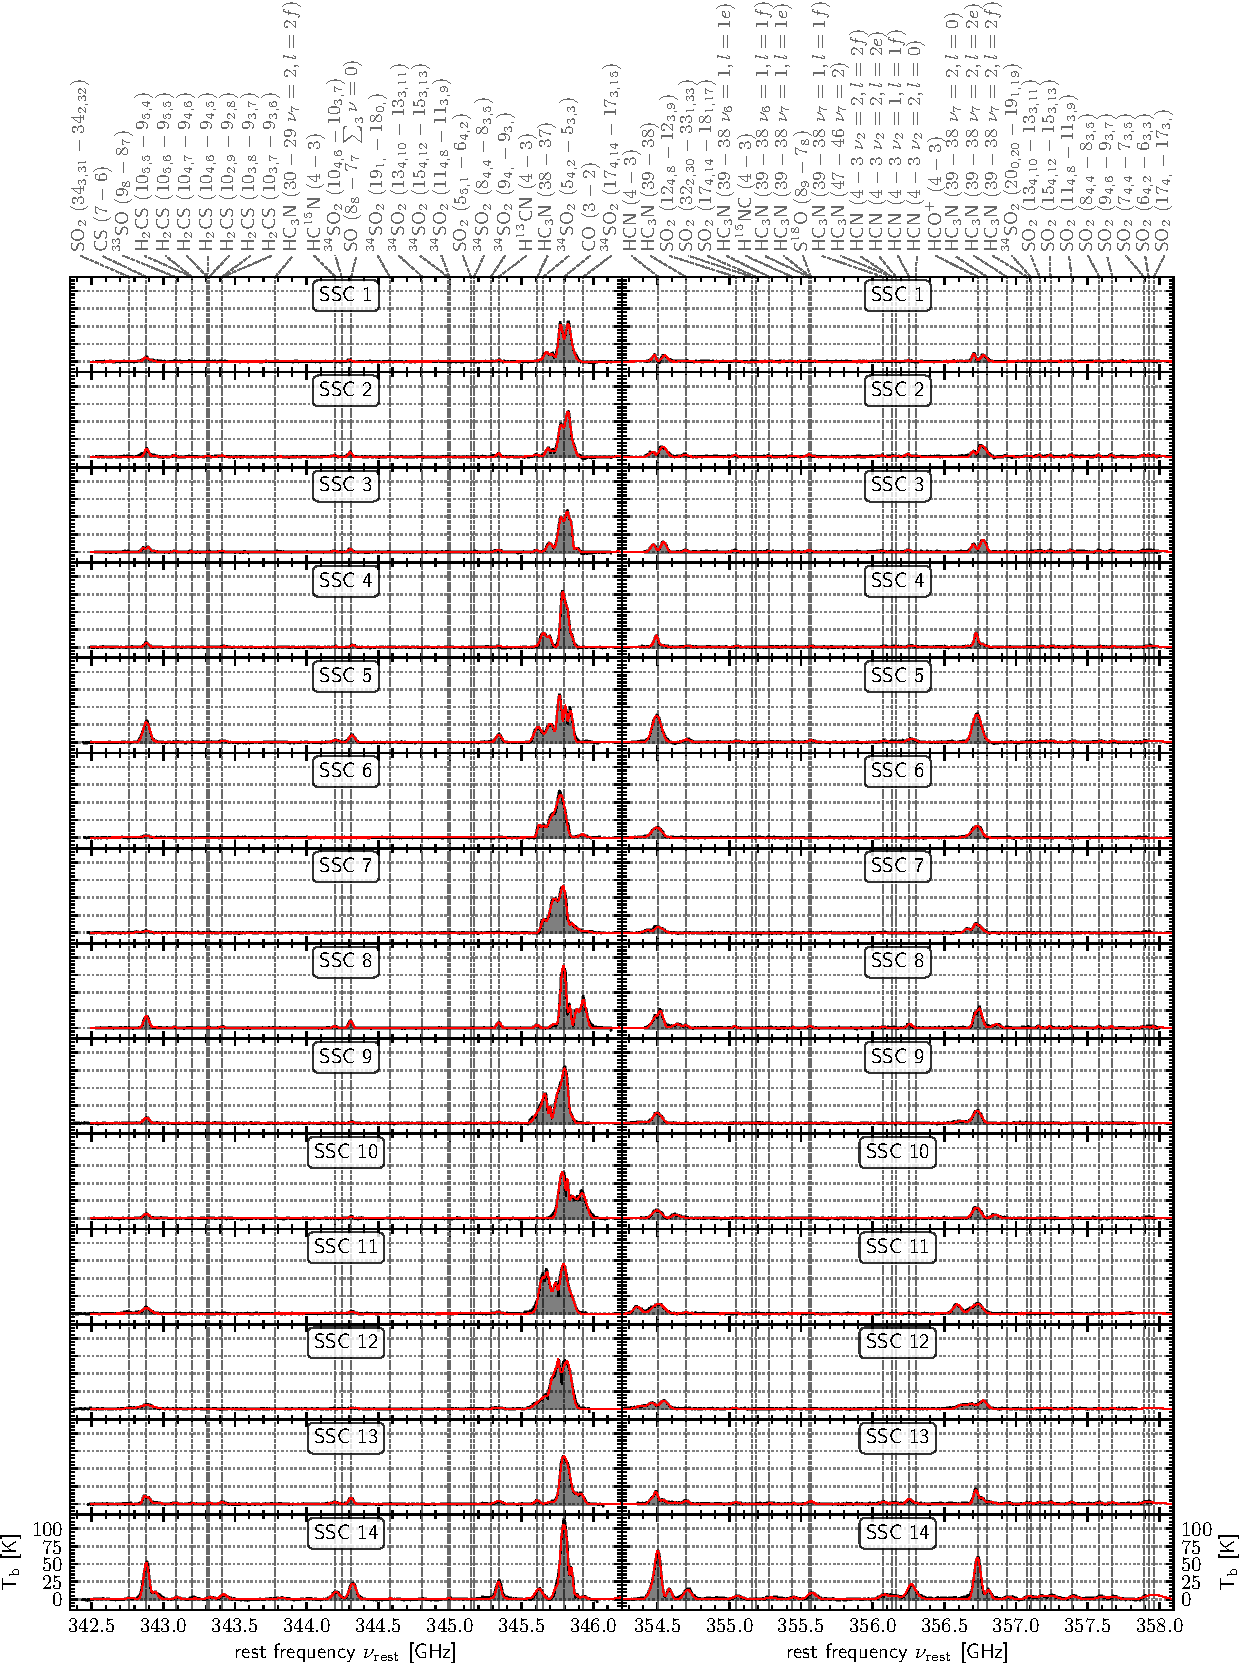
\includegraphics[width=\textwidth]{images/chapters/papers/SSCs/SSCs_all_spectra}
    \caption[Spectra on the 14 SSCs at $\sim 350$\,GHz]{Spectra (black) and \xclass fits (red) of the 14 SSCs. Note that the frequency axis is presented as rest frequency to allow for easier interpretation of the spectra (cf. Section~\ref{SSCs: section: spectra}). The detected species are labeled at the top. A zoom-in of this figure is given in Figure~\ref{SSCs: figure: sample spectrum} for SSC~14.}
    \label{SSCs: figure: fitted bands}
\end{figure*}

% sample figure from the figure set
\begin{figure*}
    \centering
    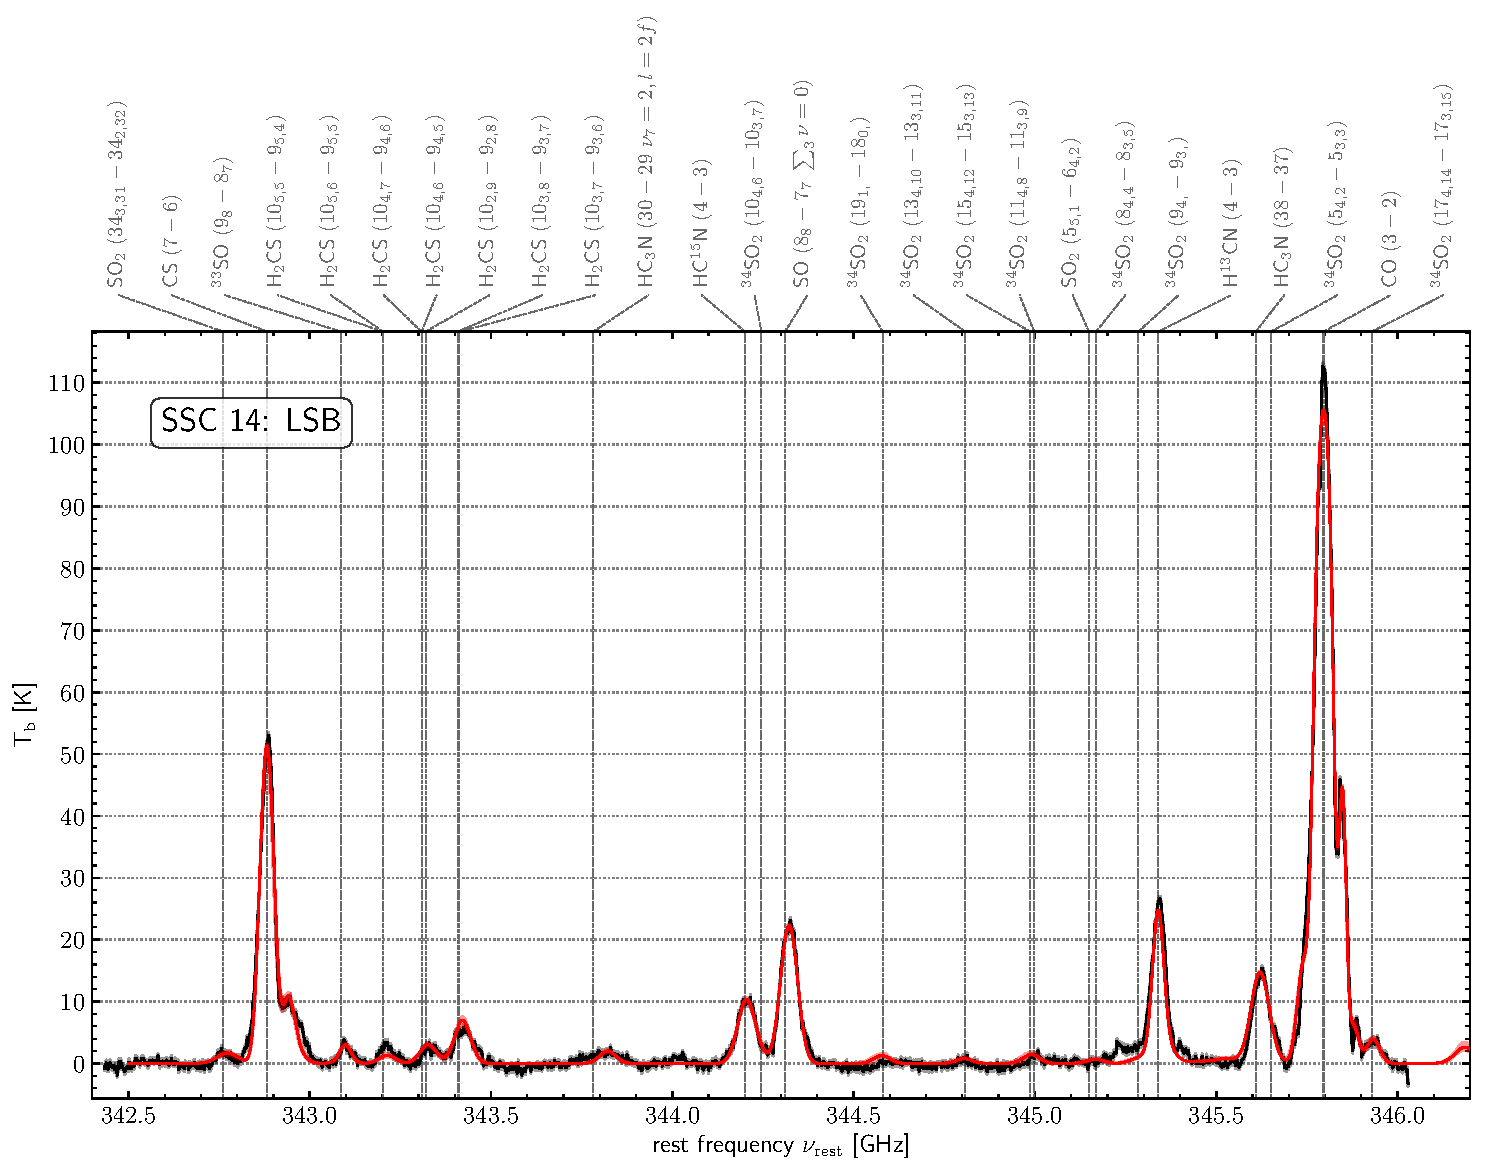
\includegraphics[height=0.4\textheight]{images/chapters/papers/SSCs/SSC_14.LSB.spectrum.pdf}
    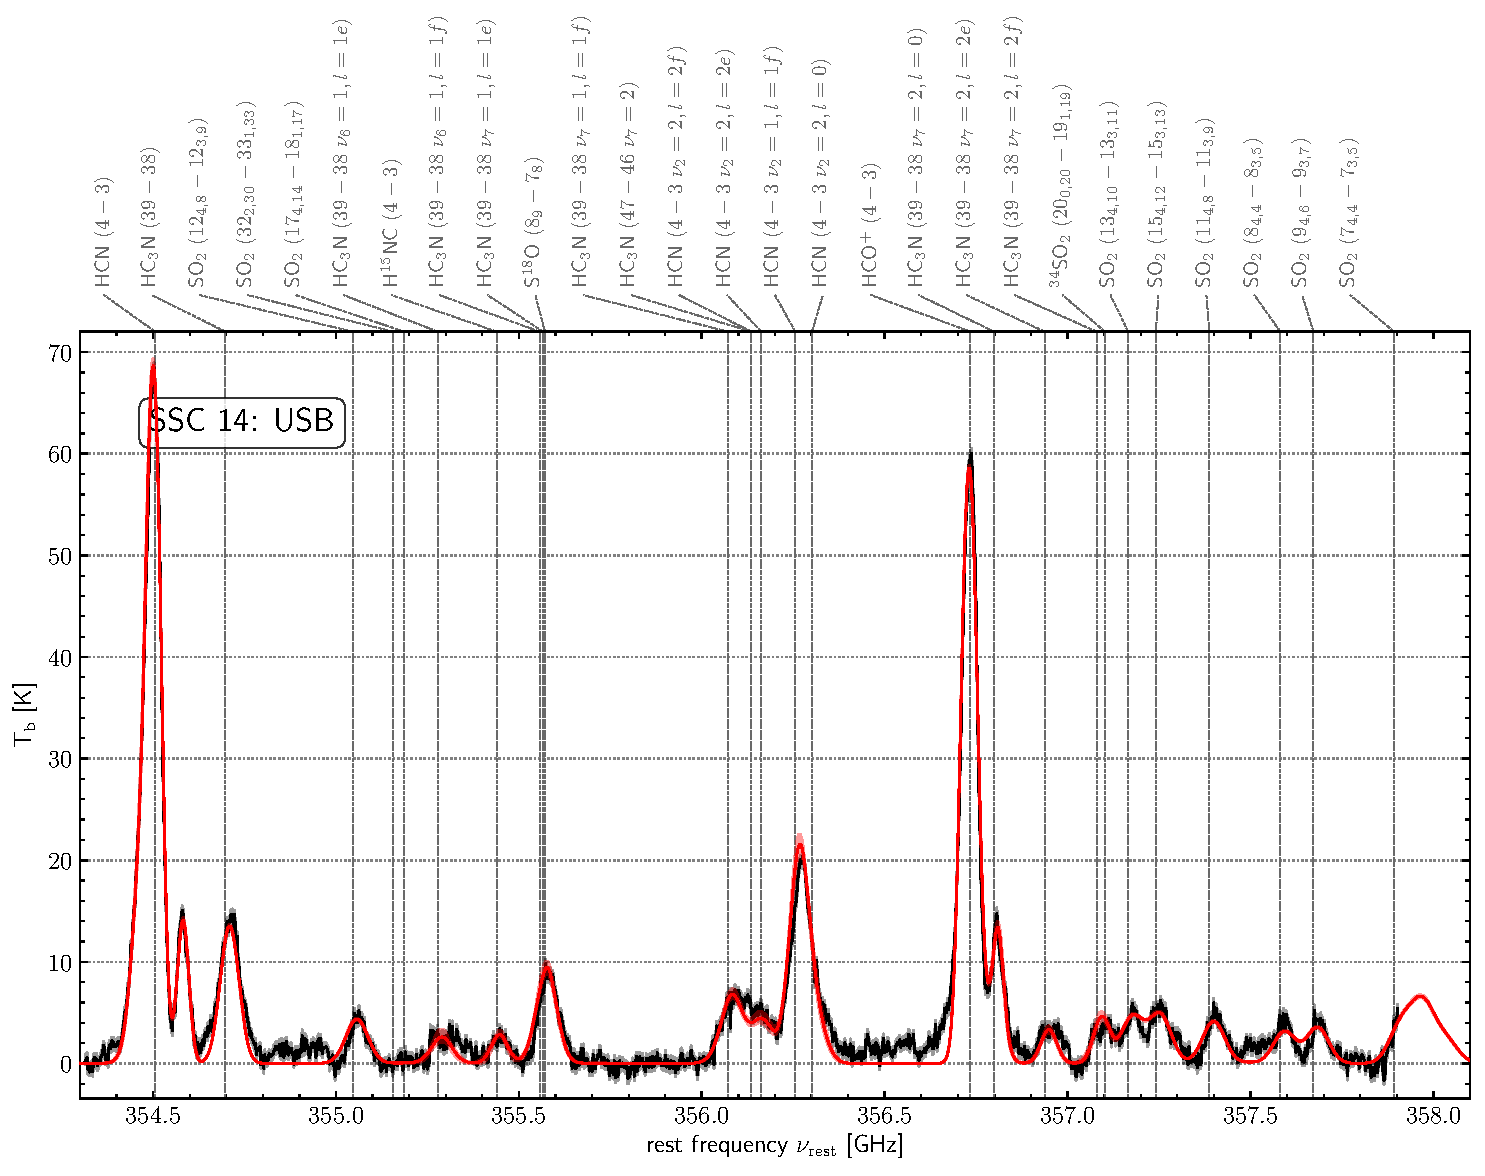
\includegraphics[height=0.4\textheight]{images/chapters/papers/SSCs/SSC_14.USB.spectrum.pdf}
    \caption[Spectra of SSC~14]{Spectra of SSC~14 in the LSB (\emph{top}) and USB (\emph{bottom}). These plots show a zoom into the bottom two panels of Figure~\ref{SSCs: figure: fitted bands}. The observed spectrum (black) sits on top of a grey band indicating the $16^\mathrm{th}$ to $84^\mathrm{th}$ percentiles of the noise added for error estimation in the fit (cf. Section~\ref{SSCs: section: error estimation}). The red lines represent the median fit obtained by \xclass using the fitting procedure described in Section~\ref{SSCs: section: spectral fitting procedure}. The Monte Carlo-estimated errors are shown as a red band ($16^\mathrm{th}$ to $84^\mathrm{th}$ percentiles) that is hardly visible due to its small size relative to the strong spectral lines. 
    The complete figure set of 14 images is available in the online journal. The spectra are available in electronic form as the Data behind the Figure.}
    \label{SSCs: figure: sample spectrum}
\end{figure*}


%%%%%%%%%%%%%%%%%%%%%%%%%%%%%%%%%%%%%%%%%%%%%%%%%%%%%%%%%%%%%%%%%%%%%%%%%%%%%%%%%%%%%%%%%%%%%%%%%%%%

\section{Spectral Line Fitting with \xclass}\label{SSCs: section: spectral line fitting}

As lines of the same or different species are blended in the spectra, an integration over a line over a fixed velocity range will overestimate the actual intensity of the line. We therefore optimize model spectra to the observed spectra using the eXtended CASA Line Analysis Software Suite \citep[\xclass\footnote{\url{https://xclass.astro.uni-koeln.de/Home}},][]{2018ascl.soft10016M}. This method requires some physical assumptions about the emission but yields a physical interpretation of the spectra, for instance column density or excitation temperature. It further allows us to de-blend the spectra and unambiguously derive observational properties such as integrated intensity.
Table~\ref{SSCs: table: intensities} lists the 55 lines that we fit for.

\subsection{Treatment of multiple spectral components}
The \co32, \hcn, \hco and \cs lines show multiple peaks of varying strength in the spectra whereas all other lines do not show noticeable deviations from Gaussian shapes within noise limits. From the line profiles alone it is impossible to decide if a double peak seen in a line is the result of multiple emission components or absorption. For consistency, we assume that the spectra are composed of emission components only and try to model them with as few components as necessary. In \co32, five or six components are required while in \hcn, \hco and \cs up to three components suffice to achieve a good fit. Upon closer inspection of the fit results below, it seems likely that the appearance of multiple components in a few cases is at least partially caused by absorption.
In the following, ``main component'' denotes the velocity component closest to the source's systemic velocity (as defined by the brightest \cs peak and consistent with the single component species, cf. Section~\ref{SSCs: section: spectra}) which is usually also the brightest component.


\subsection{Spectral fitting procedure}
\label{SSCs: section: spectral fitting procedure}

The observed spectral lines originate from (rotationally or vibrationally) excited molecular gas with excitation temperature $\mathrm{T}_\mathrm{ex}$ and column density N. The dependence of observed line amplitude, width and shape on $\mathrm{T}_\mathrm{ex}$ and N is complex and requires solving the radiative transfer. This task is simplified substantially by software tools and the availability of cataloged line properties. In this work, we use \xclass for this task. \xclass models input data by solving the radiative transfer equation for an isothermal object in one dimension and optimizes the model using the \textsc{MAGIX} optimizer to fit the data.
The molecular parameters required for this task are obtained from the CDMS catalog.

The complexity of fitting up to 55 lines with $n \times 55$ parameters is challenging and cannot reliably be done in one go. We instead employ a three step method to obtain the best possible results: (1) an unconstrained, independent \xclass fit of each species individually for each source, followed by (2) a joint fit of all detected species to the whole data range for each source, and (3) refinement fits for selected species while keeping all other species fixed.

In the first run, we fit the species completely independently or include in the fit as few other lines as possible. This allows us to explore a large parameter range with a simple fit. 
A joint fit a of whole band is much more complicated due to the many, often blended, lines in each band and only succeeds if the parameter range is limited sufficiently by the first run. We restrict the fit parameters in the second run to the $16^\mathrm{th} - 84^\mathrm{th}$ percentile range of the respective parameter of the first run.
In the third run, we fit for the excitation temperature of the temperature sensitive species while keeping all other species fixed. 
This approach limits the degrees of freedom in each run to a manageable level. 

The parameters we fit for are column density, linewidth and line centroid. We fix the source size to unity which means the source completely covers the beam, a reasonable estimate for slightly unresolved SSCs \Leroy{p}. The species in our sample are typically detected with only a single line, so we have to assume an excitation temperature or infer it from the data. The latter cannot be done for all SSCs (see discussion in section \ref{SSCs: section: ISM temperature}), so we fix $\mathrm{T_{rot}}=130$\,K for the purely rotationally excited species and $\mathrm{T_{vib}}=300$\,K for the ro-vibrational transitions. The former corresponds to the warm ISM component found by \citet{2013ApJ...779...33M} and \citet{Gorski:2017es} on lower spatial resolution. Using this value, our analysis is consistent with \Leroy{t}, who used the same value. As it turns out (Section~\ref{SSCs: section: ISM temperature}), the mean rotational temperature of the SSCs where this measurement is possible is 127\,K, hence $\mathrm{T_{rot}}=130$\,K is a good assumption. 
The assumption of $\mathrm{T_{vib}}=300$\,K is an educated guess and supposedly on the lower side for an SSC environment \citep[compared to less extreme Galactic hot cores as in][]{1983ApJ...274..184G,1999A&A...341..882W}.

In the third run, we fit SO$_2$ and H$_2$CS for the most unstable parameter, the excitation temperature $\mathrm{T_{rot}}$, in the range $25-1000$\,K. Other species than these two do not cover enough range in the energy states or detected lines for successful fits with free temperature parameters.

For our XCLASS fits, we find that an under-/overestimation in the fixed excitation temperature causes over-/underestimation in column density by similar factors. Fitted column densities must thus be understood with a systematic error of the same order than the assumed excitation temperature (see discussion in Section~\ref{SSCs: section: ISM temperature}). 
For column density ratios of two species, this systematic effect affects both species equally if the excitation temperature is equally under-/overestimated. In practise, the excitation temperatures are not identical but should be similar for two considered species, so their column density ratio is only weakly affected.

\subsection{Error estimation}
\label{SSCs: section: error estimation}

We estimate fit errors with a Monte Carlo scheme with 100 variations of the spectra to fit. For each variation, we add random draws of Gaussian noise to the observed spectra and thus sample the fit robustness against noise in the spectra which is the dominant source of error.
%We repeat each \xclass fit 100 times with spectra varied within the noise to sample the fit robustness against noise in the spectra. 
Errors are reported as the differences between median and $16^\mathrm{th}$ ($84^\mathrm{th}$) percentiles\footnote{For Gaussian distributions, this range corresponds to $\pm1\sigma$.} for lower (upper) error.

Details regarding the handling of blended lines, parameters and parameter ranges (especially a discussion of the choice of $\mathrm{T_{ex}}$ and its implications), fit algorithms and the Monte Carlo error estimation are described in Appendix~\ref{appendix: SSCs: xclass}.

\subsection{Derivation of integrated intensity}
\xclass does not offer the possibility to also report integrated intensity since it is built on physical instead of observational quantities. We therefore use the final \xclass models to de-blend the spectra and derive integrated intensities for lines within the observed frequency range of the fitted species. This is done through Gaussian fits to the de-blended spectra. As such the integrated intensities inherit uncertainties due to blended lines and the Monte Carlo error estimation from the \xclass fits.


\subsection{Fitted spectra}\label{SSCs: section: fitted spectra}

The observed spectra with the joint fit (third run) for all 14 SSCs in both sidebands are shown in Figure~\ref{SSCs: figure: fitted bands}. Figure~\ref{SSCs: figure: sample spectrum} provides an enlarged view of the spectra for SSC~14. 
The corresponding enlarged spectra for SSCs~1-13 can be found in Figure Set 2 in the online journal.
In general, the model spectra fit the observed data well with only small deviations. Spectral ranges with many blended lines are less well fit than isolated bright lines but the fit reliably disentangles the relative contribution of the species. 
The fit can deviate from the data slightly because \xclass fits all lines of a species simultaneously and respects the relations between lines. A particular line may thus be under-/overestimated if another line of the same species is found at lower/higher relative intensity. 
Some spectra, especially of the bright sources like SSC~14, show more spectral features than fitted, which will be studied in future work.
The fits prove to provide robust parameter estimates as indicated by the Monte Carlo error estimation. Noise fluctuation and repetition of the fit only marginably affect the results. Hence, the dominant source of error is the flux calibration and continuum subtraction (only relevant in the USB for SSCs~2, 3, 4, 8, 13, 14). Note that
the LTE approximation used by \xclass is also a severe source of uncertainty if the conditions in the SSCs are not close to LTE conditions.


%%%%%%%%%%%%%%%%%%%%%%%%%%%%%%%%%%%%%%%%%%%%%%%%%%%%%%%%%%%%%%%%%%%%%%%%%%%%%%%%%%%%%%%%%%%%%%%%%%%%
% intensity table
%%%%%%%%%%%%%%%%%%%%%%%%%%%%%%%%%%%%%%%%%%%%%%%%%%%%%%%%%%%%%%%%%%%%%%%%%%%%%%%%%%%%%%%%%%%%%%%%%%%%

\begin{sidewaystable}[ph]
\begin{threeparttable}
    \centering
    \footnotesize
    \caption[Fitted line intensities]{Sample of the fitted integrated intensities in K\,\kms. The full table is available in the machine-readable format including error intervals. The shown sample of the strongest spectral lines provides guidance regarding its form and content.
    \label{SSCs: table: intensities}}
    
    \begin{tabular}{lclcrrrrrrrrrrrrrr}
        \toprule
        molecule & \multicolumn{2}{c}{transition} & comp.$^\dagger$ & \multicolumn{14}{c}{SSC no.}\\ \cline{2-3} \cline{5-18}
        & rotational & vibrational & & 1 & 2 & 3 & 4 & 5 & 6 & 7 & 8 & 9 & 10 & 11 & 12 & 13 & 14\\
        \midrule
CO             & 3--2                     & $\nu=0$         & 0 &  810 &  684 &  167 &  744 & 1607 &  199 &  149 & 1361 &  188 & 3004 & 1451 & 4132 &  161 &  127 \\
CO             & 3--2                     & $\nu=0$         & 1 & 1741 & 2328 & 1692 &  788 & 1014 & 3509 &  249 &  394 & 2919 &  418 & 2978 & 2962 & 3552 &  197 \\
CO             & 3--2                     & $\nu=0$         & 2 & 1737 & 1698 &  568 & 2654 & 2048 & 1862 &  324 &  702 & 2308 & 1462 & 1148 & 1749 & 1114 &  806 \\
CO             & 3--2                     & $\nu=0$         & 3 &  288 &  245 & 2187 &  724 & 1452 &  302 & 2678 &  496 &  212 & 2103 &  959 &  575 &  904 & 5486 \\
CO             & 3--2                     & $\nu=0$         & 4 &  551 &  367 &  544 &  501 & 1030 &  491 & 3327 & 3578 & 1096 &  747 & 1148 &  762 &  406 &  517 \\
CO             & 3--2                     & $\nu=0$         & 5 &  ... &  ... &  ... &  ... &  ... &  ... &  572 &  232 & 1282 &  ... & 2593 &  ... &  ... &  ... \\
HCO$^+$        & 4--3                     & $\nu=0$         & 0 &  366 &  736 &  630 &  321 & 2460 &  638 &  527 &  812 &  327 &  884 &  463 &  616 &  604 &  246 \\
HCO$^+$        & 4--3                     & $\nu=0$         & 1 &  278 &  212 &  333 &  352 &  ... &  499 &  157 &  647 &  840 &  295 &  600 &  391 &  153 & 2591 \\
HCO$^+$        & 4--3                     & $\nu=0$         & 2 &  ... &  ... &  ... &   43 &  ... &  ... &  209 &  280 &  208 &  ... &  715 &  317 &  104 &  ... \\
HCN            & 4--3                     & $\nu=0$         & 0 &  354 &  727 &  547 &  234 & 2230 & 1021 &  263 &  798 &  406 &  736 &  556 &  678 &  267 &  477 \\
HCN            & 4--3                     & $\nu=0$         & 1 &  201 &  127 &  286 &  324 &  ... &  ... &  209 &  569 &  537 &  290 &  581 &  404 &  398 & 2399 \\
HCN            & 4--3                     & $\nu=0$         & 2 &  ... &  ... &  ... &  ... &  ... &  ... &  178 &  289 &  137 &  ... &  527 &  280 &  124 &  ... \\
HCN            & 4--3                     & $\nu_2=2$, l=2f & 0 &    6 &   25 &   12 &   28 &   28 &  ... &  ... &    9 &  ... &  ... &  ... &  ... &   41 &  141 \\
HCN            & 4--3                     & $\nu_2=2$, l=2e & 0 &    6 &   25 &   12 &   28 &   28 &  ... &  ... &    9 &  ... &  ... &  ... &  ... &   41 &  136 \\
HCN            & 4--3                     & $\nu_2=2$, l=0  & 0 &    9 &   36 &   17 &   40 &   39 &  ... &  ... &   13 &  ... &  ... &  ... &  ... &   59 &  197 \\
HCN            & 4--3                     & $\nu_2=1$, l=1f & 0 &   55 &  127 &   93 &   79 &  283 &  ... &  ... &  212 &  ... &  ... &   34 &  ... &  288 & 1179 \\
H$^{13}$CN     & 4--3                     & $\nu=0$         & 0 &   32 &   53 &   41 &   13 &  370 &   34 &  ... &  177 &   51 &   11 &   92 &   69 &  124 &  697 \\
HC$^{15}$N     & 4--3                     & $\nu=0$         & 0 &  ... &   61 &   52 &   22 &  167 &  ... &  ... &   76 &  ... &  ... &  ... &  ... &  130 &  534 \\
H$^{15}$NC     & 4--3                     & $\nu=0$         & 0 &   17 &   39 &   31 &  ... &   71 &  ... &  ... &   27 &  ... &  ... &  ... &  ... &   37 &  135 \\
CS             & 7--6                     & $\nu=0$         & 0 &   97 &  103 &   61 &  209 & 1452 &  118 &  126 &  654 &  337 &  238 &  498 &  551 &  282 & 2116 \\
CS             & 7--6                     & $\nu=0$         & 1 &  172 &  268 &  132 &  ... &  ... &  ... &   40 &  ... &  ... &   79 &  ... &  ... &  238 &  285 \\
CS             & 7--6                     & $\nu=0$         & 2 &  ... &  ... &  151 &  ... &  ... &  ... &  ... &  ... &  ... &  ... &  ... &  ... &   54 &  ... \\
% HC$_3$N        & 38--37                   & $\nu=0$         & 0 &   57 &  132 &   70 &   85 &  225 &  ... &  ... &  132 &  ... &   55 &   99 &  ... &  187 &  790 \\
% HC$_3$N        & 39--38                   & $\nu=0$         & 0 &   53 &  122 &   65 &   79 &  208 &  ... &  ... &  122 &  ... &   51 &   91 &  ... &  173 &  733 \\
% HC$_3$N        & 39--38                   & $\nu_6=1$, l=1e & 0 &    8 &   29 &   35 &   11 &   46 &  ... &  ... &   18 &  ... &  ... &  ... &  ... &   55 &  156 \\
% HC$_3$N        & 39--38                   & $\nu_6=1$, l=1f & 0 &    8 &   29 &   35 &   11 &   46 &  ... &  ... &   18 &  ... &  ... &  ... &  ... &   55 &  156 \\
% HC$_3$N        & 39--38                   & $\nu_7=1$, l=1e & 0 &  ... &   73 &   56 &   26 &   93 &  ... &  ... &   56 &  ... &  ... &   15 &  ... &  123 &  379 \\
% HC$_3$N        & 39--38                   & $\nu_7=1$, l=1f & 0 &  ... &   73 &   56 &   26 &   93 &  ... &  ... &   56 &  ... &  ... &   15 &  ... &  123 &  379 \\
% HC$_3$N        & 39--38                   & $\nu_7=2$, l=0  & 0 &  ... &   59 &   21 &   26 &   42 &  ... &  ... &  ... &  ... &  ... &  ... &  ... &   79 &  154 \\
% HC$_3$N        & 39--38                   & $\nu_7=2$, l=2e & 0 &  ... &   58 &   21 &   26 &   42 &  ... &  ... &  ... &  ... &  ... &  ... &  ... &   78 &  152 \\
% HC$_3$N        & 39--38                   & $\nu_7=2$, l=2f & 0 &  ... &   58 &   21 &   26 &   42 &  ... &  ... &  ... &  ... &  ... &  ... &  ... &   78 &  152 \\
% SO             & 8$_{8}$--7$_{7}$         & $\nu=0$         & 0 &   58 &  157 &  115 &   86 &  431 &  ... &  ... &  291 &   62 &   80 &  115 &   56 &  286 & 1135 \\
% $^{33}$SO      & 9$_{8}$--8$_{7}$         & $\nu=0$         & 0 &  ... &   44 &   35 &  ... &  ... &  ... &  ... &   27 &  ... &  ... &  ... &  ... &   44 &   99 \\
% S$^{18}$O      & 8$_{9}$--7$_{8}$         & $\nu=0$         & 0 &   35 &   11 &  ... &   10 &    6 &  ... &  ... &   18 &  ... &  ... &  ... &  ... &  ... &   12 \\
% SO$_2$         & 34$_{3,31}$--34$_{2,32}$ & $\nu=0$         & 0 &  ... &    3 &    1 &   16 &    9 &  ... &  ... &    5 &  ... &  ... &    2 &   46 &    7 &  107 \\
% SO$_2$         & 5$_{5,1}$--6$_{4,2}$     & $\nu=0$         & 0 &  ... &    1 &    2 &    1 &    2 &  ... &  ... &    1 &  ... &  ... &  ... &  ... &    2 &    5 \\
% SO$_2$         & 12$_{4,8}$--12$_{3,9}$   & $\nu=0$         & 0 &   34 &   69 &   79 &   63 &   99 &  ... &  ... &   59 &  ... &   24 &   19 &   39 &  113 &  279 \\
% SO$_2$         & 13$_{4,10}$--13$_{3,11}$ & $\nu=0$         & 0 &   32 &   69 &   77 &   65 &  103 &  ... &  ... &   60 &  ... &   21 &   19 &   42 &  114 &  293 \\
% SO$_2$         & 15$_{4,12}$--15$_{3,13}$ & $\nu=0$         & 0 &   28 &   65 &   68 &   67 &   99 &  ... &  ... &   58 &  ... &   15 &   18 &   47 &  109 &  306 \\
% SO$_2$         & 11$_{4,8}$--11$_{3,9}$   & $\nu=0$         & 0 &   35 &   69 &   80 &   61 &   99 &  ... &  ... &   59 &  ... &   27 &   19 &   36 &  112 &  264 \\
% SO$_2$         & 8$_{4,4}$--8$_{3,5}$     & $\nu=0$         & 0 &   32 &   59 &   72 &   47 &   82 &  ... &  ... &   49 &  ... &   31 &   15 &   26 &   94 &  208 \\
% SO$_2$         & 9$_{4,6}$--9$_{3,7}$     & $\nu=0$         & 0 &   34 &   64 &   77 &   53 &   90 &  ... &  ... &   53 &  ... &   30 &   17 &   30 &  103 &  224 \\
% SO$_2$         & 7$_{4,4}$--7$_{3,5}$     & $\nu=0$         & 0 &   31 &   53 &   76 &   35 &   83 &  ... &  ... &   43 &  ... &   23 &   47 &   51 &   78 &  134 \\
% SO$_2$         & 6$_{4,2}$--6$_{3,3}$     & $\nu=0$         & 0 &   46 &   42 &  102 &   50 &   77 &  ... &  ... &   34 &  ... &   37 &   49 &   54 &   41 &  143 \\
% SO$_2$         & 17$_{4,}$--17$_{3,}$     & $\nu=0$         & 0 &   20 &   59 &   31 &   54 &   83 &  ... &  ... &   55 &  ... &   30 &   49 &   46 &  187 &  456 \\
% $^{34}$SO$_2$  & 10$_{4,6}$--10$_{3,7}$   & $\nu=0$         & 0 &  ... &  ... &  ... &  ... &  ... &  ... &  ... &  ... &  ... &  ... &  ... &  ... &  ... &   35 \\
% $^{34}$SO$_2$  & 20$_{0,20}$--19$_{1,19}$ & $\nu=0$         & 0 &  ... &  ... &  ... &  ... &  ... &  ... &  ... &  ... &  ... &  ... &  ... &  ... &  ... &   60 \\
% $^{34}$SO$_2$  & 19$_{1,}$--18$_{0,}$     & $\nu=0$         & 0 &  ... &  ... &  ... &  ... &  ... &  ... &  ... &  ... &  ... &  ... &  ... &  ... &  ... &   62 \\
% $^{34}$SO$_2$  & 13$_{4,10}$--13$_{3,11}$ & $\nu=0$         & 0 &  ... &  ... &  ... &  ... &  ... &  ... &  ... &  ... &  ... &  ... &  ... &  ... &  ... &   37 \\
% $^{34}$SO$_2$  & 15$_{4,12}$--15$_{3,13}$ & $\nu=0$         & 0 &  ... &  ... &  ... &  ... &  ... &  ... &  ... &  ... &  ... &  ... &  ... &  ... &  ... &   36 \\
% $^{34}$SO$_2$  & 11$_{4,8}$--11$_{3,9}$   & $\nu=0$         & 0 &  ... &  ... &  ... &  ... &  ... &  ... &  ... &  ... &  ... &  ... &  ... &  ... &  ... &   36 \\
% $^{34}$SO$_2$  & 8$_{4,4}$--8$_{3,5}$     & $\nu=0$         & 0 &  ... &  ... &  ... &  ... &  ... &  ... &  ... &  ... &  ... &  ... &  ... &  ... &  ... &   30 \\
% $^{34}$SO$_2$  & 9$_{4,}$--9$_{3,}$       & $\nu=0$         & 0 &  ... &  ... &  ... &  ... &  ... &  ... &  ... &  ... &  ... &  ... &  ... &  ... &  ... &   33 \\
% $^{34}$SO$_2$  & 5$_{4,2}$--5$_{3,3}$     & $\nu=0$         & 0 &  ... &  ... &  ... &  ... &  ... &  ... &  ... &  ... &  ... &  ... &  ... &  ... &  ... &   50 \\
% $^{34}$SO$_2$  & 17$_{4,14}$--17$_{3,15}$ & $\nu=0$         & 0 &  ... &  ... &  ... &  ... &  ... &  ... &  ... &  ... &  ... &  ... &  ... &  ... &  ... &   33 \\
% H$_2$CS        & 10$_{5,5}$--9$_{5,4}$    & $\nu=0$         & 0 &  ... &    4 &   12 &   13 &   36 &  ... &  ... &   13 &  ... &  ... &  ... &  ... &   21 &   40 \\
% H$_2$CS        & 10$_{5,6}$--9$_{5,5}$    & $\nu=0$         & 0 &  ... &    5 &   12 &   14 &   37 &  ... &  ... &   14 &  ... &  ... &  ... &  ... &   23 &   40 \\
% H$_2$CS        & 10$_{4,7}$--9$_{4,6}$    & $\nu=0$         & 0 &  ... &  ... &   18 &   23 &   47 &  ... &  ... &   15 &  ... &  ... &  ... &  ... &   42 &   75 \\
% H$_2$CS        & 10$_{4,6}$--9$_{4,5}$    & $\nu=0$         & 0 &  ... &  ... &  ... &   17 &   39 &  ... &  ... &   20 &  ... &  ... &  ... &  ... &   22 &   75 \\
% H$_2$CS        & 10$_{2,9}$--9$_{2,8}$    & $\nu=0$         & 0 &  ... &   57 &   24 &  ... &  101 &  ... &  ... &   60 &  ... &  ... &  ... &  ... &   98 &   19 \\
% H$_2$CS        & 10$_{3,8}$--9$_{3,7}$    & $\nu=0$         & 0 &  ... &  ... &   24 &   26 &  ... &  ... &  ... &  ... &  ... &  ... &  ... &  ... &  ... &  150 \\
% H$_2$CS        & 10$_{3,7}$--9$_{3,6}$    & $\nu=0$         & 0 &  ... &   30 &   23 &   43 &   45 &  ... &  ... &   30 &  ... &  ... &  ... &  ... &   18 &  177 \\
        \bottomrule
    \end{tabular}
    \tablenote{The typical intensity error is 13.0\% and consists primarily of uncertainty due to line crowding. Additionally, the systematic flux uncertainty applies with $\LESSSIM 5\%$ for these observations according to the ALMA specifications.\\
    $\dagger$ Components do not necessarily correspond to each other. For instance, the undetected marks (...) for component 5 of \co32 in SSC~1 merely indicate that five components fit the spectrum sufficiently well whereas in SSC~7 six components are required.
    }
\end{threeparttable}
\end{sidewaystable}


%%%%%%%%%%%%%%%%%%%%%%%%%%%%%%%%%%%%%%%%%%%%%%%%%%%%%%%%%%%%%%%%%%%%%%%%%%%%%%%%%%%%%%%%%%%%%%%%%%%%
% fit table
%%%%%%%%%%%%%%%%%%%%%%%%%%%%%%%%%%%%%%%%%%%%%%%%%%%%%%%%%%%%%%%%%%%%%%%%%%%%%%%%%%%%%%%%%%%%%%%%%%%%

\begin{table}[ph]
    \centering
    \begin{threeparttable}
        \caption[Fitted species parameters]{Sample of the parameters fitted with XCLASS. The full table is available in the machine-readable format including error intervals. The shown sample for SSC~1 provides guidance regarding its form and content.
        \label{SSCs: table: column densities}}

        \begin{tabular}{rlcccrrrrr}
            \toprule
            SSC & molecule & vibration & component & $\log \mathrm{N}$ & $\sigma$ & $\mu$ & T$_\mathrm{kin}$ & $\tau_\mathrm{int}$ \\
            & & & & [\pcm2] & [\kms] & [\kms] & [K] & \\
            & & & (1) & (2) & (3) & (4) & (5) & (6) \\
            \midrule
1 & CO           & $\nu=0$      & 0 & 17.85 & 40.0 &  -44.6 & 130 &  3.32 \\
1 & CO           & $\nu=0$      & 1 & 18.23 & 33.3 &  -22.1 & 130 &  7.89 \\
1 & CO           & $\nu=0$      & 2 & 18.24 & 29.0 &   20.3 & 130 &  8.08 \\
1 & CO           & $\nu=0$      & 3 & 17.39 & 30.0 &   68.7 & 130 &  1.15 \\
1 & CO           & $\nu=0$      & 4 & 17.68 & 39.6 &  106.2 & 130 &  2.22 \\
1 & HCO$^+$      & $\nu=0$      & 0 & 14.40 & 39.4 &  -34.3 & 130 &  1.50 \\
1 & HCO$^+$      & $\nu=0$      & 1 & 14.28 & 22.7 &   24.2 & 130 &  1.15 \\
1 & HCN          & $\nu=0$      & 0 & 14.62 & 37.4 &  -37.1 & 130 &  1.44 \\
1 & HCN          & $\nu=0$      & 1 & 14.38 & 20.5 &   24.6 & 130 &  0.82 \\
1 & HCN          & $\nu_2=2$    & 0 & 16.29 & 31.9 &   -5.3 & 300 &  0.04 \\
1 & HCN          & $\nu_2=1$    & 0 & 15.64 & 30.5 &    7.5 & 300 &  0.18 \\
1 & H$^{13}$CN   & $\nu=0$      & 0 & 13.59 & 20.3 &   -3.9 & 130 &  0.13 \\
1 & H$^{15}$NC   & $\nu=0$      & 0 & 13.37 & 18.1 &   10.0 & 130 &  0.07 \\
1 & CS           & $\nu=0$      & 0 & 14.53 & 33.9 &  -21.7 & 130 &  0.38 \\
1 & CS           & $\nu=0$      & 1 & 14.78 & 32.7 &    3.3 & 130 &  0.67 \\
1 & HC$_3$N      & $\nu=0$      & 0 & 14.66 & 50.0 &   -0.3 & 130 &  0.43 \\
1 & HC$_3$N      & $\nu_6=1$    & 0 & 14.95 & 26.5 &   -0.7 & 300 &  0.05 \\
1 & SO           & $\nu=0$      & 0 & 15.04 & 21.6 &    8.8 & 130 &  0.51 \\
1 & S$^{18}$O    & $\nu=0$      & 0 & 14.85 & 48.6 &    9.9 & 130 &  0.14 \\
1 & SO$_2$       & $\nu=0$      & 0 & 15.52 & 35.1 &    1.9 &  84 &  3.53 \\
% 2 & CO           & $\nu=0$      & 0 & 17.78 & 34.3 &  -44.6 & 130 &  2.80 \\
% 2 & CO           & $\nu=0$      & 1 & 18.37 & 33.5 &  -22.5 & 130 & 10.81 \\
% 2 & CO           & $\nu=0$      & 2 & 18.21 & 34.4 &   18.9 & 130 &  7.64 \\
% 2 & CO           & $\nu=0$      & 3 & 17.32 & 29.9 &   65.9 & 130 &  0.97 \\
% 2 & CO           & $\nu=0$      & 4 & 17.50 & 29.0 &   98.8 & 130 &  1.47 \\
% 2 & HCO$^+$      & $\nu=0$      & 0 & 14.71 & 46.3 &  -26.7 & 130 &  3.08 \\
% 2 & HCO$^+$      & $\nu=0$      & 1 & 14.16 & 25.9 &   29.3 & 130 &  0.87 \\
% 2 & HCN          & $\nu=0$      & 0 & 14.94 & 46.4 &  -26.7 & 130 &  3.02 \\
% 2 & HCN          & $\nu=0$      & 1 & 14.17 & 22.5 &   30.3 & 130 &  0.51 \\
% 2 & HCN          & $\nu_2=2$    & 0 & 16.89 & 28.7 &   -6.4 & 300 &  0.14 \\
% 2 & HCN          & $\nu_2=1$    & 0 & 16.00 & 31.2 &    9.9 & 300 &  0.42 \\
% 2 & H$^{13}$CN   & $\nu=0$      & 0 & 13.81 & 13.7 &   -3.7 & 130 &  0.21 \\
% 2 & HC$^{15}$N   & $\nu=0$      & 0 & 13.87 & 29.7 &    8.8 & 130 &  0.24 \\
% 2 & HC$_3$N      & $\nu=0$      & 0 & 15.03 & 41.8 &    5.8 & 130 &  1.01 \\
% 2 & HC$_3$N      & $\nu_6=1$    & 0 & 15.50 & 20.9 &    2.0 & 300 &  0.19 \\
% 2 & HC$_3$N      & $\nu_7=1$    & 0 & 15.33 & 39.3 &    7.4 & 300 &  0.48 \\
% 2 & HC$_3$N      & $\nu_7=2$    & 0 & 15.70 & 35.0 &   -1.4 & 300 &  0.58 \\
% 2 & H$^{15}$NC   & $\nu=0$      & 0 & 13.74 & 38.5 &    8.3 & 130 &  0.16 \\
% 2 & CS           & $\nu=0$      & 0 & 14.55 & 20.5 &   -2.1 & 130 &  0.40 \\
% 2 & CS           & $\nu=0$      & 1 & 14.97 & 30.7 &   -1.9 & 130 &  1.05 \\
% 2 & $^{33}$SO    & $\nu=0$      & 0 & 14.84 & 20.0 &   10.0 & 130 &  0.17 \\
% 2 & S$^{18}$O    & $\nu=0$      & 0 & 14.35 & 59.8 &   -9.7 & 130 &  0.04 \\
% 2 & SO$_2$       & $\nu=0$      & 0 & 15.88 & 20.1 &    6.0 & 114 &  5.36 \\
% 2 & H$_2$CS      & $\nu=0$      & 0 & 15.33 & 29.2 &    3.9 & 103 &  1.37 \\
% 2 & SO           & $\nu=0$      & 0 & 15.48 & 23.6 &    5.4 & 130 &  1.40 \\
% 3 & CO           & $\nu=0$      & 0 & 17.15 & 28.4 &  -75.9 & 130 &  0.66 \\
% 3 & CO           & $\nu=0$      & 1 & 18.23 & 27.5 &  -21.5 & 130 &  7.92 \\
% 3 & CO           & $\nu=0$      & 2 & 17.72 & 16.8 &  -44.4 & 130 &  2.43 \\
% 3 & CO           & $\nu=0$      & 3 & 18.33 & 38.8 &   17.2 & 130 & 10.04 \\
% 3 & CO           & $\nu=0$      & 4 & 17.67 & 39.5 &   86.3 & 130 &  2.19 \\
% 3 & HCO$^+$      & $\nu=0$      & 0 & 14.65 & 35.3 &  -31.2 & 130 &  2.65 \\
% 3 & HCO$^+$      & $\nu=0$      & 1 & 14.36 & 29.2 &   26.6 & 130 &  1.38 \\
% 3 & HCN          & $\nu=0$      & 0 & 14.82 & 35.6 &  -30.3 & 130 &  2.27 \\
% 3 & HCN          & $\nu=0$      & 1 & 14.53 & 27.8 &   28.4 & 130 &  1.17 \\
% 3 & HCN          & $\nu_2=2$    & 0 & 16.57 & 22.6 &    0.8 & 300 &  0.07 \\
% 3 & HCN          & $\nu_2=1$    & 0 & 15.87 & 27.6 &    7.1 & 300 &  0.31 \\
% 3 & H$^{13}$CN   & $\nu=0$      & 0 & 13.70 & 40.0 &   -2.5 & 130 &  0.16 \\
% 3 & HC$^{15}$N   & $\nu=0$      & 0 & 13.80 & 33.1 &    9.6 & 130 &  0.20 \\
% 3 & HC$_3$N      & $\nu=0$      & 0 & 14.76 & 25.9 &    4.4 & 130 &  0.54 \\
% 3 & HC$_3$N      & $\nu_6=1$    & 0 & 15.58 & 29.1 &    1.3 & 300 &  0.23 \\
% 3 & HC$_3$N      & $\nu_7=1$    & 0 & 15.21 & 37.1 &    7.9 & 300 &  0.37 \\
% 3 & HC$_3$N      & $\nu_7=2$    & 0 & 15.26 & 22.0 &    3.3 & 300 &  0.21 \\
% 3 & H$^{15}$NC   & $\nu=0$      & 0 & 13.64 & 25.5 &   -4.6 & 130 &  0.12 \\
% 3 & CS           & $\nu=0$      & 0 & 14.32 & 31.3 &  -25.1 & 130 &  0.23 \\
% 3 & CS           & $\nu=0$      & 1 & 14.66 & 19.6 &   -9.9 & 130 &  0.51 \\
% 3 & CS           & $\nu=0$      & 2 & 14.72 & 24.7 &   18.7 & 130 &  0.59 \\
% 3 & $^{33}$SO    & $\nu=0$      & 0 & 14.74 & 22.8 &    7.5 & 130 &  0.13 \\
% 3 & S$^{18}$O    & $\nu=0$      & 0 & 12.28 & 29.5 &   -9.4 & 130 &  0.00 \\
% 3 & SO$_2$       & $\nu=0$      & 0 & 15.90 & 34.8 &    6.2 &  91 &  7.54 \\
% 3 & H$_2$CS      & $\nu=0$      & 0 & 15.32 & 27.8 &    5.4 & 476 &  0.18 \\
% 3 & SO           & $\nu=0$      & 0 & 15.34 & 26.0 &    5.8 & 130 &  1.02 \\
% 4 & CO           & $\nu=0$      & 0 & 17.83 & 29.4 &  -31.9 & 130 &  3.12 \\
% 4 & CO           & $\nu=0$      & 1 & 17.87 & 20.1 &  -21.0 & 130 &  3.42 \\
% 4 & CO           & $\nu=0$      & 2 & 18.49 & 27.5 &    6.6 & 130 & 14.26 \\
% 4 & CO           & $\nu=0$      & 3 & 17.80 & 35.6 &  123.2 & 130 &  2.97 \\
% 4 & CO           & $\nu=0$      & 4 & 17.64 & 31.3 &   90.1 & 130 &  2.03 \\
% 4 & HCO$^+$      & $\nu=0$      & 0 & 14.34 & 63.7 &    0.5 & 130 &  1.30 \\
% 4 & HCO$^+$      & $\nu=0$      & 1 & 14.39 & 20.6 &   11.1 & 130 &  1.48 \\
% 4 & HCO$^+$      & $\nu=0$      & 2 & 13.46 & 31.2 &   73.5 & 130 &  0.17 \\
% 4 & HCN          & $\nu=0$      & 0 & 14.43 & 69.1 &   -5.9 & 130 &  0.94 \\
% 4 & HCN          & $\nu=0$      & 1 & 14.59 & 22.5 &   13.1 & 130 &  1.34 \\
% 4 & HCN          & $\nu_2=2$    & 0 & 16.94 & 30.5 &   -2.9 & 300 &  0.16 \\
% 4 & HCN          & $\nu_2=1$    & 0 & 15.79 & 33.1 &   -7.8 & 300 &  0.26 \\
% 4 & H$^{13}$CN   & $\nu=0$      & 0 & 13.19 &  9.4 &    7.1 & 130 &  0.05 \\
% 4 & HC$^{15}$N   & $\nu=0$      & 0 & 13.43 & 16.8 &   -0.4 & 130 &  0.09 \\
% 4 & HC$_3$N      & $\nu=0$      & 0 & 14.84 & 49.9 &  -10.0 & 130 &  0.64 \\
% 4 & HC$_3$N      & $\nu_6=1$    & 0 & 15.09 & 23.8 &   -4.5 & 300 &  0.07 \\
% 4 & HC$_3$N      & $\nu_7=1$    & 0 & 14.88 & 22.0 &   -3.9 & 300 &  0.17 \\
% 4 & HC$_3$N      & $\nu_7=2$    & 0 & 15.35 & 31.2 &   -1.1 & 300 &  0.26 \\
% 4 & CS           & $\nu=0$      & 0 & 14.86 & 31.8 &    0.2 & 130 &  0.82 \\
% 4 & S$^{18}$O    & $\nu=0$      & 0 & 14.32 & 48.8 &   -8.9 & 130 &  0.04 \\
% 4 & SO$_2$       & $\nu=0$      & 0 & 15.99 & 35.4 &   -6.9 & 191 &  2.88 \\
% 4 & H$_2$CS      & $\nu=0$      & 0 & 15.31 & 39.7 &  -10.0 & 403 &  0.21 \\
% 4 & SO           & $\nu=0$      & 0 & 15.21 & 26.1 &  -10.0 & 130 &  0.76 \\
% 5 & CO           & $\nu=0$      & 0 & 18.19 & 31.1 &  -39.3 & 130 &  7.26 \\
% 5 & CO           & $\nu=0$      & 1 & 18.00 & 18.0 &   -7.1 & 130 &  4.66 \\
% 5 & CO           & $\nu=0$      & 2 & 18.34 & 26.0 &   26.6 & 130 & 10.20 \\
% 5 & CO           & $\nu=0$      & 3 & 18.12 & 50.0 &   82.0 & 130 &  6.12 \\
% 5 & CO           & $\nu=0$      & 4 & 17.95 & 53.8 &  155.0 & 130 &  4.20 \\
% 5 & HCO$^+$      & $\nu=0$      & 0 & 15.27 & 56.2 &    6.3 & 130 & 11.21 \\
% 5 & HCN          & $\nu=0$      & 0 & 15.46 & 57.8 &    7.1 & 130 &  9.92 \\
% 5 & HCN          & $\nu_2=2$    & 0 & 16.93 & 30.4 &    2.2 & 300 &  0.16 \\
% 5 & HCN          & $\nu_2=1$    & 0 & 16.35 & 50.8 &   -8.7 & 300 &  0.95 \\
% 5 & H$^{13}$CN   & $\nu=0$      & 0 & 14.66 & 37.0 &    0.7 & 130 &  1.47 \\
% 5 & HC$^{15}$N   & $\nu=0$      & 0 & 14.31 & 49.1 &   -1.8 & 130 &  0.65 \\
% 5 & HC$_3$N      & $\nu=0$      & 0 & 15.26 & 45.3 &   -1.7 & 130 &  1.72 \\
% 5 & HC$_3$N      & $\nu_6=1$    & 0 & 15.70 & 34.7 &   -6.5 & 300 &  0.30 \\
% 5 & HC$_3$N      & $\nu_7=1$    & 0 & 15.43 & 48.8 &   -7.6 & 300 &  0.61 \\
% 5 & HC$_3$N      & $\nu_7=2$    & 0 & 15.56 & 40.8 &   -1.5 & 300 &  0.42 \\
% 5 & H$^{15}$NC   & $\nu=0$      & 0 & 14.00 & 59.9 &   -2.6 & 130 &  0.28 \\
% 5 & CS           & $\nu=0$      & 0 & 15.73 & 45.9 &   -0.3 & 130 &  6.10 \\
% 5 & S$^{18}$O    & $\nu=0$      & 0 & 14.11 & 18.7 &   -8.1 & 130 &  0.03 \\
% 5 & SO$_2$       & $\nu=0$      & 0 & 16.09 & 49.2 &   -7.8 & 134 &  6.68 \\
% 5 & H$_2$CS      & $\nu=0$      & 0 & 15.61 & 44.0 &   -7.2 & 348 &  0.49 \\
% 5 & SO           & $\nu=0$      & 0 & 15.92 & 39.0 &   -5.1 & 130 &  3.90 \\
% 6 & CO           & $\nu=0$      & 0 & 17.22 & 40.0 & -111.2 & 130 &  0.78 \\
% 6 & CO           & $\nu=0$      & 1 & 18.56 & 51.7 &   16.1 & 130 & 16.77 \\
% 6 & CO           & $\nu=0$      & 2 & 18.23 & 60.0 &   72.4 & 130 &  7.87 \\
% 6 & CO           & $\nu=0$      & 3 & 17.42 & 22.1 &  123.0 & 130 &  1.21 \\
% 6 & CO           & $\nu=0$      & 4 & 17.63 & 25.0 &  149.7 & 130 &  2.00 \\
% 6 & HCO$^+$      & $\nu=0$      & 0 & 14.65 & 50.1 &   -1.8 & 130 &  2.65 \\
% 6 & HCO$^+$      & $\nu=0$      & 1 & 14.53 & 65.0 &   25.7 & 130 &  2.04 \\
% 6 & HCN          & $\nu=0$      & 0 & 15.09 & 65.2 &   10.3 & 130 &  4.24 \\
% 6 & H$^{13}$CN   & $\nu=0$      & 0 & 13.60 & 37.2 &   -1.2 & 130 &  0.13 \\
% 6 & CS           & $\nu=0$      & 0 & 14.61 & 40.8 &   -0.7 & 130 &  0.46 \\
% 7 & CO           & $\nu=0$      & 0 & 17.10 & 50.0 & -131.7 & 130 &  0.58 \\
% 7 & CO           & $\nu=0$      & 1 & 17.32 & 38.9 &  -76.9 & 130 &  0.98 \\
% 7 & CO           & $\nu=0$      & 2 & 17.45 & 24.7 &  -48.0 & 130 &  1.30 \\
% 7 & CO           & $\nu=0$      & 3 & 18.44 & 37.9 &    2.9 & 130 & 12.94 \\
% 7 & CO           & $\nu=0$      & 4 & 18.51 & 59.7 &   58.3 & 130 & 15.23 \\
% 7 & CO           & $\nu=0$      & 5 & 17.70 & 31.2 &  124.5 & 130 &  2.33 \\
% 7 & HCO$^+$      & $\nu=0$      & 0 & 14.56 & 51.3 &   -3.0 & 130 &  2.17 \\
% 7 & HCO$^+$      & $\nu=0$      & 1 & 14.03 & 23.3 &   16.5 & 130 &  0.64 \\
% 7 & HCO$^+$      & $\nu=0$      & 2 & 14.15 & 33.5 &   62.9 & 130 &  0.85 \\
% 7 & HCN          & $\nu=0$      & 0 & 14.49 & 47.8 &  -15.2 & 130 &  1.06 \\
% 7 & HCN          & $\nu=0$      & 1 & 14.39 & 37.3 &   10.0 & 130 &  0.85 \\
% 7 & HCN          & $\nu=0$      & 2 & 14.32 & 42.9 &   65.1 & 130 &  0.72 \\
% 7 & CS           & $\nu=0$      & 0 & 14.64 & 43.9 &    0.1 & 130 &  0.49 \\
% 7 & CS           & $\nu=0$      & 1 & 14.14 & 24.1 &   58.1 & 130 &  0.15 \\
% 8 & CO           & $\nu=0$      & 0 & 18.10 & 40.0 & -116.8 & 130 &  5.81 \\
% 8 & CO           & $\nu=0$      & 1 & 17.53 & 40.0 & -117.8 & 130 &  1.57 \\
% 8 & CO           & $\nu=0$      & 2 & 17.80 & 26.0 &  -75.6 & 130 &  2.94 \\
% 8 & CO           & $\nu=0$      & 3 & 17.66 & 15.0 &  -36.2 & 130 &  2.11 \\
% 8 & CO           & $\nu=0$      & 4 & 18.65 & 31.4 &    3.7 & 130 & 20.72 \\
% 8 & CO           & $\nu=0$      & 5 & 17.29 & 40.0 &   60.0 & 130 &  0.91 \\
% 8 & HCO$^+$      & $\nu=0$      & 0 & 14.76 & 36.4 &  -11.9 & 130 &  3.46 \\
% 8 & HCO$^+$      & $\nu=0$      & 1 & 14.66 & 34.3 &   13.4 & 130 &  2.73 \\
% 8 & HCO$^+$      & $\nu=0$      & 2 & 14.28 & 50.0 & -107.7 & 130 &  1.14 \\
% 8 & HCN          & $\nu=0$      & 0 & 14.99 & 33.7 &  -12.6 & 130 &  3.39 \\
% 8 & HCN          & $\nu=0$      & 1 & 14.83 & 43.5 &   10.3 & 130 &  2.34 \\
% 8 & HCN          & $\nu=0$      & 2 & 14.53 & 50.0 & -107.2 & 130 &  1.17 \\
% 8 & HCN          & $\nu_2=2$    & 0 & 16.45 & 23.9 &   -9.9 & 300 &  0.05 \\
% 8 & HCN          & $\nu_2=1$    & 0 & 16.22 & 31.2 &   -2.8 & 300 &  0.71 \\
% 8 & H$^{13}$CN   & $\nu=0$      & 0 & 14.34 & 23.5 &   -4.5 & 130 &  0.70 \\
% 8 & HC$^{15}$N   & $\nu=0$      & 0 & 13.97 & 29.3 &    3.4 & 130 &  0.30 \\
% 8 & HC$_3$N      & $\nu=0$      & 0 & 15.03 & 29.7 &    1.3 & 130 &  1.01 \\
% 8 & HC$_3$N      & $\nu_6=1$    & 0 & 15.29 & 19.9 &   -3.0 & 300 &  0.12 \\
% 8 & HC$_3$N      & $\nu_7=1$    & 0 & 15.21 & 36.8 &    1.5 & 300 &  0.37 \\
% 8 & H$^{15}$NC   & $\nu=0$      & 0 & 13.57 & 21.7 &   -2.2 & 130 &  0.11 \\
% 8 & CS           & $\nu=0$      & 0 & 15.37 & 35.6 &   -0.2 & 130 &  2.64 \\
% 8 & $^{33}$SO    & $\nu=0$      & 0 & 14.63 & 21.3 &   10.0 & 130 &  0.11 \\
% 8 & S$^{18}$O    & $\nu=0$      & 0 & 14.57 & 21.6 &    7.8 & 130 &  0.07 \\
% 8 & SO$_2$       & $\nu=0$      & 0 & 15.85 & 17.8 &    7.0 & 129 &  4.14 \\
% 8 & H$_2$CS      & $\nu=0$      & 0 & 15.38 & 30.2 &   -1.2 & 248 &  0.53 \\
% 8 & SO           & $\nu=0$      & 0 & 15.75 & 26.3 &    3.0 & 130 &  2.64 \\
% 9 & CO           & $\nu=0$      & 0 & 17.20 & 22.1 &  -50.4 & 130 &  0.75 \\
% 9 & CO           & $\nu=0$      & 1 & 18.51 & 33.8 &   -8.3 & 130 & 14.99 \\
% 9 & CO           & $\nu=0$      & 2 & 18.35 & 43.6 &   31.9 & 130 & 10.49 \\
% 9 & CO           & $\nu=0$      & 3 & 17.27 & 10.0 &   83.1 & 130 &  0.86 \\
% 9 & CO           & $\nu=0$      & 4 & 18.00 & 30.7 &  114.0 & 130 &  4.69 \\
% 9 & CO           & $\nu=0$      & 5 & 18.05 & 60.0 &  145.9 & 130 &  5.26 \\
% 9 & HCO$^+$      & $\nu=0$      & 0 & 14.35 & 37.6 &  -10.8 & 130 &  1.34 \\
% 9 & HCO$^+$      & $\nu=0$      & 1 & 14.77 & 49.2 &    8.6 & 130 &  3.53 \\
% 9 & HCO$^+$      & $\nu=0$      & 2 & 14.15 & 60.0 &   99.7 & 130 &  0.84 \\
% 9 & HCN          & $\nu=0$      & 0 & 14.68 & 43.4 &  -10.1 & 130 &  1.66 \\
% 9 & HCN          & $\nu=0$      & 1 & 14.81 & 42.9 &   14.8 & 130 &  2.21 \\
% 9 & HCN          & $\nu=0$      & 2 & 14.20 & 60.0 &   88.3 & 130 &  0.55 \\
% 9 & H$^{13}$CN   & $\nu=0$      & 0 & 13.79 & 32.1 &    0.5 & 130 &  0.20 \\
% 9 & CS           & $\nu=0$      & 0 & 15.07 & 39.0 &    0.0 & 130 &  1.32 \\
% 9 & SO           & $\nu=0$      & 0 & 15.07 & 28.9 &   -3.4 & 130 &  0.55 \\
% 10 & CO           & $\nu=0$      & 0 & 18.52 & 42.3 &   11.4 & 130 & 15.35 \\
% 10 & CO           & $\nu=0$      & 1 & 17.59 & 10.8 &  -21.6 & 130 &  1.81 \\
% 10 & CO           & $\nu=0$      & 2 & 18.12 & 46.8 &  -50.1 & 130 &  6.20 \\
% 10 & CO           & $\nu=0$      & 3 & 18.29 & 55.1 & -110.6 & 130 &  9.13 \\
% 10 & CO           & $\nu=0$      & 4 & 17.81 & 28.9 &  -21.3 & 130 &  2.99 \\
% 10 & HCO$^+$      & $\nu=0$      & 0 & 14.79 & 54.2 &    8.0 & 130 &  3.70 \\
% 10 & HCO$^+$      & $\nu=0$      & 1 & 14.30 & 49.8 & -102.1 & 130 &  1.20 \\
% 10 & HCN          & $\nu=0$      & 0 & 14.94 & 59.6 &    9.1 & 130 &  3.03 \\
% 10 & HCN          & $\nu=0$      & 1 & 14.53 & 49.8 & -101.0 & 130 &  1.17 \\
% 10 & H$^{13}$CN   & $\nu=0$      & 0 & 13.12 & 20.1 &   14.1 & 130 &  0.04 \\
% 10 & HC$_3$N      & $\nu=0$      & 0 & 14.65 & 41.7 &    5.4 & 130 &  0.42 \\
% 10 & CS           & $\nu=0$      & 0 & 14.92 & 38.1 &    0.0 & 130 &  0.93 \\
% 10 & CS           & $\nu=0$      & 1 & 14.43 & 42.2 &   -3.4 & 130 &  0.30 \\
% 10 & SO$_2$       & $\nu=0$      & 0 & 15.47 & 49.6 &    4.5 &  47 &  5.14 \\
% 10 & SO           & $\nu=0$      & 0 & 15.18 & 28.3 &    2.1 & 130 &  0.70 \\
% 11 & CO           & $\nu=0$      & 0 & 18.12 & 46.5 &  -37.6 & 130 &  6.13 \\
% 11 & CO           & $\nu=0$      & 1 & 18.50 & 38.4 &    4.1 & 130 & 14.78 \\
% 11 & CO           & $\nu=0$      & 2 & 18.03 & 29.1 &   50.5 & 130 &  5.05 \\
% 11 & CO           & $\nu=0$      & 3 & 17.94 & 28.6 &   72.4 & 130 &  4.09 \\
% 11 & CO           & $\nu=0$      & 4 & 18.03 & 27.0 &  100.3 & 130 &  5.03 \\
% 11 & CO           & $\nu=0$      & 5 & 18.41 & 45.0 &  130.1 & 130 & 11.95 \\
% 11 & HCO$^+$      & $\nu=0$      & 0 & 14.50 & 46.6 &  -11.9 & 130 &  1.90 \\
% 11 & HCO$^+$      & $\nu=0$      & 1 & 14.61 & 60.0 &   24.1 & 130 &  2.47 \\
% 11 & HCO$^+$      & $\nu=0$      & 2 & 14.70 & 50.0 &  122.0 & 130 &  2.97 \\
% 11 & HCN          & $\nu=0$      & 0 & 14.82 & 79.9 &    8.2 & 130 &  2.25 \\
% 11 & HCN          & $\nu=0$      & 1 & 14.84 & 75.9 &   -3.1 & 130 &  2.36 \\
% 11 & HCN          & $\nu=0$      & 2 & 14.80 & 50.0 &  125.4 & 130 &  2.16 \\
% 11 & HCN          & $\nu_2=1$    & 0 & 15.42 & 40.0 &   -5.0 & 300 &  0.11 \\
% 11 & H$^{13}$CN   & $\nu=0$      & 0 & 14.05 & 38.5 &    1.4 & 130 &  0.36 \\
% 11 & HC$_3$N      & $\nu=0$      & 0 & 14.90 & 43.2 &    2.0 & 130 &  0.75 \\
% 11 & HC$_3$N      & $\nu_7=1$    & 0 & 14.64 & 21.4 &    3.5 & 300 &  0.10 \\
% 11 & CS           & $\nu=0$      & 0 & 15.24 & 59.1 &   -0.5 & 130 &  1.96 \\
% 11 & S$^{18}$O    & $\nu=0$      & 0 & 10.12 & 29.8 &    5.5 & 130 &  0.00 \\
% 11 & SO$_2$       & $\nu=0$      & 0 & 15.34 & 52.8 &    5.0 & 130 &  1.25 \\
% 11 & SO           & $\nu=0$      & 0 & 15.33 & 37.5 &   -3.2 & 130 &  1.01 \\
% 12 & CO           & $\nu=0$      & 0 & 18.65 & 51.7 &  -19.8 & 130 & 19.21 \\
% 12 & CO           & $\nu=0$      & 1 & 18.45 & 57.2 &   34.9 & 130 & 13.35 \\
% 12 & CO           & $\nu=0$      & 2 & 18.21 & 44.3 &   63.3 & 130 &  7.58 \\
% 12 & CO           & $\nu=0$      & 3 & 17.69 & 52.0 &  113.1 & 130 &  2.29 \\
% 12 & CO           & $\nu=0$      & 4 & 17.81 & 79.5 &  143.4 & 130 &  3.01 \\
% 12 & HCO$^+$      & $\nu=0$      & 0 & 14.63 & 50.0 &  -30.1 & 130 &  2.56 \\
% 12 & HCO$^+$      & $\nu=0$      & 1 & 14.43 & 49.9 &   40.0 & 130 &  1.60 \\
% 12 & HCO$^+$      & $\nu=0$      & 2 & 14.33 & 49.9 &   98.2 & 130 &  1.28 \\
% 12 & HCN          & $\nu=0$      & 0 & 14.91 & 54.0 &  -32.2 & 130 &  2.79 \\
% 12 & HCN          & $\nu=0$      & 1 & 14.68 & 45.4 &   40.1 & 130 &  1.64 \\
% 12 & HCN          & $\nu=0$      & 2 & 14.51 & 59.9 &  103.5 & 130 &  1.13 \\
% 12 & H$^{13}$CN   & $\nu=0$      & 0 & 13.92 & 55.7 &    1.8 & 130 &  0.27 \\
% 12 & CS           & $\nu=0$      & 0 & 15.28 & 96.0 &    1.4 & 130 &  2.15 \\
% 12 & SO$_2$       & $\nu=0$      & 0 & 16.34 & 39.9 &    9.8 & 500 &  0.85 \\
% 12 & SO           & $\nu=0$      & 0 & 15.02 & 47.6 &  -11.0 & 130 &  0.50 \\
% 13 & CO           & $\nu=0$      & 0 & 17.13 & 50.0 &   80.0 & 130 &  0.63 \\
% 13 & CO           & $\nu=0$      & 1 & 18.57 & 50.9 &   -2.0 & 130 & 17.21 \\
% 13 & CO           & $\nu=0$      & 2 & 18.00 & 48.0 &   -8.4 & 130 &  4.61 \\
% 13 & CO           & $\nu=0$      & 3 & 17.89 & 59.8 &  -72.6 & 130 &  3.65 \\
% 13 & CO           & $\nu=0$      & 4 & 17.54 & 33.1 & -108.0 & 130 &  1.63 \\
% 13 & HCO$^+$      & $\nu=0$      & 0 & 14.63 & 28.6 &   13.5 & 130 &  2.56 \\
% 13 & HCO$^+$      & $\nu=0$      & 1 & 14.02 & 24.6 &  -24.7 & 130 &  0.63 \\
% 13 & HCO$^+$      & $\nu=0$      & 2 & 13.85 & 42.9 &  -84.1 & 130 &  0.42 \\
% 13 & HCN          & $\nu=0$      & 0 & 14.50 & 44.9 &  -25.4 & 130 &  1.08 \\
% 13 & HCN          & $\nu=0$      & 1 & 14.68 & 24.8 &   14.5 & 130 &  1.65 \\
% 13 & HCN          & $\nu=0$      & 2 & 14.16 & 51.2 &  -99.2 & 130 &  0.50 \\
% 13 & HCN          & $\nu_2=2$    & 0 & 17.11 & 23.6 &   -1.6 & 300 &  0.24 \\
% 13 & HCN          & $\nu_2=1$    & 0 & 16.36 & 36.0 &    1.2 & 300 &  0.96 \\
% 13 & H$^{13}$CN   & $\nu=0$      & 0 & 14.18 & 65.0 &   -2.4 & 130 &  0.48 \\
% 13 & HC$^{15}$N   & $\nu=0$      & 0 & 14.20 & 50.8 &    4.3 & 130 &  0.51 \\
% 13 & HC$_3$N      & $\nu=0$      & 0 & 15.18 & 34.2 &   -0.9 & 130 &  1.43 \\
% 13 & HC$_3$N      & $\nu_6=1$    & 0 & 15.78 & 50.3 &   -3.2 & 300 &  0.36 \\
% 13 & HC$_3$N      & $\nu_7=1$    & 0 & 15.55 & 37.3 &   -3.0 & 300 &  0.81 \\
% 13 & HC$_3$N      & $\nu_7=2$    & 0 & 15.83 & 36.8 &   -3.4 & 300 &  0.78 \\
% 13 & H$^{15}$NC   & $\nu=0$      & 0 & 13.72 & 29.3 &   -3.1 & 130 &  0.15 \\
% 13 & CS           & $\nu=0$      & 0 & 15.00 & 24.9 &   12.3 & 130 &  1.12 \\
% 13 & CS           & $\nu=0$      & 1 & 14.92 & 26.4 &  -13.7 & 130 &  0.94 \\
% 13 & CS           & $\nu=0$      & 2 & 14.27 & 42.2 &  -71.8 & 130 &  0.21 \\
% 13 & $^{33}$SO    & $\nu=0$      & 0 & 14.84 & 24.3 &    5.3 & 130 &  0.17 \\
% 13 & S$^{18}$O    & $\nu=0$      & 0 & 13.07 & 32.4 &    0.4 & 130 &  0.00 \\
% 13 & SO$_2$       & $\nu=0$      & 0 & 16.11 & 38.7 &    0.7 & 122 &  8.09 \\
% 13 & H$_2$CS      & $\nu=0$      & 0 & 15.53 & 35.9 &   -1.8 & 279 &  0.58 \\
% 13 & SO           & $\nu=0$      & 0 & 15.74 & 31.3 &    0.2 & 130 &  2.57 \\
% 14 & CO           & $\nu=0$      & 0 & 17.03 & 36.4 & -120.0 & 130 &  0.50 \\
% 14 & CO           & $\nu=0$      & 1 & 17.22 & 30.0 &  -70.0 & 130 &  0.78 \\
% 14 & CO           & $\nu=0$      & 2 & 17.89 & 17.6 &  -46.1 & 130 &  3.58 \\
% 14 & CO           & $\nu=0$      & 3 & 18.92 & 36.4 &   -0.3 & 130 & 38.85 \\
% 14 & CO           & $\nu=0$      & 4 & 17.65 & 31.5 &   50.0 & 130 &  2.10 \\
% 14 & HCO$^+$      & $\nu=0$      & 0 & 14.23 & 26.5 &  -64.3 & 130 &  1.01 \\
% 14 & HCO$^+$      & $\nu=0$      & 1 & 15.33 & 38.8 &    3.3 & 130 & 12.77 \\
% 14 & HCN          & $\nu=0$      & 0 & 14.76 & 30.9 &  -64.6 & 130 &  1.98 \\
% 14 & HCN          & $\nu=0$      & 1 & 15.53 & 35.4 &    1.7 & 130 & 11.78 \\
% 14 & HCN          & $\nu_2=2$    & 0 & 17.63 & 53.5 &  -12.5 & 300 &  0.79 \\
% 14 & HCN          & $\nu_2=1$    & 0 & 16.98 & 52.6 &   -9.8 & 300 &  4.02 \\
% 14 & H$^{13}$CN   & $\nu=0$      & 0 & 14.95 & 30.0 &    0.0 & 130 &  2.88 \\
% 14 & HC$^{15}$N   & $\nu=0$      & 0 & 14.82 & 48.7 &   -3.6 & 130 &  2.12 \\
% 14 & HC$_3$N      & $\nu=0$      & 0 & 15.82 & 50.0 &  -10.0 & 130 &  6.23 \\
% 14 & HC$_3$N      & $\nu_6=1$    & 0 & 16.23 & 59.0 &  -10.0 & 300 &  1.03 \\
% 14 & HC$_3$N      & $\nu_7=1$    & 0 & 16.04 & 55.7 &  -10.0 & 300 &  2.51 \\
% 14 & HC$_3$N      & $\nu_7=2$    & 0 & 16.12 & 42.6 &   -9.9 & 300 &  1.52 \\
% 14 & H$^{15}$NC   & $\nu=0$      & 0 & 14.28 & 44.3 &   -6.2 & 130 &  0.54 \\
% 14 & CS           & $\nu=0$      & 0 & 15.94 & 35.9 &    0.9 & 130 &  9.71 \\
% 14 & CS           & $\nu=0$      & 1 & 15.00 & 32.1 &  -50.0 & 130 &  1.12 \\
% 14 & $^{33}$SO    & $\nu=0$      & 0 & 15.19 & 32.6 &  -10.0 & 130 &  0.38 \\
% 14 & S$^{18}$O    & $\nu=0$      & 0 & 14.39 & 18.8 &   -9.9 & 130 &  0.05 \\
% 14 & SO$_2$       & $\nu=0$      & 0 & 16.74 & 60.0 &  -10.0 & 228 & 11.39 \\
% 14 & $^{34}$SO$_2$ & $\nu=0$      & 0 & 15.65 & 45.4 &    3.1 & 130 &  2.15 \\
% 14 & H$_2$CS      & $\nu=0$      & 0 & 15.99 & 45.0 &  -10.0 & 141 &  4.29 \\
% 14 & SO           & $\nu=0$      & 0 & 16.36 & 46.4 &  -10.0 & 130 & 10.69 \\
            \bottomrule
        \end{tabular}
        \tablenote{The typical column density error is 14.3\% and consists primarily of uncertainty due to line crowding. Additionally, the systematic flux uncertainty applies with $\LESSSIM 5\%$ for these observations according to the ALMA specifications.\\
        (1) The numbers assigned to the fitted components do not necessarily correspond to each other.\\
        (2) Molecular column density.\\
        (3) Velocity dispersion.\\
        (4) Line centroid position with respect to the systemic velocity of each SSC (cf. \ref{SSCs: section: spectra}).\\
        (5) Kinetic temperature is fitted for SO$_2$ and H$_2$CS only and fixed to 130\,K and 300\,K for rotational and ro-vibrational species, respectively.\\
        (6) Total line opacity, i.e. integrated over the line.
        }
    \end{threeparttable}
\end{table}    


%%%%%%%%%%%%%%%%%%%%%%%%%%%%%%%%%%%%%%%%%%%%%%%%%%%%%%%%%%%%%%%%%%%%%%%%%%%%%%%%%%%%%%%%%%%%%%%%%%%%
\section{Discussion}\label{SSCs: section: discussion}
%%%%%%%%%%%%%%%%%%%%%%%%%%%%%%%%%%%%%%%%%%%%%%%%%%%%%%%%%%%%%%%%%%%%%%%%%%%%%%%%%%%%%%%%%%%%%%%%%%%%

The ALMA dataset allows us to study the ISM properties in the (proto-)SSCs in the core of a starburst. In the following, we focus on line ratios and selected properties for these objects.


\subsection{Chemical composition of the SSCs}

Table~\ref{SSCs: table: intensities} lists the detected lines with their integrated intensity for all 14 SSCs examined in this study.
SSC~14 is the most chemically rich proto-cluster in \ngc253 where we detect 19 species with 55 spectral lines. In SSC~2, 3 and 13 all species but $^{34}$SO$_2$ are detected. Only the bright species CO, HCN, HCO$^+$ and CS are detected in SSC~7 which is the poorest chemical repertoire detected in our sample.
The vast differences in detection rate is affected by brightness: SSCs 5 and 14 are significantly brighter in HCN, HCO$^+$ and CS than the other SSCs, which are of comparable brightness in these lines. There is also an effect of intrinsic chemical richness and excitation environment as e.g. SSCs $8-12$ are located within $\sim20$\,pc (projected) of each other and are comparable in total brightness in CS, HCN and HCO$^+$ but differ significantly in the amount of detected species and spectral lines.
SSC~14 is still the chemically richest SSC when considering its brightness. Even at 20\% of its actual HCN or HCO$^+$ brightness (comparable to the HCN and HCO$^+$ total brightness of SSCs~$1-4$, $6-7$, $9-13$), all species but $^{34}$SO and the faint HC$_3$N$^*$ would still be detected.

The 14 SSCs we study have been covered by \citet{2015ApJ...801...63M} in ALMA band~3 ($86-115$\,GHz) observations at $\sim 50$\,pc resolution and overlap with the star-forming clumps identified by \citet{2017ApJ...849...81A} in $\sim 7$\,pc ALMA band~7 ($340.2-343.4$\,GHz, $350.6-355.7$\,GHz, $362.2-365.2$\,GHz) observations. They also correspond to the ``super hot cores'' identified by \citet{2020MNRAS.491.4573R} through their analysis of the HC$_3$N vibrationally excited emission, which we discuss in Section~\ref{SSCs: section: HC3N}. Our results of the chemical richness of the SSCs are qualitatively consistent with these studies. A detailed comparison with \citet{2015ApJ...801...63M} proves difficult because their resolution of $\sim 50$\,pc is not enough to resolve the SSCs and thus blends sources with varying chemical richness (e.g. their position~6 corresponds to SSCs~8-13). \citet{2017ApJ...849...81A} identify their clump~1 (corresponding to our SSC~14) as the most chemically rich clump, clumps~3 and 5 (SSCs~10+12 and 9) as the poorest and clumps~2, 4, 6, 7, and 8 (SSCs~13, 8, 5, 4, 2+3) as intermediate types. Our detection rates match that general picture, however, we place the SSCs corresponding to a few of the intermediate richness clumps towards higher or lower richness. Hence, high spatial resolution is required to separate out sources of strongly varying chemical richness.

The detection fraction of species does not significantly correlate with the (integrated) intensity of one of the bright lines CO, HCN, HCO$^+$ and CS. Peak intensities as well as integrated intensities of the strongest component in CO are comparable within a factor of two among the SSCs. In CS, HCN and HCO$^+$, peak intensity of the main component and also integrated intensity are correlated across lines. This might be due to CO tracing different gas than CS, HCN and HCO$^+$ as expected from their different critical densities and tracer properties or CO might be optically thicker and saturated for all SSCs.

Especially in CO, but also in CS, HCN and HCO$^+$, multiple components of similar peak intensity are present (SSCs~1, 2, 3, 5, 10, 11, 12) while single components are detected in other species. This is already seen in the lower resolution study by \citet{2017ApJ...849...81A} in their clumps 3 (SSCs 2 and 3) and 8 (SSCs 10 and 12). In SSCs~1, 2, 3, 10 and potentially SSC~4, the center of the dip between double peaks in CO, HCN and HCO$^+$ coincides closely ($\LESS 5$\,\kms) with the peak position of other detected lines. The most likely explanation is (self-) absorption over a few tenths of \kms by gas within the cloud or foreground gas. Similar absorption features are often seen in HCN and HCO$^+$ in Galactic molecular clumps and sometimes associated to inflow and outflow motions \citep[e.g.][]{2016A&A...585A.149W}. Very similar line profiles are seen in the Galactic Center proto-SSC Sgr~B2 and attributed to self-absorption \citep{2017ApJ...835...76M}.
In SSC~1 and 10, the potential absorption is strong and approaches zero in HCN and HCO$^+$. We note, however, that none of these features drops below zero in our continuum-subtracted spectra, which would be a clear indication of absorption into the continuum.
These spectral features could also be interpreted structurally such that in CO, HCN and HCO$^+$, we see layers of surrounding gas at higher/lower velocity whereas in the other molecules we see the central region of the cloud. Absorption is more likely, though, especially when considering the lower critical densities and expected higher opacities of CO, HCN and HCO$^+$ relative to the other species which make CO, HCN and HCO$^+$ more prone to be affected by absorption. It is still noteworthy that only SSCs~1, 2, 3, (4) and 10 show noticeable dip (absorption) features although other sources are of similar or even higher brightness.
If these spectral features are indeed caused by absorption, the reported intensities and column densities are underestimated. Derived ratios must then be considered limits (lower/upper depending on the ratio) in SSCs~1, 2, 3, and 10.


%%%%%%%%%%%%%%%%%%%%%%%%%%%%%%%%%%%%%%%%%%%%%%%%%%%%%%%%%%%%%%%%%%%%%%%%%%%%%%%%%%%%%%%%%%%%%%%%%%%%

\begin{table}[ph]
    \centering
    \footnotesize
    \begin{threeparttable}
        \caption[Dense gas fractions]{Dense gas fractions specified by line intensity ratios and column density ratios.
        \label{SSCs: table: ratios dense gas}}
        
        \begin{tabular}{r|cccc|cccc}
            \toprule
            SSC & \multicolumn{4}{c}{line intensity ratio R$_\mathrm{I}$} & \multicolumn{4}{c}{column density ratio R$_\mathrm{N}$}\\
             & CO/HCN & CO/CS & HCN/HCO$^+$ & CS/HCN & CO/HCN & CO/CS & HCN/HCO$^+$ & CS/HCN \\
            \midrule
1 & $ 4.9^{+ 0.2}_{- 0.6}$ & $10.1^{+ 9.3}_{- 2.2}$ & $ 1.0^{+ 0.1}_{- 0.0}$ & $ 0.5^{+ 0.1}_{- 0.2}$ & $ 4139^{+  186}_{-  502}$ & $ 2890^{+ 2721}_{-  652}$ & $  1.7^{+  0.1}_{-  0.0}$ & $  1.4^{+  0.4}_{-  0.7}$\\
2 & $ 3.3^{+ 0.8}_{- 0.9}$ & $ 9.0^{+ 9.1}_{- 3.9}$ & $ 1.0^{+ 0.0}_{- 0.0}$ & $ 0.4^{+ 0.2}_{- 0.2}$ & $ 2702^{+  652}_{-  715}$ & $ 2637^{+ 2276}_{- 1161}$ & $  1.7^{+  0.1}_{-  0.1}$ & $  1.1^{+  0.6}_{-  0.5}$\\
3 & $ 4.0^{+ 0.1}_{- 0.1}$ & $14.5^{+ 1.5}_{- 1.4}$ & $ 0.9^{+ 0.1}_{- 0.0}$ & $ 0.3^{+ 0.0}_{- 0.0}$ & $ 3260^{+  136}_{-   72}$ & $ 4106^{+  429}_{-  378}$ & $  1.5^{+  0.1}_{-  0.0}$ & $  0.8^{+  0.1}_{-  0.1}$\\
4 & $ 8.0^{+ 1.4}_{- 1.8}$ & $12.5^{+ 0.8}_{- 2.5}$ & $ 0.9^{+ 0.2}_{- 0.3}$ & $ 0.6^{+ 0.1}_{- 0.1}$ & $ 7698^{+ 1344}_{- 1987}$ & $ 4182^{+  266}_{-  521}$ & $  1.6^{+  0.4}_{-  0.4}$ & $  1.9^{+  0.3}_{-  0.4}$\\
5 & $ 0.9^{+ 0.0}_{- 0.0}$ & $ 1.4^{+ 0.0}_{- 0.0}$ & $ 0.9^{+ 0.0}_{- 0.0}$ & $ 0.7^{+ 0.0}_{- 0.0}$ & $  762^{+    9}_{-   17}$ & $  404^{+    4}_{-    7}$ & $  1.5^{+  0.0}_{-  0.0}$ & $  1.9^{+  0.0}_{-  0.0}$\\
6 & $ 3.4^{+ 0.2}_{- 0.3}$ & $29.1^{+ 3.2}_{- 2.4}$ & $ 1.6^{+ 0.3}_{- 0.2}$ & $ 0.1^{+ 0.0}_{- 0.0}$ & $ 2932^{+  149}_{-  263}$ & $ 8676^{+  996}_{-  781}$ & $  2.8^{+  0.6}_{-  0.4}$ & $  0.3^{+  0.0}_{-  0.0}$\\
7 & $12.7^{+ 2.5}_{- 2.8}$ & $26.1^{+ 4.7}_{- 2.1}$ & $ 0.5^{+ 0.3}_{- 0.1}$ & $ 0.5^{+ 0.1}_{- 0.2}$ & $10648^{+ 2197}_{- 2321}$ & $ 7445^{+ 1178}_{-  629}$ & $  0.8^{+  0.5}_{-  0.2}$ & $  1.4^{+  0.3}_{-  0.5}$\\
8 & $ 4.5^{+ 7.6}_{- 1.2}$ & $ 5.5^{+ 0.1}_{- 0.1}$ & $ 0.9^{+ 0.6}_{- 0.5}$ & $ 0.8^{+ 1.4}_{- 0.2}$ & $ 4524^{+ 7504}_{- 1266}$ & $ 1888^{+   41}_{-   42}$ & $  1.6^{+  1.1}_{-  0.8}$ & $  2.4^{+  3.7}_{-  0.7}$\\
9 & $ 5.5^{+ 4.4}_{- 1.7}$ & $ 8.5^{+ 0.9}_{- 1.5}$ & $ 0.6^{+ 0.4}_{- 0.2}$ & $ 0.6^{+ 0.7}_{- 0.2}$ & $ 5040^{+ 4343}_{- 1564}$ & $ 2690^{+  321}_{-  462}$ & $  1.1^{+  0.7}_{-  0.4}$ & $  1.8^{+  2.1}_{-  0.5}$\\
10 & $ 4.0^{+ 0.6}_{- 1.6}$ & $11.9^{+ 9.2}_{- 4.6}$ & $ 0.8^{+ 0.0}_{- 0.0}$ & $ 0.3^{+ 0.1}_{- 0.2}$ & $ 3732^{+  360}_{- 1723}$ & $ 3639^{+ 2601}_{- 1565}$ & $  1.4^{+  0.0}_{-  0.0}$ & $  1.0^{+  0.2}_{-  0.5}$\\
11 & $ 5.0^{+ 4.9}_{- 1.8}$ & $ 5.9^{+ 1.9}_{- 1.1}$ & $ 0.8^{+ 0.5}_{- 0.4}$ & $ 0.8^{+ 0.7}_{- 0.3}$ & $ 4599^{+ 4675}_{- 1800}$ & $ 1813^{+  624}_{-  439}$ & $  1.4^{+  0.8}_{-  0.6}$ & $  2.5^{+  2.1}_{-  0.9}$\\
12 & $ 6.3^{+ 1.0}_{- 2.3}$ & $ 7.8^{+ 1.2}_{- 2.9}$ & $ 1.1^{+ 0.1}_{- 0.1}$ & $ 0.8^{+ 0.0}_{- 0.0}$ & $ 5661^{+  985}_{- 2379}$ & $ 2405^{+  426}_{- 1000}$ & $  1.9^{+  0.1}_{-  0.2}$ & $  2.4^{+  0.1}_{-  0.1}$\\
13 & $ 9.3^{+ 1.4}_{- 5.1}$ & $11.4^{+ 6.6}_{- 5.4}$ & $ 0.7^{+ 0.4}_{- 0.2}$ & $ 0.7^{+ 0.3}_{- 0.3}$ & $ 8367^{+ 1217}_{- 3138}$ & $ 3452^{+ 2006}_{- 1781}$ & $  1.2^{+  0.7}_{-  0.3}$ & $  2.0^{+  0.9}_{-  0.8}$\\
14 & $ 2.3^{+ 0.0}_{- 0.1}$ & $ 2.6^{+ 0.2}_{- 0.1}$ & $ 0.9^{+ 0.0}_{- 0.0}$ & $ 0.9^{+ 0.0}_{- 0.1}$ & $ 2440^{+   48}_{-   74}$ & $  963^{+   68}_{-   30}$ & $  1.6^{+  0.0}_{-  0.0}$ & $  2.5^{+  0.1}_{-  0.2}$\\
            \bottomrule
        \end{tabular}
	    \tablenote{The ratios above are derived from the following rotational transitions: \co32, \hcn, \hco and \cs. Errors of 0.0 are due to rounding.}
    \end{threeparttable}
\end{table}



\begin{table}[ph]
    \centering
    \footnotesize
    \begin{threeparttable}
        \caption[Line intensity ratios of selected species]{Line intensity ratios of selected species.
        \label{SSCs: table: ratios other}}
        
        \begin{tabular}{r|ccccccc}
            \toprule
            SSC & HC$^{15}$N/H$^{15}$NC & HCN/H$^{13}$CN & HCN/HC$^{15}$N & SO/S$^{18}$O & HCN/HC$_3$N & SO/SO$_2$ & CS/SO$_2$ \\
            \midrule
 1 &                    ... & $ 6.4^{+ 1.5}_{- 1.0}$ &                    ... & $ 1.7^{+ 0.8}_{- 0.3}$ & $ 3.5^{+ 0.8}_{- 0.7}$ & $ 1.7^{+ 0.3}_{- 0.2}$ & $ 5.0^{+ 1.6}_{- 2.6}$\\
 2 & $ 1.5^{+ 0.5}_{- 0.3}$ & $13.5^{+ 0.9}_{- 1.6}$ & $11.8^{+ 1.3}_{- 1.9}$ & $14.2^{+ 1.5}_{- 7.9}$ & $ 5.5^{+ 1.1}_{- 0.5}$ & $ 2.3^{+ 0.1}_{- 0.1}$ & $ 3.9^{+ 2.3}_{- 1.9}$\\
 3 & $ 1.6^{+ 0.5}_{- 0.5}$ & $ 6.8^{+ 0.4}_{- 0.3}$ & $ 5.5^{+ 1.6}_{- 0.8}$ & $1218^{+  78}_{-  99}$ & $ 4.0^{+ 0.5}_{- 0.3}$ & $ 1.4^{+ 0.1}_{- 0.1}$ & $ 1.6^{+ 0.4}_{- 0.3}$\\
 4 &                    ... & $17.0^{+ 4.5}_{- 7.0}$ & $10.3^{+ 3.6}_{- 3.9}$ & $ 8.5^{+ 4.7}_{- 3.2}$ & $ 2.9^{+ 0.8}_{- 1.3}$ & $ 1.5^{+ 0.1}_{- 0.2}$ & $ 3.5^{+ 0.3}_{- 0.3}$\\
 5 & $ 2.3^{+ 0.1}_{- 0.2}$ & $ 6.0^{+ 0.2}_{- 0.2}$ & $13.4^{+ 0.7}_{- 0.9}$ & $67.2^{+ 2.4}_{-17.6}$ & $ 9.9^{+ 0.5}_{- 0.4}$ & $ 4.4^{+ 0.2}_{- 0.2}$ & $14.6^{+ 0.5}_{- 0.4}$\\
 6 &                    ... & $30.5^{+ 6.1}_{- 3.7}$ &                    ... &                    ... &                    ... &                    ... &                    ...\\
 7 &                    ... &                    ... &                    ... &                    ... &                    ... &                    ... &                    ...\\
 8 & $ 3.0^{+ 0.8}_{- 0.6}$ & $ 3.2^{+ 2.1}_{- 2.2}$ & $ 6.9^{+ 5.0}_{- 4.6}$ & $15.8^{+ 6.9}_{- 5.3}$ & $ 3.9^{+ 3.2}_{- 2.4}$ & $ 4.9^{+ 0.3}_{- 0.4}$ & $11.1^{+ 0.5}_{- 0.7}$\\
 9 &                    ... & $ 7.7^{+ 3.8}_{- 3.2}$ &                    ... &                    ... &                    ... &                    ... &                    ...\\
10 &                    ... & $66.0^{+ 2.3}_{- 9.1}$ &                    ... &                    ... & $13.3^{+ 3.9}_{- 2.7}$ & $ 3.0^{+ 0.6}_{- 0.5}$ & $ 8.6^{+ 2.6}_{- 3.7}$\\
11 &                    ... & $ 6.2^{+ 4.1}_{- 3.1}$ &                    ... &                    ... & $ 5.9^{+ 3.4}_{- 2.6}$ & $ 6.3^{+ 1.6}_{- 1.4}$ & $26.9^{+ 6.6}_{- 5.5}$\\
12 &                    ... & $ 9.7^{+ 1.5}_{- 1.3}$ &                    ... &                    ... &                    ... & $ 1.5^{+ 0.5}_{- 0.3}$ & $15.1^{+ 1.3}_{- 1.8}$\\
13 & $ 3.4^{+ 1.3}_{- 1.6}$ & $ 3.2^{+ 0.5}_{- 0.5}$ & $ 3.0^{+ 0.6}_{- 0.6}$ & $ 499^{+ 128}_{-  57}$ & $ 2.1^{+ 0.3}_{- 0.3}$ & $ 2.6^{+ 0.1}_{- 0.1}$ & $ 2.6^{+ 0.8}_{- 0.7}$\\
14 & $ 4.0^{+ 0.5}_{- 0.5}$ & $ 3.5^{+ 0.1}_{- 0.1}$ & $ 4.5^{+ 0.2}_{- 0.2}$ & $94.1^{+ 108}_{-42.5}$ & $ 3.0^{+ 0.1}_{- 0.1}$ & $ 4.3^{+ 0.3}_{- 0.1}$ & $ 8.1^{+ 0.6}_{- 0.6}$\\
            \bottomrule
        \end{tabular}
	    \tablenote{The ratios above are derived from the following rotational transitions: \hcn, \mbox{H$^{13}$CN(4--3)}, HC$^{15}$N(4--3), H$^{15}$NC(4--3), HC$_{3}$N(38--37), \cs, SO($8_8$--$7_7$), S$^{18}$O ($8_9$--$7_8$) and SO$_2$($11_{4,8}$--$11_{3,9}$).}
    \end{threeparttable}
\end{table}


%%%%%%%%%%%%%%%%%%%%%%%%%%%%%%%%%%%%%%%%%%%%%%%%%%%%%%%%%%%%%%%%%%%%%%%%%%%%%%%%%%%%%%%%%%%%%%%%%%%%


\subsection{Dense gas}\label{SSCs: section: dense gas}

HCN, HCO$^+$ and other molecules are often referred to as dense gas tracers, but it remains unclear what ``dense gas'' is and how well it is traced by these species.
In the extra-galactic community, HCN and HCO$^+$ transitions are typically considered to trace densities similar to their critical densities, and thus they are used to label molecular gas at $n \GTR 10^5$\,\pcm3 as ``dense''. Historically, these species used to be among the few molecular species detectable in nearby galaxies due to their brightness.
Newer studies in the Milky Way, however, show that also less dense regions, down a few 100\,\pcm3, emit in HCN \citep[e.g.][]{2017A&A...605L...5K,2017A&A...599A..98P} reflecting their effective densities \citep[e.g.][]{2015PASP..127..299S}.
In this section, we refer to HCN, HCO$^+$, HNC and CS as \emph{dense gas tracers} in the sense of tracers of \emph{molecular gas denser than that traced by CO}.

Table~\ref{SSCs: table: ratios dense gas} lists the line ratios of said dense gas tracers with each other and CO. The involved species are detected with multiple components, some of which deviate from the systemic velocity of the SSC inferred from less complex lines as discussed above. For Table~\ref{SSCs: table: ratios dense gas}, we select the spectral component closest to said systemic velocity to focus on the SSCs instead of foreground (or background) emission.
We do not show CO/HCO$^+$ because it is similar to CO/HCN as shown by the HCN/HCO$^+$ ratio.

\subsubsection{Ratios with CO}

Keeping in mind aforementioned caveats about dense gas tracers, the ratios of HCN, HCO$^+$ and CS with CO translate to a proxy of the dense gas fraction \citep[e.g.,][]{2018ApJ...858...90G}. HCN most likely arises from gas with $n\GTR 10^5$\,\pcm3, but can also be excited below these densities by infrared pumping or electron collisions \citep[e.g.][]{1995ApJ...438..695J,1997ApJ...484..656P,2007ApJ...666..156K}. \cs has a critical density of $\sim 3 \times 10^7$\,\pcm3 and emits most effectively at $\GTR 60$\,K thus tracing warm dense gas.

Both the CO/HCN and CO/CS ratios are lower than what has been found globally in e.g. LIRGs \citep[CO(1--0)/HCN(1--0) = 12.5-100, CO(1--0)/CS(3--2) = 9-100]{Baan:2008hx} or a wide sample of galaxies \citep{2004ApJS..152...63G}. \citet{2004ApJS..152...63G} list CO(1--0)/HCN(1--0) = 17 on galaxy scales in \ngc253. \citet{Sakamoto:2011et} found CO(3--2)/HCN(4--3) $=12-17$ in molecular complexes at $\sim 30$\,pc resolution.
At similar resolution of 32\,pc, \citet{2015ApJ...801...63M} report CO(1--0)/HCN(1--0) of $\sim 6.0$ to $\sim 10$ across 6 locations in the central starburst disk.

Since we observe the higher $J$-transitions CO(3--2) and HCN(4--3) instead of (1--0), the line ratios are not directly comparable but excitation has to be considered. For the typical column densities, line widths and temperatures observed in our data, a simple estimation with the \textsc{radex} \citep{2007A&A...468..627V} radiative transfer code\footnote{Run using the online version at \url{http://var.sron.nl/radex/radex.php}.} suggests CO(3--2)/HCN(4--3) to be about twice the CO(1--0)/HCN(1--0) line ratio. Instead, we observe $\sim 1.5-2$ times lower ratios compared to \citet{2015ApJ...801...63M} and even lower relative to other literature values. The difference therefore cannot be explained by excitation but must be caused by selective subthermal excitation,  selection and/or density effects. We focus on regions of actively star-forming dense gas in SSCs at 2.5\,pc resolution while the resolution of previous studies yield GMC scale averages. Further, we observe higher density gas as the critical density increases with rotational quantum number \citep[e.g.][]{2015PASP..127..299S}.

The very low CO/HCN and CO/CS ratios in SSC~5 are noteworthy. The peak intensity differs by a factor of $\sim 1.5$ but the linewidth of the main component appears much more narrow in CO, so both end up at similar integrated intensity. In this source, CO shows a wide distribution of peaks, some of which might be caused by absorption, whereas CS, HCN and HCO$^+$ have only one peak very close to Gaussian in shape. The other CO components in SSC~5 do not contain relevant amounts of dense gas, apparently.

Similar issues must be kept in mind for the other SSCs. We try to fit the component matching the other species most closely in velocity but this assumption may not be exactly valid because of the unknown influence of absorption. Due to these effects, we caution against overinterpretating the line ratios involving CO and to a lesser degree also CS, HCN and HCO$^+$.
Depending on the unknown strength and frequentness of absorption, sources may be affected to a varying degree.


\subsubsection[HCN/HCO+]{HCN/HCO$^+$}\label{SSCs: section: HCN/HCO+}

The HCN/HCO$^+$ line ratio is proposed to differentiate starbursts from AGN on an empirical basis \citep{2001ASPC..249..672K,Krips:2008dg}. The theoretical background of this tracer property is not yet clear but probably related to high temperatures and/or mechanical heating \citep{2013PASJ...65..100I,2012A&A...537A..44A}. Seyferts usually show HCN/HCO$^+ \GTR 1$ while starbursts often have ratios $\LESSSIM 1$ due to HCO$^+$ enhancement by PDRs \citep{2001ASPC..249..672K,Krips:2008dg,2009AJ....137.3581I,2013PASJ...65..100I,Izumi:2016js,2015A&A...573A.116M,2015ApJ...801...63M,2015ApJ...814...39P,2016ApJ...825...44I}.
Exceptions to the usually good diagnostic power of HCN/HCO$^+$ are known in the literature \citep[e.g.][]{2015ApJ...814...39P}.

The HCN/HCO$^+$ line ratios in all 14 SSCs are close to unity and thus within the transition regime between AGN and starburst. SSC~6 is the only source with a ratio significantly greater than unity whereas all other sources have ratios below or consistent with unity. Any hypothetical contribution of an highly obscured AGN should show in the SSCs near the stellar kinematic center \citep[$\alpha,\delta = 00^h 47^m 33.134^s, -25^\circ 17^\prime 19.68\arcsec$;][]{MullerSanchez:2010dr} and the continuum source TH2 \citep[$\alpha,\delta = 00^h 47^m 31.2^s, -25^\circ 17^\prime 17\arcsec$;][]{1997ApJ...488..621U} proposed to be an AGN, both of which are close to SSCs~8-12. Signs of AGN activity have not been detected in \ngc253 and SSC~6 is located $\sim 50$\,pc (projected) from the kinematic center, so this cannot explain the slightly enhanced ratio. \ngc253 or at least the SSCs within the starburst are hence an exception to the aforementioned tracer properties of the HCN/HCO$^+$ ratio. 
If the HCN/HCO$^+$ intensity ratio reflects the abundance ratio, HCN/HCO$^+ \sim 1$ would indicate that HCO$^+$ is not (yet) enhanced as some studies suggest for a starburst environment \citep[e.g.][]{Krips:2008dg}. Potentially, the SSCs are still too young to have enhanced the HCO$^+$ abundance in PDRs through feedback. Following this line of argument, the SSCs must be either too young to have developed PDRs or the PDR is still embedded in the cluster and does not affect the observable gas at the outer shells of the cloud (cf. opacity discussion below and in Section~\ref{SSCs: section: optical depth}).

Line ratios of order unity are also expected if both lines are subject to significant opacity and thermalised. As discussed in Section~\ref{SSCs: section: optical depth}, opacities in HCN are high at $\tau \GTRSIM 1$ and similar values are expected for HCO$^+$ in the same source. The measured line ratios are therefore most likely set by opacity effects rather than abundance variations.

On larger scales, HCN/HCO$^+ \sim 1$ was found before. \citet{2015ApJ...801...63M} report HCN/HCO$^+ \sim 1.1$ for ten regions across the central molecular zone, and \citet{2007ApJ...666..156K} and \citet{JimenezDonaire:2017eg} find HCN/HCO$^+ = 1.1 \pm 0.2$ ($1.1 \pm 0.1$, respectively) over the central region of \ngc253. 
The combined HCN (HCO$^+$) intensity of the SSCs amounts to only 0.15\% (0.13\%) of the total HCN (HCO$^+$) reported in \citet{2007ApJ...666..156K} in the 4--3 state. This means the galactic ratios are not dominated or influenced to a relevant degree by emission associated with the SSCs.
Therefore, the SSCs do not deviate significantly from their large scale surrounding in terms of their HCN/HCO+ line ratio.

\subsubsection{CS/HCN}\label{SSCs: section: CS/HCN}

The CS/HCN ratio was proposed as a potential starburst/AGN tracer by tracing PDR/XDR environments where enhanced CS/HCN corresponds to XDR conditions \citep{2007A&A...461..793M,2013PASJ...65..100I,Izumi:2016js}. \citet{2005ApJ...618..259M} suggest that CS is a PDR tracer because it better correlated with other known molecular PDR tracers (C$_2$H).

In \ngc253, the CS/HCN ratio scatters significantly across SSCs and does not correlate with the other dense gas tracer ratios in Table~\ref{SSCs: table: ratios dense gas}. It seems to correlate with the chemical richness, expressed as the number of detected species, in an SSC. 
There are no significant correlations between CS/HCN and SSC properties listed by \Leroy{t} (virial mass, gas mass, stellar mass, surface and volume density, freefall time, pressure).
According to the mentioned PDR/XDR models by \citet{2007A&A...461..793M,2013PASJ...65..100I,Izumi:2016js}, the obtained CS/HCN ratios are consistent with PDR chemistry under the reasonable assumption that the density of the emitting gas is within factors of a few of $10^5$\,\pcm3. For XDR chemistry, CS/HCN$\GTR 1$ would be expected.


\subsubsection{HCN/HNC}\label{SSCs: section: HCN/HNC}

HCN/HNC $\LESS1$ is usually a sign of cold (10-20\,K) dark clouds but can also occur through mid-IR pumping and XDRs in (U)LIRGs, starbursts or active galaxies \citep[e.g.][]{1992A&A...256..595S,2007A&A...464..193A,Baan:2008hx}. Some (U)LIRGS show bright HNC where the HNC might even be brighter than HCN \citep{1995A&A...295..571H,2002A&A...381..783A,2015A&A...579A.101A}. Such low HCN/HNC ratios are possible through chemical reactions at moderate temperatures and densities, infrared pumping but also high optical depth in HCN \citep{2002A&A...381..783A}. \citet{2014ApJ...787...74G} argue that HNC and HCN have a great potential as a temperature tracer because the formation and destruction paths are temperature dependent with increasing HCN/HNC for increasing temperature. This line ratio can also be a proxy for the evolutionary stage on a starburst where HCN/HNC $\gg 1$ indicate shock-dominated regions common in early starbursts \citep{2015A&A...579A.101A}. \citet{Loenen:2008fb} show a PDR/XDR model and show that the HCN/HNC line ratio can differentiate between PDR and XDR. In the case of PDRs, this model can further discern between density regimes based on the HCN/HCO$^+$ ratio.
There seems to be no final consensus about the tracer properties of the HCN/HNC ratio in the literature. It seems likely, however, that this ratio is related to PDR/XDR chemistry.

Table~\ref{SSCs: table: ratios other} lists the line ratios of HCN and its isomer HNC. This ratio is measured in the $^{15}$N species and is thus less affected by optical depth effects (cf. Section~\ref{SSCs: section: optical depth}). The line ratios in SSC~2 and 3 are almost consistent with unity while the SSCs 5, 8, 13 and 14 are significantly higher at $\sim 2-4$. In the literature, H$^{13}$CN/HN$^{13}$C$ \sim 2.5$ is reported for ten $\sim2$\arcsec regions across the center of \ngc253 \citep{2015ApJ...801...63M} which should be comparable to first order since both $^{13}$C and $^{15}$N are significantly less abundant than the main isotopologues. SSCs 5, 8, 13 and 14 are thus similar in HC$^{15}$N/H$^{15}$NC to the large scale ratio while SSC~2 and 3 deviate towards lower ratios.

The generally low ratios in SSC~2 and 3, and to a lesser degree also in SSC~5, 8, 13 and 14 might be explained by radiative pumping. 
This is further substantiated by the detection of vibrationally excited HCN in these sources, which are excited via infrared pumping (cf. Section~\ref{SSCs: section: vibrational excitation}).
In the model of \citet{2014ApJ...787...74G}, the observed HCN/HNC ratios imply temperatures $\LESS 35$\,K which is unlikely in a starbursting environment (also see Section~\ref{SSCs: section: ISM temperature} on temperature measurements)\footnote{If the reaction barrier of 200\,K is used. Their alternative model with 1200\,K reaction barrier does not show a temperature dependence of the HCN/HNC ratio.}. 
In the \citet{Loenen:2008fb} model, the measured HCN/HNC implies that none of the SSCs contains an XDR but all are characterized by PDR chemistry at $n \sim 10^5$\,\pcm3 as we discuss in Section~\ref{SSCs: section: energy source}.


\subsubsection{SSC energy source}\label{SSCs: section: energy source}

\begin{figure*}
    \centering
    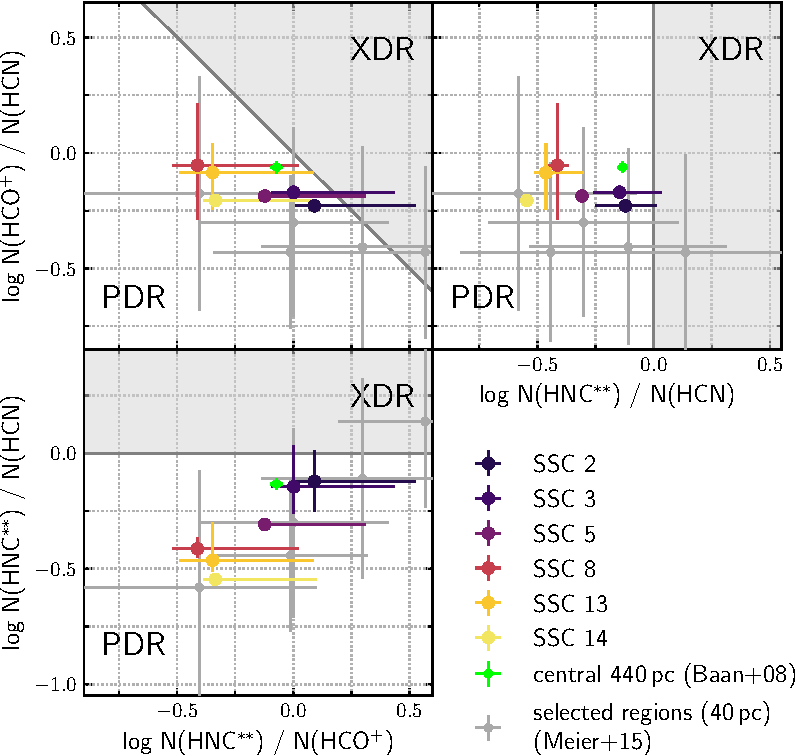
\includegraphics[width=0.8\linewidth]{thesis/images/chapters/papers/SSCs/SSCs_XDR-PDR_column_density.pdf}
    \caption[PDR--XDR chart]{PDR--XDR chart according to \citet{Loenen:2008fb} and \citet{Baan:2008hx} for ratios of HCN, HCO$^+$ and HNC column densities. In our observations, we do not observe H$^{14}$NC but H$^{15}$NC which we estimate using the isotope ratio $^{14}$N/$^{15}$N from H$^{14}$NC and H$^{15}$NC. In the plot, this is marked by $^{**}$ in the label. The correction is possible for only 6 out of 14 SSCs due to the detection rate of H$^{15}$NC. The \citet{Baan:2008hx} estimate for the central region (26\arcsec, 440\,pc) of \ngc253 extends over all SSCs and surrounding gas. The 40\,pc (2.4\arcsec) regions of \citet{2015ApJ...801...63M} focus on selected positions within \ngc253 and also cover the SSCs.
    }
    \label{SSCs: figure: XDR PDR column densities}
\end{figure*}

\citet{Loenen:2008fb} and \citet{Baan:2008hx} proposed diagnostic diagrams to infer the excitation environment in the nuclear regions of galaxies. They list different regimes for line ratios and column density ratios of HCN, HCO$^+$, HNC and CS related to PDR/XDR chemistry. These are based on PDR/XDR models by \citet{2005A&A...436..397M} and \citet{2006ApJ...650L.103M,2007A&A...461..793M} with the assumption of steady-state chemistry. 

We use these diagnostics to infer the probable excitation mechanisms in the SSCs. Figure~\ref{SSCs: figure: XDR PDR column densities} shows the relevant column density ratios of HCN, HCO$^+$ and HNC. H$^{14}$NC (4--3) at 362.63\,GHz falls outside our observed band but the we can correct the detected H$^{15}$NC using the $^{14}$N/$^{15}$N isotope ratio obtained from HCN and HC$^{15}$N.
The SSCs where all necessary lines are detected (SSCs~2, 3, 5, 8, 13, 14) all fall in the PDR regime of the model.
SSCs~2 and 3 are barely compatible with XDR conditions within $1\sigma$ errors. 
For PDRs, the HCO$^+$/HCN ratio can allow to differentiate density regimes \citep{Loenen:2008fb} where the measured $log \left( \mathrm{HCO}^+/\mathrm{HCN} \right)\sim 0$ indicates volume density $n \sim 10^5$\,\pcm3. \citet{Baan:2008hx} further utilize CS/HCN as a column density tracer with CS/HCN$\geq1$ at $N_H \GTRSIM 10^{22}$\,\pcm2 and CS/HCN$\leq1$ for lower column densities. In the SSCs~2, 3, 5, 8, 13, 14 that we can relate to PDRs, the line ratio CS/HCN$\LESS 1$ in all cases implying high column densities $\GTR 10^{22}$\,\pcm2 as is expected for this high-mass, dense environment. 
The H$_2$ column density derived from the CO intensity \citep[using $X_\mathrm{CO} = 0.5 \times 10^{20}$\,\pcm2\,(K\,\kms)][]{2013ARA&A..51..207B} is indeed between $\sim 5.1 \times 10^{22}$\,\pcm2 (SSC~5) and $\sim 2.7 \times 10^{23}$\,\pcm2 (SSC~14).

Figure~\ref{SSCs: figure: XDR PDR column densities} also shows the ratios obtained by \citet{Baan:2008hx} for the (3--2) transitions of the involved species. Their results from single dish observations cover the central 26\arcsec ($\sim 440$\,pc) and thus average all SSCs and further nuclear molecular gas. 
Reassuringly, their position for \ngc253 in the diagnostic diagrams is close to the average of our detected SSCs. The $\LESSSIM 0.2$\,dex mismatch is likely caused by the nuclear gas outside the SSCs.
Our measurements are furthermore consistent with \citet{2015ApJ...801...63M} who report the (1--0) transitions of HCN, HNC, HCO$^+$ for 10 selected regions of 2.4\arcsec ($\sim40$\,pc). Since they, too, do not observe HNC directly, we infer the HNC column density and line intensity from HN$^{13}$C and the $^{12/13}$C ratio obtained from H$^{12}$CN and H$^{13}$CN. Note that \citet{2015ApJ...801...63M} estimate their column densities assuming optically thin LTE conditions whereas we consider optical depth.

As a consistency check, we also construct Figure~\ref{SSCs: figure: XDR PDR column densities} with observational (instead of modelled) data using the line intensity ratios and find the the same qualitative result of chemistry consistent with a PDR environment. Details are discussed in Appendix~\ref{appendix: SSCs: energy source intensity}.

Finding PDR chemistry in the SSCs on parsec scales is consistent with the large scale study by \citet{2009ApJ...706.1323M} who confirm a photo-dominated chemistry for their detected typical PDR tracers the central $400-500$\,pc of \ngc253.

Obviously, the two PDR/XDR models discussed in Section~\ref{SSCs: section: CS/HCN} and here cannot simultaneously apply as they attribute different tracer properties to CS/HCN. However, it is reassuring that both models consistently favor PDR conditions in all SSCs.
For embedded (proto-)SSCs, PDR-dominated chemistry is expected although large amounts of young O/B-stars could potentially emit enough short-wavelength radiation to create a mild XDR.
As mentioned before, SSCs~$8-12$ are located close ($\LESS 0.5$\arcsec, $\LESS 8.5$\,pc) in projection to the stellar kinematic center \citep[$\alpha, \delta = 00^h47^m13.179^s, -25^\circ17^\prime17.13\arcsec$][]{MullerSanchez:2010dr} and the continuum source TH2 \citep[$\alpha,\delta = 00^h 47^m 31.2^s, -25^\circ 17^\prime 17\arcsec$;][]{1997ApJ...488..621U} proposed to be an AGN. At this location, they could be influenced by a potential AGN that may exhibit XDR properties.
\ngc253 hosts a SMBH of $\sim 8 \times 10^6$\,\Msun \citep{2006ApJ...644..914R,2014ApJ...789..124D} but shows no clear sign of even a low luminosity AGN \citep{MullerSanchez:2010dr,Gunthardt:2015ba}. 
XDR chemistry in nearby SSCs could provide hints towards a low luminosity, obscured AGN. As discussed above, both models at hand, however, exclude this possibility.

Finally, it must be noted that our finding that all SSCs (where possible) are consistent with PDR chemistry means X-rays are not the main source of energy input. It does not imply the inverse, that UV heating is the dominant energy input. Mechanical heating from e.g. shocks associated with accretion or outflows can dominate the energy budget while UV radiation only contributes.
In fact, \citet{2006ApJS..164..450M} detect typical PDR tracers in the central 200\,pc of \ngc253 but conclude that the heating is dominated by large-scale low velocity shocks as they show by comparing \ngc253 to other starbursts and the Galactic center.
This tension is solved by \citet[see their figure~10]{2015ApJ...801...63M} who could spatially separate energy sources in early ALMA observations at 3\arcsec ($\sim 50$\,pc) resolution. They draw a picture of an inner nuclear disk (where the SSCs are located) dominated by PDRs but with a contribution of wide-spread shocks. This inner nuclear disk is surrounded by an outer nuclear disk in which shocks dominate similar to bar shock regions in other galaxies.


%%%%%%%%%%%%%%%%%%%%%%%%%%%%%%%%%%%%%%%%%%%%%%%%%%%%%%%%%%%%%%%%%%%%%%%%%%%%%%%%%%%%%%%%%%%%%%%%%%%%

\subsection{Isotopic ratios and optical depth}\label{SSCs: section: optical depth}

Table~\ref{SSCs: table: ratios other} lists line ratios of the HCN isotopologues H$^{13}$CN and HC$^{15}$N with HCN. As the isotopologues are less abundant and therefore less bright, so less optically thick, such a line ratio can act as a proxy for the optical depth. 
We detect HCN/H$^{13}$CN with a large spread of $\sim$ one order of magnitude in the range $3.2-66$.
In HCN/HC$^{15}$N the ratios scatter less between $3.0-11.8$. 
Both line ratios show a similar pattern with low ratios in SSCs~13, 14, intermediate ratios in SSCs~3 and high ratios in SSC~2, 4. In SSCs~5,8, the HCN/H$^{13}$CN ratios are significantly lower than HCN/HC$^{15}$N considering the relative range of ratios observed.

Our HCN/H$^{13}$CN ratios scatter around the respective large scale ratios in the center of \ngc253 with a bias towards lower ratios. \citet{JimenezDonaire:2017eg} found HCN/H$^{13}$CN = $17 \pm 1$ and \citet{2015ApJ...801...63M} obtained HCN/H$^{13}$CN = $10-15$. Both studies cover the entire center of \ngc253 at 170\,pc (single aperture) and 35\,pc (probing 10 regions) resolution, respectively, whereas we focus on the SSCs at parsec scales.

In the simplest case where HCN is optically thick, H$^{13}$CN optically thin and the gas is perfectly mixed at a constant density, the optical depth
\begin{equation}
    \tau^{^{13}C} = T_b^{^{13}\mathrm{C}}/T_b^{^{12}\mathrm{C}}
    \label{equation: tau thin}
\end{equation}
depends on the observed intensity ratio and 
\begin{equation}
    \tau^{^{12}\mathrm{C}} = \tau^{^{13}\mathrm{C}} \times [^{12}\mathrm{C}]/[^{13}\mathrm{C}]
    \label{equation: tau thick}
\end{equation}
follow from the abundance ratio \citep[e.g.,][]{JimenezDonaire:2017eg}. Further assumptions are equal beam filling factors and a common excitation temperature for both isotopologues. The same arguments apply to HC$^{15}$N and S$^{18}$O. This simple model of optically thick main species and optically thin isotopologues is often assumed in nearby galaxies. Given the dense and compact SSCs, it provides an estimate of optical depth but may not be exactly valid.

For the abundance ratios $^{12/13}$C = [$^{12}$C]/[$^{13}$C], $^{14/15}$N = [$^{14}$N]/[$^{15}$N] and $^{16/18}$O = [$^{16}$O]/[$^{18}$O] we turn to the literature to break the degeneracy of optical depth and abundance ratio.
We adopt $^{12/13}$C = $40\pm20$ \citep[among nearby galaxies including \ngc253,][]{2014A&A...565A...3H,2010A&A...522A..62M,2019A&A...624A.125M,2019arXiv190606638T},
$^{14/15}$N = $200\pm1$\,dex \citep[and references therein, see their table~1 for an overview]{2019MNRAS.486.4805V} and
$^{16/18}$O = $130\pm40$ \citep[\ngc253;][]{2019A&A...624A.125M}.

With the arguments above we obtain $\tau_\mathrm{H^{13}CN} = 0.05 - 0.3$ and $\tau_\mathrm{HCN} = 2.0 - 12$.
SSCs 1, 3, 5, 8, 9, 11, 13 and 14 would have quite high optical depths in the $^{12}$C ($\tau_\mathrm{H^{12}CN}\GTR 5$) as well as the $^{13}$C lines ($\tau_\mathrm{H^{13}CN} \GTRSIM 0.15$) while in the other SSCs $\tau_\mathrm{H^{12}CN} \sim 1-5$ are moderately thick. SSC~10 with $\tau_\mathrm{H^{12}CN} \sim 0.6$ is marginally optically thick.
For the $^{14/15}$N ratio, $\tau_\mathrm{HC^{15}N} = 0.08 - 0.3$ or $\tau_\mathrm{HC^{14}N} = 15-66$. 
In $^{16}$O and $^{18}$O derived from SO, we obtain $\tau_\mathrm{S^{18}O} \LESS 0.1$ and $\tau_\mathrm{S^{16}O} \LESSSIM 15$.
A very low ratio in SSC~1 and corresponding high opacity ($\tau_\mathrm{S^{18}O} = 0.6$, $\tau_\mathrm{S^{16}O} = 78$) likely originates from confusion between S$^{18}$O and HC$_3$N lines.

In order to match the two estimates for $\tau_{\mathrm{HCN}}$, $^{12/13}$C on the high side and $^{14/15}$N on the low side of extra-galactic measurements would be required.
\citet{JimenezDonaire:2017eg} estimate the optical depth at $\tau_\mathrm{H^{12}CN} = 2.5$ and $\tau_\mathrm{H^{13}CN} = 0.07$ averaged over the whole center of \ngc253. The HCN opacities of SSCs~2, 4, 6 and 12 do not stand out above this large scale environment while the other SSCs show higher optical depths in HCN. As indicated above, this trend in optical depth correlates with cluster age (cf. Section~\ref{SSCs: section: other lines}).

Given the in parts high optical depths it must be noted that different species do not have to originate from the same location in the SSC cloud. If the gas density is not constant, emission from the more optically thick line originates from outer layers of the cloud. Chemical variations may thus be reflected in one line but not the other in all line ratios of this study. For instance, chemical enrichment by stellar winds of young stars within the forming cluster may affect only the inner regions of the SSC parent cloud.


%%%%%%%%%%%%%%%%%%%%%%%%%%%%%%%%%%%%%%%%%%%%%%%%%%%%%%%%%%%%%%%%%%%%%%%%%%%%%%%%%%%%%%%%%%%%%%%%%%%%

\subsection{Other lines}\label{SSCs: section: other lines}

We detect a multitude of molecular species and spectral lines in these deep observations. In the following section, we focus on a few of them.


%%%%%%%%%%%%%%%%%%%%%%%%%%%%%%%%%%%%%%%%%%%%%%%%%%%%%%%%%%%%%%%%%%%%%%%%%%%%%%%%%%%%%%%%%%%%%%%%%%%%

\subsubsection[HC3N]{HC$_3$N}\label{SSCs: section: HC3N}

HC$_3$N is a tracer for warm and dense gas \citep[e.g.][]{2018ApJS..236...40T}. It has multiple bending modes ($\nu_5$, $\nu_6$, $\nu_7$) at IR frequencies which makes it sensitive to a strong IR field and allows HC$_3$N to act as a hot dust tracer when IR cannot be observed directly due to extinction \citep{2020MNRAS.491.4573R}. UV radiation and CRs can easily destroy the molecule, so it traces shielded IR irradiated dense gas \citep[e.g.][]{2010A&A...515A..71C}. HC$_3$N abundances are enhanced in hot environments due to evaporation from dust grain mantles. Galactic detections are thus typically in hot cores \citep[e.g. Sgr~B2][]{2000A&A...361.1058D} but it was also detected in other galaxies, such as \ngc253, NGC~4418 or IC~342 \citep[e.g.][]{2011A&A...528A..30C,2011A&A...525A..89A,2005ApJ...618..259M,2007A&A...475..479A,2011AJ....142...32M}. Most often the 10--9 transition at $\sim 90$\,GHz is detected \citep[e.g.][]{2011A&A...528A..30C} but detections up to $J_{upper} \GTR 30$ are given in the literature as well as detection of the vibrational states \citep[$\nu_6$, $\nu_7$; e.g.][]{2010A&A...515A..71C,2011A&A...527A..36M,2011A&A...528A..30C}.

HC$_3$N lines are often the brightest, or at least among the brightest, lines after CO, HCN, HCO$^+$ and CS in our spectral window. This directly implies a high IR radiation field, because due to their high critical densities ($\GTR 10^8$\,\pcm3), HC$_3$N transitions cannot be purely collisionally excited; they also need to be pumped in the IR. Furthermore, we detect the (38--37) and (39--38) lines, so the temperatures must be high in order to excite these transitions (cf. Section~\ref{SSCs: section: ISM temperature}). 
The ubiquitous highly excited HC$_3$N and the observation that many SSCs contain PDRs (Section~\ref{SSCs: section: dense gas}) pose constraints on the PDR or the dense gas geometry.
High UV fluxes in a PDR can quickly dissociate HC$_3$N. Therefore, the UV field illuminating the PDRs must be either weak, or the HC$_3$N is well shielded from the photodissociating radiation, or alternatively the HC$_3$N emission is spatially separate from the PDRs.
As discussed in Section~\ref{SSCs: section: energy source}, the PDR vs. XDR discrimination only indicates the relative, not the absolute strength and does not cover mechanical heating as an energy source. In this context, the observation of bright HC$_3$N implies a weak PDR and dominant mechanical heating likely by gas accretion onto the forming SSCs and proto-stellar outflows.
On the other hand, if the HC$_3$N and the PDR traced by the HCN/HCO$^+$/HNC emission are spatially separated, the PDR can either be driven from the inside by the SSC in the center of the surrounding molecular cloud or from the outside by neighboring sources in an outer shell of the cloud. The first case implies a radially stratified model of onion-like layers with HCN/HCO$^+$/HNC in the inner irradiated region and an outer layer of HC$_3$N. In the second case, HC$_3$N is shielded inside the cloud from external radiation but HCN/HCO$^+$/HNC can be well mixed with HC$_3$N.
Without additional tracers of mechanical heating and cloud structure we currently cannot distinguish these possibilities.
At much lower resolution and for the central $400-500$\,pc, \citet{2009ApJ...706.1323M} show that the PDR tracers originate in the outer layers of UV-illuminated clouds, similar to the aforementioned onion-layer structure. Our study, however, focuses on particular sources at 200 times higher resolution which may not share this large scale structure.

The ratio of HCN over HC$_3$N might be interpreted as a ``super dense gas'' fraction or very high density to high density gas ratio. Such a ratio is, as all line ratios are, only meaningful if HCN and HC$_3$N originate from the same region. Under that assumption, HCN/HC$_3$N implies the highest fraction of very dense gas can be found in SSC~13 whereas SSC~10 would contain little very high density gas (c.f., Table \ref{SSCs: table: ratios other}).
Increasing HCN/HC$_3$N ratios should occur when a molecular cloud gets disrupted by feedback as HC$_3$N is dissociated before HCN, and even earlier the favourable conditions for IR pumping are shut down as the self-shielding of the cloud diminishes. Towards the end of a molecular cloud lifetime HCN/HC$_3$N should thus be an age tracer, and the evolutionary sequence would be $13,4,14,1,8,3,2$ from young to old. \citet{2020MNRAS.491.4573R} recently dated\footnote{Their method can only date SSCs with a significant fraction of proto-stellar contribution and thus age dating is possible only until the cluster reaches the zero age main sequence.} the super hot cores within the SSCs by the fraction of proto-stellar (inferred from the IR radiation field pumping the HC$_3$N vibrational transitions) to stellar luminosity (inferred from the ionizing luminosity), which results in an almost inverted sequence ($2,3,13,1,8,14,4$). This suggests that the HCN/HC$_3$N ratio is not a reliable age tracer, at least for the young, deeply embedded SSCs in this study. Potential causes of the mismatch are structural effects, i.e. HCN and HC$_3$N not originating from the same region, or the SSCs are to young to cause detectable effects on the HCN/HC$_3$N ratio. The latter is supported by the fact that the oldest SSCs (zero age main sequence SSCs $6,7,9,10,11,12$, according to \citealt{2020MNRAS.491.4573R}) are consistently found at higher HCN/HC$_3$N than the younger proto-SSCs ($1,2,3,4,8,13,14$) by factors of $\sim1-4$.

HCN/HC$_3$N ratios of $3-4$ are commonly reported in nearby galaxies on scales of hundreds of pc for low-J and high-J HC$_3$N lines \citep[NGC~4418, IC~342;][]{2005ApJ...618..259M,2007A&A...475..479A,2010ApJ...725L.228S,2011AJ....142...32M}. Apart from SSC~13, the other SSCs show considerably larger ratios than this nearby galaxy average.
In the center of \ngc253, HCN/HC$_3$N$\sim10$ has been measured by \citet{Lindberg:2011kk} over 25\arcsec (425\,pc). Hence, HC$_3$N/HCN in the SSCs does deviate in both directions by factors of a few from the large scale average.

The detection of vibrationally excited HC$_3$N is among the first extragalactic of such detections \citep{2010A&A...515A..71C,2011A&A...527A..36M,2011A&A...528A..30C}. It is especially noteworthy that we detect high-J vibrationally excited lines which requires high temperatures and a strong IR field. With these observations, we can confirm that HC$_3$N is associated with dense starforming gas and a starbursting environment.


%%%%%%%%%%%%%%%%%%%%%%%%%%%%%%%%%%%%%%%%%%%%%%%%%%%%%%%%%%%%%%%%%%%%%%%%%%%%%%%%%%%%%%%%%%%%%%%%%%%%

\subsubsection{Sulfur chemistry}\label{SSCs: section: sulfur chemistry}

Chemical studies suggest that the fractional abundance of CS is sensitive to both the abundances of sulfur and oxygen \citep{1982ApJS...48..321G}. SO$_2$ is related to turbulent gas near stellar activity \citep{Minh:2016dx}. In undisturbed gas, sulfur is thought to be depleted onto ice grain mantles and sulfur-bearing species may act as chemical clocks in the evolution of SF. SO and SO$_2$ form from grain-evaporated H$_2$S and abundances increase with time until at later times most of the sulfur is captured in CS, H$_2$CS and OCS \citep{1998A&A...338..713H}. The SO/SO$_2$ ratio may act as a crude clock with lower ratios towards later times \citep{1997ApJ...481..396C}. SO$_2$ is also used as a tracer for low velocity outflows in stellar cores \citep{Wright:1996hi,Liu:2012ex}.

SO/SO$_2$ and CS/SO$_2$ line ratios are given in Table~\ref{SSCs: table: ratios other} for the ground state of SO, \cs and SO$_2 11_{4,8}-11_{3,9}$.
The SO/SO$_2$ ratios varies by a factor of $\sim5$ across SSCs and $\sim 7$ in CS/SO$_2$. Both ratios follow the same trend with low ratios in SSCs~1, 3 and 4, and highest ratios in SSCs~5, 8 and 11. If SO/SO$_2$ relates to age, the former are older while the latter are younger. This is in contrast to the HC$_3$N age dating and \citet{2020MNRAS.491.4573R} which suggest exactly the opposite relation.

\citet{2005ApJ...620..210M} studied the sulfur chemistry in \ngc253 at $200-500$\,pc resolution which provides an average value for all SSCs and surrounding gas. They find fractional abundances CS/SO$_2 = 5$ and SO$_2$/SO = 1 which is considerably lower than our average line ratios over the detected SSCs of CS/SO$_2 = 9.2$ and SO$_2$/SO = 3.1. It must be noted that \citet{2005ApJ...620..210M} observed less excited gas with transitions up to CS(5--4), SO($4_3-3_2$), SO$_2$($8_{2,6}-8_{1,7}$) whereas we cover transitions above those and up to CS(7--6), SO($8_8-7_7$) and SO$_2$($17_{4,14}-17_{3,15}$). Therefore, excitation effects may shift the line ratios. Given the uncertainties, the enhanced ratios in the SSCs could be explained by a factor of two depletion of SO$_2$ or factors of $2-3$ enhancement of SO and CS relative to the large scale average from \citet{2005ApJ...620..210M}.


%%%%%%%%%%%%%%%%%%%%%%%%%%%%%%%%%%%%%%%%%%%%%%%%%%%%%%%%%%%%%%%%%%%%%%%%%%%%%%%%%%%%%%%%%%%%%%%%%%%%

\subsubsection{Vibrationally excited species}\label{SSCs: section: vibrational excitation}

The vibrationally excited lines of HCN and HC$_3$N have high critical densities (e.g. HCN $\nu_2=1, l=1f$ $n_\mathrm{crit}\GTR 10^{10}$\,\pcm3) which makes purely collisional excitation unlikely. Instead radiative excitation, particularly in the IR, is required (e.g. at 14\,\mum for HCN $\nu_2=1, l=1f$, \citealt{1986ApJ...300L..19Z}). These vibrational lines have been frequently observed towards nuclei of nearby (U)LIRGs \citep{2010ApJ...725L.228S,2013ApJ...764...42S,2015A&A...584A..42A,2016ApJ...825...44I,2017ApJ...849...29I,2018A&A...609A..75F} but also in Galactic hot cores \citep{2011A&A...529A..76R,2011A&A...527A..68R,2011A&A...536A..33R,2015A&A...584A..42A}. In buried galactic nuclei powered by AGNs or starbursts, the dust emission can become optically thick and very effectively pump vibrationally excited HCN and HC$_3$N lines similar to a greenhouse \citep[e.g.][]{2019ApJ...882..153G}. However, no AGN, not even a low luminosity AGN, has been found in \ngc253 yet \citep{MullerSanchez:2010dr,Gunthardt:2015ba}.

\begin{table}[ph]
    \centering
    \begin{threeparttable}
        \caption[Ro-vibrational over vibrational excitation fractions]{Integrated intensity ro-vibrational over rotational excitation fraction for selected HCN and HC$_3$N lines. The ro-vibrational line used for the respective ratio is given in the second row.
        \label{SSCs: table: ratios vibrational excitation}}
        
        \begin{tabular}{r|cccc}
            \toprule
            SSC & HCN/HCN*  & HCN/HCN* & HC$_3$N/HC$_3$N* & HC$_3$N/HC$_3$N* \\
             & $\nu_2=1$, $l=1f$ & $\nu_2=2$, $l=2f$ & $\nu_7=1$, $l=1f$ & $\nu_7=2$, $l=2f$ \\
            \midrule
1 & $3.7^{+0.5}_{-0.3}$ & $30.1^{+15.4}_{-9.9}$ & ... & ...\\
2 & $5.7^{+0.3}_{-0.4}$ & $28.6^{+3.9}_{-3.4}$ & $1.6^{+0.2}_{-0.3}$ & $2.1^{+0.3}_{-0.4}$\\
3 & $3.1^{+0.3}_{-0.2}$ & $24.2^{+8.6}_{-4.8}$ & $1.1^{+0.2}_{-0.1}$ & $3.1^{+0.9}_{-0.6}$\\
4 & $2.9^{+0.7}_{-1.2}$ & $8.4^{+2.4}_{-3.3}$ & $2.9^{+0.8}_{-0.5}$ & $3.1^{+0.8}_{-0.5}$\\
5 & $7.9^{+0.1}_{-0.2}$ & $81.4^{+13.6}_{-10.5}$ & $2.2^{+0.1}_{-0.2}$ & $5.1^{+1.0}_{-0.7}$\\
6 & ... & ... & ... & ...\\
7 & ... & ... & ... & ...\\
8 & $2.7^{+1.8}_{-1.8}$ & $58.7^{+50.6}_{-38.4}$ & $2.2^{+1.0}_{-0.3}$ & ...\\
9 & ... & ... & ... & ...\\
10 & ... & ... & ... & ...\\
11 & $16.2^{+9.3}_{-7.5}$ & ... & $6.1^{+1.4}_{-0.7}$ & ...\\
12 & ... & ... & ... & ...\\
13 & $1.4^{+0.2}_{-0.2}$ & $9.7^{+1.6}_{-1.5}$ & $1.4^{+0.1}_{-0.1}$ & $2.2^{+0.2}_{-0.2}$\\
14 & $2.0^{+0.1}_{-0.0}$ & $17.0^{+2.4}_{-2.9}$ & $1.9^{+0.1}_{-0.1}$ & $4.8^{+0.2}_{-0.2}$\\
            \bottomrule
        \end{tabular}
    \end{threeparttable}
\end{table}



For HCN and HC$_3$N, we detect vibrationally excited lines in 6 out of 14 SSCs for HCN$^*$ ($\nu_2=1$, $\nu_2=2$) and 8/14 ($\nu_6=1$), 8/14 ($\nu_7=1$), 6/14 ($\nu_7=2$) in HC$_3$N$^*$ (cf. Table~\ref{SSCs: table: intensities}), so we can estimate the fraction of ro-vibrational vs. purely rotational excitation.
The ro-vibrational lines are very crowded, however, and blend into compact blocks of emission in some SSCs. All vibrational bending modes ($f$ and $e$) for each $\nu$ level are detected with one line only which makes it difficult to disentangle the spectra. The theoretical relationship between vibrational modes within the same ro-vibrational species as implemented in \xclass constrains the relative line strengths but systematic effects might remain.
Table~\ref{SSCs: table: ratios vibrational excitation} lists the rotational over ro-vibrational line ratios of the $f$ bending modes.
In \hcn $\nu_2=1$, $l=1f$ we find line ratios of HCN/HCN$^*$ typically in the range $\sim 1.5-8$ where detected. This corresponds to vibrationally excited rotational state fractions of $\sim 10-40$\%. The higher value of $\sim 16$ in SSC~11 indicates close to negligible relative importance of vibrational excitation of only 5\%. The higher \hcn $\nu_2=2$, $l=1f$ state is negligible relative to HCN and \hcn $\nu_2=1$, $l=1f$ according to the high intensity ratios of $\GTR 8$.

For HC$_3$N vibrational excitation is a more important mechanism relative to purely rotational excitation: where detected, the line ratios between purely rotational and vibrationally excited variant are low at typically $\sim 1 - 3$ corresponding to fractional contributions of the vibrationally excited lines of $25\%-50\%$.
These high fractions of emission in vibrationally excited lines hints at strong IR (around $\sim 14$\,\mum) fields in the SSCs. Such an IR environment can be expected for forming SSCs as they are still deeply embedded \Leroy{p} and undetected in optical and near-IR \citep{2017ApJ...835..265W}. Emission by the forming stars is trapped inside the SSC by high opacity without leaking outside yet. \Leroy{t} argue for high optical depths in the IR due to their detection of 350\,GHz emission at $\tau \sim 0.1$ which implies $\tau = 5-10$ at the peak of the dust SED ($20-30$\,\mum). Such opacities are more than enough to create the aforementioned conditions for 14\,\mum trapping and IR pumping.

\citet{2020MNRAS.491.4573R} recently investigated the super hot cores in the SSCs using HC$_3$N. Their spectral window partially overlaps with our setup but we detect further vibrationally excited HC$_3$N lines as listed in Table~\ref{SSCs: table: intensities}.
From our detections, we can confirm their observation that SSCs~6 and 7 lack HC$_3$N even in the ground state and SSCs~9,10 and 12 do not show vibrationally excited HC$_3$N. However, we detect two HC$_3$N$^*$ species in SSC~11. Qualitatively, our HC$_3$N detection rates confirm the conclusion of \citet{2020MNRAS.491.4573R} that SSCs~6, 7, 9, 10, 11 and 12 are older than SSCs~1, 2, 3, 4, 5, 8, 13 and 14.


%%%%%%%%%%%%%%%%%%%%%%%%%%%%%%%%%%%%%%%%%%%%%%%%%%%%%%%%%%%%%%%%%%%%%%%%%%%%%%%%%%%%%%%%%%%%%%%%%%%%

\subsection{ISM temperature}\label{SSCs: section: ISM temperature}

\begin{table}[ph]
    \centering
    \begin{threeparttable}
        \caption[Fitted excitation temperatures]{Excitation temperatures obtained by \xclass fitting.
        \label{SSCs: table: temperatures}}
        
        \begin{tabular}{r|cccc}
            \toprule
            SSC & H$_2$CS & SO$_2$ \\
            \midrule
 1 &                 ... &  84$^{+ 25}_{- 14}$\\
 2 & 103$^{+ 60}_{- 23}$ & 114$^{+ 11}_{- 14}$\\
 3 &              $\GTR 242$ &  91$^{+ 13}_{-  7}$\\
 4 &              $\GTR 160$ & 191$^{+ 35}_{- 32}$\\
 5 &              $\GTR 237$ & 134$^{+ 20}_{- 26}$\\
 6 &                 ... &                 ...\\
 7 &                 ... &                 ...\\
 8 & 248$^{+166}_{- 75}$ & 129$^{+ 11}_{- 23}$\\
 9 &                 ... &                 ...\\
10 &                 ... &  47$^{+ 72}_{- 11}$\\
11 &                 ... &                 ...\\
12 &                 ... &                 ...\\
13 &              $\GTR 226$ & 122$^{+ 25}_{- 21}$\\
14 & 141$^{+ 15}_{- 16}$ & 228$^{+ 15}_{- 20}$\\
            \bottomrule
        \end{tabular}
    \end{threeparttable}
\end{table}


\begin{figure*}
    \centering
    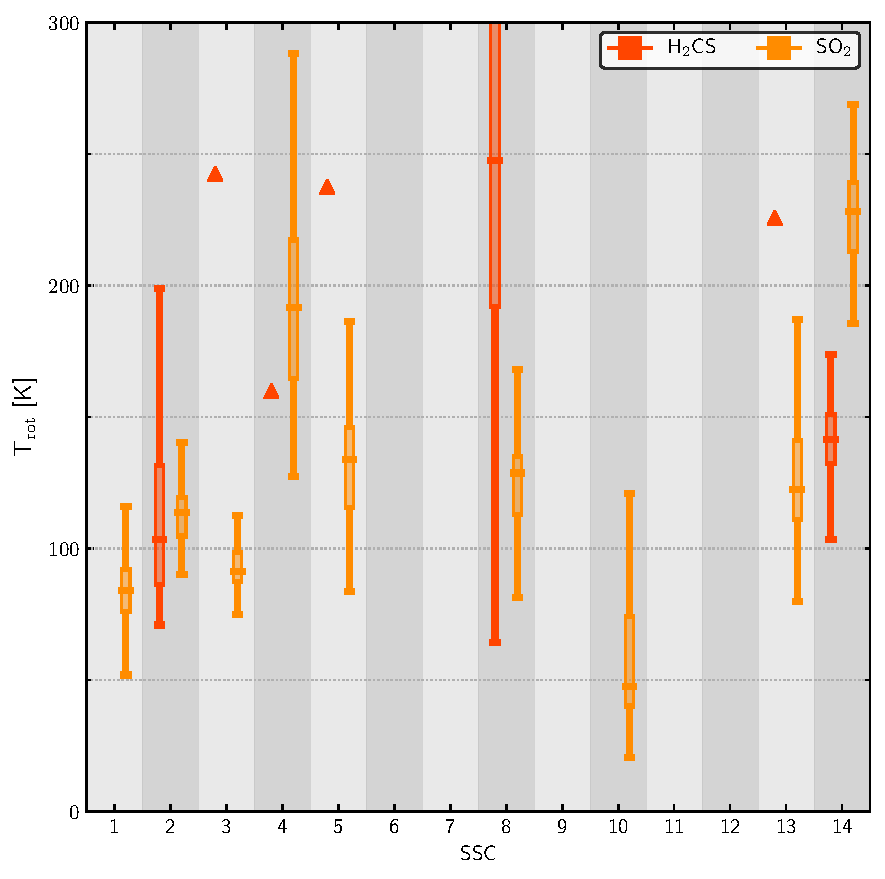
\includegraphics[width=0.75\linewidth]{thesis/images/chapters/papers/SSCs/SSCs_compare_temperatures.pdf}
    \caption[SO$_2$ and H$_2$CS rotational temperature comparison]{Comparison of the rotational temperatures derived from SO$_2$ and H$_2$CS. Boxplots show the distribution of the 100 fit iterations: a vertical line extends over the full range of values, the second and third quartile are represented by a box with the median as a horizontal line. Triangles represent lower limits (16$^{th}$ percentile) in the cases where the temperature is weakly constrained.}
    \label{SSCs: figure: temperatures}
\end{figure*}

The temperatures derived by \xclass for H$_2$CS and SO$_2$ are given in Table~\ref{SSCs: table: temperatures} and also plotted in Figure~\ref{SSCs: figure: temperatures} for comparison.

The detected SO$_2$ lines span a range in $\mathrm{E_{lower}}$ of $\sim40$\,K to $\GTR 300$\,K and should therefore allow for a good estimate of the SSCs temperatures. In practise, SO$_2$ is detected in only 11 out of 14 SSCs but confines the temperature to typically $\pm 20$\,K ($16^\mathrm{th}$ to $84^\mathrm{th}$ percentile) if detected.
In SSCs~11 and 12, the SO$_2$ lines are detected but do not allow for a robust temperature estimation as the S/N is too low.
In the LSB, the detected thioformaldehyde (H$_2$CS) lines span $\mathrm{E_{lower}} = 50-770$\,K which also provides enough range for good temperatures estimations. In SSCs~3, 4, 5 and 13, $\mathrm{T_{rot}}$ is weakly constrained and we report lower limits of the obtained XCLASS results. In SSCs~1, 6, 7, 9, 10, 11 and 12 H$_2$CS is not detected.

The rotational temperatures inferred from SO$_2$ and H$_2$CS (where possible as discussed above) do only partially agree (SSCs~2, 4, 8). In SSCs~3, 5 and 13, the lower limits on H$_2$CS temperature are substantially higher than the inferred SO$_2$ temperature. In SSC~14, $\mathrm{T_{rot}}$ is $\sim 85$\,K higher in SO$_2$ than in H$_2$CS. It must be stressed here that further radiative transfer modelling is required to translate $\mathrm{T_{rot}}$ to kinetic gas temperature $\mathrm{T_{kin}}$ and allow for fair comparison across species. Rotational temperatures provide a lower limit to the kinetic gas temperature. 
For a physical interpretation, it needs to be considered that SO$_2$ is fitted with optical depths of $3- \GTR 5$ in all SSCs. All reported temperatures thus correspond to outer gas layers of an SSC rather than its core temperature which might be different due to internal heating (e.g. feedback).

The mean rotational temperature over the SSCs with good estimates is 127\,K in SO$_2$. The common excitation temperature of 130\,K assumed for all other rotational species is therefore a good common estimate.
The molecular gas in SSC~14 is most likely significantly hotter than in the other SSCs. This is in line with the rich chemistry (high species detection rate) and in most regards more extreme nature of this source. Similarly, SSC~10, the coolest SSC in the sample is among the faintest SSCs in most lines and has low line detection rates. SSC~4 shows surprisingly high temperatures given that it is average in all other quantities in this study and \Leroy{t}. The other SSCs are similar in temperature at $\sim 90$\,K (SSC~1, 3) or $\sim 115-130$\,K (SSC~2, 5, 8, 13).

In the Central Molecular Zone (CMZ) of the Milky Way, an environment similar to the center of \ngc253, \citet{2018ApJS..236...40T} found a strong positive correlation of HC$_3$N (10--9) with temperature. If this correlation extends to high-J lines of HC$_3$N, it would imply a high temperature in SSC~14, somewhat elevated temperatures in SSC~5 and 13, but lower temperatures in SSCs 1, 2, 3, 4, 8, 9, 10, 11 and 12. For SSC~6 and 7, neither of the two HC$_3$N lines are detected.
Such an HC$_3$N -- temperature correlation is not present in our data. SSC~14 is indeed hot and bright in HC$_3$N, but there are no elevated temperatures in SSC~5 and 13. The high temperature in SSC~4 is matched by HC$_3$N line brightness and column density marginally different from SSC~2 or 3 with much lower temperatures.
Hence, a potential HC$_3$N -- temperature correlation does not extend to the high-J lines ($\mathrm{J_u}=38$ with $\mathrm{T_{ex}}=307$\,K and $\mathrm{J_u}=39$ with $\mathrm{T_{ex}}=323$\,K) that we observed here.

Our results of an average $\mathrm{T_{rot}}\sim 130$\,K is consistent with \citet{2020MNRAS.491.4573R}, the only other temperature measurement on cluster scales, who find HC$_3$N rotational temperatures of $107\pm22$\,K to $125\pm45$\,K and dust temperatures of $200-375$\,K. Considering that $\mathrm{T_{rot}}$ is a lower limit to $\mathrm{T_{kin}}$, the molecular gas is at similar temperatures to the dust and probably thermally coupled.


%%%%%%%%%%%%%%%%%%%%%%%%%%%%%%%%%%%%%%%%%%%%%%%%%%%%%%%%%%%%%%%%%%%%%%%%%%%%%%%%%%%%%%%%%%%%%%%%%%%%

\section{Summary}\label{SSCs: section: summary}

We present high-resolution ALMA observations of the SSCs in the starbursting center of \ngc253. Our spectral setup in band~7 covers a wealth of molecular species and pushes at resolving the compact (proto-) super star clusters with 2.5\,pc spatial resolution. In spectra focused on the SSCs, we detect up to 55 lines of 14 species. Fits to the spectra using modelling in \xclass allow us to independently study observation-based line ratios and modelled physical quantities.

The SSCs differ significantly in chemical complexity between 5 and 15 detected species. In CO, HCN, HCO$^+$ and CS, we detect multiple components and potential signs of self-absorption in HCN and HCO$^+$ in four SSCs. The other species are associated in velocity with the same CO/HCN/HCO$^+$/CS component or the absorption component of present.

The line ratios CO/HCN, CO/HCO$^+$ of $\sim 1-10$ are low implying high dense gas fractions. HCN/HCO$^+$ is consistent with unity in all but one clusters and most likely caused by high opacity. CS/HCN scatters significantly across SSCs and does not correlate with other properties aside from the number number of detected species. Its tracer properties remain unclear.

All SSCs favor PDR chemistry over XDR chemistry as indicated by combinations of the line ratios of HCN, HCO$^+$, HNC and CS in comparison to models \citep{Loenen:2008fb,Baan:2008hx}. According to these models, our data favors densities of $\sim 10^5$\,\pcm3. The SSCs close to the central SMBH at projected distances $\LESS 8.5$\,pc are inconsistent with XDR chemistry induced by a potential low luminosity AGN. \ngc253's putative AGN continues to be elusive.

Opacities derived from HCN and HC$^{13}$N fall in the high optical depth regime with $\tau \GTRSIM 1$ to $\tau \GTR 10 $ in HCN and up to $\tau = 0.3$ in H$^{13}$CN and HC$^{15}$N.

We detect bright HC$_3$N in highly excited states in many SSCs which implies high IR radiation fields and gas temperatures. This is at odds with finding PDR chemistry as the UV flux in PDRs can dissociate HC$_3$N. Potential solutions to this discrepancy are that mechanical heating dominates the energy input over a weak UV field or detected HC$_3$N and HCN/HCO$^+$/HNC/CS emission originates from different locations in the cloud governed by opacity.

Vibrationally excited lines of HCN and HC$_3$N are frequently detected (in 6-8 of 14 SSCs) in our observations. The fraction of vibrational excitation of a rotational state can be significant in some SSCs at order $10-30$\%. The excitation of these lines is likely caused by strong IR radiation fields that are trapped by a greenhouse effect due to high continuum opacities.

The gas in the SSCs is hot as indicated by SO$_2$ rotational temperatures of $\sim 130$\,K on average.

The presented observations demonstrate the power of ALMA to zoom into some of the most actively starforming regions in the local universe.


%%%%%%%%%%%%%%%%%%%%%%%%%%%%%%%%%%%%%%%%%%%%%%%%%%%%%%%%%%%%%%%%%%%%%%%%%%%%%%%%%%%%%%%%%%%%%%%%%%%%

%************************************************

\chapter{The turbulent gas structure in the centers of \ngc253 and the Milky Way}
\chaptermark{turbulent gas structure in galaxy centers}
\label{chapter: dendro}

%************************************************

\begin{papernote}
This chapter including appendix~\ref{appendix: dendro} comprises the article of the same title submitted the to Astrophysical Journal. The submitted paper has been reformatted to match the style of this thesis.
\end{papernote}


\begin{paperabstract}
We compare the molecular cloud properties in the starbursting center of \ngc253 and the Milky Way Galactic Center (GC) on scales of $\sim1$\,pc to several hundred pc by using resolution-, area- and noise-matched datasets.
Using dendrograms, we retrieve the hierarchical structure of the molecular interstellar medium in these galaxies from matched observations in \co10 and \co32.
We find that the size (R) -- line width ($\sigma$) relations in \ngc253 and the GC are similar in slope but \ngc253 has a significant offset towards larger line widths by factors of $\sim2-3.5$. The size--line width relation in \co32 is steep ($\sigma \propto R^{0.65\pm0.01}$ in \ngc253, $\sigma \propto R^{0.71\pm0.03}$ in the GC) but consistent with previous estimates in other molecular tracers. In \co10, the relations are steeper at $\sigma \propto R^{0.82\pm0.02}$ in \ngc253 and $\sigma \propto R^{0.84\pm0.09}$ in the GC.
The other structural properties of \ngc253 and the GC are very similar, including the size--luminosity relations as well as column density, volume density and mass probability density functions.
The size--line width coefficient ($\sigma^2/R$) dependency on column density $N$ shows that the increased line widths in \ngc253 originate in low column density gas ($N \LESSSIM 3 \times 10^{22}$\,\sqcm). 
In \ngc253, this analysis further implies a high external pressure ($P_\mathrm{ext} \sim 10^{7-7.5}$\,K\,\pcm3) and a significant amount of unbound (non-self-gravitating) molecular gas that is characterized by high velocity dispersion.
The unbound gas most likely corresponds to the known molecular outflows and potential diffuse molecular gas.
The excess kinetic energy of the unbound molecular gas in \ngc253 relative to the GC is most plausibly supplied by the starburst in the former as we show through estimation of the involved kinetic energies.
\end{paperabstract}


%%%%%%%%%%%%%%%%%%%%%%%%%%%%%%%%%%%%%%%%%%%%%%%%%%%%%%%%%%%%%%%%%%%%%%%%%%%%%%%%%%%%%%%%%%%%%%%%%%%%

\section{Introduction} \label{dendro: section: introduction}

The centers of spiral galaxies are special places in the galactic environment as their physical properties differ in many ways from the disk and halo. Even visible by the naked eye in nearby galaxies, stellar surface brightness is significantly higher in galaxy centers than in the disk. 
In strongly barred galaxies, the bar helps drive gas to the galaxy center \citep[e.g.][]{2019A&A...623A..79C}. This results in the formation of ring-like structures that are often connected to the outer galaxy by dust lanes and gas streams \citep[e.g.][]{2001AJ....121..225B,2017MNRAS.471.4027B,2017MNRAS.470.3819B,2005A&A...429..141K,2013A&A...555L...4C,2011A&A...529A..45V}. 
As all massive galaxies are thought to host a supermassive black hole (SMBH) in their centers \citep{2013ARA&A..51..511K}, the picture is even more complex, especially if the SMBH is actively accreting, i.e. it is visible as an active galactic nucleus (AGN) and affecting its surroundings through AGN feedback. 
In addition, close to the bottom of the galactic gravitational potential (on $10^2$\,pc scales), the rotation curve transitions from its typically flat shape to solid body\linebreak[4] rotation -- this changes the dynamical forces acting on the gas \citep[e.g.][]{2017MNRAS.466.1213K}. All these properties (and more) create a unique gravitational, dynamical and highly complex environment for the star formation life cycle.

As a result of these conditions, the gas contents of galactic centers are typically characterised by more extreme properties than the surrounding disk: higher densities, higher temperatures, and higher velocity dispersion and turbulence \citep[e.g.][]{Morris:1996db,2000ApJ...536..357M,2001ApJ...562..348O,2012MNRAS.425..720S,2013PASJ...65..118S,2016A&A...586A..50G,2017ApJ...850...77K,2019MNRAS.483.4291C,2019ApJ...871..170M}. According to star formation prescriptions that focus on density \citep{2013MNRAS.429..987L,Kennicutt:1998id,2005ApJ...630..250K,Krumholz:2012ja,Lada:2012it,2010ApJ...724..687L} an elevated star formation rate (SFR) would consequently be expected which is not always found.

Galactic centers and (nuclear) starbursts are often referred to as analogs for high-z star forming galaxies at the peak of the cosmic star formations history \citep[e.g.][]{2013MNRAS.435.2598K}. Upon closer inspection, however, these proposed high-z analogs can differ significantly in properties of the ISM, stellar content, star formation process and feedback \citep[e.g.][]{2017MNRAS.471.2311L,2019ApJ...872..146J}.

Studies of star forming regions within the Milky Way allow for very high spatial resolution and show that it is necessary to resolve individual clouds at pc-scales to correctly capture the physical processes that are relevant for the star formation process. 
With the newest and upcoming generations of radio telescopes it is now feasible to resolve the necessary scales in nearby galaxies such as \ngc253.

For the first time, we conduct a matched comparison of the properties of the turbulent molecular ISM at parsec scale resolution in the nearby universe and interpret the results in the context of the star formation process.
In this work, we focus on the Milky Way's more quiescent Galactic Center (GC) and the center of \ngc253 which harbors a nuclear starburst.

This paper is structured as follows: In Section~\ref{dendro: section: data}, we describe the datasets of \ngc253 and the GC. The methodological approach of the dendrogram technique and how to construct size--line width relations is laid out in Section~\ref{dendro: section: structural analysis}. We show the results (Section~\ref{dendro: section: results}), discuss them in Section~\ref{dendro: section: discussion} and summarise our work in Section~\ref{dendro: section: summary}. The appendix~\ref{appendix: dendro: structure definition} lists technical details and presents checks of the used methods.

\subsection{The Galactic Center}

At a distance of only $\sim8.2$\,kpc, the GC is the nearest galactic center and can be observed at unrivaled resolution.
The GC (central $\sim 1$\,kpc) hosts a significant fraction of order 10\% of the entire molecular gas mass of the Milky Way with $\sim 6-8 \times 10^7$\,\Msun of molecular gas in the Central Molecular Zone \citep{1998ApJS..118..455O,Morris:1996db,2007A&A...467..611F}.
Compared to the high mass of dense molecular gas available for star formation, it shows a low SFR ($\sim 0.1$\Msunyr) and SFR density despite hosting many of the galaxy's most massive and dense molecular clouds \citep[e.g.][]{2013MNRAS.429..987L,2017MNRAS.469.2263B}.
As a result, the star formation efficiency of the dense gas is also very low compared to the Galactic disk \citep[e.g.][]{2013MNRAS.429..987L}.
This discrepancy has been attributed to cloud stabilization by turbulent pressure and a quiescent phase of episodic \citep[e.g.][]{2015MNRAS.453..739K,2017MNRAS.466.1213K} or stochastic \citep[e.g.][]{2019MNRAS.484.1213S} gas processes and star formation.
Increasing evidences for winds and outflows from the GC hint towards more active star formation (or AGN activity) in the past \citep[e.g.][]{2019arXiv191106864L,2019MNRAS.482.4813S}.

Throughout this paper, we adopt the recent precise distance measurement of 8.178\,kpc for the GC \citep{2019A&A...625L..10G} for which 10\,pc correspond to 4.2\arcmin.
We refer to Sgr~A* at $l, b = 359.94422947^\circ, -0.04615714^\circ$ as the ``central position'' of the GC \citep{2011AJ....142...35P}. For the systemic velocity we use 0\,\kms.


\subsection{\ngc253 and its starbursting center}

\ngc253 is one of the nearest starburst systems (SFR $\sim 2$\,\Msunyr in the central $\sim 500$\,pc) at a distance of 3.5\,Mpc \citep{Rekola:2005ha} and hosts a collection of dense, massive molecular clumps associated with star formation \citep[e.g.][]{Sakamoto:2011et,2017ApJ...849...81A}. \citet{2018ApJ...869..126L} showed that these clumps contain 14 forming super star clusters (SSCs). With these properties, \ngc253 is considered one of the prototypical bar-fed nuclear starburst galaxies.
A star formation driven galactic wind emerges from the central $\sim 200$\,pc of \ngc253 that has been characterized in H$\alpha$, X-ray, as well as neutral and molecular gas emission \citep[e.g.][]{Sharp:2010jl,Turner:1985iy,Sturm:2011jb,Strickland:2000wd,Strickland:2002kp, Westmoquette:2011bp,2000ApJS..129..493H,2013Natur.499..450B,2017ApJ...835..265W,2019ApJ...881...43K,2006ApJ...636..685S}. 
Studies of the molecular gas phase in \ngc253 demonstrated that its central starburst occurs within a molecular gas reservoir of $\sim 3-4 \times 10^8$\,\Msun \citep{1996A&A...305..421M,Leroy:2015ds,2018ApJ...860...23P,2019ApJ...881...43K} and refueled by gas accretion along the bar \citep{2004ApJ...611..835P}.
The inclination of $i = 78^\circ$ makes \ngc253 an ideal target to compare to the Milky Way GC at $i \sim 90^\circ$ because the geometric corrections are relatively small ($\sin [78^\circ] = 0.98 \sim \sin [90^\circ]$).

For the remainder of this paper, we refer to the central $\sim 800$\,pc of \ngc253 where the starburst is located simply as \ngc253.
The ``central position'' of \ngc253 denotes the kinematic center at $\alpha, \delta = 00^h47^m33.134^s, -25^\circ17^m19.68^s$ as identified in \citet{MullerSanchez:2010dr} at a systemic velocity of 250\,\kms.
At a distance of 3.5\,Mpc \citep{Rekola:2005ha}, 10\,pc correspond to 0.59\arcsec.


%%%%%%%%%%%%%%%%%%%%%%%%%%%%%%%%%%%%%%%%%%%%%%%%%%%%%%%%%%%%%%%%%%%%%%%%%%%%%%%%%%%%%%%%%%%%%%%%%%%%
% DATA
%%%%%%%%%%%%%%%%%%%%%%%%%%%%%%%%%%%%%%%%%%%%%%%%%%%%%%%%%%%%%%%%%%%%%%%%%%%%%%%%%%%%%%%%%%%%%%%%%%%%

\section{Data}
\label{dendro: section: data}

\begin{table}
    \centering
    \footnotesize
    \begin{threeparttable}
        \caption[Details of the datasets used in the dendrogram analysis]{Details of the datasets used in this analysis.
        \label{dendro: table: 1}}
        
        \begin{tabular}{llccccll}
            \toprule
            set & source & line & \multicolumn{2}{c}{resolution} & noise$^b$ & reference & ALMA ID\\
	        &&& spectral & physical$^a$ &      &&\\
	        &&& [\kms]   & [pc]         & [mK] &\\
            \midrule
{\parbox[t]{2mm}{\multirow{2}{*}{\rotatebox[origin=c]{90}{low}}}} & GC & \co10 & 5.0 & 32.0 & 38 & \textsc{COGAL} \citet{2001ApJ...547..792D} &\\
& \ngc253 & \co10 & 5.0 & 32.0 & 38 & \citet{2013Natur.499..450B} & 2011.1.00172.S\\
\rule{0pt}{4ex} 
{\parbox[t]{2mm}{\multirow{2}{*}{\rotatebox[origin=c]{90}{high}}}} & GC     & \co32 & 2.5 & \phantom{3}3.0 & 115 &  Eden et al., (in prep) &\\
& \ngc253 & \co32 & 2.5 & \phantom{3}3.0 & 115 & \citet{2019ApJ...881...43K} & 2015.1.00274.S\\
            \bottomrule
        \end{tabular}
	    \begin{tablenotes}
	        \item[a] FHWM of the circular beam.
            \item[b] Root mean square noise in line-free channels after matching the noise by adding beam-correlated Gaussian noise to the GC data.
        \end{tablenotes}
    \end{threeparttable}
\end{table}

Our goal is to measure if and how the size--line width relation differs between \ngc253 and the Galactic Center. For a robust comparison, we need to match the data by comparing the same tracers at the same resolution. CO line emission is the standard tracer molecule for the diffuse to moderately dense molecular medium. We use \co10 for a low resolution comparison and \co32 for a high resolution comparison.

For \ngc253, we use the ALMA \co10 observations from \citet{2013Natur.499..450B}, \citet{Leroy:2015ds} and \citet{2015ApJ...801...63M} and the ALMA \co32 from \citet{2019ApJ...881...43K}. We refer to those papers for details of the data reduction and imaging. 

The \textsc{COGAL} survey imaged the entire Galactic plane in \co10 including the GC using the 1.2\,m Millimeter-Wave Telescope at the CfA \citep{2001ApJ...547..792D}. The \textsc{CHIMPS2} project (Eden et al., in prep.) extends the \textsc{CHIMPS} \co32 Galactic plane survey \citep{2016MNRAS.456.2885R} at the James Clerk Maxwell Telescope into the inner Galactic plane and the Central Molecular Zone building upon the data reduction recipe of COHRS \citep[CO high-resolution survey of the Galactic plane;][]{2013ApJS..209....8D}.
It must be noted that the \co10 COGAL survey undersamples the Galactic plane at $\sim 1$ beam spacing which was then interpolated to obtain a filled map whereas the other datasets (CHIMPS2, \ngc253 ALMA) are fully sampled.

Since we aim to carefully compare two environments in two galaxy centers, we match the data as closely as possible to eliminate potential artifacts. Specifically, we match spatial and spectral resolution, pixel scale, orientation with respect to the galactic plane, field of view (FoV) and noise.

\begin{enumerate}[noitemsep,topsep=0pt]
\item[(1)] The images are smoothed to circular beams with the highest possible common resolution (32\,pc for \co10 and 3.0\,pc for \co32).
\item[(2)] The images are then reprojected onto a common pixel grid aligned with galactic longitude and latitude. Pixel scales are 6.4\,pc and 0.6\,pc for \co10 and \co32, respectively (factor 5 oversampling).
\item[(3)] The spectral resolution is matched to 5.0\,\kms for \co10 and 2.5\,\kms for \co32 and reprojected on the same grid with respect to systemic velocity. The images cover radial velocities from $-250$\,\kms to $+250$\,\kms for both sources and CO lines.
\item[(4)] The field of view is restricted to the overlap between the images so that we study the same amount of area in each galaxy. Centered on the respective galactic center, the FoVs are 1500\,pc by 750\,pc for the wider FoV in \co10 and 800\,pc by 400\,pc in \co32. 
\item[(5)] After these steps, the noise in the datasets varies by a factor of $\sim 2$ between the \ngc253 and the GC datasets. To keep the analysis consistent between the two galaxies, we add additional beam-correlated\footnote{Random noise that has been convolved with a Gaussian beam and scaled to the appropriate level.} Gaussian noise to both GC images to match them to the higher noise of the \ngc253 observations. For the CHIMPS2 data, the noise varies spatially across the map and we add noise as needed to achieve a uniform noise level. The final rms noise is 38\,mK in a 5.0\,\kms channel in \co10 and 115\,mK in a 2.5\,\kms channel in \co32.
\end{enumerate}

The final image parameters are given in Table~\ref{dendro: table: 1}.
The beam filling factors of the final images should be very similar in each of the \co10 and \co32 images because we match the physical resolution and there is no indication of significantly different cloud sizes.


%%%%%%%%%%%%%%%%%%%%%%%%%%%%%%%%%%%%%%%%%%%%%%%%%%%%%%%%%%%%%%%%%%%%%%%%%%%%%%%%%%%%%%%%%%%%%%%%%%%%
% ANALYSIS
%%%%%%%%%%%%%%%%%%%%%%%%%%%%%%%%%%%%%%%%%%%%%%%%%%%%%%%%%%%%%%%%%%%%%%%%%%%%%%%%%%%%%%%%%%%%%%%%%%%%

\section{Structural analysis}
\label{dendro: section: structural analysis}

In this work, we compare the molecular gas properties in \ngc253 and the GC through standard scaling relations that are briefly explained in the following.

\subsection{The size--line width relation}

The first of the three ``Larson laws'' relates the projected size $R$ of a cloud to the line width $\sigma$ measured in the same cloud \citep{Larson:1981jma}. It is commonly expressed as a power law of form
\begin{equation}
    \sigma = a R^{b}
    \label{equation: size-line width}
\end{equation}
with normalisation $a$ and exponent $b$. \citet{Larson:1981jma} originally found a relation of $\sigma = 1.10 R^{0.38}$ for $\sigma$ in \kms and $R$ in pc using primarily the optically thin tracer $^{13}$CO for Milky Way disk clouds. Other authors have expanded this method to further tracers and environments and found exponents of $0.2 - 0.6$ \citep[e.g.][]{1987ApJ...319..730S,Bolatto:2008iv,Heyer:2009ii,2012MNRAS.425..720S}. 
Idealized theoretical arguments imply an exponent $b=0.5$ for bound clouds in which velocity dispersion (turbulence) balances self-gravity according to compressible turbulence \citep[e.g.][]{2007ARA&A..45..565M}.


\subsection{The size -- mass (luminosity) relation}

The size--mass relation is a direct consequence of the ``third Larson law'' $n \propto R^q$ that relates volume density $n$ and size $R$. Integrating this relation over the volume of a cloud results in a relation of mass $M$ and size.
A better observational parametrization of this relation is the size--luminosity relation.
\begin{equation}
    L = c R^{d}
    \label{equation: size-luminosity}
\end{equation}
Using luminosity instead of mass has the benefit of being independent of uncertain and potentially varying light-to-mass conversion factors. For a constant mass-to-luminosity ratio (e.g. a fixed $\alpha_\mathrm{CO}$ conversion factor) both relation are equivalent modulo the conversion factor.

\citet{Larson:1981jm}'s original work implies $d=1.9$ while modern studies in the Milky Way typically find values of $d=2.0$ for extinction-derived mass \citep[e.g.][ for local clouds without significant projection effects]{2010A&A...519L...7L} and $d=2.2-2.4$ for CO based estimates \citep[e.g.][]{2010ApJ...723..492R,2017ApJ...834...57M}.
\citet{2019MNRAS.490.2648B} recently argued that the value $d\GTR 2$ is the result of line-of-sight superposition for an intrinsic exponent of $d=2$ in Galactic CO surveys. Observational artifacts may thus influence observed size--mass (luminosity) relations.


%%%%%%%%%%%%%%%%%%%%%%%%%%%%%%%%%%%%%%%%%%%%%%%%%%%%%%%%%%%%%%%%%%%%%%%%%%%%%%%%%%%%%%%%%%%%%%%%%%%%

\subsection{Dendrogram analysis}
\label{dendro: section: dendrogram}

To study the turbulent gas properties through the size--line width and size--luminosity relations, structures need to be defined in a consistent way for which sizes and line widths can be measured. Ideally, one would like to recover the 3D volume of a molecular cloud as the entity to analyze, yet we do not have knowledge of the actual 3D structure of the target but only the projected view. However, in (sub-)millimeter spectral line observations, a spectral coordinate is virtually always measured and thus velocity can help in separating 2D projections. 
Recently, \citet{2019arXiv191007692L} test several common clump detection algorithms and found so-called dendrograms to be among the best methods due to high accuracy and detection completeness. Dendrograms have also become a standard technique to analyse the molecular ISM over the past years which allows for a more direct comparison to the literature.

The \astrodendro package that we use in this work, captures the hierarchical structure of molecular clouds as a tree of nested structures called ``branches'' and ``leaves''. A detailed description of these so-called dendrograms is given in the literature \citep[e.g.][]{2008ApJ...679.1338R,Goodman:2009dp,2012MNRAS.425..720S} or on the \astrodendro homepage\footnote{\url{dendrograms.readthedocs.io}}. Each structure (``branch'') is embedded within a larger structure down to the ``trunk'' and contains one or more smaller structures within, up to the ``leaves''.
Note that this method is a parametrization of the hierarchical structure of the input data and a given structure does not necessarily correspond to a (giant) molecular cloud. Especially the small leaves on top of nested branches are not independent molecular clouds but substructure in the data that could be described as ``cloudlets'' or ``cores'' within a cloud.

The identification of structures is based on several thresholds that define a volume contiguous across spatial and spectral coordinates in a position-position-velocity (PPV) data cube. A structure can thus be understood as a closed isocontour in PPV space. 
To calculate the structures, a lower cut-off on intensity (minimum intensity) is placed to only consider pixels with significant emission avoiding noise. 
Starting from local maxima, the algorithm searches for underlying larger structures to which the difference in intensity needs to be higher than a second threshold (minimum delta between structures).
A third threshold defines the minimum volume a structure can have, which removes unresolved structures. In this process, a tree of hierarchical structures is built bottom-up.

We consider only emission with SNR $\GTR 5$ with the dataset-dependent rms noise (cf. Table~\ref{dendro: table: 1}). The minimum difference in intensity between nested structures is set to the rms noise. 
We require the minimum volume per structure to be three times the spatial resolution element (synthesized beam) times velocity channel width.


%%%%%%%%%%%%%%%%%%%%%%%%%%%%%%%%%%%%%%%%%%%%%%%%%%%%%%%%%%%%%%%%%%%%%%%%%%%%%%%%%%%%%%%%%%%%%%%%%%%%

\begin{figure}[t]
    \centering
    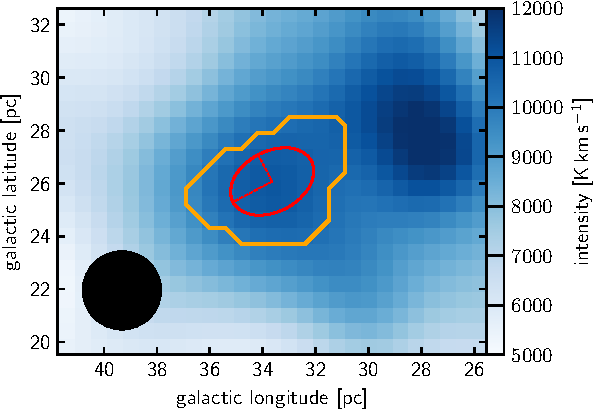
\includegraphics[width=0.6\linewidth]{images/chapters/papers/dendro/dendro_fig1}
    \caption[Example how \astrodendro assigns sizes to structures]{Example how \astrodendro assigns sizes to structures. The figure shows a random structure (\#4822) in the \co32 dataset of \ngc253 which contains a local emission peak. The total extent of the structure (orange) and the corresponding intensity-weighted second moment ellipse (red) are plotted on top of the total integrated intensity (0$^\mathrm{th}$ moment) \co32 map (blue). Dashed lines indicate the semi-major and semi-minor axes whereof the mean defines the size of the structure, here 1.20\,pc. The beam of 3\,pc FWHM is shown in the bottom left corner.
    Note that the background image shows all data to provide context whereas the size ellipse is calculated for the particular structure within the orange line.
    In this special case of a small structure, the algorithm described in Section~\ref{dendro: section: dendrogram size} assigns a size smaller than the beam to the structure. Nevertheless, the structure is resolved. Despite this effect, the \astrodendro definition of structure size has multiple advantages (cf. Appendix~\ref{appendix: dendro: size definition} for details).
    \label{dendro: figure: 1}}
\end{figure}

We define four properties from the dendrogram structures for our analysis:

\subsubsection{Size}
\label{dendro: section: dendrogram size}

We define the size $R$ of a structure as the arithmetic mean of the semi-major and semi-minor axis extent in position-position (PP) plane. The major and minor axes are defined by the projection of the PPV structure onto the PP plane, computed from the intensity weighted second moment in direction of greatest elongation in the PP plane. This definition is implemented in \astrodendro as the \texttt{radius} quantity.
In Appendix~\ref{appendix: dendro: size definition}, we explore the effect of different definitions of $R$ and conclude that it does not influence the derived size--line width relation considerably.

Note that \astrodendro parametrizes size as a semi axis (instead of full axis) which allows for resolved structures apparently smaller than the spatial resolution (given as FWHM). Furthermore, this definition incorporates intensity weighting and will thus assign sizes smaller than half the resolution to structures approaching to the resolution limit. The exact value depends on the distribution of emission within the structure. The chosen minimum PPV volume threshold in dendrogram ensures that a structure is resolved and derived sizes smaller than the resolution do \emph{not} mean that a structure is unresolved.
Figure~\ref{dendro: figure: 1} shows an example of a small but resolved structure in \co32 in \ngc253. The size inferred by the algorithm above is 1.20\,pc and thus less than half the FWHM beam size.
Note that we do not deconvolve the beam from the structure size and report the \astrodendro definition of size.


\subsubsection{Line width}
\label{dendro: section: dendrogram line width}

The velocity dispersion of a structure is defined as the intensity-weighted second moment (intensity-weighted velocity dispersion) over the pixels belonging to the structure as is implemented in \astrodendro as the \texttt{v\_rms} quantity.
Other definitions of line width can influence derived relations and can introduce artifacts as we test in Appendix~\ref{appendix: dendro: line width definition}.
We do not deconvolve the channel width from the obtained linewidths.
Note that projection effects can broaden the linewidth. Two clouds towards the same spatial position but separated along the line-of-sight may blend in velocity space and \astrodendro identifies them as a single structure. The linewidth of such a structure is broadened by the velocity difference between the constituent clouds which in turn depends on galactic dynamics, e.g. galactic rotation. 
Since the line width is derived on a per-pixel basis, bulk motions across the spatial extent of a structure do not influence the line width.


\subsubsection{Luminosity}
\label{dendro: section: luminosity}
We calculate the luminosity of each structure as the area integrated intensity $L = \int I \mathrm{d}A$ which translates to $L = \sum_i I_i \times A_\mathrm{pix}$ for discrete data with pixel area $A_\mathrm{pix}$. The integrated intensity $\sum_i I_i$ is reported directly by \astrodendro.


\subsubsection{Column density}
\label{dendro: section: dendrogram column density}

Following the typical approach in the literature, we define the column density $N$ of a structure as the number of H$_2$ atoms per effective area $A_\mathrm{eff}$.
The number of atoms per pixel $i$ is the product of CO-to-H$_2$ conversion factor $X_\mathrm{CO}$, flux $F_i$ and pixel area $A_\mathrm{pix}$, corrected for the line ratio in the case of \co32.
The effective area of a structure is defined as the luminosity--weighted ellipse area $A_\mathrm{eff} = n_\mathrm{pix}^\mathrm{eff} A_\mathrm{pix}$ with the effective number of pixels $n_\mathrm{pix}$. 
The area of a pixel $A_\mathrm{pix}$ cancels out and $N$ becomes:
\begin{equation}
    N_\mathrm{H_2} = \frac{\sum_i \frac{X_\mathrm{CO}}{r} F_i}{n_\mathrm{pix}^\mathrm{eff}}
    \label{equation: column density}
\end{equation}
We adopt standard \co10 conversion factors as listed in Table~\ref{dendro: table: conversion factors}.

To translate this to a \co32 conversion factor, we use the mean line ratio $r_{31} = I_{3-2}\,I_{1-0} ^{-1} = 0.67$.
The line ratios $r_{31}$ measured from the data convolved to the same resolution within the overlap area are $0.63$ in \ngc253 and $0.68$ in the GC. However, these measurements are poorly sampled due to the large \co10 beam (32\,pc) compared to the small overlap area defined by the \co32 field-of-view ($800\,\mathrm{pc} \times 400$\,pc). Also the line ratios outside the \co32 field-of-view cannot be measured from the data.
We therefore adopt a common line ratio of $r_{31}=0.67$ and note that other choices linearly scale the obtained column density.


\begin{table}
    \centering
    \begin{threeparttable}
        \caption[Gas mass conversion factors]{Conversion factors used in this analysis.
        \label{dendro: table: conversion factors}}
        
        \begin{tabular}{lccl}
            \toprule
            source & $X_\mathrm{CO}$ & $\alpha_\mathrm{CO}$ & Ref. \\
            & $\left[\frac{\mathrm{cm}^{-2}}{\mathrm{K\,km\,s}^{-1}}\right]$ & $\left[\frac{\mathrm{M}_\odot}{\mathrm{K\,km\,s}^{-1}\,\mathrm{pc}^2}\right]$ & \\[2mm]
            \midrule
\ngc253  & $0.5\times10^{20}$ & $1.1$ & L15, B13\\
GC      & $1.0\times10^{20}$ & $2.2$ & M99, Y03, B13\\
            \bottomrule
        \end{tabular}
        \tablenote{These conversion factors apply for \co10. We assume line ratios $r_{31} = I_{3-2}\,I_{1-0} ^{-1} = 0.67$ to correct higher excitation state of the \co32 lines.}
        \\
        \tablereference{L15 \citep{Leroy:2015ds}, B13 \citep{2013ARA&A..51..207B}, M99 \citep{1999A&A...341..256M}, Y03 \citep{2003ApJ...588..771Y}}
    \end{threeparttable}
\end{table}


\subsubsection{Mass}
\label{dendro: section: dendrogram mass}

The mass $M_\mathrm{struct}$ of a structure follows from the H$_2$ column density $N_\mathrm{struct}$  and the area $A_\mathrm{struct}$ as
\begin{equation}
    M_\mathrm{struct} = 1.36 \times 2\,\mathrm{u} \times N_\mathrm{struct} A_\mathrm{struct}
    \label{equation: mass}
\end{equation}
with the mass 2\,u (atomic unit $\mathrm{u}=1.66\times10^{-27}$\,kg) for a hydrogen molecule and the factor 1.36 corrects for the relative contribution of helium.
Note that this mass estimate traces the luminous mass (in contrast to the virial mass).


\subsubsection{Virial state}
\label{dendro: section: dendrogram virial state}

Molecular clouds are often assumed to be structures roughly in virial equilibrium \citep[e.g.][]{1987ApJ...319..730S} for which the deviation is expressed as the virial parameter $\avir = 2K / U$ where $K$ is the kinetic energy and $U$ the gravitational potential. Following \citet{2018ApJ...860..172S} for idealized spherical clouds, it is possible to relate its line width $\sigma$, virial parameter \avir, size $R$ and average column density $N$ (Eq.~\ref{equation: column density}) according to
\begin{equation}
    N = \frac{5}{f \avir G \pi} \frac{\sigma^2}{R},
\end{equation}
where $G$ is the gravitational constant, the factor $f = (1-\gamma/3)/(1-2\gamma/5)$ accounts for the internal cloud structure with a radial density profile $\rho(r) \propto r^{-\gamma}$. For $\gamma = 1$, thus $f = 10/9$.
This idealized case is certainly not correct for real molecular clouds but the deviation from an isolated self-gravitating cloud can reveal insight into its dynamic state and the contribution of other forces such as external pressure or magnetic support.

The effect of external pressure on the size--line width coefficient $\sigma^2/R$ has been worked out by \citet{2011MNRAS.416..710F} as
\begin{equation}
    \frac{\sigma^2}{R} = \frac{1}{3} \left( \pi \Gamma G \Sigma + \frac{4P_e}{\Sigma}\right)
\end{equation}
where $G$ is the gravitational constant, $\Sigma$ the mass column density and $P_e$ the external pressure. The form factor $\Gamma$ is $3/5$ for a spherical cloud of constant density or 0.73 for an isothermal spherical cloud of critical mass (used in the following). We include the contribution of helium to the mass and derive the mass column density $\Sigma = 1.36 \times 2\,\mathrm{u} \times N$ from the number column density $N$.


%%%%%%%%%%%%%%%%%%%%%%%%%%%%%%%%%%%%%%%%%%%%%%%%%%%%%%%%%%%%%%%%%%%%%%%%%%%%%%%%%%%%%%%%%%%%%%%%%%%%

\subsection{Binned analysis}
\label{dendro: section: binning}

The dendrogram analysis yields a very high number of structures, e.g. $\GTR 12,000$ individual structures in the \co32 data of \ngc253. As we are interested in the statistical properties of the clouds, we bin the structures in size bins of 0.1\,dex. Binning gives us the quantity of interest: the typical line width or luminosity at a fixed size scale, e.g. the scale of a molecular cloud ($\sim 10$\,pc) or a GMC ($\sim 100$\,pc). For each size bin, we report the median line width and the $16^{th}$ to $84^{th}$ percentile range as a measure of the line width spread. We exclude bins with less than three entries to get meaningful binned data. We further exclude the dendrogram trunks.
We explored various bin sizes and found 0.1\,dex to provide a good compromise between the number of bins and elements per bin.
For exploring the virial state of the gas in Section~\ref{dendro: section: virial state}, we apply the same binning approach with a bin size of 0.25\,dex. Since these data span a larger dynamical range, a larger bin size is optimal.

The minimum-volume-of-a-structure threshold imposes a diagonal cutoff in size-line width space.
We exclude the affected size interval from the analysis as listed in Table~\ref{dendro: table:  size limits}.
This effectively also excludes the smallest structures that are affected by beam convolution and channel convolution.
The corrections for beam convolution are $\LESS 25$\% even at the lower limits of sizes considered (Table~\ref{dendro: table:  size limits}). Given this we make no corrections.
As will be shown in Section~\ref{dendro: section: results}, the GC data is found at lower line width than the \ngc253 data, so the minimum-volume threshold affects the distribution starting at larger sizes in the GC. As a result the minimum recoverable size scale differs across sources although the datasets are at identical resolution.

We also cannot recover the largest size scales because they are dominated by galactic motions as explained in Section~\ref{dendro: section: dendrogram line width}. We find that the transition towards that regime is unexpectedly sharp and it is thus possible to remove affected structures based on a cut on size. Table~\ref{dendro: table:  size limits} shows the upper limits. They differ between sources but also depend on the (spatial and spectral) resolution of the data since coarser resolution creates more blending.

\begin{table}
    \centering
    \begin{threeparttable}
        \caption[Limits on recoverable structure sizes]{Limits on recoverable structure sizes.
        \label{dendro: table:  size limits}}
        
        \begin{tabular}{llcc}
            \toprule
            source & line & $R_\mathrm{min}$ & $R_\mathrm{max}$\\
                  &      & (1)              & (2)\\
            \midrule
\ngc253 & \co10 & 0.55 & 18\\
GC     & \co10 & 0.90 & 20\\
\ngc253 & \co32 & 6.0 & 60\\
GC     & \co32 & 8.5 & 68\\
            \bottomrule
        \end{tabular}
	    \tablenonote{(1) Completeness limit imposed by the minimum-volume-of-a-structure threshold.\\
        (2) Limit beyond which large scale dynamics (e.g. galactic rotation) dominate structure properties.
        }
    \end{threeparttable}
\end{table}


%%%%%%%%%%%%%%%%%%%%%%%%%%%%%%%%%%%%%%%%%%%%%%%%%%%%%%%%%%%%%%%%%%%%%%%%%%%%%%%%%%%%%%%%%%%%%%%%%%%%

\subsection{Fitting}
\label{dendro: section: fitting}

The size-binned size--line width and size--luminosity relations follow a power law and can be fitted with a weighted least squares minimization in logarithmic space. We report the square root of the diagonals of the covariance matrix as the errors for normalization $a$ and exponent $b$ as defined in Equation~\ref{equation: size-line width}. 
These statistical errors are often small as will be shown in the following Section~\ref{dendro: section: results} and systematic errors are non-negligible.

The normalization $a$ corresponds to the typical line width at a size scale of 1\,pc. Given the coarser resolution of the data, the line width at a scale of 10\,pc is a more meaningful measure of typical line width and we report this quantity as \sigmaten.
Similarly, for the size--luminosity relation we report \Lten as the typical luminosity of a 10\,pc sized structure instead of the normalization $c$.


%%%%%%%%%%%%%%%%%%%%%%%%%%%%%%%%%%%%%%%%%%%%%%%%%%%%%%%%%%%%%%%%%%%%%%%%%%%%%%%%%%%%%%%%%%%%%%%%%%%%
% RESULTS
%%%%%%%%%%%%%%%%%%%%%%%%%%%%%%%%%%%%%%%%%%%%%%%%%%%%%%%%%%%%%%%%%%%%%%%%%%%%%%%%%%%%%%%%%%%%%%%%%%%%

\section{Results}
\label{dendro: section: results}

In the following, we present the derived size--line width and size--luminosity relations as well as an analysis of the size--line width coefficient. For each of those analyses individually, we first present data on the GC and \ngc253 followed by a comparison.


%%%%%%%%%%%%%%%%%%%%%%%%%%%%%%%%%%%%%%%%%%%%%%%%%%%%%%%%%%%%%%%%%%%%%%%%%%%%%%%%%%%%%%%%%%%%%%%%%%%%

\subsection{Size -- line width relation}
\label{dendro: section: size line width}

Figure~\ref{dendro: figure: 2} presents the binned size--line width relation obtained as described in Section~\ref{dendro: section: structural analysis}. With the high resolution \co32 data, we are able to cover the size range down to $\LESS 1$\,pc whereas the lower resolution \co10 covers the larger scales up to $\sim 90$\,pc.
Details of the dendrogram statistics and power law fits to the size--line width relation are listed in Table~\ref{dendro: table: 2}.

\begin{figure}
    \centering
    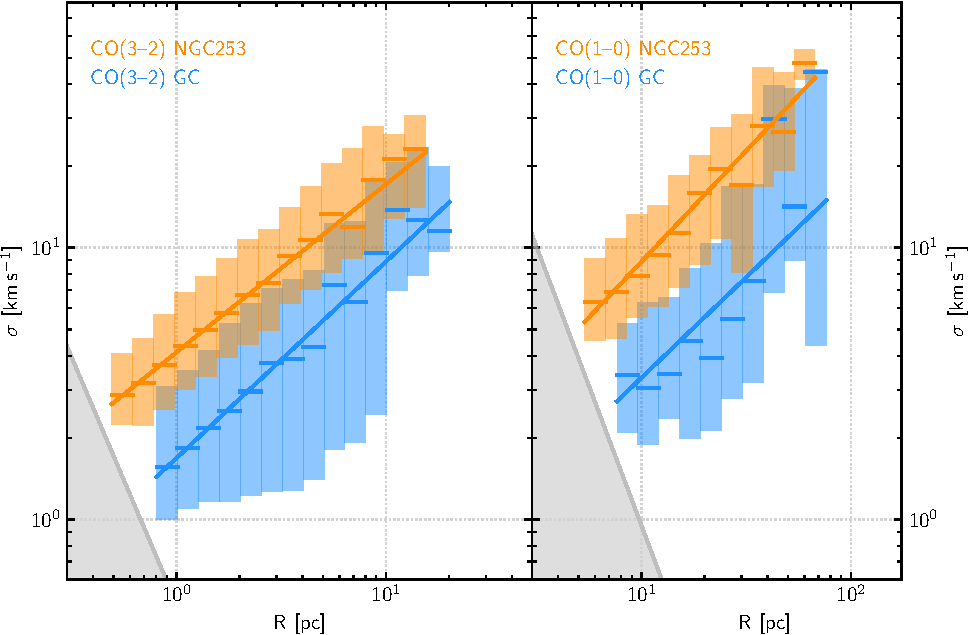
\includegraphics[width=\textwidth]{images/chapters/papers/dendro/dendro_fig2}
    \caption[Size--line width relation]{Binned size--line width relation for \co32 (\emph{left}) and \co10 (\emph{right}) in \ngc253 (orange) and the GC (blue). Horizontal lines indicate the median of the distribution of line widths (colored bars) in each bin. The values of the power law fits (solid lines) are given in Table~\ref{dendro: table: 2}. Grey, shaded areas indicate the minimum volume limit that ensures structures are significantly detected.
    The size--line width relation in \ngc253 is significantly offset towards larger line widths from the relation in the GC for both tracers.
    \label{dendro: figure: 2}}
\end{figure}


\begin{table}
    \centering
    \footnotesize
    \begin{threeparttable}
        \caption[Dendrogram statistics and fit results for size--line width and size--mass relations]{Dendrogram statistics and fit results for power law fits to the binned size--linewidth and size--luminosity relations shown in Figure~\ref{dendro: figure: 1} and \ref{dendro: figure: 3}.
        \label{dendro: table: 2}}
        
        \begin{tabular}{lcrrrcccc}
            \toprule
            source & line & \multicolumn{3}{c}{dendrogram structures} & \multicolumn{2}{c}{size--linewidth} & \multicolumn{2}{c}{size--luminosity}\\
            && total & branches & leaves & $b$ & \sigmaten & $d$ & log $\Lten$ \\
            &&&&& (1) & (2) & (3) & (4)\\
            \midrule
\ngc253 & CO(1--0) &   991 &  466 &  520 & $0.82\pm0.02$ & $ 8.9\pm0.2$ & $2.92\pm0.07$ & $4.27\pm0.11$ \\
GC     & CO(1--0) &   324 &  158 &  165 & $0.74\pm0.04$ & $ 3.3\pm0.4$ & $3.25\pm0.13$ & $4.34\pm0.20$ \\
\ngc253 & CO(3--2) & 12414 & 5145 & 7024 & $0.62\pm0.01$ & $17.1\pm0.1$ & $2.89\pm0.02$ & $5.44\pm0.03$ \\
GC     & CO(3--2) & 10235 & 4563 & 5570 & $0.72\pm0.03$ & $ 8.9\pm0.2$ & $2.69\pm0.02$ & $4.96\pm0.02$ \\
            \bottomrule
        \end{tabular}
	    \tablenonote{(1) Exponent $b$ of the power law fit to the size--linewidth relation according to Equation~\ref{equation: size-line width}.\\
        (2) Characteristic linewidth at 10\,pc according to the power law fit to the size--linewidth relation (Equation~\ref{equation: size-line width}) in \kms.\\
        (3) Exponent $d$ of the power law fit to the size--luminosity relation according to Equation~\ref{equation: size-luminosity}.\\
        (4) Characteristic luminosity at 10\,pc according to Equation~\ref{equation: size-luminosity} in $\log \mathrm{M}_\odot$.
        }
    \end{threeparttable}
\end{table}


%%%%%%%%%%%%%%%%%%%%%%%%%%%%%%%%%%%%%%%%%%%%%%%%%%%%%%%%%%%%%%%%%%%%%%%%%%%%%%%%%%%%%%%%%%%%%%%%%%%%

\subsubsection{Galactic Center}
\label{dendro: section: size line width: GC}

For the GC \co32, the binned data (Figure~\ref{dendro: figure: 2}, left) closely follow a power law. In \co10, the binned data (Figure~\ref{dendro: figure: 2}, right) scatter and do not follow a power law as closely as the \co32 does. The \co10 relation is less certain due to the low number of 324 recovered structures.
The power law fit according to Eq.~\ref{equation: size-line width} yields exponents of $b=0.72 \pm 0.03$ in \co32 and $b=0.74 \pm 0.04$ in \co10. 
The typical line width at 10\,pc derived from the fit is $\sigmaten = 8.9 \pm 0.2$\,\kms in \co32 and $\sigmaten = 3.3\pm0.9$\,\kms in \co10.

%%%%%%%%%%%%%%%%%%%%%%%%%%%%%%%%%%%%%%%%%%%%%%%%%%%%%%%%%%%%%%%%%%%%%%%%%%%%%%%%%%%%%%%%%%%%%%%%%%%%

\subsubsection{\ngc253}
\label{dendro: section: size line width: ngc253}

In \ngc253, the binned \co32 data (Figure~\ref{dendro: figure: 2}, left) almost perfectly follows a power law over more than one order of magnitude. In \co10, the statistical basis is weaker and the binned data (Figure~\ref{dendro: figure: 2}, right) shows a higher level of scatter than \co32 but the data still closely follows a power law relation.
A fit according to Eq.~\ref{equation: size-line width} results in exponents of $b=0.62 \pm 0.01$ in \co32 and $b=0.82 \pm 0.02$ in \co10. 
The fit yields typical line widths at 10\,pc of $\sigmaten = 17.1 \pm 0.1$\,\kms in \co32 and $\sigmaten = 8.9 \pm 0.2$\,\kms in \co10.

%%%%%%%%%%%%%%%%%%%%%%%%%%%%%%%%%%%%%%%%%%%%%%%%%%%%%%%%%%%%%%%%%%%%%%%%%%%%%%%%%%%%%%%%%%%%%%%%%%%%

\subsubsection{Comparison of the size -- line width relations}
\label{dendro: section: size line width: comparison}

The size--line width relations in the GC and \ngc253 are significantly offset from each other at similar slopes. In both cases, \co10 and \co32, the GC size--line width relation is offset towards smaller line widths compared to \ngc253. The line widths are wider in \ngc253 by a factor $\sim 1.9$ and $\sim 2.7$ for \co32 and \co10, respectively. Parametrized as \sigmaten (cf. Section~\ref{dendro: section: fitting}), the GC shows consistently smaller line widths by 8.2\,\kms (\co32) and 5.6\,\kms (\co10). In both \co10 and \co32, the offset is roughly constant across size, i.e. the line width ratio between \ngc253 and the GC is constant.
As mentioned in Section~\ref{dendro: section: size line width: GC}, the lower number of structures potentially affects the power law fit to the \co10 GC data. However, even if so, Figure~\ref{dendro: figure: 2} (right) consistently shows significantly smaller line widths\footnote{This also applies to the unbinned data.} than in \ngc253.

It is also noteworthy that the GC shows a wider distribution of line widths than \ngc253 at a fixed size scale. This implies a greater variation of turbulent cloud properties in the GC and more uniform clouds in \ngc253.

When comparing the two CO lines in each galaxy center, the line widths at $8-16$\,pc scales do not match but the \co32 lines are wider. In \ngc253, this difference is $\sim 8$\,\kms (factor $\sim 1.9$) and $\sim 6$\,\kms (factor $\sim 2.7$) in the GC.
This is opposite to the expectation that \co10 should trace larger and more diffuse structures with greater turbulent motions and thus line widths.

The reason for the observation of lower line widths in \co10 is about equal parts the change in image resolution and tracer properties of the CO lines. As a test, we degrade the resolution of the \co32 data in \ngc253 losing the ability to probe size scales $\LESS 10$\,pc and redo the dendrogram analysis. Degrading the spatial (6.4\,pc to 32\,pc in ten steps to match the \co10 data) and spectral (2.5\,\kms to 5.0\,\kms) resolution causes a shift of the size--line width relation towards larger sizes (to the right-hand side in Figure~\ref{dendro: figure: 2}) approximately linear with resolution. At a fixed size scale, the measured line width is thus smaller with lower resolution data. Half of the observed line width mismatch is explained directly as a consequence of these resolution effects. 
The other half is related to the tracer properties of the CO lines and specifics of the dendrogram algorithm\footnote{A large structure can include multiple peaks (smaller substructures) along the line-of-sight. Due to excitation with $r_{31}\LESS 1$ the gas in between the peaks is fainter in \co32 than \co10. The linewidth derived as the intensity-weighted second moment is thus smaller for the \co10 structure. The same effect causes the linewidth to increase when decreasing the resolution as emission is spread out spatially. The impact of this effect on a given structure depends greatly on the specific configuration and excitation. Trunks as the largest structures are strongly affected but typically, the nested substructure splits rapidly (the dendrogram tree branch out quickly after the trunk level) and thus the effect quickly becomes negligible towards nested structures.}.
As we are interested in the comparison across environment (\ngc253 vs. GC), we will not discuss this effect further.


%%%%%%%%%%%%%%%%%%%%%%%%%%%%%%%%%%%%%%%%%%%%%%%%%%%%%%%%%%%%%%%%%%%%%%%%%%%%%%%%%%%%%%%%%%%%%%%%%%%%

\subsection{Size -- luminosity relation}
\label{dendro: section: size luminosity}

\begin{figure}
    \centering
    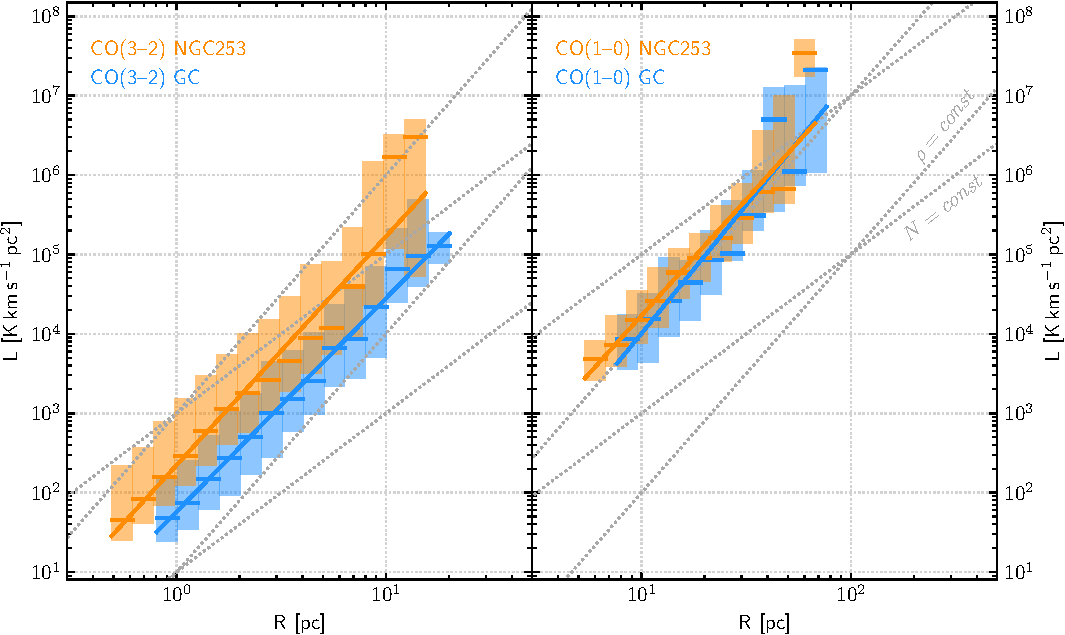
\includegraphics[width=\textwidth]{images/chapters/papers/dendro/dendro_fig3}
    \caption[Size--luminosity relation]{Relation between dendrogram structure size and luminosity for \co32 (\emph{left}) and \co10 (\emph{right}) in \ngc253 and the GC. Horizontal lines indicate the median of the distribution of luminosities (colored bars) in each bin. The values of the power law fits (solid lines) are given in Table~\ref{dendro: table: 2}.
    In each panel, two lines of constant surface density $N$ ($M \propto L \propto R^2$) and constant volume density $\rho$ ($M \propto L \propto R^3$) are shown for reference.
    }
    \label{dendro: figure: 3}
\end{figure}

Figure~\ref{dendro: figure: 3} shows the size--luminosity relation and Table~\ref{dendro: table: 2} lists the power law fit parameters according to Equation~\ref{equation: size-luminosity}.
In Appendix~\ref{appendix: dendro: size mass}, we also show the size--mass relation after applying the conversion factors listed in Table~\ref{dendro: table: conversion factors} to Figure~\ref{dendro: figure: 3}.


%%%%%%%%%%%%%%%%%%%%%%%%%%%%%%%%%%%%%%%%%%%%%%%%%%%%%%%%%%%%%%%%%%%%%%%%%%%%%%%%%%%%%%%%%%%%%%%%%%%%

\subsubsection{Galactic Center}
\label{dendro: section: size luminosity: GC}

The binned size--luminosity relations for \co10 and \co32 in the GC scale very close to power laws.
The fits yield power law exponents of $d=2.69 \pm 0.02$ in \co32 and $d=3.25 \pm 0.13$ in \co10.
The high slope in \co10 is influenced by the last bin ($R\sim80$\,pc). Without this bin, the slope is consistent with a more moderate $d=3$.
A power law exponent $\LESS 3$ in \co32 implies decreasing volume density for large size structures whereas the higher exponent $\GTR 3$ in \co10 indicates increasing volume density with size. Note, however, that the \co10 relation is less certain due to the low number of 324 recovered structures.

%%%%%%%%%%%%%%%%%%%%%%%%%%%%%%%%%%%%%%%%%%%%%%%%%%%%%%%%%%%%%%%%%%%%%%%%%%%%%%%%%%%%%%%%%%%%%%%%%%%%

\subsubsection{\ngc253}
\label{dendro: section: size luminosity: ngc253}

In \ngc253, the binned size--luminosity relations also scale nearly perfectly as power laws.
Although we remove the dendrogram trunks and large scale structures affected by galactic dynamics, the largest size scale bins in Figure~\ref{dendro: figure: 3} are still somewhat affected as can be seen by the sudden upturn of the relations. However, this only negligibly affects the power law fits which yield exponents of $d=2.89 \pm 0.02$ in \co32 and $d=2.92 \pm 0.07$ in \co10.
These exponents $d \sim 3$ imply approximately constant volume density independent of the structure size.

%%%%%%%%%%%%%%%%%%%%%%%%%%%%%%%%%%%%%%%%%%%%%%%%%%%%%%%%%%%%%%%%%%%%%%%%%%%%%%%%%%%%%%%%%%%%%%%%%%%%

\subsubsection{Comparison of the size -- luminosity relation}
\label{dendro: section: size luminosity: comparison}

Figure~\ref{dendro: figure: 3} shows that there is little difference in the size--luminosity relations between \ngc253 and the GC.
In \co10, the relations are almost identical within the scatter. The \co32 size--luminosity relations are offset by a factor $\sim 2-3$ with higher luminosities in \ngc253. 
Taken together this implies higher excitation in \ngc253.
Higher luminosities in \ngc253 than in the GC are expected since the former is known to be more massive and brighter.

The size--mass relations (Appendix~\ref{appendix: dendro: size mass}) that follow from Figure~\ref{dendro: figure: 3} after applying the conversion factors listed in Table~\ref{dendro: table: conversion factors} eliminate the luminosity offset in \co32 between \ngc253 and the GC. In \co10, the sources remain very close in their size--mass relation.

Reflecting the data, the power law fits are similar as well. In \co32, the exponents are identical within the errors while for \co10 the exponents differ by $\sim10$\%. Within the distribution of the data (indicated by the bars in Figure~\ref{dendro: figure: 3}), exponents deviating systematically by up to 20\% from the best fit are plausible.
In \co10, the power law normalisations \Lten of GC and \ngc253 are consistent but significantly smaller than for \co32.
As for the size--line width relation, the two CO tracers do not match at the overlapping size scale of $8-16$\,pc. This is caused by the differing resolutions and tracer properties (cf. Section~\ref{dendro: section: size line width: comparison}).

In addition to the similar size--luminosity relations, we further conclude that there is no significant difference in the density and mass structures between \ngc253 and the GC by comparing the column density, volume density and mass probability distribution functions (PDFs). Appendix~\ref{appendix: dendro: mass density structure} shows these PDFs and discusses their properties.


%%%%%%%%%%%%%%%%%%%%%%%%%%%%%%%%%%%%%%%%%%%%%%%%%%%%%%%%%%%%%%%%%%%%%%%%%%%%%%%%%%%%%%%%%%%%%%%%%%%%

\subsection{Virial state of the molecular gas}
\label{dendro: section: virial state}

In order to explore the origin of the differing size--line width relations in \ngc253 and the GC, we now examine the virial state (Section~\ref{dendro: section: dendrogram virial state}) of the obtained structures. This analysis assumes that the luminous mass (Section~\ref{dendro: section: dendrogram mass}) derived from CO is a good mass estimate and explores the dynamical state of the structures implied by the size--line width relations (Section~\ref{dendro: section: size line width}).

\begin{figure}[t]
    \centering
    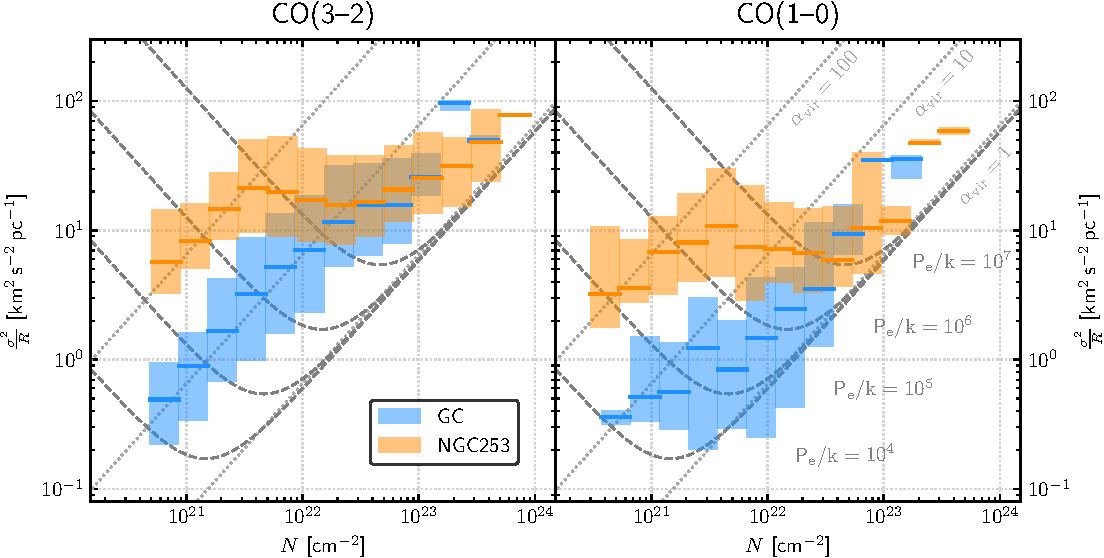
\includegraphics[width=\textwidth]{images/chapters/papers/dendro/dendro_fig4}
    \caption[Size--line width coefficient vs. column density relation]{Size--line width coefficient as a function of column density in \ngc253 and the GC under the assumption that luminous (CO detected) mass traces virial (gravitational) mass. Diagonal lines indicate lines of constant virial parameter under the assumption of spherical clouds (cf. Section~\ref{dendro: section: virial state}). V-shaped lines represent lines of constant external pressure on an idealized spherical cloud (cf. Section~\ref{dendro: section: virial state}). Horizontal lines indicate the median of the distribution of $\Sigma^2/R$ (colored bars) in each bin. \emph{left}: low resolution \co10; \emph{right}: high resolution \co32. 
    Note that the derived column density should be considered a lower limit (cf. Section~\ref{dendro: section: physical implications}). A different choice of conversion factors shifts the obtained relations along the x-axis but does not influence the slope.
    Due to the similar geometry and gas distribution in \ngc253 and the GC, a relative comparison is still possible even if the absolute values must be interpreted with care. The strongly enhanced $\sigma^2/R$ at column densities $N \LESSSIM 3 \times 10^{22}$\,\sqcm implies that the low column density molecular gas in \ngc253 is gravitationally unbound which is not the case in the GC. Appendix~\ref{appendix: dendro: virial state separated} shows this plot separated in size bins to address the degeneracy between $\sigma$ and $R$ in the size--line width coefficient.
    }
    \label{dendro: figure: 4}
\end{figure}

Figure~\ref{dendro: figure: 4} shows the $\sigma^2/R$ (size--line width coefficient) versus column density $N$ relation. For reference, Figure~\ref{dendro: figure: 4} shows lines of constant virial parameter at $\avir = 1, 10, 100$ and lines of constant external pressure at $P_e = 10^4, 10^5, 10^6, 10^7$\,K\,\pcm3.

For the interpretation of Figure~\ref{dendro: figure: 4}, it must be kept in mind what a dendrogram structure is (cf. Section~\ref{dendro: section: structural analysis}): a data parametrization that does not necessarily correspond to the simplistic idea of a cloud as an independent entity.
Care must thus be taken when trying to interpret Figure~\ref{dendro: figure: 4} as the virial state of clouds of a certain size.
Especially on scales of a few parsecs, this figure shows the dependence of $\sigma^2/R$ on $N$ for substructures within larger objects rather than ``clouds''. On such small size scales other contributions to the line width like internal motions and pressure must be taken into account. Hence, a comparison with the theoretical lines for virial parameter and external pressure can not be interpreted to yield absolute values but indicate qualitative and relative differences.

Figure~\ref{dendro: figure: 4} shows all data regardless of size or line width. The size--line width coefficient $\sigma^2/R$ is thus degenerate between size and line width. Separating Figure~\ref{dendro: figure: 4} by size or line width does not change the picture, though, as we show in Appendix~\ref{appendix: dendro: virial state separated}. The relations seen in Figure~\ref{dendro: figure: 4} also hold when separating by structure size (Figure~\ref{dendro: figure: D}).


%%%%%%%%%%%%%%%%%%%%%%%%%%%%%%%%%%%%%%%%%%%%%%%%%%%%%%%%%%%%%%%%%%%%%%%%%%%%%%%%%%%%%%%%%%%%%%%%%%%%

\subsubsection{Galactic Center}
\label{dendro: section: size virial state: GC}

Figure~\ref{dendro: figure: 4} (right) shows that for \co10, $\sigma^2/R$ scales with column density approximately as a power law with unity exponent, i.e. at constant virial parameter.
The \co32 data (Figure~\ref{dendro: figure: 4}, left) also follows a power law scaling with column density but at an overall higher virial parameter ($\alpha \sim 10$) than \co10 ($\alpha \sim3-10$).

%%%%%%%%%%%%%%%%%%%%%%%%%%%%%%%%%%%%%%%%%%%%%%%%%%%%%%%%%%%%%%%%%%%%%%%%%%%%%%%%%%%%%%%%%%%%%%%%%%%%

\subsubsection{\ngc253}
\label{dendro: section: size virial state: ngc253}

For \ngc253, both \co10 and \co32 show a more complicated relation between $\sigma^2/R$ and column density.
Towards high column densities of $N \GTRSIM 3 \times 10^{22}$\,\sqcm and low column densities of $N \LESSSIM 3 \times 10^{21}$\,\sqcm the data suggests a power law scaling roughly consistent with a constant virial parameter.
At high column densities, the virial parameters are therefore significantly lower ($\alpha \sim 2-10$) than in the low column density regime ($\alpha \sim 100$).
In the intermediate range of $3 \times 10^{22}\,\mathrm{cm}^{-2} \GTRSIM N \GTRSIM 3 \times 10^{21}$\,\sqcm, the size--line width coefficient is approximately constant and the medians even temporarily decreases with increasing column density. The hint towards a local dip in $\sigma^2/R$ for \co10 falls on the minimum of the constant pressure line with $P_e \sim 10^7$\,K\,\pcm3 and for \co32 the local dip corresponds to $P_e \sim 10^{7.5}$\,K\,\pcm3. This implies high external pressures in the center of \ngc253.


%%%%%%%%%%%%%%%%%%%%%%%%%%%%%%%%%%%%%%%%%%%%%%%%%%%%%%%%%%%%%%%%%%%%%%%%%%%%%%%%%%%%%%%%%%%%%%%%%%%%

\subsubsection{Comparison of the virial state}
\label{dendro: section: size virial state: comparison}

\ngc253 and the GC behave very differently in $\sigma^2/R$--$N$ space. 
In both \co10 and \co32, the Galactic Center structures scale with decreasing $\sigma^2/R$ towards lower column density at roughly constant virial parameter.
For the \ngc253 structures, however, a potential power law scaling is broken at intermediate column densities. This causes the relations in \ngc253 to deviate from the GC relations at $N \LESSSIM 3 \times 10^{22}$\,\sqcm. At $N \GTRSIM 3 \times 10^{22}$\,\sqcm no significant difference between \ngc253 and the GC is apparent and structures in both sources are found at low virial parameters of a few.


%%%%%%%%%%%%%%%%%%%%%%%%%%%%%%%%%%%%%%%%%%%%%%%%%%%%%%%%%%%%%%%%%%%%%%%%%%%%%%%%%%%%%%%%%%%%%%%%%%%%
% DISCUSSION
%%%%%%%%%%%%%%%%%%%%%%%%%%%%%%%%%%%%%%%%%%%%%%%%%%%%%%%%%%%%%%%%%%%%%%%%%%%%%%%%%%%%%%%%%%%%%%%%%%%%

\section{Discussion}
\label{dendro: section: discussion}

%%%%%%%%%%%%%%%%%%%%%%%%%%%%%%%%%%%%%%%%%%%%%%%%%%%%%%%%%%%%%%%%%%%%%%%%%%%%%%%%%%%%%%%%%%%%%%%%%%%%

\subsection{Comparison to the literature}
\label{dendro: section: literature}

We now compare our results to the vast body of literature work on scaling relations in various environments within and outside of the Milky Way.

There are different effects that either increase or reduce the observed exponents of the scaling relations depending on specific details of the used cloud identification algorithm and the unknown exact geometry along the line-of-sight towards the source.
The simulations by \citet{2010ApJ...712.1049S} show that the intrinsic size--linewidth exponents can be even steeper than the exponent retrieved from position-position-velocity (PPV) data. This happens because the PPV analysis can split up large clouds into several smaller structures due to intrinsic velocity gradients along the line-of-sight.
On the other hand, the intrinsic exponent may be more shallow than an observed exponent due to line-of-sight contamination by low levels of unrelated emission at similar velocities \citep{2019MNRAS.490.2648B}. Such contamination more often affects farther away and larger clouds and thus steepens the exponent.
This is the same effect as we observe for the largest structures (Section~\ref{dendro: section: dendrogram line width}).

Hence, differences in the source orientation and tracer properties may significantly influence the obtained size--linewidth and size--luminosity exponents and comparisons across the literature have to be considered carefully.


%%%%%%%%%%%%%%%%%%%%%%%%%%%%%%%%%%%%%%%%%%%%%%%%%%%%%%%%%%%%%%%%%%%%%%%%%%%%%%%%%%%%%%%%%%%%%%%%%%%%

\subsubsection{Size--line width relation}
\label{dendro: section: literature: size line width}

\begin{figure}[t]
    \centering
    \includegraphics[width=0.6\linewidth]{images/chapters/papers/dendro/dendro_fig5}
    \caption[Literature comparison: size--line width exponent]{The size--line width exponent $b$ as in $\sigma \propto R^b$ derived in this work compared to Galactic and extra-galactic literature. Molecular tracers are colorcoded in shades of blue for Galactic measurements and shades of orange for extra-galactic measurements. The shown studies vary strongly in the size scale over which the exponent $b$ was derived from $\LESS 1$\,pc to $\sim 200$\,pc. See Section~\ref{dendro: section: literature: size line width} for details. The abbreviated references refer to (ordered left to right): S+87 \citep{1987ApJ...319..730S}, MD+17 \citep{2017ApJ...834...57M}, R+19 \citep{2019A&A...632A..58R}, R+16 \citep{2016ApJ...822...52R}, S+16 \citep{Storm:2016cl}, K+17 \citep{2017A&A...603A..89K}, S+12 \citep{2012MNRAS.425..720S}, W+19 \citep{2019ApJ...885...50W}, N+16 \citep{2016ApJ...831...32N}, B+08 \citep{Bolatto:2008iv} and F+18 \citep{2018ApJ...857...19F}.}
    \label{dendro: figure: 5}
\end{figure}

Figure~\ref{dendro: figure: 5} shows an overview of the literature including our new measurements that we will discuss in the following.
We find $b=0.65 \pm 0.01$ (\co32, \ngc253), $b=0.72 \pm 0.03$ (\co32, GC) as well as $b=0.82 \pm 0.02$ (\co10, \ngc253) and $b=0.74\pm0.04$ (\co10, GC).
In the GC, \citet{2012MNRAS.425..720S} found $b=0.62-0.79$ for dense gas tracers (N$_2$H$^+$, HCN, H$^{13}$CN, HCO$^+$) where $b$ spans Bayesian 95\% highest density intervals (95\%HDI) of $0.2-1.6$ (equivalent to $2\sigma$ errors in the case of Gaussian distributions). Their error interval is thus approximately twice as large compared to the usual $1\sigma$ intervals. Further observations by \citet{2017A&A...603A..89K} confirm the steep relation in the GC $b=0.66\pm0.18$ using N$_2$H$^+$. Both of these studies cover size scales up to $\sim 40$\,pc \citep{2012MNRAS.425..720S} and $\sim 8$\,pc \citep{2017A&A...603A..89K} and are thus consistent with our results in both the GC and \ngc253.
\citet{2017ApJ...834...57M} found $b=0.63 \pm 0.30$ for $\GTR 8000$ $^{12}$CO(1--0) clouds in the Galactic plane \citep[using the][survey]{2001ApJ...547..792D} on size scales $\LESS 1$\,pc to $\GTRSIM 200$\,pc which is confirmed by \citet{2019A&A...632A..58R} with $b=0.63\pm0.03$ for $^{13}$\co32. Using the same \co10 data, \citep{2016ApJ...822...52R} did a dendrogram analysis for the inner and outer galaxy separately resulting in $b=0.52\pm0.03$ (inner galaxy) and $b=0.49\pm0.04$ (outer galaxy). They also find a significantly higher normalization in the inner galaxy (corresponding to $\sigmaten = 1.65\pm0.20$\,\kms and $\sigmaten = 1.17\pm0.19$\,\kms for inner and outer galaxy, respectively) indicating pressure confinement of clouds in the inner galaxy. This is lower than our result of $\sigmaten = 3.3\pm0.4$\,\kms for \co10 in the GC implying that the GC is a region of broader line widths within the inner galaxy.
Star formation regions in the Milky Way outside the GC typically exhibit $b\sim 0.5-0.7$ \citep[e.g.][]{1987ApJ...319..730S,Storm:2016cl} across a wide range of covered size scales ($\LESS 0.1$\,pc to $\LESSSIM 100$\,pc in these studies).

In the LMC, \citet{2019ApJ...885...50W} find a combined $b=0.64$ in $^{12}$CO(1--0) and $b=0.59$ in $^{13}$CO(1--0) with significant scatter across the six mapped regions ($b=0.32-0.97$ and $b=0.36-1.00$ for $^{12}$CO and $^{13}$CO, respectively). They find $b=0.60\pm0.03$ ($^{12}$CO) and $b=0.43\pm0.08$ ($^{13}$CO) for the high-mass star forming region 30~Doradus similar to e.g. \citet{2016ApJ...831...32N} with $b=0.65\pm0.04$ ($^{12}$\co21). These studies in the LMC also cover small size scales of $3-15$\,pc \citep{2019ApJ...885...50W} and $0.15-5$\,pc \citep{2016ApJ...831...32N}. Across the disks of nearby galaxies comparable values have been obtained on GMC scales at $\GTRSIM 30-50$\,pc resolution (e.g. $b=0.60\pm0.60$ \citealt{Bolatto:2008iv}; $b=0.48\pm0.05$, NGC300, \citealt{2018ApJ...857...19F}).

\citet{Wong:2017hx} note a striking deviation in the size--line width normalization of factor of $\sim 5$ between the quiescent Planck cold cloud and the star formation region 30~Doradus. Consistent across $^{12}$CO and $^{13}$CO, they conclude that this difference is unlikely to be caused by optical depth. The enhanced line width in the star formation region relative to a quiescent region is qualitatively consistent with our observation of the factor $1.9-2.7$ enhancement in \ngc253 relative to the GC.

Our new measurements of the size--line width exponent in \ngc253 are therefore consistent with previous studies in the Galactic Center and star forming galaxies. The measurements in the GC are also compatible with previous measurements in the same region, albeit with different tracers.


%%%%%%%%%%%%%%%%%%%%%%%%%%%%%%%%%%%%%%%%%%%%%%%%%%%%%%%%%%%%%%%%%%%%%%%%%%%%%%%%%%%%%%%%%%%%%%%%%%%%

\subsubsection{Size -- luminosity (mass) relation}
\label{dendro: section: literature: size mass}

\begin{figure}[t]
    \centering
    \includegraphics[width=0.6\linewidth]{images/chapters/papers/dendro/dendro_fig6}
    \caption[Literature comparison: size--luminosity exponent]{The size--luminosity (mass) exponent $d$ as in $L \propto R^d$ (or $m \propto R^d$) derived in this work compared to Galactic and extra-galactic literature. Molecular tracers are colorcoded in shades of blue for Galactic measurements and shades of orange for extra-galactic measurements. The shown studies vary strongly in the size scale over which the exponent $d$ was derived from $\LESS 1$\,pc to $\sim 200$\,pc. See Section~\ref{dendro: section: literature: size mass} for details. The abbreviated references refer to (ordered left to right): MD+17 \citep{2017ApJ...834...57M}, C+19 \citep{2019MNRAS.483.4291C}, R+19 \citep{2019A&A...632A..58R}, B+08 \citep{Bolatto:2008iv}, W+17 \citep{Wong:2017hx}, C+14 \citep[cf. definitions of the regions within M51]{2014ApJ...784....3C}, F+18 \citep{2018ApJ...857...19F}, S+17 \citep{2017A&A...608A..98S}.}
    \label{dendro: figure: 6}
\end{figure}

We derive steep size--luminosity relations with power law exponents $d\sim3$. In the GC, \co10 yields the steepest exponent at $d=3.25\pm0.13$ while the exponent derived from \co32 is more shallow at $d=2.69\pm0.02$. The results for \ngc253 are consistent at $d=2.92\pm0.07$ (\co10) and $d=2.89\pm0.02$ (\co32).

Figure~\ref{dendro: figure: 6} gives an overview of the size--mass exponent found in this study and in the literature which is discussed in the following.
\citet{2017ApJ...834...57M}, using the \citet{2001ApJ...547..792D} Galactic plane CO data, obtained a power law exponent $d=2.2 \pm 0.2$ for $\GTR 8000$ clouds in the Galactic plane.
In the Milky Way first quadrant (using the COHRS \co32 data, \citealt{2013ApJS..209....8D}), \citet{2019MNRAS.483.4291C} find $d=2.26\pm0.06$ in their sample of $\GTR 85000$ disk clouds and $d=2.17\pm0.38$ in the subsample with good distance estimates.
Very similar results are found by \citet{2019A&A...632A..58R} using the CHIMPS \co32 data with $d=2.26\pm0.02$ (full sample) and $d=2.42\pm0.05$ (distance $8-12$\,kpc) for disk clouds.
No size--luminosity or size--mass relations across a collection of clouds are reported in the literature for the GC yet\footnote{\citet{2017A&A...603A..90K} report exponents of $d\sim1$ and $d\sim1.7$ within six selected clouds in the GC. Their derivation of the exponent from two observations of different resolution strongly differs from data segmentation approaches like dendrograms.}

Steeper exponents $d \GTRSIM 2.5$ are commonly encountered in nearby extra-galactic studies on GMC size scales \citep[$\GTRSIM 50$\,pc, e.g.][]{Bolatto:2008iv}. The environment plays a role for the obtained exponent as shown by \citet{2014ApJ...784....3C} in M51 where $d$ varies from 1.5 to 2 to 2.5 for inter-arm, inner galaxy and spiral arm regions for $\sim 40$\,pc resolution. 
In the LMC, \citep{Wong:2017hx} find $d=2.52\pm0.05$ and $d=3.10\pm0.11$ for the two special environments of the Planck cold cloud and 30~Doradus, respectively, on small size scales of $\sim 0.3 - 10$\,pc.
Relatively shallow exponents are found in NGC300 at 10\,pc scale resolution with $d=2.00\pm0.12$ \citep{2018ApJ...857...19F}.
In special environments, the size--mass relation can deviate from these values. The northern filament in Centaurus A which shows signs of recent star formation has a steeper size--mass relation of order $d \sim 3-4$ as implied by the analysis of \citet{2017ApJ...834...57M}.

The literature agrees upon an environment dependence of $d$ as well as the importance of geometrical effects. However, there is disagreement about how significant the change in the derived exponent $d$ is, especially given that most data are at low resolution and the (extragalactic) sample sizes tend to be small. Nonetheless,exponents $d \sim 3$ as we derive are among the steepest found so far. Our results strengthen the previous findings that galactic centers are a special environment with steeper size--luminosity (mass) relations.


%%%%%%%%%%%%%%%%%%%%%%%%%%%%%%%%%%%%%%%%%%%%%%%%%%%%%%%%%%%%%%%%%%%%%%%%%%%%%%%%%%%%%%%%%%%%%%%%%%%

\subsubsection{Virial state of the molecular gas}
\label{dendro: section: literature: virial state}

A power law scaling between $\sigma^2/R$ and surface or column density is expected from the theoretical arguments in Section~\ref{dendro: section: virial state} and reported in the literature.
\citet{Heyer:2009ii} found $N \propto (\sigma^2/R)^{0.6}$ for Giant Molecular Clouds in the Milky Way using data from the Galactic Ring Survey \citep[GRS, ][]{2006ApJS..163..145J}. \citet{2016ApJ...831...32N} find a steeper slope at $N \propto (\sigma^2/R)^{0.90 \pm 0.12}$ in 30~Doradus in the LMC. 
This is consistent with our results of the GC (In Figure~\ref{dendro: figure: 4}, the lines of constant virial parameter are of slope 1.).
The approximately constant $\sigma^2/R$ in the intermediate column density regime ($3 \times 10^{22}\,\mathrm{cm}^{-2} \GTRSIM N \GTRSIM 3 \times 10^{21}$\,\sqcm) for our \ngc253 data (Figure~\ref{dendro: figure: 4}), however, is not noted in the literature.

Molecular clouds in the disks of the Milky Way and nearby galaxies are typically found to be gravitationally bound at virial parameters of a few\footnote{Note that depending on the definition of the virial parameter $\avir=1$ or $\avir=2$ can denote boundness.} (e.g. Galactic disk \citealt{2006ApJS..163..145J}; NGC300, \citealt{2014ApJ...784....3C}; M51, \citealt{2018ApJ...857...19F}). 
The derivation of column density differs strongly in the literature (tracers, definition of size and area) which directly reflects on the virial parameter. Any comparison must therefore be considered carefully.
We work with CO whose lowest rotational transitions are not a very good column density tracer because it becomes optically thick easily at typical GMC column densities. For the warm and dense conditions in \ngc253 and the GC, CO line emission reaches opacities in the moderately optically thick regime of order $\tau = 1-10$ at parsec to tens of parsecs scale resolution (\ngc253: e.g. \citealt{2018ApJ...867..111Z,2015ApJ...801...63M,2004ApJ...611..835P}; GC: e.g. \citealt{2017MNRAS.471.2523Y,2014A&A...570A..65G,1998A&A...331..959D}). 
From these studies, no systematic deviation between the CO optical depths in \ngc253 and the GC is expected and complicating effects such as opacity broadening \citep{Hacar:2016gu} should apply equally.
The conversion factors in principle already account for optical depth but likely underestimate the effect. The conversion factors are averages for the respective environments whereas our analysis targets mainly dense subregions within, that may be characterized by higher conversion factors.
The derived column densities should thus be understood as a lower limit and consequently the virial parameters as an upper limit.

Enhanced virial parameters relative to the disk are expected and observed for galactic centers and starbursts due to the effect of the galaxy potential, the large amount of dense molecular gas and external pressure present in such environments \citep[e.g.][]{2018ApJ...860..172S,2018ApJ...854..100M}.
Therefore, $\avir \GTRSIM 10$ in the GC and the high column density regime in \ngc253 matches the expectation from the literature when considering gas tracer and environment.
Higher virial parameters up to $\avir \GTR 100$ in the lower column density regime in \ngc253 exceed the parameter range that is compatible with (marginally) bound gas even for extreme conditions. Instead, such high virial parameters can only be interpreted as to indicate unbound (non-selfgravitating) gas.


%%%%%%%%%%%%%%%%%%%%%%%%%%%%%%%%%%%%%%%%%%%%%%%%%%%%%%%%%%%%%%%%%%%%%%%%%%%%%%%%%%%%%%%%%%%%%%%%%%%%

\subsection{Physical Implications}
\label{dendro: section: physical implications}

For the following interpretation of the data shown in Section~\ref{dendro: section: results} it must be kept in mind that a dendrogram structure does not necessarily correspond to a molecular cloud as a physical entity (cf. Section~\ref{dendro: section: structural analysis}). Instead, most structures correspond to a certain level of substructure within a GMC. Statements about individual molecular clouds are thus not meaningful but it is possible to infer statistical properties of coherent gas parcels on a given size scale, for a given mass or other properties.

% size line width
Section~\ref{dendro: section: size line width} shows that the line widths in \ngc253 are enhanced relative to the GC across size scales. The difference is large with a factor $\sim 1.9$ in \co32 and a factor $\sim 2.7$ in \co10. At a reference scale of 10\,pc the difference is $\sim 6-8$\,\kms depending on the tracer.
This difference is not due to different large scale motions (e.g. galactic rotation) 
since we exclude the structures that are noticeably affected (Section~\ref{dendro: section: binning}).
In principle, the enhanced line width could be due to differences in the mass or density structure of molecular clouds.
Clouds in \ngc253 could be more dense, thus more massive and more luminous for a given size, and supported by a higher turbulent pressure than a cloud of the same size in the GC.
% size--luminosity
This possibility is ruled out in Section~\ref{dendro: section: size luminosity} which shows that the size--luminosity relations in \ngc253 and the GC are similar. Most importantly, the power law scaling (exponent $d$) of luminosity (or mass) with size is the same. 
When expressed as a size--mass relation adopting the conversion factors in Table~\ref{dendro: table: conversion factors}, almost no differences between the two sources are present.
The power law exponents are generally close to $d=3$ which implies approximately constant volume density. 
For the $d\sim2.9$ relations in \ngc253, the average density is marginally decreasing of towards larger size scales. In the GC the picture is not consistent with contradicting values ($d=3.25$, $=2.69$) that correspond to increasing \co10 density but decreasing \co32 density. As noted in Section~\ref{dendro: section: size luminosity: GC}, the \co10, GC data is significantly less well sampled and the steep exponent might thus be enhanced due to remaining contamination on the largest scales. In the GC, the density is therefore also decreasing or at least likely constant towards larger sizes.
By comparing the column density, volume density and mass probability distribution functions (PDFs), we further conclude that there is no significant difference in the density and mass structures between \ngc253 and the GC. 

% virial state
Section~\ref{dendro: section: virial state} indicates that the increased line widths in \ngc253 relative to the GC are caused by enhanced line widths primarily in low column density ($N \LESSSIM 3 \times 10^{22}$\,\sqcm) gas while at high column density ($N \GTRSIM 3 \times 10^{22}$\,\sqcm) \ngc253 and the GC occupy the same parameter space. This observation also holds when the structure size is kept fixed (Appendix~\ref{appendix: dendro: virial state separated}).
The basic assumption underlying Figure~\ref{dendro: figure: 4} is that the luminous mass $M_\mathrm{lum}$ traced by CO traces the virial (gravitating) mass $M_\mathrm{vir}$. If that assumption holds, enhanced $\sigma^2/R$ at a given column density implies that the respective gas is gravitationally less bound, i.e. kinetic energy increases over gravitational potential. 
The virial parameter \avir is degenerate with the CO-to-H$_2$ conversion factor X$_\mathrm{CO}$ as discussed before in Section~\ref{dendro: section: literature: virial state} and therefore a selection bias in the analysis tends to overestimate \avir.
Given the general uncertainty in X$_\mathrm{CO}$ measurements, \avir can further systematically shift by factors of a few.
The geometry and large scale gas distribution in the center of \ngc253 and the GC are similar which should still allow for a relative comparison although the absolute values must be interpreted with care. 

Theoretically, $\avir = 2$ corresponds to a bound spherical cloud, but in the presence of external forces, clouds at $\avir \GTR 2$ also remain bound\footnote{In this statement $\avir$ is calculated excluding external pressure.}.
Our \co10 data in the GC and the high column density tail in \ngc253 lie at $\avir \sim 10$ which could be interpreted as loosely bound considering the enhanced external pressures found in galactic centers \citep[e.g.][]{2019ApJ...883....2S}. For \co32 at somewhat higher $\avir$ this is probably also the case.
The low column density structures ($N \LESSSIM 3 \times 10^{22}$\,\sqcm) in \ngc253, however, cannot be bound since they reside at much higher virial ratios (up to $\avir \GTR 100$). Implausibly high external pressures would be needed to force a cloud at $\avir \gg 10$ into self-gravitation. Hence, such a structure cannot be interpreted as a cloud anymore but must be seen purely as substructure within the projected gas distribution.
These structures are not self-gravitating (``self-bound'') but are still gravitationally bound to the system as a whole.
Only at the highest column densities are structures gravitationally bound in NCG253. This implies that clouds must have high masses in order to be gravitationally bound and potentially collapse to fuel the starburst. In comparison to the GC and even more so compared to typical Milky Way disk star formation regions, star forming clouds in \ngc253 need to have masses that also allow high-mass clusters to form. The observation of massive star forming clumps by \citet{2017ApJ...849...81A} and massive proto-super star clusters by \citet{2018ApJ...869..126L} is therefore a consequence of the ISM properties.

Section~\ref{dendro: section: virial state} further indicates that clouds in the center of \ngc253 are subject to higher external pressure than clouds in the GC. The constant $\sigma^2/R - N$ relation (with hints of a local dip) of \ngc253 (Figure~\ref{dendro: figure: 4}) could be explained by a dominating external pressure of $P_e \sim 10^{7-7.5}$\,K\,\pcm3.
In the GC, no such feature is present which suggests a broad range of external pressures on individual structures. The GC \co10 data falls closely to the inflection points of the constant pressure curves which indicates pressure equilibrium between internal and external pressure for a critical, i.e. marginally un-/stable cloud \citep{2011MNRAS.416..710F}.

In contrast to the GC and other less extreme environments, the center of \ngc253 contains unbound molecular gas in considerable quantities. 
This gas may be attributed to the starburst-driven molecular outflow and/or diffuse molecular gas.
\ngc253 is known to host a molecular outflow of $3-4\times10^7$\,\Msun \citep{2019ApJ...881...43K}. Although $\GTRSIM  50$\% of this outflow mass is detected at larger radii than we explore here ($\pm200$\,pc projected distance), the outflow emerges from within the starburst and is thus picked up by the dendrogram analysis. The energy and momentum injected into the outflowing molecular gas likely drives internal motions (turbulence) as well as the bulk velocity (directed outflow motion). It is therefore expected to find unbound molecular gas associated with the outflow.
Furthermore, the unbound molecular gas is reminiscent of the diffuse and/or extra-planar molecular gas found in other star forming galaxies such as M51 \citep{2013ApJ...779...43P} or NGC891 \citep{1992A&A...266...21G}.
In simulations, a diffuse molecular component is achieved through stellar feedback in star forming galaxies \citep[e.g.][]{2011MNRAS.417.1318D} but other origins are possible (condensation of accreted gas, tidal debris). 
The starburst in \ngc253 and massive molecular outflows \citep{2013Natur.499..450B,2019ApJ...881...43K} make the the formation of in-plane diffuse molecular gas plausible.
In summary, the excess kinetic energy of the low column density gas in \ngc253 is most plausibly supplied by star formation feedback. 

A simple estimation shows that the starburst is indeed powerful enough to supply this kinetic energy:
Following the size--line width and size--mass relations in Figures~\ref{dendro: figure: 2} and \ref{dendro: figure: B}, a \co32 cloud of 10\,pc size has $\sim 2.5 \times 10^{49}$\,erg more kinetic energy in \ngc253 than in the GC. In the size interval $8-10$\,pc, $\sim 80$ structures exist in \ngc253 which amounts to $\sim 2 \times 10^{51}$\,erg or the kinetic energy output of about two supernovae.
At the current star formation rate, the NCG253 starburst supplies a much higher $\sim 5.3 \times 10^{55}$\,erg of kinetic energy per million years \citep{2019ApJ...881...43K}.
Due to the hierarchical structure of dendrograms, it is not possible to derive an absolute value for the turbulent kinetic energy difference from our data. Still, the comparison with the starburst kinetic energy output shows that it can reasonably supply enough energy over a molecular cloud lifetime of a few million years.

We have shown that the center of \ngc253 likely harbors large quantities of unbound molecular gas with high velocity dispersion and argued that the required energy can be supplied by the starburst. 
It is currently unclear how in detail star formation feedback couples to the molecular gas to inject kinetic energy. 
Future studies must address where the unbound, low density, high velocity dispersion gas originates from and how it will evolve. Potential sources include the remnants of dispersed or currently getting dispersed molecular clouds, gas sputtered from the edge of clouds by feedback as well as condensation of neutral/ionized gas injected with feedback energy.
It further needs to be explored how the unbound molecular gas manages to (temporarily) remain molecular despite the intense starburst and if it will be driven out as an outflow or become self-gravitating to fuel the progression of the starburst.


%%%%%%%%%%%%%%%%%%%%%%%%%%%%%%%%%%%%%%%%%%%%%%%%%%%%%%%%%%%%%%%%%%%%%%%%%%%%%%%%%%%%%%%%%%%%%%%%%%%%
% SUMMARY & CONCLUSIONS
%%%%%%%%%%%%%%%%%%%%%%%%%%%%%%%%%%%%%%%%%%%%%%%%%%%%%%%%%%%%%%%%%%%%%%%%%%%%%%%%%%%%%%%%%%%%%%%%%%%%

\section{Summary and conclusion}
\label{dendro: section: summary}

We perform a resolution-, area- and noise-matched comparison of molecular cloud properties in the starbursting center of \ngc253 and the Milky Way Galactic Center. We compare ALMA observations of \ngc253 in \co10 and \co32 to data of the Galactic Center from the COGAL and CHIMPS2 surveys. Using \astrodendro, we decompose the structure of the observed emission and compare the size--line width and size--mass relations as well as the size--line width coefficient dependency on column density which is related to the virial state and external pressure.
In the following, we briefly summarize our work and present our conclusions.

\begin{enumerate}[noitemsep,topsep=0pt]
    
    \item The size--line width relations in \ngc253 and the GC show comparable slopes but with significant offsets in line width. The data follow a power law scaling very tightly. We find steep size--line width relations on $\LESSSIM 1-20$\,pc scales in \co32 in both sources (\ngc253: $\sigma \propto R^{0.62\pm0.01}$, GC: $\sigma \propto R^{0.72\pm0.03}$) which is consistent with the literature. On $\LESSSIM 10-80$\,pc scales derived from \co10, our observations yield steeper relations in \ngc253 ($\sigma \propto R^{0.82\pm0.02}$) and the GC ($\sigma \propto R^{0.74\pm0.04}$). The latter of which is subject to increased scatter due to low number statistics.
    
    \item The line widths in \ngc253 and the GC differ by a factor of $\sim 1.9$ (\co32) and $\sim2.7$ (\co10) with \ngc253 showing the broader line widths. On a representative size scale of 10\,pc, this offset corresponds to 8.2\,\kms and 5.6\,\kms (\co32 and \co10, respectively).

    \item \ngc253 and the GC follow similar, steep size--luminosity relations with $L \propto R^3$. This implies roughly constant volume density across size scales and the results are inconsistent with the shallower relation of constant surface density.
    The relations derived from \co10 and \co32 are consistent in \ngc253 with $L \propto R^{2.92\pm0.07}$ and $L \propto R^{2.89\pm0.02}$, respectively. In the GC, \co32 yields $L \propto R^{2.69\pm0.02}$ and \co32 scales as $L \propto R^{3.25\pm0.13}$. The latter result might be artificially increased by line-of-sight confusion at the largest size scales.
    
    \item When expressed as a size--mass relation assuming standard CO conversion factors (\ngc253: 1.1\,M$_\odot$\,(\Kkmspc)$^{-1}$, GC: 2.2\,M$_\odot$\,(\Kkmspc)$^{-1}$), no significant difference between \ngc253 and the GC remain within the scatter of the data.
    Accordingly, the column density, volume density and mass PDFs agree between \ngc253 and the GC.
    This observation shows that the line width difference is not a result of denser clouds in \ngc253 that are stabilized by stronger turbulence.
    
    \item We further explore the virial state and external pressure through the $\sigma^2/R$ (size--line width coefficient) dependence on column density. The increased line widths in \ngc253 originate in low column density gas ($N \LESSSIM 3 \times 10^{22}$\,\sqcm) gas while at high column density ($N \GTRSIM 3 \times 10^{22}$\,\sqcm) \ngc253 and the GC occupy the same parameter space.
    The power law scaling of $\sigma^2/R$--column density in the GC is commonly explained by a broad range of external pressures acting on individual structures. In \ngc253, the more complex relation favors a closer to uniform external pressure of $10^7-10^{7.5}$\,K\,\pcm3 acting on all structures.
    
    \item Considering the high external pressure in \ngc253, and taking into account a bias towards more dense regions in the structure analysis, we conclude that \ngc253 harbors a significant amount of unbound molecular gas with a high velocity dispersion. This gas is still bound to the galaxy but not self-gravitating. The unbound gas is most likely associated with the known molecular outflows and potential diffuse molecular gas. Only the high column density gas $N \GTRSIM 3 \times 10^{22}$\,\sqcm is potentially self-gravitating in \ngc253 when considering external pressure.
    
    \item The excess kinetic energy of the unbound molecular gas in \ngc253 relative to the GC is most plausibly supplied by the starburst as we show through estimation of the involved kinetic energies. Future work must explore in detail where this gas originates from, how it relates to star formation and feedback as well as if/how it remains molecular despite the intense starburst.
\end{enumerate}


%%%%%%%%%%%%%%%%%%%%%%%%%%%%%%%%%%%%%%%%%%%%%%%%%%%%%%%%%%%%%%%%%%%%%%%%%%%%%%%%%%%%%%%%%%%%%%%%%%%%
\cleardoublepage%%%%%%%%%%%%%%%%%%%%%%%%%%%%%%%%%%%%%%%%%%%%%%%%%%%%%%%%%%%%%%%%%%%%%%%%%%%%%%%%%%%%%%%%%%%%%%%%%%%%

% \ctparttext{A common discussion of the previous part.}
\part*{Summary, conclusions and the future}
\label{part: discussion}

%%%%%%%%%%%%%%%%%%%%%%%%%%%%%%%%%%%%%%%%%%%%%%%%%%%%%%%%%%%%%%%%%%%%%%%%%%%%%%%%%%%%%%%%%%%%%%%%%%%%


%%%%%%%%%%%%%%%%%%%%%%%%%%%%%%%%%%%%%%%%%%%%%%%%%%%%%%%%%%%%%%%%%%%%%%%%%%%%%%%%%%%%%%%%%%%%%%%%%%%%

\chapter{The life of a molecular outflow from launching to fading}
\chaptermark{an outflow from launching to fading}
\label{chapter: joint discussion}


%%%%%%%%%%%%%%%%%%%%%%%%%%%%%%%%%%%%%%%%%%%%%%%%%%%%%%%%%%%%%%%%%%%%%%%%%%%%%%%%%%%%%%%%%%%%%%%%%%%%

The previous chapters each focus on specific aspects of the \ngc253 starburst: global properties of the molecular outflow (Chapter~\ref{chapter: outflow}), small-scale properties of individual molecular streamers (Chapter~\ref{chapter: outflow catalog}), physical and chemical environment of the forming super star clusters that power the starburst and outflow (Chapter~\ref{chapter: SSCs}), and finally a comparison with the Galactic center as a potential sibling of \ngc253 (Chapter~\ref{chapter: dendro}).
These chapters already included detailed discussions in the context of the respective literature. Therefore, the following sections will discuss higher level implications and how the separate aspects integrate into the life of an outflow from launching to fading.


\section{ALMA offers unprecedented resolution to study gas dynamics}

The primary dataset used in this thesis is the ALMA band~7 observations at $\sim 350$\,GHz that we conducted in cycles~3-4. The $\sim 8$\,GHz bandwidth covers dust continuum emission and a wealth of spectral lines of molecular species.
The unprecedented spatial resolution of 2.5\,pc is accompanied by a more than sufficient spectral resolution of 2.5\,\kms.
The large collecting area of ALMA allows to reach the required sensitivity in a short amount of time (on-source times: 12\,m extended: 3\,h~59\,min, 12\,m compact: 2\,h~37\,min, ACA: 14\,h~57\,min).

First of all, the data shown in this thesis are a first view into a new regime of nearby galaxy research. Observations such as these start to become routine work with finished, on-going and planned similar observations for other galaxies (e.g. \ngc4945 or Circinus).
These observations open nearby galaxy research to the methods of Galactic astronomy.
Before ALMA, parsec scale resolution could only be achieved regularly in the Milky Way and occasionally in the local group. The sensitivity to detect a whole correlator band filled with spectral lines required hundreds to thousands of hours of observation time and was therefore only feasible for a few selected targets.

The difficulties in calibrating and imaging the band~7 high-resolution dataset are only briefly mentioned in Chapters~\ref{chapter: outflow} to \ref{chapter: dendro} but show that we are currently operating at the forefront of the technical capabilities.
The comparison to and integration with literature data of lower resolution and other frequencies provides crucial additional information that are not yet available at matched quality (resolution and sensitivity).

The work detailed in the previous chapters and even simple figures such as the one on the cover illustrate the challenges but also the progress sparked by ALMA.
In that sense, the successful calibration, imaging and analysis of this dataset is a first major achievement of this thesis. In the diagnostically rich submillimeter regime, it shows for the first time a parsec scale view into the center of a nearby galaxy outside the local group.


\section{The complexity of molecular outflows in \ngc253}

Chapters~\ref{chapter: outflow} and \ref{chapter: outflow catalog} reveal the complexity of the molecular outflow in \ngc253 on parsec scales where previous observations only showed diffuse emission.
Such a detailed analysis of the molecular outflow is possible only thanks to the high spatial resolution of the ALMA \co32 data.

The molecular outflow in \ngc253 shows many small scale features of which 14 of the most striking ones are analyzed in Chapter~\ref{chapter: outflow catalog}.
Their distinct morphology, long but narrow and seemingly collimated features, raises questions about the launching mechanisms and geometry. Are these streamers actually collimated and if so, how? Probably more likely, they instead form from a continuous structure breaking up into pieces, somewhat similar to a sheet of water in a fountain that fractures into small streams.
Such questions can only be answered by high-resolution simulations in which the underlying physical mechanisms can be explored. While many simulations correctly predict the large scale and global properties of outflows, they differ in the predicted small scale structure and launching mechanisms \citep[e.g.][]{2010ApJ...709...27W,2017MNRAS.466.1903G,2018ApJ...853..173K,2020MNRAS.493.2149K,2019MNRAS.490.3234N,2019arXiv191009566M}.
At this point, the typical quantities inferred for size, mass or energetics of molecular streamers (Table~\ref{outflow catalog: table: outflow catalog}) provide crucial input to discern simulations.
Using the 3D position-position-velocity information of the streamers, it is possible to trace them back to the starburst and estimate their potential launching sites with $\LESSSIM 20$\,pc projected accuracy. Reassuringly, the estimated historic launching sites typically lie within $\sim 20$\,pc of sites of current star formation in massive molecular clumps and (proto-)SSCs.

Chapter~\ref{chapter: outflow} shows that although the streamers are striking in images, a significant amount ($\sim 50$\%) of luminosity or mass and therefore also relevant quantities of energy and momentum, are located in a diffuse molecular outflow.
Such a statement is only possible by applying a systematic definition of outflow to the data which then separates into a rotating disk component, an outflow component and another component of kinematically anomalous gas from various sources. Again, only the high spatial resolution of the \co32 data enables this analysis.
By applying the kinematic separation to literature data at lower resolution but larger field-of-view (\co10 and \co21), a comprehensive insight into the molecular outflow becomes possible.

The molecular outflow in \ngc253 is massive ($\sim 0.5 \times 10^8$\,M$_\odot$) and the associated mass flow rate dominates the mass rates of the other gas phases. At $\dot{M} = 14-39$\,\Msunyr, most likely $\dot{M} \sim 20$\,\Msunyr, the molecular outflow has a significantly higher mass outflow rate than the observed ionized outflow ($\sim 1$\,\Msunyr) and a potential neutral outflow but is also a factor $\eta=\dot{M}_\mathrm{SFR}/\dot{M}_\mathrm{out} = 14-20$ higher than the star formation rate. 
Similar values for mass loading factors $\eta$ have been found for other sources in the literature before but it still is surprising that a relatively weak starburst of $SFR = 1.7-2.8$\,\Msunyr \citep{Ott:2005il,Leroy:2015ds,2015MNRAS.450L..80B} can drive such a massive outflow.

Owing to its high gas mass, the kinetic energy of the molecular outflow is substantial, although it is slow compared to the ionized outflow. The $2.5-3.1 \times 10^{54}$\,erg in bulk kinetic energy and a similar amount in internal kinetic energy (velocity dispersion, most of which is turbulence) can be easily supplied by the starburst at its current SFR. Coupling efficiencies of $\sim 0.1$\% to the total or $\sim 8$\% to the kinetic feedback energy are sufficient to explain the bulk kinetic outflow energy.
The molecular outflow momentum of $4.8-6.4 \times 10^8$\,\Msunkms yields coupling efficiencies $\sim 2.5-4$\% to the momentum supplied by stellar feedback (SNe and winds) in \ngc253.
These numbers are generally difficult to measure but provide crucial information on the efficiency of stellar feedback in the context of galaxy evolution and in simulations.

It must be noted that despite the improved outflow identification which achieves higher precision than literature work, the results still have considerable uncertainties associated.
The intrinsic geometry of the outflow in \ngc253 is not yet known down to the required level of detail. The well-motivated basic picture of an outflow cone of layered gas phases cannot provide information on the exact location of each outflow feature. 
Furthermore, the observed gas distribution can be explained by a constant starting mass outflow rate over the lifetime of the starburst, through continuous gas ejection without acceleration of the gas after ejection, or a mixture of both mechanisms.
The degeneracies between unknown geometry and outflow history typically cause of order 0.5\,dex error. For individual features, more precise estimates may be possible by utilizing further information (e.g. line-of-sight location by absorption measurements) but for the molecular outflow as a whole significant uncertainties will remain.

With the data at hand, it is only possible to probe the outflow out to $\sim 340$\,pc from the estimated launching sites in the disk. Further out, the molecular outflow becomes too faint to be detected. Future observations at higher sensitivity may detect more widespread molecular outflows. The geometry of \ngc253, however, complicates this search as the projected southern spiral arm crosses the south-western edge of the extrapolated outflow cone. Unfortunately, this spatial coincidence occurs at exactly the extrapolated velocity of the outflow and a separation is impossible when based only on observational ppV data.
Therefore, more about the distant outflow may be learned from the other outflow phases (ionized, neutral), chemical/physical information within the gas and a better understanding of the interactions between the phases (cf. Section~\ref{discussion: section: outflow launching}).


\section{The kinematic environment of molecular gas in and outside a starburst}

\begin{figure}
    \centering
    \includegraphics[width=\textwidth]{thesis/images/chapters/discussion/NGC253-GC_comparison.pdf}
    \caption[Comparison of the \co10 distribution in \ngc253 and the GC]{Comparison of the molecular gas traced by \co10 in \ngc253 \citep{2013Natur.499..450B} and the GC \citep{2001ApJ...547..792D}. The resolution has been matched to a common 32\,pc, set by the \ngc253 observations (Krieger et al. 2020b, submitted). The size scale of the images is identical in physical units. On GMC scales, the centers of \ngc253 and the GC look very much alike in the molecular gas distribution and structure. This similarity extends down to parsec scales as inferred from \co32 observations.
    }
    \label{discussion: figure: NGC253 GC comparison}
\end{figure}

The Milky Way's Galactic Center is surprisingly similar to the center of \ngc253 in many aspects. For instance, the (molecular) gas distribution (Figure~\ref{discussion: figure: NGC253 GC comparison}) is very similar and the overall structure is alike with a $\sim 200$\,pc ring and condensations along the ring in which massive star formation takes place. The striking difference, however, is the star formation activity: an ongoing starburst in \ngc253 \citep[$SFR = 1.7-2.8$\,\Msunyr][]{Ott:2005il,Leroy:2015ds,2015MNRAS.450L..80B} but relatively quiescent star formation \citep[$SFR \sim 0.1$\,\Msunyr;][]{2017MNRAS.469.2263B} in the GC. The availability of molecular gas alone cannot explain the factor ten difference in SFR as the total molecular gas masses differ by only a factor $\sim 2$.

Chapter~\ref{chapter: dendro} shows how these similarities and differences affect the kinematic state of the gas. 
The resolution-, area- and noise-matched data provide a direct comparison in two CO transitions, at two resolutions in the molecular gas.
The use of dendrograms as a standard structure identification technique allows for a consistent definition of kinematic parameters and a fair comparison between the environments.

Significant offsets in the size--line width relations show that the starburst in \ngc253 affects the (turbulent) linewidth of the gas. It is higher by a factor $\sim 2-3$ in \ngc253 than in the GC.
The more turbulent gas and therefore increased kinetic energy in the gas of \ngc253 is plausibly supplied by stellar feedback. 
The excess kinetic energy in \ngc253's molecular gas relative to the GC, together with the (bulk plus turbulent) kinetic energy in the molecular outflow requires only $20-25$\% of the kinetic feedback energy. Note, however, that this number is only a rough estimate and cannot be calculated exactly from the dendrogram data.

Aside from feedback, also variations in the gas structure could cause differences in the observed line widths.
In particular, the scaling of cloud mass or density with cloud radius could be different. More massive clouds need to be supported by higher turbulent pressure against collapse, otherwise they would collapse rapidly on a free-fall time and would hardly be observable during their short lifetime. 
Such effects would show in size--mass relations or mass (density) PDFs which is not observed. 
Hence, systematic differences of gas structure do not cause the broader line widths in \ngc253.

An examination of the virial state of the molecular gas reveals that especially low column density gas behaves differently in the two galaxies. The data implies a dominating external pressure $P_\mathrm{ext} = 10^7-10^{7.5}$\,K\,\pcm3 in \ngc253 that elevates linewidths in the low column density gas. In the GC, clouds are subject to a variety of external pressures and no collective effect shows in the virial state.
Gravitationally unbound, low column density gas present in \ngc253 but not in the GC strongly suggests that this gas is associated with the molecular outflow, in particular the diffuse molecular outflow, already discussed in Chapter~\ref{chapter: outflow}.
The virial state of the high column density gas marginally deviates between \ngc253 and the GC. This is surprising since star formation occurs in the highest (volume) density gas and therefore feedback impacts this gas first. Apparently, the dense, starforming gas is not as much affected by the starburst as the low density gas.

A wide comparison to the literature shows that \ngc253 and also GC behave relatively typical in the size, line width and mass (density) scaling relations compared to other Galactic and extra-galactic star forming environments.

Overall, differences in the kinematic state of the molecular gas cannot provide an easy explanation for the different SFR despite otherwise similar properties of the star forming gas in \ngc253 and the GC.
This lack of simple mechanisms to explain the different modes of star formation might be solved by models that go beyond stationary dynamical arguments of cloud stability and feedback regulated star formation.
Models of episodic star formation in galactic centers provide a potential solution \citep[e.g.][]{2015MNRAS.453..739K,2019MNRAS.484.1213S}.
The observed difference in star formation would then just be a sampling effect: We catch the GC in a quiescent phase with little star formation when it builds up mass for a later starburst. \ngc253 on the other hand, is currently observed during a burst phase and will go back to a quiescent phase once the reservoir of dense gas is exhausted.


\section{The complexity of molecular gas in (future) feedback sources}

To better understand the properties of the starburst and the gas in which it occurs, Chapter~\ref{chapter: dendro} zooms into the super star clusters in which most of the star formation in \ngc253 occurs \citep[up to 100\% of the starburst SFR;][]{2018ApJ...869..126L}.
Using once again the high-resolution band~7 data, Chapter~\ref{chapter: SSCs} presents highly complex spectra of the (proto-)SSCs. 
The single pixel ($0.1\arcsec \times 0.1\arcsec$ or 1.7\,pc $\times$ 1.7\,pc) spectra probe the $\sim 2-4$\,pc size scales of the SSCs due to smearing by the 2.5\,pc beam.
Up to 55 spectral lines of 14 species are detected in only 7.8\,GHz bandwidth (at $\sim 350$\,GHz) which creates complex blended composite spectra and requires line modelling with \xclass to disentangle. The modelling approach provides complementary observation-based quantities (line intensities, line ratios) and modelled physical quantities (column density, temperature).

The SSCs differ significantly in chemical complexity between 5 and 15 detected species, partially due to sensitivity limits of fainter sources and partially due to intrinsic chemical variations.
The classical (dense) molecular gas tracers CO, HCN, HCO$^+$ and CS show complex line profiles with multiple components and potential signs of (self-)absorption in four SSCs. Interestingly, all other species do not show relevant deviation from single Gaussian components.

The SSCs contain significant fractions of dense gas, implied by the line ratios CO/HCN and CO/HCO$^+ \sim 1-10$, as is expected for actively starforming environments.
The radiative energy source of the molecular gas in the SSCs are UV photons rather than X-rays which is shown by comparisons to different model predictions that favor PDRs over XDRs. 
The detection of bright HC$_3$N emission from highly excited states in many SSCs further implies high IR radiation fields and gas temperatures.
Therefore, PDRs cannot provide the overall dominant energy source. Instead, mechanical heating by in/outflows and turbulence is likely to be the dominant energy input into the gas, supported by weaker UV fields. 
Alternatively, the dense and therefore opaque gas shields different regions from each other in which different conditions co-exist spatially separated.

\ngc253 is thought to host a SMBH\footnote{There are no clear detections of a SMBH in \ngc253 yet because of extremely high extinction in the gas and no obvious detection of AGN activity. Kinematic arguments suggest $M \sim 7\times10^6 - 1.4\times10^7$\,\Msun \citep{2006ApJ...644..914R,2020MNRAS.tmp..289C} for a central compact mass and the $M-\sigma$ relation implies $M \sim 2\times10^7$\,\Msun \citep{2019A&A...623A..79C}.} that might influence the chemistry in close-by SSCs if it were to be actively accreting and providing feedback. The fact that none of the SSCs show signs of an XDR, places limits on the potential AGN luminosity or the geometry in the starburst is more complex than expected. \ngc253's SMBH remains elusive.

According to chemical models, several of the detected line ratios indicate dense gas at order $10^5$\pcm3 which is further supported by high optical depths even in typically optically thin isotopologs such as H$^{13}$CN and HC$^{15}$N.
The frequent detection of vibrationally excited lines of HCN and HC$_3$N indicate IR greenhouse conditions in the dense inner regions of the SSCs.
As can be expected for such an environment, the molecular gas in the SSCs is hot with $\sim130$\,K average SO$_2$ rotational temperature across the sources.

These results show a snapshot of the continuous interaction of massive, young (forming) clusters with the molecular gas in between and around the (forming) stars.
Some of the younger clusters will continue to accrete gas and gain stellar mass. Once the stellar feedback becomes strong enough, the remaining gas will be dispersed and a significant fraction may end up in future (molecular) outflows.



\section{The outflow life cycle}

Taken together, the Chapters~\ref{chapter: outflow} to \ref{chapter: dendro} trace the whole life cycle of a molecular outflow: from actively star forming gas prior to ejection by stellar feedback to parsec scale structures breaking out of the star forming disk to forming an outflow cone of hundreds of parsec in size.
From these studies, an observational view on the life of a molecular outflow in \ngc253 can be sketched out as follows.

Formed from dense, strongly irradiated gas that is left-over from cluster formation, molecular outflows are launched in or around those clusters.
Prior to and during launching of the gas, it is difficult to observe due to highly complex kinematics and absorption in and around the clusters. Blending with the surrounding molecular disk further complicates observations. Optically thin tracers are required but traditional extra-galactic tracers of common isotopologs (e.g. H$^{13}$CN and HC$^{15}$N) still suffer from significant optical depth. More rare isotopes, double isotopologs (e.g. $^{13}$C$^{18}$O) or less abundant complex molecules are better suited but place challenging constraints on sensitivity.

Shortly after being launched at timescales of $\LESSSIM 1$\,Myr, molecular outflows are easier to identify when they break out of the (projected) star forming disk. At sufficiently high resolution, their launching site can still be inferred kinematically with good ($\LESSSIM$ 20\,pc) accuracy.
In the meantime, when the outflowing gas is still blended with the disk, it shows as unbound gas with enhanced line widths in cloud decomposition analyses. Compared to the dense star forming clumps, it is at lower density.

On the smallest scales, the outflowing gas is likely driven spherically or over large solid angles (cf. mostly spherically symmetric \hii regions). The associated bubbles and superbubbles then merge and interact when growing. These tens of parsecs large structures are easily detectable even at low spatial resolution ($\GTR 30$\,pc) and in classical tracers such as CO \citep[e.g.][]{2006ApJ...636..685S,2013Natur.499..450B}.
The merging (super-)bubbles probably push the molecular gas to the sides resulting in a radially stratified outflow of an ionized core surrounded by molecular gas and potentially a neutral layer in between \citep[e.g.][]{Strickland:2002kp,2015ApJ...801...63M}.
This multi-phase outflow expands on its journey away from the disk which results in a cone-like structure. Given enough information on the geometry, the cone structure can be used to kinematically isolate outflowing gas.
The molecular layer on the outflow cone cannot be uniformly covered since feedback and outflow launching is a stochastic process. Furthermore, even a uniform outflow layer will at some point begin to fragment due to gravitational or radiative instabilities and interactions. At this stage, dozens to hundreds of parsec from the launching site, the molecular outflow might be better described as a collection of streamers on the surface of a cone. The SW streamer is the most impressive representative of this stage in \ngc253.
The space in between the locally overdense streamers may be filled by diffuse molecular gas. However, it is unclear how this could survive in a relatively thin sheet and in a highly irradiated environment (right next to the ionized outflow cone). Unresolved and blended (by projection or beam smearing) streamers may also give the impression of diffuse gas.
Limb brightening emphasizes the projected edges of the cone in observations and gives rise to a (partially filled) X-shaped signature.

In \ngc253, the molecular outflow can be traced out to $\sim300$\,pc in localized features (SW streamer) or $\sim 350$\,pc as a spectral feature (kinematic decomposition). 
Beyond that, the molecular gas might be destroyed (dissociation, ionization) or become too faint for detection, either by dispersion due to the growing surface of the expanding cone or because turbulent pressure within the streamer finally prevails over gravitational forces and external pressure.
The ionized and neutral outflow phases have been detected over much larger kpc scales, so it is plausible that the molecular outflow also extends further and is just not detected yet.

\vspace{\baselineskip}

The detailed high resolution picture that can be drawn for the \ngc253 outflow provides crucial background information for simulations aiming at understanding the physical processes behind outflows and the interpretation of lower resolution observations in the more distant universe.
Today, we can resolve the sites of star formation in a starburst, as this thesis has shown, but such an achievement is not possible for $z\sim1-2$ galaxies at the peak of the cosmic star formation history.
The observations presented here show a highly complex environment but comparisons with earlier lower resolution (tens to hundreds of pc) data show that the small scale gas properties are often not too far from the (extrapolated) large scale averages. Local effects on small spatial scales may, however, have significant impact in specific situations.
Therefore, the kpc resolution observations at $z\sim1-2$ need to consider the unresolved complexity but careful estimates of the small scale star formation process can be possible also from large scale averages.

%%%%%%%%%%%%%%%%%%%%%%%%%%%%%%%%%%%%%%%%%%%%%%%%%%%%%%%%%%%%%%%%%%%%%%%%%%%%%%%%%%%%%%%%%%%%%%%%%%%%

\chapter{Future work}
\chaptermark{future work}
\label{chapter: future work}

%%%%%%%%%%%%%%%%%%%%%%%%%%%%%%%%%%%%%%%%%%%%%%%%%%%%%%%%%%%%%%%%%%%%%%%%%%%%%%%%%%%%%%%%%%%%%%%%%%%%

In Chapters~\ref{chapter: outflow} to \ref{chapter: dendro}, this thesis presents a detailed analysis of a specific starburst: the nuclear starburst in \ngc253. It is not exhaustive and many more details of the star formation and feedback processes can be learned from the existing data and future observations. Being focused on a single galaxy, the work shown is not representative of the variety of all starbursting systems found throughout the universe.
Several aspects are therefore needed to be tackled in the future:
(1) Starbursts occur in a variety of environments that must be characterized in detail.
(2) The specific launching processes of molecular outflows are still not understood and high resolution observations across ISM phases and stellar properties are needed.
(3) Upcoming instruments will offer higher resolution data for more targets in significantly shorter time than today. To harvest this potential, improved data analysis techniques are required to cut down on time-consuming manual interaction.


%%%%%%%%%%%%%%%%%%%%%%%%%%%%%%%%%%%%%%%%%%%%%%%%%%%%%%%%%%%%%%%%%%%%%%%%%%%%%%%%%%%%%%%%%%%%%%%%%%%%

\section{The variety of starburst environments}
\label{discussion: section: starburst environments}

Massive star formation at high redshift covers a range of properties, presumably as a function of environment, as do their local analogs. In order to deepen our understanding of the star formation and related feedback processes, we need to expand the current pilot studies such as this thesis. 

One important step is to expand the sample of currently a single galaxy (\ngc253) to all sources in the local universe where similar measurements can be achieved. Limiting factors are the required parsec scale resolution and simultaneously high sensitivity to detect the fainter diagnostic spectral lines.
In the local universe, of order ten galaxies fulfill these requirements and cover a wide range of star formation/AGN properties: from pure starbursts to purely AGN dominated and combined AGN-starburst systems with non-negligible contribution of both mechanisms.
Aside from \ngc253 presented here, M82, \ngc4945 and the Circinus galaxy are the most promising targets to probe different environments.

M82 is a stronger \citep[$SFR \sim 13-33$\,\Msunyr; e.g.][]{2003ApJ...599..193F} and more evolved \citep[e.g.][]{2006ApJS..164..450M} starburst than \ngc253. M82, thus, allows to sample the more extreme range of starburst conditions. We successfully proposed for observations (P.I.: N. Krieger) in the 230\,GHz band including \co21 with NOEMA (Northern Extended Millimeter Array) in summer semester 2019 and winter semester 2019/2020 and the interferometer observations are finished as of February 2020. Accompanying single dish observations with the IRAM 30\,m telescope are scheduled for May 2020 and will contribute the sensitivity to large scale emission. With almost 100\,h of observation time, this project provides the largest, deepest and highest resolution CO mosaic of molecular gas in M82 ever obtained.

\ngc4945 at a distance of 3.6\,Mpc is very similar in its properties to \ngc253 in that it is a barred spiral of $\sim 10^{11}$\,\Msun \citep[\ngc253: $\sim 5\times10^{10}$\,\Msun][]{1991AJ....101..456P} with a central starburst. Additionally, \ngc4945 contains an AGN classified as a Seyfert~2 type. ALMA observations at $\sim 2.2$\,pc resolution are already executed (P.I.: A. Leroy) and show 27 massive stellar clusters not previously detected (Figure~\ref{discussion: figure: ngc4945 SSCs}; Emig et al., 2020, in prep.).

\begin{figure}
    \centering
    \includegraphics[width=0.6\textwidth]{thesis/images/chapters/discussion/Emig_cont93.pdf}
    \caption[Newly detected SSCs in \ngc4945]{ALMA 93\,GHz free-free continuum emission in \ngc4945 at a resolution of $\sim 2.2$\,pc. The point-sources indicate 27 newly detected SSCs (Emig et al., 2020, in prep.).
    }
    \label{discussion: figure: ngc4945 SSCs}
\end{figure}

The Circinus galaxy (ESO 97-G13) does not host a starburst and its outflow is thought to be driven primarily by the central AGN (Seyfert type~2). ALMA observation of Circinus are approved (P.I.: L. Zschaechner).

Starting with these galaxies, we will obtain a consistent sample of molecular outflows and their drivers at high spatial and spectral resolution. 


%%%%%%%%%%%%%%%%%%%%%%%%%%%%%%%%%%%%%%%%%%%%%%%%%%%%%%%%%%%%%%%%%%%%%%%%%%%%%%%%%%%%%%%%%%%%%%%%%%%%

\section{How are outflows launched and how do the outflow phases interact?}
\label{discussion: section: outflow launching}

%%%%%%%%%%%%%%%%%%%%%%%%%%%%%%%%%%%%%%%%%%%%%%%%%%%%%%%%%%%%%%%%%%%%%%%%%%%%%%%%%%%%%%%%%%%%%%%%%%%%

\subsection{Resolving outflow launching}

Before ALMA, it was merely possible to study the ISM in nearby galaxies on the size scale of GMCs. The parsec-scale resolution that we can achieve now with ALMA allows the study of ISM properties down to stellar cluster scales as we have shown in Chapters~\ref{chapter: outflow}-\ref{chapter: dendro}.
However, this is still not enough to resolve the actual launching of an outflow or wind which is expected to occur as the combined effect of stellar winds and SNe within clusters.
Chapter~\ref{chapter: outflow catalog} shows that we can now trace back individual molecular outflows to the disk and even estimate their launching site. On the other hand, it also shows that close to the disk a kinematic separation of the outflow becomes impossible using CO emission because outflow and disk begin to blend into each other.
Therefore other approaches at even higher resolution and with different tracers are needed to target individual outflow launching sites.

In order to recover the physics of outflow launching, a panchromatic study covering a wide variety of tracers is required.
The primary puzzle in outflow launching is to work out how dense molecular gas is launched.
The energetic feedback processes (stellar winds, SNe) can easily accelerate ionized gas but it remains unclear how the feedback energy and momentum is transferred to the molecular gas without destroying it. The involved energies are easily enough to dissociate or disperse the molecular gas without creating a molecular outflow.
Several potential mechanisms have been proposed in the literature that now need to be examined observationally across wavelengths and at very high resolution.

Due to the high extinction in the embedded clusters in starbursts, optical observations cannot probe potential launching mechanisms and instead infrared to radio wavelengths are required.

In the coming years, JWST will be the premier instrument to study the (super) star cluster in the centers of nearby starbursts in NIR and MIR. 
We are currently preparing JWST observations to enter GO cycle~1 with the May 2020 deadline for proposals. 
Figure~\ref{discussion: figure: JWST planing} shows the planned observational setup for \ngc253 but the observations will further target M82.  The MIRI MRS imager for mid-inrared (MIR) photometry and the NIRSpec (near-infrared) integral field unit (IFU) will provide kinematic information of the stellar content.
The achieved spatial and spectral resolution ($\sim$1\,pc) of these instruments will closely match the existing ALMA data. The NIR/MIR range probes dust and will provide crucial parameters such as the distribution traced by PAH emission in and around the stellar clusters. 
Combined with the molecular gas data, these observations will allow us to test, for instance, the model of momentum transfer through dust grains \citep[e.g.][]{2018ApJ...854..110Z}.
NIRSpec IFU observations will complement the dense gas kinematics obtained from the kinematic decomposition analysis in Chapter~\ref{chapter: outflow} with stellar kinematics and a comparison of the two will shed light on the interaction between forming stellar clusters and surrounding gas (accretion onto the clusters and the launching of molecular outflows).

\begin{figure}
    \centering
    \includegraphics[width=0.6\textwidth]{thesis/images/chapters/discussion/MIRI+NIRSpec.pdf}
    \caption[Planned JWST MIRI and NIRSpec setup]{Planned JWST observations on \ngc253. The outlines of the fields to be observed with the MIRI MRS imager (blue) and NIRSpec IFU (red) are overlaid on top of the ALMA 350\,GHz dust continuum map. The central molecular gas disk is completely covered in four MIRI filters (channel $1-4$, $\sim 5-30$\,\mum) to study e.g. the dust distribution through PAH emission. The much more narrow IFU observations in the NIR are centered on the SSCs to obtain stellar properties that cannot be inferred otherwise due to extreme extinction.
    }
    \label{discussion: figure: JWST planing}
\end{figure}

The sub-mm observations of the molecular ISM described in Section~\ref{discussion: section: starburst environments} already provide a parsec scale view but ideally even higher resolution is required to resolve the clusters with a few resolution elements. For radio frequencies, either the next generation of interferometers with longer baselines and higher sensitivity (e.g. ngVLA, SKA) or very long baseline interferometry (VLBI) across continents will be able to achieve this.


%%%%%%%%%%%%%%%%%%%%%%%%%%%%%%%%%%%%%%%%%%%%%%%%%%%%%%%%%%%%%%%%%%%%%%%%%%%%%%%%%%%%%%%%%%%%%%%%%%%%

\subsection{Interaction of outflow phases}

The interaction of the different outflow phases (ionized, neutral, molecular) is poorly studied so far. 
The existence of neutral outflows traced through the \hi 21\,cm line have been discussed at low resolution in the literature for decades now \citep[e.g. M82 and NGC253][]{Boomsma:2005fa,Lucero:2015if}.
However, the relation between the two gas phases has not been addressed yet.
In some cases, such as \ngc253, the phases appear to encompass each other in the form of cone shells \citep[see Figure~\ref{introduction: figure: star formation: outflow cone},][]{2015ApJ...801...63M}. At the boundary layer between these shells energy and momentum might be exchanged and complex gas dynamics can occur.
To study this, new observations are needed. 

In \ngc253, the molecular and ionized phases are already covered by medium to high resolution observations with ALMA and integral field spectroscopic observations with VLT MUSE (P.I.: L. Zschaechner). Matching data of the neutral gas phase is, however, missing yet. 
Current facilities (VLA in its largest configuration) and planned instruments (ngVLA, SKA1 and especially SKA2) can achieve matching parsec-scale resolution in the \hi 21\,cm line.
Although technically feasible with current instruments, such an outflow phase comparison has not been tackled yet because it poses major challenges in terms of data analysis.
Since starbursts are kinematically complex environments and provide strong continuum emission, absorption against the continuum sources (young stellar clusters and AGNs if present) create a highly non-trivial spectrum composed of a mix of emission and absorption features. Disentangling the spectra and inferring robust measurements requires sophisticated analysis methods for which the outflow separation shown in Chapter~\ref{chapter: outflow} can provide the basis.
M82 povides the ideal target to obtain such a detailed view of the neutral gas for the first time.
The VLA in A configuration can achieve a resolution in 21\,cm \hi emission comparable to the molecular gas obtained with NOEMA and observations in the more compact configurations (BCD) are present already as archival data \citep{2015ApJ...814...83L,2018ApJ...856...61M}.
A similar level of detail in \hi can be achieved in \ngc253 but the southern position of \ngc253 is more challenging with the VLA.


%%%%%%%%%%%%%%%%%%%%%%%%%%%%%%%%%%%%%%%%%%%%%%%%%%%%%%%%%%%%%%%%%%%%%%%%%%%%%%%%%%%%%%%%%%%%%%%%%%%%

\section{Improved reduction and analysis techniques}
\label{discussion: section: analysis techniques}

This thesis demonstrates what can be done with state-of-the-art high-resolution data, however, this work required extensive manual work. For future instruments with higher data rates (e.g. more targets at similar quality or few targets at higher resolution) the manual work required will become the limiting factor in utilizing the data. Hence, current analysis and visualization techniques including what's shown here will have to improve. Especially when combining various datasets from a range of instruments obtained with different techniques, the challenge must not be merging the data in a consistent way to find potentially interesting details but studying said details.

The best analysis tool still is the human brain with its impressive ability to detect structure and subtle effects in datasets. Loading data into this tool is done through the eyes by visualising data. The complex 3D datasets in the sub-/millimeter/radio and more and more frequently also in optical and infrared astronomy require improved techniques to visualize higher dimensional data and allow the observer to better/easier understand the data.
This challenge was already identified within the community and is tackled from various directions. One approach is to improve the interoperability of common reduction and analysis packages. The most common platform nowadays is \texttt{python3} and large software packages are being ported to \texttt{python} \citep[e.g. SCOUSE;][]{2016MNRAS.457.2675H}, released as \texttt{python} modules \citep[e.g. \textsc{CASA};][]{McMullin:2007tj} or fitted with \texttt{python} interfaces (e.g. \textsc{IRAF}, \textsc{Gildas}) to be used seamlessly with each other and fundamental tools such as \texttt{astropy}. Although efforts have been undertaken in this direction, significant work on initial adaption and continuous maintenance remains.

With the advent of wide-band receivers in modern sub-/mm/radio telescopes, automated and reliable spectral line identification increasingly becomes a challenge. These instruments are so sensitive that dozens to hundreds of spectral lines will be routinely detected in the future. Chapter~\ref{chapter: SSCs} gives a hint on what is to come in the near future. In some regions of this datasets, the continuum is buried underneath dozens of blended lines. Continuum subtraction during data reduction and de-blending of spectral lines will need to be done automatically and robustly with minimal manual interaction. The current tools do not yet achieve this since they require careful examination of the results and regularly fail. Upgrades to even wider receivers as done for NOEMA (16\,GHz bandwidth) and discussed for ALMA ($2\times16$\,GHz) will only increase the problem.

A specific aspect of data analysis in the context of this thesis is the definition and detection of outflows that is currently very inconsistently treated among communities. The kinematic separation defined and applied in Chapter~\ref{chapter: outflow} is a first step towards fixing this issue. Other approaches in this direction are the use of machine learning techniques (e.g. Zschaechner et al., 2020, in prep.) for individual objects and statistical analyses for larger samples of resolved galaxies (e.g. in the PHANGS survey; Stuber, 2019, BSc thesis, Heidelberg University; Stuber et al., in prep.).



%%%%%%%%%%%%%%%%%%%%%%%%%%%%%%%%%%%%%%%%%%%%%%%%%%%%%%%%%%%%%%%%%%%%%%%%%%%%%%%%%%%%%%%%%%%%%%%%%%%%


% ********************************************************************
% Backmatter
%*******************************************************

\appendix
%\renewcommand{\thechapter}{\alph{chapter}}

\cleardoublepage%%%%%%%%%%%%%%%%%%%%%%%%%%%%%%%%%%%%%%%%%%%%%%%%%%%%%%%%%%%%%%%%%%%%%%%%%%%%%%%%%%%%%%%%%%%%%%%%%%%%

\part*{Appendix}
\label{part: appendix}

%%%%%%%%%%%%%%%%%%%%%%%%%%%%%%%%%%%%%%%%%%%%%%%%%%%%%%%%%%%%%%%%%%%%%%%%%%%%%%%%%%%%%%%%%%%%%%%%%%%%

%%%%%%%%%%%%%%%%%%%%%%%%%%%%%%%%%%%%%%%%%%%%%%%%%%%%%%%%%%%%%%%%%%%%%%%%%%%%%%%%%%%%%%%%%%%%%%%%%%%%

\chapter{Details on The Molecular Outflow in \ngc253 at a Resolution of Two Parsecs}
\chaptermark{Details on the molecular outflow}
\label{appendix: outflow}

%%%%%%%%%%%%%%%%%%%%%%%%%%%%%%%%%%%%%%%%%%%%%%%%%%%%%%%%%%%%%%%%%%%%%%%%%%%%%%%%%%%%%%%%%%%%%%%%%%%%


\section{Kinematic model of the central molecular gas}
\label{appendix: outflow: model}

We derive a model for the velocity of the disk component from the \co10 observations using the kinematic fitting tool \texttt{diskfit} \citep{2007ApJ...664..204S,2010MNRAS.404.1733S,2015arXiv150907120S}. As mentioned in Section~\ref{outflow: subsection: ppV separation}, these models benefit from large area which is why we base them on the \co10 observations. A $20\sigma$ threshold ensures that the model is fitted to the bright disk excluding any fainter outflows.

In \texttt{diskfit}, we fit using the velocity field fitter. The names of the set options in \texttt{diskfit} are given in paratheses in the following. The model is fitted to all pixels within an ellipse of $75\arcsec$ major axis length (\texttt{regrad}), $\mathrm{PA} = 53^\circ$ (\texttt{regpa}) and ellipticity $\epsilon = 0.66$ (\texttt{regeps}). Outside this range, we use a sampling factor of 2 pixels (\texttt{istepout}). During the fit, the center is held fixed while we fit for disk position angle and ellipticity with initial guesses of $\mathrm{PA} = 53^\circ$ and $\epsilon = 0.66$ based on by eye inspection (line 9 and 10 of the parameter file). We allow the model to fit for non-axisymmetric flows with $\mathrm{PA} = 78^\circ$ initial guess and order $m=2$ (line 12) which means \texttt{diskfit} will fit for rotation plus a bisymmetric model with $m=2$ perturbations to the potential (bar). As the \co10 data cover the kinematic center we set the inner interpolation toggle to true which assumes the velocity raises linearly within the innermost fitted ring. We do not fit for radial flows (radial flows toggle) because it allows to many degrees of freedom and produces bad models as is warned about in the \texttt{diskfit} manual. We further fit for the systemic velocity and exclude warps from the model. A model with these parameters is fitted in rings at radii $12.5\arcsec$, $25\arcsec$, $37.5\arcsec$, $50\arcsec$, $62.5\arcsec$, $75\arcsec$, $87.5\arcsec$, $100\arcsec$, $125\arcsec$, $150\arcsec$, $175\arcsec$, $200\arcsec$, $225\arcsec$, $250\arcsec$, $275\arcsec$ and $300\arcsec$.

The residuals show a slight mismatch in velocity of $\sim 20-30$\,\kms along the direction of the bar. This is likely due to the bar being underestimated because the \co10 image covers only the inner half of the total extent of the bar. The mismatch gets larger when fitting a model to the smaller images of \co21 and (3--2) which confirms that it is caused by lack of observed area. We fit this mismatch in the velocity field with an additional 2D Gaussian component and add it to the velocity field of the diskfit model to obtain a better model. Note that this additional component is not physically motivated or meaningful but purely aims to counteract the effect of limited observation area.

Figure~\ref{outflow: figure: model} shows the velocity field of the model in comparison to the input \co10 velocity field. The model typically fits the observed velocity field better than $\pm 25$\,\kms; larger deviations occur mostly over small areas of order one beam size. The model thus successfully reproduces the large scale velocity field.


\begin{figure*}
	\centering
	\includegraphics[scale=0.18]{images/chapters/papers/outflow/outflow_figA1a.pdf}
	\includegraphics[scale=0.18]{images/chapters/papers/outflow/outflow_figA1b.pdf}\\
	\includegraphics[scale=0.18]{images/chapters/papers/outflow/outflow_figA1c.pdf}
	\includegraphics[scale=0.18]{images/chapters/papers/outflow/outflow_figA1d.pdf}
	\caption[Observed and modeled velocity field]{Input data and model represented as velocity fields. \emph{top left}: \co10 velocity field to which the model is fitted, known foreground emission is removed; \emph{top right}: model velocity field; \emph{bottom left}: \co10 velocity overlaid with model contours; \emph{bottom right}: residual velocity. The velocity fields use the same colorscale from 100\,\kms to 400\,\kms with contours in steps of 50\,\kms within that range. The residual velocity uses the same colorscale relative to the systemic velocity of 250\,\kms with contours from -50\,\kms to +50\,\kms in steps of 25\,\kms.}
	\label{outflow: figure: model}
\end{figure*}


%%%%%%%%%%%%%%%%%%%%%%%%%%%%%%%%%%%%%%%%%%%%%%%%%%%%%%%%%%%%%%%%%%%%%%%%%%%%%%%%%%%%%%%%%%%%%%%%%%%%
%%%%%%%%%%%%%%%%%%%%%%%%%%%%%%%%%%%%%%%%%%%%%%%%%%%%%%%%%%%%%%%%%%%%%%%%%%%%%%%%%%%%%%%%%%%%%%%%%%%%

\section{Velocity width of the disk mask}
\label{appendix: outflow: disk velocity range}

The definition of the disk mask is crucial for this analysis as it determines if a molecular cloud is considered kinematically consistent with the disk or if it is potentially outflowing. The position of the disk mask in ppV space is set by the disk model but the width (velocity range $\Delta v$) of the mask is a free parameter. From Figure~\ref{outflow: figure: all pV diagrams} it is obvious that $\Delta v$ depends on the distance from the major axis which is most simply accounted for by a parametrisation of form $\Delta v = a \exp \left( -\left( \frac{x}{b} \right)^2 \right) +c$. Finding the best fit values for $a, b$ and $c$ is difficult to do mathematically as the fit would need to be on the disk component that we want to determine from the mask first. We therefore select values that visually fit the pV diagrams as best as possible. They are given in equation~\ref{equation: delta v}.

Figure~\ref{outflow: figure: disk mask width} shows five alternative masks that vary only in width by 10\% from the best fit mask. It is apparent that even slight changes of 10\% deteriorate the fit between mask and disk emission. More narrow masks obviously do not cover all disk emission whereas the wider masks include spike features that are kinematically inconsistent with disk rotation.

\begin{figure}
    \centering
    \includegraphics[width=\textwidth]{images/chapters/papers/outflow/outflow_figB1.pdf}
    \caption[Effect of varying pV slice width]{Position-velocity diagrams for the central slice along the major axis (offset 0.0\arcsec) overlaid with five different choices for the velocity width of the disk mask. Greyscale and overlays are identical to Figure~\ref{outflow: figure: sample slice} and \ref{outflow: figure: all pV diagrams}. The central panel shows the visually best fitting mask as defined by equation~\ref{equation: delta v}. The other panels use masks of 80\%, 90\%, 110\% and 120\% of the best fit width. Even 10\% change in mask width lead to noticeable mismatch in the high-resolution \co32 data.}
    \label{outflow: figure: disk mask width}
\end{figure}{}

The effect of a $^{+10}_{-10}$\% ($^{+0.04}_{-0.04}$\,dex) variation in mask velocity width results in a $^{+0.01}_{-0.01}$\,dex change in integrated disk luminosity for \co10, \co21 and \co32. The non-disk components is less bright than the disk and thus shows a higher relative variation when changing the mask width: luminosities vary by $^{-0.07}_{+0.08}$\,dex ($^{-0.06}_{+0.07}$\,dex, $^{-0.11}_{+0.12}$\,dex) for \co10 (\co21, \co32). Note the inverse scaling between disk and non-disk due to shifting the balance between the two components for a constant total luminosity. To first order, the same percentage changes apply to the further quantities mass, outflow rate, energy and momentum.


%%%%%%%%%%%%%%%%%%%%%%%%%%%%%%%%%%%%%%%%%%%%%%%%%%%%%%%%%%%%%%%%%%%%%%%%%%%%%%%%%%%%%%%%%%%%%%%%%%%%
%%%%%%%%%%%%%%%%%%%%%%%%%%%%%%%%%%%%%%%%%%%%%%%%%%%%%%%%%%%%%%%%%%%%%%%%%%%%%%%%%%%%%%%%%%%%%%%%%%%%

\section{Disk/non-disk separation: Position-velocity diagrams}
\label{appendix: outflow: all pVs}

Figure~\ref{outflow: figure: all pV diagrams} shows all pV diagrams for the slices defined in Figure~\ref{outflow: figure: slice positions}. For the discussion of these diagrams, see Section~\ref{outflow: section: disk separation}.

\vspace{0.5cm}

\begin{figure}[ht!]
	\centering
	\includegraphics[width=\textwidth]{images/chapters/papers/outflow/outflow_figC1a.pdf}
	\caption[Complete list of pV slices]{Position-velocity diagrams for all slices defined in Section~\ref{outflow: section: disk separation} and Figure~\ref{outflow: figure: slice positions} for \co10, \co21 and \co32 in the left to right column. A description of the overlays is given in Figure~\ref{outflow: figure: sample slice}.}
	\label{outflow: figure: all pV diagrams}
\end{figure}

\begin{figure}
	\ContinuedFloat
	\centering
	\includegraphics[width=\textwidth]{images/chapters/papers/outflow/outflow_figC1b.pdf}
	\caption[]{continued}
\end{figure}


%%%%%%%%%%%%%%%%%%%%%%%%%%%%%%%%%%%%%%%%%%%%%%%%%%%%%%%%%%%%%%%%%%%%%%%%%%%%%%%%%%%%%%%%%%%%%%%%%%%%
%%%%%%%%%%%%%%%%%%%%%%%%%%%%%%%%%%%%%%%%%%%%%%%%%%%%%%%%%%%%%%%%%%%%%%%%%%%%%%%%%%%%%%%%%%%%%%%%%%%%
%%%%%%%%%%%%%%%%%%%%%%%%%%%%%%%%%%%%%%%%%%%%%%%%%%%%%%%%%%%%%%%%%%%%%%%%%%%%%%%%%%%%%%%%%%%%%%%%%%%%

\chapter{Details on The Molecular ISM in the SSCs in \ngc253}
\chaptermark{Details on the SSC ISM}
\label{appendix: SSCs}

%%%%%%%%%%%%%%%%%%%%%%%%%%%%%%%%%%%%%%%%%%%%%%%%%%%%%%%%%%%%%%%%%%%%%%%%%%%%%%%%%%%%%%%%%%%%%%%%%%%%

\section{Details of \xclass fitting}
\label{appendix: SSCs: xclass}

\subsection{Handling of blended lines in the first fit run}
Joint fitting of multiple species with insufficient constraints increases the number of degrees of freedom to a point where the fitter does not converge reliably anymore. 
We therefore fit the species listed in Table~\ref{SSCs: table: intensities} independently where possible or include potential blended lines in the fit if necessary. 
For CO, CS, HCN, HCO+, H2CS, H$^{13}$CN, HC$^{15}$N, H$^{15}$NC, SO, $^{33}$SO, SO$_2$ and HCN ($\nu_2=1$) completely independent fitting is possible with appropriately selected fit range. The other species HCN ($\nu_2=2$'), H$C_3$N ($\nu=0$'),
H$C_3$N ($\nu_6=1$'), H$C_3$N ($\nu_6=2$'), H$C_3$N ($\nu_7=1$'), H$C_3$N ($\nu_7=2$'), $^{34}$SO ($\nu=0$'), S$^{18}$O ($\nu=0$') and $^{34}$SO2 ($\nu=0$') must be fitted jointly with lines of other species.

\subsection{\xclass fit parameters}
\xclass models the spectra based on the molecular parameters of the species to be fitted and can directly solve for physical quantities such as rotational (vibrational) temperature and column density. Further fit parameters are linewidth and centroid of the line. As we work with single pixel spectra, we leave the additional \emph{source size parameter} fixed at unity. This assumes the source to completely fill the beam ($0.13\arcsec \times 0.17\arcsec$, $\sim 2.5$\,pc) as is indicated by the SSC sizes of $\sim 1.5-4$\,pc obtained by \Leroy{t}.

\xclass allows to fit for \emph{excitation temperature} even when only one line of a species is detected due to the effect on the line shape (e.g. flattening due to opacity). 
However, with a single transition the temperature cannot be well constrained and the results scatter wildly. The fitted excitation temperature in such a case strongly depends on the line shape that is easily influenced by random noise fluctuations.
For the species with only a single line detected, we therefore need to fix the temperature. In the case of multiple detected lines (SO$_2$, H$_2$CS), the temperature also scatters considerably and sometimes even provides unphysical results (e.g. higher than the molecular binding energy) when the fit fails to converge successfully. Hence, we fix the rotational temperature $\mathrm{T_{rot}} = 130$\,K which is the temperature of the warm ISM component found by \citet{2013ApJ...779...33M} and \citet{Gorski:2017es} at lower spatial resolution. Assuming this temperature keeps our analysis consistent with \Leroy{t} who also assumed 130\,K. The observed CO peak brightness temperature $\mathrm{T_b} = 60-130$\,K may act as a proxy for $\mathrm{T_{rot}}$ under certain assumptions (optically thick emission, beam filling factor unity). Since we measure $\mathrm{T_{rot}} \sim 130$\,K (Section~\ref{SSCs: section: ISM temperature}), one of these assumptions is not met. The excitation temperature $\mathrm{T_{vib}}$ of vibrationally excited species is certainly higher but difficult to estimate. Line ratios of vibrational states with differing $\mathrm{E_{upper}}$ (or $\mathrm{E_{lower}}$) could place limits on $\mathrm{T_{vib}}$ but in many SSCs no vibrationally excited species are detected. We therefore use a common fixed excitation temperature of $\mathrm{T_{vib}} = 300$\,K. This value is supposedly on the lower side of the actual excitation temperatures and thus causes the column densities of the vibrationally excited states to be on the higher side. The observed emission intensity is influenced by temperature and column density because higher excitation and more emitting molecules provide stronger line emission. In SO$_2$, the most reliable temperature tracer in our sample, changes in temperature and column density are inversely correlated at ratios of $0.8-1.0$ in the SSCs with successful temperature estimation (cf. Section~\ref{SSCs: section: ISM temperature}). This means any under-/overestimation of the fixed temperatures by a factor $x$ directly translate to an $x$ times under-/overestimation in column density. A factor of 2 variation in the chosen excitation temperature ($65\,\mathrm{K} \LESS \mathrm{T_{rot}} \LESS 260\,\mathrm{K}$ and $150\,\mathrm{K} \LESS \mathrm{T_{vib}} \LESS 600\,\mathrm{K}$) is well plausible in the SSCs. Hence, the derived column densities should be understood with a systematic error of a factor of two.

We apply loose limits on column density ($10^{12} - 10^{25}$\,\pcm2), linewidth ($5-80$\,\kms) and line centroid ($-10 - 10$\,\kms relative to the first manual estimate in Section~\ref{SSCs: section: spectra}). For the second run these are limited to the $16^\mathrm{th} - 84^\mathrm{th}$ percentile ranges of the first run.

\subsection{Fit algorithm}
\xclass offers a choice of algorithms that can be daisychained to allow for faster and more robust exploration of the parameter space depending on the dataset. For this dataset, the fitting generally works well and is robust against repetition of the fit and variations of the initial guesses. For some species in a few SSCs, it is necessary to adjust initial guesses or boundaries of the fit parameters to allow the algorithm to find a solution.
We use a combination of two algorithms in sequence to assure the solver finds the global minimum of the fit and then converges to this minimum. We achieve this by a combination of 50 iterations of the ``Genetic'' algorithm followed by 50 iterations of the ``Levenberg-Marquardt'' algorithm. For a detailed description of the fit algorithms, we refer to \citep{2018ascl.soft10016M}.

\subsection{Error estimation}
This \xclass fitting procedure reliably finds the best fit but does not estimate errors of the fit parameters. We therefore bootstrap the errors using a Monte-Carlo scheme: We draw 100 versions of Gaussian noise and add it to the observed spectra which are then fitted as described above. The added Gaussian noise is set up with standard deviation 0.46\,K, the measured RMS noise in the data. This scheme tests the robustness of the fit to noise fluctuations in the data and thus the statistical error of the fit. Systematic errors such as the flux uncertainty of $\LESSSIM5$\% for ALMA observations (ALMA Technical Handbook) apply additionally. Of the 100 fit variations plus a fit to the unaltered spectra, we report the median and $16^\mathrm{th}$ to $84^\mathrm{th}$ percentiles range\footnote{The range $16^\mathrm{th}$ to $84^\mathrm{th}$ percentiles corresponds to $-1\sigma$ to $+1\sigma$ for Gaussian distributions.} as best estimate and respective error margin for each parameter.


%%%%%%%%%%%%%%%%%%%%%%%%%%%%%%%%%%%%%%%%%%%%%%%%%%%%%%%%%%%%%%%%%%%%%%%%%%%%%%%%%%%%%%%%%%%%%%%%%%%%

\section{SSC energy source using line intensity ratios}
\label{appendix: SSCs: energy source intensity}

As discussed in Section~\ref{SSCs: section: energy source}, the model by \citet{Loenen:2008fb} and \citet{Baan:2008hx} provides a tool to estimate the excitation environment in the SSCs which can then be interpreted for the potential energy sources.
Since we derive column densities with XCLASS, we can directly use physical quantities for this analysis instead of observational quantities. As a test, however, we also construct the ratio diagrams for line ratios in Figure~\ref{SSCs: figure: XDR PDR intensity}. Note that in this case the correction of the observed H$^{15}$NC to H$^{14}$NC is only an approximation because we do not consider optical depth but only the observed line intensity ratios.
Nonetheless, we arrive at the same conclusion that the chemistry in the SSCs is powered by PDRs rather than XDRs. The exact placement in the ratio--ratio planes is slightly different, though, with deviations of $\sim 0.1-0.2$\,dex. SSCs~2 and 3 are not compatible with XDR conditions which was barely the case for the column density ratios (Figure~\ref{SSCs: figure: XDR PDR column densities}).

The density estimation deviates between estimation from line ratios and column density ratios. The CS/HCN line ratios are consistently $\LESS 1$ suggesting $N_H \LESS 10^{22}$\,\pcm2. This is in tension with the fact that the SSCs are undetected at IR wavelength and thus must be hidden behind large columns of dust.
The assumption that column density ratios can be approximated by line ratios \citep[as done in e.g.][]{Baan:2008hx} is not valid, at least in the case of NGC~253's SSCs.

As in Section~\ref{SSCs: section: energy source}, we overplot the measurement from \citet[central 440\,pc]{Baan:2008hx} and the 10 selected regions from \citet[][40\,pc]{2015ApJ...801...63M}. As opposed to the column density ratios (Figure~\ref{SSCs: figure: XDR PDR column densities}, the large scale measurement of \citet{Baan:2008hx} deviates from the SSCs towards higher HNC/HCO$^+$ and slightly lower HCO$^+$/HCN but is still close to the ratios in SSCs~2 and 3. Arguably, this is caused by the large amount of molecular gas outside the SSCs that we focus on.
The regions by \citep{2015ApJ...801...63M} are consistent with our measurements in HNC/HCN vs. HNC/HCO$^+$ but are offset towards lower HCO$^+$/HCN by $\sim 0.1$ as seen in the upper two panels. This is most likely a systematic effects in the measured HCN or HCO$^+$ intensities.

\begin{figure*}
    \centering
    \includegraphics[width=0.58\linewidth]{images/chapters/papers/SSCs/SSCs_XDR-PDR_integrated_intensity.pdf}
    \caption[PDR--XDR chart based on line intensities]{PDR--XDR chart according to \citet{Loenen:2008fb} and \citet{Baan:2008hx} for ratios of HCN, HCO$^+$ and HNC intensities. In our observations, we do not observe H$^{14}$NC but H$^{15}$NC which we estimate using the isotope ratio $^{14}$N/$^{15}$N from H$^{14}$NC and H$^{15}$NC. In the plots, this is marked by $^{**}$ in the labels. The correction is possible for only 6 out of 14 SSCs due to the detection rate of H$^{15}$NC. The \citet{Baan:2008hx} estimate for the central region of NGC~253 extends over all SSCs and surrounding gas.
    }
    \label{SSCs: figure: XDR PDR intensity}
\end{figure*}
%%%%%%%%%%%%%%%%%%%%%%%%%%%%%%%%%%%%%%%%%%%%%%%%%%%%%%%%%%%%%%%%%%%%%%%%%%%%%%%%%%%%%%%%%%%%%%%%%%%%

\chapter{Details on the turbulent gas structure in the centers of \ngc253 and the Milky Way}
\chaptermark{Details on turbulent gas}
\label{appendix: dendro}

%%%%%%%%%%%%%%%%%%%%%%%%%%%%%%%%%%%%%%%%%%%%%%%%%%%%%%%%%%%%%%%%%%%%%%%%%%%%%%%%%%%%%%%%%%%%%%%%%%%%


\section{Definition of structure properties}
\label{appendix: dendro: structure definition}

The exact definition of size and line width of a structure can influence the derived relation \citep[e.g.][]{2002ApJ...570..734B,2010ApJ...712.1049S}. For the basic quantities size and line width of a structure multiple valid definitions are possible. In this section, we explore the effect of these different definitions on derived properties such as the size--line width relation.

%%%%%%%%%%%%%%%%%%%%%%%%%%%%%%%%%%%%%%%%%%%%%%%%%%%%%%%%%%%%%%%%%%%%%%%%%%%%%%%%%%%%%%%%%%%%%%%%%%%%

\subsection{Structure size}
\label{appendix: dendro: size definition}

The derivation of a linear size quantity for an \astrodendro structure is always limited to the information drawn from the 2D projection of a 3D cloud onto the plane of the sky.
The cloud extent along radial direction is not known and must be assumed to be similar to the projected extent.
The size of a structure can then either be defined by its linear extent in some direction(s) or via the covered area.
The former approach is limited to probing the size in (typically) two directions whereas the latter takes the often complex shape into account.
A definition of size using the projected area, however, does not account for the distribution of gas within a structure. In an extreme case, 99\% of the mass might be inside 1\% of the area and a good definition of structure size should come up with a size much smaller then the total extend of the cloud.
The size definition \astrodendro (\texttt{radius}) tries to acknowledge both shape and distribution by defining ``size'' as the mean structure radius of the intensity-weighted second moment map. Mean structure radius is defined as the mean of major axis in the direction of greatest elongation and the minor axis perpendicular to the major axis.
In this comparison, we denote this definition as R$_\mathrm{astrodendro}$.
Alternatively, the size R$_\mathrm{ellipse}$ can be defined as the mean radius of an ellipse with equal area to the projected structure fitted to the structure. This ellipse is calculated by \astrodendro as the \texttt{area\_ellipse} quantity and useful for plotting structures on top of the map.
The most simple size estimation is the radius R$_\mathrm{circular} = \sqrt{\mathrm{A}/\pi}$ as the radius corresponding to the total projected area A of a structure.

In Figure~\ref{dendro: figure: A} (left), we compare these estimates against R$_\mathrm{astrodendro}$ for \co32 in NGC253.
R$_\mathrm{astrodendro}$ and R$_\mathrm{ellipse}$ result in very similar sizes whereas R$_\mathrm{circular}$ yields size a factor $\sim 2$ larger.
Over $\GTR 2$ order of magnitude all definitions lie very close to parallel to each other which implies that only the normalisation of derived properties will change across size definitions.
Hence, we use R$_\mathrm{astrodendro}$ as the definition of size in this work since it is also used in the literature.
Note that in any case, a disambiguity of the phrase ``size'' as radius or diameter persists. Structure sizes smaller than the resolution are thus not the problem they at first appear to be.

%%%%%%%%%%%%%%%%%%%%%%%%%%%%%%%%%%%%%%%%%%%%%%%%%%%%%%%%%%%%%%%%%%%%%%%%%%%%%%%%%%%%%%%%%%%%%%%%%%%%

\begin{figure*}
    \centering
    \includegraphics[width=\linewidth]{images/chapters/papers/dendro/dendro_figA}
    \caption[Comparison of definitions for structure size and line width]{Comparison of different definitions for structure size (\emph{left}) and line width (\emph{right}). 
    The suffix astrodendro refers to the quantities calculated by \astrodendro directly as described in Section~\ref{dendro: section: dendrogram}.
    For details on the other definitions for size and line width see Appendix~\ref{appendix: dendro: size definition} and \ref{appendix: dendro: line width definition}, respectively.
    Quantisation apparent in some line width definitions follows directly from the discrete channel structure of the data cubes.
    }
    \label{dendro: figure: A}
\end{figure*}

%%%%%%%%%%%%%%%%%%%%%%%%%%%%%%%%%%%%%%%%%%%%%%%%%%%%%%%%%%%%%%%%%%%%%%%%%%%%%%%%%%%%%%%%%%%%%%%%%%%%

\subsection{Structure line width}
\label{appendix: dendro: line width definition}

Similarly to size, the line width can be defined in various ways that take the spectral distribution of gas within a structure into account.
$\sigma_\mathrm{astrodendro}$ is \texttt{v\_rms} quantity in \astrodendro that corresponds to the square-root of the moment 2 map.
We compare this definition to the mean and median over the pixels of an independently calculated intensity-weighted moment 2 map of the structure. These are labeled $\sigma_\mathrm{mom2\ mean}$ and $\sigma_\mathrm{mom2\ median}$, respectively.
We also test approaches to capture the spectral structure of an \astrodendro structure. Note that these definitions do not take the intensity distribution into account as the moment-based approaches do.
$\sigma_\mathrm{90\%}$ is the line width corresponding to 90\% of the emission in the spectrum of a structure.
line width can also be defined as the width at half (FWHM) or 10\% (FW10\%) of the maximum of the structure spectrum.

Figure~\ref{dendro: figure: A} (right) shows the comparison of these six line width definitions for \co32 in NGC253.
There is $\sim 1$ order of magnitude difference between the most extreme definitions (moment-based and FW10\%) with $\sigma_\mathrm{astrodendro}$ sitting in the middle.
The definitions in which line width is defined as a difference between image channels (FWHM and FW10\%) are quantized in multiples of the channel width of 2.5\,\kms. For the moment 2 median quantization on a smaller scale occurs because of the intensity-weighted moment 2 map calculation.
Aside from the highest line width structures (that happen to be the trunks and lowest branches in the dendrogram tree), the different definitions lie approximately parallel to each other indicating that only the normalization changes. Choosing a different definition of line width will thus not distort derived relations but merely shift them.
We use the \astrodendro definition of line width in this work since it falls in between the extremes and has been used in many cases in the literature.


%%%%%%%%%%%%%%%%%%%%%%%%%%%%%%%%%%%%%%%%%%%%%%%%%%%%%%%%%%%%%%%%%%%%%%%%%%%%%%%%%%%%%%%%%%%%%%%%%%%%

\section{Size -- mass relation}
\label{appendix: dendro: size mass}

In Figure~\ref{dendro: figure: B}, we show the size--mass relation. This figure is derived from Figure~\ref{dendro: figure: 3} by applying the conversion factors listed in Table~\ref{dendro: table: conversion factors}.

\begin{figure*}
    \centering
    \includegraphics[width=\textwidth]{images/chapters/papers/dendro/dendro_figB}
    \caption[Size--mass relation]{Relation between dendrogram structure size and mass for \co32 (\emph{left}) and \co10 (\emph{right}) in NGC253 and the GC. Horizontal lines indicate the median of the distribution of masses (colored bars) in each bin. The power law fits (solid lines) correspond to those to the size--luminosity relation (Table~\ref{dendro: table: 2}). The masses are derived according to the conversion factors listed in Table~\ref{dendro: table: conversion factors}.
    In each panel, two lines of constant surface density $N$ ($M \propto R^2$) and constant volume density $\rho$ ($M \propto R^3$) are shown for reference.
    \label{dendro: figure: B}}
\end{figure*}



%%%%%%%%%%%%%%%%%%%%%%%%%%%%%%%%%%%%%%%%%%%%%%%%%%%%%%%%%%%%%%%%%%%%%%%%%%%%%%%%%%%%%%%%%%%%%%%%%%%%

\section{Density and mass probability density function}
\label{appendix: dendro: mass density structure}

With the structure identification in place, we can compare further properties of the structures to infer possible deviations between NGC253 and the GC. 
Figure~\ref{dendro: figure: C} shows the probability density functions (PDFs) for column density, volume density and mass.

Whereas column density and mass only rely on the assumption of a conversion factor (X$_\mathrm{CO}$ or $\alpha_\mathrm{CO}$), the volume density further requires an assumption about the 3D distribution within a structure since the gas distribution in the radial direction is not known from observations. As the most simple assumption, we assume the clouds to be as extended radially as they are in the plane of the sky. The ``depth'' of a cloud is thus equal to the diameter and its volume is $V = \frac{4}{3} \pi R^3$. The volume density simply is $n = (M_\mathrm{H_2}+M_\mathrm{He})/V$ and expressed in atoms per cm$^3$.

\begin{figure*}
    \centering
    \includegraphics[width=\textwidth]{images/chapters/papers/dendro/dendro_figC}
    \caption[Column density, volume density and mass PDFs]{Probability density functions for column density (\emph{left}), volume density (\emph{center}) and cloud mass (\emph{right}) for \co10 (\emph{top}) and \co32 (\emph{bottom}). We fit the column density and mass PDFs with power laws and the volume density PDFs with lognormal distributions. The fit results are reported in Table~\ref{dendro: table: 3}.
    \label{dendro: figure: C}}
\end{figure*}

\begin{table}
    \centering
    \begin{threeparttable}
        \caption[Results of the fits to column density, volume density and mass PDFs]{Results for the lognormal fits to the volume density PDFs and power law fits to the mass PDFs shown in Figure~\ref{dendro: figure: C}.
        \label{dendro: table: 3}}
        
        \begin{tabular}{lcccccccc}
            \toprule
            source & line & \multicolumn{2}{c}{column density} & \multicolumn{2}{c}{volume density} & \multicolumn{2}{c}{mass}\\
            && $\gamma$ & $a$\ & $\mu$ & $\sigma$ & $\gamma$ & $a$\\
            && (1) & (2) & (3) & (4) & (5) & (6)\\
            \midrule
NGC253 & CO(1--0) & $-2.20$ & $25.34$ & $1.97$ & $0.98$ & $-1.64$ & $2.14$ \\
GC     & CO(1--0) & $-1.92$ & $19.59$ & $2.12$ & $1.21$ & $-1.55$ & $2.09$ \\
NGC253 & CO(3--2) & $-1.80$ & $17.04$ & $5.07$ & $1.20$ & $-1.59$ & $1.03$ \\
GC     & CO(3--2) & $-2.07$ & $22.97$ & $4.32$ & $1.14$ & $-1.61$ & $1.14$ \\
            \bottomrule
        \end{tabular}
        \vspace{0.5em}
	    \tablenonote{(1) Exponent and (2) normalisation of the power law fit to the mass PDF.\\
            (3) Mean and (4) standard deviation of the lognormal fit to the volume density PDF.\\
            (5) Exponent and (6) normalisation of the power law fit to the mass PDF.
        }
    \end{threeparttable}
\end{table}    


Figure~\ref{dendro: figure: C} shows the column density, volume density and mass PDFs for \co10 and \co32 in the GC and NGC253. Note that a single pixel of the input image data can be part of a structure as well as its substructure. The shown PDFs therefore double count part of the data and can correlate density or mass bins. We caution against an absolute interpretation of Figure~\ref{dendro: figure: C} and concentrate on a relative comparison of the datasets.

Column density, volume density and mass PDFs are very similar between NGC253 and the GC. 
The column density PDFs (Figure~\ref{dendro: figure: C}, left) scale close to power laws for $N \GTRSIM 1-3\times10^{21}$\,\sqcm.
We fit the distributions as $\mathrm{PDF} \left(x\right) = 10^a x^\gamma$ and report the results in Table~\ref{dendro: table: 3}. The power law exponent deviates by up to $0.2$ from $\gamma \sim -2$ in the four datasets. The deviations are not consistent by line or source. Hence it is unlikely that there are significant differences between NGC253 and the GC.

The volume density PDFs (Figure~\ref{dendro: figure: C}, center) in \co10 appear similar whereas in \co32 the NGC253 distribution is shifted towards higher densities. Fitting the PDFs with lognormal distributions
$\mathrm{PDF} \left(x\right) = \frac{1}{\sigma x \sqrt{2\pi}} \exp \left(- \frac{\lg \left(x-\mu\right)^2}{2\sigma^2} \right)$
confirms the similar shape in \co10 and quantifies the shift in \co32 to be $\Delta \mu \sim 0.75$\,dex. The fit results are reported in Table~\ref{dendro: table: 3}. In comparison, the density distribution in NGC253 and the GC do not differ significantly. Only in \co32, NGC253 shows a low level enhancement of high density structures and a decrease of low density structures compared to the GC.

The cloud mass PDFs (Figure~\ref{dendro: figure: C}, right) nicely follow single power laws in both tracers in both galaxies up to $\sim 10^7$\,\Msun (\co10) and $\sim 10^6$ (\co32). We fit the linear ranges in Figure~\ref{dendro: figure: C} (right) with a power law $\mathrm{PDF} \left(x\right) = 10^a x^\gamma$ and report the results in Table~\ref{dendro: table: 3}. The power law exponents $\gamma$ are close in all cases. The exponents are not significantly different in \co10 compared to \co32.
Previous studies \citep{2001PASJ...53L..41F,2007ApJ...654..240R,2012A&A...542A.108G} have suggested that the mass PDF steepens at high masses but there is no obvious sign towards such a behaviour in our data for neither of the sources or CO lines.
In the literature, power law exponents of $\gamma \sim -2$ are reported in the Milky Way and nearby galaxies with significant scatter of $\sim 0.5$ depending on environment (e.g. Galactic disk, \citealt{2010ApJ...723..492R}; inner and outer Milky Way, \citep{2016ApJ...822...52R}; LMC, \citealt{2001PASJ...53L..41F}; M33 \citealt{2012A&A...542A.108G}; M51 \citealt{2014ApJ...784....3C}). In these studies, the more shallow exponents ($\GTRSIM -2$) within that range are found in inner regions of galaxies and galaxy centers, consistent with our results.


%%%%%%%%%%%%%%%%%%%%%%%%%%%%%%%%%%%%%%%%%%%%%%%%%%%%%%%%%%%%%%%%%%%%%%%%%%%%%%%%%%%%%%%%%%%%%%%%%%%%

\section{Virial state of the gas separated by size scale}
\label{appendix: dendro: virial state separated}

The interpretation of Figure~\ref{dendro: figure: 4} is complicated by the fact that the size--line width coefficient $\sigma^2/R$ is degenerate between $\sigma$ and $R$. In Figure~\ref{dendro: figure: D}, we keep the size fixed (up to a factor of two), so that any change in $\sigma^2/R$ must be driven by $\sigma$.
Aside from the fact that there are very few bins $\LESS 4$\,pc in \co10 and $\GTR 16$\,pc in \co32, there is no relevant deviation between the six vertical panels of Figure~\ref{dendro: figure: D}. The collapsed data as shown in Figure~\ref{dendro: figure: 4} thus shows the complete picture already.

\begin{figure*}
    \centering
    \includegraphics[width=\textwidth]{images/chapters/papers/dendro/dendro_figD}
    \caption[Size--line width coefficient vs. column density relation split by size]{Size--line width coefficient $\sigma^2/R$ as a function of column density for a range of structure size bins. \emph{left}: low resolution \co10; \emph{right}: high resolution \co32. The size bin for each panel is given in the lower right corner. Diagonal lines indicate constant virial parameters.
    \label{dendro: figure: D}}
\end{figure*}


%%%%%%%%%%%%%%%%%%%%%%%%%%%%%%%%%%%%%%%%%%%%%%%%%%%%%%%%%%%%%%%%%%%%%%%%%%%%%%%%%%%%%%%%%%%%%%%%%%%%


%********************************************************************
% Other Stuff in the Back
%*******************************************************

\cleardoublepage%********************************************************************
% Bibliography
%*******************************************************
% work-around to have small caps also here in the headline
% https://tex.stackexchange.com/questions/188126/wrong-header-in-bibliography-classicthesis
% Thanks to Enrico Gregorio

\defbibheading{bibintoc}[\bibname]{%
  \phantomsection
  \manualmark
  \markboth{\spacedlowsmallcaps{#1}}{\spacedlowsmallcaps{#1}}%
  \addtocontents{toc}{\protect\vspace{\beforebibskip}}%
  \addcontentsline{toc}{chapter}{\tocEntry{#1}}%
  \chapter*{#1}%
}
\printbibliography[heading=bibintoc]


\cleardoublepage
\EndFlip

%*******************************************************
% inner side of back cover
%*******************************************************

\thispagestyle{empty}

\hspace{0pt}
\vfill

% {
% \flushright
% So Long, and Thanks for All the Fish.
% }

\clearpage
%*******************************************************
% outside of back cover
%*******************************************************

\newgeometry{centering,margin=2.5cm}
\thispagestyle{empty}
\pagecolor{black}\afterpage{\nopagecolor}

\backgroundsetup{
scale=1,
color=black,
opacity=0.3,
angle=0,
contents={%
%   \includegraphics[width=\paperwidth]{thesis/images/frontmatter/cover.png}
  \includegraphics[width=\paperwidth]{thesis/images/frontmatter/cover2.pdf}
  }%
}
\BgThispage

{
\color{white}
\vspace*{-1cm}

Starburst galaxies are characterized by intense star formation at high star formation rate surface densities and short gas depletion times. 
Strong stellar feedback drives galaxy-scale winds and outflows in all gas phases, i.e. ionized, neutral and molecular.
The extreme conditions in local starburst galaxies are thought to be similar to those in typical high-redshift star forming galaxies, e.g. at the peak of the cosmic star formation history.
Since those distant galaxies cannot be studied at the required parsec scale resolution, only local starbursts allow us to study the high activity mode of star formation and related feedback processes that were prevalent over much of the universe's past.

In this thesis, we present and analyze very high resolution (0.15\arcsec or $\sim2.5$\,pc) ALMA observations of the nuclear starburst in \ngc253. 
Using this data, we study the molecular outflow in unprecedented detail, zoom into \ngc253's super star clusters and compare the starburst to the similar but more quiescent center of the Milky Way.
}

\clearpage
\restoregeometry



% ********************************************************************
% Game Over: Restore, Restart, or Quit?
%*******************************************************
\end{document}
% ********************************************************************
